\documentclass[11pt,twoside]{book}
%Versión 3.73

%Paquetes estándar
\usepackage{amsmath}
\usepackage{amsfonts}
\usepackage{amssymb}
\usepackage{graphicx}
\usepackage{pdfpages}
\usepackage{setspace} 
\usepackage{xltxtra}
\usepackage{enumitem}
\usepackage{fixltx2e}

%Tikz
\usepackage{tikz}
\usetikzlibrary{calc}
\usetikzlibrary{positioning}


% Estilo de página en blanco en el índice
\newcommand{\blank}{\addtocontents{toc}{\protect\thispagestyle{empty}}}


%If Then Else, definiciones libres de comandos
\usepackage{xifthen}
\usepackage{xargs} %varios argumentos opcionales


%título y fuente
\newcommand{\titulodoc}{Nombre del documento}
\newcommand{\lafuente}{Estadísticas INE}


%Tablas de Excel convertidas a LaTeX, y otros aspectos de cuadros
\usepackage{booktabs}
\usepackage{multirow}

\newcounter{Cuadro}[chapter]
\renewcommand{\theCuadro}{\thechapter.\arabic{Cuadro}}


\newcommand{\titulocuadro}[1]{\addtocounter{Cuadro}{1}
{\Bold\color{color1!80!black}{\normalsize Cuadro \theCuadro $\,-$  #1 }}
}







%Columnas definibles en ancho
\usepackage{array}
\newcolumntype{x}[1]{%
	>{\centering\arraybackslash}p{#1}}%

\newcolumntype{g}[1]{%
	>{\raggedleft\arraybackslash}p{#1}}%
	
\newcolumntype{q}[1]{%
	>{\raggedright\arraybackslash}p{#1}}%
	
\usepackage[input-decimal-markers={.}, input-ignore={,}, group-separator={,}]{siunitx}


%Para pruebas
\usepackage{lipsum}


%Para compilar en XeLaTeX con tildes
\usepackage{polyglossia}
\setmainlanguage{spanish}

%Tipo de letra
\usepackage{fontspec}
\setmainfont[
BoldFont = OpenSans-CondBold.ttf ,
ItalicFont = OpenSans-CondLightItalic.ttf ,
BoldItalicFont = OpenSans-CondLightItalic.ttf ]{OpenSans-CondLight.ttf}
\newfontfamily\Bold{Open Sans Condensed Bold}

\newfontfamily\Sans{Open Sans}
\newfontfamily\SansBold{Open Sans Bold}
\newfontfamily\Italic{Open Sans Condensed Light Italic}
\newfontfamily\Logos{Latin Modern Roman}

\newfontfamily\Cinzel{Cinzel}


%%%%%%%%%%% Diseño global del documento
\usepackage[paperwidth=8.5in, paperheight=11in, left=1.25in, right=0.75in, top=0.950in, bottom=0.925in]{geometry}
%	\setlength{\headsep}{0pt}
%	\setlength{\footskip}{46pt}
\setlength{\parindent}{1.5em}		%sangría
\setlength{\parskip}{2ex}		%separación entre párrafos  

%Distancias
\newlength{\cuadri} 
\setlength{\cuadri}{0.125in}


%Tabla de contenidos y vinculaciones
\usepackage{tocloft}
\usepackage[hidelinks, verbose]{hyperref}
\usepackage{url}


%Formato de contenidos
\setlength{\cftbeforetoctitleskip}{0em}
\AtBeginDocument{\addtocontents{toc}{\protect\thispagestyle{empty}}} 

\makeatletter
\renewcommand*\l@subsection{\@dottedtocline{2}{5.2em}{3.2em}}
\makeatother

\renewcommand{\thesection}{\thechapter.\arabic{section}}

\cftsetpnumwidth{2\cuadri}
\cftsetrmarg{8\cuadri}
\renewcommand{\cftsecnumwidth}{2.5\cuadri}
\renewcommand{\cftchapnumwidth}{2\cuadri}
\renewcommand{\cftsecindent}{2\cuadri}


% Elementos geométricos de diseño del cuerpo (cajas de colores, etc.)
\usepackage{colortbl}

\usepackage{multicol}
\setlength{\columnsep}{1.1cm}


%Cambios de márgenes y según paridad de hojas
\usepackage{changepage}
\strictpagecheck


%Colores base del documento
\definecolor{color1}{rgb}{0,0,1}
\definecolor{color2}{rgb}{0.3,0.5,1}


%Para que las páginas en blanco no estén numeradas
\let\origdoublepage\cleardoublepage
\newcommand{\clearemptydoublepage}{
	\clearpage
	{\pagestyle{empty}\origdoublepage}}
\let\cleardoublepage\clearemptydoublepage


%%%%%%%% Llamadas y notas al pie
\makeatletter
\newcommand{\markerspace}{\@ifnextchar.%
{$\!$}{\@ifnextchar,%
    {$\!$}{\@ifnextchar;%
        {$\!$}{\@ifnextchar:%
            {$\!$}{$\ $}
        }
    }
}}
\makeatother

\newcounter{numllamada}
\newcounter{numtextollamada}
\setcounter{numllamada}{0}
\setcounter{numtextollamada}{0}


\newcommand{\llamada}[1][\thenumllamada]{\stepcounter{numllamada}\begingroup\setcounter{mpfootnote}{#1}\renewcommand\thefootnote\thempfootnote$\hspace{0.2ex}$\footnotemark\endgroup\markerspace}

\newcommand{\notita}[2][\thenumtextollamada]{\stepcounter{numtextollamada}\stepcounter{numllamada}$\hspace{0.2ex}$\footnote[#1]{#2}}


\newcommand{\textollamada}[2][\thenumtextollamada]{%
\ifthenelse{\equal{#1}{*}}{\begingroup\renewcommand\thefootnote\thempfootnote\footnotetext[0]{#2\\[-1.7ex]}\endgroup}{\stepcounter{numtextollamada}\begingroup\renewcommand\thefootnote\thempfootnote\footnotetext[#1]{#2}\endgroup}
}

%redefinición de footnote
\newlength{\footnoterulewidth} \setlength{\footnoterulewidth}{2.5cm} \newlength{\footnoteruleheight} \setlength{\footnoteruleheight}{.4pt} 
\makeatletter
 \renewcommand{\footnoterule}{ \kern -3pt   \color{color2}\hrule width \footnoterulewidth height \footnoteruleheight   \kern \dimexpr 3pt - \footnoteruleheight \relax } 
\makeatother

\makeatletter
\renewcommand\@makefntext[1]{%
  \noindent\makebox[1em][r]{\scriptsize\@makefnmark}\scriptsize#1}
\makeatother


%%%%%%%%%%% tablas
\usepackage{pdflscape}
\usepackage{rotating}
\usepackage{bigstrut}
\usepackage{longtable}
\LTcapwidth=1.234\textwidth
\setlength{\arrayrulewidth}{0.8pt}
\arrayrulecolor{color2}


%%%%%%%%%%% Paquete Tcolorbox
\usepackage[skins, breakable, hooks]{tcolorbox}


% Definición del comando cajita

\newtcolorbox{cajita-arriba}{width=52\cuadri, height=35\cuadri, enlarge left by=0pt, enlarge top by =1\cuadri, enlarge bottom by=2\cuadri, nobeforeafter, colframe=white, colback=white, left=-3pt, right=0pt, bottom= 0pt, top=-3pt, arc=0pt, boxrule=0pt}

\newtcolorbox{cajita-abajo}{width=52\cuadri, height=35\cuadri, enlarge top by=0pt, enlarge left by=0pt, enlarge bottom by=-2\cuadri, nobeforeafter, colframe=white, colback=white, left=-3pt, right=0pt, bottom= 0pt, top=-3pt, arc=0pt, boxrule=0pt}

\newtcolorbox{cajota-unica}{width=52\cuadri, height=72\cuadri,  enlarge left by=0pt, enlarge top by =1\cuadri, enlarge bottom by=-2\cuadri, nobeforeafter, colframe=white, colback=white, left=-3pt, right=0pt, bottom= 0pt, top=-3pt, arc=0pt, boxrule=0pt}

\newtcolorbox{descripcion-cajita}{width=18\cuadri, height=30.8\cuadri, nobeforeafter, colframe=white, colback=white, left=-3pt, right=-3pt, bottom= -3pt, top=-8pt, arc=0pt, boxrule=0pt, enlarge bottom by=-29.78\cuadri}

\newtcolorbox{grafica-cajita}{width=32\cuadri, height=30.8\cuadri, nobeforeafter, colframe=white, colback=white, left=-3pt, right=-3pt, bottom= -3pt, top=-2pt, arc=0pt, boxrule=0pt, enlarge bottom by=-29.78\cuadri}

% Cajas para fondos de capítulo y encabezado

\newtcolorbox{fondo-capitulo}{width=8.5in, height=11in, skin=enhancedmiddle,  nobeforeafter,  watermark graphics=fondo-capitulo.pdf, watermark opacity=1.0, watermark overzoom=1.0, enlarge left by=-1.525in, enlarge top by=-0.95in,  enlarge bottom by=-20\cuadri, boxrule=0pt, colframe=white, left=-3pt, bottom=-1pt, top=8\cuadri, right=-3pt, arc=0pt}

\newtcolorbox{parte-toc}{width=52\cuadri, enlarge left by=0pt, enlarge top by =0\cuadri, enlarge bottom by=0\cuadri, nobeforeafter, colframe=color1!90!black, colback=white, left=3pt, right=0pt, bottom= 0pt, top=0pt, arc=0pt, boxrule=0pt, leftrule=4pt}

\newtcolorbox{fondo-parte}{width=8.5in, height=11in, skin=enhancedmiddle,  nobeforeafter,  watermark graphics=parte.pdf, watermark opacity=1.0, watermark overzoom=1.0, enlarge left by=-1.455in, enlarge top by=-0.95in,  enlarge bottom by=-20\cuadri, boxrule=0pt, colframe=white, left=-3pt, bottom=-1pt, top=8\cuadri, right=-3pt, arc=0pt}

\newtcolorbox{fondo-capitulo-no-descripcion}{width=8.5in, height=11in, skin=enhancedmiddle,  nobeforeafter,  watermark graphics=fondo-capitulo-no-descripcion.pdf, watermark opacity=1.0, watermark overzoom=1.0, enlarge left by=-1.525in, enlarge top by=-0.95in,  enlarge bottom by=-20\cuadri, boxrule=0pt, colframe=white, left=-3pt, bottom=-1pt, top=8\cuadri, right=-3pt, arc=0pt}

\newtcolorbox{numcapitulo}{height=1.2in, width=1.12in, enlarge top by= -1.3in, enlarge bottom by=-0.47in,boxrule=3pt,arc=3pt, colframe=color1, colback=color1, right=2pt, left=3pt, top=14pt, bottom=2pt}

\newtcolorbox{encabezadoimpar}{width=8.5in, height=0.86in, skin=enhancedmiddle,  nobeforeafter,  watermark graphics=topodd3.pdf, watermark opacity=1.0, watermark overzoom=1.0, enlarge left by=-1.25in, enlarge top by=-0.45in,  enlarge bottom by=3\cuadri, boxrule=0pt, colframe=white, left=0.71in, bottom=-1pt, top=2.5\cuadri, right=0.71in, arc=0pt}

\newtcolorbox{encabezadopar}{width=8.5in, height=0.86in, skin=enhancedmiddle,  nobeforeafter,  watermark graphics=topeven3.pdf, watermark opacity=1.0, watermark overzoom=1.0, enlarge left by=-0.75in, enlarge top by=-0.45in,  enlarge bottom by=3\cuadri, boxrule=0pt, colframe=white, left=0.71in, bottom=-1pt, top=2.5\cuadri, right=0.71in, arc=0pt}

\newtcbox{numpag}{colback=color1, colframe=color1, arc=0pt, top=3pt, bottom=2pt, left=3pt, right=3pt, nobeforeafter, enlarge top by=-0.125in}

%%%%%%%%%%% Encabezado y pie de página
\usepackage{fancyhdr}

\fancypagestyle{estandar}{%
\fancyhf{}
\renewcommand{\headrulewidth}{0pt}
\fancyhead[CO]{%
\begin{encabezadoimpar}
\end{encabezadoimpar}
}
\fancyfoot[RO]{%
\color{color2}{\capituloencabezado \ \ } \color{black}\raisebox{0.5mm}{$\mid$}\color{color1}\textbf{ \ \ \ \thepage}
}
\fancyhead[CE]{%
\begin{encabezadopar}
\end{encabezadopar}
}
\fancyfoot[LE]{%
\color{color1}\textbf{\thepage \ \ \ }\color{black}\raisebox{0.5mm}{$\mid$}\color{color2}{ \ \  \titulodoc}
}
}


\pagestyle{estandar}



%%%%%%%%%%% Macros de cajitas

%  El comando se escribe así: \cajita[Sección en índice]{Sección en cuerpo}{Descripción}{Título gráfica}{Desagregación}{Gráfica con \includegraphics o tikz}{Fuente}

\newcounter{updown}
\setcounter{updown}{0}


\newcommand{\cajitaalternante}[1]{%
\ifthenelse{\equal{\theupdown}{0}}{\noindent\begin{cajita-arriba}\phantomsection\stepcounter{section} #1\end{cajita-arriba}\setcounter{updown}{1}}{\noindent\begin{cajita-abajo}\phantomsection\stepcounter{section} #1\end{cajita-abajo}\setcounter{updown}{0}}%
}


\newcommand{\titulizador}[1]{
\begin{tabular}{@{}p{3.5\cuadri}|p{3pt}@{}p{46.0\cuadri}}
& &\\[-1\cuadri]
\textbf{\color{color2}\Large \thesection}$\ $ & &\textbf{\Large #1}\\[-1\cuadri]
 & &\\[-0.8pt] \cline{2-3}
\end{tabular}

}


\newcommand{\titulizadormanual}[2]{
\begin{tabular}{@{}p{3.5\cuadri}|p{3pt}@{}p{46.0\cuadri}}
& &\\[-1\cuadri]
\textbf{\color{color2}\Large #2}$\ $ & &\textbf{\Large #1}\\[-1\cuadri]
 & &\\[-0.8pt] \cline{2-3}
\end{tabular}

}




\newcommand{\cajitaderecha}[7][]{%
\ifthenelse{\isempty{#1}}{
\cajitaalternante{
\addcontentsline{toc}{section}{\numberline{\thesection} #2}
\addtocontents{toc}{\protect\thispagestyle{empty}}
\titulizador{#2}

\begin{tabular}[b]{@{}p{17.5\cuadri}@{}p{1.5\cuadri}@{} x{34\cuadri}@{}}
& &\\[0.5\cuadri]
\begin{descripcion-cajita}
\parskip 6pt\parindent 1em%
#3
\end{descripcion-cajita}
  & &
\begin{grafica-cajita}
\begin{center}
\ifthenelse{\isempty{#4}}{}{{\textbf{#4}}\\[-1pt]}%
\ifthenelse{\isempty{#5}}{$\ $\\[-0.1\cuadri]}{
	{\footnotesize\texttwelveudash$\,\,$#5$\,\,$\texttwelveudash}\\[0.6\cuadri]}
#6
\begin{flushleft}
$\ $\\[-2\cuadri]
\ \ \ \footnotesize Fuente: #7
\end{flushleft}
\end{center}
\end{grafica-cajita}
\end{tabular}
}}
{
\cajitaalternante{
\addcontentsline{toc}{section}{\numberline{\thesection} #1}
\addtocontents{toc}{\protect\thispagestyle{empty}}
\titulizador{#2}

\begin{tabular}[b]{@{}p{17.5\cuadri}@{}p{1.5\cuadri}@{} x{34\cuadri}@{}}
& &\\[0.5\cuadri]
\begin{descripcion-cajita}
\parskip 6pt\parindent 1em%
#3
\end{descripcion-cajita}
  & &
\begin{grafica-cajita}
\begin{center}
\ifthenelse{\isempty{#4}}{}{{\textbf{#4}}\\[-1pt]}%
\ifthenelse{\isempty{#5}}{$\ $\\[-0.1\cuadri]}{
	{\footnotesize\texttwelveudash$\,\,$#5$\,\,$\texttwelveudash}\\[0.6\cuadri]}
#6
\begin{flushleft}
$\ $\\[-2\cuadri]
\ \ \ \footnotesize Fuente: #7
\end{flushleft}
\end{center}
\end{grafica-cajita}
\end{tabular}
}}
}


\newcommand{\cajitaizquierda}[7][]{%
\ifthenelse{\isempty{#1}}{
\cajitaalternante{
\addcontentsline{toc}{section}{\numberline{\thesection} #2}
\addtocontents{toc}{\protect\thispagestyle{empty}}
\titulizador{#2}

\begin{tabular}[b]{@{}p{34\cuadri}@{}p{0\cuadri}@{} x{17.5\cuadri}@{}}
& &\\[0.5\cuadri]
\begin{grafica-cajita}
\begin{center}
\ifthenelse{\isempty{#4}}{}{{\textbf{#4}}\\[-1pt]}%
\ifthenelse{\isempty{#5}}{$\ $\\[-0.1\cuadri]}{
	{\footnotesize\texttwelveudash$\,\,$#5$\,\,$\texttwelveudash}\\[0.6\cuadri]}
#6
\begin{flushleft}
$\ $\\[-2\cuadri]
\ \ \ \footnotesize Fuente: #7
\end{flushleft}
\end{center}
\end{grafica-cajita}
  & &
\begin{descripcion-cajita}
\parskip 6pt\parindent 1em%
#3
\end{descripcion-cajita}
\end{tabular}
}}
{
\cajitaalternante{
\addcontentsline{toc}{section}{\numberline{\thesection} #1}
\addtocontents{toc}{\protect\thispagestyle{empty}}
\titulizador{#2}

\begin{tabular}[b]{@{}p{34\cuadri}@{}p{0\cuadri}@{} x{17.5\cuadri}@{}}
& &\\[0.5\cuadri]
\begin{grafica-cajita}
\begin{center}
\ifthenelse{\isempty{#4}}{}{{\textbf{#4}}\\[-1pt]}%
\ifthenelse{\isempty{#5}}{$\ $\\[-0.1\cuadri]}{
	{\footnotesize\texttwelveudash$\,\,$#5$\,\,$\texttwelveudash}\\[0.6\cuadri]}
#6
\begin{flushleft}
$\ $\\[-2\cuadri]
\ \ \ \footnotesize Fuente: #7
\end{flushleft}
\end{center}
\end{grafica-cajita}
  & &
\begin{descripcion-cajita}
\parskip 6pt\parindent 1em%
#3
\end{descripcion-cajita}
\end{tabular}
}}
}


\newcommand{\cajita}[7][]{%
\ifthenelse{\equal{\theupdown}{0}}{
\cajitaizquierda[#1]{#2}{#3}{#4}{#5}{#6}{#7}


}{%
\cajitaderecha[#1]{#2}{#3}{#4}{#5}{#6}{#7}


}
}



%%%%%%%%%%%%%%%  Cajita manual



\newcommand{\cajitaderechamanual}[8][]{%
\ifthenelse{\isempty{#1}}{
\cajitaalternante{
\addcontentsline{toc}{section}{\numberline{\thesection} #2}
\addtocontents{toc}{\protect\thispagestyle{empty}}
\titulizadormanual{#2}{#8}

\begin{tabular}[b]{@{}p{17.5\cuadri}@{}p{1.5\cuadri}@{} x{34\cuadri}@{}}
& &\\[0.5\cuadri]
\begin{descripcion-cajita}
\parskip 6pt\parindent 1em%
#3
\end{descripcion-cajita}
  & &
\begin{grafica-cajita}
\begin{center}
\ifthenelse{\isempty{#4}}{}{{\textbf{#4}}\\[-1pt]}%
\ifthenelse{\isempty{#5}}{$\ $\\[-0.1\cuadri]}{
	{\footnotesize\texttwelveudash$\,\,$#5$\,\,$\texttwelveudash}\\[0.6\cuadri]}
#6
\begin{flushleft}
$\ $\\[-2\cuadri]
\ \ \ \footnotesize Fuente: #7
\end{flushleft}
\end{center}
\end{grafica-cajita}
\end{tabular}
}}
{
\cajitaalternante{
\addcontentsline{toc}{section}{\numberline{\thesection} #1}
\addtocontents{toc}{\protect\thispagestyle{empty}}
\titulizadormanual{#2}{#8}

\begin{tabular}[b]{@{}p{17.5\cuadri}@{}p{1.5\cuadri}@{} x{34\cuadri}@{}}
& &\\[0.5\cuadri]
\begin{descripcion-cajita}
\parskip 6pt\parindent 1em%
#3
\end{descripcion-cajita}
  & &
\begin{grafica-cajita}
\begin{center}
\ifthenelse{\isempty{#4}}{}{{\textbf{#4}}\\[-1pt]}%
\ifthenelse{\isempty{#5}}{$\ $\\[-0.1\cuadri]}{
	{\footnotesize\texttwelveudash$\,\,$#5$\,\,$\texttwelveudash}\\[0.6\cuadri]}
#6
\begin{flushleft}
$\ $\\[-2\cuadri]
\ \ \ \footnotesize Fuente: #7
\end{flushleft}
\end{center}
\end{grafica-cajita}
\end{tabular}
}}
}


\newcommand{\cajitaizquierdamanual}[8][]{%
\ifthenelse{\isempty{#1}}{
\cajitaalternante{
\addcontentsline{toc}{section}{\numberline{\thesection} #2}
\addtocontents{toc}{\protect\thispagestyle{empty}}
\titulizadormanual{#2}{#8}

\begin{tabular}[b]{@{}p{34\cuadri}@{}p{0\cuadri}@{} x{17.5\cuadri}@{}}
& &\\[0.5\cuadri]
\begin{grafica-cajita}
\begin{center}
\ifthenelse{\isempty{#4}}{}{{\textbf{#4}}\\[-1pt]}%
\ifthenelse{\isempty{#5}}{$\ $\\[-0.1\cuadri]}{
	{\footnotesize\texttwelveudash$\,\,$#5$\,\,$\texttwelveudash}\\[0.6\cuadri]}
#6
\begin{flushleft}
$\ $\\[-2\cuadri]
\ \ \ \footnotesize Fuente: #7
\end{flushleft}
\end{center}
\end{grafica-cajita}
  & &
\begin{descripcion-cajita}
\parskip 6pt\parindent 1em%
#3
\end{descripcion-cajita}
\end{tabular}
}}
{
\cajitaalternante{
\addcontentsline{toc}{section}{\numberline{\thesection} #1}
\addtocontents{toc}{\protect\thispagestyle{empty}}
\titulizadormanual{#2}{#8}

\begin{tabular}[b]{@{}p{34\cuadri}@{}p{0\cuadri}@{} x{17.5\cuadri}@{}}
& &\\[0.5\cuadri]
\begin{grafica-cajita}
\begin{center}
\ifthenelse{\isempty{#4}}{}{{\textbf{#4}}\\[-1pt]}%
\ifthenelse{\isempty{#5}}{$\ $\\[-0.1\cuadri]}{
	{\footnotesize\texttwelveudash$\,\,$#5$\,\,$\texttwelveudash}\\[0.6\cuadri]}
#6
\begin{flushleft}
$\ $\\[-2\cuadri]
\ \ \ \footnotesize Fuente: #7
\end{flushleft}
\end{center}
\end{grafica-cajita}
  & &
\begin{descripcion-cajita}
\parskip 6pt\parindent 1em%
#3
\end{descripcion-cajita}
\end{tabular}
}}
}


\newcommand{\cajitamanual}[8][]{%
\ifthenelse{\equal{\theupdown}{0}}{
\cajitaizquierdamanual[#1]{#2}{#3}{#4}{#5}{#6}{#7}{#8}


}{%
\cajitaderechamanual[#1]{#2}{#3}{#4}{#5}{#6}{#7}{#8}


}
}








%%%%%%%%%%%%%%%  Cajita de tabla

\newcommand{\cajitaizquierdatabla}[7][]{%
	\ifthenelse{\isempty{#1}}{
		\cajitaalternante{
			\addcontentsline{toc}{section}{\numberline{\thesection} #2}
			\addtocontents{toc}{\protect\thispagestyle{empty}}
			\titulizador{#2}
			
			\begin{tabular}[b]{@{}p{34\cuadri}@{}p{0\cuadri}@{} x{17.5\cuadri}@{}}
				& &\\[0.5\cuadri]
				\begin{grafica-cajita}
					\begin{center}
						\ifthenelse{\isempty{#4}}{}{{\textbf{#4}}\\[-1pt]}%
						\ifthenelse{\isempty{#5}}{$\ $\\[-0.1\cuadri]}{
							{\footnotesize\texttwelveudash$\,\,$#5$\,\,$\texttwelveudash}\\[0.6\cuadri]}
						\ifthenelse{\isempty{#7}}{\renewcommand{\lafuente}{Estadísticas INE}}{\renewcommand{\lafuente}{#7}}%
						\begin{tabular}{l}
							#6\\[4mm]
							$\ $\\[-3.5mm]
							{\footnotesize $\ \ \ $Fuente: \lafuente}
						\end{tabular}
					\end{center}
				\end{grafica-cajita}
				& &
				\begin{descripcion-cajita}
					\parskip 6pt\parindent 1em%
					#3
				\end{descripcion-cajita}
			\end{tabular}
		}}
		{
			\cajitaalternante{
				\addcontentsline{toc}{section}{\numberline{\thesection} #1}
				\addtocontents{toc}{\protect\thispagestyle{empty}}
				\titulizador{#2}
				
				\begin{tabular}[b]{@{}p{34\cuadri}@{}p{0\cuadri}@{} x{17.5\cuadri}@{}}
					& &\\[0.5\cuadri]
					\begin{grafica-cajita}
						\begin{center}
							\ifthenelse{\isempty{#4}}{}{{\textbf{#4}}\\[-1pt]}%
							\ifthenelse{\isempty{#5}}{$\ $\\[-0.1\cuadri]}{
								{\footnotesize\texttwelveudash$\,\,$#5$\,\,$\texttwelveudash}\\[0.6\cuadri]}
							\ifthenelse{\isempty{#7}}{\renewcommand{\lafuente}{Estadísticas INE}}{\renewcommand{\lafuente}{#7}}%
							\begin{tabular}{l}
								#6\\[4mm]
								$\ $\\[-3.5mm]
								{\footnotesize $\ \ \ $Fuente: \lafuente}
							\end{tabular}
						\end{center}
					\end{grafica-cajita}
					& &
					\begin{descripcion-cajita}
						\parskip 6pt\parindent 1em%
						#3
					\end{descripcion-cajita}
				\end{tabular}
			}}
		}


\newcommand{\cajitaderechatabla}[7][]{%
	\ifthenelse{\isempty{#1}}{
		\cajitaalternante{
			\addcontentsline{toc}{section}{\numberline{\thesection} #2}
			\addtocontents{toc}{\protect\thispagestyle{empty}}
			\titulizador{#2}
			
			\begin{tabular}[b]{@{}p{17.5\cuadri}@{}p{1.5\cuadri}@{} x{34\cuadri}@{}}
				& &\\[0.5\cuadri]
				\begin{descripcion-cajita}
					\parskip 6pt\parindent 1em%
					#3
				\end{descripcion-cajita}
				& &
				\begin{grafica-cajita}
					\begin{center}
						\ifthenelse{\isempty{#4}}{}{{\textbf{#4}}\\[-1pt]}%
						\ifthenelse{\isempty{#5}}{$\ $\\[-0.1\cuadri]}{
							{\footnotesize\texttwelveudash$\,\,$#5$\,\,$\texttwelveudash}\\[0.6\cuadri]}
						\ifthenelse{\isempty{#7}}{\renewcommand{\lafuente}{Estadísticas INE}}{\renewcommand{\lafuente}{#7}}%
						\begin{tabular}{l}
							#6\\[4mm]
							$\ $\\[-3.5mm]
							{\footnotesize $\ \ \ $Fuente: \lafuente}
						\end{tabular}
					\end{center}
				\end{grafica-cajita}
			\end{tabular}
		}}
		{
			\cajitaalternante{
				\addcontentsline{toc}{section}{\numberline{\thesection} #1}
				\addtocontents{toc}{\protect\thispagestyle{empty}}
				\titulizador{#2}
				
				\begin{tabular}[b]{@{}p{17.5\cuadri}@{}p{1.5\cuadri}@{} x{34\cuadri}@{}}
					& &\\[0.5\cuadri]
					\begin{descripcion-cajita}
						\parskip 6pt\parindent 1em%
						#3
					\end{descripcion-cajita}
					& &
					\begin{grafica-cajita}
						\begin{center}
							\ifthenelse{\isempty{#4}}{}{{\textbf{#4}}\\[-1pt]}%
							\ifthenelse{\isempty{#5}}{$\ $\\[-0.1\cuadri]}{
								{\footnotesize\texttwelveudash$\,\,$#5$\,\,$\texttwelveudash}\\[0.6\cuadri]}
							\ifthenelse{\isempty{#7}}{\renewcommand{\lafuente}{Estadísticas INE}}{\renewcommand{\lafuente}{#7}}%
							\begin{tabular}{l}
								#6\\[4mm]
								$\ $\\[-3.5mm]
								{\footnotesize $\ \ \ $Fuente: \lafuente}
							\end{tabular}
						\end{center}
					\end{grafica-cajita}
				\end{tabular}
			}}
		}





\newcommand{\cajitatabla}[7][]{%
	\ifthenelse{\equal{\theupdown}{0}}{
		\cajitaizquierdatabla[#1]{#2}{#3}{#4}{#5}{#6}{#7}
		
		
	}{%
	\cajitaderechatabla[#1]{#2}{#3}{#4}{#5}{#6}{#7}
	
	
}
}



%%%%%%%%%%%%%%%% Macro de cajota

\newcommand{\cajota}[7][]{%
\noindent\begin{cajota-unica}\phantomsection\stepcounter{section}
\ifthenelse{\equal{\theupdown}{0}}{}{\setcounter{updown}{0}}
\ifthenelse{\isempty{#1}}{%
\addcontentsline{toc}{section}{\numberline{\thesection} #2}
\addtocontents{toc}{\protect\thispagestyle{empty}}
\titulizador{#2}}{%
\addcontentsline{toc}{section}{\numberline{\thesection} #1}
\addtocontents{toc}{\protect\thispagestyle{empty}}
\titulizador{#2}
}
\parskip 6pt\parindent 2em%
$\ $\\

#3$\ $\\[-1\cuadri]

\begin{center}
\ifthenelse{\isempty{#4}}{}{{\large\textbf{#4}}\\[-1pt]}%
\ifthenelse{\isempty{#5}}{$\ $\\[0.2\cuadri]}{
	{\texttwelveudash$\,\,$#5$\,\,$\texttwelveudash}\\[2.0\cuadri]}
#6
\begin{flushright}
$\ $\\[-1.5\cuadri]
\footnotesize Fuente: #7 $\ \ \ $ 
\end{flushright}
\end{center}
$\ $\\[-3\cuadri]

\end{cajota-unica}


}





%%%%%%%%% Cajota de Tabla

\newcommand{\cajotatabla}[7][]{%
	\noindent\begin{cajota-unica}\phantomsection\stepcounter{section}
		\ifthenelse{\equal{\theupdown}{0}}{}{\setcounter{updown}{0}}
		\ifthenelse{\isempty{#1}}{%
			\addcontentsline{toc}{section}{\numberline{\thesection} #2}
			\addtocontents{toc}{\protect\thispagestyle{empty}}
			\titulizador{#2}}{%
			\addcontentsline{toc}{section}{\numberline{\thesection} #1}
			\addtocontents{toc}{\protect\thispagestyle{empty}}
			\titulizador{#2}
		}
		\parskip 6pt\parindent 2em%
		$\ $\\
		
		#3$\ $\\[-1\cuadri]
		
		\begin{center}
			\ifthenelse{\isempty{#4}}{}{{\large\textbf{#4}}\\[-1pt]}%
			\ifthenelse{\isempty{#5}}{$\ $\\[0.2\cuadri]}{
			{\texttwelveudash$\,\,$#5$\,\,$\texttwelveudash}\\[2.0\cuadri]}
		\ifthenelse{\isempty{#7}}{\renewcommand{\lafuente}{Estadísticas INE}}{\renewcommand{\lafuente}{#7}}%
			\begin{tabular}{l}
				#6\\[4mm]
				$\ $\\[-3.5mm]
				{\footnotesize $\ \ \ $Fuente: \lafuente}
			\end{tabular}
		\end{center}
		$\ $\\[-3\cuadri]
		
	\end{cajota-unica}
	
	
}




%%%%%%%%%% Macro de capítulo

%previos

\newcommand{\capituloencabezado}{}

\newcommand{\capitulocondescripcion}[2]{%
\begin{fondo-capitulo}
$\ $\\[7.00\cuadri]
\begin{tabular}{p{1.28in}p{1.2in}p{4.75in}}
 & \begin{numcapitulo}\fontsize{0.875in}{1em}\selectfont\color{white}\centering\textbf{\thechapter}\end{numcapitulo} & \fontsize{0.4in}{3em}\selectfont \Bold \begin{tabular}[t]{p{4.75in}} #1 
 \end{tabular} \\ 
\end{tabular}\\[1.75in]

\begin{tabular}{p{2in}p{5.4in}}
 &\parskip 2.5ex \parindent 2em \LARGE #2
 
\\ 
\end{tabular} 
\end{fondo-capitulo}
}

\newcommand{\capitulosindescripcion}[1]{%
\begin{fondo-capitulo-no-descripcion}
$\ $\\[22.65\cuadri]
\begin{tabular}{p{1.28in}p{1.2in}p{4.75in}}
 & \begin{numcapitulo}\fontsize{0.875in}{1em}\selectfont\color{white}\centering\textbf{\thechapter}\end{numcapitulo} & \fontsize{0.4in}{3em}\selectfont \Bold \begin{tabular}[t]{p{4.75in}} #1 
 \end{tabular} \\ 
\end{tabular}
\end{fondo-capitulo-no-descripcion}
}



\newcommand{\rayitatoc}{\addtocontents{toc}{\protect\addvspace{0.2\baselineskip}{\color{color2}\hrule height 0.9pt} \addvspace{0.6\baselineskip} \color{black}} }

% El macro definitivo

\newcommand{\partes}{}

\newcommand{\INEchaptercarta}[3][]{%
	\cleardoublepage\stepcounter{chapter}\addtocontents{toc}{\protect\addvspace{0.6\baselineskip}\color{color1}}%
	\phantomsection
	\ifthenelse{\isempty{#1}}{%
		\addcontentsline{toc}{chapter}{\numberline{\thechapter}#2}%
		\renewcommand{\capituloencabezado}{#2}%
	}{
	\addcontentsline{toc}{chapter}{\numberline{\thechapter}#1}%
	\renewcommand{\capituloencabezado}{#1}%
}
\thispagestyle{empty}%

\ifthenelse{\equal{\partes}{}}{\rayitatoc}{} %
\addtocontents{toc}{\color{black}\addvspace{0.2\baselineskip}}
\ifthenelse{\equal{\unexpanded{#3}}{}}{%
	\capitulosindescripcion{#2}
}{%
\capitulocondescripcion{#2}{#3}
}

\cleardoublepage
\setcounter{section}{0}
\setcounter{updown}{0}
}





%%%%%%%%%%  PARTES



\newcommand{\partesindescripcion}[1]{%
\begin{fondo-parte}
$\ $\\[17.65\cuadri]
\begin{tabular}{p{1.4in}p{5.75in}}
 & \begin{tabular}[t]{x{5.75in}}
\Cinzel \fontsize{0.4in}{3.5em}\selectfont \textbf{PARTE \Roman{parte}}\\[0.4in] \hline
\\[-0.08in]
\Cinzel\fontsize{0.4in}{3.5em}\selectfont {\color{color1!70!black} #1}  \\[0.2in]\hline
 \end{tabular} \\ 
\end{tabular}
\end{fondo-parte}
}

\newcommand{\partecondescripcion}[2]{%
\begin{fondo-parte}
$\ $\\[7.00\cuadri]
\begin{tabular}{p{1.4in}p{5.75in}}
 &  \begin{tabular}[t]{x{5.75in}} 
\Cinzel\fontsize{0.4in}{3.5em}\selectfont \textbf{PARTE \Roman{parte}}\\[0.4in] \hline
\\[-0.08in]
\Cinzel\fontsize{0.4in}{3.5em}\selectfont {\color{color1!70!black} #1} 
  \\[0.2in]\hline
 \end{tabular} \\ 
\end{tabular}\\[0.85in]

\begin{tabular}{p{1.4in}p{5.75in}}
 &\parskip 2.5ex \parindent 2em \Logos\huge 
 \begin{multicols}{2}
 #2
\end{multicols}
\\ 
\end{tabular} 
\end{fondo-parte}
}


% El macro de parte definitivo


\newcounter{parte}
\setcounter{parte}{0}

\newcommand{\INEpartecarta}[3][]{%
	\cleardoublepage\stepcounter{parte}\addtocontents{toc}{\protect\addvspace{3.1\baselineskip}\color{color2!60!black}}%
	\phantomsection
	\ifthenelse{\isempty{#1}}{
	\addtocontents{toc}{\protect \textbf{\Cinzel\large PARTE {\Roman{parte}} }\\[1.0mm] {\Cinzel\large #2 }\\[-2.5mm]
			\protect \par} \rayitatoc	
		}{
\addtocontents{toc}{\protect \textbf{\Cinzel\large PARTE {\Roman{parte}} }\\[1.0mm] {\Cinzel\large #1 }\\[-2.5mm]
	\protect \par} \rayitatoc
}
\thispagestyle{empty}%
\addtocontents{toc}{\protect\addvspace{-0.1\baselineskip}\color{black}}%
\ifthenelse{\equal{\unexpanded{#3}}{}}{%
	\partesindescripcion{#2}
}{%
\partecondescripcion{#2}{#3}
}

\cleardoublepage
\setcounter{section}{0}
\setcounter{updown}{0}
}


%%%%%%%%



\let\oldappendix\appendix

\renewcommand{\appendix}{
\cleardoublepage
\oldappendix

$\ $
\vspace{6.6cm}

\thispagestyle{empty}
\begin{center}
	\fontsize{16mm}{1em}\selectfont\Bold \color{color2!80!black} APÉNDICES
\end{center}
\addtocontents{toc}{\protect\addvspace{0.6\baselineskip}}
\addcontentsline{toc}{chapter}{APÉNDICES}
\cleardoublepage
\renewcommand{\rayitatoc}{}
}













% % % % % % % % % % % % % % % % % % % % % % % % % % % %
%  Parte en construcción

% De la ENEI vieja.
\newtcolorbox{fondo}{width=6.5in, height=9in, nobeforeafter, boxrule=0pt, colframe=white, left=-3pt, bottom=-1in, top=-13pt, right=0pt, arc=0pt, enlarge bottom by= -3in, colback= white}
\newcommand{\hoja}[1]{\noindent\begin{fondo} #1 \end{fondo}\clearpage}


\newcommand{\titulo}[1]{
$\ $\\[0.3in]
\noindent{\color{color1!80!black}\LARGE \textbf{#1}}\\[-0.1in]
{\color{color1}\hrule}
$\ $\\[-0.1in]
}
\renewcommand{\partes}{No gracias}
\renewcommand{\titulodoc}{Compendio de Educación 2014}
% Colores base del documento
%\definecolor{color1}{rgb}{0,0,0.8}
%\definecolor{color2}{rgb}{0.3,0.5,1}
%
%\usepackage{booktabs}
\usepackage{multicol} 
%\usepackage{lscape} 


\newcommand{\ra}[1]{\renewcommand{\arraystretch}{#1}}
\begin{document}
	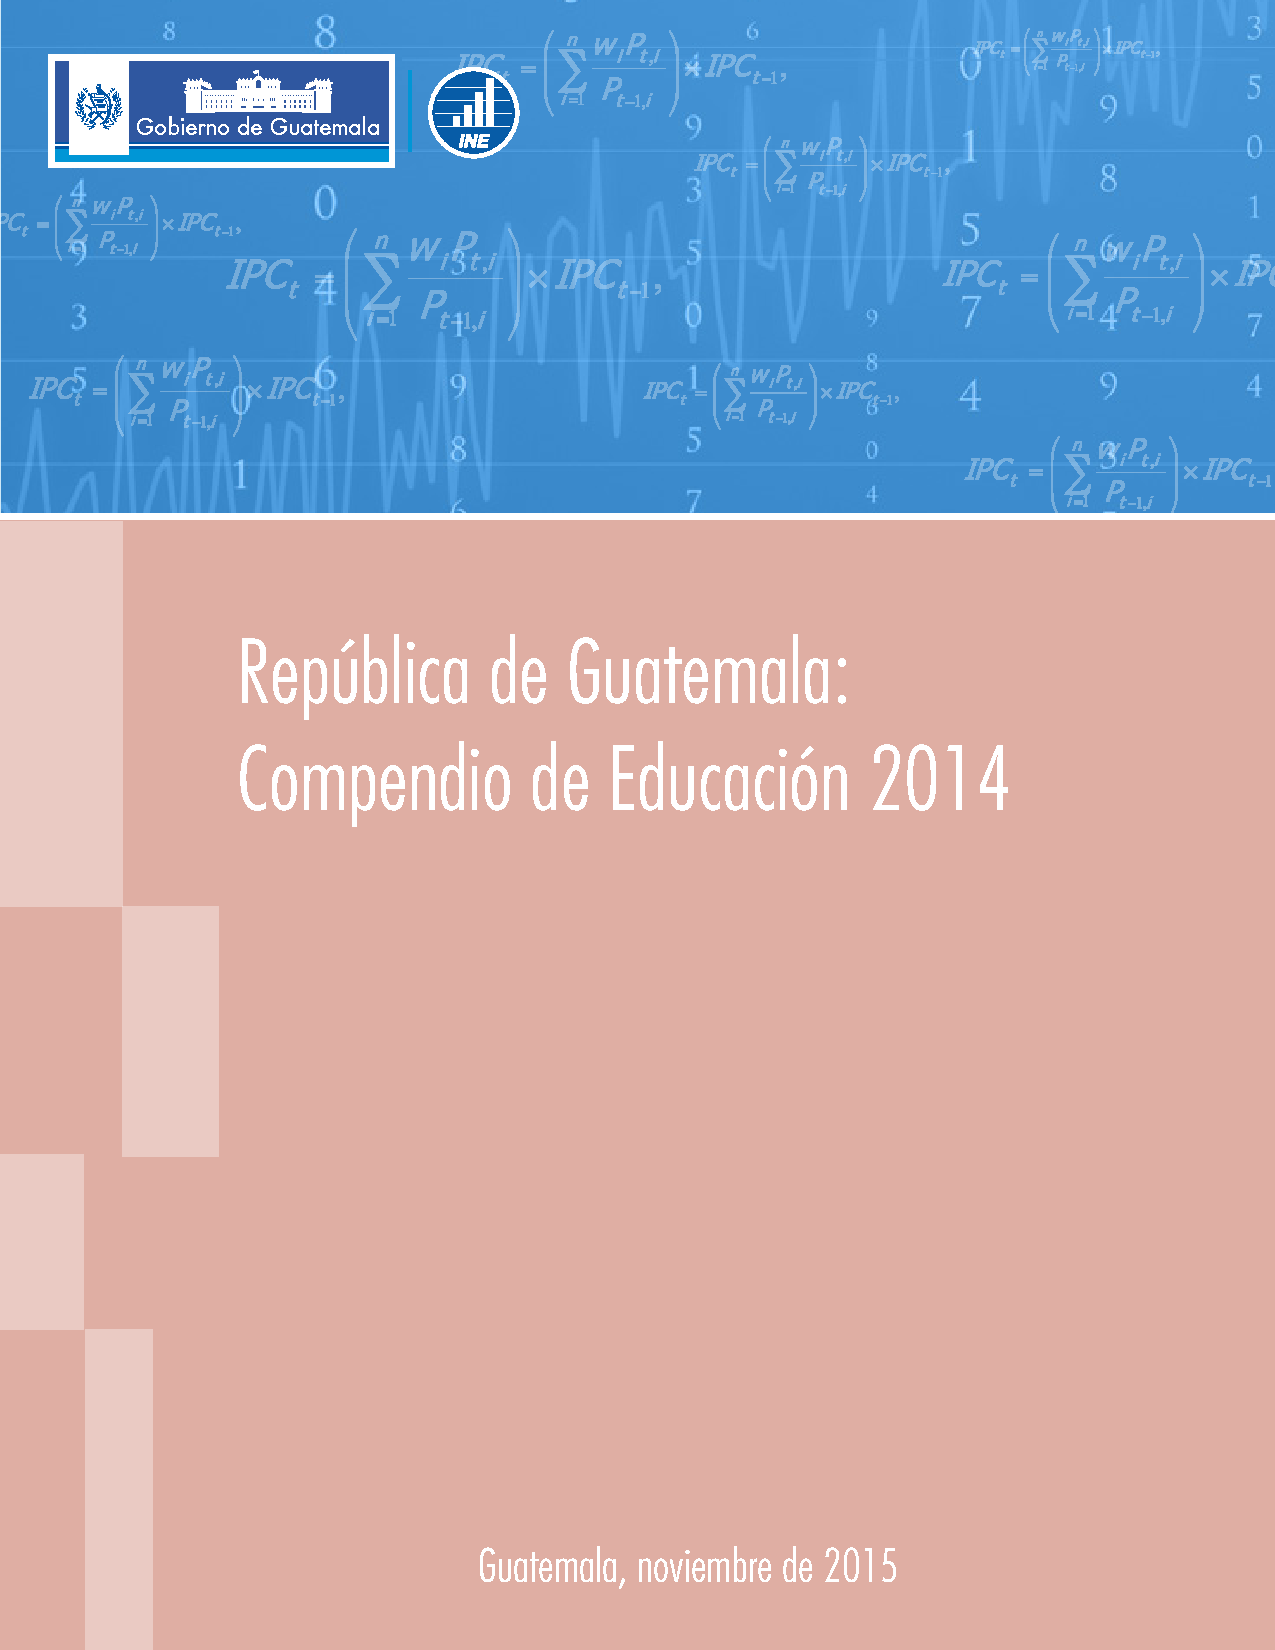
\includepdf{caratula.pdf}
	%
\clearpage

$\ $
\vspace{14.5cm}

\noindent\begin{tabular}{p{0.9cm}p{6.8cm}}
& 2015.$\,$ Guatemala, Centro América \\
&\Bold Instituto Nacional de Estadística\\[-0.4cm]
&\color{blue!50!black}\url{www.ine.gob.gt}\\[0.9cm]
\end{tabular}\\
\noindent\begin{tabular}{p{0.9cm}p{6.8cm}}
& Está permitida la reproducción parcial o total de los contenidos de este documento con la mención de la fuente. \\[0.5cm]
 
& Este documento fue elaborado empleando  {\Sans R}, Inkscape y {\Logos \XeLaTeX}.\\
\end{tabular} 
\pagestyle{empty}

\clearpage


	%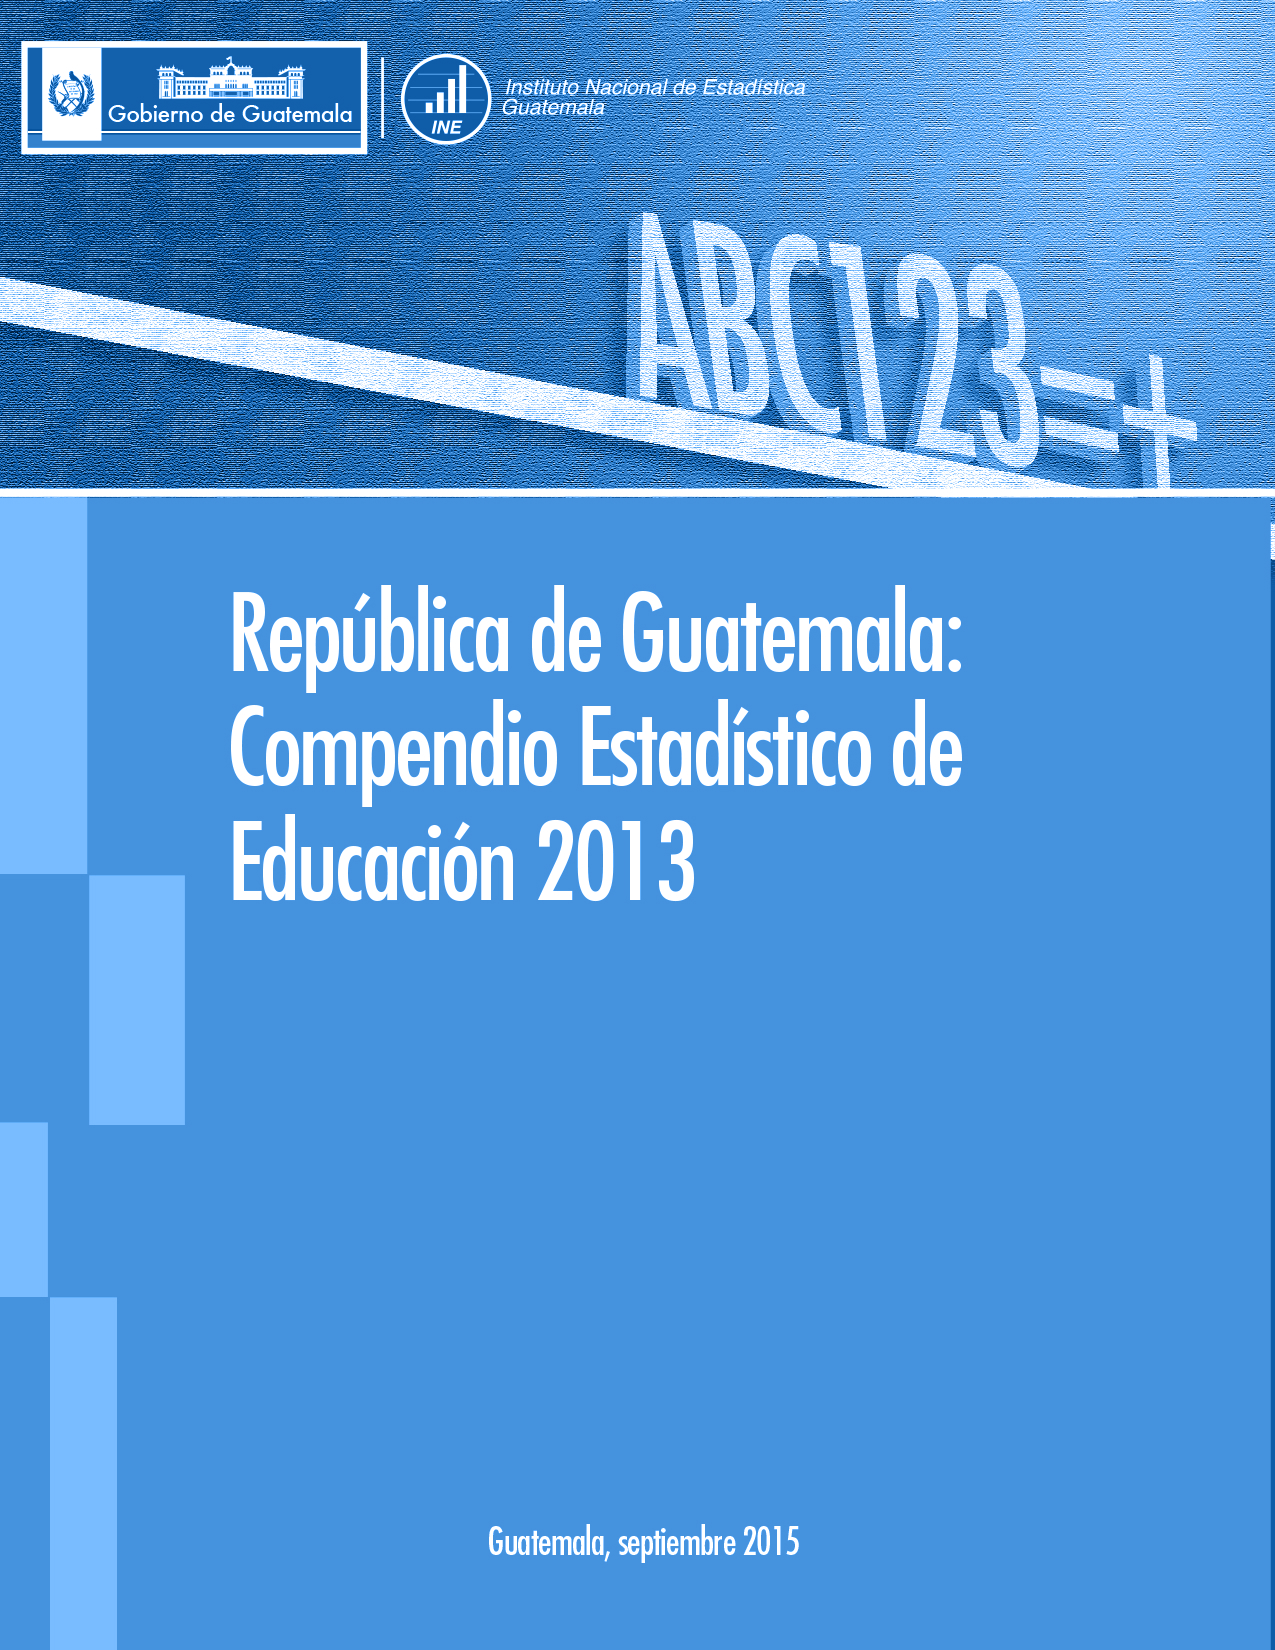
\includepdf{educativa_interior.pdf}
	
	\clearpage
	\newpage $\ $
	\newpage $\ $
$\ $
\vspace{7cm}

\begin{center}
\Bold \LARGE COMPENDIO DE ESTADÍSTICAS DE EDUCACIÓN 2014 \\
\end{center}
\cleardoublepage
$\ $
\vspace{0.0cm}

\begin{center}
	{\Bold \LARGE AUTORIDADES}\\[1cm]
	
	
	{\Bold \large \color{color1!89!black} JUNTA  DIRECTIVA} \\[0.4cm]
	
	{ \Bold Ministerio de Economía}  		\\ 
	Titular: Jorge Méndez Herbruger   \\ 
	Suplente: Jacobo Rey Sigfrido Lee Leiva  \\ [0.4cm] 
	
	{\Bold Ministerio de Finanzas} \\ 
	Titular: Dorval José Carías Samayoa \\ 
	Suplente: Edwin Oswaldo Martínez Cameros\\[0.4cm] 
	
	{\Bold Ministerio de Agricultura, Ganadería y Alimentación} \\ 
	Titular: José Sebastian Marcucci Ruíz   \\ 
	Suplente: Henry Giovanni Vásquez Kilkan \\ [0.4cm] 
	
	{\Bold Ministerio de Energía y Minas}\\ 
	Titular: Juan Pablo Ligorría Arroyo \\ 
	Suplente: Jorge David Calvo Drago\\ [0.4cm]
	{\Bold Secretaría de Planificación y Programación de la Presidencia}   \\
	Titular: Ekaterina Arbolievna Parrilla Artuguina   \\ 
	Suplente: Dora Marina Coc Yup\\ [0.4cm] 
	{\Bold Banco de Guatemala} \\ 
	Titular: Julio Roberto Suárez Guerra \\ 
	Suplente: Sergio Francisco Recinos Rivera\\ [0.4cm] 
	{\Bold Universidad de San Carlos de Guatemala de Guatemala} \\ 
	Titular: Murphy Olimpo Paiz Recinos   \\
	Suplente: Oscar René Paniagua Carrera  \\ [0.4cm]
	{\Bold Universidades Privadas} \\
	Titular: Miguel Ángel Franco de León \\			 Suplente: Ariel Rivera Irías\\ [0.4cm] 
	{\Bold Comité Coordinador de \ Asociaciones  Agrícolas, Comerciales,Industriales y Financieras} \\ 
	Titular: Juan Raúl Aguilar Kaehler \\
	Suplente:  Oscar Augusto Sequeira García  \\ [0.4cm]
	
	{\Bold \large \color{color1!89!black} GERENCIA}\\[0.2cm]
	Gerente:  Rubén Darío Narciso Cruz		\\
	Subgerente Técnico:  Jaime Roberto Mejía Salguero\\
	Subgerente Administrativo Financiero:  Orlando Roberto Monzón Girón\\ 
\end{center}
\cleardoublepage
$\ $
\vspace{-0.3cm}

		\begin{center}
			{\Bold \LARGE Oficina Coordinadora Sectorial de Estadísticas de Educación}\\[.3cm]
			{\Bold \LARGE OCSE - Educación}\\[1cm]
		\end{center}

\begin{multicols}{2}

\begin{center}

	

	\textbf{Instituto Nacional de Estadística}\\
	Coordinador: Gerson Palacios Pantaleón\\ [0.4cm]
	
\textbf{	Secretaría Presidencial de la Mujer – SEPREM}\\
	Titular: Crisalda Lorena Rivera Diaz \\
	Suplente: Mayra López\\ [0.4cm]
	
\textbf{	Secretaría de Planificación y Programación de la Presidencia – SEGEPLAN}\\
	Titular: Edna Abigail Alvarez Och \\
	Suplente: Alma Lucrecia Corzantes\\ [0.4cm]
	
\textbf{	Secretaria Nacional de ciencia y Tecnología  - CONCYT}\\
	Titular: Elías Avilés\\
	Suplente: Ingrid Lorena Menéndez Espinoza \\ [0.4cm]
	
\textbf{	Ministerio de Educación de Guatemala – MINEDUC}\\
	Titular: Mirna Ponciano \\
	Titular: Luisa Muller \\
	Suplente: Mario Contreras \\
	Suplente: Adolfo Santos \\
	Suplente: Mario Quim \\ [0.4cm]
	
\textbf{	Comité Nacional de Alfabetización – CONALFA}\\
	Titular: Edgar Estuardo Ramos Florián\\
	Suplente: Paola Sazo\\ [0.4cm]
	
	\textbf{Instituto Técnico de Capacitación y Productividad – INTECAP}\\
	Titular: Ronald Ochoa\\
	Suplente. Hilda María Robles Flores de Franco\\ [0.4cm]
	
\textbf{	Fondo para la Infancia de las Naciones Unidas – UNICEF}\\
	Titular: Julián Duarte\\
	Suplente: Ileana Cofiño\\ [0.4cm]
	
	\textbf{Programa Nacional de la Competitividad – PRONACOM}\\
	Titular: Maria Isabel Cifuentes\\
	Suplente: Aimeé Rivas de Palma\\ [0.4cm]
	
\textbf{	Consejo de la Enseñanza Privada Superior – CEPS}\\*
	Titular: Sandra Chávez Gálvez\\
	Suplente: Claudia Alejandra Rivera Rivera\\ [0.4cm]
	
\textbf{	Procuraduría de los Derechos Humanos – PDH}\\
	Titular: Julio César Hernández Rodríguez\\
	Suplente: Ariana María Villagrán\\ [0.4cm]
	
\textbf{	Ministerio de Desarrollo Social – MIDES}\\
	Titular: Jorge Luis Diaz Castillo\\
	Suplente: Evelyn López\\ [0.4cm]
	
\textbf{	Gran Campaña por la Educación}\\
	Titular: Ana María Hernández\\ [0.4cm]
	
\textbf{	Organización de las Naciones Unidas para la Educación, la Ciencia y la Cultura - UNESCO }\\
	Titular: Lucía Verdugo\\ [0.4cm]
	
\textbf{	Escuela Nacional Central de Agricultura -ENCA}\\
	Titular: Julio Orantes\\ [0.4cm]
	
\textbf{	Ministerio de la Defensa Nacional – MDF}\\
	Titular: Alfonso Estrada \\ [0.4cm]
	
	\textbf{Ministerio de Finanzas Públicas}\\
	Titular: Rafael Paz\\ [0.4cm]
	
	\textbf{Instituto Centroamericano de Estudios fiscales – ICEFI}\\
	Titular: Alejandra Contreras\\
	Suplente: José Monzón\\ [0.4cm]
	
	\textbf{Universidad del Valle de Guatemala }\\
	Titular: Jorge Andrés Gálvez Sobral Aguilar \\
	Suplente: Jennifer Johnson\\ [0.4cm]
	
	\textbf{Universidad Panamericana}\\
	Titular: Vicky Beatriz Sicajol Calderon\\
	Suplente: Omar Liquez\\ [0.4cm]
	
	\textbf{Universidad Mesoamericana}\\
	Titular: Blanca Nely Galindo\\
	Suplente: Jorge Mario Garoz\\ [0.4cm]
	
	\textbf{Universidad de San Carlos de Guatemala – USAC}\\
	Titular: Aldo Santa Cruz\\ [0.4cm]
	
\textbf{	Universidad Rafael Landívar}\\
	Titular: Pablo Alberto Franky Mendez \\
	Suplente: Nora Lily Muñoz Turcios de García\\ [0.4cm]
	
	\textbf{Universidad del Istmo}\\
	Titular: Mirna de González\\
	Suplente: María Ester Ortega\\ [0.4cm]
	
	\textbf{Universidad InterNaciones}\\
	Titular: Xeyla Rodas\\ [0.4cm]
	
	\textbf{Universidad Galileo}\\
	Titular: Carlos Alberto Oliva Mayorga\\
	Suplente: Julio Israel Santeliz Castañeda\\ [0.4cm]
	
	\textbf{Universidad Mariano Gálvez de Guatemala}\\
	Titular: Ruby Santizo\\ [0.4cm]
	
	\textbf{Universidad San Pablo de Guatemala}\\
	Celeste Aida Oliva Espada\\ [0.4cm]
	
	\textbf{Universidad Rural de Guatemala}\\
	Pamela Galindo\\ [0.4cm]
	
	\textbf{Universidad Francisco Marroquín}\\
	Jessica Paduán\\
	Krista González\\ [0.4cm]
	
	\textbf{Universidad de Occidente}\\
	Beatriz Fernández Lozano\\ [0.4cm]
	
	\textbf{Universidad Da Vinci}\\
	Mónica Álvarez Rivera\\[0.8cm]
	
	
\end{center}

\end{multicols}
\setcounter{page}{0}\cleardoublepage
\clearpage

$\ $
\vspace{1cm}

\begin{center}
	{\Bold \LARGE EQUIPO RESPONSABLE}\\[2cm]
	
	{\Bold \large \color{color1!89!black} REVISIÓN GENERAL}\\[0.2cm]
	Rubén Darío Narciso Cruz\\[0.8cm]
	
	
	{\Bold \large \color{color1!89!black} EQUIPO TÉCNICO}\\[0.2cm]
	Gerson Palacios Pantaleón\\
	Hugo García\\
	Fabiola Ramírez
	
{\Bold \large \color{color1!89!black} DIAGRAMACIÓN Y DISEÑO}\\[0.2cm]
Ligia Morales\\
Fabiola Beatriz Ramírez Pinto\\
Hugo Allan García Monterrosa\\
José Carlos Bonilla Aldana\\[8cm]

\hrule
	Este documento fue elaborado con el apoyo del Fondo para la Infancia de las Naciones Unidas – UNICEF-.\\[0.8cm]


\end{center}\setcounter{page}{0}\cleardoublepage


%\swapgeometry

$\ $\\[1cm]

\tableofcontents

\cleardoublepage
	\pagestyle{estandar}
	\setcounter{page}{1}
	\setlength{\arrayrulewidth}{1.0pt}





\cleardoublepage


$\ $\\[2cm]
\noindent {\Bold \huge Presentación}

 La educación es un elemento clave para el desarrollo de las personas y los estados. Tal es así, que la Declaración Universal de los Derechos Humanos de 1948 establece: “Toda persona tiene derecho a la educación. La educación debe ser gratuita, al menos en lo concerniente a la instrucción elemental y fundamental. La instrucción elemental será obligatoria”.
 
 Por esa razón, y atendiendo al mandato institucional expresados en el Decreto Ley 3-85,la Junta Directiva del Instituto Nacional de Estadística INE, a través de la resolución JD-09/10/2014 del acta número JD-09/2014 creó la Unidad de Estadísticas de Educación así como la Oficina Coordinadora Sectorial de Estadísticas (OCSE) de Educación, órganos que tienen como principal función recabar información estadística educativa que permita diseñar, evaluar y monitorear políticas públicas en esta importante materia.
 
 Como resultado del trabajo de la Unidad y la Oficina Coordinadora Sectorial de Estadísticas de Educación, se presenta el \textbf{Compendio estadístico de educación 2014}, el cual se encuentra dividido en cinco partes:
 
\begin{itemize}
	\item Estadísticas de los niveles educativos a cargo del Ministerio de  Educación
	\item Estadísticas de educación superior
	\item Educación y empleo
	\item Educación y fecundidad
	\item Gasto en educación
\end{itemize}


Los datos contenidos en el compendio fueron obtenidos de la Encuesta Nacional de Condiciones de Vida (ENCOVI), Encuesta Nacional de Empleo e Ingresos (ENEI), datos de las Estadísticas Vitales, información sobre estadística inicial del Ministerio de Educación (MINEDUC), datos del Ministerio de Finanzas Públicas (MINFIN) e información proporcionada por las universidades del país, todos ellos validos y discutidos dentro del seno de la mesa técnica de la OCSE de educación.

El INE agradece enormemente el apoyo brindado por las distintas instituciones que proporcionaron información para el Compendio estadístico de educación 2014 el cual sin duda será un insumo valioso para las distintas organizaciones que velan por el bienestar de la población guatemalteca.

\restoregeometry

	\thispagestyle{estandar}


%\INEpartecarta[Estadísticas de los niveles educativos a cargo del\\ Ministerio de Educación]{Estadísticas de los niveles educativos a cargo del Ministerio de Educación}{}
%
%\INEchaptercarta{Alumnos en preprimaria}{}



\cajita{Inscritos }{El número de  inscritos en preprimaria se obtiene a partir del total de los alumnos sin importar la edad, registrados al treinta de marzo de cada ciclo escolar\llamada. \textollamada{También se le llama estadística inicial} 
	
	En el 2009 se inscribieron 584,833 alumnos y en el 2013 se inscribieron 543,226 alumnos, lo cual representa un incremento del 13.7\%.}{Número de inscritos en el ciclo de educación preprimaria}{República de Guatemala, serie histórica, en datos absolutos}{\ \\[0mm]\begin{tikzpicture}[x=1pt,y=1pt]  % Created by tikzDevice version 0.7.0 on 2015-08-28 13:12:28
% !TEX encoding = UTF-8 Unicode
\definecolor[named]{fillColor}{rgb}{1.00,1.00,1.00}
\path[use as bounding box,fill=fillColor,fill opacity=0.00] (0,0) rectangle (289.08,198.74);
\begin{scope}
\path[clip] (  0.00,  0.00) rectangle (289.08,198.74);
\definecolor[named]{drawColor}{rgb}{1.00,1.00,1.00}

\path[draw=drawColor,line width= 0.6pt,line join=round,line cap=round] (  0.00,  0.00) rectangle (289.08,198.74);
\end{scope}
\begin{scope}
\path[clip] (  0.00,  0.00) rectangle (289.08,198.74);

\path[] ( 14.70, 17.78) rectangle (280.54,191.48);

\path[] ( 14.70, 52.66) --
	(280.54, 52.66);

\path[] ( 14.70,106.67) --
	(280.54,106.67);

\path[] ( 14.70,160.68) --
	(280.54,160.68);

\path[] ( 14.70, 25.65) --
	(280.54, 25.65);

\path[] ( 14.70, 79.66) --
	(280.54, 79.66);

\path[] ( 14.70,133.67) --
	(280.54,133.67);

\path[] ( 14.70,187.68) --
	(280.54,187.68);

\path[] ( 45.37, 17.78) --
	( 45.37,191.48);

\path[] ( 96.50, 17.78) --
	( 96.50,191.48);

\path[] (147.62, 17.78) --
	(147.62,191.48);

\path[] (198.74, 17.78) --
	(198.74,191.48);

\path[] (249.87, 17.78) --
	(249.87,191.48);
\definecolor[named]{drawColor}{rgb}{0.00,0.00,1.00}

\path[draw=drawColor,line width= 1.7pt,line join=round] ( 45.37,183.59) --
	( 96.50,181.68) --
	(147.62,179.10) --
	(198.74,171.33) --
	(249.87,172.35);
\definecolor[named]{drawColor}{rgb}{0.00,0.00,0.00}

\node[text=drawColor,anchor=base,inner sep=0pt, outer sep=0pt, scale=  1.01] at ( 45.37,187.54) {584,833};

\node[text=drawColor,anchor=base west,inner sep=0pt, outer sep=0pt, scale=  1.01] at ( 96.50,185.64) {577,766};

\node[text=drawColor,anchor=base west,inner sep=0pt, outer sep=0pt, scale=  1.01] at (147.62,183.06) {568,225};

\node[text=drawColor,anchor=base,inner sep=0pt, outer sep=0pt, scale=  1.01] at (198.74,159.46) {539,462};

\node[text=drawColor,anchor=base,inner sep=0pt, outer sep=0pt, scale=  1.01] at (249.87,176.31) {543,226};
\definecolor[named]{fillColor}{rgb}{0.00,0.00,0.00}

\path[draw=drawColor,line width= 0.1pt,line join=round,fill=fillColor] ( 14.70, 25.67) -- (280.54, 25.67);
\end{scope}
\begin{scope}
\path[clip] (  0.00,  0.00) rectangle (289.08,198.74);

\path[] ( 14.70, 17.78) --
	( 14.70,191.48);
\end{scope}
\begin{scope}
\path[clip] (  0.00,  0.00) rectangle (289.08,198.74);
\definecolor[named]{drawColor}{rgb}{1.00,1.00,1.00}

\node[text=drawColor,text opacity=0.00,anchor=base east,inner sep=0pt, outer sep=0pt, scale=  1.00] at (  7.58, 21.75) {0e+00};

\node[text=drawColor,text opacity=0.00,anchor=base east,inner sep=0pt, outer sep=0pt, scale=  1.00] at (  7.58, 75.76) {2e+05};

\node[text=drawColor,text opacity=0.00,anchor=base east,inner sep=0pt, outer sep=0pt, scale=  1.00] at (  7.58,129.77) {4e+05};

\node[text=drawColor,text opacity=0.00,anchor=base east,inner sep=0pt, outer sep=0pt, scale=  1.00] at (  7.58,183.77) {6e+05};
\end{scope}
\begin{scope}
\path[clip] (  0.00,  0.00) rectangle (289.08,198.74);

\path[] ( 10.43, 25.65) --
	( 14.70, 25.65);

\path[] ( 10.43, 79.66) --
	( 14.70, 79.66);

\path[] ( 10.43,133.67) --
	( 14.70,133.67);

\path[] ( 10.43,187.68) --
	( 14.70,187.68);
\end{scope}
\begin{scope}
\path[clip] (  0.00,  0.00) rectangle (289.08,198.74);

\path[] ( 14.70, 17.78) --
	(280.54, 17.78);
\end{scope}
\begin{scope}
\path[clip] (  0.00,  0.00) rectangle (289.08,198.74);

\path[] ( 45.37, 13.51) --
	( 45.37, 17.78);

\path[] ( 96.50, 13.51) --
	( 96.50, 17.78);

\path[] (147.62, 13.51) --
	(147.62, 17.78);

\path[] (198.74, 13.51) --
	(198.74, 17.78);

\path[] (249.87, 13.51) --
	(249.87, 17.78);
\end{scope}
\begin{scope}
\path[clip] (  0.00,  0.00) rectangle (289.08,198.74);
\definecolor[named]{drawColor}{rgb}{0.00,0.00,0.00}

\node[text=drawColor,anchor=base,inner sep=0pt, outer sep=0pt, scale=  1.00] at ( 45.37,  2.85) {2009};

\node[text=drawColor,anchor=base,inner sep=0pt, outer sep=0pt, scale=  1.00] at ( 96.50,  2.85) {2010};

\node[text=drawColor,anchor=base,inner sep=0pt, outer sep=0pt, scale=  1.00] at (147.62,  2.85) {2011};

\node[text=drawColor,anchor=base,inner sep=0pt, outer sep=0pt, scale=  1.00] at (198.74,  2.85) {2012};

\node[text=drawColor,anchor=base,inner sep=0pt, outer sep=0pt, scale=  1.00] at (249.87,  2.85) {2014};
\end{scope}
  \end{tikzpicture}}{Instituto Nacional de Estadística, con datos del Ministerio de Educación}

\cajita{Inscritos por sexo}{La distribución de alumnos inscritos en educación preprimaria según su sexo, muestra que el 50.5\% fueron hombres, mayor en 1 punto porcentual respecto a las mujeres.}{Distribución de inscritos en el ciclo de\\ educación preprimaria, por sexo}{República de Guatemala, año 2013, en porcentaje}{\ \\[0mm]\begin{tikzpicture}[x=1pt,y=1pt]  % Created by tikzDevice version 0.10.1 on 2016-02-29 12:41:01
% !TEX encoding = UTF-8 Unicode
\definecolor{fillColor}{RGB}{255,255,255}
\path[use as bounding box,fill=fillColor,fill opacity=0.00] (0,0) rectangle (289.08,198.74);
\begin{scope}
\path[clip] ( 30.54,  0.00) rectangle (258.54,198.74);

\path[] ( 30.54,  0.00) rectangle (258.54,198.74);
\end{scope}
\begin{scope}
\path[clip] (  0.00,  0.00) rectangle (289.08,198.74);

\path[] (  7.11,  4.95) rectangle (200.91,198.74);

\path[] (104.01,101.85) --
	(191.21,100.67);

\path[] (104.01,101.85) --
	( 16.81,103.03);

\path[] (104.01,101.85) --
	(105.19,189.04);

\path[] (104.01,101.85) --
	(191.21,100.67);

\path[] (104.01,101.85) --
	(102.83, 14.65);

\path[] (104.01,101.85) --
	( 16.81,103.03);

\path[] (104.01,101.85) --
	(104.01,101.85) --
	(104.01,101.85) --
	(104.01,101.85) --
	(104.01,101.85) --
	(104.01,101.85) --
	(104.01,101.85) --
	(104.01,101.85) --
	(104.01,101.85) --
	(104.01,101.85) --
	(104.01,101.85) --
	(104.01,101.85) --
	(104.01,101.85) --
	(104.01,101.85) --
	(104.01,101.85) --
	(104.01,101.85) --
	(104.01,101.85) --
	(104.01,101.85) --
	(104.01,101.85) --
	(104.01,101.85) --
	(104.01,101.85) --
	(104.01,101.85) --
	(104.01,101.85) --
	(104.01,101.85) --
	(104.01,101.85) --
	(104.01,101.85) --
	(104.01,101.85) --
	(104.01,101.85) --
	(104.01,101.85) --
	(104.01,101.85) --
	(104.01,101.85) --
	(104.01,101.85) --
	(104.01,101.85) --
	(104.01,101.85) --
	(104.01,101.85) --
	(104.01,101.85) --
	(104.01,101.85) --
	(104.01,101.85) --
	(104.01,101.85) --
	(104.01,101.85) --
	(104.01,101.85) --
	(104.01,101.85) --
	(104.01,101.85) --
	(104.01,101.85) --
	(104.01,101.85) --
	(104.01,101.85) --
	(104.01,101.85) --
	(104.01,101.85) --
	(104.01,101.85) --
	(104.01,101.85) --
	(104.01,101.85) --
	(104.01,101.85) --
	(104.01,101.85) --
	(104.01,101.85) --
	(104.01,101.85) --
	(104.01,101.85) --
	(104.01,101.85) --
	(104.01,101.85) --
	(104.01,101.85) --
	(104.01,101.85) --
	(104.01,101.85) --
	(104.01,101.85) --
	(104.01,101.85) --
	(104.01,101.85) --
	(104.01,101.85) --
	(104.01,101.85) --
	(104.01,101.85) --
	(104.01,101.85) --
	(104.01,101.85) --
	(104.01,101.85) --
	(104.01,101.85) --
	(104.01,101.85) --
	(104.01,101.85) --
	(104.01,101.85) --
	(104.01,101.85) --
	(104.01,101.85) --
	(104.01,101.85) --
	(104.01,101.85) --
	(104.01,101.85) --
	(104.01,101.85) --
	(104.01,101.85) --
	(104.01,101.85) --
	(104.01,101.85) --
	(104.01,101.85) --
	(104.01,101.85) --
	(104.01,101.85) --
	(104.01,101.85) --
	(104.01,101.85) --
	(104.01,101.85) --
	(104.01,101.85) --
	(104.01,101.85) --
	(104.01,101.85) --
	(104.01,101.85) --
	(104.01,101.85) --
	(104.01,101.85) --
	(104.01,101.85) --
	(104.01,101.85) --
	(104.01,101.85) --
	(104.01,101.85) --
	(104.01,101.85);

\path[] (104.01,121.23) --
	(105.24,121.19) --
	(106.46,121.07) --
	(107.68,120.88) --
	(108.88,120.60) --
	(110.06,120.26) --
	(111.21,119.84) --
	(112.34,119.34) --
	(113.43,118.78) --
	(114.49,118.15) --
	(115.50,117.45) --
	(116.47,116.69) --
	(117.38,115.87) --
	(118.25,115.00) --
	(119.05,114.07) --
	(119.80,113.09) --
	(120.48,112.06) --
	(121.09,111.00) --
	(121.64,109.90) --
	(122.11,108.76) --
	(122.51,107.60) --
	(122.84,106.42) --
	(123.09,105.21) --
	(123.27,103.99) --
	(123.37,102.77) --
	(123.39,101.54) --
	(123.33,100.31) --
	(123.19, 99.09) --
	(122.98, 97.88) --
	(122.69, 96.68) --
	(122.32, 95.51) --
	(121.88, 94.36) --
	(121.37, 93.24) --
	(120.79, 92.16) --
	(120.14, 91.11) --
	(119.43, 90.11) --
	(118.66, 89.16) --
	(117.82, 88.25) --
	(116.93, 87.40) --
	(115.99, 86.61) --
	(115.00, 85.88) --
	(113.96, 85.22) --
	(112.89, 84.62) --
	(111.78, 84.09) --
	(110.64, 83.64) --
	(109.47, 83.25) --
	(108.28, 82.94) --
	(107.07, 82.71) --
	(105.85, 82.55) --
	(104.62, 82.48) --
	(103.39, 82.48) --
	(102.17, 82.55) --
	(100.95, 82.71) --
	( 99.74, 82.94) --
	( 98.55, 83.25) --
	( 97.38, 83.64) --
	( 96.24, 84.09) --
	( 95.13, 84.62) --
	( 94.05, 85.22) --
	( 93.02, 85.88) --
	( 92.03, 86.61) --
	( 91.09, 87.40) --
	( 90.20, 88.25) --
	( 89.36, 89.16) --
	( 88.59, 90.11) --
	( 87.87, 91.11) --
	( 87.23, 92.16) --
	( 86.65, 93.24) --
	( 86.13, 94.36) --
	( 85.70, 95.51) --
	( 85.33, 96.68) --
	( 85.04, 97.88) --
	( 84.83, 99.09) --
	( 84.69,100.31) --
	( 84.63,101.54) --
	( 84.65,102.77) --
	( 84.75,103.99) --
	( 84.92,105.21) --
	( 85.18,106.42) --
	( 85.50,107.60) --
	( 85.91,108.76) --
	( 86.38,109.90) --
	( 86.93,111.00) --
	( 87.54,112.06) --
	( 88.22,113.09) --
	( 88.97,114.07) --
	( 89.77,115.00) --
	( 90.64,115.87) --
	( 91.55,116.69) --
	( 92.52,117.45) --
	( 93.53,118.15) --
	( 94.59,118.78) --
	( 95.68,119.34) --
	( 96.81,119.84) --
	( 97.96,120.26) --
	( 99.14,120.60) --
	(100.34,120.88) --
	(101.56,121.07) --
	(102.78,121.19) --
	(104.01,121.23);

\path[] (104.01,140.60) --
	(106.47,140.53) --
	(108.92,140.29) --
	(111.34,139.90) --
	(113.74,139.36) --
	(116.10,138.67) --
	(118.41,137.83) --
	(120.67,136.84) --
	(122.85,135.72) --
	(124.96,134.45) --
	(126.99,133.06) --
	(128.92,131.54) --
	(130.76,129.90) --
	(132.48,128.14) --
	(134.09,126.29) --
	(135.58,124.33) --
	(136.94,122.28) --
	(138.17,120.15) --
	(139.27,117.95) --
	(140.22,115.68) --
	(141.02,113.35) --
	(141.68,110.98) --
	(142.18,108.58) --
	(142.53,106.14) --
	(142.72,103.69) --
	(142.76,101.23) --
	(142.65, 98.77) --
	(142.37, 96.33) --
	(141.95, 93.91) --
	(141.37, 91.52) --
	(140.64, 89.17) --
	(139.76, 86.87) --
	(138.74, 84.63) --
	(137.58, 82.47) --
	(136.28, 80.38) --
	(134.85, 78.37) --
	(133.30, 76.46) --
	(131.63, 74.66) --
	(129.85, 72.96) --
	(127.97, 71.38) --
	(125.99, 69.92) --
	(123.92, 68.59) --
	(121.77, 67.40) --
	(119.55, 66.34) --
	(117.27, 65.43) --
	(114.93, 64.66) --
	(112.55, 64.04) --
	(110.13, 63.57) --
	(107.69, 63.26) --
	(105.24, 63.11) --
	(102.78, 63.11) --
	(100.33, 63.26) --
	( 97.89, 63.57) --
	( 95.47, 64.04) --
	( 93.09, 64.66) --
	( 90.75, 65.43) --
	( 88.47, 66.34) --
	( 86.25, 67.40) --
	( 84.10, 68.59) --
	( 82.03, 69.92) --
	( 80.05, 71.38) --
	( 78.17, 72.96) --
	( 76.39, 74.66) --
	( 74.72, 76.46) --
	( 73.17, 78.37) --
	( 71.74, 80.38) --
	( 70.44, 82.47) --
	( 69.28, 84.63) --
	( 68.26, 86.87) --
	( 67.38, 89.17) --
	( 66.65, 91.52) --
	( 66.07, 93.91) --
	( 65.65, 96.33) --
	( 65.37, 98.77) --
	( 65.26,101.23) --
	( 65.29,103.69) --
	( 65.49,106.14) --
	( 65.84,108.58) --
	( 66.34,110.98) --
	( 67.00,113.35) --
	( 67.80,115.68) --
	( 68.75,117.95) --
	( 69.85,120.15) --
	( 71.08,122.28) --
	( 72.44,124.33) --
	( 73.93,126.29) --
	( 75.54,128.14) --
	( 77.26,129.90) --
	( 79.10,131.54) --
	( 81.03,133.06) --
	( 83.06,134.45) --
	( 85.17,135.72) --
	( 87.35,136.84) --
	( 89.60,137.83) --
	( 91.92,138.67) --
	( 94.28,139.36) --
	( 96.67,139.90) --
	( 99.10,140.29) --
	(101.55,140.53) --
	(104.01,140.60);

\path[] (104.01,159.98) --
	(107.70,159.87) --
	(111.37,159.52) --
	(115.01,158.93) --
	(118.61,158.12) --
	(122.15,157.08) --
	(125.62,155.82) --
	(129.00,154.34) --
	(132.28,152.65) --
	(135.44,150.75) --
	(138.48,148.66) --
	(141.38,146.38) --
	(144.13,143.92) --
	(146.72,141.29) --
	(149.13,138.51) --
	(151.37,135.57) --
	(153.41,132.50) --
	(155.26,129.30) --
	(156.89,126.00) --
	(158.32,122.59) --
	(159.53,119.11) --
	(160.51,115.55) --
	(161.26,111.94) --
	(161.79,108.29) --
	(162.08,104.61) --
	(162.14,100.92) --
	(161.96, 97.24) --
	(161.56, 93.57) --
	(160.91, 89.94) --
	(160.05, 86.35) --
	(158.95, 82.83) --
	(157.63, 79.39) --
	(156.10, 76.03) --
	(154.36, 72.78) --
	(152.41, 69.64) --
	(150.27, 66.64) --
	(147.95, 63.77) --
	(145.44, 61.06) --
	(142.77, 58.52) --
	(139.95, 56.15) --
	(136.98, 53.96) --
	(133.87, 51.97) --
	(130.65, 50.17) --
	(127.32, 48.59) --
	(123.89, 47.21) --
	(120.39, 46.06) --
	(116.82, 45.14) --
	(113.20, 44.44) --
	(109.54, 43.97) --
	(105.85, 43.74) --
	(102.16, 43.74) --
	( 98.48, 43.97) --
	( 94.82, 44.44) --
	( 91.20, 45.14) --
	( 87.63, 46.06) --
	( 84.13, 47.21) --
	( 80.70, 48.59) --
	( 77.37, 50.17) --
	( 74.15, 51.97) --
	( 71.04, 53.96) --
	( 68.07, 56.15) --
	( 65.25, 58.52) --
	( 62.58, 61.06) --
	( 60.07, 63.77) --
	( 57.75, 66.64) --
	( 55.61, 69.64) --
	( 53.66, 72.78) --
	( 51.92, 76.03) --
	( 50.39, 79.39) --
	( 49.07, 82.83) --
	( 47.97, 86.35) --
	( 47.10, 89.94) --
	( 46.46, 93.57) --
	( 46.05, 97.24) --
	( 45.88,100.92) --
	( 45.94,104.61) --
	( 46.23,108.29) --
	( 46.75,111.94) --
	( 47.51,115.55) --
	( 48.49,119.11) --
	( 49.70,122.59) --
	( 51.13,126.00) --
	( 52.76,129.30) --
	( 54.61,132.50) --
	( 56.65,135.57) --
	( 58.89,138.51) --
	( 61.30,141.29) --
	( 63.89,143.92) --
	( 66.64,146.38) --
	( 69.54,148.66) --
	( 72.58,150.75) --
	( 75.74,152.65) --
	( 79.02,154.34) --
	( 82.40,155.82) --
	( 85.87,157.08) --
	( 89.41,158.12) --
	( 93.01,158.93) --
	( 96.65,159.52) --
	(100.32,159.87) --
	(104.01,159.98);

\path[] (104.01,179.36) --
	(108.93,179.21) --
	(113.82,178.74) --
	(118.68,177.96) --
	(123.48,176.88) --
	(128.20,175.49) --
	(132.82,173.81) --
	(137.33,171.84) --
	(141.70,169.58) --
	(145.92,167.06) --
	(149.97,164.27) --
	(153.84,161.23) --
	(157.50,157.95) --
	(160.95,154.44) --
	(164.17,150.72) --
	(167.15,146.81) --
	(169.88,142.72) --
	(172.34,138.46) --
	(174.52,134.05) --
	(176.42,129.51) --
	(178.03,124.86) --
	(179.34,120.12) --
	(180.35,115.31) --
	(181.05,110.44) --
	(181.44,105.53) --
	(181.52,100.62) --
	(181.28, 95.70) --
	(180.74, 90.81) --
	(179.88, 85.97) --
	(178.72, 81.19) --
	(177.26, 76.49) --
	(175.51, 71.90) --
	(173.46, 67.42) --
	(171.14, 63.09) --
	(168.55, 58.91) --
	(165.69, 54.90) --
	(162.59, 51.08) --
	(159.26, 47.47) --
	(155.70, 44.08) --
	(151.93, 40.91) --
	(147.97, 38.00) --
	(143.83, 35.34) --
	(139.53, 32.95) --
	(135.09, 30.83) --
	(130.52, 29.00) --
	(125.85, 27.47) --
	(121.09, 26.23) --
	(116.26, 25.30) --
	(111.38, 24.68) --
	(106.47, 24.37) --
	(101.55, 24.37) --
	( 96.64, 24.68) --
	( 91.76, 25.30) --
	( 86.93, 26.23) --
	( 82.17, 27.47) --
	( 77.50, 29.00) --
	( 72.93, 30.83) --
	( 68.49, 32.95) --
	( 64.19, 35.34) --
	( 60.05, 38.00) --
	( 56.09, 40.91) --
	( 52.32, 44.08) --
	( 48.76, 47.47) --
	( 45.43, 51.08) --
	( 42.32, 54.90) --
	( 39.47, 58.91) --
	( 36.88, 63.09) --
	( 34.55, 67.42) --
	( 32.51, 71.90) --
	( 30.76, 76.49) --
	( 29.30, 81.19) --
	( 28.14, 85.97) --
	( 27.28, 90.81) --
	( 26.74, 95.70) --
	( 26.50,100.62) --
	( 26.58,105.53) --
	( 26.97,110.44) --
	( 27.67,115.31) --
	( 28.68,120.12) --
	( 29.99,124.86) --
	( 31.60,129.51) --
	( 33.50,134.05) --
	( 35.68,138.46) --
	( 38.14,142.72) --
	( 40.87,146.81) --
	( 43.84,150.72) --
	( 47.07,154.44) --
	( 50.52,157.95) --
	( 54.18,161.23) --
	( 58.05,164.27) --
	( 62.10,167.06) --
	( 66.32,169.58) --
	( 70.69,171.84) --
	( 75.20,173.81) --
	( 79.82,175.49) --
	( 84.54,176.88) --
	( 89.34,177.96) --
	( 94.20,178.74) --
	( 99.09,179.21) --
	(104.01,179.36);

\path[] (104.01,189.05) --
	(109.54,188.88) --
	(115.05,188.35) --
	(120.51,187.48) --
	(125.91,186.26) --
	(131.22,184.70) --
	(136.42,182.81) --
	(141.49,180.59) --
	(146.41,178.05) --
	(151.16,175.21) --
	(155.71,172.07) --
	(160.06,168.65) --
	(164.19,164.96) --
	(168.07,161.02) --
	(171.69,156.83) --
	(175.05,152.43) --
	(178.11,147.82) --
	(180.88,143.03) --
	(183.34,138.07) --
	(185.47,132.97) --
	(187.28,127.74) --
	(188.76,122.41) --
	(189.89,116.99) --
	(190.68,111.51) --
	(191.12,106.00) --
	(191.21,100.46) --
	(190.94, 94.94) --
	(190.33, 89.44) --
	(189.37, 83.99) --
	(188.06, 78.61) --
	(186.42, 73.32) --
	(184.44, 68.15) --
	(182.15, 63.12) --
	(179.53, 58.24) --
	(176.62, 53.54) --
	(173.41, 49.03) --
	(169.92, 44.74) --
	(166.16, 40.67) --
	(162.16, 36.85) --
	(157.92, 33.30) --
	(153.46, 30.02) --
	(148.81, 27.02) --
	(143.97, 24.33) --
	(138.97, 21.96) --
	(133.84, 19.90) --
	(128.58, 18.17) --
	(123.22, 16.78) --
	(117.79, 15.74) --
	(112.30, 15.03) --
	(106.78, 14.68) --
	(101.24, 14.68) --
	( 95.72, 15.03) --
	( 90.23, 15.74) --
	( 84.80, 16.78) --
	( 79.44, 18.17) --
	( 74.18, 19.90) --
	( 69.05, 21.96) --
	( 64.05, 24.33) --
	( 59.21, 27.02) --
	( 54.56, 30.02) --
	( 50.10, 33.30) --
	( 45.86, 36.85) --
	( 41.86, 40.67) --
	( 38.10, 44.74) --
	( 34.61, 49.03) --
	( 31.40, 53.54) --
	( 28.49, 58.24) --
	( 25.87, 63.12) --
	( 23.57, 68.15) --
	( 21.60, 73.32) --
	( 19.96, 78.61) --
	( 18.65, 83.99) --
	( 17.69, 89.44) --
	( 17.08, 94.94) --
	( 16.81,100.46) --
	( 16.90,106.00) --
	( 17.34,111.51) --
	( 18.13,116.99) --
	( 19.26,122.41) --
	( 20.74,127.74) --
	( 22.55,132.97) --
	( 24.68,138.07) --
	( 27.14,143.03) --
	( 29.91,147.82) --
	( 32.97,152.43) --
	( 36.32,156.83) --
	( 39.95,161.02) --
	( 43.83,164.96) --
	( 47.95,168.65) --
	( 52.30,172.07) --
	( 56.86,175.21) --
	( 61.61,178.05) --
	( 66.53,180.59) --
	( 71.60,182.81) --
	( 76.80,184.70) --
	( 82.11,186.26) --
	( 87.51,187.48) --
	( 92.97,188.35) --
	( 98.48,188.88) --
	(104.01,189.05);
\definecolor{drawColor}{RGB}{255,255,255}
\definecolor{fillColor}{RGB}{0,0,255}

\path[draw=drawColor,line width= 0.6pt,line join=round,line cap=round,fill=fillColor] (102.96, 63.10) --
	(102.89, 60.33) --
	(102.81, 57.57) --
	(102.74, 54.80) --
	(102.66, 52.03) --
	(102.59, 49.26) --
	(102.51, 46.50) --
	(102.44, 43.73) --
	(102.36, 40.96) --
	(102.29, 38.19) --
	(102.21, 35.43) --
	(102.14, 32.66) --
	(102.06, 29.89) --
	(101.99, 27.13) --
	(101.91, 24.36) --
	(104.55, 24.33) --
	(107.19, 24.39) --
	(109.83, 24.55) --
	(112.46, 24.79) --
	(115.08, 25.12) --
	(117.69, 25.55) --
	(120.28, 26.06) --
	(122.85, 26.65) --
	(125.40, 27.34) --
	(127.93, 28.11) --
	(130.42, 28.97) --
	(132.89, 29.91) --
	(135.33, 30.94) --
	(137.72, 32.04) --
	(140.08, 33.23) --
	(142.40, 34.50) --
	(144.67, 35.85) --
	(146.89, 37.27) --
	(149.07, 38.77) --
	(151.19, 40.34) --
	(153.26, 41.98) --
	(155.27, 43.70) --
	(157.22, 45.48) --
	(159.11, 47.32) --
	(160.94, 49.23) --
	(162.69, 51.20) --
	(164.39, 53.23) --
	(166.01, 55.31) --
	(167.56, 57.45) --
	(169.03, 59.64) --
	(170.43, 61.88) --
	(171.75, 64.17) --
	(173.00, 66.50) --
	(174.16, 68.87) --
	(175.24, 71.28) --
	(176.24, 73.72) --
	(177.16, 76.20) --
	(177.99, 78.71) --
	(178.74, 81.24) --
	(179.40, 83.80) --
	(179.97, 86.38) --
	(180.45, 88.97) --
	(180.84, 91.58) --
	(181.15, 94.21) --
	(181.36, 96.84) --
	(181.49, 99.48) --
	(181.53,102.12) --
	(181.47,104.76) --
	(181.33,107.40) --
	(181.09,110.03) --
	(180.77,112.65) --
	(180.36,115.26) --
	(179.86,117.85) --
	(179.27,120.42) --
	(178.59,122.98) --
	(177.83,125.50) --
	(176.98,128.01) --
	(176.05,130.48) --
	(175.03,132.91) --
	(173.93,135.31) --
	(172.75,137.68) --
	(171.49,140.00) --
	(170.15,142.27) --
	(168.73,144.50) --
	(167.24,146.68) --
	(165.68,148.81) --
	(164.04,150.89) --
	(162.34,152.90) --
	(160.56,154.86) --
	(158.73,156.76) --
	(156.82,158.59) --
	(154.86,160.35) --
	(152.84,162.05) --
	(150.76,163.68) --
	(148.63,165.24) --
	(146.44,166.72) --
	(144.21,168.13) --
	(141.92,169.46) --
	(139.60,170.71) --
	(137.23,171.88) --
	(134.83,172.97) --
	(132.39,173.98) --
	(129.91,174.91) --
	(127.41,175.75) --
	(124.88,176.50) --
	(122.32,177.17) --
	(119.75,177.75) --
	(117.15,178.24) --
	(114.54,178.64) --
	(111.92,178.96) --
	(109.29,179.18) --
	(106.65,179.32) --
	(104.01,179.36) --
	(104.01,176.59) --
	(104.01,173.83) --
	(104.01,171.06) --
	(104.01,168.29) --
	(104.01,165.52) --
	(104.01,162.75) --
	(104.01,159.98) --
	(104.01,157.22) --
	(104.01,154.45) --
	(104.01,151.68) --
	(104.01,148.91) --
	(104.01,146.14) --
	(104.01,143.37) --
	(104.01,140.60) --
	(106.68,140.51) --
	(109.33,140.24) --
	(111.96,139.78) --
	(114.55,139.14) --
	(117.10,138.33) --
	(119.58,137.34) --
	(121.98,136.19) --
	(124.30,134.87) --
	(126.53,133.39) --
	(128.65,131.77) --
	(130.65,130.00) --
	(132.52,128.10) --
	(134.26,126.08) --
	(135.86,123.94) --
	(137.30,121.69) --
	(138.59,119.35) --
	(139.71,116.93) --
	(140.67,114.44) --
	(141.45,111.89) --
	(142.05,109.28) --
	(142.47,106.65) --
	(142.71,103.99) --
	(142.76,101.32) --
	(142.64, 98.66) --
	(142.33, 96.00) --
	(141.83, 93.38) --
	(141.16, 90.80) --
	(140.31, 88.27) --
	(139.29, 85.80) --
	(138.10, 83.41) --
	(136.75, 81.11) --
	(135.25, 78.90) --
	(133.59, 76.81) --
	(131.80, 74.83) --
	(129.88, 72.98) --
	(127.83, 71.27) --
	(125.67, 69.70) --
	(123.40, 68.29) --
	(121.05, 67.03) --
	(118.61, 65.94) --
	(116.10, 65.02) --
	(113.54, 64.28) --
	(110.93, 63.71) --
	(108.29, 63.33) --
	(105.63, 63.12) --
	(102.96, 63.10) --
	cycle;
\definecolor{fillColor}{RGB}{157,187,255}

\path[draw=drawColor,line width= 0.6pt,line join=round,line cap=round,fill=fillColor] (104.01,140.60) --
	(104.01,143.37) --
	(104.01,146.14) --
	(104.01,148.91) --
	(104.01,151.68) --
	(104.01,154.45) --
	(104.01,157.22) --
	(104.01,159.98) --
	(104.01,162.75) --
	(104.01,165.52) --
	(104.01,168.29) --
	(104.01,171.06) --
	(104.01,173.83) --
	(104.01,176.59) --
	(104.01,179.36) --
	(101.39,179.32) --
	( 98.77,179.19) --
	( 96.15,178.96) --
	( 93.54,178.65) --
	( 90.95,178.26) --
	( 88.37,177.77) --
	( 85.81,177.20) --
	( 83.27,176.54) --
	( 80.76,175.79) --
	( 78.27,174.96) --
	( 75.81,174.05) --
	( 73.38,173.05) --
	( 70.99,171.98) --
	( 68.63,170.82) --
	( 66.32,169.58) --
	( 64.05,168.27) --
	( 61.82,166.88) --
	( 59.64,165.41) --
	( 57.52,163.87) --
	( 55.44,162.26) --
	( 53.43,160.59) --
	( 51.47,158.84) --
	( 49.57,157.03) --
	( 47.73,155.15) --
	( 45.96,153.22) --
	( 44.25,151.22) --
	( 42.62,149.17) --
	( 41.05,147.07) --
	( 39.56,144.91) --
	( 38.14,142.71) --
	( 36.79,140.45) --
	( 35.52,138.16) --
	( 34.33,135.82) --
	( 33.22,133.44) --
	( 32.19,131.02) --
	( 31.25,128.58) --
	( 30.38,126.10) --
	( 29.61,123.59) --
	( 28.91,121.06) --
	( 28.30,118.51) --
	( 27.78,115.94) --
	( 27.35,113.35) --
	( 27.01,110.75) --
	( 26.75,108.14) --
	( 26.58,105.52) --
	( 26.50,102.90) --
	( 26.51,100.27) --
	( 26.61, 97.65) --
	( 26.79, 95.03) --
	( 27.07, 92.42) --
	( 27.43, 89.82) --
	( 27.88, 87.24) --
	( 28.42, 84.67) --
	( 29.04, 82.12) --
	( 29.75, 79.59) --
	( 30.55, 77.09) --
	( 31.43, 74.62) --
	( 32.39, 72.18) --
	( 33.44, 69.77) --
	( 34.56, 67.40) --
	( 35.77, 65.07) --
	( 37.05, 62.78) --
	( 38.41, 60.54) --
	( 39.85, 58.34) --
	( 41.36, 56.20) --
	( 42.94, 54.10) --
	( 44.59, 52.06) --
	( 46.31, 50.08) --
	( 48.10, 48.16) --
	( 49.94, 46.30) --
	( 51.86, 44.50) --
	( 53.83, 42.76) --
	( 55.86, 41.10) --
	( 57.94, 39.51) --
	( 60.08, 37.98) --
	( 62.26, 36.53) --
	( 64.50, 35.16) --
	( 66.78, 33.86) --
	( 69.10, 32.64) --
	( 71.46, 31.49) --
	( 73.86, 30.43) --
	( 76.30, 29.45) --
	( 78.76, 28.56) --
	( 81.26, 27.74) --
	( 83.78, 27.02) --
	( 86.32, 26.37) --
	( 88.89, 25.82) --
	( 91.47, 25.35) --
	( 94.07, 24.97) --
	( 96.67, 24.68) --
	( 99.29, 24.47) --
	(101.91, 24.36) --
	(101.99, 27.13) --
	(102.06, 29.89) --
	(102.14, 32.66) --
	(102.21, 35.43) --
	(102.29, 38.19) --
	(102.36, 40.96) --
	(102.44, 43.73) --
	(102.51, 46.50) --
	(102.59, 49.26) --
	(102.66, 52.03) --
	(102.74, 54.80) --
	(102.81, 57.57) --
	(102.89, 60.33) --
	(102.96, 63.10) --
	(100.34, 63.26) --
	( 97.74, 63.60) --
	( 95.17, 64.11) --
	( 92.63, 64.79) --
	( 90.15, 65.65) --
	( 87.74, 66.67) --
	( 85.39, 67.85) --
	( 83.14, 69.19) --
	( 80.97, 70.68) --
	( 78.92, 72.31) --
	( 76.98, 74.07) --
	( 75.16, 75.96) --
	( 73.47, 77.97) --
	( 71.93, 80.09) --
	( 70.53, 82.32) --
	( 69.29, 84.62) --
	( 68.20, 87.01) --
	( 67.28, 89.47) --
	( 66.53, 91.98) --
	( 65.95, 94.54) --
	( 65.54, 97.13) --
	( 65.31, 99.75) --
	( 65.25,102.37) --
	( 65.38,104.99) --
	( 65.68,107.60) --
	( 66.16,110.18) --
	( 66.81,112.72) --
	( 67.63,115.21) --
	( 68.62,117.64) --
	( 69.77,120.00) --
	( 71.07,122.28) --
	( 72.53,124.46) --
	( 74.13,126.54) --
	( 75.87,128.50) --
	( 77.74,130.34) --
	( 79.73,132.06) --
	( 81.83,133.63) --
	( 84.03,135.06) --
	( 86.32,136.33) --
	( 88.69,137.45) --
	( 91.14,138.40) --
	( 93.64,139.19) --
	( 96.19,139.81) --
	( 98.78,140.25) --
	(101.39,140.52) --
	(104.01,140.60) --
	cycle;
\definecolor{drawColor}{RGB}{0,0,0}

\node[text=drawColor,anchor=base,inner sep=0pt, outer sep=0pt, scale=  1.00] at (191.21, 96.76) {50.4};

\node[text=drawColor,anchor=base,inner sep=0pt, outer sep=0pt, scale=  1.00] at ( 16.81, 99.12) {49.6};

\path[] (  7.11,  4.95) rectangle (200.91,198.74);
\end{scope}
\begin{scope}
\path[clip] (  0.00,  0.00) rectangle (289.08,198.74);

\path[] (  7.11,  4.95) --
	(  7.11,198.74);
\end{scope}
\begin{scope}
\path[clip] (  0.00,  0.00) rectangle (289.08,198.74);

\path[] (  4.36,101.85) --
	(  7.11,101.85);

\path[] (  4.36,121.23) --
	(  7.11,121.23);

\path[] (  4.36,140.60) --
	(  7.11,140.60);

\path[] (  4.36,159.98) --
	(  7.11,159.98);

\path[] (  4.36,179.36) --
	(  7.11,179.36);
\end{scope}
\begin{scope}
\path[clip] (  0.00,  0.00) rectangle (289.08,198.74);

\path[] (  7.11,  4.95) --
	(200.91,  4.95);
\end{scope}
\begin{scope}
\path[clip] (  0.00,  0.00) rectangle (289.08,198.74);
\coordinate (rect) at (192.72,99.37);
\coordinate (desY) at (0,18.49);
\coordinate (desX) at (7.11,11.38);
\coordinate (mdesX) at (7.11,-11.38);
\definecolor[named]{ct1}{HTML}{
0000FF
}
\definecolor[named]{borde}{HTML}{
0000FF
}
\coordinate (t1) at ($(rect) + 0.5*(desX) + 0.5*(desY)$);
\coordinate (t2) at ($(rect)+0.5*(mdesX)-0.5*(desY)$);
\draw [color=ct1,fill=borde] ($(rect)+(desY)$) rectangle ($(rect)+(desX)$);
\definecolor[named]{ct2}{HTML}{
9DBBFF
}
\node [text width=
56.692913328
,right= 0.3cm of t1,scale = 0.9]{
Hombre
};
\path [fill=ct2] ($(rect)-(desY)$) rectangle ($(rect)+(mdesX)$);
\node [text width=
56.692913328
,right= 0.3cm of t2,scale = 0.9]{
Mujer
};
\end{scope}
  \end{tikzpicture}}{Instituto Nacional de Estadística, con datos del Ministerio de Educación}



\cajita{Inscritos por etnia}{Del total de alumnos inscritos en educación preprimaria el 72.9\% fueron no indígenas.}{Distribución de inscritos en el ciclo de\\ educación preprimaria, por grupo étnico}{República de Guatemala, año 2013, en porcentaje}{\ \\[0mm]\begin{tikzpicture}[x=1pt,y=1pt]  % Created by tikzDevice version 0.10.1 on 2016-02-29 12:41:07
% !TEX encoding = UTF-8 Unicode
\definecolor{fillColor}{RGB}{255,255,255}
\path[use as bounding box,fill=fillColor,fill opacity=0.00] (0,0) rectangle (289.08,198.74);
\begin{scope}
\path[clip] ( 30.54,  0.00) rectangle (258.54,198.74);

\path[] ( 30.54,  0.00) rectangle (258.54,198.74);
\end{scope}
\begin{scope}
\path[clip] (  0.00,  0.00) rectangle (289.08,198.74);

\path[] (  7.11,  4.95) rectangle (200.91,198.74);

\path[] (104.01,101.85) --
	(171.12, 46.15);

\path[] (104.01,101.85) --
	( 36.90,157.54);

\path[] (104.01,101.85) --
	(159.70,168.95);

\path[] (104.01,101.85) --
	(171.12, 46.15);

\path[] (104.01,101.85) --
	( 48.32, 34.74);

\path[] (104.01,101.85) --
	( 36.90,157.54);

\path[] (104.01,101.85) --
	(104.01,101.85) --
	(104.01,101.85) --
	(104.01,101.85) --
	(104.01,101.85) --
	(104.01,101.85) --
	(104.01,101.85) --
	(104.01,101.85) --
	(104.01,101.85) --
	(104.01,101.85) --
	(104.01,101.85) --
	(104.01,101.85) --
	(104.01,101.85) --
	(104.01,101.85) --
	(104.01,101.85) --
	(104.01,101.85) --
	(104.01,101.85) --
	(104.01,101.85) --
	(104.01,101.85) --
	(104.01,101.85) --
	(104.01,101.85) --
	(104.01,101.85) --
	(104.01,101.85) --
	(104.01,101.85) --
	(104.01,101.85) --
	(104.01,101.85) --
	(104.01,101.85) --
	(104.01,101.85) --
	(104.01,101.85) --
	(104.01,101.85) --
	(104.01,101.85) --
	(104.01,101.85) --
	(104.01,101.85) --
	(104.01,101.85) --
	(104.01,101.85) --
	(104.01,101.85) --
	(104.01,101.85) --
	(104.01,101.85) --
	(104.01,101.85) --
	(104.01,101.85) --
	(104.01,101.85) --
	(104.01,101.85) --
	(104.01,101.85) --
	(104.01,101.85) --
	(104.01,101.85) --
	(104.01,101.85) --
	(104.01,101.85) --
	(104.01,101.85) --
	(104.01,101.85) --
	(104.01,101.85) --
	(104.01,101.85) --
	(104.01,101.85) --
	(104.01,101.85) --
	(104.01,101.85) --
	(104.01,101.85) --
	(104.01,101.85) --
	(104.01,101.85) --
	(104.01,101.85) --
	(104.01,101.85) --
	(104.01,101.85) --
	(104.01,101.85) --
	(104.01,101.85) --
	(104.01,101.85) --
	(104.01,101.85) --
	(104.01,101.85) --
	(104.01,101.85) --
	(104.01,101.85) --
	(104.01,101.85) --
	(104.01,101.85) --
	(104.01,101.85) --
	(104.01,101.85) --
	(104.01,101.85) --
	(104.01,101.85) --
	(104.01,101.85) --
	(104.01,101.85) --
	(104.01,101.85) --
	(104.01,101.85) --
	(104.01,101.85) --
	(104.01,101.85) --
	(104.01,101.85) --
	(104.01,101.85) --
	(104.01,101.85) --
	(104.01,101.85) --
	(104.01,101.85) --
	(104.01,101.85) --
	(104.01,101.85) --
	(104.01,101.85) --
	(104.01,101.85) --
	(104.01,101.85) --
	(104.01,101.85) --
	(104.01,101.85) --
	(104.01,101.85) --
	(104.01,101.85) --
	(104.01,101.85) --
	(104.01,101.85) --
	(104.01,101.85) --
	(104.01,101.85) --
	(104.01,101.85) --
	(104.01,101.85) --
	(104.01,101.85);

\path[] (104.01,121.23) --
	(105.24,121.19) --
	(106.46,121.07) --
	(107.68,120.88) --
	(108.88,120.60) --
	(110.06,120.26) --
	(111.21,119.84) --
	(112.34,119.34) --
	(113.43,118.78) --
	(114.49,118.15) --
	(115.50,117.45) --
	(116.47,116.69) --
	(117.38,115.87) --
	(118.25,115.00) --
	(119.05,114.07) --
	(119.80,113.09) --
	(120.48,112.06) --
	(121.09,111.00) --
	(121.64,109.90) --
	(122.11,108.76) --
	(122.51,107.60) --
	(122.84,106.42) --
	(123.09,105.21) --
	(123.27,103.99) --
	(123.37,102.77) --
	(123.39,101.54) --
	(123.33,100.31) --
	(123.19, 99.09) --
	(122.98, 97.88) --
	(122.69, 96.68) --
	(122.32, 95.51) --
	(121.88, 94.36) --
	(121.37, 93.24) --
	(120.79, 92.16) --
	(120.14, 91.11) --
	(119.43, 90.11) --
	(118.66, 89.16) --
	(117.82, 88.25) --
	(116.93, 87.40) --
	(115.99, 86.61) --
	(115.00, 85.88) --
	(113.96, 85.22) --
	(112.89, 84.62) --
	(111.78, 84.09) --
	(110.64, 83.64) --
	(109.47, 83.25) --
	(108.28, 82.94) --
	(107.07, 82.71) --
	(105.85, 82.55) --
	(104.62, 82.48) --
	(103.39, 82.48) --
	(102.17, 82.55) --
	(100.95, 82.71) --
	( 99.74, 82.94) --
	( 98.55, 83.25) --
	( 97.38, 83.64) --
	( 96.24, 84.09) --
	( 95.13, 84.62) --
	( 94.05, 85.22) --
	( 93.02, 85.88) --
	( 92.03, 86.61) --
	( 91.09, 87.40) --
	( 90.20, 88.25) --
	( 89.36, 89.16) --
	( 88.59, 90.11) --
	( 87.87, 91.11) --
	( 87.23, 92.16) --
	( 86.65, 93.24) --
	( 86.13, 94.36) --
	( 85.70, 95.51) --
	( 85.33, 96.68) --
	( 85.04, 97.88) --
	( 84.83, 99.09) --
	( 84.69,100.31) --
	( 84.63,101.54) --
	( 84.65,102.77) --
	( 84.75,103.99) --
	( 84.92,105.21) --
	( 85.18,106.42) --
	( 85.50,107.60) --
	( 85.91,108.76) --
	( 86.38,109.90) --
	( 86.93,111.00) --
	( 87.54,112.06) --
	( 88.22,113.09) --
	( 88.97,114.07) --
	( 89.77,115.00) --
	( 90.64,115.87) --
	( 91.55,116.69) --
	( 92.52,117.45) --
	( 93.53,118.15) --
	( 94.59,118.78) --
	( 95.68,119.34) --
	( 96.81,119.84) --
	( 97.96,120.26) --
	( 99.14,120.60) --
	(100.34,120.88) --
	(101.56,121.07) --
	(102.78,121.19) --
	(104.01,121.23);

\path[] (104.01,140.60) --
	(106.47,140.53) --
	(108.92,140.29) --
	(111.34,139.90) --
	(113.74,139.36) --
	(116.10,138.67) --
	(118.41,137.83) --
	(120.67,136.84) --
	(122.85,135.72) --
	(124.96,134.45) --
	(126.99,133.06) --
	(128.92,131.54) --
	(130.76,129.90) --
	(132.48,128.14) --
	(134.09,126.29) --
	(135.58,124.33) --
	(136.94,122.28) --
	(138.17,120.15) --
	(139.27,117.95) --
	(140.22,115.68) --
	(141.02,113.35) --
	(141.68,110.98) --
	(142.18,108.58) --
	(142.53,106.14) --
	(142.72,103.69) --
	(142.76,101.23) --
	(142.65, 98.77) --
	(142.37, 96.33) --
	(141.95, 93.91) --
	(141.37, 91.52) --
	(140.64, 89.17) --
	(139.76, 86.87) --
	(138.74, 84.63) --
	(137.58, 82.47) --
	(136.28, 80.38) --
	(134.85, 78.37) --
	(133.30, 76.46) --
	(131.63, 74.66) --
	(129.85, 72.96) --
	(127.97, 71.38) --
	(125.99, 69.92) --
	(123.92, 68.59) --
	(121.77, 67.40) --
	(119.55, 66.34) --
	(117.27, 65.43) --
	(114.93, 64.66) --
	(112.55, 64.04) --
	(110.13, 63.57) --
	(107.69, 63.26) --
	(105.24, 63.11) --
	(102.78, 63.11) --
	(100.33, 63.26) --
	( 97.89, 63.57) --
	( 95.47, 64.04) --
	( 93.09, 64.66) --
	( 90.75, 65.43) --
	( 88.47, 66.34) --
	( 86.25, 67.40) --
	( 84.10, 68.59) --
	( 82.03, 69.92) --
	( 80.05, 71.38) --
	( 78.17, 72.96) --
	( 76.39, 74.66) --
	( 74.72, 76.46) --
	( 73.17, 78.37) --
	( 71.74, 80.38) --
	( 70.44, 82.47) --
	( 69.28, 84.63) --
	( 68.26, 86.87) --
	( 67.38, 89.17) --
	( 66.65, 91.52) --
	( 66.07, 93.91) --
	( 65.65, 96.33) --
	( 65.37, 98.77) --
	( 65.26,101.23) --
	( 65.29,103.69) --
	( 65.49,106.14) --
	( 65.84,108.58) --
	( 66.34,110.98) --
	( 67.00,113.35) --
	( 67.80,115.68) --
	( 68.75,117.95) --
	( 69.85,120.15) --
	( 71.08,122.28) --
	( 72.44,124.33) --
	( 73.93,126.29) --
	( 75.54,128.14) --
	( 77.26,129.90) --
	( 79.10,131.54) --
	( 81.03,133.06) --
	( 83.06,134.45) --
	( 85.17,135.72) --
	( 87.35,136.84) --
	( 89.60,137.83) --
	( 91.92,138.67) --
	( 94.28,139.36) --
	( 96.67,139.90) --
	( 99.10,140.29) --
	(101.55,140.53) --
	(104.01,140.60);

\path[] (104.01,159.98) --
	(107.70,159.87) --
	(111.37,159.52) --
	(115.01,158.93) --
	(118.61,158.12) --
	(122.15,157.08) --
	(125.62,155.82) --
	(129.00,154.34) --
	(132.28,152.65) --
	(135.44,150.75) --
	(138.48,148.66) --
	(141.38,146.38) --
	(144.13,143.92) --
	(146.72,141.29) --
	(149.13,138.51) --
	(151.37,135.57) --
	(153.41,132.50) --
	(155.26,129.30) --
	(156.89,126.00) --
	(158.32,122.59) --
	(159.53,119.11) --
	(160.51,115.55) --
	(161.26,111.94) --
	(161.79,108.29) --
	(162.08,104.61) --
	(162.14,100.92) --
	(161.96, 97.24) --
	(161.56, 93.57) --
	(160.91, 89.94) --
	(160.05, 86.35) --
	(158.95, 82.83) --
	(157.63, 79.39) --
	(156.10, 76.03) --
	(154.36, 72.78) --
	(152.41, 69.64) --
	(150.27, 66.64) --
	(147.95, 63.77) --
	(145.44, 61.06) --
	(142.77, 58.52) --
	(139.95, 56.15) --
	(136.98, 53.96) --
	(133.87, 51.97) --
	(130.65, 50.17) --
	(127.32, 48.59) --
	(123.89, 47.21) --
	(120.39, 46.06) --
	(116.82, 45.14) --
	(113.20, 44.44) --
	(109.54, 43.97) --
	(105.85, 43.74) --
	(102.16, 43.74) --
	( 98.48, 43.97) --
	( 94.82, 44.44) --
	( 91.20, 45.14) --
	( 87.63, 46.06) --
	( 84.13, 47.21) --
	( 80.70, 48.59) --
	( 77.37, 50.17) --
	( 74.15, 51.97) --
	( 71.04, 53.96) --
	( 68.07, 56.15) --
	( 65.25, 58.52) --
	( 62.58, 61.06) --
	( 60.07, 63.77) --
	( 57.75, 66.64) --
	( 55.61, 69.64) --
	( 53.66, 72.78) --
	( 51.92, 76.03) --
	( 50.39, 79.39) --
	( 49.07, 82.83) --
	( 47.97, 86.35) --
	( 47.10, 89.94) --
	( 46.46, 93.57) --
	( 46.05, 97.24) --
	( 45.88,100.92) --
	( 45.94,104.61) --
	( 46.23,108.29) --
	( 46.75,111.94) --
	( 47.51,115.55) --
	( 48.49,119.11) --
	( 49.70,122.59) --
	( 51.13,126.00) --
	( 52.76,129.30) --
	( 54.61,132.50) --
	( 56.65,135.57) --
	( 58.89,138.51) --
	( 61.30,141.29) --
	( 63.89,143.92) --
	( 66.64,146.38) --
	( 69.54,148.66) --
	( 72.58,150.75) --
	( 75.74,152.65) --
	( 79.02,154.34) --
	( 82.40,155.82) --
	( 85.87,157.08) --
	( 89.41,158.12) --
	( 93.01,158.93) --
	( 96.65,159.52) --
	(100.32,159.87) --
	(104.01,159.98);

\path[] (104.01,179.36) --
	(108.93,179.21) --
	(113.82,178.74) --
	(118.68,177.96) --
	(123.48,176.88) --
	(128.20,175.49) --
	(132.82,173.81) --
	(137.33,171.84) --
	(141.70,169.58) --
	(145.92,167.06) --
	(149.97,164.27) --
	(153.84,161.23) --
	(157.50,157.95) --
	(160.95,154.44) --
	(164.17,150.72) --
	(167.15,146.81) --
	(169.88,142.72) --
	(172.34,138.46) --
	(174.52,134.05) --
	(176.42,129.51) --
	(178.03,124.86) --
	(179.34,120.12) --
	(180.35,115.31) --
	(181.05,110.44) --
	(181.44,105.53) --
	(181.52,100.62) --
	(181.28, 95.70) --
	(180.74, 90.81) --
	(179.88, 85.97) --
	(178.72, 81.19) --
	(177.26, 76.49) --
	(175.51, 71.90) --
	(173.46, 67.42) --
	(171.14, 63.09) --
	(168.55, 58.91) --
	(165.69, 54.90) --
	(162.59, 51.08) --
	(159.26, 47.47) --
	(155.70, 44.08) --
	(151.93, 40.91) --
	(147.97, 38.00) --
	(143.83, 35.34) --
	(139.53, 32.95) --
	(135.09, 30.83) --
	(130.52, 29.00) --
	(125.85, 27.47) --
	(121.09, 26.23) --
	(116.26, 25.30) --
	(111.38, 24.68) --
	(106.47, 24.37) --
	(101.55, 24.37) --
	( 96.64, 24.68) --
	( 91.76, 25.30) --
	( 86.93, 26.23) --
	( 82.17, 27.47) --
	( 77.50, 29.00) --
	( 72.93, 30.83) --
	( 68.49, 32.95) --
	( 64.19, 35.34) --
	( 60.05, 38.00) --
	( 56.09, 40.91) --
	( 52.32, 44.08) --
	( 48.76, 47.47) --
	( 45.43, 51.08) --
	( 42.32, 54.90) --
	( 39.47, 58.91) --
	( 36.88, 63.09) --
	( 34.55, 67.42) --
	( 32.51, 71.90) --
	( 30.76, 76.49) --
	( 29.30, 81.19) --
	( 28.14, 85.97) --
	( 27.28, 90.81) --
	( 26.74, 95.70) --
	( 26.50,100.62) --
	( 26.58,105.53) --
	( 26.97,110.44) --
	( 27.67,115.31) --
	( 28.68,120.12) --
	( 29.99,124.86) --
	( 31.60,129.51) --
	( 33.50,134.05) --
	( 35.68,138.46) --
	( 38.14,142.72) --
	( 40.87,146.81) --
	( 43.84,150.72) --
	( 47.07,154.44) --
	( 50.52,157.95) --
	( 54.18,161.23) --
	( 58.05,164.27) --
	( 62.10,167.06) --
	( 66.32,169.58) --
	( 70.69,171.84) --
	( 75.20,173.81) --
	( 79.82,175.49) --
	( 84.54,176.88) --
	( 89.34,177.96) --
	( 94.20,178.74) --
	( 99.09,179.21) --
	(104.01,179.36);

\path[] (104.01,189.05) --
	(109.54,188.88) --
	(115.05,188.35) --
	(120.51,187.48) --
	(125.91,186.26) --
	(131.22,184.70) --
	(136.42,182.81) --
	(141.49,180.59) --
	(146.41,178.05) --
	(151.16,175.21) --
	(155.71,172.07) --
	(160.06,168.65) --
	(164.19,164.96) --
	(168.07,161.02) --
	(171.69,156.83) --
	(175.05,152.43) --
	(178.11,147.82) --
	(180.88,143.03) --
	(183.34,138.07) --
	(185.47,132.97) --
	(187.28,127.74) --
	(188.76,122.41) --
	(189.89,116.99) --
	(190.68,111.51) --
	(191.12,106.00) --
	(191.21,100.46) --
	(190.94, 94.94) --
	(190.33, 89.44) --
	(189.37, 83.99) --
	(188.06, 78.61) --
	(186.42, 73.32) --
	(184.44, 68.15) --
	(182.15, 63.12) --
	(179.53, 58.24) --
	(176.62, 53.54) --
	(173.41, 49.03) --
	(169.92, 44.74) --
	(166.16, 40.67) --
	(162.16, 36.85) --
	(157.92, 33.30) --
	(153.46, 30.02) --
	(148.81, 27.02) --
	(143.97, 24.33) --
	(138.97, 21.96) --
	(133.84, 19.90) --
	(128.58, 18.17) --
	(123.22, 16.78) --
	(117.79, 15.74) --
	(112.30, 15.03) --
	(106.78, 14.68) --
	(101.24, 14.68) --
	( 95.72, 15.03) --
	( 90.23, 15.74) --
	( 84.80, 16.78) --
	( 79.44, 18.17) --
	( 74.18, 19.90) --
	( 69.05, 21.96) --
	( 64.05, 24.33) --
	( 59.21, 27.02) --
	( 54.56, 30.02) --
	( 50.10, 33.30) --
	( 45.86, 36.85) --
	( 41.86, 40.67) --
	( 38.10, 44.74) --
	( 34.61, 49.03) --
	( 31.40, 53.54) --
	( 28.49, 58.24) --
	( 25.87, 63.12) --
	( 23.57, 68.15) --
	( 21.60, 73.32) --
	( 19.96, 78.61) --
	( 18.65, 83.99) --
	( 17.69, 89.44) --
	( 17.08, 94.94) --
	( 16.81,100.46) --
	( 16.90,106.00) --
	( 17.34,111.51) --
	( 18.13,116.99) --
	( 19.26,122.41) --
	( 20.74,127.74) --
	( 22.55,132.97) --
	( 24.68,138.07) --
	( 27.14,143.03) --
	( 29.91,147.82) --
	( 32.97,152.43) --
	( 36.32,156.83) --
	( 39.95,161.02) --
	( 43.83,164.96) --
	( 47.95,168.65) --
	( 52.30,172.07) --
	( 56.86,175.21) --
	( 61.61,178.05) --
	( 66.53,180.59) --
	( 71.60,182.81) --
	( 76.80,184.70) --
	( 82.11,186.26) --
	( 87.51,187.48) --
	( 92.97,188.35) --
	( 98.48,188.88) --
	(104.01,189.05);
\definecolor{drawColor}{RGB}{255,255,255}
\definecolor{fillColor}{RGB}{0,0,255}

\path[draw=drawColor,line width= 0.6pt,line join=round,line cap=round,fill=fillColor] ( 65.91, 94.70) --
	( 63.19, 94.19) --
	( 60.47, 93.68) --
	( 57.75, 93.17) --
	( 55.03, 92.66) --
	( 52.31, 92.15) --
	( 49.59, 91.64) --
	( 46.87, 91.13) --
	( 44.15, 90.62) --
	( 41.43, 90.11) --
	( 38.70, 89.60) --
	( 35.98, 89.09) --
	( 33.26, 88.58) --
	( 30.54, 88.07) --
	( 27.82, 87.56) --
	( 28.35, 84.98) --
	( 28.97, 82.41) --
	( 29.67, 79.87) --
	( 30.46, 77.35) --
	( 31.34, 74.86) --
	( 32.30, 72.40) --
	( 33.34, 69.98) --
	( 34.47, 67.60) --
	( 35.68, 65.25) --
	( 36.96, 62.94) --
	( 38.32, 60.68) --
	( 39.76, 58.47) --
	( 41.28, 56.31) --
	( 42.86, 54.20) --
	( 44.52, 52.15) --
	( 46.24, 50.15) --
	( 48.04, 48.22) --
	( 49.89, 46.34) --
	( 51.81, 44.54) --
	( 53.79, 42.79) --
	( 55.83, 41.12) --
	( 57.93, 39.51) --
	( 60.08, 37.98) --
	( 62.27, 36.52) --
	( 64.52, 35.14) --
	( 66.82, 33.84) --
	( 69.15, 32.61) --
	( 71.53, 31.46) --
	( 73.94, 30.40) --
	( 76.39, 29.42) --
	( 78.87, 28.52) --
	( 81.38, 27.71) --
	( 83.92, 26.98) --
	( 86.48, 26.34) --
	( 89.06, 25.79) --
	( 91.65, 25.32) --
	( 94.27, 24.94) --
	( 96.89, 24.66) --
	( 99.52, 24.46) --
	(102.16, 24.35) --
	(104.79, 24.33) --
	(107.43, 24.40) --
	(110.06, 24.57) --
	(112.69, 24.82) --
	(115.31, 25.16) --
	(117.91, 25.59) --
	(120.50, 26.10) --
	(123.07, 26.71) --
	(125.61, 27.40) --
	(128.13, 28.18) --
	(130.63, 29.04) --
	(133.09, 29.99) --
	(135.52, 31.02) --
	(137.91, 32.13) --
	(140.26, 33.33) --
	(142.57, 34.60) --
	(144.84, 35.95) --
	(147.06, 37.38) --
	(149.23, 38.88) --
	(151.34, 40.46) --
	(153.40, 42.10) --
	(155.41, 43.82) --
	(157.35, 45.60) --
	(159.24, 47.45) --
	(161.06, 49.36) --
	(162.81, 51.33) --
	(164.49, 53.36) --
	(166.11, 55.45) --
	(167.65, 57.59) --
	(169.12, 59.78) --
	(170.51, 62.02) --
	(171.83, 64.31) --
	(173.07, 66.64) --
	(174.23, 69.01) --
	(175.30, 71.42) --
	(176.30, 73.86) --
	(177.21, 76.34) --
	(178.03, 78.84) --
	(178.77, 81.38) --
	(179.43, 83.93) --
	(179.99, 86.51) --
	(180.47, 89.10) --
	(180.86, 91.71) --
	(181.16, 94.33) --
	(181.37, 96.96) --
	(181.49, 99.60) --
	(181.53,102.24) --
	(181.47,104.88) --
	(181.32,107.51) --
	(181.08,110.14) --
	(180.75,112.76) --
	(180.34,115.36) --
	(179.84,117.95) --
	(179.24,120.52) --
	(178.56,123.07) --
	(177.80,125.60) --
	(176.95,128.09) --
	(176.01,130.56) --
	(174.99,132.99) --
	(173.89,135.39) --
	(172.71,137.75) --
	(171.45,140.07) --
	(170.11,142.34) --
	(168.69,144.57) --
	(167.20,146.74) --
	(165.64,148.87) --
	(164.00,150.94) --
	(162.29,152.95) --
	(160.52,154.91) --
	(158.68,156.80) --
	(156.78,158.63) --
	(154.82,160.39) --
	(152.80,162.08) --
	(150.72,163.71) --
	(148.59,165.26) --
	(146.40,166.74) --
	(144.17,168.15) --
	(141.89,169.48) --
	(139.57,170.73) --
	(137.20,171.90) --
	(134.80,172.99) --
	(132.36,173.99) --
	(129.89,174.92) --
	(127.39,175.75) --
	(124.86,176.51) --
	(122.30,177.17) --
	(119.73,177.75) --
	(117.14,178.24) --
	(114.53,178.65) --
	(111.91,178.96) --
	(109.28,179.18) --
	(106.65,179.32) --
	(104.01,179.36) --
	(104.01,176.59) --
	(104.01,173.83) --
	(104.01,171.06) --
	(104.01,168.29) --
	(104.01,165.52) --
	(104.01,162.75) --
	(104.01,159.98) --
	(104.01,157.22) --
	(104.01,154.45) --
	(104.01,151.68) --
	(104.01,148.91) --
	(104.01,146.14) --
	(104.01,143.37) --
	(104.01,140.60) --
	(106.67,140.51) --
	(109.31,140.24) --
	(111.93,139.79) --
	(114.51,139.16) --
	(117.04,138.35) --
	(119.51,137.37) --
	(121.91,136.22) --
	(124.23,134.91) --
	(126.44,133.45) --
	(128.56,131.84) --
	(130.56,130.09) --
	(132.43,128.20) --
	(134.17,126.19) --
	(135.77,124.07) --
	(137.21,121.84) --
	(138.51,119.51) --
	(139.64,117.11) --
	(140.60,114.63) --
	(141.39,112.09) --
	(142.00,109.51) --
	(142.44,106.89) --
	(142.69,104.24) --
	(142.77,101.58) --
	(142.66, 98.93) --
	(142.37, 96.28) --
	(141.90, 93.67) --
	(141.25, 91.09) --
	(140.42, 88.56) --
	(139.43, 86.10) --
	(138.26, 83.71) --
	(136.94, 81.41) --
	(135.46, 79.20) --
	(133.83, 77.09) --
	(132.07, 75.11) --
	(130.17, 73.25) --
	(128.15, 71.52) --
	(126.01, 69.94) --
	(123.77, 68.51) --
	(121.44, 67.23) --
	(119.03, 66.12) --
	(116.55, 65.17) --
	(114.00, 64.40) --
	(111.41, 63.80) --
	(108.79, 63.38) --
	(106.14, 63.15) --
	(103.48, 63.09) --
	(100.83, 63.22) --
	( 98.19, 63.53) --
	( 95.57, 64.02) --
	( 93.00, 64.68) --
	( 90.48, 65.53) --
	( 88.02, 66.54) --
	( 85.64, 67.72) --
	( 83.34, 69.06) --
	( 81.15, 70.55) --
	( 79.05, 72.19) --
	( 77.08, 73.97) --
	( 75.23, 75.88) --
	( 73.52, 77.91) --
	( 71.95, 80.06) --
	( 70.54, 82.31) --
	( 69.28, 84.65) --
	( 68.18, 87.07) --
	( 67.25, 89.56) --
	( 66.49, 92.11) --
	( 65.91, 94.70) --
	cycle;
\definecolor{fillColor}{RGB}{157,187,255}

\path[draw=drawColor,line width= 0.6pt,line join=round,line cap=round,fill=fillColor] (104.01,140.60) --
	(104.01,143.37) --
	(104.01,146.14) --
	(104.01,148.91) --
	(104.01,151.68) --
	(104.01,154.45) --
	(104.01,157.22) --
	(104.01,159.98) --
	(104.01,162.75) --
	(104.01,165.52) --
	(104.01,168.29) --
	(104.01,171.06) --
	(104.01,173.83) --
	(104.01,176.59) --
	(104.01,179.36) --
	(101.34,179.32) --
	( 98.68,179.18) --
	( 96.02,178.95) --
	( 93.37,178.63) --
	( 90.73,178.22) --
	( 88.11,177.71) --
	( 85.51,177.12) --
	( 82.92,176.44) --
	( 80.37,175.67) --
	( 77.84,174.81) --
	( 75.34,173.87) --
	( 72.88,172.84) --
	( 70.46,171.73) --
	( 68.07,170.53) --
	( 65.73,169.25) --
	( 63.43,167.89) --
	( 61.18,166.46) --
	( 58.98,164.94) --
	( 56.84,163.36) --
	( 54.75,161.70) --
	( 52.71,159.96) --
	( 50.74,158.16) --
	( 48.84,156.30) --
	( 46.99,154.36) --
	( 45.22,152.37) --
	( 43.52,150.32) --
	( 41.88,148.21) --
	( 40.32,146.04) --
	( 38.84,143.82) --
	( 37.43,141.55) --
	( 36.11,139.24) --
	( 34.86,136.88) --
	( 33.69,134.47) --
	( 32.61,132.03) --
	( 31.62,129.56) --
	( 30.70,127.05) --
	( 29.88,124.51) --
	( 29.14,121.95) --
	( 28.50,119.36) --
	( 27.94,116.75) --
	( 27.47,114.12) --
	( 27.09,111.48) --
	( 26.81,108.82) --
	( 26.61,106.16) --
	( 26.51,103.49) --
	( 26.50,100.82) --
	( 26.58, 98.16) --
	( 26.75, 95.49) --
	( 27.02, 92.84) --
	( 27.37, 90.19) --
	( 27.82, 87.56) --
	( 30.54, 88.07) --
	( 33.26, 88.58) --
	( 35.98, 89.09) --
	( 38.70, 89.60) --
	( 41.43, 90.11) --
	( 44.15, 90.62) --
	( 46.87, 91.13) --
	( 49.59, 91.64) --
	( 52.31, 92.15) --
	( 55.03, 92.66) --
	( 57.75, 93.17) --
	( 60.47, 93.68) --
	( 63.19, 94.19) --
	( 65.91, 94.70) --
	( 65.51, 97.39) --
	( 65.29,100.11) --
	( 65.26,102.83) --
	( 65.43,105.55) --
	( 65.78,108.25) --
	( 66.33,110.91) --
	( 67.06,113.54) --
	( 67.97,116.10) --
	( 69.06,118.60) --
	( 70.32,121.01) --
	( 71.75,123.32) --
	( 73.33,125.54) --
	( 75.07,127.63) --
	( 76.95,129.60) --
	( 78.97,131.43) --
	( 81.11,133.11) --
	( 83.36,134.64) --
	( 85.71,136.01) --
	( 88.15,137.21) --
	( 90.67,138.24) --
	( 93.26,139.08) --
	( 95.90,139.75) --
	( 98.58,140.22) --
	(101.29,140.51) --
	(104.01,140.60) --
	cycle;
\definecolor{drawColor}{RGB}{0,0,0}

\node[text=drawColor,anchor=base,inner sep=0pt, outer sep=0pt, scale=  1.00] at (171.12, 42.25) {72};

\node[text=drawColor,anchor=base,inner sep=0pt, outer sep=0pt, scale=  1.00] at ( 36.90,153.63) {28};

\path[] (  7.11,  4.95) rectangle (200.91,198.74);
\end{scope}
\begin{scope}
\path[clip] (  0.00,  0.00) rectangle (289.08,198.74);

\path[] (  7.11,  4.95) --
	(  7.11,198.74);
\end{scope}
\begin{scope}
\path[clip] (  0.00,  0.00) rectangle (289.08,198.74);

\path[] (  4.36,101.85) --
	(  7.11,101.85);

\path[] (  4.36,121.23) --
	(  7.11,121.23);

\path[] (  4.36,140.60) --
	(  7.11,140.60);

\path[] (  4.36,159.98) --
	(  7.11,159.98);

\path[] (  4.36,179.36) --
	(  7.11,179.36);
\end{scope}
\begin{scope}
\path[clip] (  0.00,  0.00) rectangle (289.08,198.74);

\path[] (  7.11,  4.95) --
	(200.91,  4.95);
\end{scope}
\begin{scope}
\path[clip] (  0.00,  0.00) rectangle (289.08,198.74);
\coordinate (rect) at (192.72,99.37);
\coordinate (desY) at (0,18.49);
\coordinate (desX) at (7.11,11.38);
\coordinate (mdesX) at (7.11,-11.38);
\definecolor[named]{ct1}{HTML}{
0000FF
}
\definecolor[named]{borde}{HTML}{
0000FF
}
\coordinate (t1) at ($(rect) + 0.5*(desX) + 0.5*(desY)$);
\coordinate (t2) at ($(rect)+0.5*(mdesX)-0.5*(desY)$);
\draw [color=ct1,fill=borde] ($(rect)+(desY)$) rectangle ($(rect)+(desX)$);
\definecolor[named]{ct2}{HTML}{
9DBBFF
}
\node [text width=
56.692913328
,right= 0.3cm of t1,scale = 0.9]{
No indígenas
};
\path [fill=ct2] ($(rect)-(desY)$) rectangle ($(rect)+(mdesX)$);
\node [text width=
56.692913328
,right= 0.3cm of t2,scale = 0.9]{
Indígenas
};
\end{scope}
  \end{tikzpicture}}{Instituto Nacional de Estadística, con datos del Ministerio de Educación}


\cajita{Inscritos por sector educativo}{La distribución de alumnos inscritos en educación preprimaria muestra que el 83.5\%  se encuentra en el sector público y el 16.5\%  en el en el sector privado.}{Distribución de inscritos en el ciclo de educación preprimaria,\\ por sector educativo}{República de Guatemala, año 2013, en porcentaje}{\ \\[0mm]\begin{tikzpicture}[x=1pt,y=1pt]  % Created by tikzDevice version 0.7.0 on 2015-08-28 13:12:37
% !TEX encoding = UTF-8 Unicode
\definecolor[named]{fillColor}{rgb}{1.00,1.00,1.00}
\path[use as bounding box,fill=fillColor,fill opacity=0.00] (0,0) rectangle (289.08,198.74);
\begin{scope}
\path[clip] ( 30.54,  0.00) rectangle (258.54,198.74);
\definecolor[named]{drawColor}{rgb}{1.00,1.00,1.00}

\path[draw=drawColor,line width= 0.6pt,line join=round,line cap=round] ( 30.54,  0.00) rectangle (258.54,198.74);
\end{scope}
\begin{scope}
\path[clip] (  0.00,  0.00) rectangle (289.08,198.74);

\path[] (  9.28,  7.11) rectangle (200.91,198.74);

\path[] (105.09,102.93) --
	(147.83, 28.03);

\path[] (105.09,102.93) --
	( 62.36,177.83);

\path[] (105.09,102.93) --
	(179.99,145.66);

\path[] (105.09,102.93) --
	(147.83, 28.03);

\path[] (105.09,102.93) --
	( 30.19, 60.19);

\path[] (105.09,102.93) --
	( 62.36,177.83);

\path[] (105.09,102.93) --
	(105.09,102.93) --
	(105.09,102.93) --
	(105.09,102.93) --
	(105.09,102.93) --
	(105.09,102.93) --
	(105.09,102.93) --
	(105.09,102.93) --
	(105.09,102.93) --
	(105.09,102.93) --
	(105.09,102.93) --
	(105.09,102.93) --
	(105.09,102.93) --
	(105.09,102.93) --
	(105.09,102.93) --
	(105.09,102.93) --
	(105.09,102.93) --
	(105.09,102.93) --
	(105.09,102.93) --
	(105.09,102.93) --
	(105.09,102.93) --
	(105.09,102.93) --
	(105.09,102.93) --
	(105.09,102.93) --
	(105.09,102.93) --
	(105.09,102.93) --
	(105.09,102.93) --
	(105.09,102.93) --
	(105.09,102.93) --
	(105.09,102.93) --
	(105.09,102.93) --
	(105.09,102.93) --
	(105.09,102.93) --
	(105.09,102.93) --
	(105.09,102.93) --
	(105.09,102.93) --
	(105.09,102.93) --
	(105.09,102.93) --
	(105.09,102.93) --
	(105.09,102.93) --
	(105.09,102.93) --
	(105.09,102.93) --
	(105.09,102.93) --
	(105.09,102.93) --
	(105.09,102.93) --
	(105.09,102.93) --
	(105.09,102.93) --
	(105.09,102.93) --
	(105.09,102.93) --
	(105.09,102.93) --
	(105.09,102.93) --
	(105.09,102.93) --
	(105.09,102.93) --
	(105.09,102.93) --
	(105.09,102.93) --
	(105.09,102.93) --
	(105.09,102.93) --
	(105.09,102.93) --
	(105.09,102.93) --
	(105.09,102.93) --
	(105.09,102.93) --
	(105.09,102.93) --
	(105.09,102.93) --
	(105.09,102.93) --
	(105.09,102.93) --
	(105.09,102.93) --
	(105.09,102.93) --
	(105.09,102.93) --
	(105.09,102.93) --
	(105.09,102.93) --
	(105.09,102.93) --
	(105.09,102.93) --
	(105.09,102.93) --
	(105.09,102.93) --
	(105.09,102.93) --
	(105.09,102.93) --
	(105.09,102.93) --
	(105.09,102.93) --
	(105.09,102.93) --
	(105.09,102.93) --
	(105.09,102.93) --
	(105.09,102.93) --
	(105.09,102.93) --
	(105.09,102.93) --
	(105.09,102.93) --
	(105.09,102.93) --
	(105.09,102.93) --
	(105.09,102.93) --
	(105.09,102.93) --
	(105.09,102.93) --
	(105.09,102.93) --
	(105.09,102.93) --
	(105.09,102.93) --
	(105.09,102.93) --
	(105.09,102.93) --
	(105.09,102.93) --
	(105.09,102.93) --
	(105.09,102.93) --
	(105.09,102.93) --
	(105.09,102.93);

\path[] (105.09,122.09) --
	(106.31,122.05) --
	(107.52,121.94) --
	(108.72,121.74) --
	(109.90,121.48) --
	(111.07,121.13) --
	(112.21,120.72) --
	(113.33,120.23) --
	(114.41,119.67) --
	(115.45,119.05) --
	(116.45,118.36) --
	(117.41,117.61) --
	(118.32,116.80) --
	(119.17,115.93) --
	(119.96,115.01) --
	(120.70,114.04) --
	(121.37,113.03) --
	(121.98,111.98) --
	(122.52,110.89) --
	(122.99,109.77) --
	(123.39,108.62) --
	(123.71,107.45) --
	(123.96,106.26) --
	(124.14,105.05) --
	(124.23,103.84) --
	(124.25,102.62) --
	(124.19,101.41) --
	(124.06,100.20) --
	(123.85, 99.00) --
	(123.56, 97.82) --
	(123.20, 96.66) --
	(122.77, 95.52) --
	(122.26, 94.42) --
	(121.69, 93.35) --
	(121.05, 92.31) --
	(120.34, 91.32) --
	(119.57, 90.38) --
	(118.75, 89.49) --
	(117.87, 88.65) --
	(116.94, 87.86) --
	(115.96, 87.14) --
	(114.93, 86.49) --
	(113.87, 85.90) --
	(112.77, 85.37) --
	(111.65, 84.92) --
	(110.49, 84.54) --
	(109.31, 84.24) --
	(108.12, 84.01) --
	(106.91, 83.85) --
	(105.70, 83.77) --
	(104.48, 83.77) --
	(103.27, 83.85) --
	(102.06, 84.01) --
	(100.87, 84.24) --
	( 99.69, 84.54) --
	( 98.54, 84.92) --
	( 97.41, 85.37) --
	( 96.31, 85.90) --
	( 95.25, 86.49) --
	( 94.22, 87.14) --
	( 93.25, 87.86) --
	( 92.31, 88.65) --
	( 91.43, 89.49) --
	( 90.61, 90.38) --
	( 89.84, 91.32) --
	( 89.14, 92.31) --
	( 88.50, 93.35) --
	( 87.92, 94.42) --
	( 87.42, 95.52) --
	( 86.98, 96.66) --
	( 86.62, 97.82) --
	( 86.33, 99.00) --
	( 86.12,100.20) --
	( 85.99,101.41) --
	( 85.93,102.62) --
	( 85.95,103.84) --
	( 86.05,105.05) --
	( 86.22,106.26) --
	( 86.47,107.45) --
	( 86.79,108.62) --
	( 87.19,109.77) --
	( 87.66,110.89) --
	( 88.20,111.98) --
	( 88.81,113.03) --
	( 89.48,114.04) --
	( 90.22,115.01) --
	( 91.01,115.93) --
	( 91.87,116.80) --
	( 92.77,117.61) --
	( 93.73,118.36) --
	( 94.73,119.05) --
	( 95.77,119.67) --
	( 96.85,120.23) --
	( 97.97,120.72) --
	( 99.11,121.13) --
	(100.28,121.48) --
	(101.46,121.74) --
	(102.67,121.94) --
	(103.88,122.05) --
	(105.09,122.09);

\path[] (105.09,141.25) --
	(107.52,141.18) --
	(109.94,140.95) --
	(112.34,140.56) --
	(114.72,140.03) --
	(117.05,139.34) --
	(119.34,138.51) --
	(121.56,137.53) --
	(123.72,136.42) --
	(125.81,135.17) --
	(127.81,133.79) --
	(129.73,132.29) --
	(131.54,130.67) --
	(133.24,128.93) --
	(134.84,127.09) --
	(136.31,125.16) --
	(137.66,123.13) --
	(138.87,121.03) --
	(139.95,118.85) --
	(140.89,116.61) --
	(141.69,114.31) --
	(142.34,111.96) --
	(142.83,109.58) --
	(143.18,107.18) --
	(143.37,104.75) --
	(143.41,102.32) --
	(143.30, 99.89) --
	(143.03, 97.47) --
	(142.60, 95.08) --
	(142.03, 92.72) --
	(141.31, 90.39) --
	(140.44, 88.12) --
	(139.43, 85.91) --
	(138.28, 83.76) --
	(137.00, 81.70) --
	(135.59, 79.72) --
	(134.06, 77.83) --
	(132.41, 76.04) --
	(130.65, 74.36) --
	(128.78, 72.80) --
	(126.82, 71.36) --
	(124.78, 70.04) --
	(122.65, 68.86) --
	(120.46, 67.82) --
	(118.20, 66.91) --
	(115.89, 66.15) --
	(113.53, 65.54) --
	(111.15, 65.08) --
	(108.73, 64.78) --
	(106.31, 64.62) --
	(103.88, 64.62) --
	(101.45, 64.78) --
	( 99.04, 65.08) --
	( 96.65, 65.54) --
	( 94.29, 66.15) --
	( 91.98, 66.91) --
	( 89.73, 67.82) --
	( 87.53, 68.86) --
	( 85.40, 70.04) --
	( 83.36, 71.36) --
	( 81.40, 72.80) --
	( 79.54, 74.36) --
	( 77.78, 76.04) --
	( 76.13, 77.83) --
	( 74.59, 79.72) --
	( 73.18, 81.70) --
	( 71.90, 83.76) --
	( 70.75, 85.91) --
	( 69.74, 88.12) --
	( 68.87, 90.39) --
	( 68.15, 92.72) --
	( 67.58, 95.08) --
	( 67.16, 97.47) --
	( 66.89, 99.89) --
	( 66.77,102.32) --
	( 66.81,104.75) --
	( 67.00,107.18) --
	( 67.35,109.58) --
	( 67.85,111.96) --
	( 68.49,114.31) --
	( 69.29,116.61) --
	( 70.23,118.85) --
	( 71.31,121.03) --
	( 72.52,123.13) --
	( 73.87,125.16) --
	( 75.34,127.09) --
	( 76.94,128.93) --
	( 78.64,130.67) --
	( 80.46,132.29) --
	( 82.37,133.79) --
	( 84.37,135.17) --
	( 86.46,136.42) --
	( 88.62,137.53) --
	( 90.85,138.51) --
	( 93.13,139.34) --
	( 95.47,140.03) --
	( 97.84,140.56) --
	(100.24,140.95) --
	(102.66,141.18) --
	(105.09,141.25);

\path[] (105.09,160.42) --
	(108.74,160.30) --
	(112.37,159.95) --
	(115.97,159.38) --
	(119.53,158.57) --
	(123.03,157.55) --
	(126.46,156.30) --
	(129.80,154.84) --
	(133.04,153.16) --
	(136.17,151.29) --
	(139.18,149.22) --
	(142.04,146.97) --
	(144.76,144.53) --
	(147.32,141.93) --
	(149.71,139.18) --
	(151.92,136.27) --
	(153.94,133.24) --
	(155.76,130.08) --
	(157.38,126.81) --
	(158.79,123.44) --
	(159.99,120.00) --
	(160.96,116.48) --
	(161.71,112.91) --
	(162.23,109.30) --
	(162.51,105.66) --
	(162.57,102.02) --
	(162.40, 98.37) --
	(161.99, 94.75) --
	(161.36, 91.15) --
	(160.50, 87.61) --
	(159.42, 84.13) --
	(158.12, 80.72) --
	(156.60, 77.40) --
	(154.88, 74.18) --
	(152.95, 71.08) --
	(150.84, 68.11) --
	(148.54, 65.28) --
	(146.06, 62.60) --
	(143.42, 60.08) --
	(140.63, 57.74) --
	(137.69, 55.58) --
	(134.62, 53.60) --
	(131.43, 51.83) --
	(128.14, 50.26) --
	(124.75, 48.91) --
	(121.29, 47.77) --
	(117.76, 46.85) --
	(114.17, 46.16) --
	(110.56, 45.70) --
	(106.92, 45.47) --
	(103.27, 45.47) --
	( 99.63, 45.70) --
	( 96.01, 46.16) --
	( 92.43, 46.85) --
	( 88.89, 47.77) --
	( 85.43, 48.91) --
	( 82.04, 50.26) --
	( 78.75, 51.83) --
	( 75.56, 53.60) --
	( 72.49, 55.58) --
	( 69.55, 57.74) --
	( 66.76, 60.08) --
	( 64.12, 62.60) --
	( 61.64, 65.28) --
	( 59.34, 68.11) --
	( 57.23, 71.08) --
	( 55.30, 74.18) --
	( 53.58, 77.40) --
	( 52.07, 80.72) --
	( 50.76, 84.13) --
	( 49.68, 87.61) --
	( 48.82, 91.15) --
	( 48.19, 94.75) --
	( 47.78, 98.37) --
	( 47.61,102.02) --
	( 47.67,105.66) --
	( 47.96,109.30) --
	( 48.48,112.91) --
	( 49.22,116.48) --
	( 50.19,120.00) --
	( 51.39,123.44) --
	( 52.80,126.81) --
	( 54.42,130.08) --
	( 56.24,133.24) --
	( 58.26,136.27) --
	( 60.47,139.18) --
	( 62.86,141.93) --
	( 65.42,144.53) --
	( 68.14,146.97) --
	( 71.01,149.22) --
	( 74.01,151.29) --
	( 77.14,153.16) --
	( 80.38,154.84) --
	( 83.72,156.30) --
	( 87.15,157.55) --
	( 90.65,158.57) --
	( 94.21,159.38) --
	( 97.81,159.95) --
	(101.44,160.30) --
	(105.09,160.42);

\path[] (105.09,179.58) --
	(109.95,179.43) --
	(114.79,178.96) --
	(119.60,178.19) --
	(124.34,177.12) --
	(129.01,175.75) --
	(133.58,174.09) --
	(138.04,172.14) --
	(142.36,169.91) --
	(146.53,167.41) --
	(150.54,164.65) --
	(154.36,161.65) --
	(157.99,158.40) --
	(161.40,154.94) --
	(164.58,151.26) --
	(167.53,147.39) --
	(170.22,143.34) --
	(172.66,139.13) --
	(174.82,134.77) --
	(176.70,130.28) --
	(178.29,125.69) --
	(179.58,121.00) --
	(180.58,116.24) --
	(181.27,111.42) --
	(181.66,106.58) --
	(181.73,101.71) --
	(181.50, 96.85) --
	(180.96, 92.02) --
	(180.12, 87.23) --
	(178.97, 82.50) --
	(177.53, 77.86) --
	(175.79, 73.31) --
	(173.77, 68.89) --
	(171.47, 64.60) --
	(168.91, 60.47) --
	(166.09, 56.51) --
	(163.02, 52.73) --
	(159.72, 49.16) --
	(156.20, 45.80) --
	(152.47, 42.68) --
	(148.56, 39.79) --
	(144.47, 37.16) --
	(140.21, 34.80) --
	(135.82, 32.71) --
	(131.31, 30.90) --
	(126.69, 29.38) --
	(121.98, 28.16) --
	(117.20, 27.24) --
	(112.38, 26.62) --
	(107.52, 26.31) --
	(102.66, 26.31) --
	( 97.80, 26.62) --
	( 92.98, 27.24) --
	( 88.20, 28.16) --
	( 83.50, 29.38) --
	( 78.87, 30.90) --
	( 74.36, 32.71) --
	( 69.97, 34.80) --
	( 65.72, 37.16) --
	( 61.62, 39.79) --
	( 57.71, 42.68) --
	( 53.98, 45.80) --
	( 50.46, 49.16) --
	( 47.16, 52.73) --
	( 44.09, 56.51) --
	( 41.27, 60.47) --
	( 38.71, 64.60) --
	( 36.41, 68.89) --
	( 34.39, 73.31) --
	( 32.66, 77.86) --
	( 31.21, 82.50) --
	( 30.06, 87.23) --
	( 29.22, 92.02) --
	( 28.68, 96.85) --
	( 28.45,101.71) --
	( 28.53,106.58) --
	( 28.91,111.42) --
	( 29.60,116.24) --
	( 30.60,121.00) --
	( 31.90,125.69) --
	( 33.49,130.28) --
	( 35.37,134.77) --
	( 37.53,139.13) --
	( 39.96,143.34) --
	( 42.65,147.39) --
	( 45.60,151.26) --
	( 48.78,154.94) --
	( 52.20,158.40) --
	( 55.82,161.65) --
	( 59.64,164.65) --
	( 63.65,167.41) --
	( 67.82,169.91) --
	( 72.15,172.14) --
	( 76.60,174.09) --
	( 81.17,175.75) --
	( 85.84,177.12) --
	( 90.58,178.19) --
	( 95.39,178.96) --
	(100.23,179.43) --
	(105.09,179.58);

\path[] (105.09,189.16) --
	(110.56,188.99) --
	(116.01,188.47) --
	(121.41,187.60) --
	(126.75,186.40) --
	(132.00,184.86) --
	(137.14,182.98) --
	(142.15,180.79) --
	(147.02,178.28) --
	(151.71,175.47) --
	(156.22,172.37) --
	(160.52,168.99) --
	(164.60,165.34) --
	(168.44,161.44) --
	(172.02,157.30) --
	(175.33,152.95) --
	(178.37,148.39) --
	(181.10,143.65) --
	(183.53,138.75) --
	(185.65,133.70) --
	(187.44,128.53) --
	(188.89,123.26) --
	(190.01,117.90) --
	(190.79,112.49) --
	(191.23,107.03) --
	(191.31,101.56) --
	(191.05, 96.09) --
	(190.45, 90.66) --
	(189.50, 85.27) --
	(188.21, 79.95) --
	(186.58, 74.72) --
	(184.63, 69.61) --
	(182.36, 64.63) --
	(179.77, 59.81) --
	(176.89, 55.16) --
	(173.71, 50.70) --
	(170.26, 46.46) --
	(166.55, 42.44) --
	(162.59, 38.66) --
	(158.40, 35.14) --
	(153.99, 31.90) --
	(149.39, 28.94) --
	(144.61, 26.28) --
	(139.66, 23.93) --
	(134.58, 21.90) --
	(129.39, 20.19) --
	(124.09, 18.81) --
	(118.72, 17.78) --
	(113.29, 17.09) --
	(107.83, 16.74) --
	(102.36, 16.74) --
	( 96.89, 17.09) --
	( 91.47, 17.78) --
	( 86.09, 18.81) --
	( 80.80, 20.19) --
	( 75.60, 21.90) --
	( 70.52, 23.93) --
	( 65.58, 26.28) --
	( 60.80, 28.94) --
	( 56.19, 31.90) --
	( 51.79, 35.14) --
	( 47.59, 38.66) --
	( 43.63, 42.44) --
	( 39.92, 46.46) --
	( 36.47, 50.70) --
	( 33.30, 55.16) --
	( 30.41, 59.81) --
	( 27.83, 64.63) --
	( 25.55, 69.61) --
	( 23.60, 74.72) --
	( 21.98, 79.95) --
	( 20.69, 85.27) --
	( 19.74, 90.66) --
	( 19.13, 96.09) --
	( 18.87,101.56) --
	( 18.96,107.03) --
	( 19.39,112.49) --
	( 20.17,117.90) --
	( 21.29,123.26) --
	( 22.75,128.53) --
	( 24.54,133.70) --
	( 26.65,138.75) --
	( 29.08,143.65) --
	( 31.82,148.39) --
	( 34.85,152.95) --
	( 38.16,157.30) --
	( 41.74,161.44) --
	( 45.58,165.34) --
	( 49.66,168.99) --
	( 53.96,172.37) --
	( 58.47,175.47) --
	( 63.16,178.28) --
	( 68.03,180.79) --
	( 73.04,182.98) --
	( 78.18,184.86) --
	( 83.43,186.40) --
	( 88.77,187.60) --
	( 94.17,188.47) --
	( 99.62,188.99) --
	(105.09,189.16);
\definecolor[named]{drawColor}{rgb}{1.00,1.00,1.00}
\definecolor[named]{fillColor}{rgb}{0.00,0.00,1.00}

\path[draw=drawColor,line width= 0.6pt,line join=round,line cap=round,fill=fillColor] ( 72.10,122.43) --
	( 69.74,123.82) --
	( 67.38,125.21) --
	( 65.03,126.61) --
	( 62.67,128.00) --
	( 60.31,129.39) --
	( 57.96,130.79) --
	( 55.60,132.18) --
	( 53.24,133.57) --
	( 50.89,134.96) --
	( 48.53,136.36) --
	( 46.17,137.75) --
	( 43.82,139.14) --
	( 41.46,140.54) --
	( 39.10,141.93) --
	( 39.10,141.93) --
	( 37.82,139.67) --
	( 36.62,137.38) --
	( 35.49,135.04) --
	( 34.44,132.67) --
	( 33.48,130.26) --
	( 32.59,127.82) --
	( 31.79,125.35) --
	( 31.08,122.86) --
	( 30.44,120.34) --
	( 29.90,117.81) --
	( 29.44,115.25) --
	( 29.06,112.69) --
	( 28.78,110.11) --
	( 28.58,107.52) --
	( 28.47,104.93) --
	( 28.44,102.33) --
	( 28.51, 99.74) --
	( 28.66, 97.15) --
	( 28.90, 94.57) --
	( 29.22, 91.99) --
	( 29.64, 89.43) --
	( 30.14, 86.89) --
	( 30.72, 84.36) --
	( 31.39, 81.85) --
	( 32.15, 79.37) --
	( 32.99, 76.92) --
	( 33.91, 74.49) --
	( 34.91, 72.10) --
	( 36.00, 69.74) --
	( 37.16, 67.42) --
	( 38.40, 65.14) --
	( 39.72, 62.91) --
	( 41.11, 60.72) --
	( 42.57, 58.58) --
	( 44.11, 56.49) --
	( 45.71, 54.45) --
	( 47.39, 52.47) --
	( 49.13, 50.55) --
	( 50.93, 48.68) --
	( 52.80, 46.88) --
	( 54.73, 45.14) --
	( 56.71, 43.47) --
	( 58.75, 41.87) --
	( 60.84, 40.34) --
	( 62.99, 38.87) --
	( 65.18, 37.49) --
	( 67.42, 36.17) --
	( 69.70, 34.94) --
	( 72.02, 33.78) --
	( 74.38, 32.70) --
	( 76.77, 31.70) --
	( 79.20, 30.78) --
	( 81.65, 29.95) --
	( 84.14, 29.20) --
	( 86.64, 28.53) --
	( 89.17, 27.95) --
	( 91.72, 27.45) --
	( 94.28, 27.04) --
	( 96.85, 26.72) --
	( 99.44, 26.48) --
	(102.03, 26.34) --
	(104.62, 26.28) --
	(107.22, 26.31) --
	(109.81, 26.42) --
	(112.39, 26.62) --
	(114.97, 26.92) --
	(117.54, 27.29) --
	(120.09, 27.76) --
	(122.63, 28.31) --
	(125.14, 28.94) --
	(127.63, 29.67) --
	(130.10, 30.47) --
	(132.54, 31.36) --
	(134.94, 32.33) --
	(137.32, 33.38) --
	(139.65, 34.51) --
	(141.95, 35.72) --
	(144.20, 37.00) --
	(146.41, 38.36) --
	(148.57, 39.80) --
	(150.68, 41.31) --
	(152.74, 42.89) --
	(154.74, 44.53) --
	(156.69, 46.25) --
	(158.58, 48.02) --
	(160.41, 49.87) --
	(162.17, 51.77) --
	(163.87, 53.73) --
	(165.50, 55.75) --
	(167.06, 57.82) --
	(168.55, 59.94) --
	(169.97, 62.11) --
	(171.32, 64.33) --
	(172.58, 66.59) --
	(173.78, 68.90) --
	(174.89, 71.24) --
	(175.92, 73.62) --
	(176.87, 76.04) --
	(177.74, 78.48) --
	(178.53, 80.95) --
	(179.23, 83.45) --
	(179.84, 85.97) --
	(180.37, 88.51) --
	(180.82, 91.07) --
	(181.18, 93.64) --
	(181.45, 96.22) --
	(181.63, 98.80) --
	(181.73,101.40) --
	(181.74,103.99) --
	(181.66,106.58) --
	(181.49,109.17) --
	(181.23,111.75) --
	(180.89,114.33) --
	(180.46,116.88) --
	(179.95,119.43) --
	(179.34,121.95) --
	(178.66,124.45) --
	(177.89,126.93) --
	(177.03,129.38) --
	(176.10,131.80) --
	(175.08,134.18) --
	(173.98,136.54) --
	(172.81,138.85) --
	(171.55,141.12) --
	(170.22,143.35) --
	(168.82,145.53) --
	(167.34,147.66) --
	(165.79,149.74) --
	(164.17,151.77) --
	(162.48,153.74) --
	(160.73,155.65) --
	(158.92,157.50) --
	(157.04,159.29) --
	(155.10,161.02) --
	(153.11,162.68) --
	(151.06,164.27) --
	(148.95,165.79) --
	(146.80,167.24) --
	(144.60,168.61) --
	(142.36,169.91) --
	(140.07,171.13) --
	(137.74,172.28) --
	(135.37,173.34) --
	(132.97,174.33) --
	(130.54,175.23) --
	(128.08,176.05) --
	(125.59,176.79) --
	(123.08,177.44) --
	(120.55,178.00) --
	(118.00,178.48) --
	(115.44,178.88) --
	(112.86,179.18) --
	(110.28,179.40) --
	(107.68,179.54) --
	(105.09,179.58) --
	(105.09,179.58) --
	(105.09,176.84) --
	(105.09,174.10) --
	(105.09,171.37) --
	(105.09,168.63) --
	(105.09,165.89) --
	(105.09,163.15) --
	(105.09,160.42) --
	(105.09,157.68) --
	(105.09,154.94) --
	(105.09,152.20) --
	(105.09,149.47) --
	(105.09,146.73) --
	(105.09,143.99) --
	(105.09,141.25) --
	(105.09,141.25) --
	(107.70,141.16) --
	(110.30,140.90) --
	(112.87,140.46) --
	(115.41,139.84) --
	(117.90,139.05) --
	(120.33,138.10) --
	(122.68,136.98) --
	(124.96,135.70) --
	(127.15,134.27) --
	(129.23,132.70) --
	(131.20,130.98) --
	(133.05,129.14) --
	(134.77,127.18) --
	(136.35,125.10) --
	(137.79,122.92) --
	(139.07,120.65) --
	(140.20,118.29) --
	(141.17,115.87) --
	(141.96,113.38) --
	(142.59,110.85) --
	(143.04,108.28) --
	(143.32,105.68) --
	(143.42,103.07) --
	(143.34,100.46) --
	(143.08, 97.86) --
	(142.65, 95.29) --
	(142.04, 92.75) --
	(141.26, 90.26) --
	(140.32, 87.83) --
	(139.21, 85.46) --
	(137.94, 83.18) --
	(136.52, 80.99) --
	(134.95, 78.90) --
	(133.25, 76.92) --
	(131.41, 75.07) --
	(129.45, 73.34) --
	(127.38, 71.75) --
	(125.21, 70.31) --
	(122.94, 69.01) --
	(120.59, 67.88) --
	(118.17, 66.90) --
	(115.68, 66.09) --
	(113.15, 65.46) --
	(110.58, 65.00) --
	(107.99, 64.71) --
	(105.38, 64.60) --
	(102.77, 64.67) --
	(100.17, 64.92) --
	( 97.59, 65.34) --
	( 95.05, 65.94) --
	( 92.56, 66.71) --
	( 90.12, 67.65) --
	( 87.75, 68.75) --
	( 85.47, 70.01) --
	( 83.27, 71.42) --
	( 81.18, 72.98) --
	( 79.19, 74.68) --
	( 77.33, 76.50) --
	( 75.60, 78.46) --
	( 74.00, 80.52) --
	( 72.54, 82.69) --
	( 71.24, 84.95) --
	( 70.10, 87.30) --
	( 69.11, 89.72) --
	( 68.30, 92.20) --
	( 67.65, 94.73) --
	( 67.18, 97.29) --
	( 66.89, 99.89) --
	( 66.77,102.50) --
	( 66.83,105.11) --
	( 67.06,107.71) --
	( 67.48,110.28) --
	( 68.07,112.83) --
	( 68.83,115.33) --
	( 69.75,117.77) --
	( 70.85,120.14) --
	( 72.10,122.43) --
	cycle;
\definecolor[named]{fillColor}{rgb}{0.62,0.73,1.00}

\path[draw=drawColor,line width= 0.6pt,line join=round,line cap=round,fill=fillColor] (105.09,141.25) --
	(105.09,143.99) --
	(105.09,146.73) --
	(105.09,149.47) --
	(105.09,152.20) --
	(105.09,154.94) --
	(105.09,157.68) --
	(105.09,160.42) --
	(105.09,163.15) --
	(105.09,165.89) --
	(105.09,168.63) --
	(105.09,171.37) --
	(105.09,174.10) --
	(105.09,176.84) --
	(105.09,179.58) --
	(105.09,179.58) --
	(102.44,179.53) --
	( 99.80,179.40) --
	( 97.16,179.17) --
	( 94.53,178.85) --
	( 91.91,178.44) --
	( 89.31,177.94) --
	( 86.72,177.35) --
	( 84.16,176.67) --
	( 81.63,175.90) --
	( 79.12,175.05) --
	( 76.64,174.10) --
	( 74.20,173.08) --
	( 71.79,171.97) --
	( 69.43,170.78) --
	( 67.10,169.50) --
	( 64.83,168.15) --
	( 62.60,166.72) --
	( 60.42,165.21) --
	( 58.29,163.63) --
	( 56.22,161.98) --
	( 54.21,160.26) --
	( 52.26,158.46) --
	( 50.37,156.60) --
	( 48.55,154.68) --
	( 46.79,152.70) --
	( 45.11,150.65) --
	( 43.49,148.55) --
	( 41.95,146.39) --
	( 40.49,144.19) --
	( 39.10,141.93) --
	( 39.10,141.93) --
	( 41.46,140.54) --
	( 43.82,139.14) --
	( 46.17,137.75) --
	( 48.53,136.36) --
	( 50.89,134.96) --
	( 53.24,133.57) --
	( 55.60,132.18) --
	( 57.96,130.79) --
	( 60.31,129.39) --
	( 62.67,128.00) --
	( 65.03,126.61) --
	( 67.38,125.21) --
	( 69.74,123.82) --
	( 72.10,122.43) --
	( 72.10,122.43) --
	( 73.52,124.66) --
	( 75.10,126.79) --
	( 76.82,128.80) --
	( 78.67,130.70) --
	( 80.66,132.45) --
	( 82.75,134.07) --
	( 84.96,135.54) --
	( 87.26,136.85) --
	( 89.65,138.00) --
	( 92.11,138.99) --
	( 94.63,139.80) --
	( 97.20,140.43) --
	( 99.81,140.89) --
	(102.44,141.16) --
	(105.09,141.25) --
	cycle;
\definecolor[named]{drawColor}{rgb}{0.00,0.00,0.00}

\node[text=drawColor,anchor=base,inner sep=0pt, outer sep=0pt, scale=  1.00] at (147.83, 24.12) {83.5};

\node[text=drawColor,anchor=base,inner sep=0pt, outer sep=0pt, scale=  1.00] at ( 62.36,173.92) {16.5};
\end{scope}
\begin{scope}
\path[clip] (  0.00,  0.00) rectangle (289.08,198.74);

\path[] (  9.28,  7.11) --
	(  9.28,198.74);
\end{scope}
\begin{scope}
\path[clip] (  0.00,  0.00) rectangle (289.08,198.74);

\path[] (  5.01,102.93) --
	(  9.28,102.93);

\path[] (  5.01,122.09) --
	(  9.28,122.09);

\path[] (  5.01,141.25) --
	(  9.28,141.25);

\path[] (  5.01,160.42) --
	(  9.28,160.42);

\path[] (  5.01,179.58) --
	(  9.28,179.58);
\end{scope}
\begin{scope}
\path[clip] (  0.00,  0.00) rectangle (289.08,198.74);

\path[] (  9.28,  7.11) --
	(200.91,  7.11);
\end{scope}
\coordinate (rect) at (192.72,99.37);
\coordinate (desY) at (0,18.49);
\coordinate (desX) at (7.11,11.38);
\coordinate (mdesX) at (7.11,-11.38);
\definecolor[named]{ct1}{HTML}{
0000FF
}
\definecolor[named]{borde}{HTML}{
0000FF
}
\coordinate (t1) at ($(rect) + 0.5*(desX) + 0.5*(desY)$);
\coordinate (t2) at ($(rect)+0.5*(mdesX)-0.5*(desY)$);
\draw [color=ct1,fill=borde] ($(rect)+(desY)$) rectangle ($(rect)+(desX)$);
\definecolor[named]{ct2}{HTML}{
9DBBFF
}
\node [text width=
56.692913328
,right= 0.3cm of t1,scale = 0.9]{
P\'ublico
};
\path [fill=ct2] ($(rect)-(desY)$) rectangle ($(rect)+(mdesX)$);
\node [text width=
56.692913328
,right= 0.3cm of t2,scale = 0.9]{
Privado
};
  \end{tikzpicture}}{Instituto Nacional de Estadística, con datos del Ministerio de Educación}

\cajita{Inscritos e idioma}{Del total de alumnos inscritos en preprimaria, el 85.2\% recibieron clases en idioma español y el 14.8\% en algún idioma maya.}{Distribución de inscritos en el ciclo de educación preprimaria, según el idioma en el que reciben clases}{República de Guatemala, año 2013, en porcentaje}{\ \\[0mm]\begin{tikzpicture}[x=1pt,y=1pt]  % Created by tikzDevice version 0.10.1 on 2016-02-29 12:41:19
% !TEX encoding = UTF-8 Unicode
\definecolor{fillColor}{RGB}{255,255,255}
\path[use as bounding box,fill=fillColor,fill opacity=0.00] (0,0) rectangle (289.08,198.74);
\begin{scope}
\path[clip] ( 30.54,  0.00) rectangle (258.54,198.74);

\path[] ( 30.54,  0.00) rectangle (258.54,198.74);
\end{scope}
\begin{scope}
\path[clip] (  0.00,  0.00) rectangle (289.08,198.74);

\path[] (  7.11,  4.95) rectangle (200.91,198.74);

\path[] (104.01,101.85) --
	(143.99, 24.35);

\path[] (104.01,101.85) --
	( 64.03,179.35);

\path[] (104.01,101.85) --
	(181.51,141.83);

\path[] (104.01,101.85) --
	(143.99, 24.35);

\path[] (104.01,101.85) --
	( 26.51, 61.86);

\path[] (104.01,101.85) --
	( 64.03,179.35);

\path[] (104.01,101.85) --
	(104.01,101.85) --
	(104.01,101.85) --
	(104.01,101.85) --
	(104.01,101.85) --
	(104.01,101.85) --
	(104.01,101.85) --
	(104.01,101.85) --
	(104.01,101.85) --
	(104.01,101.85) --
	(104.01,101.85) --
	(104.01,101.85) --
	(104.01,101.85) --
	(104.01,101.85) --
	(104.01,101.85) --
	(104.01,101.85) --
	(104.01,101.85) --
	(104.01,101.85) --
	(104.01,101.85) --
	(104.01,101.85) --
	(104.01,101.85) --
	(104.01,101.85) --
	(104.01,101.85) --
	(104.01,101.85) --
	(104.01,101.85) --
	(104.01,101.85) --
	(104.01,101.85) --
	(104.01,101.85) --
	(104.01,101.85) --
	(104.01,101.85) --
	(104.01,101.85) --
	(104.01,101.85) --
	(104.01,101.85) --
	(104.01,101.85) --
	(104.01,101.85) --
	(104.01,101.85) --
	(104.01,101.85) --
	(104.01,101.85) --
	(104.01,101.85) --
	(104.01,101.85) --
	(104.01,101.85) --
	(104.01,101.85) --
	(104.01,101.85) --
	(104.01,101.85) --
	(104.01,101.85) --
	(104.01,101.85) --
	(104.01,101.85) --
	(104.01,101.85) --
	(104.01,101.85) --
	(104.01,101.85) --
	(104.01,101.85) --
	(104.01,101.85) --
	(104.01,101.85) --
	(104.01,101.85) --
	(104.01,101.85) --
	(104.01,101.85) --
	(104.01,101.85) --
	(104.01,101.85) --
	(104.01,101.85) --
	(104.01,101.85) --
	(104.01,101.85) --
	(104.01,101.85) --
	(104.01,101.85) --
	(104.01,101.85) --
	(104.01,101.85) --
	(104.01,101.85) --
	(104.01,101.85) --
	(104.01,101.85) --
	(104.01,101.85) --
	(104.01,101.85) --
	(104.01,101.85) --
	(104.01,101.85) --
	(104.01,101.85) --
	(104.01,101.85) --
	(104.01,101.85) --
	(104.01,101.85) --
	(104.01,101.85) --
	(104.01,101.85) --
	(104.01,101.85) --
	(104.01,101.85) --
	(104.01,101.85) --
	(104.01,101.85) --
	(104.01,101.85) --
	(104.01,101.85) --
	(104.01,101.85) --
	(104.01,101.85) --
	(104.01,101.85) --
	(104.01,101.85) --
	(104.01,101.85) --
	(104.01,101.85) --
	(104.01,101.85) --
	(104.01,101.85) --
	(104.01,101.85) --
	(104.01,101.85) --
	(104.01,101.85) --
	(104.01,101.85) --
	(104.01,101.85) --
	(104.01,101.85) --
	(104.01,101.85) --
	(104.01,101.85);

\path[] (104.01,121.23) --
	(105.24,121.19) --
	(106.46,121.07) --
	(107.68,120.88) --
	(108.88,120.60) --
	(110.06,120.26) --
	(111.21,119.84) --
	(112.34,119.34) --
	(113.43,118.78) --
	(114.49,118.15) --
	(115.50,117.45) --
	(116.47,116.69) --
	(117.38,115.87) --
	(118.25,115.00) --
	(119.05,114.07) --
	(119.80,113.09) --
	(120.48,112.06) --
	(121.09,111.00) --
	(121.64,109.90) --
	(122.11,108.76) --
	(122.51,107.60) --
	(122.84,106.42) --
	(123.09,105.21) --
	(123.27,103.99) --
	(123.37,102.77) --
	(123.39,101.54) --
	(123.33,100.31) --
	(123.19, 99.09) --
	(122.98, 97.88) --
	(122.69, 96.68) --
	(122.32, 95.51) --
	(121.88, 94.36) --
	(121.37, 93.24) --
	(120.79, 92.16) --
	(120.14, 91.11) --
	(119.43, 90.11) --
	(118.66, 89.16) --
	(117.82, 88.25) --
	(116.93, 87.40) --
	(115.99, 86.61) --
	(115.00, 85.88) --
	(113.96, 85.22) --
	(112.89, 84.62) --
	(111.78, 84.09) --
	(110.64, 83.64) --
	(109.47, 83.25) --
	(108.28, 82.94) --
	(107.07, 82.71) --
	(105.85, 82.55) --
	(104.62, 82.48) --
	(103.39, 82.48) --
	(102.17, 82.55) --
	(100.95, 82.71) --
	( 99.74, 82.94) --
	( 98.55, 83.25) --
	( 97.38, 83.64) --
	( 96.24, 84.09) --
	( 95.13, 84.62) --
	( 94.05, 85.22) --
	( 93.02, 85.88) --
	( 92.03, 86.61) --
	( 91.09, 87.40) --
	( 90.20, 88.25) --
	( 89.36, 89.16) --
	( 88.59, 90.11) --
	( 87.87, 91.11) --
	( 87.23, 92.16) --
	( 86.65, 93.24) --
	( 86.13, 94.36) --
	( 85.70, 95.51) --
	( 85.33, 96.68) --
	( 85.04, 97.88) --
	( 84.83, 99.09) --
	( 84.69,100.31) --
	( 84.63,101.54) --
	( 84.65,102.77) --
	( 84.75,103.99) --
	( 84.92,105.21) --
	( 85.18,106.42) --
	( 85.50,107.60) --
	( 85.91,108.76) --
	( 86.38,109.90) --
	( 86.93,111.00) --
	( 87.54,112.06) --
	( 88.22,113.09) --
	( 88.97,114.07) --
	( 89.77,115.00) --
	( 90.64,115.87) --
	( 91.55,116.69) --
	( 92.52,117.45) --
	( 93.53,118.15) --
	( 94.59,118.78) --
	( 95.68,119.34) --
	( 96.81,119.84) --
	( 97.96,120.26) --
	( 99.14,120.60) --
	(100.34,120.88) --
	(101.56,121.07) --
	(102.78,121.19) --
	(104.01,121.23);

\path[] (104.01,140.60) --
	(106.47,140.53) --
	(108.92,140.29) --
	(111.34,139.90) --
	(113.74,139.36) --
	(116.10,138.67) --
	(118.41,137.83) --
	(120.67,136.84) --
	(122.85,135.72) --
	(124.96,134.45) --
	(126.99,133.06) --
	(128.92,131.54) --
	(130.76,129.90) --
	(132.48,128.14) --
	(134.09,126.29) --
	(135.58,124.33) --
	(136.94,122.28) --
	(138.17,120.15) --
	(139.27,117.95) --
	(140.22,115.68) --
	(141.02,113.35) --
	(141.68,110.98) --
	(142.18,108.58) --
	(142.53,106.14) --
	(142.72,103.69) --
	(142.76,101.23) --
	(142.65, 98.77) --
	(142.37, 96.33) --
	(141.95, 93.91) --
	(141.37, 91.52) --
	(140.64, 89.17) --
	(139.76, 86.87) --
	(138.74, 84.63) --
	(137.58, 82.47) --
	(136.28, 80.38) --
	(134.85, 78.37) --
	(133.30, 76.46) --
	(131.63, 74.66) --
	(129.85, 72.96) --
	(127.97, 71.38) --
	(125.99, 69.92) --
	(123.92, 68.59) --
	(121.77, 67.40) --
	(119.55, 66.34) --
	(117.27, 65.43) --
	(114.93, 64.66) --
	(112.55, 64.04) --
	(110.13, 63.57) --
	(107.69, 63.26) --
	(105.24, 63.11) --
	(102.78, 63.11) --
	(100.33, 63.26) --
	( 97.89, 63.57) --
	( 95.47, 64.04) --
	( 93.09, 64.66) --
	( 90.75, 65.43) --
	( 88.47, 66.34) --
	( 86.25, 67.40) --
	( 84.10, 68.59) --
	( 82.03, 69.92) --
	( 80.05, 71.38) --
	( 78.17, 72.96) --
	( 76.39, 74.66) --
	( 74.72, 76.46) --
	( 73.17, 78.37) --
	( 71.74, 80.38) --
	( 70.44, 82.47) --
	( 69.28, 84.63) --
	( 68.26, 86.87) --
	( 67.38, 89.17) --
	( 66.65, 91.52) --
	( 66.07, 93.91) --
	( 65.65, 96.33) --
	( 65.37, 98.77) --
	( 65.26,101.23) --
	( 65.29,103.69) --
	( 65.49,106.14) --
	( 65.84,108.58) --
	( 66.34,110.98) --
	( 67.00,113.35) --
	( 67.80,115.68) --
	( 68.75,117.95) --
	( 69.85,120.15) --
	( 71.08,122.28) --
	( 72.44,124.33) --
	( 73.93,126.29) --
	( 75.54,128.14) --
	( 77.26,129.90) --
	( 79.10,131.54) --
	( 81.03,133.06) --
	( 83.06,134.45) --
	( 85.17,135.72) --
	( 87.35,136.84) --
	( 89.60,137.83) --
	( 91.92,138.67) --
	( 94.28,139.36) --
	( 96.67,139.90) --
	( 99.10,140.29) --
	(101.55,140.53) --
	(104.01,140.60);

\path[] (104.01,159.98) --
	(107.70,159.87) --
	(111.37,159.52) --
	(115.01,158.93) --
	(118.61,158.12) --
	(122.15,157.08) --
	(125.62,155.82) --
	(129.00,154.34) --
	(132.28,152.65) --
	(135.44,150.75) --
	(138.48,148.66) --
	(141.38,146.38) --
	(144.13,143.92) --
	(146.72,141.29) --
	(149.13,138.51) --
	(151.37,135.57) --
	(153.41,132.50) --
	(155.26,129.30) --
	(156.89,126.00) --
	(158.32,122.59) --
	(159.53,119.11) --
	(160.51,115.55) --
	(161.26,111.94) --
	(161.79,108.29) --
	(162.08,104.61) --
	(162.14,100.92) --
	(161.96, 97.24) --
	(161.56, 93.57) --
	(160.91, 89.94) --
	(160.05, 86.35) --
	(158.95, 82.83) --
	(157.63, 79.39) --
	(156.10, 76.03) --
	(154.36, 72.78) --
	(152.41, 69.64) --
	(150.27, 66.64) --
	(147.95, 63.77) --
	(145.44, 61.06) --
	(142.77, 58.52) --
	(139.95, 56.15) --
	(136.98, 53.96) --
	(133.87, 51.97) --
	(130.65, 50.17) --
	(127.32, 48.59) --
	(123.89, 47.21) --
	(120.39, 46.06) --
	(116.82, 45.14) --
	(113.20, 44.44) --
	(109.54, 43.97) --
	(105.85, 43.74) --
	(102.16, 43.74) --
	( 98.48, 43.97) --
	( 94.82, 44.44) --
	( 91.20, 45.14) --
	( 87.63, 46.06) --
	( 84.13, 47.21) --
	( 80.70, 48.59) --
	( 77.37, 50.17) --
	( 74.15, 51.97) --
	( 71.04, 53.96) --
	( 68.07, 56.15) --
	( 65.25, 58.52) --
	( 62.58, 61.06) --
	( 60.07, 63.77) --
	( 57.75, 66.64) --
	( 55.61, 69.64) --
	( 53.66, 72.78) --
	( 51.92, 76.03) --
	( 50.39, 79.39) --
	( 49.07, 82.83) --
	( 47.97, 86.35) --
	( 47.10, 89.94) --
	( 46.46, 93.57) --
	( 46.05, 97.24) --
	( 45.88,100.92) --
	( 45.94,104.61) --
	( 46.23,108.29) --
	( 46.75,111.94) --
	( 47.51,115.55) --
	( 48.49,119.11) --
	( 49.70,122.59) --
	( 51.13,126.00) --
	( 52.76,129.30) --
	( 54.61,132.50) --
	( 56.65,135.57) --
	( 58.89,138.51) --
	( 61.30,141.29) --
	( 63.89,143.92) --
	( 66.64,146.38) --
	( 69.54,148.66) --
	( 72.58,150.75) --
	( 75.74,152.65) --
	( 79.02,154.34) --
	( 82.40,155.82) --
	( 85.87,157.08) --
	( 89.41,158.12) --
	( 93.01,158.93) --
	( 96.65,159.52) --
	(100.32,159.87) --
	(104.01,159.98);

\path[] (104.01,179.36) --
	(108.93,179.21) --
	(113.82,178.74) --
	(118.68,177.96) --
	(123.48,176.88) --
	(128.20,175.49) --
	(132.82,173.81) --
	(137.33,171.84) --
	(141.70,169.58) --
	(145.92,167.06) --
	(149.97,164.27) --
	(153.84,161.23) --
	(157.50,157.95) --
	(160.95,154.44) --
	(164.17,150.72) --
	(167.15,146.81) --
	(169.88,142.72) --
	(172.34,138.46) --
	(174.52,134.05) --
	(176.42,129.51) --
	(178.03,124.86) --
	(179.34,120.12) --
	(180.35,115.31) --
	(181.05,110.44) --
	(181.44,105.53) --
	(181.52,100.62) --
	(181.28, 95.70) --
	(180.74, 90.81) --
	(179.88, 85.97) --
	(178.72, 81.19) --
	(177.26, 76.49) --
	(175.51, 71.90) --
	(173.46, 67.42) --
	(171.14, 63.09) --
	(168.55, 58.91) --
	(165.69, 54.90) --
	(162.59, 51.08) --
	(159.26, 47.47) --
	(155.70, 44.08) --
	(151.93, 40.91) --
	(147.97, 38.00) --
	(143.83, 35.34) --
	(139.53, 32.95) --
	(135.09, 30.83) --
	(130.52, 29.00) --
	(125.85, 27.47) --
	(121.09, 26.23) --
	(116.26, 25.30) --
	(111.38, 24.68) --
	(106.47, 24.37) --
	(101.55, 24.37) --
	( 96.64, 24.68) --
	( 91.76, 25.30) --
	( 86.93, 26.23) --
	( 82.17, 27.47) --
	( 77.50, 29.00) --
	( 72.93, 30.83) --
	( 68.49, 32.95) --
	( 64.19, 35.34) --
	( 60.05, 38.00) --
	( 56.09, 40.91) --
	( 52.32, 44.08) --
	( 48.76, 47.47) --
	( 45.43, 51.08) --
	( 42.32, 54.90) --
	( 39.47, 58.91) --
	( 36.88, 63.09) --
	( 34.55, 67.42) --
	( 32.51, 71.90) --
	( 30.76, 76.49) --
	( 29.30, 81.19) --
	( 28.14, 85.97) --
	( 27.28, 90.81) --
	( 26.74, 95.70) --
	( 26.50,100.62) --
	( 26.58,105.53) --
	( 26.97,110.44) --
	( 27.67,115.31) --
	( 28.68,120.12) --
	( 29.99,124.86) --
	( 31.60,129.51) --
	( 33.50,134.05) --
	( 35.68,138.46) --
	( 38.14,142.72) --
	( 40.87,146.81) --
	( 43.84,150.72) --
	( 47.07,154.44) --
	( 50.52,157.95) --
	( 54.18,161.23) --
	( 58.05,164.27) --
	( 62.10,167.06) --
	( 66.32,169.58) --
	( 70.69,171.84) --
	( 75.20,173.81) --
	( 79.82,175.49) --
	( 84.54,176.88) --
	( 89.34,177.96) --
	( 94.20,178.74) --
	( 99.09,179.21) --
	(104.01,179.36);

\path[] (104.01,189.05) --
	(109.54,188.88) --
	(115.05,188.35) --
	(120.51,187.48) --
	(125.91,186.26) --
	(131.22,184.70) --
	(136.42,182.81) --
	(141.49,180.59) --
	(146.41,178.05) --
	(151.16,175.21) --
	(155.71,172.07) --
	(160.06,168.65) --
	(164.19,164.96) --
	(168.07,161.02) --
	(171.69,156.83) --
	(175.05,152.43) --
	(178.11,147.82) --
	(180.88,143.03) --
	(183.34,138.07) --
	(185.47,132.97) --
	(187.28,127.74) --
	(188.76,122.41) --
	(189.89,116.99) --
	(190.68,111.51) --
	(191.12,106.00) --
	(191.21,100.46) --
	(190.94, 94.94) --
	(190.33, 89.44) --
	(189.37, 83.99) --
	(188.06, 78.61) --
	(186.42, 73.32) --
	(184.44, 68.15) --
	(182.15, 63.12) --
	(179.53, 58.24) --
	(176.62, 53.54) --
	(173.41, 49.03) --
	(169.92, 44.74) --
	(166.16, 40.67) --
	(162.16, 36.85) --
	(157.92, 33.30) --
	(153.46, 30.02) --
	(148.81, 27.02) --
	(143.97, 24.33) --
	(138.97, 21.96) --
	(133.84, 19.90) --
	(128.58, 18.17) --
	(123.22, 16.78) --
	(117.79, 15.74) --
	(112.30, 15.03) --
	(106.78, 14.68) --
	(101.24, 14.68) --
	( 95.72, 15.03) --
	( 90.23, 15.74) --
	( 84.80, 16.78) --
	( 79.44, 18.17) --
	( 74.18, 19.90) --
	( 69.05, 21.96) --
	( 64.05, 24.33) --
	( 59.21, 27.02) --
	( 54.56, 30.02) --
	( 50.10, 33.30) --
	( 45.86, 36.85) --
	( 41.86, 40.67) --
	( 38.10, 44.74) --
	( 34.61, 49.03) --
	( 31.40, 53.54) --
	( 28.49, 58.24) --
	( 25.87, 63.12) --
	( 23.57, 68.15) --
	( 21.60, 73.32) --
	( 19.96, 78.61) --
	( 18.65, 83.99) --
	( 17.69, 89.44) --
	( 17.08, 94.94) --
	( 16.81,100.46) --
	( 16.90,106.00) --
	( 17.34,111.51) --
	( 18.13,116.99) --
	( 19.26,122.41) --
	( 20.74,127.74) --
	( 22.55,132.97) --
	( 24.68,138.07) --
	( 27.14,143.03) --
	( 29.91,147.82) --
	( 32.97,152.43) --
	( 36.32,156.83) --
	( 39.95,161.02) --
	( 43.83,164.96) --
	( 47.95,168.65) --
	( 52.30,172.07) --
	( 56.86,175.21) --
	( 61.61,178.05) --
	( 66.53,180.59) --
	( 71.60,182.81) --
	( 76.80,184.70) --
	( 82.11,186.26) --
	( 87.51,187.48) --
	( 92.97,188.35) --
	( 98.48,188.88) --
	(104.01,189.05);
\definecolor{drawColor}{RGB}{255,255,255}
\definecolor{fillColor}{RGB}{0,0,255}

\path[draw=drawColor,line width= 0.6pt,line join=round,line cap=round,fill=fillColor] ( 72.42,124.31) --
	( 70.17,125.91) --
	( 67.91,127.52) --
	( 65.66,129.12) --
	( 63.40,130.73) --
	( 61.14,132.33) --
	( 58.89,133.94) --
	( 56.63,135.54) --
	( 54.38,137.15) --
	( 52.12,138.75) --
	( 49.86,140.35) --
	( 47.61,141.96) --
	( 45.35,143.56) --
	( 43.09,145.17) --
	( 40.84,146.77) --
	( 39.35,144.60) --
	( 37.94,142.38) --
	( 36.60,140.12) --
	( 35.34,137.81) --
	( 34.16,135.45) --
	( 33.06,133.06) --
	( 32.04,130.64) --
	( 31.10,128.18) --
	( 30.25,125.69) --
	( 29.48,123.17) --
	( 28.80,120.63) --
	( 28.21,118.06) --
	( 27.70,115.48) --
	( 27.28,112.88) --
	( 26.95,110.27) --
	( 26.71,107.65) --
	( 26.56,105.02) --
	( 26.49,102.39) --
	( 26.52, 99.76) --
	( 26.64, 97.13) --
	( 26.84, 94.51) --
	( 27.13, 91.89) --
	( 27.52, 89.29) --
	( 27.99, 86.70) --
	( 28.54, 84.13) --
	( 29.19, 81.58) --
	( 29.92, 79.05) --
	( 30.74, 76.55) --
	( 31.64, 74.07) --
	( 32.62, 71.63) --
	( 33.69, 69.23) --
	( 34.84, 66.86) --
	( 36.07, 64.53) --
	( 37.37, 62.24) --
	( 38.75, 60.01) --
	( 40.21, 57.81) --
	( 41.74, 55.67) --
	( 43.35, 53.59) --
	( 45.02, 51.56) --
	( 46.76, 49.58) --
	( 48.57, 47.67) --
	( 50.44, 45.82) --
	( 52.37, 44.03) --
	( 54.36, 42.31) --
	( 56.41, 40.66) --
	( 58.52, 39.08) --
	( 60.68, 37.57) --
	( 62.88, 36.14) --
	( 65.14, 34.78) --
	( 67.44, 33.50) --
	( 69.78, 32.30) --
	( 72.16, 31.18) --
	( 74.57, 30.14) --
	( 77.03, 29.18) --
	( 79.51, 28.30) --
	( 82.02, 27.51) --
	( 84.56, 26.81) --
	( 87.11, 26.19) --
	( 89.69, 25.66) --
	( 92.29, 25.22) --
	( 94.89, 24.87) --
	( 97.51, 24.60) --
	(100.14, 24.43) --
	(102.77, 24.34) --
	(105.40, 24.34) --
	(108.03, 24.43) --
	(110.66, 24.61) --
	(113.27, 24.88) --
	(115.88, 25.24) --
	(118.47, 25.69) --
	(121.05, 26.23) --
	(123.61, 26.85) --
	(126.14, 27.56) --
	(128.65, 28.35) --
	(131.13, 29.23) --
	(133.58, 30.19) --
	(136.00, 31.24) --
	(138.38, 32.36) --
	(140.72, 33.57) --
	(143.01, 34.86) --
	(145.26, 36.22) --
	(147.47, 37.66) --
	(149.62, 39.17) --
	(151.72, 40.75) --
	(153.77, 42.41) --
	(155.76, 44.13) --
	(157.69, 45.92) --
	(159.55, 47.78) --
	(161.36, 49.69) --
	(163.10, 51.67) --
	(164.76, 53.70) --
	(166.36, 55.79) --
	(167.89, 57.94) --
	(169.35, 60.13) --
	(170.72, 62.37) --
	(172.03, 64.66) --
	(173.25, 66.99) --
	(174.39, 69.36) --
	(175.45, 71.77) --
	(176.43, 74.21) --
	(177.33, 76.69) --
	(178.14, 79.19) --
	(178.87, 81.72) --
	(179.51, 84.27) --
	(180.06, 86.85) --
	(180.53, 89.44) --
	(180.90, 92.04) --
	(181.19, 94.66) --
	(181.39, 97.28) --
	(181.50, 99.91) --
	(181.52,102.54) --
	(181.46,105.17) --
	(181.30,107.80) --
	(181.05,110.42) --
	(180.72,113.03) --
	(180.29,115.63) --
	(179.78,118.21) --
	(179.18,120.77) --
	(178.49,123.31) --
	(177.72,125.83) --
	(176.87,128.32) --
	(175.93,130.78) --
	(174.90,133.20) --
	(173.80,135.59) --
	(172.61,137.94) --
	(171.35,140.25) --
	(170.00,142.51) --
	(168.59,144.73) --
	(167.09,146.89) --
	(165.53,149.01) --
	(163.89,151.07) --
	(162.19,153.07) --
	(160.41,155.02) --
	(158.58,156.90) --
	(156.68,158.72) --
	(154.71,160.48) --
	(152.69,162.17) --
	(150.62,163.79) --
	(148.49,165.33) --
	(146.31,166.81) --
	(144.08,168.20) --
	(141.80,169.53) --
	(139.48,170.77) --
	(137.12,171.93) --
	(134.73,173.02) --
	(132.29,174.02) --
	(129.83,174.94) --
	(127.33,175.77) --
	(124.81,176.52) --
	(122.26,177.18) --
	(119.69,177.76) --
	(117.11,178.25) --
	(114.50,178.65) --
	(111.89,178.96) --
	(109.27,179.18) --
	(106.64,179.32) --
	(104.01,179.36) --
	(104.01,176.59) --
	(104.01,173.83) --
	(104.01,171.06) --
	(104.01,168.29) --
	(104.01,165.52) --
	(104.01,162.75) --
	(104.01,159.98) --
	(104.01,157.22) --
	(104.01,154.45) --
	(104.01,151.68) --
	(104.01,148.91) --
	(104.01,146.14) --
	(104.01,143.37) --
	(104.01,140.60) --
	(106.66,140.51) --
	(109.29,140.24) --
	(111.90,139.79) --
	(114.47,139.17) --
	(117.00,138.36) --
	(119.46,137.39) --
	(121.85,136.25) --
	(124.16,134.95) --
	(126.37,133.50) --
	(128.48,131.90) --
	(130.48,130.16) --
	(132.35,128.29) --
	(134.09,126.29) --
	(135.69,124.18) --
	(137.14,121.96) --
	(138.44,119.65) --
	(139.57,117.26) --
	(140.54,114.80) --
	(141.34,112.27) --
	(141.96,109.70) --
	(142.41,107.09) --
	(142.68,104.45) --
	(142.77,101.81) --
	(142.67, 99.16) --
	(142.40, 96.53) --
	(141.95, 93.92) --
	(141.32, 91.34) --
	(140.51, 88.82) --
	(139.54, 86.36) --
	(138.40, 83.97) --
	(137.10, 81.66) --
	(135.64, 79.45) --
	(134.04, 77.34) --
	(132.29, 75.35) --
	(130.42, 73.48) --
	(128.42, 71.74) --
	(126.31, 70.14) --
	(124.09, 68.70) --
	(121.78, 67.40) --
	(119.39, 66.27) --
	(116.92, 65.30) --
	(114.40, 64.51) --
	(111.82, 63.88) --
	(109.21, 63.44) --
	(106.58, 63.17) --
	(103.93, 63.09) --
	(101.28, 63.18) --
	( 98.65, 63.46) --
	( 96.04, 63.92) --
	( 93.47, 64.55) --
	( 90.95, 65.36) --
	( 88.48, 66.33) --
	( 86.10, 67.48) --
	( 83.79, 68.78) --
	( 81.58, 70.24) --
	( 79.47, 71.84) --
	( 77.48, 73.59) --
	( 75.61, 75.47) --
	( 73.88, 77.47) --
	( 72.28, 79.58) --
	( 70.84, 81.80) --
	( 69.55, 84.11) --
	( 68.42, 86.51) --
	( 67.45, 88.97) --
	( 66.66, 91.50) --
	( 66.04, 94.07) --
	( 65.60, 96.69) --
	( 65.33, 99.32) --
	( 65.25,101.97) --
	( 65.35,104.61) --
	( 65.63,107.25) --
	( 66.09,109.86) --
	( 66.72,112.43) --
	( 67.53,114.95) --
	( 68.51,117.41) --
	( 69.66,119.80) --
	( 70.96,122.10) --
	( 72.42,124.31) --
	cycle;
\definecolor{fillColor}{RGB}{157,187,255}

\path[draw=drawColor,line width= 0.6pt,line join=round,line cap=round,fill=fillColor] (104.01,140.60) --
	(104.01,143.37) --
	(104.01,146.14) --
	(104.01,148.91) --
	(104.01,151.68) --
	(104.01,154.45) --
	(104.01,157.22) --
	(104.01,159.98) --
	(104.01,162.75) --
	(104.01,165.52) --
	(104.01,168.29) --
	(104.01,171.06) --
	(104.01,173.83) --
	(104.01,176.59) --
	(104.01,179.36) --
	(101.37,179.32) --
	( 98.74,179.18) --
	( 96.11,178.96) --
	( 93.49,178.65) --
	( 90.89,178.24) --
	( 88.30,177.75) --
	( 85.72,177.18) --
	( 83.17,176.51) --
	( 80.64,175.76) --
	( 78.14,174.92) --
	( 75.67,174.00) --
	( 73.23,172.99) --
	( 70.83,171.90) --
	( 68.47,170.74) --
	( 66.15,169.49) --
	( 63.87,168.16) --
	( 61.63,166.76) --
	( 59.45,165.28) --
	( 57.32,163.72) --
	( 55.24,162.10) --
	( 53.22,160.41) --
	( 51.26,158.65) --
	( 49.36,156.82) --
	( 47.52,154.93) --
	( 45.74,152.97) --
	( 44.04,150.96) --
	( 42.40,148.89) --
	( 40.84,146.77) --
	( 43.09,145.17) --
	( 45.35,143.56) --
	( 47.61,141.96) --
	( 49.86,140.35) --
	( 52.12,138.75) --
	( 54.38,137.15) --
	( 56.63,135.54) --
	( 58.89,133.94) --
	( 61.14,132.33) --
	( 63.40,130.73) --
	( 65.66,129.12) --
	( 67.91,127.52) --
	( 70.17,125.91) --
	( 72.42,124.31) --
	( 74.02,126.40) --
	( 75.76,128.39) --
	( 77.63,130.25) --
	( 79.63,131.97) --
	( 81.73,133.56) --
	( 83.94,135.00) --
	( 86.24,136.29) --
	( 88.62,137.42) --
	( 91.08,138.38) --
	( 93.59,139.18) --
	( 96.15,139.80) --
	( 98.75,140.25) --
	(101.37,140.52) --
	(104.01,140.60) --
	cycle;
\definecolor{drawColor}{RGB}{0,0,0}

\node[text=drawColor,anchor=base,inner sep=0pt, outer sep=0pt, scale=  1.00] at (143.99, 20.44) {84.8};

\node[text=drawColor,anchor=base,inner sep=0pt, outer sep=0pt, scale=  1.00] at ( 64.03,175.44) {15.2};

\path[] (  7.11,  4.95) rectangle (200.91,198.74);
\end{scope}
\begin{scope}
\path[clip] (  0.00,  0.00) rectangle (289.08,198.74);

\path[] (  7.11,  4.95) --
	(  7.11,198.74);
\end{scope}
\begin{scope}
\path[clip] (  0.00,  0.00) rectangle (289.08,198.74);

\path[] (  4.36,101.85) --
	(  7.11,101.85);

\path[] (  4.36,121.23) --
	(  7.11,121.23);

\path[] (  4.36,140.60) --
	(  7.11,140.60);

\path[] (  4.36,159.98) --
	(  7.11,159.98);

\path[] (  4.36,179.36) --
	(  7.11,179.36);
\end{scope}
\begin{scope}
\path[clip] (  0.00,  0.00) rectangle (289.08,198.74);

\path[] (  7.11,  4.95) --
	(200.91,  4.95);
\end{scope}
\begin{scope}
\path[clip] (  0.00,  0.00) rectangle (289.08,198.74);
\coordinate (rect) at (192.72,99.37);
\coordinate (desY) at (0,18.49);
\coordinate (desX) at (7.11,11.38);
\coordinate (mdesX) at (7.11,-11.38);
\definecolor[named]{ct1}{HTML}{
0000FF
}
\definecolor[named]{borde}{HTML}{
0000FF
}
\coordinate (t1) at ($(rect) + 0.5*(desX) + 0.5*(desY)$);
\coordinate (t2) at ($(rect)+0.5*(mdesX)-0.5*(desY)$);
\draw [color=ct1,fill=borde] ($(rect)+(desY)$) rectangle ($(rect)+(desX)$);
\definecolor[named]{ct2}{HTML}{
9DBBFF
}
\node [text width=
56.692913328
,right= 0.3cm of t1,scale = 0.9]{
Español
};
\path [fill=ct2] ($(rect)-(desY)$) rectangle ($(rect)+(mdesX)$);
\node [text width=
56.692913328
,right= 0.3cm of t2,scale = 0.9]{
Maya
};
\end{scope}
  \end{tikzpicture}}{Instituto Nacional de Estadística, con datos del Ministerio de Educación}

\cajota{Inscritos en los departamentos}{La coloración del mapa indica con color celeste claro los departamentos que tuvieron la menor cantidad de alumnos inscritos en el ciclo de educación preprimaria, los cuales fueron: El progreso con 7,981, Zacapa con 11,255 y Baja Verapaz con 12,292 alumnos inscritos. 
	
	Los departamentos con mayor cantidad de alumnos inscritos en preprimaria fueron: Alta Verapaz 30,620, San Marcos 34,965 y Guatemala 126,620.}{Número de inscritos en el ciclo de educación preprimaria}{Por departamento, año 2013, en datos absolutos}{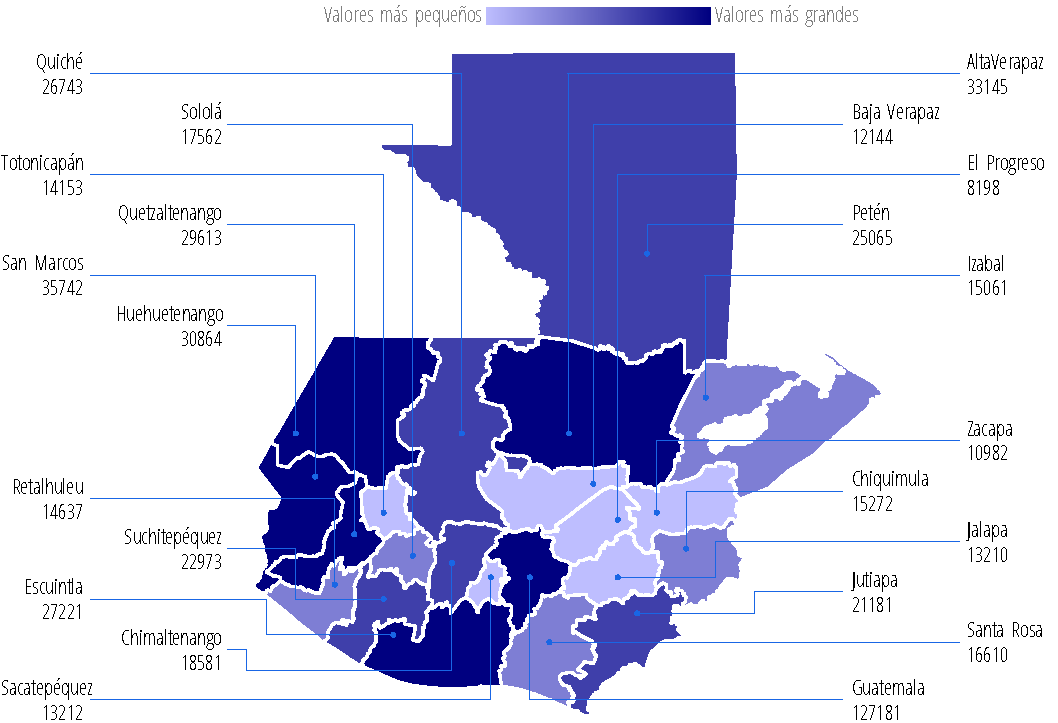
\includegraphics[width=52\cuadri]{graficas/preprimaria/1_6.pdf}}{Instituto Nacional de Estadística, con datos del Ministerio de Educación}




\INEchaptercarta{Indicadores de preprimaria}{}


\cajita{Cobertura bruta}{La tasa bruta de cobertura, establece una relación entre la inscripción inicial total sin distinción de edad, y la población menor de siete años.
	
	En el 2009 la tasa bruta de cobertura en preprimaria fue de 72.1\% y en 2013 fue de 63.5\%, presentando una disminución del 11.9\%.}{Tasa bruta de cobertura del ciclo de educación preprimaria}{República de Guatemala, serie histórica, en porcentaje}{\ \\[0mm]\begin{tikzpicture}[x=1pt,y=1pt]  % Created by tikzDevice version 0.10.1 on 2016-02-29 12:41:28
% !TEX encoding = UTF-8 Unicode
\definecolor{fillColor}{RGB}{255,255,255}
\path[use as bounding box,fill=fillColor,fill opacity=0.00] (0,0) rectangle (289.08,198.74);
\begin{scope}
\path[clip] (  0.00,  0.00) rectangle (289.08,198.74);

\path[] (  0.00,  0.00) rectangle (289.08,198.74);
\end{scope}
\begin{scope}
\path[clip] (  0.00,  0.00) rectangle (289.08,198.74);

\path[] ( -0.52, 15.61) rectangle (280.54,191.48);

\path[] (  0.00, 41.73) --
	(280.54, 41.73);

\path[] (  0.00, 77.99) --
	(280.54, 77.99);

\path[] (  0.00,114.24) --
	(280.54,114.24);

\path[] (  0.00,150.50) --
	(280.54,150.50);

\path[] (  0.00,186.75) --
	(280.54,186.75);

\path[] (  0.00, 23.61) --
	(280.54, 23.61);

\path[] (  0.00, 59.86) --
	(280.54, 59.86);

\path[] (  0.00, 96.12) --
	(280.54, 96.12);

\path[] (  0.00,132.37) --
	(280.54,132.37);

\path[] (  0.00,168.62) --
	(280.54,168.62);

\path[] ( 26.68, 15.61) --
	( 26.68,191.48);

\path[] ( 72.01, 15.61) --
	( 72.01,191.48);

\path[] (117.35, 15.61) --
	(117.35,191.48);

\path[] (162.68, 15.61) --
	(162.68,191.48);

\path[] (208.01, 15.61) --
	(208.01,191.48);

\path[] (253.34, 15.61) --
	(253.34,191.48);
\definecolor{drawColor}{RGB}{0,0,255}

\path[draw=drawColor,line width= 1.7pt,line join=round] ( 26.68,183.49) --
	( 72.01,169.06) --
	(117.35,152.74) --
	(162.68,120.41) --
	(208.01,121.49) --
	(253.34,122.00);
\definecolor{drawColor}{RGB}{0,0,0}

\node[text=drawColor,anchor=base,inner sep=0pt, outer sep=0pt, scale=  1.02] at ( 26.68,187.46) {72.0};

\node[text=drawColor,anchor=base west,inner sep=0pt, outer sep=0pt, scale=  1.02] at ( 72.01,173.03) {70.1};

\node[text=drawColor,anchor=base west,inner sep=0pt, outer sep=0pt, scale=  1.02] at (117.35,156.72) {67.8};

\node[text=drawColor,anchor=base,inner sep=0pt, outer sep=0pt, scale=  1.02] at (162.68,108.49) {63.4};

\node[text=drawColor,anchor=base east,inner sep=0pt, outer sep=0pt, scale=  1.02] at (204.88,121.49) {63.5};

\node[text=drawColor,anchor=base,inner sep=0pt, outer sep=0pt, scale=  1.02] at (253.34,125.97) {63.6};

\path[draw=drawColor,line width= 0.1pt,line join=round] (  0.00, 23.61) -- (280.54, 23.61);

\path[] ( -0.52, 15.61) rectangle (280.54,191.48);
\end{scope}
\begin{scope}
\path[clip] (  0.00,  0.00) rectangle (289.08,198.74);

\path[] (  0.00, 15.61) --
	(280.54, 15.61);
\end{scope}
\begin{scope}
\path[clip] (  0.00,  0.00) rectangle (289.08,198.74);

\path[] ( 26.68, 12.86) --
	( 26.68, 15.61);

\path[] ( 72.01, 12.86) --
	( 72.01, 15.61);

\path[] (117.35, 12.86) --
	(117.35, 15.61);

\path[] (162.68, 12.86) --
	(162.68, 15.61);

\path[] (208.01, 12.86) --
	(208.01, 15.61);

\path[] (253.34, 12.86) --
	(253.34, 15.61);
\end{scope}
\begin{scope}
\path[clip] (  0.00,  0.00) rectangle (289.08,198.74);
\definecolor{drawColor}{RGB}{0,0,0}

\node[text=drawColor,anchor=base,inner sep=0pt, outer sep=0pt, scale=  1.00] at ( 26.68,  2.85) {2009};

\node[text=drawColor,anchor=base,inner sep=0pt, outer sep=0pt, scale=  1.00] at ( 72.01,  2.85) {2010};

\node[text=drawColor,anchor=base,inner sep=0pt, outer sep=0pt, scale=  1.00] at (117.35,  2.85) {2011};

\node[text=drawColor,anchor=base,inner sep=0pt, outer sep=0pt, scale=  1.00] at (162.68,  2.85) {2012};

\node[text=drawColor,anchor=base,inner sep=0pt, outer sep=0pt, scale=  1.00] at (208.01,  2.85) {2013};

\node[text=drawColor,anchor=base,inner sep=0pt, outer sep=0pt, scale=  1.00] at (253.34,  2.85) {2014};
\end{scope}
  \end{tikzpicture}}{Instituto Nacional de Estadística, con datos del Ministerio de Educación}

\cajita{Cobertura bruta por sexo}{La tasa bruta de cobertura en preprimaria fue del 63\% en niños y el 64\% en niñas.}{Tasa bruta de cobertura del ciclo de\\ educación preprimaria, por sexo}{República de Guatemala, año 2013, en porcentaje}{\ \\[0mm]\begin{tikzpicture}[x=1pt,y=1pt]  % Created by tikzDevice version 0.10.1 on 2016-02-29 12:41:34
% !TEX encoding = UTF-8 Unicode
\definecolor{fillColor}{RGB}{255,255,255}
\path[use as bounding box,fill=fillColor,fill opacity=0.00] (0,0) rectangle (289.08,198.74);
\begin{scope}
\path[clip] (  0.00,  0.00) rectangle (289.08,198.74);

\path[] (  0.00,  0.00) rectangle (289.08,198.74);
\end{scope}
\begin{scope}
\path[clip] (  0.00,  0.00) rectangle (289.08,198.74);

\path[] (  0.00, 12.77) rectangle (289.08,181.67);

\path[] ( 54.20, 12.77) --
	( 54.20,181.67);

\path[] (144.54, 12.77) --
	(144.54,181.67);

\path[] (234.88, 12.77) --
	(234.88,181.67);
\definecolor{drawColor}{RGB}{0,0,255}
\definecolor{fillColor}{RGB}{0,0,255}

\path[draw=drawColor,line width= 0.6pt,line join=round,fill=fillColor] ( 36.13, 20.44) rectangle ( 72.27,172.39);

\path[draw=drawColor,line width= 0.6pt,line join=round,fill=fillColor] (126.47, 20.44) rectangle (162.61,170.84);

\path[draw=drawColor,line width= 0.6pt,line join=round,fill=fillColor] (216.81, 20.44) rectangle (252.95,173.99);
\definecolor{drawColor}{RGB}{0,0,0}

\path[draw=drawColor,line width= 0.1pt,line join=round] (  0.00, 20.44) -- (289.08, 20.44);

\node[text=drawColor,anchor=base,inner sep=0pt, outer sep=0pt, scale=  1.02] at ( 54.20,176.36) {63.6};

\node[text=drawColor,anchor=base,inner sep=0pt, outer sep=0pt, scale=  1.02] at (144.54,174.81) {62.9};

\node[text=drawColor,anchor=base,inner sep=0pt, outer sep=0pt, scale=  1.02] at (234.88,177.96) {64.2};

\path[] (  0.00, 12.77) rectangle (289.08,181.67);
\end{scope}
\begin{scope}
\path[clip] (  0.00,  0.00) rectangle (289.08,198.74);

\path[] (  0.00, 12.77) --
	(289.08, 12.77);
\end{scope}
\begin{scope}
\path[clip] (  0.00,  0.00) rectangle (289.08,198.74);

\path[] ( 54.20, 10.02) --
	( 54.20, 12.77);

\path[] (144.54, 10.02) --
	(144.54, 12.77);

\path[] (234.88, 10.02) --
	(234.88, 12.77);
\end{scope}
\begin{scope}
\path[clip] (  0.00,  0.00) rectangle (289.08,198.74);
\definecolor{drawColor}{RGB}{0,0,0}

\node[text=drawColor,anchor=base,inner sep=0pt, outer sep=0pt, scale=  1.00] at ( 54.20, -0.00) {Total};

\node[text=drawColor,anchor=base,inner sep=0pt, outer sep=0pt, scale=  1.00] at (144.54, -0.00) {Hombre};

\node[text=drawColor,anchor=base,inner sep=0pt, outer sep=0pt, scale=  1.00] at (234.88, -0.00) {Mujer};
\end{scope}
  \end{tikzpicture}}{Instituto Nacional de Estadística, con datos del Ministerio de Educación}

\cajota{Cobertura bruta en los departamentos}{Los departamentos que en el 2013 tuvieron la  menor tasa bruta de cobertura en preprimaria fueron: Quiché con el  36.7\%, Totonicapán 41.1\% y Huehuetenango con 42.2\%.
	
	 Los departamentos que tuvieron las más altas tasas brutas de cobertura en preprimaria fueron: Guatemala 93.6\%, El Progreso 95\% y Zacapa  98.5\%.}{Tasa bruta de cobertura del ciclo de educación preprimaria}{Por departamento, año 2013, en porcentaje}{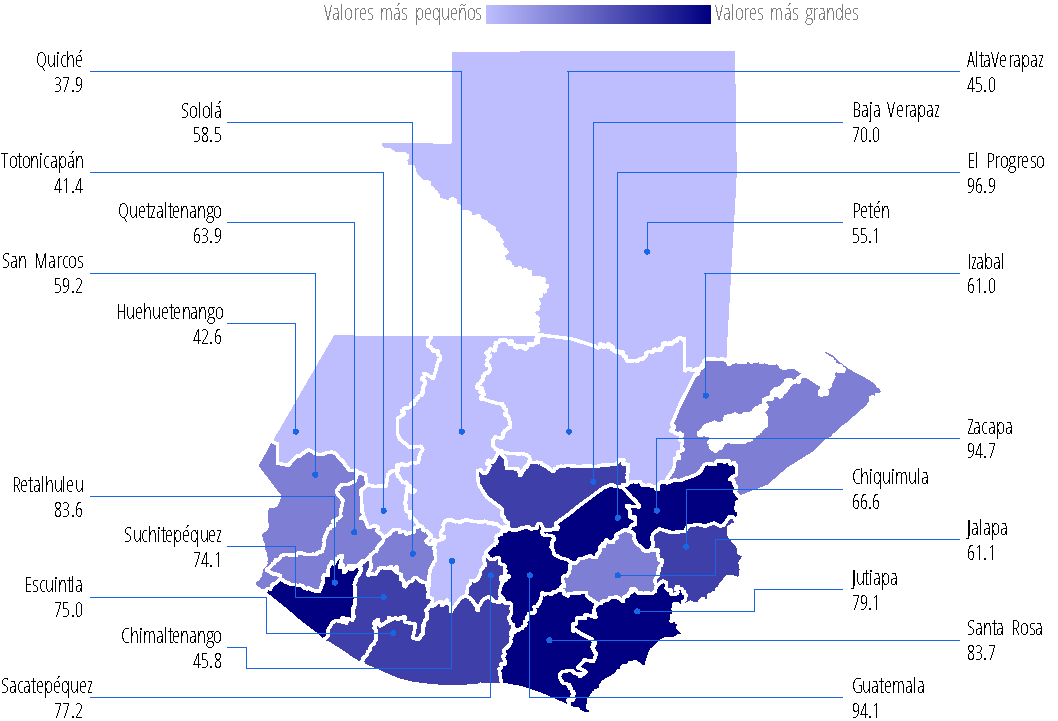
\includegraphics[width=52\cuadri]{graficas/preprimaria/1_9.pdf}}{Instituto Nacional de Estadística, con datos del Ministerio de Educación}

\cajita{Cobertura neta}{ La tasa neta, es la relación que existe entre la parte de la inscripción inicial que se encuentra en la edad escolar hasta de 6 años y la población en edad escolar hasta 6 años.
	
	 En el 2009 la tasa neta de cobertura en preprimaria fue de 57.1\% y en el 2013 fue de 46.2\%,que representa una disminución del 19\%.}{Tasa neta de cobertura del ciclo de educación preprimaria}{República de Guatemala, serie histórica, en porcentaje}{\ \\[0mm]\begin{tikzpicture}[x=1pt,y=1pt]  % Created by tikzDevice version 0.8.1 on 2015-12-10 16:25:47
% !TEX encoding = UTF-8 Unicode
\definecolor{fillColor}{RGB}{255,255,255}
\path[use as bounding box,fill=fillColor,fill opacity=0.00] (0,0) rectangle (289.08,198.74);
\begin{scope}
\path[clip] (  0.00,  0.00) rectangle (289.08,198.74);

\path[] (  0.00,  0.00) rectangle (289.08,198.74);
\end{scope}
\begin{scope}
\path[clip] (  0.00,  0.00) rectangle (289.08,198.74);

\path[] (  1.64, 17.78) rectangle (280.54,191.48);

\path[] (  1.64, 54.82) --
	(280.54, 54.82);

\path[] (  1.64,113.11) --
	(280.54,113.11);

\path[] (  1.64,171.40) --
	(280.54,171.40);

\path[] (  1.64, 25.67) --
	(280.54, 25.67);

\path[] (  1.64, 83.96) --
	(280.54, 83.96);

\path[] (  1.64,142.26) --
	(280.54,142.26);

\path[] ( 28.63, 17.78) --
	( 28.63,191.48);

\path[] ( 73.62, 17.78) --
	( 73.62,191.48);

\path[] (118.60, 17.78) --
	(118.60,191.48);

\path[] (163.59, 17.78) --
	(163.59,191.48);

\path[] (208.57, 17.78) --
	(208.57,191.48);

\path[] (253.55, 17.78) --
	(253.55,191.48);
\definecolor{drawColor}{RGB}{0,0,255}

\path[draw=drawColor,line width= 1.7pt,line join=round] ( 28.63,183.59) --
	( 73.62,170.65) --
	(118.60,128.21) --
	(163.59,112.59) --
	(208.57,120.11) --
	(253.55,126.75);
\definecolor{drawColor}{RGB}{0,0,0}

\node[text=drawColor,anchor=base,inner sep=0pt, outer sep=0pt, scale=  1.01] at ( 28.63,187.54) {57.1};

\node[text=drawColor,anchor=base west,inner sep=0pt, outer sep=0pt, scale=  1.01] at ( 73.62,174.60) {54.9};

\node[text=drawColor,anchor=base west,inner sep=0pt, outer sep=0pt, scale=  1.01] at (118.60,132.17) {47.6};

\node[text=drawColor,anchor=base,inner sep=0pt, outer sep=0pt, scale=  1.01] at (163.59,100.72) {44.9};

\node[text=drawColor,anchor=base east,inner sep=0pt, outer sep=0pt, scale=  1.01] at (205.45,120.11) {46.2};

\node[text=drawColor,anchor=base,inner sep=0pt, outer sep=0pt, scale=  1.01] at (253.55,130.71) {47.3};

\path[draw=drawColor,line width= 0.1pt,line join=round] (  1.64, 25.67) -- (280.54, 25.67);

\path[] (  1.64, 17.78) rectangle (280.54,191.48);
\end{scope}
\begin{scope}
\path[clip] (  0.00,  0.00) rectangle (289.08,198.74);

\path[] (  1.64, 17.78) --
	(  1.64,191.48);
\end{scope}
\begin{scope}
\path[clip] (  0.00,  0.00) rectangle (289.08,198.74);

\path[] (  0.00, 25.67) --
	(  1.64, 25.67);

\path[] (  0.00, 83.96) --
	(  1.64, 83.96);

\path[] (  0.00,142.26) --
	(  1.64,142.26);
\end{scope}
\begin{scope}
\path[clip] (  0.00,  0.00) rectangle (289.08,198.74);

\path[] (  1.64, 17.78) --
	(280.54, 17.78);
\end{scope}
\begin{scope}
\path[clip] (  0.00,  0.00) rectangle (289.08,198.74);

\path[] ( 28.63, 13.51) --
	( 28.63, 17.78);

\path[] ( 73.62, 13.51) --
	( 73.62, 17.78);

\path[] (118.60, 13.51) --
	(118.60, 17.78);

\path[] (163.59, 13.51) --
	(163.59, 17.78);

\path[] (208.57, 13.51) --
	(208.57, 17.78);

\path[] (253.55, 13.51) --
	(253.55, 17.78);
\end{scope}
\begin{scope}
\path[clip] (  0.00,  0.00) rectangle (289.08,198.74);
\definecolor{drawColor}{RGB}{0,0,0}

\node[text=drawColor,anchor=base,inner sep=0pt, outer sep=0pt, scale=  1.00] at ( 28.63,  2.85) {2009};

\node[text=drawColor,anchor=base,inner sep=0pt, outer sep=0pt, scale=  1.00] at ( 73.62,  2.85) {2010};

\node[text=drawColor,anchor=base,inner sep=0pt, outer sep=0pt, scale=  1.00] at (118.60,  2.85) {2011};

\node[text=drawColor,anchor=base,inner sep=0pt, outer sep=0pt, scale=  1.00] at (163.59,  2.85) {2012};

\node[text=drawColor,anchor=base,inner sep=0pt, outer sep=0pt, scale=  1.00] at (208.57,  2.85) {2013};

\node[text=drawColor,anchor=base,inner sep=0pt, outer sep=0pt, scale=  1.00] at (253.55,  2.85) {2014};
\end{scope}
  \end{tikzpicture}}{Instituto Nacional de Estadística, con datos del Ministerio de Educación}

\cajita{Cobertura neta por sexo}{La tasa neta de cobertura en preprimaria por sexo, fue  de 46.1\% en hombres y  46.2\% en mujeres.}{Tasa neta de cobertura del ciclo de educación preprimaria, por sexo}{República de Guatemala, año 2013, en porcentaje}{\ \\[0mm]\begin{tikzpicture}[x=1pt,y=1pt]  % Created by tikzDevice version 0.7.0 on 2015-08-28 13:13:13
% !TEX encoding = UTF-8 Unicode
\definecolor[named]{fillColor}{rgb}{1.00,1.00,1.00}
\path[use as bounding box,fill=fillColor,fill opacity=0.00] (0,0) rectangle (289.08,198.74);
\begin{scope}
\path[clip] (  0.00,  0.00) rectangle (289.08,198.74);
\definecolor[named]{drawColor}{rgb}{1.00,1.00,1.00}

\path[draw=drawColor,line width= 0.6pt,line join=round,line cap=round] (  0.00,  0.00) rectangle (289.08,198.74);
\end{scope}
\begin{scope}
\path[clip] (  0.00,  0.00) rectangle (289.08,198.74);

\path[] (  7.11, 23.47) rectangle (289.08,181.67);

\path[] ( 59.98, 23.47) --
	( 59.98,181.67);

\path[] (148.10, 23.47) --
	(148.10,181.67);

\path[] (236.21, 23.47) --
	(236.21,181.67);
\definecolor[named]{drawColor}{rgb}{0.00,0.00,1.00}
\definecolor[named]{fillColor}{rgb}{0.00,0.00,1.00}

\path[draw=drawColor,line width= 0.6pt,line join=round,fill=fillColor] ( 40.16, 23.47) rectangle ( 79.81,181.67);

\path[draw=drawColor,line width= 0.6pt,line join=round,fill=fillColor] (128.27, 23.47) rectangle (167.92,181.33);

\path[draw=drawColor,line width= 0.6pt,line join=round,fill=fillColor] (216.39, 23.47) rectangle (256.04,181.67);
\definecolor[named]{drawColor}{rgb}{0.00,0.00,0.00}
\definecolor[named]{fillColor}{rgb}{0.00,0.00,0.00}

\path[draw=drawColor,line width= 0.1pt,line join=round,fill=fillColor] (  7.11, 23.47) -- (289.08, 23.47);

\node[text=drawColor,anchor=base,inner sep=0pt, outer sep=0pt, scale=  1.01] at ( 59.98,185.63) {46.2};

\node[text=drawColor,anchor=base,inner sep=0pt, outer sep=0pt, scale=  1.01] at (148.10,185.29) {46.1};

\node[text=drawColor,anchor=base,inner sep=0pt, outer sep=0pt, scale=  1.01] at (236.21,185.63) {46.2};
\end{scope}
\begin{scope}
\path[clip] (  0.00,  0.00) rectangle (289.08,198.74);

\path[] (  7.11, 23.47) --
	(  7.11,181.67);
\end{scope}
\begin{scope}
\path[clip] (  0.00,  0.00) rectangle (289.08,198.74);

\path[] (  7.11, 23.47) --
	(289.08, 23.47);
\end{scope}
\begin{scope}
\path[clip] (  0.00,  0.00) rectangle (289.08,198.74);

\path[] ( 59.98, 19.20) --
	( 59.98, 23.47);

\path[] (148.10, 19.20) --
	(148.10, 23.47);

\path[] (236.21, 19.20) --
	(236.21, 23.47);
\end{scope}
\begin{scope}
\path[clip] (  0.00,  0.00) rectangle (289.08,198.74);
\definecolor[named]{drawColor}{rgb}{0.00,0.00,0.00}

\node[text=drawColor,anchor=base,inner sep=0pt, outer sep=0pt, scale=  1.00] at ( 59.98,  8.54) {Total};

\node[text=drawColor,anchor=base,inner sep=0pt, outer sep=0pt, scale=  1.00] at (148.10,  8.54) {Hombre};

\node[text=drawColor,anchor=base,inner sep=0pt, outer sep=0pt, scale=  1.00] at (236.21,  8.54) {Mujer};
\end{scope}
  \end{tikzpicture}}{Instituto Nacional de Estadística, con datos del Ministerio de Educación}

\cajota{Cobertura neta en los departamentos}{Los departamentos que tuvieron las mas bajas tasas  de cobertura en preprimaria en el 2013 fueron: Quiché 29.4\%, Totonicapán 32.6\% y Alta Verapaz con 34.8\%. 
	
	 Los departamentos que tuvieron las mayores tasas netas de cobertura en preprimaria fueron: Zacapa 59.5\%, El Progreso 59.7\% y Guatemala 66.4\%.}{Tasa neta de cobertura del ciclo de educación preprimaria}{Por departamento, año 2013, en porcentaje}{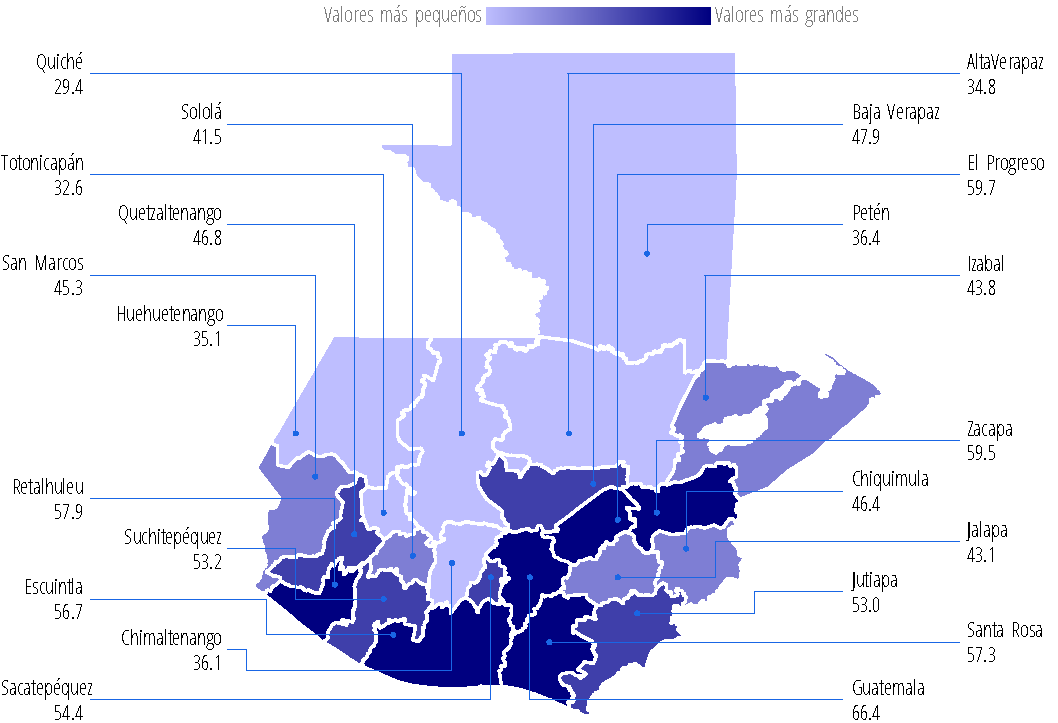
\includegraphics[width=52\cuadri]{graficas/preprimaria/1_12.pdf}}{Instituto Nacional de Estadística, con datos del Ministerio de Educación}



%
%\INEchaptercarta{Alumnos en el nivel primario}{}



\cajita{Inscritos en primaria }{El número de  inscritos en primaria se obtiene a partir del total de los alumnos que tienen hasta doce años, registrados al treinta de marzo de cada año escolar.  
	
En el año 2009 se inscribieron 2,659,776 alumnos y en el 2014 se inscribieron 2,476,379 alumnos, lo cual muestra una disminución de 6.9\%.}{Número de inscritos en el ciclo de educación primaria}{República de Guatemala, serie histórica, en datos absolutos}{\ \\[0mm]}{Instituto Nacional de Estadística, con datos del Ministerio de Educación}

\cajita{Inscritos en primaria por sexo}{En la presente gráfica se observa que el porcentaje de hombres inscritos en primaria es 51.7\% y de mujeres  48.3\% siendo la diferencia de 3.4 puntos porcentuales.}{Distribución de inscritos en el ciclo de educación primaria, por sexo}{República de Guatemala, año 2014, en porcentaje}{\ \\[0mm]}{Instituto Nacional de Estadística, con datos del Ministerio de Educación}

\cajita{Inscritos en primaria por grado}{La presente gráfica desagrega a los inscritos en educación primaria según el grado de estudio.
	
La mayor cantidad de alumnos se concentra en el primer grado, con el 20.3\% y, según esta relación, el 13\% se inscribió en sexto grado.}{Distribución porcentual de inscritos en el ciclo de educación primaria, según el grado escolar}{República de Guatemala, año 2014, en porcentaje}{\ \\[0mm]}{Instituto Nacional de Estadística, con datos del Ministerio de Educación}

\cajita{Inscritos en primaria por etnia}{En la presente gráfica se observa que del total de inscritos en primaria, los no indígenas representan el 61.4\%.}{Distribución de inscritos en el ciclo de educación primaria,\\ por grupo étnico}{República de Guatemala, año 2014, en porcentaje}{\ \\[0mm]}{Instituto Nacional de Estadística, con datos del Ministerio de Educación}


\cajita{Inscritos en primaria por sector educativo}{En la presente gráfica se observa que del total de inscritos en primaria, el 89.2\% están inscritos en el sector público.}{Distribución de inscritos en el ciclo de educación primaria,\\ por sector educativo}{República de Guatemala, año 2014, en porcentaje}{\ \\[0mm]}{Instituto Nacional de Estadística, con datos del Ministerio de Educación}

\cajita{Inscritos en primaria e idioma}{En la gràfica  se observa que del total de inscritos en primaria, el 81.5\% reciben clases en idioma español.}{Distribución de inscritos en el ciclo de educación primaria, según el idioma en el que reciben clases}{República de Guatemala, año 2014, en porcentaje}{\ \\[0mm]}{Instituto Nacional de Estadística, con datos del Ministerio de Educación}

\cajota{Inscritos en primaria en los departamentos}{El mapa muestra en color celeste los departamentos con la menor cantidad de alumnos inscritos, de esta forma los departamentos donde hubo menos alumnos inscritos en primaria fueron: El Progreso 27,212, Zacapa 38,931 y Sacatepéquez 47,012s. 
	
	 Los departamentos con más alumnos inscritos en el 2014 en primaria fueron: Alta Verapaz 212,762, Huehuetenango 214,366  y Guatemala 432,201 alumnos inscritos.}{Inscritos en el ciclo de educación primaria}{Por departamento, año 2014, en datos absolutos}{}{Instituto Nacional de Estadística, con datos del Ministerio de Educación}




\INEchaptercarta[Indicadores de educación primaria]{Indicadores de \\educación primaria}{}


\cajita{Cobertura bruta}{La tasa bruta de cobertura en primaria presentó en el año 2009 el 118.6\% y en el año 2014 fue de 102.7\%, presentando un decrecimiento del 13.5\%.}{Tasa bruta de cobertura del ciclo de educación primaria}{República de Guatemala, serie histórica, en porcentaje}{\ \\[0mm]}{Instituto Nacional de Estadística, con datos del Ministerio de Educación}

\cajita{Cobertura bruta por sexo}{La tasa bruta de cobertura en primaria por sexo, representa 104.8\% para hombres y 100.4\% para mujeres.}{Tasa bruta de cobertura del ciclo de educación primaria, por sexo}{República de Guatemala, año 2014, en porcentaje}{\ \\[0mm]}{Instituto Nacional de Estadística, con datos del Ministerio de Educación}

\cajota{Cobertura bruta en los departamentos}{El mapa muestra en color celeste los departamentos con las menores tasas brutas de cobertura en primaria, que fueron: Petén 85.7\%, Chimaltenango 90\% y Totonicapán con 90.3\%. 
	
	 Los departamentos con las más altas tassa bruta de cobertura en primaria en el 2014, fueron: Santa Rosa 112.3\%, San Marcos 112.6\% y Retalhuleu 113.4\%. El departamento de Guatemala presentó una tasa de 103.8\%.}{Tasa bruta de cobertura del ciclo de educación primaria}{Por departamento, año 2014, en porcentaje}{}{Instituto Nacional de Estadística, con datos del Ministerio de Educación}

\cajita{Cobertura neta}{La tasa neta de cobertura en primaria presentó el año 2009 el 98.7\% y en el año 2014 fue de 85.4\%, presentando un decrecimiento del 13.5\%.}{Tasa neta de cobertura del ciclo de educación primaria}{República de Guatemala, serie histórica, en porcentaje}{\ \\[0mm]}{Instituto Nacional de Estadística, con datos del Ministerio de Educación}

\cajita{Cobertura neta por sexo}{La tasa neta de cobertura en primaria por sexo, representa el 86\% para hombres y 84.8\% para las mujeres.}{Tasa neta de cobertura del ciclo de educación primaria, por sexo}{República de Guatemala, año 2014, en porcentaje}{\ \\[0mm]}{Instituto Nacional de Estadística, con datos del Ministerio de Educación}

\cajota{Cobertura neta en los departamentos}{El mapa muestra en color celeste los departamentos con las menores tasas netas de cobertura en primaria, que fueron: Petén 68.0\%, Totonicapán 74.2\% y Sololá 75.9.  
	
	Los departamentos donde hubo alta tasa neta de cobertura en primaria fueron: Zacapa 93.2\%, Retalhuleu 93.6 y San Marcos 93.8\% .El departamento de Guatemala presentó una tasa de  91.3\%. }{Tasa neta de cobertura del ciclo de educación primaria}{Por departamento, año 2014, en porcentaje}{}{Instituto Nacional de Estadística, con datos del Ministerio de Educación}




\cajita{Repitencia}{La tasa de repitencia en primaria es la relación que existe entre el número de repitentes y el número de alumnos que en el año  estaban inscritos en el mismo grado.
	
	En el año 2009 fue del 11.5\% y en el 2014 fue de 10.2\%, presentando un decrecimiento del 11.3\%.}{Tasa de repitencia del ciclo de educación primaria}{República de Guatemala, serie histórica, en porcentaje}{\ \\[0mm]}{Instituto Nacional de Estadística, con datos del Ministerio de Educación}

\cajita{Repitencia por sexo}{La tasa de repitencia en primaria por sexo, representa el 11.2\% para hombres y 9.2\% para las mujeres.}{Tasa de repitencia del ciclo de educación primaria, por sexo}{República de Guatemala, año 2014, en porcentaje}{\ \\[0mm]}{Instituto Nacional de Estadística, con datos del Ministerio de Educación}

\cajota{Repitencia en los departamentos}{El mapa muestra en color celeste los departamentos con las menores tasas de repitencia en primaria, que fueron: Guatemala 4.6\%, Jutiapa 7.3\% y Retalhuleu 7.4 \%.  
	
	Los departamentos con las mayores tasas  de repitencia en primaria: Jalapa 13.5\%, Quiché 13.7\% y Alta Verapaz con 16.5\%.}{Tasa de repitencia del ciclo de educación primaria}{Por departamento, año 2014, en porcentaje}{}{Instituto Nacional de Estadística, con datos del Ministerio de Educación}






\cajita{Sobre-edad}{La tasa de  sobre-edad , es la relación que existe entre la cantidad de alumnos inscritos en los diferentes grados de un nivel educativo, con dos o más años de atraso escolar por encima de la edad correspondiente al grado de estudio. 
	
	En el año 2009 fue del 51.7\% y en el año 2014 fue de 20.8\%, presentando un decrecimiento del 59.8\%.}{Tasa de sobre-edad del ciclo de educación primaria}{República de Guatemala, serie histórica, en porcentaje}{\ \\[0mm]}{Instituto Nacional de Estadística, con datos del Ministerio de Educación}

\cajita{Sobre-edad por sexo}{La tasa de  sobre-edad en primaria por sexo, representa el 22.7\% para hombres y 18.7\% para las mujeres.}{Tasa de sobre-edad del ciclo de educación primaria, por sexo}{República de Guatemala, año 2014, en porcentaje}{\ \\[0mm]}{Instituto Nacional de Estadística, con datos del Ministerio de Educación}

\cajota{Sobre-edad en los departamentos}{El mapa muestra en color celeste los departamentos con las menores tasas de sobre-edad en primaria en el 2014, que fueron: Guatemala 10.7\%, Sacatepéquez 12.5\% y Chimaltenango 15.1\%. 
	
	 Los departamentos con las mayores tasas  de sobre-edad en primaria: Quiché 27.0\% Petén 28.9\% y Alta Verapaz 30.9\%.}{Tasa de sobre-edad del ciclo de educación primaria}{Por departamento, año 2014, en porcentaje}{}{Instituto Nacional de Estadística, con datos del Ministerio de Educación}





\cajita{Deserción}{La tasa de deserción en primaria , se refiere a la cantidad de alumnos que no concluyen el ciclo lectivo. 
	
	En el año 2009 fue de 5.5\% y en el año 2014 fue de 3.5\%, presentando un decrecimiento de 3.5\%.}{Tasa de deserción del ciclo de educación primaria}{República de Guatemala, serie histórica, en porcentaje}{\ \\[0mm]}{Instituto Nacional de Estadística, con datos del Ministerio de Educación}

\cajita{Deserción por sexo}{La tasa de deserción en primaria por sexo, representa el 3.8\% para hombres y 3.1\% para las mujeres.}{Tasa de deserción del ciclo de educación primaria, por sexo}{República de Guatemala, año 2014, en porcentaje}{\ \\[0mm]}{Instituto Nacional de Estadística, con datos del Ministerio de Educación}

\cajota{Deserción en los departamentos}{El mapa muestra en color celeste los departamentos con las menores tasas de deserción en primaria: Chimaltenango 1.8\%, Quiché 1.9\% y Sacatepéquez 2\%. 
	
	 Los departamentos con las mayores tasas de deserción en primaria en el 2014, fueron: Izabal 6.6\%, Retalhuleu 6.6 y Petén 7.2\%. En el departamento de Guatemala la tasa de deserción fue de 2.5\%.	}{Tasa de deserción del ciclo de educación primaria}{Por departamento, año 2014, en porcentaje}{}{Instituto Nacional de Estadística, con datos del Ministerio de Educación}




\cajita{Aprobación}{La tasa de aprobación en primaria se refiere a la cantidad de alumnos que culminaron y aprobaron el ciclo lectivo.
	
	En el año 2009 fue de 86.4\% y en el año 2014 fue de 86.6\%, presentando un crecimiento de 0.2\%.}{Tasa de aprobación del ciclo de educación primaria}{República de Guatemala, serie histórica, en porcentaje}{\ \\[0mm]}{Instituto Nacional de Estadística, con datos del Ministerio de Educación}

\cajita{Aprobación por sexo}{La tasa de aprobación en primaria por sexo, representa el 85.3\% para hombres y 87.9\% para las mujeres.}{Tasa de aprobación del ciclo de educación primaria, por sexo}{República de Guatemala, año 2014, en porcentaje}{\ \\[0mm]}{Instituto Nacional de Estadística, con datos del Ministerio de Educación}

\cajota{Aprobación en los departamentos}{El mapa muestra en color celeste los departamentos con las menores tasas de aprobación en primaria: Alta Verapaz 77.1\%, Chiquimula 81.3\% y Quiché 81.8\%.
	
	  Los departamentos con las mayores tasas  de aprobación en primaria fueron: Retalhuleu 88.9\%, Sacatepéquez 89.9\% y Guatemala 93.7\%. }{Tasa de aprobación del ciclo de educación primaria}{Por departamento, año 2014, en porcentaje}{}{Instituto Nacional de Estadística, con datos del Ministerio de Educación}




%
%
%\INEchaptercarta{Alumnos en el ciclo básico}{}



\cajita{Inscritos en básicos }{El número de  inscritos en básicos se obtiene a partir del total de los alumnos registrados al treinta de marzo de cada año escolar, sin distinción de la edad y que se matriculan en el ciclo básico.
	
	 En el año 2009 se inscribieron 671,872 alumnos y en el 2014 se inscribieron 769,163, lo cual muestra un crecimiento de 14.5\%.}{Número de inscritos en el ciclo de educación básica}{República de Guatemala, serie histórica, en datos absolutos}{\ \\[0mm]\begin{tikzpicture}[x=1pt,y=1pt]  % Created by tikzDevice version 0.7.0 on 2015-08-28 13:08:39
% !TEX encoding = UTF-8 Unicode
\definecolor[named]{fillColor}{rgb}{1.00,1.00,1.00}
\path[use as bounding box,fill=fillColor,fill opacity=0.00] (0,0) rectangle (289.08,198.74);
\begin{scope}
\path[clip] (  0.00,  0.00) rectangle (289.08,198.74);
\definecolor[named]{drawColor}{rgb}{1.00,1.00,1.00}

\path[draw=drawColor,line width= 0.6pt,line join=round,line cap=round] (  0.00,  0.00) rectangle (289.08,198.74);
\end{scope}
\begin{scope}
\path[clip] (  0.00,  0.00) rectangle (289.08,198.74);

\path[] ( 14.70, 17.78) rectangle (280.54,191.48);

\path[] ( 14.70, 46.32) --
	(280.54, 46.32);

\path[] ( 14.70, 87.64) --
	(280.54, 87.64);

\path[] ( 14.70,128.96) --
	(280.54,128.96);

\path[] ( 14.70,170.28) --
	(280.54,170.28);

\path[] ( 14.70, 25.66) --
	(280.54, 25.66);

\path[] ( 14.70, 66.98) --
	(280.54, 66.98);

\path[] ( 14.70,108.30) --
	(280.54,108.30);

\path[] ( 14.70,149.62) --
	(280.54,149.62);

\path[] ( 14.70,190.94) --
	(280.54,190.94);

\path[] ( 45.37, 17.78) --
	( 45.37,191.48);

\path[] ( 96.50, 17.78) --
	( 96.50,191.48);

\path[] (147.62, 17.78) --
	(147.62,191.48);

\path[] (198.74, 17.78) --
	(198.74,191.48);

\path[] (249.87, 17.78) --
	(249.87,191.48);
\definecolor[named]{drawColor}{rgb}{0.00,0.00,1.00}

\path[draw=drawColor,line width= 1.7pt,line join=round] ( 45.37,164.47) --
	( 96.50,176.67) --
	(147.62,178.72) --
	(198.74,179.89) --
	(249.87,183.59);
\definecolor[named]{drawColor}{rgb}{0.00,0.00,0.00}

\node[text=drawColor,anchor=base,inner sep=0pt, outer sep=0pt, scale=  1.01] at ( 45.37,152.60) {671,872};

\node[text=drawColor,anchor=base east,inner sep=0pt, outer sep=0pt, scale=  1.01] at ( 90.72,176.67) {730,929};

\node[text=drawColor,anchor=base east,inner sep=0pt, outer sep=0pt, scale=  1.01] at (141.84,183.72) {740,877};

\node[text=drawColor,anchor=base east,inner sep=0pt, outer sep=0pt, scale=  1.01] at (192.97,183.89) {746,516};

\node[text=drawColor,anchor=base,inner sep=0pt, outer sep=0pt, scale=  1.01] at (249.87,187.54) {764,415};
\definecolor[named]{fillColor}{rgb}{0.00,0.00,0.00}

\path[draw=drawColor,line width= 0.1pt,line join=round,fill=fillColor] ( 14.70, 25.67) -- (280.54, 25.67);
\end{scope}
\begin{scope}
\path[clip] (  0.00,  0.00) rectangle (289.08,198.74);

\path[] ( 14.70, 17.78) --
	( 14.70,191.48);
\end{scope}
\begin{scope}
\path[clip] (  0.00,  0.00) rectangle (289.08,198.74);
\definecolor[named]{drawColor}{rgb}{1.00,1.00,1.00}

\node[text=drawColor,text opacity=0.00,anchor=base east,inner sep=0pt, outer sep=0pt, scale=  1.00] at (  7.58, 21.75) {0e+00};

\node[text=drawColor,text opacity=0.00,anchor=base east,inner sep=0pt, outer sep=0pt, scale=  1.00] at (  7.58, 63.07) {2e+05};

\node[text=drawColor,text opacity=0.00,anchor=base east,inner sep=0pt, outer sep=0pt, scale=  1.00] at (  7.58,104.39) {4e+05};

\node[text=drawColor,text opacity=0.00,anchor=base east,inner sep=0pt, outer sep=0pt, scale=  1.00] at (  7.58,145.71) {6e+05};

\node[text=drawColor,text opacity=0.00,anchor=base east,inner sep=0pt, outer sep=0pt, scale=  1.00] at (  7.58,187.03) {8e+05};
\end{scope}
\begin{scope}
\path[clip] (  0.00,  0.00) rectangle (289.08,198.74);

\path[] ( 10.43, 25.66) --
	( 14.70, 25.66);

\path[] ( 10.43, 66.98) --
	( 14.70, 66.98);

\path[] ( 10.43,108.30) --
	( 14.70,108.30);

\path[] ( 10.43,149.62) --
	( 14.70,149.62);

\path[] ( 10.43,190.94) --
	( 14.70,190.94);
\end{scope}
\begin{scope}
\path[clip] (  0.00,  0.00) rectangle (289.08,198.74);

\path[] ( 14.70, 17.78) --
	(280.54, 17.78);
\end{scope}
\begin{scope}
\path[clip] (  0.00,  0.00) rectangle (289.08,198.74);

\path[] ( 45.37, 13.51) --
	( 45.37, 17.78);

\path[] ( 96.50, 13.51) --
	( 96.50, 17.78);

\path[] (147.62, 13.51) --
	(147.62, 17.78);

\path[] (198.74, 13.51) --
	(198.74, 17.78);

\path[] (249.87, 13.51) --
	(249.87, 17.78);
\end{scope}
\begin{scope}
\path[clip] (  0.00,  0.00) rectangle (289.08,198.74);
\definecolor[named]{drawColor}{rgb}{0.00,0.00,0.00}

\node[text=drawColor,anchor=base,inner sep=0pt, outer sep=0pt, scale=  1.00] at ( 45.37,  2.85) {2009};

\node[text=drawColor,anchor=base,inner sep=0pt, outer sep=0pt, scale=  1.00] at ( 96.50,  2.85) {2010};

\node[text=drawColor,anchor=base,inner sep=0pt, outer sep=0pt, scale=  1.00] at (147.62,  2.85) {2011};

\node[text=drawColor,anchor=base,inner sep=0pt, outer sep=0pt, scale=  1.00] at (198.74,  2.85) {2012};

\node[text=drawColor,anchor=base,inner sep=0pt, outer sep=0pt, scale=  1.00] at (249.87,  2.85) {2014};
\end{scope}
  \end{tikzpicture}}{Instituto Nacional de Estadística, con datos del Ministerio de Educación}

\cajita{Inscritos en básicos por sexo}{La distribución por sexo de los alumnos inscritos en educación básica muestra que el 53.4\% fueron hombres y de mujeres  46.6\%.}{Distribución de inscritos en el ciclo de educación básica, por sexo}{República de Guatemala, año 2014, en porcentaje}{\ \\[0mm]\begin{tikzpicture}[x=1pt,y=1pt]  % Created by tikzDevice version 0.10.1 on 2016-02-29 12:50:32
% !TEX encoding = UTF-8 Unicode
\definecolor{fillColor}{RGB}{255,255,255}
\path[use as bounding box,fill=fillColor,fill opacity=0.00] (0,0) rectangle (289.08,198.74);
\begin{scope}
\path[clip] ( 30.54,  0.00) rectangle (258.54,198.74);

\path[] ( 30.54,  0.00) rectangle (258.54,198.74);
\end{scope}
\begin{scope}
\path[clip] (  0.00,  0.00) rectangle (289.08,198.74);

\path[] (  7.11,  4.95) rectangle (200.91,198.74);

\path[] (104.01,101.85) --
	(190.71, 92.51);

\path[] (104.01,101.85) --
	( 17.30,111.18);

\path[] (104.01,101.85) --
	(113.34,188.55);

\path[] (104.01,101.85) --
	(190.71, 92.51);

\path[] (104.01,101.85) --
	( 94.67, 15.14);

\path[] (104.01,101.85) --
	( 17.30,111.18);

\path[] (104.01,101.85) --
	(104.01,101.85) --
	(104.01,101.85) --
	(104.01,101.85) --
	(104.01,101.85) --
	(104.01,101.85) --
	(104.01,101.85) --
	(104.01,101.85) --
	(104.01,101.85) --
	(104.01,101.85) --
	(104.01,101.85) --
	(104.01,101.85) --
	(104.01,101.85) --
	(104.01,101.85) --
	(104.01,101.85) --
	(104.01,101.85) --
	(104.01,101.85) --
	(104.01,101.85) --
	(104.01,101.85) --
	(104.01,101.85) --
	(104.01,101.85) --
	(104.01,101.85) --
	(104.01,101.85) --
	(104.01,101.85) --
	(104.01,101.85) --
	(104.01,101.85) --
	(104.01,101.85) --
	(104.01,101.85) --
	(104.01,101.85) --
	(104.01,101.85) --
	(104.01,101.85) --
	(104.01,101.85) --
	(104.01,101.85) --
	(104.01,101.85) --
	(104.01,101.85) --
	(104.01,101.85) --
	(104.01,101.85) --
	(104.01,101.85) --
	(104.01,101.85) --
	(104.01,101.85) --
	(104.01,101.85) --
	(104.01,101.85) --
	(104.01,101.85) --
	(104.01,101.85) --
	(104.01,101.85) --
	(104.01,101.85) --
	(104.01,101.85) --
	(104.01,101.85) --
	(104.01,101.85) --
	(104.01,101.85) --
	(104.01,101.85) --
	(104.01,101.85) --
	(104.01,101.85) --
	(104.01,101.85) --
	(104.01,101.85) --
	(104.01,101.85) --
	(104.01,101.85) --
	(104.01,101.85) --
	(104.01,101.85) --
	(104.01,101.85) --
	(104.01,101.85) --
	(104.01,101.85) --
	(104.01,101.85) --
	(104.01,101.85) --
	(104.01,101.85) --
	(104.01,101.85) --
	(104.01,101.85) --
	(104.01,101.85) --
	(104.01,101.85) --
	(104.01,101.85) --
	(104.01,101.85) --
	(104.01,101.85) --
	(104.01,101.85) --
	(104.01,101.85) --
	(104.01,101.85) --
	(104.01,101.85) --
	(104.01,101.85) --
	(104.01,101.85) --
	(104.01,101.85) --
	(104.01,101.85) --
	(104.01,101.85) --
	(104.01,101.85) --
	(104.01,101.85) --
	(104.01,101.85) --
	(104.01,101.85) --
	(104.01,101.85) --
	(104.01,101.85) --
	(104.01,101.85) --
	(104.01,101.85) --
	(104.01,101.85) --
	(104.01,101.85) --
	(104.01,101.85) --
	(104.01,101.85) --
	(104.01,101.85) --
	(104.01,101.85) --
	(104.01,101.85) --
	(104.01,101.85) --
	(104.01,101.85) --
	(104.01,101.85) --
	(104.01,101.85);

\path[] (104.01,121.23) --
	(105.24,121.19) --
	(106.46,121.07) --
	(107.68,120.88) --
	(108.88,120.60) --
	(110.06,120.26) --
	(111.21,119.84) --
	(112.34,119.34) --
	(113.43,118.78) --
	(114.49,118.15) --
	(115.50,117.45) --
	(116.47,116.69) --
	(117.38,115.87) --
	(118.25,115.00) --
	(119.05,114.07) --
	(119.80,113.09) --
	(120.48,112.06) --
	(121.09,111.00) --
	(121.64,109.90) --
	(122.11,108.76) --
	(122.51,107.60) --
	(122.84,106.42) --
	(123.09,105.21) --
	(123.27,103.99) --
	(123.37,102.77) --
	(123.39,101.54) --
	(123.33,100.31) --
	(123.19, 99.09) --
	(122.98, 97.88) --
	(122.69, 96.68) --
	(122.32, 95.51) --
	(121.88, 94.36) --
	(121.37, 93.24) --
	(120.79, 92.16) --
	(120.14, 91.11) --
	(119.43, 90.11) --
	(118.66, 89.16) --
	(117.82, 88.25) --
	(116.93, 87.40) --
	(115.99, 86.61) --
	(115.00, 85.88) --
	(113.96, 85.22) --
	(112.89, 84.62) --
	(111.78, 84.09) --
	(110.64, 83.64) --
	(109.47, 83.25) --
	(108.28, 82.94) --
	(107.07, 82.71) --
	(105.85, 82.55) --
	(104.62, 82.48) --
	(103.39, 82.48) --
	(102.17, 82.55) --
	(100.95, 82.71) --
	( 99.74, 82.94) --
	( 98.55, 83.25) --
	( 97.38, 83.64) --
	( 96.24, 84.09) --
	( 95.13, 84.62) --
	( 94.05, 85.22) --
	( 93.02, 85.88) --
	( 92.03, 86.61) --
	( 91.09, 87.40) --
	( 90.20, 88.25) --
	( 89.36, 89.16) --
	( 88.59, 90.11) --
	( 87.87, 91.11) --
	( 87.23, 92.16) --
	( 86.65, 93.24) --
	( 86.13, 94.36) --
	( 85.70, 95.51) --
	( 85.33, 96.68) --
	( 85.04, 97.88) --
	( 84.83, 99.09) --
	( 84.69,100.31) --
	( 84.63,101.54) --
	( 84.65,102.77) --
	( 84.75,103.99) --
	( 84.92,105.21) --
	( 85.18,106.42) --
	( 85.50,107.60) --
	( 85.91,108.76) --
	( 86.38,109.90) --
	( 86.93,111.00) --
	( 87.54,112.06) --
	( 88.22,113.09) --
	( 88.97,114.07) --
	( 89.77,115.00) --
	( 90.64,115.87) --
	( 91.55,116.69) --
	( 92.52,117.45) --
	( 93.53,118.15) --
	( 94.59,118.78) --
	( 95.68,119.34) --
	( 96.81,119.84) --
	( 97.96,120.26) --
	( 99.14,120.60) --
	(100.34,120.88) --
	(101.56,121.07) --
	(102.78,121.19) --
	(104.01,121.23);

\path[] (104.01,140.60) --
	(106.47,140.53) --
	(108.92,140.29) --
	(111.34,139.90) --
	(113.74,139.36) --
	(116.10,138.67) --
	(118.41,137.83) --
	(120.67,136.84) --
	(122.85,135.72) --
	(124.96,134.45) --
	(126.99,133.06) --
	(128.92,131.54) --
	(130.76,129.90) --
	(132.48,128.14) --
	(134.09,126.29) --
	(135.58,124.33) --
	(136.94,122.28) --
	(138.17,120.15) --
	(139.27,117.95) --
	(140.22,115.68) --
	(141.02,113.35) --
	(141.68,110.98) --
	(142.18,108.58) --
	(142.53,106.14) --
	(142.72,103.69) --
	(142.76,101.23) --
	(142.65, 98.77) --
	(142.37, 96.33) --
	(141.95, 93.91) --
	(141.37, 91.52) --
	(140.64, 89.17) --
	(139.76, 86.87) --
	(138.74, 84.63) --
	(137.58, 82.47) --
	(136.28, 80.38) --
	(134.85, 78.37) --
	(133.30, 76.46) --
	(131.63, 74.66) --
	(129.85, 72.96) --
	(127.97, 71.38) --
	(125.99, 69.92) --
	(123.92, 68.59) --
	(121.77, 67.40) --
	(119.55, 66.34) --
	(117.27, 65.43) --
	(114.93, 64.66) --
	(112.55, 64.04) --
	(110.13, 63.57) --
	(107.69, 63.26) --
	(105.24, 63.11) --
	(102.78, 63.11) --
	(100.33, 63.26) --
	( 97.89, 63.57) --
	( 95.47, 64.04) --
	( 93.09, 64.66) --
	( 90.75, 65.43) --
	( 88.47, 66.34) --
	( 86.25, 67.40) --
	( 84.10, 68.59) --
	( 82.03, 69.92) --
	( 80.05, 71.38) --
	( 78.17, 72.96) --
	( 76.39, 74.66) --
	( 74.72, 76.46) --
	( 73.17, 78.37) --
	( 71.74, 80.38) --
	( 70.44, 82.47) --
	( 69.28, 84.63) --
	( 68.26, 86.87) --
	( 67.38, 89.17) --
	( 66.65, 91.52) --
	( 66.07, 93.91) --
	( 65.65, 96.33) --
	( 65.37, 98.77) --
	( 65.26,101.23) --
	( 65.29,103.69) --
	( 65.49,106.14) --
	( 65.84,108.58) --
	( 66.34,110.98) --
	( 67.00,113.35) --
	( 67.80,115.68) --
	( 68.75,117.95) --
	( 69.85,120.15) --
	( 71.08,122.28) --
	( 72.44,124.33) --
	( 73.93,126.29) --
	( 75.54,128.14) --
	( 77.26,129.90) --
	( 79.10,131.54) --
	( 81.03,133.06) --
	( 83.06,134.45) --
	( 85.17,135.72) --
	( 87.35,136.84) --
	( 89.60,137.83) --
	( 91.92,138.67) --
	( 94.28,139.36) --
	( 96.67,139.90) --
	( 99.10,140.29) --
	(101.55,140.53) --
	(104.01,140.60);

\path[] (104.01,159.98) --
	(107.70,159.87) --
	(111.37,159.52) --
	(115.01,158.93) --
	(118.61,158.12) --
	(122.15,157.08) --
	(125.62,155.82) --
	(129.00,154.34) --
	(132.28,152.65) --
	(135.44,150.75) --
	(138.48,148.66) --
	(141.38,146.38) --
	(144.13,143.92) --
	(146.72,141.29) --
	(149.13,138.51) --
	(151.37,135.57) --
	(153.41,132.50) --
	(155.26,129.30) --
	(156.89,126.00) --
	(158.32,122.59) --
	(159.53,119.11) --
	(160.51,115.55) --
	(161.26,111.94) --
	(161.79,108.29) --
	(162.08,104.61) --
	(162.14,100.92) --
	(161.96, 97.24) --
	(161.56, 93.57) --
	(160.91, 89.94) --
	(160.05, 86.35) --
	(158.95, 82.83) --
	(157.63, 79.39) --
	(156.10, 76.03) --
	(154.36, 72.78) --
	(152.41, 69.64) --
	(150.27, 66.64) --
	(147.95, 63.77) --
	(145.44, 61.06) --
	(142.77, 58.52) --
	(139.95, 56.15) --
	(136.98, 53.96) --
	(133.87, 51.97) --
	(130.65, 50.17) --
	(127.32, 48.59) --
	(123.89, 47.21) --
	(120.39, 46.06) --
	(116.82, 45.14) --
	(113.20, 44.44) --
	(109.54, 43.97) --
	(105.85, 43.74) --
	(102.16, 43.74) --
	( 98.48, 43.97) --
	( 94.82, 44.44) --
	( 91.20, 45.14) --
	( 87.63, 46.06) --
	( 84.13, 47.21) --
	( 80.70, 48.59) --
	( 77.37, 50.17) --
	( 74.15, 51.97) --
	( 71.04, 53.96) --
	( 68.07, 56.15) --
	( 65.25, 58.52) --
	( 62.58, 61.06) --
	( 60.07, 63.77) --
	( 57.75, 66.64) --
	( 55.61, 69.64) --
	( 53.66, 72.78) --
	( 51.92, 76.03) --
	( 50.39, 79.39) --
	( 49.07, 82.83) --
	( 47.97, 86.35) --
	( 47.10, 89.94) --
	( 46.46, 93.57) --
	( 46.05, 97.24) --
	( 45.88,100.92) --
	( 45.94,104.61) --
	( 46.23,108.29) --
	( 46.75,111.94) --
	( 47.51,115.55) --
	( 48.49,119.11) --
	( 49.70,122.59) --
	( 51.13,126.00) --
	( 52.76,129.30) --
	( 54.61,132.50) --
	( 56.65,135.57) --
	( 58.89,138.51) --
	( 61.30,141.29) --
	( 63.89,143.92) --
	( 66.64,146.38) --
	( 69.54,148.66) --
	( 72.58,150.75) --
	( 75.74,152.65) --
	( 79.02,154.34) --
	( 82.40,155.82) --
	( 85.87,157.08) --
	( 89.41,158.12) --
	( 93.01,158.93) --
	( 96.65,159.52) --
	(100.32,159.87) --
	(104.01,159.98);

\path[] (104.01,179.36) --
	(108.93,179.21) --
	(113.82,178.74) --
	(118.68,177.96) --
	(123.48,176.88) --
	(128.20,175.49) --
	(132.82,173.81) --
	(137.33,171.84) --
	(141.70,169.58) --
	(145.92,167.06) --
	(149.97,164.27) --
	(153.84,161.23) --
	(157.50,157.95) --
	(160.95,154.44) --
	(164.17,150.72) --
	(167.15,146.81) --
	(169.88,142.72) --
	(172.34,138.46) --
	(174.52,134.05) --
	(176.42,129.51) --
	(178.03,124.86) --
	(179.34,120.12) --
	(180.35,115.31) --
	(181.05,110.44) --
	(181.44,105.53) --
	(181.52,100.62) --
	(181.28, 95.70) --
	(180.74, 90.81) --
	(179.88, 85.97) --
	(178.72, 81.19) --
	(177.26, 76.49) --
	(175.51, 71.90) --
	(173.46, 67.42) --
	(171.14, 63.09) --
	(168.55, 58.91) --
	(165.69, 54.90) --
	(162.59, 51.08) --
	(159.26, 47.47) --
	(155.70, 44.08) --
	(151.93, 40.91) --
	(147.97, 38.00) --
	(143.83, 35.34) --
	(139.53, 32.95) --
	(135.09, 30.83) --
	(130.52, 29.00) --
	(125.85, 27.47) --
	(121.09, 26.23) --
	(116.26, 25.30) --
	(111.38, 24.68) --
	(106.47, 24.37) --
	(101.55, 24.37) --
	( 96.64, 24.68) --
	( 91.76, 25.30) --
	( 86.93, 26.23) --
	( 82.17, 27.47) --
	( 77.50, 29.00) --
	( 72.93, 30.83) --
	( 68.49, 32.95) --
	( 64.19, 35.34) --
	( 60.05, 38.00) --
	( 56.09, 40.91) --
	( 52.32, 44.08) --
	( 48.76, 47.47) --
	( 45.43, 51.08) --
	( 42.32, 54.90) --
	( 39.47, 58.91) --
	( 36.88, 63.09) --
	( 34.55, 67.42) --
	( 32.51, 71.90) --
	( 30.76, 76.49) --
	( 29.30, 81.19) --
	( 28.14, 85.97) --
	( 27.28, 90.81) --
	( 26.74, 95.70) --
	( 26.50,100.62) --
	( 26.58,105.53) --
	( 26.97,110.44) --
	( 27.67,115.31) --
	( 28.68,120.12) --
	( 29.99,124.86) --
	( 31.60,129.51) --
	( 33.50,134.05) --
	( 35.68,138.46) --
	( 38.14,142.72) --
	( 40.87,146.81) --
	( 43.84,150.72) --
	( 47.07,154.44) --
	( 50.52,157.95) --
	( 54.18,161.23) --
	( 58.05,164.27) --
	( 62.10,167.06) --
	( 66.32,169.58) --
	( 70.69,171.84) --
	( 75.20,173.81) --
	( 79.82,175.49) --
	( 84.54,176.88) --
	( 89.34,177.96) --
	( 94.20,178.74) --
	( 99.09,179.21) --
	(104.01,179.36);

\path[] (104.01,189.05) --
	(109.54,188.88) --
	(115.05,188.35) --
	(120.51,187.48) --
	(125.91,186.26) --
	(131.22,184.70) --
	(136.42,182.81) --
	(141.49,180.59) --
	(146.41,178.05) --
	(151.16,175.21) --
	(155.71,172.07) --
	(160.06,168.65) --
	(164.19,164.96) --
	(168.07,161.02) --
	(171.69,156.83) --
	(175.05,152.43) --
	(178.11,147.82) --
	(180.88,143.03) --
	(183.34,138.07) --
	(185.47,132.97) --
	(187.28,127.74) --
	(188.76,122.41) --
	(189.89,116.99) --
	(190.68,111.51) --
	(191.12,106.00) --
	(191.21,100.46) --
	(190.94, 94.94) --
	(190.33, 89.44) --
	(189.37, 83.99) --
	(188.06, 78.61) --
	(186.42, 73.32) --
	(184.44, 68.15) --
	(182.15, 63.12) --
	(179.53, 58.24) --
	(176.62, 53.54) --
	(173.41, 49.03) --
	(169.92, 44.74) --
	(166.16, 40.67) --
	(162.16, 36.85) --
	(157.92, 33.30) --
	(153.46, 30.02) --
	(148.81, 27.02) --
	(143.97, 24.33) --
	(138.97, 21.96) --
	(133.84, 19.90) --
	(128.58, 18.17) --
	(123.22, 16.78) --
	(117.79, 15.74) --
	(112.30, 15.03) --
	(106.78, 14.68) --
	(101.24, 14.68) --
	( 95.72, 15.03) --
	( 90.23, 15.74) --
	( 84.80, 16.78) --
	( 79.44, 18.17) --
	( 74.18, 19.90) --
	( 69.05, 21.96) --
	( 64.05, 24.33) --
	( 59.21, 27.02) --
	( 54.56, 30.02) --
	( 50.10, 33.30) --
	( 45.86, 36.85) --
	( 41.86, 40.67) --
	( 38.10, 44.74) --
	( 34.61, 49.03) --
	( 31.40, 53.54) --
	( 28.49, 58.24) --
	( 25.87, 63.12) --
	( 23.57, 68.15) --
	( 21.60, 73.32) --
	( 19.96, 78.61) --
	( 18.65, 83.99) --
	( 17.69, 89.44) --
	( 17.08, 94.94) --
	( 16.81,100.46) --
	( 16.90,106.00) --
	( 17.34,111.51) --
	( 18.13,116.99) --
	( 19.26,122.41) --
	( 20.74,127.74) --
	( 22.55,132.97) --
	( 24.68,138.07) --
	( 27.14,143.03) --
	( 29.91,147.82) --
	( 32.97,152.43) --
	( 36.32,156.83) --
	( 39.95,161.02) --
	( 43.83,164.96) --
	( 47.95,168.65) --
	( 52.30,172.07) --
	( 56.86,175.21) --
	( 61.61,178.05) --
	( 66.53,180.59) --
	( 71.60,182.81) --
	( 76.80,184.70) --
	( 82.11,186.26) --
	( 87.51,187.48) --
	( 92.97,188.35) --
	( 98.48,188.88) --
	(104.01,189.05);
\definecolor{drawColor}{RGB}{255,255,255}
\definecolor{fillColor}{RGB}{0,0,255}

\path[draw=drawColor,line width= 0.6pt,line join=round,line cap=round,fill=fillColor] ( 95.76, 63.98) --
	( 95.17, 61.27) --
	( 94.58, 58.57) --
	( 93.99, 55.86) --
	( 93.40, 53.16) --
	( 92.81, 50.45) --
	( 92.22, 47.75) --
	( 91.63, 45.04) --
	( 91.04, 42.34) --
	( 90.46, 39.63) --
	( 89.87, 36.93) --
	( 89.28, 34.22) --
	( 88.69, 31.52) --
	( 88.10, 28.81) --
	( 87.51, 26.11) --
	( 90.09, 25.59) --
	( 92.68, 25.16) --
	( 95.28, 24.82) --
	( 97.90, 24.57) --
	(100.52, 24.41) --
	(103.15, 24.33) --
	(105.78, 24.35) --
	(108.40, 24.45) --
	(111.02, 24.65) --
	(113.63, 24.93) --
	(116.24, 25.30) --
	(118.82, 25.76) --
	(121.39, 26.30) --
	(123.94, 26.94) --
	(126.47, 27.66) --
	(128.97, 28.46) --
	(131.45, 29.35) --
	(133.89, 30.32) --
	(136.30, 31.37) --
	(138.67, 32.51) --
	(141.00, 33.72) --
	(143.28, 35.01) --
	(145.53, 36.38) --
	(147.72, 37.83) --
	(149.87, 39.35) --
	(151.96, 40.94) --
	(153.99, 42.60) --
	(155.97, 44.33) --
	(157.89, 46.12) --
	(159.75, 47.98) --
	(161.54, 49.90) --
	(163.27, 51.88) --
	(164.93, 53.92) --
	(166.52, 56.01) --
	(168.04, 58.15) --
	(169.48, 60.35) --
	(170.85, 62.59) --
	(172.14, 64.88) --
	(173.36, 67.21) --
	(174.49, 69.58) --
	(175.55, 71.99) --
	(176.52, 74.43) --
	(177.40, 76.90) --
	(178.21, 79.41) --
	(178.93, 81.93) --
	(179.56, 84.48) --
	(180.10, 87.05) --
	(180.56, 89.64) --
	(180.93, 92.24) --
	(181.21, 94.86) --
	(181.40, 97.48) --
	(181.51,100.10) --
	(181.52,102.73) --
	(181.45,105.36) --
	(181.28,107.98) --
	(181.03,110.59) --
	(180.69,113.20) --
	(180.26,115.79) --
	(179.75,118.37) --
	(179.14,120.93) --
	(178.45,123.46) --
	(177.68,125.97) --
	(176.82,128.46) --
	(175.87,130.91) --
	(174.85,133.33) --
	(173.74,135.71) --
	(172.55,138.05) --
	(171.28,140.36) --
	(169.94,142.61) --
	(168.52,144.83) --
	(167.03,146.99) --
	(165.46,149.10) --
	(163.82,151.15) --
	(162.12,153.15) --
	(160.35,155.09) --
	(158.51,156.97) --
	(156.61,158.79) --
	(154.65,160.54) --
	(152.63,162.22) --
	(150.56,163.83) --
	(148.43,165.37) --
	(146.25,166.84) --
	(144.02,168.24) --
	(141.75,169.56) --
	(139.43,170.80) --
	(137.08,171.96) --
	(134.68,173.04) --
	(132.25,174.04) --
	(129.79,174.95) --
	(127.29,175.78) --
	(124.78,176.53) --
	(122.23,177.19) --
	(119.67,177.77) --
	(117.09,178.25) --
	(114.49,178.65) --
	(111.88,178.96) --
	(109.26,179.19) --
	(106.64,179.32) --
	(104.01,179.36) --
	(104.01,176.59) --
	(104.01,173.83) --
	(104.01,171.06) --
	(104.01,168.29) --
	(104.01,165.52) --
	(104.01,162.75) --
	(104.01,159.98) --
	(104.01,157.22) --
	(104.01,154.45) --
	(104.01,151.68) --
	(104.01,148.91) --
	(104.01,146.14) --
	(104.01,143.37) --
	(104.01,140.60) --
	(106.66,140.51) --
	(109.30,140.24) --
	(111.92,139.79) --
	(114.50,139.16) --
	(117.02,138.35) --
	(119.49,137.38) --
	(121.89,136.23) --
	(124.20,134.93) --
	(126.42,133.47) --
	(128.53,131.86) --
	(130.53,130.12) --
	(132.40,128.23) --
	(134.14,126.23) --
	(135.74,124.11) --
	(137.18,121.89) --
	(138.48,119.57) --
	(139.61,117.17) --
	(140.58,114.70) --
	(141.37,112.16) --
	(141.99,109.58) --
	(142.43,106.97) --
	(142.69,104.32) --
	(142.77,101.67) --
	(142.66, 99.02) --
	(142.38, 96.38) --
	(141.92, 93.77) --
	(141.27, 91.19) --
	(140.46, 88.67) --
	(139.47, 86.20) --
	(138.32, 83.81) --
	(137.00, 81.51) --
	(135.53, 79.30) --
	(133.92, 77.19) --
	(132.16, 75.20) --
	(130.27, 73.34) --
	(128.26, 71.61) --
	(126.13, 70.02) --
	(123.90, 68.58) --
	(121.58, 67.30) --
	(119.17, 66.18) --
	(116.69, 65.22) --
	(114.16, 64.44) --
	(111.57, 63.83) --
	(108.96, 63.40) --
	(106.31, 63.16) --
	(103.66, 63.09) --
	(101.01, 63.20) --
	( 98.37, 63.50) --
	( 95.76, 63.98) --
	cycle;
\definecolor{fillColor}{RGB}{157,187,255}

\path[draw=drawColor,line width= 0.6pt,line join=round,line cap=round,fill=fillColor] (104.01,140.60) --
	(104.01,143.37) --
	(104.01,146.14) --
	(104.01,148.91) --
	(104.01,151.68) --
	(104.01,154.45) --
	(104.01,157.22) --
	(104.01,159.98) --
	(104.01,162.75) --
	(104.01,165.52) --
	(104.01,168.29) --
	(104.01,171.06) --
	(104.01,173.83) --
	(104.01,176.59) --
	(104.01,179.36) --
	(101.37,179.32) --
	( 98.74,179.18) --
	( 96.11,178.96) --
	( 93.49,178.65) --
	( 90.88,178.24) --
	( 88.29,177.75) --
	( 85.72,177.17) --
	( 83.16,176.51) --
	( 80.63,175.75) --
	( 78.13,174.92) --
	( 75.66,173.99) --
	( 73.22,172.99) --
	( 70.82,171.90) --
	( 68.45,170.73) --
	( 66.13,169.48) --
	( 63.85,168.15) --
	( 61.62,166.75) --
	( 59.43,165.27) --
	( 57.30,163.71) --
	( 55.22,162.09) --
	( 53.20,160.39) --
	( 51.24,158.63) --
	( 49.34,156.80) --
	( 47.50,154.91) --
	( 45.73,152.95) --
	( 44.02,150.94) --
	( 42.39,148.87) --
	( 40.82,146.75) --
	( 39.33,144.57) --
	( 37.91,142.34) --
	( 36.57,140.07) --
	( 35.31,137.76) --
	( 34.13,135.40) --
	( 33.03,133.00) --
	( 32.01,130.57) --
	( 31.07,128.10) --
	( 30.22,125.60) --
	( 29.46,123.08) --
	( 28.78,120.53) --
	( 28.19,117.96) --
	( 27.68,115.37) --
	( 27.26,112.76) --
	( 26.94,110.14) --
	( 26.70,107.52) --
	( 26.55,104.88) --
	( 26.49,102.25) --
	( 26.52, 99.61) --
	( 26.65, 96.97) --
	( 26.86, 94.34) --
	( 27.16, 91.72) --
	( 27.55, 89.11) --
	( 28.02, 86.52) --
	( 28.59, 83.94) --
	( 29.24, 81.38) --
	( 29.98, 78.85) --
	( 30.81, 76.35) --
	( 31.72, 73.87) --
	( 32.71, 71.43) --
	( 33.79, 69.02) --
	( 34.95, 66.65) --
	( 36.18, 64.32) --
	( 37.50, 62.03) --
	( 38.89, 59.79) --
	( 40.36, 57.60) --
	( 41.90, 55.46) --
	( 43.52, 53.37) --
	( 45.20, 51.34) --
	( 46.96, 49.37) --
	( 48.78, 47.46) --
	( 50.66, 45.61) --
	( 52.60, 43.83) --
	( 54.61, 42.11) --
	( 56.67, 40.46) --
	( 58.78, 38.89) --
	( 60.95, 37.39) --
	( 63.17, 35.96) --
	( 65.44, 34.61) --
	( 67.75, 33.33) --
	( 70.10, 32.14) --
	( 72.49, 31.03) --
	( 74.92, 29.99) --
	( 77.38, 29.05) --
	( 79.87, 28.18) --
	( 82.39, 27.40) --
	( 84.94, 26.71) --
	( 87.51, 26.11) --
	( 88.10, 28.81) --
	( 88.69, 31.52) --
	( 89.28, 34.22) --
	( 89.87, 36.93) --
	( 90.46, 39.63) --
	( 91.04, 42.34) --
	( 91.63, 45.04) --
	( 92.22, 47.75) --
	( 92.81, 50.45) --
	( 93.40, 53.16) --
	( 93.99, 55.86) --
	( 94.58, 58.57) --
	( 95.17, 61.27) --
	( 95.76, 63.98) --
	( 93.20, 64.62) --
	( 90.70, 65.45) --
	( 88.25, 66.44) --
	( 85.88, 67.59) --
	( 83.59, 68.90) --
	( 81.40, 70.37) --
	( 79.31, 71.98) --
	( 77.33, 73.73) --
	( 75.48, 75.61) --
	( 73.76, 77.61) --
	( 72.19, 79.72) --
	( 70.75, 81.94) --
	( 69.48, 84.25) --
	( 68.36, 86.64) --
	( 67.41, 89.10) --
	( 66.63, 91.62) --
	( 66.02, 94.18) --
	( 65.58, 96.78) --
	( 65.33, 99.41) --
	( 65.25,102.05) --
	( 65.35,104.68) --
	( 65.64,107.30) --
	( 66.10,109.90) --
	( 66.73,112.46) --
	( 67.54,114.97) --
	( 68.52,117.42) --
	( 69.66,119.80) --
	( 70.96,122.10) --
	( 72.42,124.30) --
	( 74.02,126.39) --
	( 75.75,128.38) --
	( 77.62,130.24) --
	( 79.62,131.97) --
	( 81.72,133.56) --
	( 83.93,135.00) --
	( 86.23,136.29) --
	( 88.62,137.42) --
	( 91.07,138.38) --
	( 93.59,139.18) --
	( 96.15,139.80) --
	( 98.75,140.25) --
	(101.37,140.51) --
	(104.01,140.60) --
	cycle;
\definecolor{drawColor}{RGB}{0,0,0}

\node[text=drawColor,anchor=base,inner sep=0pt, outer sep=0pt, scale=  1.00] at (190.71, 88.60) {53.4};

\node[text=drawColor,anchor=base,inner sep=0pt, outer sep=0pt, scale=  1.00] at ( 17.30,107.27) {46.6};

\path[] (  7.11,  4.95) rectangle (200.91,198.74);
\end{scope}
\begin{scope}
\path[clip] (  0.00,  0.00) rectangle (289.08,198.74);

\path[] (  7.11,  4.95) --
	(  7.11,198.74);
\end{scope}
\begin{scope}
\path[clip] (  0.00,  0.00) rectangle (289.08,198.74);

\path[] (  4.36,101.85) --
	(  7.11,101.85);

\path[] (  4.36,121.23) --
	(  7.11,121.23);

\path[] (  4.36,140.60) --
	(  7.11,140.60);

\path[] (  4.36,159.98) --
	(  7.11,159.98);

\path[] (  4.36,179.36) --
	(  7.11,179.36);
\end{scope}
\begin{scope}
\path[clip] (  0.00,  0.00) rectangle (289.08,198.74);

\path[] (  7.11,  4.95) --
	(200.91,  4.95);
\end{scope}
\begin{scope}
\path[clip] (  0.00,  0.00) rectangle (289.08,198.74);
\coordinate (rect) at (192.72,99.37);
\coordinate (desY) at (0,18.49);
\coordinate (desX) at (7.11,11.38);
\coordinate (mdesX) at (7.11,-11.38);
\definecolor[named]{ct1}{HTML}{
0000FF
}
\definecolor[named]{borde}{HTML}{
0000FF
}
\coordinate (t1) at ($(rect) + 0.5*(desX) + 0.5*(desY)$);
\coordinate (t2) at ($(rect)+0.5*(mdesX)-0.5*(desY)$);
\draw [color=ct1,fill=borde] ($(rect)+(desY)$) rectangle ($(rect)+(desX)$);
\definecolor[named]{ct2}{HTML}{
9DBBFF
}
\node [text width=
56.692913328
,right= 0.3cm of t1,scale = 0.9]{
Hombre
};
\path [fill=ct2] ($(rect)-(desY)$) rectangle ($(rect)+(mdesX)$);
\node [text width=
56.692913328
,right= 0.3cm of t2,scale = 0.9]{
Mujer
};
\end{scope}
  \end{tikzpicture}}{Instituto Nacional de Estadística, con datos del Ministerio de Educación}

\cajita{Inscritos en básicos por grado}{En la gráfica  se observa que el número de inscritos por grado en básico  se concentra en primer grado, con el 38.7\% y esta proporción es menor conforme aumenta el grado.}{Distribución de inscritos en el ciclo de educación básica, según el grado escolar}{República de Guatemala, año 2014, en porcentaje}{\ \\[0mm]\begin{tikzpicture}[x=1pt,y=1pt]  % Created by tikzDevice version 0.7.0 on 2015-08-28 13:08:52
% !TEX encoding = UTF-8 Unicode
\definecolor[named]{fillColor}{rgb}{1.00,1.00,1.00}
\path[use as bounding box,fill=fillColor,fill opacity=0.00] (0,0) rectangle (289.08,198.74);
\begin{scope}
\path[clip] (  0.00,  0.00) rectangle (289.08,198.74);
\definecolor[named]{drawColor}{rgb}{1.00,1.00,1.00}

\path[draw=drawColor,line width= 0.6pt,line join=round,line cap=round] (  0.00,  0.00) rectangle (289.08,198.74);
\end{scope}
\begin{scope}
\path[clip] (  0.00,  0.00) rectangle (289.08,198.74);

\path[] (  7.11, 23.47) rectangle (289.08,181.67);

\path[] ( 59.98, 23.47) --
	( 59.98,181.67);

\path[] (148.10, 23.47) --
	(148.10,181.67);

\path[] (236.21, 23.47) --
	(236.21,181.67);
\definecolor[named]{drawColor}{rgb}{0.00,0.00,1.00}
\definecolor[named]{fillColor}{rgb}{0.00,0.00,1.00}

\path[draw=drawColor,line width= 0.6pt,line join=round,fill=fillColor] ( 40.16, 23.47) rectangle ( 79.81,181.67);

\path[draw=drawColor,line width= 0.6pt,line join=round,fill=fillColor] (128.27, 23.47) rectangle (167.92,138.87);

\path[draw=drawColor,line width= 0.6pt,line join=round,fill=fillColor] (216.39, 23.47) rectangle (256.04,129.13);
\definecolor[named]{drawColor}{rgb}{0.00,0.00,0.00}
\definecolor[named]{fillColor}{rgb}{0.00,0.00,0.00}

\path[draw=drawColor,line width= 0.1pt,line join=round,fill=fillColor] (  7.11, 23.47) -- (289.08, 23.47);

\node[text=drawColor,anchor=base,inner sep=0pt, outer sep=0pt, scale=  1.01] at ( 59.98,185.63) {41.7};

\node[text=drawColor,anchor=base,inner sep=0pt, outer sep=0pt, scale=  1.01] at (148.10,142.83) {30.4};

\node[text=drawColor,anchor=base,inner sep=0pt, outer sep=0pt, scale=  1.01] at (236.21,133.09) {27.9};
\end{scope}
\begin{scope}
\path[clip] (  0.00,  0.00) rectangle (289.08,198.74);

\path[] (  7.11, 23.47) --
	(  7.11,181.67);
\end{scope}
\begin{scope}
\path[clip] (  0.00,  0.00) rectangle (289.08,198.74);

\path[] (  7.11, 23.47) --
	(289.08, 23.47);
\end{scope}
\begin{scope}
\path[clip] (  0.00,  0.00) rectangle (289.08,198.74);

\path[] ( 59.98, 19.20) --
	( 59.98, 23.47);

\path[] (148.10, 19.20) --
	(148.10, 23.47);

\path[] (236.21, 19.20) --
	(236.21, 23.47);
\end{scope}
\begin{scope}
\path[clip] (  0.00,  0.00) rectangle (289.08,198.74);
\definecolor[named]{drawColor}{rgb}{0.00,0.00,0.00}

\node[text=drawColor,anchor=base,inner sep=0pt, outer sep=0pt, scale=  1.00] at ( 59.98,  8.54) {Primero};

\node[text=drawColor,anchor=base,inner sep=0pt, outer sep=0pt, scale=  1.00] at (148.10,  8.54) {Segundo};

\node[text=drawColor,anchor=base,inner sep=0pt, outer sep=0pt, scale=  1.00] at (236.21,  8.54) {Tercero};
\end{scope}
  \end{tikzpicture}}{Instituto Nacional de Estadística, con datos del Ministerio de Educación}

\cajita{Inscritos en básicos por grupo étnico}{En la gráfica  se observa que del total de inscritos en básico, los no indígenas representan el 74.8\%.}{Distribución de inscritos en el ciclo de educación básica, por grupo étnico}{República de Guatemala, año 2014, en porcentaje}{\ \\[0mm]\begin{tikzpicture}[x=1pt,y=1pt]  % Created by tikzDevice version 0.7.0 on 2015-08-28 13:08:50
% !TEX encoding = UTF-8 Unicode
\definecolor[named]{fillColor}{rgb}{1.00,1.00,1.00}
\path[use as bounding box,fill=fillColor,fill opacity=0.00] (0,0) rectangle (289.08,198.74);
\begin{scope}
\path[clip] ( 30.54,  0.00) rectangle (258.54,198.74);
\definecolor[named]{drawColor}{rgb}{1.00,1.00,1.00}

\path[draw=drawColor,line width= 0.6pt,line join=round,line cap=round] ( 30.54,  0.00) rectangle (258.54,198.74);
\end{scope}
\begin{scope}
\path[clip] (  0.00,  0.00) rectangle (289.08,198.74);

\path[] (  9.28,  7.11) rectangle (200.91,198.74);

\path[] (105.09,102.93) --
	(165.75, 41.64);

\path[] (105.09,102.93) --
	( 44.43,164.22);

\path[] (105.09,102.93) --
	(166.38,163.59);

\path[] (105.09,102.93) --
	(165.75, 41.64);

\path[] (105.09,102.93) --
	( 43.80, 42.27);

\path[] (105.09,102.93) --
	( 44.43,164.22);

\path[] (105.09,102.93) --
	(105.09,102.93) --
	(105.09,102.93) --
	(105.09,102.93) --
	(105.09,102.93) --
	(105.09,102.93) --
	(105.09,102.93) --
	(105.09,102.93) --
	(105.09,102.93) --
	(105.09,102.93) --
	(105.09,102.93) --
	(105.09,102.93) --
	(105.09,102.93) --
	(105.09,102.93) --
	(105.09,102.93) --
	(105.09,102.93) --
	(105.09,102.93) --
	(105.09,102.93) --
	(105.09,102.93) --
	(105.09,102.93) --
	(105.09,102.93) --
	(105.09,102.93) --
	(105.09,102.93) --
	(105.09,102.93) --
	(105.09,102.93) --
	(105.09,102.93) --
	(105.09,102.93) --
	(105.09,102.93) --
	(105.09,102.93) --
	(105.09,102.93) --
	(105.09,102.93) --
	(105.09,102.93) --
	(105.09,102.93) --
	(105.09,102.93) --
	(105.09,102.93) --
	(105.09,102.93) --
	(105.09,102.93) --
	(105.09,102.93) --
	(105.09,102.93) --
	(105.09,102.93) --
	(105.09,102.93) --
	(105.09,102.93) --
	(105.09,102.93) --
	(105.09,102.93) --
	(105.09,102.93) --
	(105.09,102.93) --
	(105.09,102.93) --
	(105.09,102.93) --
	(105.09,102.93) --
	(105.09,102.93) --
	(105.09,102.93) --
	(105.09,102.93) --
	(105.09,102.93) --
	(105.09,102.93) --
	(105.09,102.93) --
	(105.09,102.93) --
	(105.09,102.93) --
	(105.09,102.93) --
	(105.09,102.93) --
	(105.09,102.93) --
	(105.09,102.93) --
	(105.09,102.93) --
	(105.09,102.93) --
	(105.09,102.93) --
	(105.09,102.93) --
	(105.09,102.93) --
	(105.09,102.93) --
	(105.09,102.93) --
	(105.09,102.93) --
	(105.09,102.93) --
	(105.09,102.93) --
	(105.09,102.93) --
	(105.09,102.93) --
	(105.09,102.93) --
	(105.09,102.93) --
	(105.09,102.93) --
	(105.09,102.93) --
	(105.09,102.93) --
	(105.09,102.93) --
	(105.09,102.93) --
	(105.09,102.93) --
	(105.09,102.93) --
	(105.09,102.93) --
	(105.09,102.93) --
	(105.09,102.93) --
	(105.09,102.93) --
	(105.09,102.93) --
	(105.09,102.93) --
	(105.09,102.93) --
	(105.09,102.93) --
	(105.09,102.93) --
	(105.09,102.93) --
	(105.09,102.93) --
	(105.09,102.93) --
	(105.09,102.93) --
	(105.09,102.93) --
	(105.09,102.93) --
	(105.09,102.93) --
	(105.09,102.93) --
	(105.09,102.93);

\path[] (105.09,122.09) --
	(106.31,122.05) --
	(107.52,121.94) --
	(108.72,121.74) --
	(109.90,121.48) --
	(111.07,121.13) --
	(112.21,120.72) --
	(113.33,120.23) --
	(114.41,119.67) --
	(115.45,119.05) --
	(116.45,118.36) --
	(117.41,117.61) --
	(118.32,116.80) --
	(119.17,115.93) --
	(119.96,115.01) --
	(120.70,114.04) --
	(121.37,113.03) --
	(121.98,111.98) --
	(122.52,110.89) --
	(122.99,109.77) --
	(123.39,108.62) --
	(123.71,107.45) --
	(123.96,106.26) --
	(124.14,105.05) --
	(124.23,103.84) --
	(124.25,102.62) --
	(124.19,101.41) --
	(124.06,100.20) --
	(123.85, 99.00) --
	(123.56, 97.82) --
	(123.20, 96.66) --
	(122.77, 95.52) --
	(122.26, 94.42) --
	(121.69, 93.35) --
	(121.05, 92.31) --
	(120.34, 91.32) --
	(119.57, 90.38) --
	(118.75, 89.49) --
	(117.87, 88.65) --
	(116.94, 87.86) --
	(115.96, 87.14) --
	(114.93, 86.49) --
	(113.87, 85.90) --
	(112.77, 85.37) --
	(111.65, 84.92) --
	(110.49, 84.54) --
	(109.31, 84.24) --
	(108.12, 84.01) --
	(106.91, 83.85) --
	(105.70, 83.77) --
	(104.48, 83.77) --
	(103.27, 83.85) --
	(102.06, 84.01) --
	(100.87, 84.24) --
	( 99.69, 84.54) --
	( 98.54, 84.92) --
	( 97.41, 85.37) --
	( 96.31, 85.90) --
	( 95.25, 86.49) --
	( 94.22, 87.14) --
	( 93.25, 87.86) --
	( 92.31, 88.65) --
	( 91.43, 89.49) --
	( 90.61, 90.38) --
	( 89.84, 91.32) --
	( 89.14, 92.31) --
	( 88.50, 93.35) --
	( 87.92, 94.42) --
	( 87.42, 95.52) --
	( 86.98, 96.66) --
	( 86.62, 97.82) --
	( 86.33, 99.00) --
	( 86.12,100.20) --
	( 85.99,101.41) --
	( 85.93,102.62) --
	( 85.95,103.84) --
	( 86.05,105.05) --
	( 86.22,106.26) --
	( 86.47,107.45) --
	( 86.79,108.62) --
	( 87.19,109.77) --
	( 87.66,110.89) --
	( 88.20,111.98) --
	( 88.81,113.03) --
	( 89.48,114.04) --
	( 90.22,115.01) --
	( 91.01,115.93) --
	( 91.87,116.80) --
	( 92.77,117.61) --
	( 93.73,118.36) --
	( 94.73,119.05) --
	( 95.77,119.67) --
	( 96.85,120.23) --
	( 97.97,120.72) --
	( 99.11,121.13) --
	(100.28,121.48) --
	(101.46,121.74) --
	(102.67,121.94) --
	(103.88,122.05) --
	(105.09,122.09);

\path[] (105.09,141.25) --
	(107.52,141.18) --
	(109.94,140.95) --
	(112.34,140.56) --
	(114.72,140.03) --
	(117.05,139.34) --
	(119.34,138.51) --
	(121.56,137.53) --
	(123.72,136.42) --
	(125.81,135.17) --
	(127.81,133.79) --
	(129.73,132.29) --
	(131.54,130.67) --
	(133.24,128.93) --
	(134.84,127.09) --
	(136.31,125.16) --
	(137.66,123.13) --
	(138.87,121.03) --
	(139.95,118.85) --
	(140.89,116.61) --
	(141.69,114.31) --
	(142.34,111.96) --
	(142.83,109.58) --
	(143.18,107.18) --
	(143.37,104.75) --
	(143.41,102.32) --
	(143.30, 99.89) --
	(143.03, 97.47) --
	(142.60, 95.08) --
	(142.03, 92.72) --
	(141.31, 90.39) --
	(140.44, 88.12) --
	(139.43, 85.91) --
	(138.28, 83.76) --
	(137.00, 81.70) --
	(135.59, 79.72) --
	(134.06, 77.83) --
	(132.41, 76.04) --
	(130.65, 74.36) --
	(128.78, 72.80) --
	(126.82, 71.36) --
	(124.78, 70.04) --
	(122.65, 68.86) --
	(120.46, 67.82) --
	(118.20, 66.91) --
	(115.89, 66.15) --
	(113.53, 65.54) --
	(111.15, 65.08) --
	(108.73, 64.78) --
	(106.31, 64.62) --
	(103.88, 64.62) --
	(101.45, 64.78) --
	( 99.04, 65.08) --
	( 96.65, 65.54) --
	( 94.29, 66.15) --
	( 91.98, 66.91) --
	( 89.73, 67.82) --
	( 87.53, 68.86) --
	( 85.40, 70.04) --
	( 83.36, 71.36) --
	( 81.40, 72.80) --
	( 79.54, 74.36) --
	( 77.78, 76.04) --
	( 76.13, 77.83) --
	( 74.59, 79.72) --
	( 73.18, 81.70) --
	( 71.90, 83.76) --
	( 70.75, 85.91) --
	( 69.74, 88.12) --
	( 68.87, 90.39) --
	( 68.15, 92.72) --
	( 67.58, 95.08) --
	( 67.16, 97.47) --
	( 66.89, 99.89) --
	( 66.77,102.32) --
	( 66.81,104.75) --
	( 67.00,107.18) --
	( 67.35,109.58) --
	( 67.85,111.96) --
	( 68.49,114.31) --
	( 69.29,116.61) --
	( 70.23,118.85) --
	( 71.31,121.03) --
	( 72.52,123.13) --
	( 73.87,125.16) --
	( 75.34,127.09) --
	( 76.94,128.93) --
	( 78.64,130.67) --
	( 80.46,132.29) --
	( 82.37,133.79) --
	( 84.37,135.17) --
	( 86.46,136.42) --
	( 88.62,137.53) --
	( 90.85,138.51) --
	( 93.13,139.34) --
	( 95.47,140.03) --
	( 97.84,140.56) --
	(100.24,140.95) --
	(102.66,141.18) --
	(105.09,141.25);

\path[] (105.09,160.42) --
	(108.74,160.30) --
	(112.37,159.95) --
	(115.97,159.38) --
	(119.53,158.57) --
	(123.03,157.55) --
	(126.46,156.30) --
	(129.80,154.84) --
	(133.04,153.16) --
	(136.17,151.29) --
	(139.18,149.22) --
	(142.04,146.97) --
	(144.76,144.53) --
	(147.32,141.93) --
	(149.71,139.18) --
	(151.92,136.27) --
	(153.94,133.24) --
	(155.76,130.08) --
	(157.38,126.81) --
	(158.79,123.44) --
	(159.99,120.00) --
	(160.96,116.48) --
	(161.71,112.91) --
	(162.23,109.30) --
	(162.51,105.66) --
	(162.57,102.02) --
	(162.40, 98.37) --
	(161.99, 94.75) --
	(161.36, 91.15) --
	(160.50, 87.61) --
	(159.42, 84.13) --
	(158.12, 80.72) --
	(156.60, 77.40) --
	(154.88, 74.18) --
	(152.95, 71.08) --
	(150.84, 68.11) --
	(148.54, 65.28) --
	(146.06, 62.60) --
	(143.42, 60.08) --
	(140.63, 57.74) --
	(137.69, 55.58) --
	(134.62, 53.60) --
	(131.43, 51.83) --
	(128.14, 50.26) --
	(124.75, 48.91) --
	(121.29, 47.77) --
	(117.76, 46.85) --
	(114.17, 46.16) --
	(110.56, 45.70) --
	(106.92, 45.47) --
	(103.27, 45.47) --
	( 99.63, 45.70) --
	( 96.01, 46.16) --
	( 92.43, 46.85) --
	( 88.89, 47.77) --
	( 85.43, 48.91) --
	( 82.04, 50.26) --
	( 78.75, 51.83) --
	( 75.56, 53.60) --
	( 72.49, 55.58) --
	( 69.55, 57.74) --
	( 66.76, 60.08) --
	( 64.12, 62.60) --
	( 61.64, 65.28) --
	( 59.34, 68.11) --
	( 57.23, 71.08) --
	( 55.30, 74.18) --
	( 53.58, 77.40) --
	( 52.07, 80.72) --
	( 50.76, 84.13) --
	( 49.68, 87.61) --
	( 48.82, 91.15) --
	( 48.19, 94.75) --
	( 47.78, 98.37) --
	( 47.61,102.02) --
	( 47.67,105.66) --
	( 47.96,109.30) --
	( 48.48,112.91) --
	( 49.22,116.48) --
	( 50.19,120.00) --
	( 51.39,123.44) --
	( 52.80,126.81) --
	( 54.42,130.08) --
	( 56.24,133.24) --
	( 58.26,136.27) --
	( 60.47,139.18) --
	( 62.86,141.93) --
	( 65.42,144.53) --
	( 68.14,146.97) --
	( 71.01,149.22) --
	( 74.01,151.29) --
	( 77.14,153.16) --
	( 80.38,154.84) --
	( 83.72,156.30) --
	( 87.15,157.55) --
	( 90.65,158.57) --
	( 94.21,159.38) --
	( 97.81,159.95) --
	(101.44,160.30) --
	(105.09,160.42);

\path[] (105.09,179.58) --
	(109.95,179.43) --
	(114.79,178.96) --
	(119.60,178.19) --
	(124.34,177.12) --
	(129.01,175.75) --
	(133.58,174.09) --
	(138.04,172.14) --
	(142.36,169.91) --
	(146.53,167.41) --
	(150.54,164.65) --
	(154.36,161.65) --
	(157.99,158.40) --
	(161.40,154.94) --
	(164.58,151.26) --
	(167.53,147.39) --
	(170.22,143.34) --
	(172.66,139.13) --
	(174.82,134.77) --
	(176.70,130.28) --
	(178.29,125.69) --
	(179.58,121.00) --
	(180.58,116.24) --
	(181.27,111.42) --
	(181.66,106.58) --
	(181.73,101.71) --
	(181.50, 96.85) --
	(180.96, 92.02) --
	(180.12, 87.23) --
	(178.97, 82.50) --
	(177.53, 77.86) --
	(175.79, 73.31) --
	(173.77, 68.89) --
	(171.47, 64.60) --
	(168.91, 60.47) --
	(166.09, 56.51) --
	(163.02, 52.73) --
	(159.72, 49.16) --
	(156.20, 45.80) --
	(152.47, 42.68) --
	(148.56, 39.79) --
	(144.47, 37.16) --
	(140.21, 34.80) --
	(135.82, 32.71) --
	(131.31, 30.90) --
	(126.69, 29.38) --
	(121.98, 28.16) --
	(117.20, 27.24) --
	(112.38, 26.62) --
	(107.52, 26.31) --
	(102.66, 26.31) --
	( 97.80, 26.62) --
	( 92.98, 27.24) --
	( 88.20, 28.16) --
	( 83.50, 29.38) --
	( 78.87, 30.90) --
	( 74.36, 32.71) --
	( 69.97, 34.80) --
	( 65.72, 37.16) --
	( 61.62, 39.79) --
	( 57.71, 42.68) --
	( 53.98, 45.80) --
	( 50.46, 49.16) --
	( 47.16, 52.73) --
	( 44.09, 56.51) --
	( 41.27, 60.47) --
	( 38.71, 64.60) --
	( 36.41, 68.89) --
	( 34.39, 73.31) --
	( 32.66, 77.86) --
	( 31.21, 82.50) --
	( 30.06, 87.23) --
	( 29.22, 92.02) --
	( 28.68, 96.85) --
	( 28.45,101.71) --
	( 28.53,106.58) --
	( 28.91,111.42) --
	( 29.60,116.24) --
	( 30.60,121.00) --
	( 31.90,125.69) --
	( 33.49,130.28) --
	( 35.37,134.77) --
	( 37.53,139.13) --
	( 39.96,143.34) --
	( 42.65,147.39) --
	( 45.60,151.26) --
	( 48.78,154.94) --
	( 52.20,158.40) --
	( 55.82,161.65) --
	( 59.64,164.65) --
	( 63.65,167.41) --
	( 67.82,169.91) --
	( 72.15,172.14) --
	( 76.60,174.09) --
	( 81.17,175.75) --
	( 85.84,177.12) --
	( 90.58,178.19) --
	( 95.39,178.96) --
	(100.23,179.43) --
	(105.09,179.58);

\path[] (105.09,189.16) --
	(110.56,188.99) --
	(116.01,188.47) --
	(121.41,187.60) --
	(126.75,186.40) --
	(132.00,184.86) --
	(137.14,182.98) --
	(142.15,180.79) --
	(147.02,178.28) --
	(151.71,175.47) --
	(156.22,172.37) --
	(160.52,168.99) --
	(164.60,165.34) --
	(168.44,161.44) --
	(172.02,157.30) --
	(175.33,152.95) --
	(178.37,148.39) --
	(181.10,143.65) --
	(183.53,138.75) --
	(185.65,133.70) --
	(187.44,128.53) --
	(188.89,123.26) --
	(190.01,117.90) --
	(190.79,112.49) --
	(191.23,107.03) --
	(191.31,101.56) --
	(191.05, 96.09) --
	(190.45, 90.66) --
	(189.50, 85.27) --
	(188.21, 79.95) --
	(186.58, 74.72) --
	(184.63, 69.61) --
	(182.36, 64.63) --
	(179.77, 59.81) --
	(176.89, 55.16) --
	(173.71, 50.70) --
	(170.26, 46.46) --
	(166.55, 42.44) --
	(162.59, 38.66) --
	(158.40, 35.14) --
	(153.99, 31.90) --
	(149.39, 28.94) --
	(144.61, 26.28) --
	(139.66, 23.93) --
	(134.58, 21.90) --
	(129.39, 20.19) --
	(124.09, 18.81) --
	(118.72, 17.78) --
	(113.29, 17.09) --
	(107.83, 16.74) --
	(102.36, 16.74) --
	( 96.89, 17.09) --
	( 91.47, 17.78) --
	( 86.09, 18.81) --
	( 80.80, 20.19) --
	( 75.60, 21.90) --
	( 70.52, 23.93) --
	( 65.58, 26.28) --
	( 60.80, 28.94) --
	( 56.19, 31.90) --
	( 51.79, 35.14) --
	( 47.59, 38.66) --
	( 43.63, 42.44) --
	( 39.92, 46.46) --
	( 36.47, 50.70) --
	( 33.30, 55.16) --
	( 30.41, 59.81) --
	( 27.83, 64.63) --
	( 25.55, 69.61) --
	( 23.60, 74.72) --
	( 21.98, 79.95) --
	( 20.69, 85.27) --
	( 19.74, 90.66) --
	( 19.13, 96.09) --
	( 18.87,101.56) --
	( 18.96,107.03) --
	( 19.39,112.49) --
	( 20.17,117.90) --
	( 21.29,123.26) --
	( 22.75,128.53) --
	( 24.54,133.70) --
	( 26.65,138.75) --
	( 29.08,143.65) --
	( 31.82,148.39) --
	( 34.85,152.95) --
	( 38.16,157.30) --
	( 41.74,161.44) --
	( 45.58,165.34) --
	( 49.66,168.99) --
	( 53.96,172.37) --
	( 58.47,175.47) --
	( 63.16,178.28) --
	( 68.03,180.79) --
	( 73.04,182.98) --
	( 78.18,184.86) --
	( 83.43,186.40) --
	( 88.77,187.60) --
	( 94.17,188.47) --
	( 99.62,188.99) --
	(105.09,189.16);
\definecolor[named]{drawColor}{rgb}{1.00,1.00,1.00}
\definecolor[named]{fillColor}{rgb}{0.00,0.00,1.00}

\path[draw=drawColor,line width= 0.6pt,line join=round,line cap=round,fill=fillColor] ( 66.77,103.33) --
	( 64.03,103.36) --
	( 61.29,103.38) --
	( 58.56,103.41) --
	( 55.82,103.44) --
	( 53.08,103.47) --
	( 50.34,103.50) --
	( 47.61,103.53) --
	( 44.87,103.55) --
	( 42.13,103.58) --
	( 39.39,103.61) --
	( 36.66,103.64) --
	( 33.92,103.67) --
	( 31.18,103.70) --
	( 28.44,103.73) --
	( 28.44,103.73) --
	( 28.46,101.12) --
	( 28.57, 98.52) --
	( 28.76, 95.92) --
	( 29.04, 93.33) --
	( 29.41, 90.76) --
	( 29.87, 88.19) --
	( 30.41, 85.64) --
	( 31.04, 83.12) --
	( 31.76, 80.61) --
	( 32.56, 78.14) --
	( 33.44, 75.69) --
	( 34.41, 73.27) --
	( 35.46, 70.88) --
	( 36.59, 68.54) --
	( 37.80, 66.23) --
	( 39.08, 63.96) --
	( 40.44, 61.74) --
	( 41.88, 59.57) --
	( 43.39, 57.45) --
	( 44.97, 55.38) --
	( 46.62, 53.37) --
	( 48.34, 51.41) --
	( 50.12, 49.51) --
	( 51.97, 47.67) --
	( 53.87, 45.90) --
	( 55.84, 44.19) --
	( 57.86, 42.55) --
	( 59.94, 40.98) --
	( 62.07, 39.49) --
	( 64.25, 38.06) --
	( 66.48, 36.71) --
	( 68.75, 35.44) --
	( 71.06, 34.24) --
	( 73.42, 33.13) --
	( 75.81, 32.09) --
	( 78.23, 31.14) --
	( 80.68, 30.27) --
	( 83.17, 29.48) --
	( 85.67, 28.78) --
	( 88.20, 28.16) --
	( 90.75, 27.63) --
	( 93.32, 27.19) --
	( 95.90, 26.83) --
	( 98.49, 26.56) --
	(101.09, 26.38) --
	(103.69, 26.29) --
	(106.30, 26.29) --
	(108.90, 26.37) --
	(111.50, 26.54) --
	(114.09, 26.81) --
	(116.67, 27.16) --
	(119.24, 27.59) --
	(121.79, 28.12) --
	(124.32, 28.73) --
	(126.83, 29.42) --
	(129.31, 30.20) --
	(131.77, 31.07) --
	(134.19, 32.02) --
	(136.59, 33.05) --
	(138.94, 34.16) --
	(141.26, 35.35) --
	(143.53, 36.61) --
	(145.76, 37.96) --
	(147.95, 39.38) --
	(150.08, 40.87) --
	(152.16, 42.43) --
	(154.19, 44.07) --
	(156.16, 45.77) --
	(158.08, 47.54) --
	(159.93, 49.37) --
	(161.71, 51.26) --
	(163.44, 53.22) --
	(165.09, 55.23) --
	(166.68, 57.29) --
	(168.19, 59.41) --
	(169.63, 61.58) --
	(171.00, 63.80) --
	(172.29, 66.06) --
	(173.51, 68.36) --
	(174.64, 70.71) --
	(175.70, 73.09) --
	(176.67, 75.50) --
	(177.56, 77.95) --
	(178.37, 80.43) --
	(179.09, 82.93) --
	(179.72, 85.45) --
	(180.28, 88.00) --
	(180.74, 90.56) --
	(181.12, 93.14) --
	(181.40, 95.73) --
	(181.60, 98.32) --
	(181.72,100.93) --
	(181.74,103.53) --
	(181.68,106.13) --
	(181.52,108.73) --
	(181.28,111.33) --
	(180.95,113.91) --
	(180.54,116.48) --
	(180.03,119.04) --
	(179.44,121.57) --
	(178.76,124.09) --
	(178.00,126.58) --
	(177.16,129.04) --
	(176.23,131.47) --
	(175.22,133.87) --
	(174.13,136.24) --
	(172.96,138.56) --
	(171.71,140.85) --
	(170.38,143.09) --
	(168.98,145.28) --
	(167.50,147.43) --
	(165.95,149.52) --
	(164.34,151.57) --
	(162.65,153.55) --
	(160.90,155.48) --
	(159.08,157.34) --
	(157.20,159.14) --
	(155.26,160.88) --
	(153.26,162.55) --
	(151.21,164.15) --
	(149.10,165.69) --
	(146.94,167.14) --
	(144.74,168.53) --
	(142.49,169.84) --
	(140.19,171.07) --
	(137.86,172.22) --
	(135.49,173.30) --
	(133.08,174.29) --
	(130.64,175.20) --
	(128.17,176.02) --
	(125.67,176.77) --
	(123.15,177.42) --
	(120.61,177.99) --
	(118.05,178.48) --
	(115.48,178.87) --
	(112.89,179.18) --
	(110.30,179.40) --
	(107.69,179.54) --
	(105.09,179.58) --
	(105.09,179.58) --
	(105.09,176.84) --
	(105.09,174.10) --
	(105.09,171.37) --
	(105.09,168.63) --
	(105.09,165.89) --
	(105.09,163.15) --
	(105.09,160.42) --
	(105.09,157.68) --
	(105.09,154.94) --
	(105.09,152.20) --
	(105.09,149.47) --
	(105.09,146.73) --
	(105.09,143.99) --
	(105.09,141.25) --
	(105.09,141.25) --
	(107.71,141.16) --
	(110.32,140.90) --
	(112.91,140.45) --
	(115.45,139.83) --
	(117.95,139.03) --
	(120.39,138.07) --
	(122.76,136.94) --
	(125.04,135.65) --
	(127.24,134.21) --
	(129.32,132.62) --
	(131.30,130.89) --
	(133.15,129.04) --
	(134.87,127.06) --
	(136.45,124.96) --
	(137.88,122.77) --
	(139.16,120.48) --
	(140.28,118.11) --
	(141.24,115.66) --
	(142.03,113.16) --
	(142.64,110.61) --
	(143.08,108.03) --
	(143.34,105.42) --
	(143.42,102.79) --
	(143.32,100.17) --
	(143.04, 97.57) --
	(142.58, 94.98) --
	(141.95, 92.44) --
	(141.15, 89.94) --
	(140.18, 87.51) --
	(139.04, 85.14) --
	(137.74, 82.86) --
	(136.30, 80.68) --
	(134.70, 78.59) --
	(132.97, 76.63) --
	(131.10, 74.78) --
	(129.12, 73.07) --
	(127.02, 71.49) --
	(124.82, 70.07) --
	(122.52, 68.80) --
	(120.15, 67.68) --
	(117.70, 66.74) --
	(115.20, 65.96) --
	(112.65, 65.35) --
	(110.06, 64.93) --
	(107.45, 64.67) --
	(104.83, 64.60) --
	(102.20, 64.71) --
	( 99.60, 65.00) --
	( 97.02, 65.46) --
	( 94.47, 66.10) --
	( 91.98, 66.91) --
	( 89.55, 67.90) --
	( 87.19, 69.04) --
	( 84.91, 70.34) --
	( 82.73, 71.80) --
	( 80.65, 73.40) --
	( 78.69, 75.14) --
	( 76.85, 77.01) --
	( 75.15, 79.01) --
	( 73.58, 81.11) --
	( 72.16, 83.32) --
	( 70.90, 85.61) --
	( 69.79, 87.99) --
	( 68.86, 90.44) --
	( 68.09, 92.95) --
	( 67.49, 95.50) --
	( 67.07, 98.09) --
	( 66.83,100.70) --
	( 66.77,103.33) --
	cycle;
\definecolor[named]{fillColor}{rgb}{0.62,0.73,1.00}

\path[draw=drawColor,line width= 0.6pt,line join=round,line cap=round,fill=fillColor] (105.09,141.25) --
	(105.09,143.99) --
	(105.09,146.73) --
	(105.09,149.47) --
	(105.09,152.20) --
	(105.09,154.94) --
	(105.09,157.68) --
	(105.09,160.42) --
	(105.09,163.15) --
	(105.09,165.89) --
	(105.09,168.63) --
	(105.09,171.37) --
	(105.09,174.10) --
	(105.09,176.84) --
	(105.09,179.58) --
	(105.09,179.58) --
	(102.49,179.54) --
	( 99.89,179.40) --
	( 97.30,179.18) --
	( 94.72,178.88) --
	( 92.15,178.48) --
	( 89.60,178.00) --
	( 87.06,177.43) --
	( 84.54,176.77) --
	( 82.05,176.04) --
	( 79.59,175.21) --
	( 77.15,174.31) --
	( 74.74,173.32) --
	( 72.37,172.25) --
	( 70.04,171.10) --
	( 67.75,169.87) --
	( 65.50,168.56) --
	( 63.30,167.18) --
	( 61.14,165.73) --
	( 59.04,164.20) --
	( 56.99,162.61) --
	( 54.99,160.94) --
	( 53.05,159.21) --
	( 51.17,157.41) --
	( 49.36,155.55) --
	( 47.60,153.63) --
	( 45.92,151.65) --
	( 44.30,149.62) --
	( 42.75,147.53) --
	( 41.27,145.39) --
	( 39.87,143.20) --
	( 38.54,140.96) --
	( 37.29,138.68) --
	( 36.12,136.36) --
	( 35.02,134.01) --
	( 34.01,131.61) --
	( 33.08,129.18) --
	( 32.23,126.73) --
	( 31.46,124.24) --
	( 30.78,121.73) --
	( 30.19,119.20) --
	( 29.68,116.65) --
	( 29.26,114.09) --
	( 28.92,111.51) --
	( 28.67,108.92) --
	( 28.51,106.32) --
	( 28.44,103.73) --
	( 28.44,103.73) --
	( 31.18,103.70) --
	( 33.92,103.67) --
	( 36.66,103.64) --
	( 39.39,103.61) --
	( 42.13,103.58) --
	( 44.87,103.55) --
	( 47.61,103.53) --
	( 50.34,103.50) --
	( 53.08,103.47) --
	( 55.82,103.44) --
	( 58.56,103.41) --
	( 61.29,103.38) --
	( 64.03,103.36) --
	( 66.77,103.33) --
	( 66.77,103.33) --
	( 66.88,105.92) --
	( 67.17,108.51) --
	( 67.64,111.06) --
	( 68.28,113.58) --
	( 69.08,116.06) --
	( 70.06,118.47) --
	( 71.19,120.81) --
	( 72.48,123.06) --
	( 73.92,125.23) --
	( 75.50,127.29) --
	( 77.22,129.24) --
	( 79.07,131.07) --
	( 81.04,132.77) --
	( 83.12,134.33) --
	( 85.30,135.75) --
	( 87.57,137.01) --
	( 89.92,138.12) --
	( 92.34,139.07) --
	( 94.82,139.85) --
	( 97.34,140.46) --
	( 99.91,140.90) --
	(102.49,141.17) --
	(105.09,141.25) --
	cycle;
\definecolor[named]{drawColor}{rgb}{0.00,0.00,0.00}

\node[text=drawColor,anchor=base,inner sep=0pt, outer sep=0pt, scale=  1.00] at (165.75, 37.73) {75.2};

\node[text=drawColor,anchor=base,inner sep=0pt, outer sep=0pt, scale=  1.00] at ( 44.43,160.31) {24.8};
\end{scope}
\begin{scope}
\path[clip] (  0.00,  0.00) rectangle (289.08,198.74);

\path[] (  9.28,  7.11) --
	(  9.28,198.74);
\end{scope}
\begin{scope}
\path[clip] (  0.00,  0.00) rectangle (289.08,198.74);

\path[] (  5.01,102.93) --
	(  9.28,102.93);

\path[] (  5.01,122.09) --
	(  9.28,122.09);

\path[] (  5.01,141.25) --
	(  9.28,141.25);

\path[] (  5.01,160.42) --
	(  9.28,160.42);

\path[] (  5.01,179.58) --
	(  9.28,179.58);
\end{scope}
\begin{scope}
\path[clip] (  0.00,  0.00) rectangle (289.08,198.74);

\path[] (  9.28,  7.11) --
	(200.91,  7.11);
\end{scope}
\coordinate (rect) at (192.72,99.37);
\coordinate (desY) at (0,18.49);
\coordinate (desX) at (7.11,11.38);
\coordinate (mdesX) at (7.11,-11.38);
\definecolor[named]{ct1}{HTML}{
0000FF
}
\definecolor[named]{borde}{HTML}{
0000FF
}
\coordinate (t1) at ($(rect) + 0.5*(desX) + 0.5*(desY)$);
\coordinate (t2) at ($(rect)+0.5*(mdesX)-0.5*(desY)$);
\draw [color=ct1,fill=borde] ($(rect)+(desY)$) rectangle ($(rect)+(desX)$);
\definecolor[named]{ct2}{HTML}{
9DBBFF
}
\node [text width=
56.692913328
,right= 0.3cm of t1,scale = 0.9]{
No ind\'igenas
};
\path [fill=ct2] ($(rect)-(desY)$) rectangle ($(rect)+(mdesX)$);
\node [text width=
56.692913328
,right= 0.3cm of t2,scale = 0.9]{
Ind\'igenas
};
  \end{tikzpicture}}{Instituto Nacional de Estadística, con datos del Ministerio de Educación}


\cajita{Inscritos en básicos por sector educativo}{En la gráfica  se observa que del total de inscritos en básico, el 38.7\% están inscritos en el sector público y también figura el sector Cooperativa con 28.9\% de los estudiantes inscritos.}{Distribución de inscritos en el ciclo de educación básica, por sector educativo}{República de Guatemala, año 2014, en porcentaje}{\ \\[0mm]\begin{tikzpicture}[x=1pt,y=1pt]  % Created by tikzDevice version 0.10.1 on 2016-02-29 12:50:51
% !TEX encoding = UTF-8 Unicode
\definecolor{fillColor}{RGB}{255,255,255}
\path[use as bounding box,fill=fillColor,fill opacity=0.00] (0,0) rectangle (289.08,198.74);
\begin{scope}
\path[clip] (  0.00,  0.00) rectangle (289.08,198.74);

\path[] (  0.00,  0.00) rectangle (289.08,198.74);
\end{scope}
\begin{scope}
\path[clip] (  0.00,  0.00) rectangle (289.08,198.74);

\path[] (  0.00, 12.77) rectangle (289.08,181.67);

\path[] ( 54.20, 12.77) --
	( 54.20,181.67);

\path[] (144.54, 12.77) --
	(144.54,181.67);

\path[] (234.88, 12.77) --
	(234.88,181.67);
\definecolor{drawColor}{RGB}{0,0,255}
\definecolor{fillColor}{RGB}{0,0,255}

\path[draw=drawColor,line width= 0.6pt,line join=round,fill=fillColor] ( 36.13, 20.44) rectangle ( 72.27,173.99);

\path[draw=drawColor,line width= 0.6pt,line join=round,fill=fillColor] (126.47, 20.44) rectangle (162.61,148.81);

\path[draw=drawColor,line width= 0.6pt,line join=round,fill=fillColor] (216.81, 20.44) rectangle (252.95,134.81);
\definecolor{drawColor}{RGB}{0,0,0}

\path[draw=drawColor,line width= 0.1pt,line join=round] (  0.00, 20.44) -- (289.08, 20.44);

\node[text=drawColor,anchor=base,inner sep=0pt, outer sep=0pt, scale=  1.02] at ( 54.20,177.96) {38.7};

\node[text=drawColor,anchor=base,inner sep=0pt, outer sep=0pt, scale=  1.02] at (144.54,152.78) {32.4};

\node[text=drawColor,anchor=base,inner sep=0pt, outer sep=0pt, scale=  1.02] at (234.88,138.78) {28.9};

\path[] (  0.00, 12.77) rectangle (289.08,181.67);
\end{scope}
\begin{scope}
\path[clip] (  0.00,  0.00) rectangle (289.08,198.74);

\path[] (  0.00, 12.77) --
	(289.08, 12.77);
\end{scope}
\begin{scope}
\path[clip] (  0.00,  0.00) rectangle (289.08,198.74);

\path[] ( 54.20, 10.02) --
	( 54.20, 12.77);

\path[] (144.54, 10.02) --
	(144.54, 12.77);

\path[] (234.88, 10.02) --
	(234.88, 12.77);
\end{scope}
\begin{scope}
\path[clip] (  0.00,  0.00) rectangle (289.08,198.74);
\definecolor{drawColor}{RGB}{0,0,0}

\node[text=drawColor,anchor=base,inner sep=0pt, outer sep=0pt, scale=  1.00] at ( 54.20, -0.00) {Público};

\node[text=drawColor,anchor=base,inner sep=0pt, outer sep=0pt, scale=  1.00] at (144.54, -0.00) {Privado};

\node[text=drawColor,anchor=base,inner sep=0pt, outer sep=0pt, scale=  1.00] at (234.88, -0.00) {Cooperativa};
\end{scope}
  \end{tikzpicture}}{Instituto Nacional de Estadística, con datos del Ministerio de Educación}

\cajita{Inscritos en básicos e idioma}{En la gráfica  se observa que del total de inscritos en básico, el 97.6\% recibieron clases en idioma español.
	
	El 2.4\% de la población recibe educación básica en idioma maya.}{Distribución de inscritos en el ciclo de educación básica, según el idioma en el que reciben clases}{República de Guatemala, año 2014, en porcentaje}{\ \\[0mm]\begin{tikzpicture}[x=1pt,y=1pt]  % Created by tikzDevice version 0.7.0 on 2015-08-28 13:08:52
% !TEX encoding = UTF-8 Unicode
\definecolor[named]{fillColor}{rgb}{1.00,1.00,1.00}
\path[use as bounding box,fill=fillColor,fill opacity=0.00] (0,0) rectangle (289.08,198.74);
\begin{scope}
\path[clip] ( 30.54,  0.00) rectangle (258.54,198.74);
\definecolor[named]{drawColor}{rgb}{1.00,1.00,1.00}

\path[draw=drawColor,line width= 0.6pt,line join=round,line cap=round] ( 30.54,  0.00) rectangle (258.54,198.74);
\end{scope}
\begin{scope}
\path[clip] (  0.00,  0.00) rectangle (289.08,198.74);

\path[] (  9.28,  7.11) rectangle (200.91,198.74);

\path[] (105.09,102.93) --
	(111.92, 16.97);

\path[] (105.09,102.93) --
	( 98.26,188.89);

\path[] (105.09,102.93) --
	(191.05,109.76);

\path[] (105.09,102.93) --
	(111.92, 16.97);

\path[] (105.09,102.93) --
	( 19.13, 96.10);

\path[] (105.09,102.93) --
	( 98.26,188.89);

\path[] (105.09,102.93) --
	(105.09,102.93) --
	(105.09,102.93) --
	(105.09,102.93) --
	(105.09,102.93) --
	(105.09,102.93) --
	(105.09,102.93) --
	(105.09,102.93) --
	(105.09,102.93) --
	(105.09,102.93) --
	(105.09,102.93) --
	(105.09,102.93) --
	(105.09,102.93) --
	(105.09,102.93) --
	(105.09,102.93) --
	(105.09,102.93) --
	(105.09,102.93) --
	(105.09,102.93) --
	(105.09,102.93) --
	(105.09,102.93) --
	(105.09,102.93) --
	(105.09,102.93) --
	(105.09,102.93) --
	(105.09,102.93) --
	(105.09,102.93) --
	(105.09,102.93) --
	(105.09,102.93) --
	(105.09,102.93) --
	(105.09,102.93) --
	(105.09,102.93) --
	(105.09,102.93) --
	(105.09,102.93) --
	(105.09,102.93) --
	(105.09,102.93) --
	(105.09,102.93) --
	(105.09,102.93) --
	(105.09,102.93) --
	(105.09,102.93) --
	(105.09,102.93) --
	(105.09,102.93) --
	(105.09,102.93) --
	(105.09,102.93) --
	(105.09,102.93) --
	(105.09,102.93) --
	(105.09,102.93) --
	(105.09,102.93) --
	(105.09,102.93) --
	(105.09,102.93) --
	(105.09,102.93) --
	(105.09,102.93) --
	(105.09,102.93) --
	(105.09,102.93) --
	(105.09,102.93) --
	(105.09,102.93) --
	(105.09,102.93) --
	(105.09,102.93) --
	(105.09,102.93) --
	(105.09,102.93) --
	(105.09,102.93) --
	(105.09,102.93) --
	(105.09,102.93) --
	(105.09,102.93) --
	(105.09,102.93) --
	(105.09,102.93) --
	(105.09,102.93) --
	(105.09,102.93) --
	(105.09,102.93) --
	(105.09,102.93) --
	(105.09,102.93) --
	(105.09,102.93) --
	(105.09,102.93) --
	(105.09,102.93) --
	(105.09,102.93) --
	(105.09,102.93) --
	(105.09,102.93) --
	(105.09,102.93) --
	(105.09,102.93) --
	(105.09,102.93) --
	(105.09,102.93) --
	(105.09,102.93) --
	(105.09,102.93) --
	(105.09,102.93) --
	(105.09,102.93) --
	(105.09,102.93) --
	(105.09,102.93) --
	(105.09,102.93) --
	(105.09,102.93) --
	(105.09,102.93) --
	(105.09,102.93) --
	(105.09,102.93) --
	(105.09,102.93) --
	(105.09,102.93) --
	(105.09,102.93) --
	(105.09,102.93) --
	(105.09,102.93) --
	(105.09,102.93) --
	(105.09,102.93) --
	(105.09,102.93) --
	(105.09,102.93) --
	(105.09,102.93);

\path[] (105.09,122.09) --
	(106.31,122.05) --
	(107.52,121.94) --
	(108.72,121.74) --
	(109.90,121.48) --
	(111.07,121.13) --
	(112.21,120.72) --
	(113.33,120.23) --
	(114.41,119.67) --
	(115.45,119.05) --
	(116.45,118.36) --
	(117.41,117.61) --
	(118.32,116.80) --
	(119.17,115.93) --
	(119.96,115.01) --
	(120.70,114.04) --
	(121.37,113.03) --
	(121.98,111.98) --
	(122.52,110.89) --
	(122.99,109.77) --
	(123.39,108.62) --
	(123.71,107.45) --
	(123.96,106.26) --
	(124.14,105.05) --
	(124.23,103.84) --
	(124.25,102.62) --
	(124.19,101.41) --
	(124.06,100.20) --
	(123.85, 99.00) --
	(123.56, 97.82) --
	(123.20, 96.66) --
	(122.77, 95.52) --
	(122.26, 94.42) --
	(121.69, 93.35) --
	(121.05, 92.31) --
	(120.34, 91.32) --
	(119.57, 90.38) --
	(118.75, 89.49) --
	(117.87, 88.65) --
	(116.94, 87.86) --
	(115.96, 87.14) --
	(114.93, 86.49) --
	(113.87, 85.90) --
	(112.77, 85.37) --
	(111.65, 84.92) --
	(110.49, 84.54) --
	(109.31, 84.24) --
	(108.12, 84.01) --
	(106.91, 83.85) --
	(105.70, 83.77) --
	(104.48, 83.77) --
	(103.27, 83.85) --
	(102.06, 84.01) --
	(100.87, 84.24) --
	( 99.69, 84.54) --
	( 98.54, 84.92) --
	( 97.41, 85.37) --
	( 96.31, 85.90) --
	( 95.25, 86.49) --
	( 94.22, 87.14) --
	( 93.25, 87.86) --
	( 92.31, 88.65) --
	( 91.43, 89.49) --
	( 90.61, 90.38) --
	( 89.84, 91.32) --
	( 89.14, 92.31) --
	( 88.50, 93.35) --
	( 87.92, 94.42) --
	( 87.42, 95.52) --
	( 86.98, 96.66) --
	( 86.62, 97.82) --
	( 86.33, 99.00) --
	( 86.12,100.20) --
	( 85.99,101.41) --
	( 85.93,102.62) --
	( 85.95,103.84) --
	( 86.05,105.05) --
	( 86.22,106.26) --
	( 86.47,107.45) --
	( 86.79,108.62) --
	( 87.19,109.77) --
	( 87.66,110.89) --
	( 88.20,111.98) --
	( 88.81,113.03) --
	( 89.48,114.04) --
	( 90.22,115.01) --
	( 91.01,115.93) --
	( 91.87,116.80) --
	( 92.77,117.61) --
	( 93.73,118.36) --
	( 94.73,119.05) --
	( 95.77,119.67) --
	( 96.85,120.23) --
	( 97.97,120.72) --
	( 99.11,121.13) --
	(100.28,121.48) --
	(101.46,121.74) --
	(102.67,121.94) --
	(103.88,122.05) --
	(105.09,122.09);

\path[] (105.09,141.25) --
	(107.52,141.18) --
	(109.94,140.95) --
	(112.34,140.56) --
	(114.72,140.03) --
	(117.05,139.34) --
	(119.34,138.51) --
	(121.56,137.53) --
	(123.72,136.42) --
	(125.81,135.17) --
	(127.81,133.79) --
	(129.73,132.29) --
	(131.54,130.67) --
	(133.24,128.93) --
	(134.84,127.09) --
	(136.31,125.16) --
	(137.66,123.13) --
	(138.87,121.03) --
	(139.95,118.85) --
	(140.89,116.61) --
	(141.69,114.31) --
	(142.34,111.96) --
	(142.83,109.58) --
	(143.18,107.18) --
	(143.37,104.75) --
	(143.41,102.32) --
	(143.30, 99.89) --
	(143.03, 97.47) --
	(142.60, 95.08) --
	(142.03, 92.72) --
	(141.31, 90.39) --
	(140.44, 88.12) --
	(139.43, 85.91) --
	(138.28, 83.76) --
	(137.00, 81.70) --
	(135.59, 79.72) --
	(134.06, 77.83) --
	(132.41, 76.04) --
	(130.65, 74.36) --
	(128.78, 72.80) --
	(126.82, 71.36) --
	(124.78, 70.04) --
	(122.65, 68.86) --
	(120.46, 67.82) --
	(118.20, 66.91) --
	(115.89, 66.15) --
	(113.53, 65.54) --
	(111.15, 65.08) --
	(108.73, 64.78) --
	(106.31, 64.62) --
	(103.88, 64.62) --
	(101.45, 64.78) --
	( 99.04, 65.08) --
	( 96.65, 65.54) --
	( 94.29, 66.15) --
	( 91.98, 66.91) --
	( 89.73, 67.82) --
	( 87.53, 68.86) --
	( 85.40, 70.04) --
	( 83.36, 71.36) --
	( 81.40, 72.80) --
	( 79.54, 74.36) --
	( 77.78, 76.04) --
	( 76.13, 77.83) --
	( 74.59, 79.72) --
	( 73.18, 81.70) --
	( 71.90, 83.76) --
	( 70.75, 85.91) --
	( 69.74, 88.12) --
	( 68.87, 90.39) --
	( 68.15, 92.72) --
	( 67.58, 95.08) --
	( 67.16, 97.47) --
	( 66.89, 99.89) --
	( 66.77,102.32) --
	( 66.81,104.75) --
	( 67.00,107.18) --
	( 67.35,109.58) --
	( 67.85,111.96) --
	( 68.49,114.31) --
	( 69.29,116.61) --
	( 70.23,118.85) --
	( 71.31,121.03) --
	( 72.52,123.13) --
	( 73.87,125.16) --
	( 75.34,127.09) --
	( 76.94,128.93) --
	( 78.64,130.67) --
	( 80.46,132.29) --
	( 82.37,133.79) --
	( 84.37,135.17) --
	( 86.46,136.42) --
	( 88.62,137.53) --
	( 90.85,138.51) --
	( 93.13,139.34) --
	( 95.47,140.03) --
	( 97.84,140.56) --
	(100.24,140.95) --
	(102.66,141.18) --
	(105.09,141.25);

\path[] (105.09,160.42) --
	(108.74,160.30) --
	(112.37,159.95) --
	(115.97,159.38) --
	(119.53,158.57) --
	(123.03,157.55) --
	(126.46,156.30) --
	(129.80,154.84) --
	(133.04,153.16) --
	(136.17,151.29) --
	(139.18,149.22) --
	(142.04,146.97) --
	(144.76,144.53) --
	(147.32,141.93) --
	(149.71,139.18) --
	(151.92,136.27) --
	(153.94,133.24) --
	(155.76,130.08) --
	(157.38,126.81) --
	(158.79,123.44) --
	(159.99,120.00) --
	(160.96,116.48) --
	(161.71,112.91) --
	(162.23,109.30) --
	(162.51,105.66) --
	(162.57,102.02) --
	(162.40, 98.37) --
	(161.99, 94.75) --
	(161.36, 91.15) --
	(160.50, 87.61) --
	(159.42, 84.13) --
	(158.12, 80.72) --
	(156.60, 77.40) --
	(154.88, 74.18) --
	(152.95, 71.08) --
	(150.84, 68.11) --
	(148.54, 65.28) --
	(146.06, 62.60) --
	(143.42, 60.08) --
	(140.63, 57.74) --
	(137.69, 55.58) --
	(134.62, 53.60) --
	(131.43, 51.83) --
	(128.14, 50.26) --
	(124.75, 48.91) --
	(121.29, 47.77) --
	(117.76, 46.85) --
	(114.17, 46.16) --
	(110.56, 45.70) --
	(106.92, 45.47) --
	(103.27, 45.47) --
	( 99.63, 45.70) --
	( 96.01, 46.16) --
	( 92.43, 46.85) --
	( 88.89, 47.77) --
	( 85.43, 48.91) --
	( 82.04, 50.26) --
	( 78.75, 51.83) --
	( 75.56, 53.60) --
	( 72.49, 55.58) --
	( 69.55, 57.74) --
	( 66.76, 60.08) --
	( 64.12, 62.60) --
	( 61.64, 65.28) --
	( 59.34, 68.11) --
	( 57.23, 71.08) --
	( 55.30, 74.18) --
	( 53.58, 77.40) --
	( 52.07, 80.72) --
	( 50.76, 84.13) --
	( 49.68, 87.61) --
	( 48.82, 91.15) --
	( 48.19, 94.75) --
	( 47.78, 98.37) --
	( 47.61,102.02) --
	( 47.67,105.66) --
	( 47.96,109.30) --
	( 48.48,112.91) --
	( 49.22,116.48) --
	( 50.19,120.00) --
	( 51.39,123.44) --
	( 52.80,126.81) --
	( 54.42,130.08) --
	( 56.24,133.24) --
	( 58.26,136.27) --
	( 60.47,139.18) --
	( 62.86,141.93) --
	( 65.42,144.53) --
	( 68.14,146.97) --
	( 71.01,149.22) --
	( 74.01,151.29) --
	( 77.14,153.16) --
	( 80.38,154.84) --
	( 83.72,156.30) --
	( 87.15,157.55) --
	( 90.65,158.57) --
	( 94.21,159.38) --
	( 97.81,159.95) --
	(101.44,160.30) --
	(105.09,160.42);

\path[] (105.09,179.58) --
	(109.95,179.43) --
	(114.79,178.96) --
	(119.60,178.19) --
	(124.34,177.12) --
	(129.01,175.75) --
	(133.58,174.09) --
	(138.04,172.14) --
	(142.36,169.91) --
	(146.53,167.41) --
	(150.54,164.65) --
	(154.36,161.65) --
	(157.99,158.40) --
	(161.40,154.94) --
	(164.58,151.26) --
	(167.53,147.39) --
	(170.22,143.34) --
	(172.66,139.13) --
	(174.82,134.77) --
	(176.70,130.28) --
	(178.29,125.69) --
	(179.58,121.00) --
	(180.58,116.24) --
	(181.27,111.42) --
	(181.66,106.58) --
	(181.73,101.71) --
	(181.50, 96.85) --
	(180.96, 92.02) --
	(180.12, 87.23) --
	(178.97, 82.50) --
	(177.53, 77.86) --
	(175.79, 73.31) --
	(173.77, 68.89) --
	(171.47, 64.60) --
	(168.91, 60.47) --
	(166.09, 56.51) --
	(163.02, 52.73) --
	(159.72, 49.16) --
	(156.20, 45.80) --
	(152.47, 42.68) --
	(148.56, 39.79) --
	(144.47, 37.16) --
	(140.21, 34.80) --
	(135.82, 32.71) --
	(131.31, 30.90) --
	(126.69, 29.38) --
	(121.98, 28.16) --
	(117.20, 27.24) --
	(112.38, 26.62) --
	(107.52, 26.31) --
	(102.66, 26.31) --
	( 97.80, 26.62) --
	( 92.98, 27.24) --
	( 88.20, 28.16) --
	( 83.50, 29.38) --
	( 78.87, 30.90) --
	( 74.36, 32.71) --
	( 69.97, 34.80) --
	( 65.72, 37.16) --
	( 61.62, 39.79) --
	( 57.71, 42.68) --
	( 53.98, 45.80) --
	( 50.46, 49.16) --
	( 47.16, 52.73) --
	( 44.09, 56.51) --
	( 41.27, 60.47) --
	( 38.71, 64.60) --
	( 36.41, 68.89) --
	( 34.39, 73.31) --
	( 32.66, 77.86) --
	( 31.21, 82.50) --
	( 30.06, 87.23) --
	( 29.22, 92.02) --
	( 28.68, 96.85) --
	( 28.45,101.71) --
	( 28.53,106.58) --
	( 28.91,111.42) --
	( 29.60,116.24) --
	( 30.60,121.00) --
	( 31.90,125.69) --
	( 33.49,130.28) --
	( 35.37,134.77) --
	( 37.53,139.13) --
	( 39.96,143.34) --
	( 42.65,147.39) --
	( 45.60,151.26) --
	( 48.78,154.94) --
	( 52.20,158.40) --
	( 55.82,161.65) --
	( 59.64,164.65) --
	( 63.65,167.41) --
	( 67.82,169.91) --
	( 72.15,172.14) --
	( 76.60,174.09) --
	( 81.17,175.75) --
	( 85.84,177.12) --
	( 90.58,178.19) --
	( 95.39,178.96) --
	(100.23,179.43) --
	(105.09,179.58);

\path[] (105.09,189.16) --
	(110.56,188.99) --
	(116.01,188.47) --
	(121.41,187.60) --
	(126.75,186.40) --
	(132.00,184.86) --
	(137.14,182.98) --
	(142.15,180.79) --
	(147.02,178.28) --
	(151.71,175.47) --
	(156.22,172.37) --
	(160.52,168.99) --
	(164.60,165.34) --
	(168.44,161.44) --
	(172.02,157.30) --
	(175.33,152.95) --
	(178.37,148.39) --
	(181.10,143.65) --
	(183.53,138.75) --
	(185.65,133.70) --
	(187.44,128.53) --
	(188.89,123.26) --
	(190.01,117.90) --
	(190.79,112.49) --
	(191.23,107.03) --
	(191.31,101.56) --
	(191.05, 96.09) --
	(190.45, 90.66) --
	(189.50, 85.27) --
	(188.21, 79.95) --
	(186.58, 74.72) --
	(184.63, 69.61) --
	(182.36, 64.63) --
	(179.77, 59.81) --
	(176.89, 55.16) --
	(173.71, 50.70) --
	(170.26, 46.46) --
	(166.55, 42.44) --
	(162.59, 38.66) --
	(158.40, 35.14) --
	(153.99, 31.90) --
	(149.39, 28.94) --
	(144.61, 26.28) --
	(139.66, 23.93) --
	(134.58, 21.90) --
	(129.39, 20.19) --
	(124.09, 18.81) --
	(118.72, 17.78) --
	(113.29, 17.09) --
	(107.83, 16.74) --
	(102.36, 16.74) --
	( 96.89, 17.09) --
	( 91.47, 17.78) --
	( 86.09, 18.81) --
	( 80.80, 20.19) --
	( 75.60, 21.90) --
	( 70.52, 23.93) --
	( 65.58, 26.28) --
	( 60.80, 28.94) --
	( 56.19, 31.90) --
	( 51.79, 35.14) --
	( 47.59, 38.66) --
	( 43.63, 42.44) --
	( 39.92, 46.46) --
	( 36.47, 50.70) --
	( 33.30, 55.16) --
	( 30.41, 59.81) --
	( 27.83, 64.63) --
	( 25.55, 69.61) --
	( 23.60, 74.72) --
	( 21.98, 79.95) --
	( 20.69, 85.27) --
	( 19.74, 90.66) --
	( 19.13, 96.09) --
	( 18.87,101.56) --
	( 18.96,107.03) --
	( 19.39,112.49) --
	( 20.17,117.90) --
	( 21.29,123.26) --
	( 22.75,128.53) --
	( 24.54,133.70) --
	( 26.65,138.75) --
	( 29.08,143.65) --
	( 31.82,148.39) --
	( 34.85,152.95) --
	( 38.16,157.30) --
	( 41.74,161.44) --
	( 45.58,165.34) --
	( 49.66,168.99) --
	( 53.96,172.37) --
	( 58.47,175.47) --
	( 63.16,178.28) --
	( 68.03,180.79) --
	( 73.04,182.98) --
	( 78.18,184.86) --
	( 83.43,186.40) --
	( 88.77,187.60) --
	( 94.17,188.47) --
	( 99.62,188.99) --
	(105.09,189.16);
\definecolor[named]{drawColor}{rgb}{1.00,1.00,1.00}
\definecolor[named]{fillColor}{rgb}{0.00,0.00,1.00}

\path[draw=drawColor,line width= 0.6pt,line join=round,line cap=round,fill=fillColor] ( 99.04,140.77) --
	( 98.61,143.48) --
	( 98.18,146.18) --
	( 97.74,148.88) --
	( 97.31,151.59) --
	( 96.88,154.29) --
	( 96.45,156.99) --
	( 96.01,159.70) --
	( 95.58,162.40) --
	( 95.15,165.10) --
	( 94.72,167.81) --
	( 94.29,170.51) --
	( 93.85,173.21) --
	( 93.42,175.91) --
	( 92.99,178.62) --
	( 92.99,178.62) --
	( 90.44,178.17) --
	( 87.90,177.63) --
	( 85.38,177.00) --
	( 82.89,176.29) --
	( 80.42,175.50) --
	( 77.98,174.62) --
	( 75.57,173.66) --
	( 73.19,172.63) --
	( 70.85,171.51) --
	( 68.55,170.31) --
	( 66.29,169.03) --
	( 64.08,167.68) --
	( 61.91,166.26) --
	( 59.79,164.76) --
	( 57.73,163.19) --
	( 55.71,161.56) --
	( 53.76,159.85) --
	( 51.86,158.08) --
	( 50.03,156.25) --
	( 48.25,154.36) --
	( 46.55,152.41) --
	( 44.91,150.40) --
	( 43.33,148.33) --
	( 41.83,146.22) --
	( 40.41,144.05) --
	( 39.05,141.84) --
	( 37.77,139.58) --
	( 36.57,137.29) --
	( 35.45,134.95) --
	( 34.40,132.57) --
	( 33.44,130.17) --
	( 32.56,127.73) --
	( 31.76,125.26) --
	( 31.05,122.76) --
	( 30.42,120.25) --
	( 29.88,117.71) --
	( 29.42,115.16) --
	( 29.05,112.59) --
	( 28.77,110.01) --
	( 28.57,107.43) --
	( 28.46,104.84) --
	( 28.44,102.24) --
	( 28.51, 99.65) --
	( 28.66, 97.06) --
	( 28.91, 94.48) --
	( 29.24, 91.91) --
	( 29.65, 89.35) --
	( 30.15, 86.80) --
	( 30.74, 84.28) --
	( 31.42, 81.77) --
	( 32.17, 79.29) --
	( 33.02, 76.84) --
	( 33.94, 74.41) --
	( 34.95, 72.02) --
	( 36.03, 69.67) --
	( 37.20, 67.35) --
	( 38.44, 65.07) --
	( 39.76, 62.84) --
	( 41.15, 60.65) --
	( 42.62, 58.51) --
	( 44.16, 56.43) --
	( 45.76, 54.39) --
	( 47.44, 52.41) --
	( 49.18, 50.49) --
	( 50.99, 48.63) --
	( 52.86, 46.83) --
	( 54.78, 45.09) --
	( 56.77, 43.43) --
	( 58.81, 41.83) --
	( 60.90, 40.29) --
	( 63.05, 38.84) --
	( 65.24, 37.45) --
	( 67.48, 36.14) --
	( 69.76, 34.90) --
	( 72.08, 33.75) --
	( 74.44, 32.67) --
	( 76.83, 31.67) --
	( 79.26, 30.76) --
	( 81.72, 29.93) --
	( 84.20, 29.18) --
	( 86.71, 28.51) --
	( 89.24, 27.93) --
	( 91.78, 27.44) --
	( 94.34, 27.03) --
	( 96.92, 26.71) --
	( 99.50, 26.48) --
	(102.09, 26.33) --
	(104.68, 26.28) --
	(107.28, 26.31) --
	(109.87, 26.43) --
	(112.45, 26.63) --
	(115.03, 26.92) --
	(117.60, 27.30) --
	(120.15, 27.77) --
	(122.68, 28.32) --
	(125.20, 28.96) --
	(127.69, 29.68) --
	(130.15, 30.49) --
	(132.59, 31.38) --
	(134.99, 32.35) --
	(137.36, 33.40) --
	(139.70, 34.53) --
	(141.99, 35.74) --
	(144.24, 37.03) --
	(146.45, 38.39) --
	(148.61, 39.83) --
	(150.72, 41.34) --
	(152.78, 42.91) --
	(154.78, 44.56) --
	(156.73, 46.28) --
	(158.61, 48.06) --
	(160.44, 49.90) --
	(162.20, 51.80) --
	(163.90, 53.76) --
	(165.53, 55.78) --
	(167.09, 57.85) --
	(168.58, 59.98) --
	(169.99, 62.15) --
	(171.34, 64.37) --
	(172.60, 66.63) --
	(173.79, 68.93) --
	(174.90, 71.28) --
	(175.93, 73.66) --
	(176.88, 76.07) --
	(177.75, 78.52) --
	(178.54, 80.99) --
	(179.24, 83.49) --
	(179.85, 86.01) --
	(180.38, 88.54) --
	(180.82, 91.10) --
	(181.18, 93.67) --
	(181.45, 96.25) --
	(181.63, 98.84) --
	(181.73,101.43) --
	(181.74,104.02) --
	(181.65,106.61) --
	(181.49,109.20) --
	(181.23,111.78) --
	(180.89,114.35) --
	(180.46,116.91) --
	(179.94,119.45) --
	(179.34,121.98) --
	(178.65,124.48) --
	(177.88,126.95) --
	(177.03,129.40) --
	(176.09,131.82) --
	(175.07,134.21) --
	(173.97,136.55) --
	(172.80,138.87) --
	(171.54,141.14) --
	(170.21,143.36) --
	(168.81,145.54) --
	(167.33,147.67) --
	(165.78,149.75) --
	(164.16,151.78) --
	(162.47,153.75) --
	(160.72,155.66) --
	(158.90,157.51) --
	(157.03,159.30) --
	(155.09,161.03) --
	(153.10,162.69) --
	(151.05,164.28) --
	(148.94,165.80) --
	(146.79,167.24) --
	(144.59,168.62) --
	(142.35,169.92) --
	(140.06,171.14) --
	(137.73,172.28) --
	(135.37,173.35) --
	(132.97,174.33) --
	(130.54,175.23) --
	(128.08,176.05) --
	(125.59,176.79) --
	(123.08,177.44) --
	(120.55,178.01) --
	(118.00,178.49) --
	(115.43,178.88) --
	(112.86,179.18) --
	(110.27,179.40) --
	(107.68,179.54) --
	(105.09,179.58) --
	(105.09,179.58) --
	(105.09,176.84) --
	(105.09,174.10) --
	(105.09,171.37) --
	(105.09,168.63) --
	(105.09,165.89) --
	(105.09,163.15) --
	(105.09,160.42) --
	(105.09,157.68) --
	(105.09,154.94) --
	(105.09,152.20) --
	(105.09,149.47) --
	(105.09,146.73) --
	(105.09,143.99) --
	(105.09,141.25) --
	(105.09,141.25) --
	(107.70,141.16) --
	(110.29,140.90) --
	(112.86,140.46) --
	(115.40,139.84) --
	(117.88,139.06) --
	(120.31,138.10) --
	(122.67,136.99) --
	(124.94,135.71) --
	(127.12,134.29) --
	(129.21,132.72) --
	(131.18,131.01) --
	(133.02,129.17) --
	(134.74,127.21) --
	(136.33,125.14) --
	(137.76,122.96) --
	(139.05,120.69) --
	(140.18,118.34) --
	(141.15,115.92) --
	(141.95,113.44) --
	(142.58,110.91) --
	(143.03,108.34) --
	(143.31,105.75) --
	(143.42,103.14) --
	(143.34,100.54) --
	(143.09, 97.94) --
	(142.66, 95.37) --
	(142.06, 92.83) --
	(141.29, 90.34) --
	(140.35, 87.91) --
	(139.25, 85.54) --
	(137.99, 83.26) --
	(136.57, 81.07) --
	(135.01, 78.98) --
	(133.32, 77.00) --
	(131.49, 75.14) --
	(129.54, 73.41) --
	(127.47, 71.82) --
	(125.31, 70.37) --
	(123.05, 69.07) --
	(120.70, 67.93) --
	(118.29, 66.95) --
	(115.81, 66.13) --
	(113.28, 65.49) --
	(110.72, 65.02) --
	(108.13, 64.72) --
	(105.52, 64.60) --
	(102.91, 64.66) --
	(100.32, 64.90) --
	( 97.74, 65.31) --
	( 95.20, 65.90) --
	( 92.71, 66.66) --
	( 90.27, 67.58) --
	( 87.90, 68.67) --
	( 85.61, 69.92) --
	( 83.41, 71.32) --
	( 81.31, 72.87) --
	( 79.32, 74.56) --
	( 77.45, 76.37) --
	( 75.71, 78.32) --
	( 74.11, 80.37) --
	( 72.64, 82.53) --
	( 71.33, 84.78) --
	( 70.18, 87.12) --
	( 69.18, 89.53) --
	( 68.36, 92.00) --
	( 67.70, 94.53) --
	( 67.21, 97.09) --
	( 66.90, 99.68) --
	( 66.77,102.28) --
	( 66.82,104.89) --
	( 67.04,107.49) --
	( 67.44,110.07) --
	( 68.01,112.61) --
	( 68.75,115.11) --
	( 69.66,117.55) --
	( 70.74,119.93) --
	( 71.98,122.22) --
	( 73.37,124.43) --
	( 74.90,126.54) --
	( 76.58,128.54) --
	( 78.38,130.42) --
	( 80.31,132.17) --
	( 82.36,133.78) --
	( 84.51,135.26) --
	( 86.76,136.58) --
	( 89.09,137.75) --
	( 91.49,138.76) --
	( 93.96,139.60) --
	( 96.48,140.27) --
	( 99.04,140.77) --
	cycle;
\definecolor[named]{fillColor}{rgb}{0.62,0.73,1.00}

\path[draw=drawColor,line width= 0.6pt,line join=round,line cap=round,fill=fillColor] (105.09,141.25) --
	(105.09,143.99) --
	(105.09,146.73) --
	(105.09,149.47) --
	(105.09,152.20) --
	(105.09,154.94) --
	(105.09,157.68) --
	(105.09,160.42) --
	(105.09,163.15) --
	(105.09,165.89) --
	(105.09,168.63) --
	(105.09,171.37) --
	(105.09,174.10) --
	(105.09,176.84) --
	(105.09,179.58) --
	(105.09,179.58) --
	(102.05,179.52) --
	( 99.02,179.34) --
	( 96.00,179.04) --
	( 92.99,178.62) --
	( 92.99,178.62) --
	( 93.42,175.91) --
	( 93.85,173.21) --
	( 94.29,170.51) --
	( 94.72,167.81) --
	( 95.15,165.10) --
	( 95.58,162.40) --
	( 96.01,159.70) --
	( 96.45,156.99) --
	( 96.88,154.29) --
	( 97.31,151.59) --
	( 97.74,148.88) --
	( 98.18,146.18) --
	( 98.61,143.48) --
	( 99.04,140.77) --
	( 99.04,140.77) --
	(102.06,141.13) --
	(105.09,141.25) --
	cycle;
\definecolor[named]{drawColor}{rgb}{0.00,0.00,0.00}

\node[text=drawColor,anchor=base,inner sep=0pt, outer sep=0pt, scale=  1.00] at (111.92, 13.06) {97.5};

\node[text=drawColor,anchor=base,inner sep=0pt, outer sep=0pt, scale=  1.00] at ( 98.26,184.98) {2.5};
\end{scope}
\begin{scope}
\path[clip] (  0.00,  0.00) rectangle (289.08,198.74);

\path[] (  9.28,  7.11) --
	(  9.28,198.74);
\end{scope}
\begin{scope}
\path[clip] (  0.00,  0.00) rectangle (289.08,198.74);

\path[] (  5.01,102.93) --
	(  9.28,102.93);

\path[] (  5.01,122.09) --
	(  9.28,122.09);

\path[] (  5.01,141.25) --
	(  9.28,141.25);

\path[] (  5.01,160.42) --
	(  9.28,160.42);

\path[] (  5.01,179.58) --
	(  9.28,179.58);
\end{scope}
\begin{scope}
\path[clip] (  0.00,  0.00) rectangle (289.08,198.74);

\path[] (  9.28,  7.11) --
	(200.91,  7.11);
\end{scope}
\coordinate (rect) at (192.72,99.37);
\coordinate (desY) at (0,18.49);
\coordinate (desX) at (7.11,11.38);
\coordinate (mdesX) at (7.11,-11.38);
\definecolor[named]{ct1}{HTML}{
0000FF
}
\definecolor[named]{borde}{HTML}{
0000FF
}
\coordinate (t1) at ($(rect) + 0.5*(desX) + 0.5*(desY)$);
\coordinate (t2) at ($(rect)+0.5*(mdesX)-0.5*(desY)$);
\draw [color=ct1,fill=borde] ($(rect)+(desY)$) rectangle ($(rect)+(desX)$);
\definecolor[named]{ct2}{HTML}{
9DBBFF
}
\node [text width=
56.692913328
,right= 0.3cm of t1,scale = 0.9]{
Espa\~nol
};
\path [fill=ct2] ($(rect)-(desY)$) rectangle ($(rect)+(mdesX)$);
\node [text width=
56.692913328
,right= 0.3cm of t2,scale = 0.9]{
Maya
};
  \end{tikzpicture}}{Instituto Nacional de Estadística, con datos del Ministerio de Educación}

\cajota{Inscritos en básicos en los departamentos}{Los departamentos con la menor cantidad alumnos inscritos en básico, en comparativo  fueron:  Baja Verapaz 12,581, Zacapa 11,753 y El Progreso con 10,258.
	
	 Los departamentos con la mayor cantidad des alumnos inscritos en básico fueron: Guatemala 225,539, San Marcos 51,966 y Quetzaltenango 47,309.}{Número de inscritos en el ciclo de educación básica}{Por departamento, año 2014, en datos absolutos}{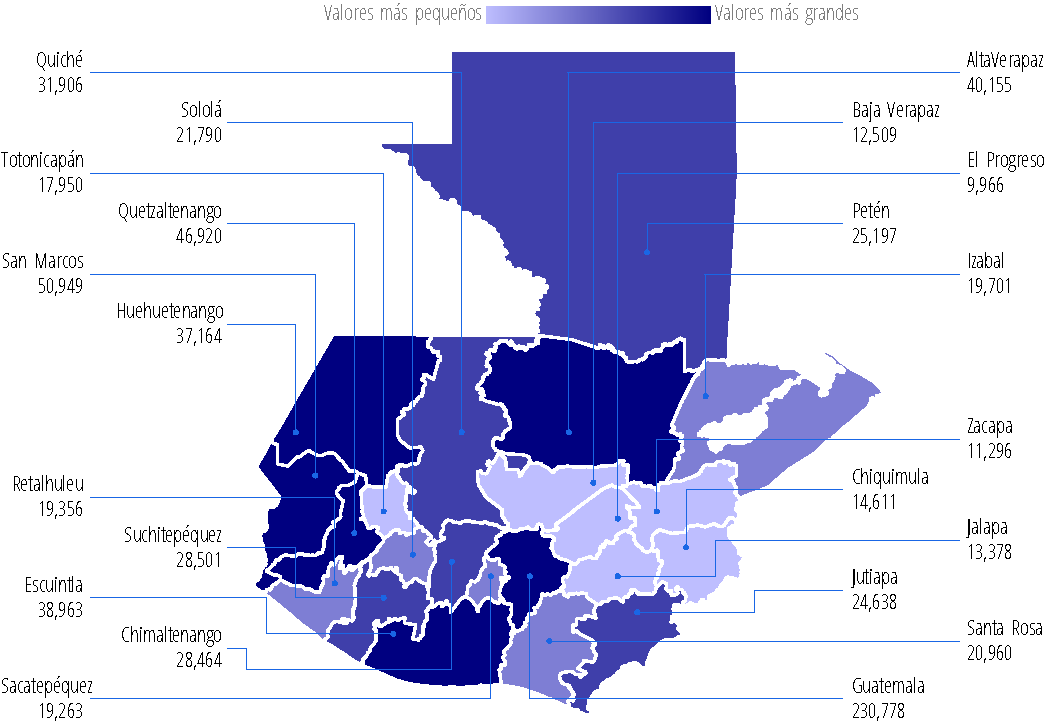
\includegraphics[width=52\cuadri]{graficas/basicos/1_7.pdf} }{Instituto Nacional de Estadística, con datos del Ministerio de Educación}




\INEchaptercarta[Indicadores de educación básica]{Indicadores\\ de educación básica}{}


\cajita{Cobertura bruta}{La tasa bruta de cobertura en básico establece una relación entre la inscripción inicial total sin distinción de edad, y la población de 13 a 15 años. 
	
	En el año 2009 fue de 66.7\% en el año 2014 fue de 68.4\%, presentando un aumento en 1.8 puntos porcentuales.}{Tasa bruta de cobertura del ciclo de educación básica}{República de Guatemala, serie histórica, en porcentaje}{\ \\[0mm]\begin{tikzpicture}[x=1pt,y=1pt]  % Created by tikzDevice version 0.10.1 on 2016-02-29 12:51:01
% !TEX encoding = UTF-8 Unicode
\definecolor{fillColor}{RGB}{255,255,255}
\path[use as bounding box,fill=fillColor,fill opacity=0.00] (0,0) rectangle (289.08,198.74);
\begin{scope}
\path[clip] (  0.00,  0.00) rectangle (289.08,198.74);

\path[] (  0.00,  0.00) rectangle (289.08,198.74);
\end{scope}
\begin{scope}
\path[clip] (  0.00,  0.00) rectangle (289.08,198.74);

\path[] ( -0.52, 15.61) rectangle (280.54,191.48);

\path[] (  0.00, 48.75) --
	(280.54, 48.75);

\path[] (  0.00, 99.02) --
	(280.54, 99.02);

\path[] (  0.00,149.30) --
	(280.54,149.30);

\path[] (  0.00, 23.61) --
	(280.54, 23.61);

\path[] (  0.00, 73.88) --
	(280.54, 73.88);

\path[] (  0.00,124.16) --
	(280.54,124.16);

\path[] (  0.00,174.44) --
	(280.54,174.44);

\path[] ( 26.68, 15.61) --
	( 26.68,191.48);

\path[] ( 72.01, 15.61) --
	( 72.01,191.48);

\path[] (117.35, 15.61) --
	(117.35,191.48);

\path[] (162.68, 15.61) --
	(162.68,191.48);

\path[] (208.01, 15.61) --
	(208.01,191.48);

\path[] (253.34, 15.61) --
	(253.34,191.48);
\definecolor{drawColor}{RGB}{0,0,255}

\path[draw=drawColor,line width= 1.7pt,line join=round] ( 26.68,140.75) --
	( 72.01,183.49) --
	(117.35,177.25) --
	(162.68,166.90) --
	(208.01,167.70) --
	(253.34,158.65);
\definecolor{drawColor}{RGB}{0,0,0}

\node[text=drawColor,anchor=base,inner sep=0pt, outer sep=0pt, scale=  1.02] at ( 26.68,128.84) {66.7};

\node[text=drawColor,anchor=base,inner sep=0pt, outer sep=0pt, scale=  1.02] at ( 72.01,187.46) {70.9};

\node[text=drawColor,anchor=base west,inner sep=0pt, outer sep=0pt, scale=  1.02] at (117.35,181.23) {70.3};

\node[text=drawColor,anchor=base,inner sep=0pt, outer sep=0pt, scale=  1.02] at (162.68,154.98) {69.2};

\node[text=drawColor,anchor=base,inner sep=0pt, outer sep=0pt, scale=  1.02] at (208.01,171.67) {69.3};

\node[text=drawColor,anchor=base,inner sep=0pt, outer sep=0pt, scale=  1.02] at (253.34,146.74) {68.4};

\path[draw=drawColor,line width= 0.1pt,line join=round] (  0.00, 23.61) -- (280.54, 23.61);

\path[] ( -0.52, 15.61) rectangle (280.54,191.48);
\end{scope}
\begin{scope}
\path[clip] (  0.00,  0.00) rectangle (289.08,198.74);

\path[] (  0.00, 15.61) --
	(280.54, 15.61);
\end{scope}
\begin{scope}
\path[clip] (  0.00,  0.00) rectangle (289.08,198.74);

\path[] ( 26.68, 12.86) --
	( 26.68, 15.61);

\path[] ( 72.01, 12.86) --
	( 72.01, 15.61);

\path[] (117.35, 12.86) --
	(117.35, 15.61);

\path[] (162.68, 12.86) --
	(162.68, 15.61);

\path[] (208.01, 12.86) --
	(208.01, 15.61);

\path[] (253.34, 12.86) --
	(253.34, 15.61);
\end{scope}
\begin{scope}
\path[clip] (  0.00,  0.00) rectangle (289.08,198.74);
\definecolor{drawColor}{RGB}{0,0,0}

\node[text=drawColor,anchor=base,inner sep=0pt, outer sep=0pt, scale=  1.00] at ( 26.68,  2.85) {2009};

\node[text=drawColor,anchor=base,inner sep=0pt, outer sep=0pt, scale=  1.00] at ( 72.01,  2.85) {2010};

\node[text=drawColor,anchor=base,inner sep=0pt, outer sep=0pt, scale=  1.00] at (117.35,  2.85) {2011};

\node[text=drawColor,anchor=base,inner sep=0pt, outer sep=0pt, scale=  1.00] at (162.68,  2.85) {2012};

\node[text=drawColor,anchor=base,inner sep=0pt, outer sep=0pt, scale=  1.00] at (208.01,  2.85) {2013};

\node[text=drawColor,anchor=base,inner sep=0pt, outer sep=0pt, scale=  1.00] at (253.34,  2.85) {2014};
\end{scope}
  \end{tikzpicture}}{Instituto Nacional de Estadística, con datos del Ministerio de Educación}

\cajita{Cobertura bruta por sexo}{La tasa bruta de cobertura en básico por sexo fue de 72.3\% para hombres y 64.5\% para mujeres.}{Tasa bruta de cobertura del ciclo de educación básica, por sexo}{República de Guatemala, año 2014, en porcentaje}{\ \\[0mm]\begin{tikzpicture}[x=1pt,y=1pt]  % Created by tikzDevice version 0.10.1 on 2016-02-29 12:51:21
% !TEX encoding = UTF-8 Unicode
\definecolor{fillColor}{RGB}{255,255,255}
\path[use as bounding box,fill=fillColor,fill opacity=0.00] (0,0) rectangle (289.08,198.74);
\begin{scope}
\path[clip] (  0.00,  0.00) rectangle (289.08,198.74);

\path[] (  0.00,  0.00) rectangle (289.08,198.74);
\end{scope}
\begin{scope}
\path[clip] (  0.00,  0.00) rectangle (289.08,198.74);

\path[] (  0.00, 12.77) rectangle (289.08,181.67);

\path[] ( 54.20, 12.77) --
	( 54.20,181.67);

\path[] (144.54, 12.77) --
	(144.54,181.67);

\path[] (234.88, 12.77) --
	(234.88,181.67);
\definecolor{drawColor}{RGB}{0,0,255}
\definecolor{fillColor}{RGB}{0,0,255}

\path[draw=drawColor,line width= 0.6pt,line join=round,fill=fillColor] ( 36.13, 20.44) rectangle ( 72.27,165.79);

\path[draw=drawColor,line width= 0.6pt,line join=round,fill=fillColor] (126.47, 20.44) rectangle (162.61,173.99);

\path[draw=drawColor,line width= 0.6pt,line join=round,fill=fillColor] (216.81, 20.44) rectangle (252.95,157.40);
\definecolor{drawColor}{RGB}{0,0,0}

\path[draw=drawColor,line width= 0.1pt,line join=round] (  0.00, 20.44) -- (289.08, 20.44);

\node[text=drawColor,anchor=base,inner sep=0pt, outer sep=0pt, scale=  1.02] at ( 54.20,169.77) {68.4};

\node[text=drawColor,anchor=base,inner sep=0pt, outer sep=0pt, scale=  1.02] at (144.54,177.96) {72.3};

\node[text=drawColor,anchor=base,inner sep=0pt, outer sep=0pt, scale=  1.02] at (234.88,161.38) {64.5};

\path[] (  0.00, 12.77) rectangle (289.08,181.67);
\end{scope}
\begin{scope}
\path[clip] (  0.00,  0.00) rectangle (289.08,198.74);

\path[] (  0.00, 12.77) --
	(289.08, 12.77);
\end{scope}
\begin{scope}
\path[clip] (  0.00,  0.00) rectangle (289.08,198.74);

\path[] ( 54.20, 10.02) --
	( 54.20, 12.77);

\path[] (144.54, 10.02) --
	(144.54, 12.77);

\path[] (234.88, 10.02) --
	(234.88, 12.77);
\end{scope}
\begin{scope}
\path[clip] (  0.00,  0.00) rectangle (289.08,198.74);
\definecolor{drawColor}{RGB}{0,0,0}

\node[text=drawColor,anchor=base,inner sep=0pt, outer sep=0pt, scale=  1.00] at ( 54.20, -0.00) {Total};

\node[text=drawColor,anchor=base,inner sep=0pt, outer sep=0pt, scale=  1.00] at (144.54, -0.00) {Hombre};

\node[text=drawColor,anchor=base,inner sep=0pt, outer sep=0pt, scale=  1.00] at (234.88, -0.00) {Mujer};
\end{scope}
  \end{tikzpicture}}{Instituto Nacional de Estadística, con datos del Ministerio de Educación}

\cajota{Cobertura bruta en los departamentos}{Los departamentos con las menores tasas brutas de cobertura en básico en el 2014 fueron: Alta Verapaz 44.0\%, Huehuetenango  39.9\% y Quiché 39.4\%.
	
	Los departamentos con las más altas tasas brutas de cobertura en básico:  Guatemala 110.4\%, El Progreso 88.7\% y Sacatepequez 86.1\%.}{Tasa bruta de cobertura del ciclo de educación básica}{Por departamento, año 2014, en porcentaje}{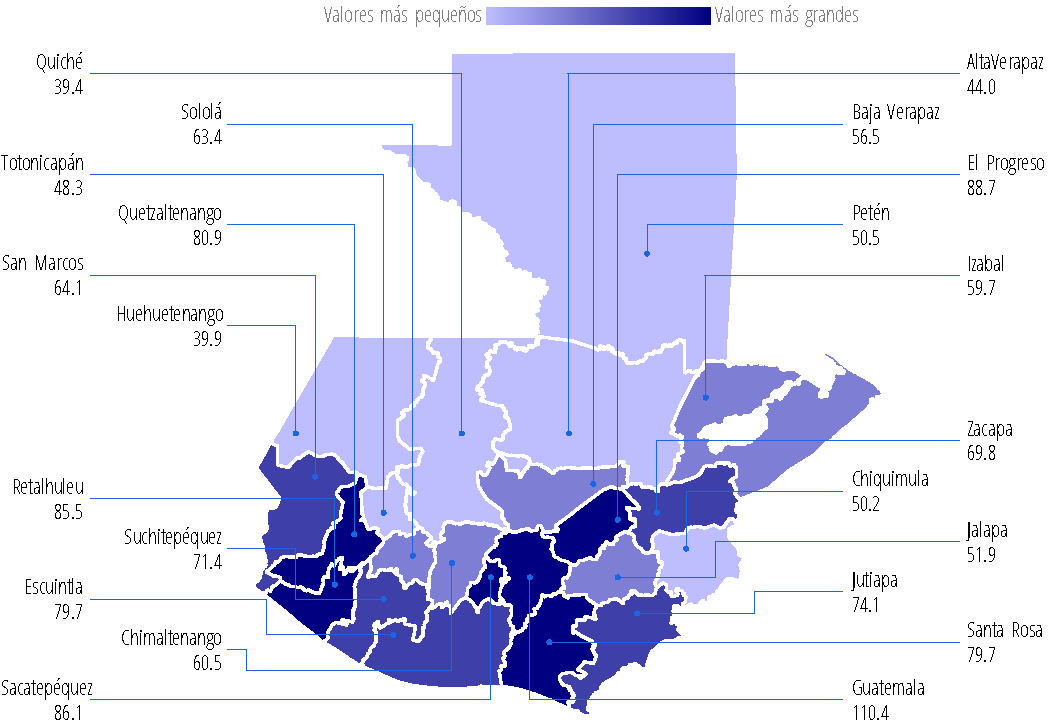
\includegraphics[width=52\cuadri]{graficas/basicos/1_10.pdf}}{Instituto Nacional de Estadística, con datos del Ministerio de Educación}

\cajita{Cobertura neta}{La tasa neta de cobertura en básico es la relación que existe entre la parte de la inscripción inicial que se encuentra en la edad escolar de 13 a 15 años y la población de esa misma edad.
	
	 En el año 2009 fue del 40.3\% y en el 2014 fue de 44.9\%, presentando un crecimiento de 4.7 puntos porcentuales.}{Tasa neta de cobertura del ciclo de educación básica}{República de Guatemala, serie histórica, en porcentaje}{\ \\[0mm]\begin{tikzpicture}[x=1pt,y=1pt]  % Created by tikzDevice version 0.7.0 on 2015-08-31 18:25:50
% !TEX encoding = UTF-8 Unicode
\definecolor[named]{fillColor}{rgb}{1.00,1.00,1.00}
\path[use as bounding box,fill=fillColor,fill opacity=0.00] (0,0) rectangle (289.08,198.74);
\begin{scope}
\path[clip] (  0.00,  0.00) rectangle (289.08,198.74);
\definecolor[named]{drawColor}{rgb}{1.00,1.00,1.00}

\path[draw=drawColor,line width= 0.6pt,line join=round,line cap=round] (  0.00,  0.00) rectangle (289.08,198.74);
\end{scope}
\begin{scope}
\path[clip] (  0.00,  0.00) rectangle (289.08,198.74);

\path[] (  1.64, 17.78) rectangle (280.54,191.48);

\path[] (  1.64, 53.87) --
	(280.54, 53.87);

\path[] (  1.64,110.27) --
	(280.54,110.27);

\path[] (  1.64,166.67) --
	(280.54,166.67);

\path[] (  1.64, 25.67) --
	(280.54, 25.67);

\path[] (  1.64, 82.07) --
	(280.54, 82.07);

\path[] (  1.64,138.47) --
	(280.54,138.47);

\path[] ( 33.83, 17.78) --
	( 33.83,191.48);

\path[] ( 87.46, 17.78) --
	( 87.46,191.48);

\path[] (141.09, 17.78) --
	(141.09,191.48);

\path[] (194.73, 17.78) --
	(194.73,191.48);

\path[] (248.36, 17.78) --
	(248.36,191.48);
\definecolor[named]{drawColor}{rgb}{0.00,0.00,1.00}

\path[draw=drawColor,line width= 1.7pt,line join=round] ( 33.83,141.85) --
	( 87.46,171.18) --
	(141.09,176.82) --
	(194.73,174.56) --
	(248.36,183.59);
\definecolor[named]{drawColor}{rgb}{0.00,0.00,0.00}

\node[text=drawColor,anchor=base,inner sep=0pt, outer sep=0pt, scale=  1.01] at ( 33.83,129.98) {40.3};

\node[text=drawColor,anchor=base east,inner sep=0pt, outer sep=0pt, scale=  1.01] at ( 84.34,171.18) {42.9};

\node[text=drawColor,anchor=base,inner sep=0pt, outer sep=0pt, scale=  1.01] at (141.09,180.78) {43.4};

\node[text=drawColor,anchor=base,inner sep=0pt, outer sep=0pt, scale=  1.01] at (194.73,162.69) {43.2};

\node[text=drawColor,anchor=base,inner sep=0pt, outer sep=0pt, scale=  1.01] at (248.36,187.54) {44.0};
\definecolor[named]{fillColor}{rgb}{0.00,0.00,0.00}

\path[draw=drawColor,line width= 0.1pt,line join=round,fill=fillColor] (  1.64, 25.67) -- (280.54, 25.67);
\end{scope}
\begin{scope}
\path[clip] (  0.00,  0.00) rectangle (289.08,198.74);

\path[] (  1.64, 17.78) --
	(  1.64,191.48);
\end{scope}
\begin{scope}
\path[clip] (  0.00,  0.00) rectangle (289.08,198.74);

\path[] (  0.00, 25.67) --
	(  1.64, 25.67);

\path[] (  0.00, 82.07) --
	(  1.64, 82.07);

\path[] (  0.00,138.47) --
	(  1.64,138.47);
\end{scope}
\begin{scope}
\path[clip] (  0.00,  0.00) rectangle (289.08,198.74);

\path[] (  1.64, 17.78) --
	(280.54, 17.78);
\end{scope}
\begin{scope}
\path[clip] (  0.00,  0.00) rectangle (289.08,198.74);

\path[] ( 33.83, 13.51) --
	( 33.83, 17.78);

\path[] ( 87.46, 13.51) --
	( 87.46, 17.78);

\path[] (141.09, 13.51) --
	(141.09, 17.78);

\path[] (194.73, 13.51) --
	(194.73, 17.78);

\path[] (248.36, 13.51) --
	(248.36, 17.78);
\end{scope}
\begin{scope}
\path[clip] (  0.00,  0.00) rectangle (289.08,198.74);
\definecolor[named]{drawColor}{rgb}{0.00,0.00,0.00}

\node[text=drawColor,anchor=base,inner sep=0pt, outer sep=0pt, scale=  1.00] at ( 33.83,  2.85) {2009};

\node[text=drawColor,anchor=base,inner sep=0pt, outer sep=0pt, scale=  1.00] at ( 87.46,  2.85) {2010};

\node[text=drawColor,anchor=base,inner sep=0pt, outer sep=0pt, scale=  1.00] at (141.09,  2.85) {2011};

\node[text=drawColor,anchor=base,inner sep=0pt, outer sep=0pt, scale=  1.00] at (194.73,  2.85) {2012};

\node[text=drawColor,anchor=base,inner sep=0pt, outer sep=0pt, scale=  1.00] at (248.36,  2.85) {2014};
\end{scope}
  \end{tikzpicture}}{Instituto Nacional de Estadística, con datos del Ministerio de Educación}

\cajita{Cobertura neta por sexo}{La tasa neta de cobertura en básico por sexo fue de 46.1\% para hombres y 43.8\% para las mujeres.}{Tasa neta de cobertura del ciclo de educación básica, por sexo}{República de Guatemala, año 2014, en porcentaje}{\ \\[0mm]\begin{tikzpicture}[x=1pt,y=1pt]  % Created by tikzDevice version 0.10.1 on 2016-02-29 12:51:44
% !TEX encoding = UTF-8 Unicode
\definecolor{fillColor}{RGB}{255,255,255}
\path[use as bounding box,fill=fillColor,fill opacity=0.00] (0,0) rectangle (289.08,198.74);
\begin{scope}
\path[clip] (  0.00,  0.00) rectangle (289.08,198.74);

\path[] (  0.00,  0.00) rectangle (289.08,198.74);
\end{scope}
\begin{scope}
\path[clip] (  0.00,  0.00) rectangle (289.08,198.74);

\path[] (  0.00, 12.77) rectangle (289.08,181.67);

\path[] ( 54.20, 12.77) --
	( 54.20,181.67);

\path[] (144.54, 12.77) --
	(144.54,181.67);

\path[] (234.88, 12.77) --
	(234.88,181.67);
\definecolor{drawColor}{RGB}{0,0,255}
\definecolor{fillColor}{RGB}{0,0,255}

\path[draw=drawColor,line width= 0.6pt,line join=round,fill=fillColor] ( 36.13, 20.44) rectangle ( 72.27,170.26);

\path[draw=drawColor,line width= 0.6pt,line join=round,fill=fillColor] (126.47, 20.44) rectangle (162.61,173.99);

\path[draw=drawColor,line width= 0.6pt,line join=round,fill=fillColor] (216.81, 20.44) rectangle (252.95,166.46);
\definecolor{drawColor}{RGB}{0,0,0}

\path[draw=drawColor,line width= 0.1pt,line join=round] (  0.00, 20.44) -- (289.08, 20.44);

\node[text=drawColor,anchor=base,inner sep=0pt, outer sep=0pt, scale=  1.02] at ( 54.20,174.23) {44.9};

\node[text=drawColor,anchor=base,inner sep=0pt, outer sep=0pt, scale=  1.02] at (144.54,177.96) {46.1};

\node[text=drawColor,anchor=base,inner sep=0pt, outer sep=0pt, scale=  1.02] at (234.88,170.43) {43.8};

\path[] (  0.00, 12.77) rectangle (289.08,181.67);
\end{scope}
\begin{scope}
\path[clip] (  0.00,  0.00) rectangle (289.08,198.74);

\path[] (  0.00, 12.77) --
	(289.08, 12.77);
\end{scope}
\begin{scope}
\path[clip] (  0.00,  0.00) rectangle (289.08,198.74);

\path[] ( 54.20, 10.02) --
	( 54.20, 12.77);

\path[] (144.54, 10.02) --
	(144.54, 12.77);

\path[] (234.88, 10.02) --
	(234.88, 12.77);
\end{scope}
\begin{scope}
\path[clip] (  0.00,  0.00) rectangle (289.08,198.74);
\definecolor{drawColor}{RGB}{0,0,0}

\node[text=drawColor,anchor=base,inner sep=0pt, outer sep=0pt, scale=  1.00] at ( 54.20, -0.00) {Total};

\node[text=drawColor,anchor=base,inner sep=0pt, outer sep=0pt, scale=  1.00] at (144.54, -0.00) {Hombre};

\node[text=drawColor,anchor=base,inner sep=0pt, outer sep=0pt, scale=  1.00] at (234.88, -0.00) {Mujer};
\end{scope}
  \end{tikzpicture}}{Instituto Nacional de Estadística, con datos del Ministerio de Educación}

\cajota{Cobertura neta en los departamentos}{Los departamentos con las menores tasas  netas de cobertura en básico en el 2014 fueron: Huehuetenango 26.1\%, Quiché 24.7\% y Alta Verapaz 24.4\%.
	
	 Los departamentos con las mayores tasas netas de cobertura en básico fueron: Guatemala 72.5\%, El Progreso 60.5\% y Sacatepéquez 58.4\%.}{Tasa neta de cobertura del ciclo de educación básica}{Por departamento, año 2014, en porcentaje}{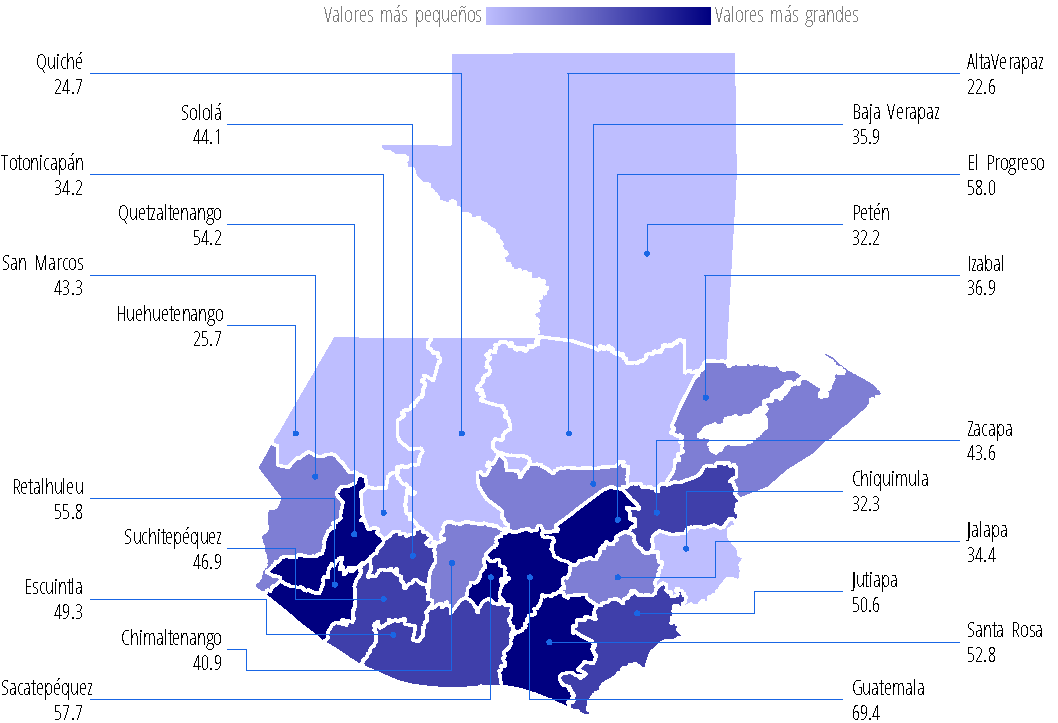
\includegraphics[width=52\cuadri]{graficas/basicos/1_13.pdf}}{Instituto Nacional de Estadística, con datos del Ministerio de Educación}




\cajita{Repitencia}{La tasa de repitencia en básico es la relación que existe entre el número de repitentes y el número de alumnos que en el año  estaban inscritos en el mismo grado.
	
	En el año 2009 el 3.1\% y en el año 2014 fue de 4.0\%, presentando un crecimiento de 0.9 puntos porcentuales.}{Tasa de repitencia del ciclo de educación básica}{República de Guatemala, serie histórica, en porcentaje}{\ \\[0mm]\begin{tikzpicture}[x=1pt,y=1pt]  % Created by tikzDevice version 0.7.0 on 2015-08-31 18:26:28
% !TEX encoding = UTF-8 Unicode
\definecolor[named]{fillColor}{rgb}{1.00,1.00,1.00}
\path[use as bounding box,fill=fillColor,fill opacity=0.00] (0,0) rectangle (289.08,198.74);
\begin{scope}
\path[clip] (  0.00,  0.00) rectangle (289.08,198.74);
\definecolor[named]{drawColor}{rgb}{1.00,1.00,1.00}

\path[draw=drawColor,line width= 0.6pt,line join=round,line cap=round] (  0.00,  0.00) rectangle (289.08,198.74);
\end{scope}
\begin{scope}
\path[clip] (  0.00,  0.00) rectangle (289.08,198.74);

\path[] ( -2.73, 17.78) rectangle (280.54,191.48);

\path[] (  0.00, 53.87) --
	(280.54, 53.87);

\path[] (  0.00,110.27) --
	(280.54,110.27);

\path[] (  0.00,166.67) --
	(280.54,166.67);

\path[] (  0.00, 25.67) --
	(280.54, 25.67);

\path[] (  0.00, 82.07) --
	(280.54, 82.07);

\path[] (  0.00,138.47) --
	(280.54,138.47);

\path[] ( 29.95, 17.78) --
	( 29.95,191.48);

\path[] ( 84.43, 17.78) --
	( 84.43,191.48);

\path[] (138.90, 17.78) --
	(138.90,191.48);

\path[] (193.38, 17.78) --
	(193.38,191.48);

\path[] (247.86, 17.78) --
	(247.86,191.48);
\definecolor[named]{drawColor}{rgb}{0.00,0.00,1.00}

\path[draw=drawColor,line width= 1.7pt,line join=round] ( 29.95,113.09) --
	( 84.43,110.27) --
	(138.90,104.63) --
	(193.38,183.59) --
	(247.86,152.57);
\definecolor[named]{drawColor}{rgb}{0.00,0.00,0.00}

\node[text=drawColor,anchor=base,inner sep=0pt, outer sep=0pt, scale=  1.01] at ( 29.95,117.05) {3.1};

\node[text=drawColor,anchor=base west,inner sep=0pt, outer sep=0pt, scale=  1.01] at ( 84.43,114.23) {3.0};

\node[text=drawColor,anchor=base,inner sep=0pt, outer sep=0pt, scale=  1.01] at (138.90, 92.76) {2.8};

\node[text=drawColor,anchor=base,inner sep=0pt, outer sep=0pt, scale=  1.01] at (193.38,187.54) {5.6};

\node[text=drawColor,anchor=base,inner sep=0pt, outer sep=0pt, scale=  1.01] at (247.86,140.70) {4.5};
\definecolor[named]{fillColor}{rgb}{0.00,0.00,0.00}

\path[draw=drawColor,line width= 0.1pt,line join=round,fill=fillColor] (  0.00, 25.67) -- (280.54, 25.67);
\end{scope}
\begin{scope}
\path[clip] (  0.00,  0.00) rectangle (289.08,198.74);

\path[] (  0.00, 17.78) --
	(280.54, 17.78);
\end{scope}
\begin{scope}
\path[clip] (  0.00,  0.00) rectangle (289.08,198.74);

\path[] ( 29.95, 13.51) --
	( 29.95, 17.78);

\path[] ( 84.43, 13.51) --
	( 84.43, 17.78);

\path[] (138.90, 13.51) --
	(138.90, 17.78);

\path[] (193.38, 13.51) --
	(193.38, 17.78);

\path[] (247.86, 13.51) --
	(247.86, 17.78);
\end{scope}
\begin{scope}
\path[clip] (  0.00,  0.00) rectangle (289.08,198.74);
\definecolor[named]{drawColor}{rgb}{0.00,0.00,0.00}

\node[text=drawColor,anchor=base,inner sep=0pt, outer sep=0pt, scale=  1.00] at ( 29.95,  2.85) {2009};

\node[text=drawColor,anchor=base,inner sep=0pt, outer sep=0pt, scale=  1.00] at ( 84.43,  2.85) {2010};

\node[text=drawColor,anchor=base,inner sep=0pt, outer sep=0pt, scale=  1.00] at (138.90,  2.85) {2011};

\node[text=drawColor,anchor=base,inner sep=0pt, outer sep=0pt, scale=  1.00] at (193.38,  2.85) {2012};

\node[text=drawColor,anchor=base,inner sep=0pt, outer sep=0pt, scale=  1.00] at (247.86,  2.85) {2014};
\end{scope}
  \end{tikzpicture}}{Instituto Nacional de Estadística, con datos del Ministerio de Educación}

\cajita{Repitencia por sexo}{La tasa de repitencia en básico por sexo fue del 4.3\% para hombres y 3.7\% para las mujeres.}{Tasa de repitencia del ciclo de educación básica, por sexo}{República de Guatemala, año 2014, en porcentaje}{\ \\[0mm]\begin{tikzpicture}[x=1pt,y=1pt]  % Created by tikzDevice version 0.10.1 on 2016-02-29 12:52:09
% !TEX encoding = UTF-8 Unicode
\definecolor{fillColor}{RGB}{255,255,255}
\path[use as bounding box,fill=fillColor,fill opacity=0.00] (0,0) rectangle (289.08,198.74);
\begin{scope}
\path[clip] (  0.00,  0.00) rectangle (289.08,198.74);

\path[] (  0.00,  0.00) rectangle (289.08,198.74);
\end{scope}
\begin{scope}
\path[clip] (  0.00,  0.00) rectangle (289.08,198.74);

\path[] (  0.00, 12.77) rectangle (289.08,181.67);

\path[] ( 54.20, 12.77) --
	( 54.20,181.67);

\path[] (144.54, 12.77) --
	(144.54,181.67);

\path[] (234.88, 12.77) --
	(234.88,181.67);
\definecolor{drawColor}{RGB}{0,0,255}
\definecolor{fillColor}{RGB}{0,0,255}

\path[draw=drawColor,line width= 0.6pt,line join=round,fill=fillColor] ( 36.13, 20.44) rectangle ( 72.27,163.38);

\path[draw=drawColor,line width= 0.6pt,line join=round,fill=fillColor] (126.47, 20.44) rectangle (162.61,173.99);

\path[draw=drawColor,line width= 0.6pt,line join=round,fill=fillColor] (216.81, 20.44) rectangle (252.95,151.35);
\definecolor{drawColor}{RGB}{0,0,0}

\path[draw=drawColor,line width= 0.1pt,line join=round] (  0.00, 20.44) -- (289.08, 20.44);

\node[text=drawColor,anchor=base,inner sep=0pt, outer sep=0pt, scale=  1.02] at ( 54.20,167.35) {4.0};

\node[text=drawColor,anchor=base,inner sep=0pt, outer sep=0pt, scale=  1.02] at (144.54,177.96) {4.3};

\node[text=drawColor,anchor=base,inner sep=0pt, outer sep=0pt, scale=  1.02] at (234.88,155.32) {3.7};

\path[] (  0.00, 12.77) rectangle (289.08,181.67);
\end{scope}
\begin{scope}
\path[clip] (  0.00,  0.00) rectangle (289.08,198.74);

\path[] (  0.00, 12.77) --
	(289.08, 12.77);
\end{scope}
\begin{scope}
\path[clip] (  0.00,  0.00) rectangle (289.08,198.74);

\path[] ( 54.20, 10.02) --
	( 54.20, 12.77);

\path[] (144.54, 10.02) --
	(144.54, 12.77);

\path[] (234.88, 10.02) --
	(234.88, 12.77);
\end{scope}
\begin{scope}
\path[clip] (  0.00,  0.00) rectangle (289.08,198.74);
\definecolor{drawColor}{RGB}{0,0,0}

\node[text=drawColor,anchor=base,inner sep=0pt, outer sep=0pt, scale=  1.00] at ( 54.20, -0.00) {Total};

\node[text=drawColor,anchor=base,inner sep=0pt, outer sep=0pt, scale=  1.00] at (144.54, -0.00) {Hombre};

\node[text=drawColor,anchor=base,inner sep=0pt, outer sep=0pt, scale=  1.00] at (234.88, -0.00) {Mujer};
\end{scope}
  \end{tikzpicture}}{Instituto Nacional de Estadística, con datos del Ministerio de Educación}

\cajota{Repitencia en los departamentos}{Los departamentos con las menores tasas de repitencia en básico en el 2013 fueron: Retalhuleu 2.2\%, Petén 2.0\% y Jutiapa 1.7\%.
	
	 Los departamentos con las mayores tasas de repitencia en básico fueron: Sacatepéquez 8.0\%, Sololá 6.8\% y Totonicapán 5.7\%. El departamento de Guatemala presentó una tasa de repitencia de 4.3\%.}{Tasa de repitencia del ciclo de educación básica}{Por departamento, año 2014, en porcentaje}{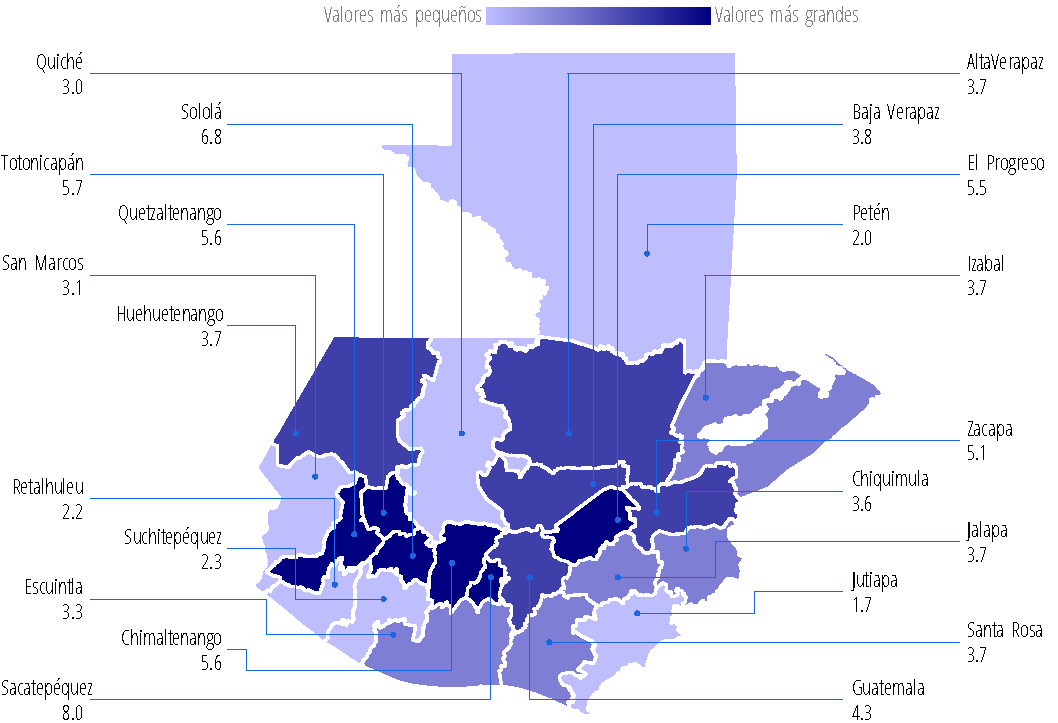
\includegraphics[width=52\cuadri]{graficas/basicos/1_16.pdf}}{Instituto Nacional de Estadística, con datos del Ministerio de Educación}






\cajita{Sobre-edad}{La tasa de sobre-edad en básico es la relación que existe entre la cantidad de alumnos inscritos en los diferentes grados de un nivel educativo, con dos o más años de atraso escolar por encima de la edad correspondiente al grado de estudio.
	
	En el año 2009 fue del 34\% y en el año 2014 fue de 23.6\%, el cual fue una disminución de  10.4 puntos porcentuales.}{Tasa de sobre-edad del ciclo de educación básica}{República de Guatemala, serie histórica, en porcentaje}{\ \\[0mm]\begin{tikzpicture}[x=1pt,y=1pt]  % Created by tikzDevice version 0.7.0 on 2015-08-31 18:27:35
% !TEX encoding = UTF-8 Unicode
\definecolor[named]{fillColor}{rgb}{1.00,1.00,1.00}
\path[use as bounding box,fill=fillColor,fill opacity=0.00] (0,0) rectangle (289.08,198.74);
\begin{scope}
\path[clip] (  0.00,  0.00) rectangle (289.08,198.74);
\definecolor[named]{drawColor}{rgb}{1.00,1.00,1.00}

\path[draw=drawColor,line width= 0.6pt,line join=round,line cap=round] (  0.00,  0.00) rectangle (289.08,198.74);
\end{scope}
\begin{scope}
\path[clip] (  0.00,  0.00) rectangle (289.08,198.74);

\path[] (  1.64, 17.78) rectangle (280.54,191.48);

\path[] (  1.64, 25.67) --
	(280.54, 25.67);

\path[] (  1.64, 59.70) --
	(280.54, 59.70);

\path[] (  1.64, 93.74) --
	(280.54, 93.74);

\path[] (  1.64,127.77) --
	(280.54,127.77);

\path[] (  1.64,161.81) --
	(280.54,161.81);

\path[] (  1.64, 42.69) --
	(280.54, 42.69);

\path[] (  1.64, 76.72) --
	(280.54, 76.72);

\path[] (  1.64,110.76) --
	(280.54,110.76);

\path[] (  1.64,144.79) --
	(280.54,144.79);

\path[] (  1.64,178.82) --
	(280.54,178.82);

\path[] ( 33.83, 17.78) --
	( 33.83,191.48);

\path[] ( 87.46, 17.78) --
	( 87.46,191.48);

\path[] (141.09, 17.78) --
	(141.09,191.48);

\path[] (194.73, 17.78) --
	(194.73,191.48);

\path[] (248.36, 17.78) --
	(248.36,191.48);
\definecolor[named]{drawColor}{rgb}{0.00,0.00,1.00}

\path[draw=drawColor,line width= 1.7pt,line join=round] ( 33.83,124.37) --
	( 87.46,183.59) --
	(141.09,110.41) --
	(194.73,105.99) --
	(248.36,104.63);
\definecolor[named]{drawColor}{rgb}{0.00,0.00,0.00}

\node[text=drawColor,anchor=base,inner sep=0pt, outer sep=0pt, scale=  1.01] at ( 33.83,112.50) {34.0};

\node[text=drawColor,anchor=base,inner sep=0pt, outer sep=0pt, scale=  1.01] at ( 87.46,187.54) {51.4};

\node[text=drawColor,anchor=base west,inner sep=0pt, outer sep=0pt, scale=  1.01] at (141.09,114.37) {29.9};

\node[text=drawColor,anchor=base west,inner sep=0pt, outer sep=0pt, scale=  1.01] at (194.73,109.95) {28.6};

\node[text=drawColor,anchor=base,inner sep=0pt, outer sep=0pt, scale=  1.01] at (248.36, 92.76) {28.2};
\definecolor[named]{fillColor}{rgb}{0.00,0.00,0.00}

\path[draw=drawColor,line width= 0.1pt,line join=round,fill=fillColor] (  1.64, 25.67) -- (280.54, 25.67);
\end{scope}
\begin{scope}
\path[clip] (  0.00,  0.00) rectangle (289.08,198.74);

\path[] (  1.64, 17.78) --
	(  1.64,191.48);
\end{scope}
\begin{scope}
\path[clip] (  0.00,  0.00) rectangle (289.08,198.74);

\path[] (  0.00, 42.69) --
	(  1.64, 42.69);

\path[] (  0.00, 76.72) --
	(  1.64, 76.72);

\path[] (  0.00,110.76) --
	(  1.64,110.76);

\path[] (  0.00,144.79) --
	(  1.64,144.79);

\path[] (  0.00,178.82) --
	(  1.64,178.82);
\end{scope}
\begin{scope}
\path[clip] (  0.00,  0.00) rectangle (289.08,198.74);

\path[] (  1.64, 17.78) --
	(280.54, 17.78);
\end{scope}
\begin{scope}
\path[clip] (  0.00,  0.00) rectangle (289.08,198.74);

\path[] ( 33.83, 13.51) --
	( 33.83, 17.78);

\path[] ( 87.46, 13.51) --
	( 87.46, 17.78);

\path[] (141.09, 13.51) --
	(141.09, 17.78);

\path[] (194.73, 13.51) --
	(194.73, 17.78);

\path[] (248.36, 13.51) --
	(248.36, 17.78);
\end{scope}
\begin{scope}
\path[clip] (  0.00,  0.00) rectangle (289.08,198.74);
\definecolor[named]{drawColor}{rgb}{0.00,0.00,0.00}

\node[text=drawColor,anchor=base,inner sep=0pt, outer sep=0pt, scale=  1.00] at ( 33.83,  2.85) {2009};

\node[text=drawColor,anchor=base,inner sep=0pt, outer sep=0pt, scale=  1.00] at ( 87.46,  2.85) {2010};

\node[text=drawColor,anchor=base,inner sep=0pt, outer sep=0pt, scale=  1.00] at (141.09,  2.85) {2011};

\node[text=drawColor,anchor=base,inner sep=0pt, outer sep=0pt, scale=  1.00] at (194.73,  2.85) {2012};

\node[text=drawColor,anchor=base,inner sep=0pt, outer sep=0pt, scale=  1.00] at (248.36,  2.85) {2014};
\end{scope}
  \end{tikzpicture}}{Instituto Nacional de Estadística, con datos del Ministerio de Educación}

\cajita{Sobre-edad por sexo}{La tasa de sobre-edad en básico por sexo en el 2014 fue de 26.5\% para hombres y 20.3\% para las mujeres.}{Tasa de sobre-edad del ciclo de educación básica, por sexo}{República de Guatemala, año 2014, en porcentaje}{\ \\[0mm]\begin{tikzpicture}[x=1pt,y=1pt]  % Created by tikzDevice version 0.10.1 on 2016-02-29 12:52:31
% !TEX encoding = UTF-8 Unicode
\definecolor{fillColor}{RGB}{255,255,255}
\path[use as bounding box,fill=fillColor,fill opacity=0.00] (0,0) rectangle (289.08,198.74);
\begin{scope}
\path[clip] (  0.00,  0.00) rectangle (289.08,198.74);

\path[] (  0.00,  0.00) rectangle (289.08,198.74);
\end{scope}
\begin{scope}
\path[clip] (  0.00,  0.00) rectangle (289.08,198.74);

\path[] (  0.00, 12.77) rectangle (289.08,181.67);

\path[] ( 54.20, 12.77) --
	( 54.20,181.67);

\path[] (144.54, 12.77) --
	(144.54,181.67);

\path[] (234.88, 12.77) --
	(234.88,181.67);
\definecolor{drawColor}{RGB}{0,0,255}
\definecolor{fillColor}{RGB}{0,0,255}

\path[draw=drawColor,line width= 0.6pt,line join=round,fill=fillColor] ( 36.13, 20.44) rectangle ( 72.27,157.20);

\path[draw=drawColor,line width= 0.6pt,line join=round,fill=fillColor] (126.47, 20.44) rectangle (162.61,173.99);

\path[draw=drawColor,line width= 0.6pt,line join=round,fill=fillColor] (216.81, 20.44) rectangle (252.95,137.97);
\definecolor{drawColor}{RGB}{0,0,0}

\path[draw=drawColor,line width= 0.1pt,line join=round] (  0.00, 20.44) -- (289.08, 20.44);

\node[text=drawColor,anchor=base,inner sep=0pt, outer sep=0pt, scale=  1.02] at ( 54.20,161.17) {23.6};

\node[text=drawColor,anchor=base,inner sep=0pt, outer sep=0pt, scale=  1.02] at (144.54,177.96) {26.5};

\node[text=drawColor,anchor=base,inner sep=0pt, outer sep=0pt, scale=  1.02] at (234.88,141.94) {20.3};

\path[] (  0.00, 12.77) rectangle (289.08,181.67);
\end{scope}
\begin{scope}
\path[clip] (  0.00,  0.00) rectangle (289.08,198.74);

\path[] (  0.00, 12.77) --
	(289.08, 12.77);
\end{scope}
\begin{scope}
\path[clip] (  0.00,  0.00) rectangle (289.08,198.74);

\path[] ( 54.20, 10.02) --
	( 54.20, 12.77);

\path[] (144.54, 10.02) --
	(144.54, 12.77);

\path[] (234.88, 10.02) --
	(234.88, 12.77);
\end{scope}
\begin{scope}
\path[clip] (  0.00,  0.00) rectangle (289.08,198.74);
\definecolor{drawColor}{RGB}{0,0,0}

\node[text=drawColor,anchor=base,inner sep=0pt, outer sep=0pt, scale=  1.00] at ( 54.20, -0.00) {Total};

\node[text=drawColor,anchor=base,inner sep=0pt, outer sep=0pt, scale=  1.00] at (144.54, -0.00) {Hombre};

\node[text=drawColor,anchor=base,inner sep=0pt, outer sep=0pt, scale=  1.00] at (234.88, -0.00) {Mujer};
\end{scope}
  \end{tikzpicture}}{Instituto Nacional de Estadística, con datos del Ministerio de Educación}

\cajota{Sobre-edad en los departamentos}{El mapa muestra en color celeste los departamentos con las menores tasas de sobre-edad en básico fueron: Totonicapán 19.0\%, Chimaltenango 17.8\% y Quetzaltenango 15.6\%.
	
	 Los departamentos con las mayores tasas  de sobre-edad en básico: Alta Verapaz 37.6\%, Petén 28.1\% y Quiché 27.5\%.
	 
	 El departamento de Guatemala tuvo un 24.8\%.}{Tasa de sobre-edad del ciclo de educación básica}{Por departamento, año 2014, en porcentaje}{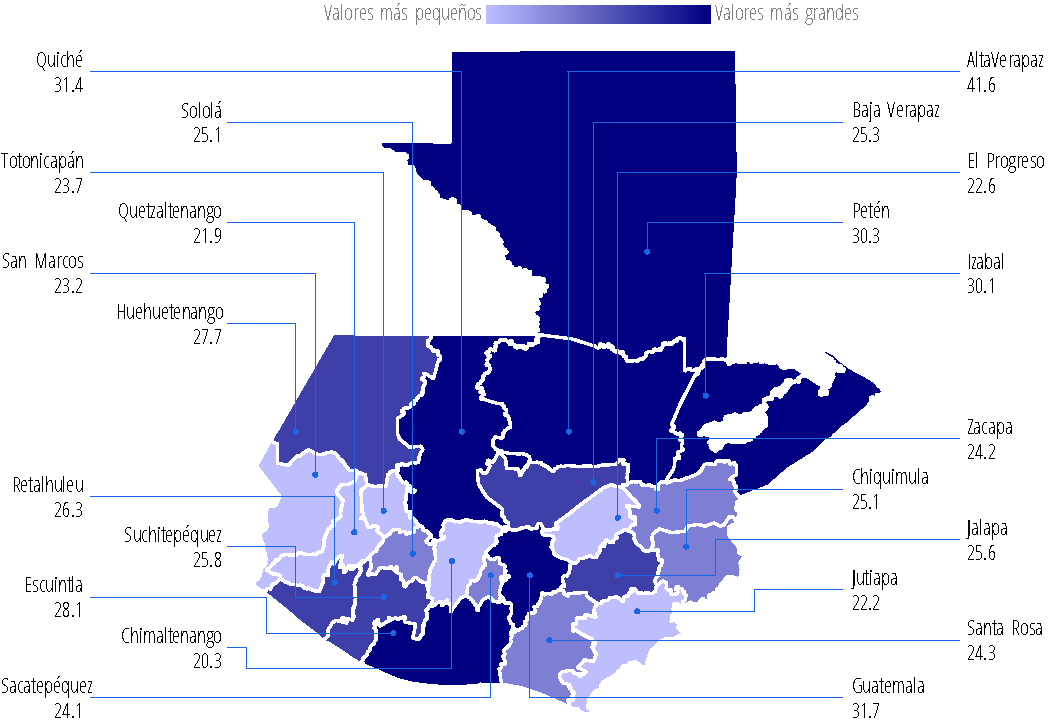
\includegraphics[width=52\cuadri]{graficas/basicos/1_19.pdf}}{Instituto Nacional de Estadística, con datos del Ministerio de Educación}





\cajita{Deserción}{La tasa de deserción en básico se refiere a la cantidad de alumnos que no concluyen el ciclo lectivo.
	
	En el año fue 2009 el 8.2\% y en el año 2014 fue de 4.1\%, que fue una disminución de 4.1 puntos porcentuales.}{Tasa de deserción del ciclo de educación básica}{República de Guatemala, serie histórica, en porcentaje}{\ \\[0mm]\begin{tikzpicture}[x=1pt,y=1pt]  % Created by tikzDevice version 0.7.0 on 2015-08-31 18:28:05
% !TEX encoding = UTF-8 Unicode
\definecolor[named]{fillColor}{rgb}{1.00,1.00,1.00}
\path[use as bounding box,fill=fillColor,fill opacity=0.00] (0,0) rectangle (289.08,198.74);
\begin{scope}
\path[clip] (  0.00,  0.00) rectangle (289.08,198.74);
\definecolor[named]{drawColor}{rgb}{1.00,1.00,1.00}

\path[draw=drawColor,line width= 0.6pt,line join=round,line cap=round] (  0.00,  0.00) rectangle (289.08,198.74);
\end{scope}
\begin{scope}
\path[clip] (  0.00,  0.00) rectangle (289.08,198.74);

\path[] (  8.28, 17.78) rectangle (280.54,191.48);

\path[] (  8.28, 44.84) --
	(280.54, 44.84);

\path[] (  8.28, 83.16) --
	(280.54, 83.16);

\path[] (  8.28,121.49) --
	(280.54,121.49);

\path[] (  8.28,159.82) --
	(280.54,159.82);

\path[] (  8.28, 25.67) --
	(280.54, 25.67);

\path[] (  8.28, 64.00) --
	(280.54, 64.00);

\path[] (  8.28,102.33) --
	(280.54,102.33);

\path[] (  8.28,140.66) --
	(280.54,140.66);

\path[] (  8.28,178.99) --
	(280.54,178.99);

\path[] ( 39.69, 17.78) --
	( 39.69,191.48);

\path[] ( 92.05, 17.78) --
	( 92.05,191.48);

\path[] (144.41, 17.78) --
	(144.41,191.48);

\path[] (196.77, 17.78) --
	(196.77,191.48);

\path[] (249.13, 17.78) --
	(249.13,191.48);
\definecolor[named]{drawColor}{rgb}{0.00,0.00,1.00}

\path[draw=drawColor,line width= 1.7pt,line join=round] ( 39.69,151.39) --
	( 92.05,183.59) --
	(144.41,105.40) --
	(196.77,131.46) --
	(249.13,116.13);
\definecolor[named]{drawColor}{rgb}{0.00,0.00,0.00}

\node[text=drawColor,anchor=base,inner sep=0pt, outer sep=0pt, scale=  1.01] at ( 39.69,139.52) {8.2};

\node[text=drawColor,anchor=base,inner sep=0pt, outer sep=0pt, scale=  1.01] at ( 92.05,187.54) {10.3};

\node[text=drawColor,anchor=base,inner sep=0pt, outer sep=0pt, scale=  1.01] at (144.41, 93.53) {5.2};

\node[text=drawColor,anchor=base,inner sep=0pt, outer sep=0pt, scale=  1.01] at (196.77,135.42) {6.9};

\node[text=drawColor,anchor=base,inner sep=0pt, outer sep=0pt, scale=  1.01] at (249.13,104.26) {5.9};
\definecolor[named]{fillColor}{rgb}{0.00,0.00,0.00}

\path[draw=drawColor,line width= 0.1pt,line join=round,fill=fillColor] (  8.28, 25.67) -- (280.54, 25.67);
\end{scope}
\begin{scope}
\path[clip] (  0.00,  0.00) rectangle (289.08,198.74);

\path[] (  8.28, 17.78) --
	(  8.28,191.48);
\end{scope}
\begin{scope}
\path[clip] (  0.00,  0.00) rectangle (289.08,198.74);
\definecolor[named]{drawColor}{rgb}{1.00,1.00,1.00}

\node[text=drawColor,text opacity=0.00,anchor=base east,inner sep=0pt, outer sep=0pt, scale=  1.00] at (  1.17, 21.76) {0.0};

\node[text=drawColor,text opacity=0.00,anchor=base east,inner sep=0pt, outer sep=0pt, scale=  1.00] at (  1.17, 60.09) {2.5};

\node[text=drawColor,text opacity=0.00,anchor=base east,inner sep=0pt, outer sep=0pt, scale=  1.00] at (  1.17, 98.42) {5.0};

\node[text=drawColor,text opacity=0.00,anchor=base east,inner sep=0pt, outer sep=0pt, scale=  1.00] at (  1.17,136.75) {7.5};

\node[text=drawColor,text opacity=0.00,anchor=base east,inner sep=0pt, outer sep=0pt, scale=  1.00] at (  1.17,175.08) {10.0};
\end{scope}
\begin{scope}
\path[clip] (  0.00,  0.00) rectangle (289.08,198.74);

\path[] (  4.01, 25.67) --
	(  8.28, 25.67);

\path[] (  4.01, 64.00) --
	(  8.28, 64.00);

\path[] (  4.01,102.33) --
	(  8.28,102.33);

\path[] (  4.01,140.66) --
	(  8.28,140.66);

\path[] (  4.01,178.99) --
	(  8.28,178.99);
\end{scope}
\begin{scope}
\path[clip] (  0.00,  0.00) rectangle (289.08,198.74);

\path[] (  8.28, 17.78) --
	(280.54, 17.78);
\end{scope}
\begin{scope}
\path[clip] (  0.00,  0.00) rectangle (289.08,198.74);

\path[] ( 39.69, 13.51) --
	( 39.69, 17.78);

\path[] ( 92.05, 13.51) --
	( 92.05, 17.78);

\path[] (144.41, 13.51) --
	(144.41, 17.78);

\path[] (196.77, 13.51) --
	(196.77, 17.78);

\path[] (249.13, 13.51) --
	(249.13, 17.78);
\end{scope}
\begin{scope}
\path[clip] (  0.00,  0.00) rectangle (289.08,198.74);
\definecolor[named]{drawColor}{rgb}{0.00,0.00,0.00}

\node[text=drawColor,anchor=base,inner sep=0pt, outer sep=0pt, scale=  1.00] at ( 39.69,  2.85) {2009};

\node[text=drawColor,anchor=base,inner sep=0pt, outer sep=0pt, scale=  1.00] at ( 92.05,  2.85) {2010};

\node[text=drawColor,anchor=base,inner sep=0pt, outer sep=0pt, scale=  1.00] at (144.41,  2.85) {2011};

\node[text=drawColor,anchor=base,inner sep=0pt, outer sep=0pt, scale=  1.00] at (196.77,  2.85) {2012};

\node[text=drawColor,anchor=base,inner sep=0pt, outer sep=0pt, scale=  1.00] at (249.13,  2.85) {2014};
\end{scope}
  \end{tikzpicture}}{Instituto Nacional de Estadística, con datos del Ministerio de Educación}

\cajita{Deserción por sexo}{La tasa de deserción en básico por sexo, representó el 5.2\% para hombres y 2.8\% para las mujeres.}{Tasa de deserción del ciclo de educación básica, por sexo}{República de Guatemala, año 2014, en porcentaje}{\ \\[0mm]\begin{tikzpicture}[x=1pt,y=1pt]  % Created by tikzDevice version 0.10.1 on 2016-02-29 12:52:59
% !TEX encoding = UTF-8 Unicode
\definecolor{fillColor}{RGB}{255,255,255}
\path[use as bounding box,fill=fillColor,fill opacity=0.00] (0,0) rectangle (289.08,198.74);
\begin{scope}
\path[clip] (  0.00,  0.00) rectangle (289.08,198.74);

\path[] (  0.00,  0.00) rectangle (289.08,198.74);
\end{scope}
\begin{scope}
\path[clip] (  0.00,  0.00) rectangle (289.08,198.74);

\path[] (  0.00, 12.77) rectangle (289.08,181.67);

\path[] ( 54.20, 12.77) --
	( 54.20,181.67);

\path[] (144.54, 12.77) --
	(144.54,181.67);

\path[] (234.88, 12.77) --
	(234.88,181.67);
\definecolor{drawColor}{RGB}{0,0,255}
\definecolor{fillColor}{RGB}{0,0,255}

\path[draw=drawColor,line width= 0.6pt,line join=round,fill=fillColor] ( 36.13, 20.44) rectangle ( 72.27,141.17);

\path[draw=drawColor,line width= 0.6pt,line join=round,fill=fillColor] (126.47, 20.44) rectangle (162.61,173.99);

\path[draw=drawColor,line width= 0.6pt,line join=round,fill=fillColor] (216.81, 20.44) rectangle (252.95,103.67);
\definecolor{drawColor}{RGB}{0,0,0}

\path[draw=drawColor,line width= 0.1pt,line join=round] (  0.00, 20.44) -- (289.08, 20.44);

\node[text=drawColor,anchor=base,inner sep=0pt, outer sep=0pt, scale=  1.02] at ( 54.20,145.14) {4.1};

\node[text=drawColor,anchor=base,inner sep=0pt, outer sep=0pt, scale=  1.02] at (144.54,177.96) {5.2};

\node[text=drawColor,anchor=base,inner sep=0pt, outer sep=0pt, scale=  1.02] at (234.88,107.64) {2.8};

\path[] (  0.00, 12.77) rectangle (289.08,181.67);
\end{scope}
\begin{scope}
\path[clip] (  0.00,  0.00) rectangle (289.08,198.74);

\path[] (  0.00, 12.77) --
	(289.08, 12.77);
\end{scope}
\begin{scope}
\path[clip] (  0.00,  0.00) rectangle (289.08,198.74);

\path[] ( 54.20, 10.02) --
	( 54.20, 12.77);

\path[] (144.54, 10.02) --
	(144.54, 12.77);

\path[] (234.88, 10.02) --
	(234.88, 12.77);
\end{scope}
\begin{scope}
\path[clip] (  0.00,  0.00) rectangle (289.08,198.74);
\definecolor{drawColor}{RGB}{0,0,0}

\node[text=drawColor,anchor=base,inner sep=0pt, outer sep=0pt, scale=  1.00] at ( 54.20, -0.00) {Total};

\node[text=drawColor,anchor=base,inner sep=0pt, outer sep=0pt, scale=  1.00] at (144.54, -0.00) {Hombre};

\node[text=drawColor,anchor=base,inner sep=0pt, outer sep=0pt, scale=  1.00] at (234.88, -0.00) {Mujer};
\end{scope}
  \end{tikzpicture}}{Instituto Nacional de Estadística, con datos del Ministerio de Educación}

\cajota{Deserción en los departamentos}{El mapa muestra en color celeste los departamentos con las menores tasas de deserción en básicos, que en el 2013 fueron: Izabal 2.9\%, Guatemala 2.6\% y Quetzaltenango 1.3\%.
	
	 Los departamentos con las mayores tasas  de deserción en básico: Huehuetenango 7.0\%, El Progreso 6.9\% y Sololá 6.3\%.}{Tasa de deserción del ciclo de educación básica}{Por departamento, año 2014, en porcentaje}{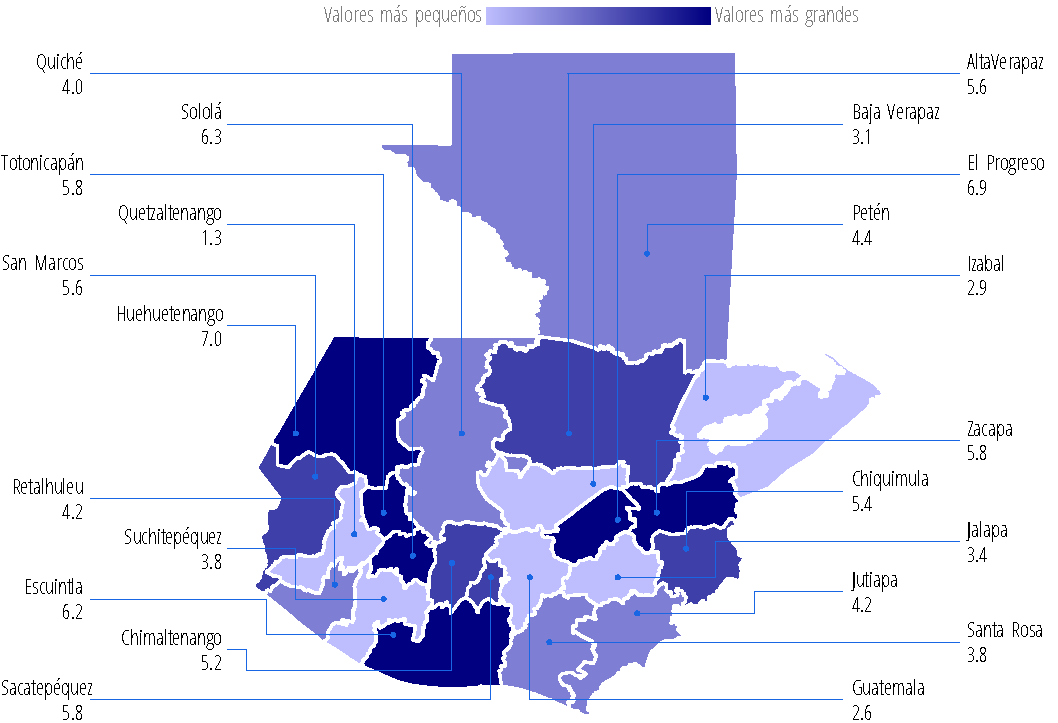
\includegraphics[width=52\cuadri]{graficas/basicos/1_22.pdf}}{Instituto Nacional de Estadística, con datos del Ministerio de Educación}




\cajita{Aprobación}{La tasa de aprobación en básico se refiere a la cantidad de alumnos que culminaron y aprobaron el ciclo lectivo.
	
	En el año 2009 fue del 68.4\% y en el año 2014 fue de 71.6\%, que representó un aumento en 3.2 puntos porcentuales.}{Tasa de aprobación del ciclo de educación básica}{República de Guatemala, serie histórica, en porcentaje}{\ \\[0mm]\begin{tikzpicture}[x=1pt,y=1pt]  % Created by tikzDevice version 0.10.1 on 2016-02-29 12:53:03
% !TEX encoding = UTF-8 Unicode
\definecolor{fillColor}{RGB}{255,255,255}
\path[use as bounding box,fill=fillColor,fill opacity=0.00] (0,0) rectangle (289.08,198.74);
\begin{scope}
\path[clip] (  0.00,  0.00) rectangle (289.08,198.74);

\path[] (  0.00,  0.00) rectangle (289.08,198.74);
\end{scope}
\begin{scope}
\path[clip] (  0.00,  0.00) rectangle (289.08,198.74);

\path[] ( -0.52, 15.61) rectangle (280.54,191.48);

\path[] (  0.00, 44.37) --
	(280.54, 44.37);

\path[] (  0.00, 85.90) --
	(280.54, 85.90);

\path[] (  0.00,127.43) --
	(280.54,127.43);

\path[] (  0.00,168.95) --
	(280.54,168.95);

\path[] (  0.00, 23.61) --
	(280.54, 23.61);

\path[] (  0.00, 65.13) --
	(280.54, 65.13);

\path[] (  0.00,106.66) --
	(280.54,106.66);

\path[] (  0.00,148.19) --
	(280.54,148.19);

\path[] (  0.00,189.72) --
	(280.54,189.72);

\path[] ( 26.68, 15.61) --
	( 26.68,191.48);

\path[] ( 72.01, 15.61) --
	( 72.01,191.48);

\path[] (117.35, 15.61) --
	(117.35,191.48);

\path[] (162.68, 15.61) --
	(162.68,191.48);

\path[] (208.01, 15.61) --
	(208.01,191.48);

\path[] (253.34, 15.61) --
	(253.34,191.48);
\definecolor{drawColor}{RGB}{0,0,255}

\path[draw=drawColor,line width= 1.7pt,line join=round] ( 26.68,139.47) --
	( 72.01,109.85) --
	(117.35,131.58) --
	(162.68,136.98) --
	(208.01,155.94) --
	(253.34,183.49);
\definecolor{drawColor}{RGB}{0,0,0}

\node[text=drawColor,anchor=base,inner sep=0pt, outer sep=0pt, scale=  1.02] at ( 26.68,143.44) {68.4};

\node[text=drawColor,anchor=base,inner sep=0pt, outer sep=0pt, scale=  1.02] at ( 72.01, 97.93) {66.2};

\node[text=drawColor,anchor=base east,inner sep=0pt, outer sep=0pt, scale=  1.02] at (114.22,131.58) {67.8};

\node[text=drawColor,anchor=base east,inner sep=0pt, outer sep=0pt, scale=  1.02] at (159.55,136.98) {68.2};

\node[text=drawColor,anchor=base east,inner sep=0pt, outer sep=0pt, scale=  1.02] at (204.88,155.94) {69.6};

\node[text=drawColor,anchor=base,inner sep=0pt, outer sep=0pt, scale=  1.02] at (253.34,187.46) {71.5};

\path[draw=drawColor,line width= 0.1pt,line join=round] (  0.00, 23.61) -- (280.54, 23.61);

\path[] ( -0.52, 15.61) rectangle (280.54,191.48);
\end{scope}
\begin{scope}
\path[clip] (  0.00,  0.00) rectangle (289.08,198.74);

\path[] (  0.00, 15.61) --
	(280.54, 15.61);
\end{scope}
\begin{scope}
\path[clip] (  0.00,  0.00) rectangle (289.08,198.74);

\path[] ( 26.68, 12.86) --
	( 26.68, 15.61);

\path[] ( 72.01, 12.86) --
	( 72.01, 15.61);

\path[] (117.35, 12.86) --
	(117.35, 15.61);

\path[] (162.68, 12.86) --
	(162.68, 15.61);

\path[] (208.01, 12.86) --
	(208.01, 15.61);

\path[] (253.34, 12.86) --
	(253.34, 15.61);
\end{scope}
\begin{scope}
\path[clip] (  0.00,  0.00) rectangle (289.08,198.74);
\definecolor{drawColor}{RGB}{0,0,0}

\node[text=drawColor,anchor=base,inner sep=0pt, outer sep=0pt, scale=  1.00] at ( 26.68,  2.85) {2009};

\node[text=drawColor,anchor=base,inner sep=0pt, outer sep=0pt, scale=  1.00] at ( 72.01,  2.85) {2010};

\node[text=drawColor,anchor=base,inner sep=0pt, outer sep=0pt, scale=  1.00] at (117.35,  2.85) {2011};

\node[text=drawColor,anchor=base,inner sep=0pt, outer sep=0pt, scale=  1.00] at (162.68,  2.85) {2012};

\node[text=drawColor,anchor=base,inner sep=0pt, outer sep=0pt, scale=  1.00] at (208.01,  2.85) {2013};

\node[text=drawColor,anchor=base,inner sep=0pt, outer sep=0pt, scale=  1.00] at (253.34,  2.85) {2014};
\end{scope}
  \end{tikzpicture}}{Instituto Nacional de Estadística, con datos del Ministerio de Educación}

\cajita{Aprobación por sexo}{La tasa de aprobación en básico por sexo, representó el 67.8\% para hombres y 75.7\% para las mujeres.}{Tasa de aprobación del ciclo de educación básica, por sexo}{República de Guatemala, año 2014, en porcentaje}{\ \\[0mm]\begin{tikzpicture}[x=1pt,y=1pt]  % Created by tikzDevice version 0.10.1 on 2016-02-29 12:53:19
% !TEX encoding = UTF-8 Unicode
\definecolor{fillColor}{RGB}{255,255,255}
\path[use as bounding box,fill=fillColor,fill opacity=0.00] (0,0) rectangle (289.08,198.74);
\begin{scope}
\path[clip] (  0.00,  0.00) rectangle (289.08,198.74);

\path[] (  0.00,  0.00) rectangle (289.08,198.74);
\end{scope}
\begin{scope}
\path[clip] (  0.00,  0.00) rectangle (289.08,198.74);

\path[] (  0.00, 12.77) rectangle (289.08,181.67);

\path[] ( 54.20, 12.77) --
	( 54.20,181.67);

\path[] (144.54, 12.77) --
	(144.54,181.67);

\path[] (234.88, 12.77) --
	(234.88,181.67);
\definecolor{drawColor}{RGB}{0,0,255}
\definecolor{fillColor}{RGB}{0,0,255}

\path[draw=drawColor,line width= 0.6pt,line join=round,fill=fillColor] ( 36.13, 20.44) rectangle ( 72.27,165.50);

\path[draw=drawColor,line width= 0.6pt,line join=round,fill=fillColor] (126.47, 20.44) rectangle (162.61,157.92);

\path[draw=drawColor,line width= 0.6pt,line join=round,fill=fillColor] (216.81, 20.44) rectangle (252.95,173.99);
\definecolor{drawColor}{RGB}{0,0,0}

\path[draw=drawColor,line width= 0.1pt,line join=round] (  0.00, 20.44) -- (289.08, 20.44);

\node[text=drawColor,anchor=base,inner sep=0pt, outer sep=0pt, scale=  1.02] at ( 54.20,169.47) {71.5};

\node[text=drawColor,anchor=base,inner sep=0pt, outer sep=0pt, scale=  1.02] at (144.54,161.89) {67.8};

\node[text=drawColor,anchor=base,inner sep=0pt, outer sep=0pt, scale=  1.02] at (234.88,177.96) {75.7};

\path[] (  0.00, 12.77) rectangle (289.08,181.67);
\end{scope}
\begin{scope}
\path[clip] (  0.00,  0.00) rectangle (289.08,198.74);

\path[] (  0.00, 12.77) --
	(289.08, 12.77);
\end{scope}
\begin{scope}
\path[clip] (  0.00,  0.00) rectangle (289.08,198.74);

\path[] ( 54.20, 10.02) --
	( 54.20, 12.77);

\path[] (144.54, 10.02) --
	(144.54, 12.77);

\path[] (234.88, 10.02) --
	(234.88, 12.77);
\end{scope}
\begin{scope}
\path[clip] (  0.00,  0.00) rectangle (289.08,198.74);
\definecolor{drawColor}{RGB}{0,0,0}

\node[text=drawColor,anchor=base,inner sep=0pt, outer sep=0pt, scale=  1.00] at ( 54.20, -0.00) {Total};

\node[text=drawColor,anchor=base,inner sep=0pt, outer sep=0pt, scale=  1.00] at (144.54, -0.00) {Hombre};

\node[text=drawColor,anchor=base,inner sep=0pt, outer sep=0pt, scale=  1.00] at (234.88, -0.00) {Mujer};
\end{scope}
  \end{tikzpicture}}{Instituto Nacional de Estadística, con datos del Ministerio de Educación}

\cajota{Aprobación en los departamentos}{Los departamentos con las menores tasas de aprobación en básico en el 2014 fueron: Chimaltenango 68.1\%, Quetzaltenango 63.2\% y Sacatepéquez 61.1\%,
	
	 Los departamentos con las mayores tasas de aprobación en básico fueron: Petén 79.6\%, Chiquimula 78.3\% y Quiché 77.2\%. 
	 
	 El departamento de Guatemala presentó una tasa de aprobación de 70.6\%.}{Tasa de aprobación del ciclo de educación básica}{Por departamento, año 2014, en porcentaje}{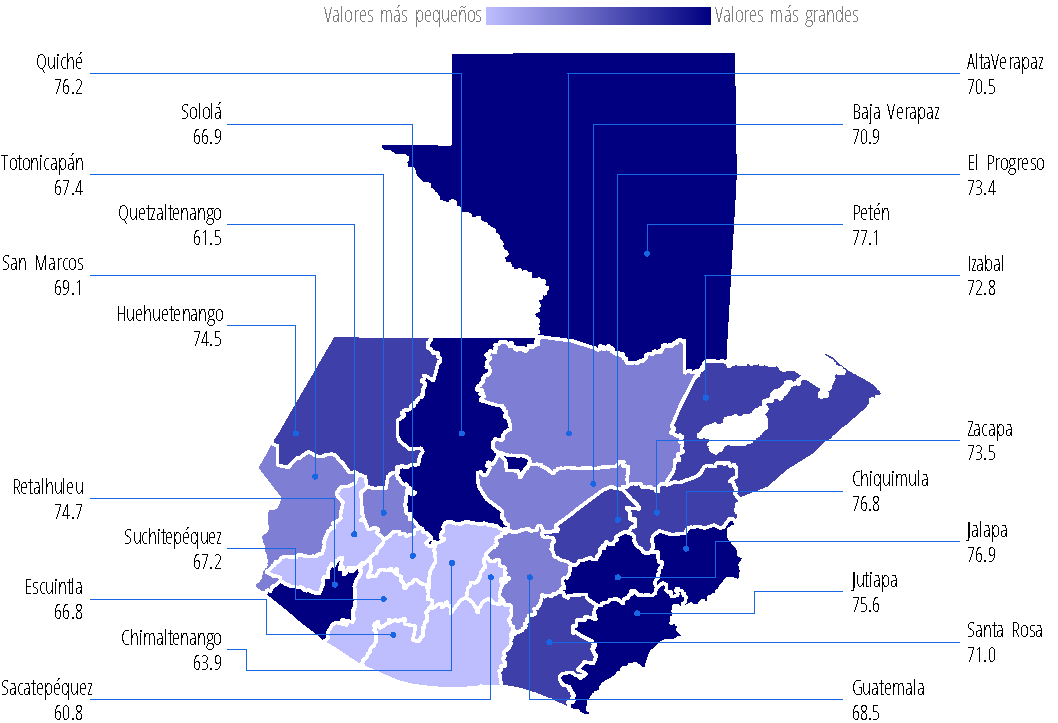
\includegraphics[width=52\cuadri]{graficas/basicos/1_25.pdf}}{Instituto Nacional de Estadística, con datos del Ministerio de Educación}




%
%
%\INEchaptercarta{Alumnos en diversificado}{}



\cajita{Inscritos en diversificado }{El número de  inscritos en diversificado, se obtiene a partir del total de los alumnos registrados al treinta de marzo de cada año escolar, que se inscriben en diversificado sin distinción de la edad
	
	 En el año 2009 se inscribieron 310,778 alumnos y en el año 2014 se inscribieron 396,461 alumnos, lo cual muestra un crecimiento de 27.6\%.}{Número de inscritos en el ciclo de educación diversificada}{República de Guatemala, serie histórica, en datos absolutos}{\ \\[0mm]\begin{tikzpicture}[x=1pt,y=1pt]  % Created by tikzDevice version 0.7.0 on 2015-08-28 13:12:26
% !TEX encoding = UTF-8 Unicode
\definecolor[named]{fillColor}{rgb}{1.00,1.00,1.00}
\path[use as bounding box,fill=fillColor,fill opacity=0.00] (0,0) rectangle (289.08,198.74);
\begin{scope}
\path[clip] (  0.00,  0.00) rectangle (289.08,198.74);
\definecolor[named]{drawColor}{rgb}{1.00,1.00,1.00}

\path[draw=drawColor,line width= 0.6pt,line join=round,line cap=round] (  0.00,  0.00) rectangle (289.08,198.74);
\end{scope}
\begin{scope}
\path[clip] (  0.00,  0.00) rectangle (289.08,198.74);

\path[] ( 14.70, 17.78) rectangle (280.54,191.48);

\path[] ( 14.70, 45.62) --
	(280.54, 45.62);

\path[] ( 14.70, 85.58) --
	(280.54, 85.58);

\path[] ( 14.70,125.54) --
	(280.54,125.54);

\path[] ( 14.70,165.49) --
	(280.54,165.49);

\path[] ( 14.70, 25.65) --
	(280.54, 25.65);

\path[] ( 14.70, 65.60) --
	(280.54, 65.60);

\path[] ( 14.70,105.56) --
	(280.54,105.56);

\path[] ( 14.70,145.51) --
	(280.54,145.51);

\path[] ( 14.70,185.47) --
	(280.54,185.47);

\path[] ( 45.37, 17.78) --
	( 45.37,191.48);

\path[] ( 96.50, 17.78) --
	( 96.50,191.48);

\path[] (147.62, 17.78) --
	(147.62,191.48);

\path[] (198.74, 17.78) --
	(198.74,191.48);

\path[] (249.87, 17.78) --
	(249.87,191.48);
\definecolor[named]{drawColor}{rgb}{0.00,0.00,1.00}

\path[draw=drawColor,line width= 1.7pt,line join=round] ( 45.37,149.82) --
	( 96.50,166.05) --
	(147.62,174.68) --
	(198.74,182.69) --
	(249.87,183.59);
\definecolor[named]{drawColor}{rgb}{0.00,0.00,0.00}

\node[text=drawColor,anchor=base,inner sep=0pt, outer sep=0pt, scale=  1.01] at ( 45.37,137.95) {310,778};

\node[text=drawColor,anchor=base east,inner sep=0pt, outer sep=0pt, scale=  1.01] at ( 90.72,166.05) {351,397};

\node[text=drawColor,anchor=base east,inner sep=0pt, outer sep=0pt, scale=  1.01] at (141.84,174.68) {373,004};

\node[text=drawColor,anchor=base east,inner sep=0pt, outer sep=0pt, scale=  1.01] at (192.97,182.69) {393,043};

\node[text=drawColor,anchor=base,inner sep=0pt, outer sep=0pt, scale=  1.01] at (249.87,187.54) {395,293};
\definecolor[named]{fillColor}{rgb}{0.00,0.00,0.00}

\path[draw=drawColor,line width= 0.1pt,line join=round,fill=fillColor] ( 14.70, 25.67) -- (280.54, 25.67);
\end{scope}
\begin{scope}
\path[clip] (  0.00,  0.00) rectangle (289.08,198.74);

\path[] ( 14.70, 17.78) --
	( 14.70,191.48);
\end{scope}
\begin{scope}
\path[clip] (  0.00,  0.00) rectangle (289.08,198.74);
\definecolor[named]{drawColor}{rgb}{1.00,1.00,1.00}

\node[text=drawColor,text opacity=0.00,anchor=base east,inner sep=0pt, outer sep=0pt, scale=  1.00] at (  7.58, 21.74) {0e+00};

\node[text=drawColor,text opacity=0.00,anchor=base east,inner sep=0pt, outer sep=0pt, scale=  1.00] at (  7.58, 61.69) {1e+05};

\node[text=drawColor,text opacity=0.00,anchor=base east,inner sep=0pt, outer sep=0pt, scale=  1.00] at (  7.58,101.65) {2e+05};

\node[text=drawColor,text opacity=0.00,anchor=base east,inner sep=0pt, outer sep=0pt, scale=  1.00] at (  7.58,141.60) {3e+05};

\node[text=drawColor,text opacity=0.00,anchor=base east,inner sep=0pt, outer sep=0pt, scale=  1.00] at (  7.58,181.56) {4e+05};
\end{scope}
\begin{scope}
\path[clip] (  0.00,  0.00) rectangle (289.08,198.74);

\path[] ( 10.43, 25.65) --
	( 14.70, 25.65);

\path[] ( 10.43, 65.60) --
	( 14.70, 65.60);

\path[] ( 10.43,105.56) --
	( 14.70,105.56);

\path[] ( 10.43,145.51) --
	( 14.70,145.51);

\path[] ( 10.43,185.47) --
	( 14.70,185.47);
\end{scope}
\begin{scope}
\path[clip] (  0.00,  0.00) rectangle (289.08,198.74);

\path[] ( 14.70, 17.78) --
	(280.54, 17.78);
\end{scope}
\begin{scope}
\path[clip] (  0.00,  0.00) rectangle (289.08,198.74);

\path[] ( 45.37, 13.51) --
	( 45.37, 17.78);

\path[] ( 96.50, 13.51) --
	( 96.50, 17.78);

\path[] (147.62, 13.51) --
	(147.62, 17.78);

\path[] (198.74, 13.51) --
	(198.74, 17.78);

\path[] (249.87, 13.51) --
	(249.87, 17.78);
\end{scope}
\begin{scope}
\path[clip] (  0.00,  0.00) rectangle (289.08,198.74);
\definecolor[named]{drawColor}{rgb}{0.00,0.00,0.00}

\node[text=drawColor,anchor=base,inner sep=0pt, outer sep=0pt, scale=  1.00] at ( 45.37,  2.85) {2009};

\node[text=drawColor,anchor=base,inner sep=0pt, outer sep=0pt, scale=  1.00] at ( 96.50,  2.85) {2010};

\node[text=drawColor,anchor=base,inner sep=0pt, outer sep=0pt, scale=  1.00] at (147.62,  2.85) {2011};

\node[text=drawColor,anchor=base,inner sep=0pt, outer sep=0pt, scale=  1.00] at (198.74,  2.85) {2012};

\node[text=drawColor,anchor=base,inner sep=0pt, outer sep=0pt, scale=  1.00] at (249.87,  2.85) {2014};
\end{scope}
  \end{tikzpicture}}{Instituto Nacional de Estadística, con datos del Ministerio de Educación}

\cajita{Inscritos en diversificado por sexo}{En la gráfica  se observa que el porcentaje de hombres inscritos en diversificado fue del 49.9\% y de mujeres 50.1\%.}{Distribución de inscritos en el ciclo de\\ educación diversificada, por sexo}{República de Guatemala, año 2014, en porcentaje}{\ \\[0mm]\begin{tikzpicture}[x=1pt,y=1pt]  % Created by tikzDevice version 0.10.1 on 2016-02-29 12:46:26
% !TEX encoding = UTF-8 Unicode
\definecolor{fillColor}{RGB}{255,255,255}
\path[use as bounding box,fill=fillColor,fill opacity=0.00] (0,0) rectangle (289.08,198.74);
\begin{scope}
\path[clip] ( 30.54,  0.00) rectangle (258.54,198.74);

\path[] ( 30.54,  0.00) rectangle (258.54,198.74);
\end{scope}
\begin{scope}
\path[clip] (  0.00,  0.00) rectangle (289.08,198.74);

\path[] (  7.11,  4.95) rectangle (200.91,198.74);

\path[] (104.01,101.85) --
	(191.22,101.49);

\path[] (104.01,101.85) --
	( 16.80,102.21);

\path[] (104.01,101.85) --
	(104.37,189.05);

\path[] (104.01,101.85) --
	(191.22,101.49);

\path[] (104.01,101.85) --
	(103.65, 14.64);

\path[] (104.01,101.85) --
	( 16.80,102.21);

\path[] (104.01,101.85) --
	(104.01,101.85) --
	(104.01,101.85) --
	(104.01,101.85) --
	(104.01,101.85) --
	(104.01,101.85) --
	(104.01,101.85) --
	(104.01,101.85) --
	(104.01,101.85) --
	(104.01,101.85) --
	(104.01,101.85) --
	(104.01,101.85) --
	(104.01,101.85) --
	(104.01,101.85) --
	(104.01,101.85) --
	(104.01,101.85) --
	(104.01,101.85) --
	(104.01,101.85) --
	(104.01,101.85) --
	(104.01,101.85) --
	(104.01,101.85) --
	(104.01,101.85) --
	(104.01,101.85) --
	(104.01,101.85) --
	(104.01,101.85) --
	(104.01,101.85) --
	(104.01,101.85) --
	(104.01,101.85) --
	(104.01,101.85) --
	(104.01,101.85) --
	(104.01,101.85) --
	(104.01,101.85) --
	(104.01,101.85) --
	(104.01,101.85) --
	(104.01,101.85) --
	(104.01,101.85) --
	(104.01,101.85) --
	(104.01,101.85) --
	(104.01,101.85) --
	(104.01,101.85) --
	(104.01,101.85) --
	(104.01,101.85) --
	(104.01,101.85) --
	(104.01,101.85) --
	(104.01,101.85) --
	(104.01,101.85) --
	(104.01,101.85) --
	(104.01,101.85) --
	(104.01,101.85) --
	(104.01,101.85) --
	(104.01,101.85) --
	(104.01,101.85) --
	(104.01,101.85) --
	(104.01,101.85) --
	(104.01,101.85) --
	(104.01,101.85) --
	(104.01,101.85) --
	(104.01,101.85) --
	(104.01,101.85) --
	(104.01,101.85) --
	(104.01,101.85) --
	(104.01,101.85) --
	(104.01,101.85) --
	(104.01,101.85) --
	(104.01,101.85) --
	(104.01,101.85) --
	(104.01,101.85) --
	(104.01,101.85) --
	(104.01,101.85) --
	(104.01,101.85) --
	(104.01,101.85) --
	(104.01,101.85) --
	(104.01,101.85) --
	(104.01,101.85) --
	(104.01,101.85) --
	(104.01,101.85) --
	(104.01,101.85) --
	(104.01,101.85) --
	(104.01,101.85) --
	(104.01,101.85) --
	(104.01,101.85) --
	(104.01,101.85) --
	(104.01,101.85) --
	(104.01,101.85) --
	(104.01,101.85) --
	(104.01,101.85) --
	(104.01,101.85) --
	(104.01,101.85) --
	(104.01,101.85) --
	(104.01,101.85) --
	(104.01,101.85) --
	(104.01,101.85) --
	(104.01,101.85) --
	(104.01,101.85) --
	(104.01,101.85) --
	(104.01,101.85) --
	(104.01,101.85) --
	(104.01,101.85) --
	(104.01,101.85) --
	(104.01,101.85);

\path[] (104.01,121.23) --
	(105.24,121.19) --
	(106.46,121.07) --
	(107.68,120.88) --
	(108.88,120.60) --
	(110.06,120.26) --
	(111.21,119.84) --
	(112.34,119.34) --
	(113.43,118.78) --
	(114.49,118.15) --
	(115.50,117.45) --
	(116.47,116.69) --
	(117.38,115.87) --
	(118.25,115.00) --
	(119.05,114.07) --
	(119.80,113.09) --
	(120.48,112.06) --
	(121.09,111.00) --
	(121.64,109.90) --
	(122.11,108.76) --
	(122.51,107.60) --
	(122.84,106.42) --
	(123.09,105.21) --
	(123.27,103.99) --
	(123.37,102.77) --
	(123.39,101.54) --
	(123.33,100.31) --
	(123.19, 99.09) --
	(122.98, 97.88) --
	(122.69, 96.68) --
	(122.32, 95.51) --
	(121.88, 94.36) --
	(121.37, 93.24) --
	(120.79, 92.16) --
	(120.14, 91.11) --
	(119.43, 90.11) --
	(118.66, 89.16) --
	(117.82, 88.25) --
	(116.93, 87.40) --
	(115.99, 86.61) --
	(115.00, 85.88) --
	(113.96, 85.22) --
	(112.89, 84.62) --
	(111.78, 84.09) --
	(110.64, 83.64) --
	(109.47, 83.25) --
	(108.28, 82.94) --
	(107.07, 82.71) --
	(105.85, 82.55) --
	(104.62, 82.48) --
	(103.39, 82.48) --
	(102.17, 82.55) --
	(100.95, 82.71) --
	( 99.74, 82.94) --
	( 98.55, 83.25) --
	( 97.38, 83.64) --
	( 96.24, 84.09) --
	( 95.13, 84.62) --
	( 94.05, 85.22) --
	( 93.02, 85.88) --
	( 92.03, 86.61) --
	( 91.09, 87.40) --
	( 90.20, 88.25) --
	( 89.36, 89.16) --
	( 88.59, 90.11) --
	( 87.87, 91.11) --
	( 87.23, 92.16) --
	( 86.65, 93.24) --
	( 86.13, 94.36) --
	( 85.70, 95.51) --
	( 85.33, 96.68) --
	( 85.04, 97.88) --
	( 84.83, 99.09) --
	( 84.69,100.31) --
	( 84.63,101.54) --
	( 84.65,102.77) --
	( 84.75,103.99) --
	( 84.92,105.21) --
	( 85.18,106.42) --
	( 85.50,107.60) --
	( 85.91,108.76) --
	( 86.38,109.90) --
	( 86.93,111.00) --
	( 87.54,112.06) --
	( 88.22,113.09) --
	( 88.97,114.07) --
	( 89.77,115.00) --
	( 90.64,115.87) --
	( 91.55,116.69) --
	( 92.52,117.45) --
	( 93.53,118.15) --
	( 94.59,118.78) --
	( 95.68,119.34) --
	( 96.81,119.84) --
	( 97.96,120.26) --
	( 99.14,120.60) --
	(100.34,120.88) --
	(101.56,121.07) --
	(102.78,121.19) --
	(104.01,121.23);

\path[] (104.01,140.60) --
	(106.47,140.53) --
	(108.92,140.29) --
	(111.34,139.90) --
	(113.74,139.36) --
	(116.10,138.67) --
	(118.41,137.83) --
	(120.67,136.84) --
	(122.85,135.72) --
	(124.96,134.45) --
	(126.99,133.06) --
	(128.92,131.54) --
	(130.76,129.90) --
	(132.48,128.14) --
	(134.09,126.29) --
	(135.58,124.33) --
	(136.94,122.28) --
	(138.17,120.15) --
	(139.27,117.95) --
	(140.22,115.68) --
	(141.02,113.35) --
	(141.68,110.98) --
	(142.18,108.58) --
	(142.53,106.14) --
	(142.72,103.69) --
	(142.76,101.23) --
	(142.65, 98.77) --
	(142.37, 96.33) --
	(141.95, 93.91) --
	(141.37, 91.52) --
	(140.64, 89.17) --
	(139.76, 86.87) --
	(138.74, 84.63) --
	(137.58, 82.47) --
	(136.28, 80.38) --
	(134.85, 78.37) --
	(133.30, 76.46) --
	(131.63, 74.66) --
	(129.85, 72.96) --
	(127.97, 71.38) --
	(125.99, 69.92) --
	(123.92, 68.59) --
	(121.77, 67.40) --
	(119.55, 66.34) --
	(117.27, 65.43) --
	(114.93, 64.66) --
	(112.55, 64.04) --
	(110.13, 63.57) --
	(107.69, 63.26) --
	(105.24, 63.11) --
	(102.78, 63.11) --
	(100.33, 63.26) --
	( 97.89, 63.57) --
	( 95.47, 64.04) --
	( 93.09, 64.66) --
	( 90.75, 65.43) --
	( 88.47, 66.34) --
	( 86.25, 67.40) --
	( 84.10, 68.59) --
	( 82.03, 69.92) --
	( 80.05, 71.38) --
	( 78.17, 72.96) --
	( 76.39, 74.66) --
	( 74.72, 76.46) --
	( 73.17, 78.37) --
	( 71.74, 80.38) --
	( 70.44, 82.47) --
	( 69.28, 84.63) --
	( 68.26, 86.87) --
	( 67.38, 89.17) --
	( 66.65, 91.52) --
	( 66.07, 93.91) --
	( 65.65, 96.33) --
	( 65.37, 98.77) --
	( 65.26,101.23) --
	( 65.29,103.69) --
	( 65.49,106.14) --
	( 65.84,108.58) --
	( 66.34,110.98) --
	( 67.00,113.35) --
	( 67.80,115.68) --
	( 68.75,117.95) --
	( 69.85,120.15) --
	( 71.08,122.28) --
	( 72.44,124.33) --
	( 73.93,126.29) --
	( 75.54,128.14) --
	( 77.26,129.90) --
	( 79.10,131.54) --
	( 81.03,133.06) --
	( 83.06,134.45) --
	( 85.17,135.72) --
	( 87.35,136.84) --
	( 89.60,137.83) --
	( 91.92,138.67) --
	( 94.28,139.36) --
	( 96.67,139.90) --
	( 99.10,140.29) --
	(101.55,140.53) --
	(104.01,140.60);

\path[] (104.01,159.98) --
	(107.70,159.87) --
	(111.37,159.52) --
	(115.01,158.93) --
	(118.61,158.12) --
	(122.15,157.08) --
	(125.62,155.82) --
	(129.00,154.34) --
	(132.28,152.65) --
	(135.44,150.75) --
	(138.48,148.66) --
	(141.38,146.38) --
	(144.13,143.92) --
	(146.72,141.29) --
	(149.13,138.51) --
	(151.37,135.57) --
	(153.41,132.50) --
	(155.26,129.30) --
	(156.89,126.00) --
	(158.32,122.59) --
	(159.53,119.11) --
	(160.51,115.55) --
	(161.26,111.94) --
	(161.79,108.29) --
	(162.08,104.61) --
	(162.14,100.92) --
	(161.96, 97.24) --
	(161.56, 93.57) --
	(160.91, 89.94) --
	(160.05, 86.35) --
	(158.95, 82.83) --
	(157.63, 79.39) --
	(156.10, 76.03) --
	(154.36, 72.78) --
	(152.41, 69.64) --
	(150.27, 66.64) --
	(147.95, 63.77) --
	(145.44, 61.06) --
	(142.77, 58.52) --
	(139.95, 56.15) --
	(136.98, 53.96) --
	(133.87, 51.97) --
	(130.65, 50.17) --
	(127.32, 48.59) --
	(123.89, 47.21) --
	(120.39, 46.06) --
	(116.82, 45.14) --
	(113.20, 44.44) --
	(109.54, 43.97) --
	(105.85, 43.74) --
	(102.16, 43.74) --
	( 98.48, 43.97) --
	( 94.82, 44.44) --
	( 91.20, 45.14) --
	( 87.63, 46.06) --
	( 84.13, 47.21) --
	( 80.70, 48.59) --
	( 77.37, 50.17) --
	( 74.15, 51.97) --
	( 71.04, 53.96) --
	( 68.07, 56.15) --
	( 65.25, 58.52) --
	( 62.58, 61.06) --
	( 60.07, 63.77) --
	( 57.75, 66.64) --
	( 55.61, 69.64) --
	( 53.66, 72.78) --
	( 51.92, 76.03) --
	( 50.39, 79.39) --
	( 49.07, 82.83) --
	( 47.97, 86.35) --
	( 47.10, 89.94) --
	( 46.46, 93.57) --
	( 46.05, 97.24) --
	( 45.88,100.92) --
	( 45.94,104.61) --
	( 46.23,108.29) --
	( 46.75,111.94) --
	( 47.51,115.55) --
	( 48.49,119.11) --
	( 49.70,122.59) --
	( 51.13,126.00) --
	( 52.76,129.30) --
	( 54.61,132.50) --
	( 56.65,135.57) --
	( 58.89,138.51) --
	( 61.30,141.29) --
	( 63.89,143.92) --
	( 66.64,146.38) --
	( 69.54,148.66) --
	( 72.58,150.75) --
	( 75.74,152.65) --
	( 79.02,154.34) --
	( 82.40,155.82) --
	( 85.87,157.08) --
	( 89.41,158.12) --
	( 93.01,158.93) --
	( 96.65,159.52) --
	(100.32,159.87) --
	(104.01,159.98);

\path[] (104.01,179.36) --
	(108.93,179.21) --
	(113.82,178.74) --
	(118.68,177.96) --
	(123.48,176.88) --
	(128.20,175.49) --
	(132.82,173.81) --
	(137.33,171.84) --
	(141.70,169.58) --
	(145.92,167.06) --
	(149.97,164.27) --
	(153.84,161.23) --
	(157.50,157.95) --
	(160.95,154.44) --
	(164.17,150.72) --
	(167.15,146.81) --
	(169.88,142.72) --
	(172.34,138.46) --
	(174.52,134.05) --
	(176.42,129.51) --
	(178.03,124.86) --
	(179.34,120.12) --
	(180.35,115.31) --
	(181.05,110.44) --
	(181.44,105.53) --
	(181.52,100.62) --
	(181.28, 95.70) --
	(180.74, 90.81) --
	(179.88, 85.97) --
	(178.72, 81.19) --
	(177.26, 76.49) --
	(175.51, 71.90) --
	(173.46, 67.42) --
	(171.14, 63.09) --
	(168.55, 58.91) --
	(165.69, 54.90) --
	(162.59, 51.08) --
	(159.26, 47.47) --
	(155.70, 44.08) --
	(151.93, 40.91) --
	(147.97, 38.00) --
	(143.83, 35.34) --
	(139.53, 32.95) --
	(135.09, 30.83) --
	(130.52, 29.00) --
	(125.85, 27.47) --
	(121.09, 26.23) --
	(116.26, 25.30) --
	(111.38, 24.68) --
	(106.47, 24.37) --
	(101.55, 24.37) --
	( 96.64, 24.68) --
	( 91.76, 25.30) --
	( 86.93, 26.23) --
	( 82.17, 27.47) --
	( 77.50, 29.00) --
	( 72.93, 30.83) --
	( 68.49, 32.95) --
	( 64.19, 35.34) --
	( 60.05, 38.00) --
	( 56.09, 40.91) --
	( 52.32, 44.08) --
	( 48.76, 47.47) --
	( 45.43, 51.08) --
	( 42.32, 54.90) --
	( 39.47, 58.91) --
	( 36.88, 63.09) --
	( 34.55, 67.42) --
	( 32.51, 71.90) --
	( 30.76, 76.49) --
	( 29.30, 81.19) --
	( 28.14, 85.97) --
	( 27.28, 90.81) --
	( 26.74, 95.70) --
	( 26.50,100.62) --
	( 26.58,105.53) --
	( 26.97,110.44) --
	( 27.67,115.31) --
	( 28.68,120.12) --
	( 29.99,124.86) --
	( 31.60,129.51) --
	( 33.50,134.05) --
	( 35.68,138.46) --
	( 38.14,142.72) --
	( 40.87,146.81) --
	( 43.84,150.72) --
	( 47.07,154.44) --
	( 50.52,157.95) --
	( 54.18,161.23) --
	( 58.05,164.27) --
	( 62.10,167.06) --
	( 66.32,169.58) --
	( 70.69,171.84) --
	( 75.20,173.81) --
	( 79.82,175.49) --
	( 84.54,176.88) --
	( 89.34,177.96) --
	( 94.20,178.74) --
	( 99.09,179.21) --
	(104.01,179.36);

\path[] (104.01,189.05) --
	(109.54,188.88) --
	(115.05,188.35) --
	(120.51,187.48) --
	(125.91,186.26) --
	(131.22,184.70) --
	(136.42,182.81) --
	(141.49,180.59) --
	(146.41,178.05) --
	(151.16,175.21) --
	(155.71,172.07) --
	(160.06,168.65) --
	(164.19,164.96) --
	(168.07,161.02) --
	(171.69,156.83) --
	(175.05,152.43) --
	(178.11,147.82) --
	(180.88,143.03) --
	(183.34,138.07) --
	(185.47,132.97) --
	(187.28,127.74) --
	(188.76,122.41) --
	(189.89,116.99) --
	(190.68,111.51) --
	(191.12,106.00) --
	(191.21,100.46) --
	(190.94, 94.94) --
	(190.33, 89.44) --
	(189.37, 83.99) --
	(188.06, 78.61) --
	(186.42, 73.32) --
	(184.44, 68.15) --
	(182.15, 63.12) --
	(179.53, 58.24) --
	(176.62, 53.54) --
	(173.41, 49.03) --
	(169.92, 44.74) --
	(166.16, 40.67) --
	(162.16, 36.85) --
	(157.92, 33.30) --
	(153.46, 30.02) --
	(148.81, 27.02) --
	(143.97, 24.33) --
	(138.97, 21.96) --
	(133.84, 19.90) --
	(128.58, 18.17) --
	(123.22, 16.78) --
	(117.79, 15.74) --
	(112.30, 15.03) --
	(106.78, 14.68) --
	(101.24, 14.68) --
	( 95.72, 15.03) --
	( 90.23, 15.74) --
	( 84.80, 16.78) --
	( 79.44, 18.17) --
	( 74.18, 19.90) --
	( 69.05, 21.96) --
	( 64.05, 24.33) --
	( 59.21, 27.02) --
	( 54.56, 30.02) --
	( 50.10, 33.30) --
	( 45.86, 36.85) --
	( 41.86, 40.67) --
	( 38.10, 44.74) --
	( 34.61, 49.03) --
	( 31.40, 53.54) --
	( 28.49, 58.24) --
	( 25.87, 63.12) --
	( 23.57, 68.15) --
	( 21.60, 73.32) --
	( 19.96, 78.61) --
	( 18.65, 83.99) --
	( 17.69, 89.44) --
	( 17.08, 94.94) --
	( 16.81,100.46) --
	( 16.90,106.00) --
	( 17.34,111.51) --
	( 18.13,116.99) --
	( 19.26,122.41) --
	( 20.74,127.74) --
	( 22.55,132.97) --
	( 24.68,138.07) --
	( 27.14,143.03) --
	( 29.91,147.82) --
	( 32.97,152.43) --
	( 36.32,156.83) --
	( 39.95,161.02) --
	( 43.83,164.96) --
	( 47.95,168.65) --
	( 52.30,172.07) --
	( 56.86,175.21) --
	( 61.61,178.05) --
	( 66.53,180.59) --
	( 71.60,182.81) --
	( 76.80,184.70) --
	( 82.11,186.26) --
	( 87.51,187.48) --
	( 92.97,188.35) --
	( 98.48,188.88) --
	(104.01,189.05);
\definecolor{drawColor}{RGB}{255,255,255}
\definecolor{fillColor}{RGB}{0,0,255}

\path[draw=drawColor,line width= 0.6pt,line join=round,line cap=round,fill=fillColor] (103.69, 63.09) --
	(103.67, 60.32) --
	(103.64, 57.55) --
	(103.62, 54.78) --
	(103.60, 52.02) --
	(103.57, 49.25) --
	(103.55, 46.48) --
	(103.53, 43.71) --
	(103.51, 40.94) --
	(103.48, 38.17) --
	(103.46, 35.41) --
	(103.44, 32.64) --
	(103.41, 29.87) --
	(103.39, 27.10) --
	(103.37, 24.33) --
	(105.99, 24.35) --
	(108.62, 24.47) --
	(111.23, 24.67) --
	(113.84, 24.96) --
	(116.44, 25.33) --
	(119.02, 25.80) --
	(121.59, 26.35) --
	(124.14, 26.99) --
	(126.66, 27.71) --
	(129.16, 28.52) --
	(131.63, 29.42) --
	(134.06, 30.39) --
	(136.47, 31.45) --
	(138.83, 32.59) --
	(141.16, 33.81) --
	(143.44, 35.11) --
	(145.68, 36.48) --
	(147.87, 37.93) --
	(150.01, 39.45) --
	(152.09, 41.04) --
	(154.12, 42.71) --
	(156.10, 44.44) --
	(158.01, 46.23) --
	(159.86, 48.10) --
	(161.65, 50.02) --
	(163.37, 52.00) --
	(165.03, 54.04) --
	(166.61, 56.13) --
	(168.12, 58.28) --
	(169.56, 60.47) --
	(170.93, 62.72) --
	(172.21, 65.01) --
	(173.42, 67.34) --
	(174.55, 69.71) --
	(175.60, 72.11) --
	(176.56, 74.56) --
	(177.45, 77.03) --
	(178.24, 79.53) --
	(178.96, 82.06) --
	(179.58, 84.61) --
	(180.13, 87.17) --
	(180.58, 89.76) --
	(180.94, 92.36) --
	(181.22, 94.97) --
	(181.41, 97.59) --
	(181.51,100.21) --
	(181.52,102.84) --
	(181.44,105.46) --
	(181.28,108.08) --
	(181.02,110.70) --
	(180.68,113.30) --
	(180.24,115.89) --
	(179.72,118.46) --
	(179.12,121.02) --
	(178.43,123.55) --
	(177.65,126.06) --
	(176.79,128.54) --
	(175.84,130.98) --
	(174.81,133.40) --
	(173.70,135.78) --
	(172.52,138.12) --
	(171.25,140.42) --
	(169.90,142.67) --
	(168.48,144.88) --
	(166.99,147.04) --
	(165.42,149.15) --
	(163.78,151.20) --
	(162.08,153.20) --
	(160.31,155.13) --
	(158.47,157.01) --
	(156.57,158.82) --
	(154.61,160.57) --
	(152.59,162.25) --
	(150.52,163.86) --
	(148.39,165.40) --
	(146.22,166.86) --
	(143.99,168.26) --
	(141.72,169.57) --
	(139.40,170.81) --
	(137.05,171.97) --
	(134.65,173.05) --
	(132.23,174.05) --
	(129.77,174.96) --
	(127.27,175.79) --
	(124.76,176.54) --
	(122.22,177.19) --
	(119.65,177.77) --
	(117.07,178.25) --
	(114.48,178.65) --
	(111.87,178.96) --
	(109.26,179.19) --
	(106.63,179.32) --
	(104.01,179.36) --
	(104.01,176.59) --
	(104.01,173.83) --
	(104.01,171.06) --
	(104.01,168.29) --
	(104.01,165.52) --
	(104.01,162.75) --
	(104.01,159.98) --
	(104.01,157.22) --
	(104.01,154.45) --
	(104.01,151.68) --
	(104.01,148.91) --
	(104.01,146.14) --
	(104.01,143.37) --
	(104.01,140.60) --
	(106.66,140.51) --
	(109.30,140.24) --
	(111.92,139.79) --
	(114.49,139.16) --
	(117.02,138.36) --
	(119.49,137.38) --
	(121.88,136.24) --
	(124.20,134.93) --
	(126.41,133.47) --
	(128.52,131.87) --
	(130.52,130.12) --
	(132.39,128.24) --
	(134.13,126.24) --
	(135.73,124.12) --
	(137.18,121.90) --
	(138.47,119.58) --
	(139.61,117.18) --
	(140.57,114.71) --
	(141.37,112.18) --
	(141.99,109.60) --
	(142.43,106.98) --
	(142.69,104.34) --
	(142.77,101.69) --
	(142.67, 99.03) --
	(142.38, 96.40) --
	(141.92, 93.78) --
	(141.28, 91.21) --
	(140.46, 88.68) --
	(139.48, 86.22) --
	(138.33, 83.83) --
	(137.01, 81.52) --
	(135.54, 79.31) --
	(133.93, 77.21) --
	(132.17, 75.22) --
	(130.29, 73.35) --
	(128.27, 71.62) --
	(126.15, 70.03) --
	(123.92, 68.59) --
	(121.60, 67.31) --
	(119.19, 66.19) --
	(116.72, 65.23) --
	(114.18, 64.45) --
	(111.60, 63.84) --
	(108.98, 63.41) --
	(106.34, 63.16) --
	(103.69, 63.09) --
	cycle;
\definecolor{fillColor}{RGB}{157,187,255}

\path[draw=drawColor,line width= 0.6pt,line join=round,line cap=round,fill=fillColor] (104.01,140.60) --
	(104.01,143.37) --
	(104.01,146.14) --
	(104.01,148.91) --
	(104.01,151.68) --
	(104.01,154.45) --
	(104.01,157.22) --
	(104.01,159.98) --
	(104.01,162.75) --
	(104.01,165.52) --
	(104.01,168.29) --
	(104.01,171.06) --
	(104.01,173.83) --
	(104.01,176.59) --
	(104.01,179.36) --
	(101.37,179.32) --
	( 98.73,179.18) --
	( 96.10,178.96) --
	( 93.48,178.65) --
	( 90.87,178.24) --
	( 88.28,177.75) --
	( 85.70,177.17) --
	( 83.15,176.50) --
	( 80.62,175.75) --
	( 78.12,174.91) --
	( 75.64,173.99) --
	( 73.20,172.98) --
	( 70.80,171.89) --
	( 68.43,170.72) --
	( 66.11,169.47) --
	( 63.83,168.14) --
	( 61.59,166.73) --
	( 59.41,165.25) --
	( 57.28,163.69) --
	( 55.20,162.07) --
	( 53.18,160.37) --
	( 51.21,158.60) --
	( 49.31,156.77) --
	( 47.47,154.88) --
	( 45.70,152.92) --
	( 43.99,150.91) --
	( 42.36,148.83) --
	( 40.79,146.71) --
	( 39.30,144.53) --
	( 37.89,142.30) --
	( 36.55,140.03) --
	( 35.29,137.71) --
	( 34.11,135.35) --
	( 33.00,132.95) --
	( 31.99,130.51) --
	( 31.05,128.04) --
	( 30.20,125.54) --
	( 29.44,123.02) --
	( 28.76,120.46) --
	( 28.17,117.89) --
	( 27.67,115.30) --
	( 27.25,112.69) --
	( 26.93,110.07) --
	( 26.69,107.44) --
	( 26.55,104.81) --
	( 26.49,102.17) --
	( 26.53, 99.53) --
	( 26.65, 96.89) --
	( 26.86, 94.26) --
	( 27.17, 91.64) --
	( 27.56, 89.03) --
	( 28.04, 86.43) --
	( 28.61, 83.85) --
	( 29.27, 81.30) --
	( 30.01, 78.76) --
	( 30.84, 76.26) --
	( 31.75, 73.78) --
	( 32.75, 71.33) --
	( 33.83, 68.93) --
	( 34.99, 66.56) --
	( 36.23, 64.23) --
	( 37.55, 61.94) --
	( 38.95, 59.70) --
	( 40.42, 57.51) --
	( 41.97, 55.37) --
	( 43.59, 53.28) --
	( 45.28, 51.26) --
	( 47.03, 49.28) --
	( 48.86, 47.37) --
	( 50.74, 45.53) --
	( 52.69, 43.75) --
	( 54.70, 42.03) --
	( 56.77, 40.39) --
	( 58.89, 38.82) --
	( 61.06, 37.32) --
	( 63.28, 35.89) --
	( 65.55, 34.54) --
	( 67.86, 33.27) --
	( 70.22, 32.08) --
	( 72.62, 30.97) --
	( 75.05, 29.94) --
	( 77.51, 29.00) --
	( 80.01, 28.14) --
	( 82.53, 27.36) --
	( 85.08, 26.68) --
	( 87.65, 26.07) --
	( 90.24, 25.56) --
	( 92.85, 25.14) --
	( 95.46, 24.80) --
	( 98.09, 24.56) --
	(100.73, 24.40) --
	(103.37, 24.33) --
	(103.39, 27.10) --
	(103.41, 29.87) --
	(103.44, 32.64) --
	(103.46, 35.41) --
	(103.48, 38.17) --
	(103.51, 40.94) --
	(103.53, 43.71) --
	(103.55, 46.48) --
	(103.57, 49.25) --
	(103.60, 52.02) --
	(103.62, 54.78) --
	(103.64, 57.55) --
	(103.67, 60.32) --
	(103.69, 63.09) --
	(101.05, 63.20) --
	( 98.43, 63.49) --
	( 95.83, 63.96) --
	( 93.27, 64.61) --
	( 90.76, 65.42) --
	( 88.31, 66.41) --
	( 85.94, 67.56) --
	( 83.65, 68.87) --
	( 81.45, 70.33) --
	( 79.36, 71.94) --
	( 77.38, 73.69) --
	( 75.52, 75.57) --
	( 73.80, 77.57) --
	( 72.22, 79.68) --
	( 70.78, 81.89) --
	( 69.50, 84.20) --
	( 68.38, 86.59) --
	( 67.42, 89.05) --
	( 66.64, 91.57) --
	( 66.03, 94.14) --
	( 65.59, 96.74) --
	( 65.33, 99.37) --
	( 65.25,102.01) --
	( 65.35,104.64) --
	( 65.63,107.27) --
	( 66.09,109.87) --
	( 66.72,112.43) --
	( 67.53,114.94) --
	( 68.51,117.40) --
	( 69.65,119.78) --
	( 70.95,122.07) --
	( 72.40,124.28) --
	( 74.00,126.38) --
	( 75.74,128.36) --
	( 77.61,130.22) --
	( 79.60,131.96) --
	( 81.71,133.55) --
	( 83.92,134.99) --
	( 86.22,136.28) --
	( 88.61,137.41) --
	( 91.06,138.38) --
	( 93.58,139.17) --
	( 96.14,139.80) --
	( 98.75,140.25) --
	(101.37,140.51) --
	(104.01,140.60) --
	cycle;
\definecolor{drawColor}{RGB}{0,0,0}

\node[text=drawColor,anchor=base,inner sep=0pt, outer sep=0pt, scale=  1.00] at (191.22, 97.58) {50.1};

\node[text=drawColor,anchor=base,inner sep=0pt, outer sep=0pt, scale=  1.00] at ( 16.80, 98.30) {49.9};

\path[] (  7.11,  4.95) rectangle (200.91,198.74);
\end{scope}
\begin{scope}
\path[clip] (  0.00,  0.00) rectangle (289.08,198.74);

\path[] (  7.11,  4.95) --
	(  7.11,198.74);
\end{scope}
\begin{scope}
\path[clip] (  0.00,  0.00) rectangle (289.08,198.74);

\path[] (  4.36,101.85) --
	(  7.11,101.85);

\path[] (  4.36,121.23) --
	(  7.11,121.23);

\path[] (  4.36,140.60) --
	(  7.11,140.60);

\path[] (  4.36,159.98) --
	(  7.11,159.98);

\path[] (  4.36,179.36) --
	(  7.11,179.36);
\end{scope}
\begin{scope}
\path[clip] (  0.00,  0.00) rectangle (289.08,198.74);

\path[] (  7.11,  4.95) --
	(200.91,  4.95);
\end{scope}
\begin{scope}
\path[clip] (  0.00,  0.00) rectangle (289.08,198.74);
\coordinate (rect) at (192.72,99.37);
\coordinate (desY) at (0,18.49);
\coordinate (desX) at (7.11,11.38);
\coordinate (mdesX) at (7.11,-11.38);
\definecolor[named]{ct1}{HTML}{
0000FF
}
\definecolor[named]{borde}{HTML}{
0000FF
}
\coordinate (t1) at ($(rect) + 0.5*(desX) + 0.5*(desY)$);
\coordinate (t2) at ($(rect)+0.5*(mdesX)-0.5*(desY)$);
\draw [color=ct1,fill=borde] ($(rect)+(desY)$) rectangle ($(rect)+(desX)$);
\definecolor[named]{ct2}{HTML}{
9DBBFF
}
\node [text width=
56.692913328
,right= 0.3cm of t1,scale = 0.9]{
Mujer
};
\path [fill=ct2] ($(rect)-(desY)$) rectangle ($(rect)+(mdesX)$);
\node [text width=
56.692913328
,right= 0.3cm of t2,scale = 0.9]{
Hombre
};
\end{scope}
  \end{tikzpicture}}{Instituto Nacional de Estadística, con datos del Ministerio de Educación}

\cajita{Inscritos en diversificado por grado}{En la gráfica  se observa el número de inscritos por grado en diversificado  donde se concentra la mayor cantidad de alumnos fue en cuarto grado con el 39.6\%. El 0.2\% de los alumnos inscritos en diversificado ingresaron a séptimo grado de este ciclo.}{Distribución de inscritos en el ciclo de educación diversificada, según el grado escolar}{República de Guatemala, año 2014, en porcentaje}{\ \\[0mm]\begin{tikzpicture}[x=1pt,y=1pt]  % Created by tikzDevice version 0.7.0 on 2015-09-08 18:11:49
% !TEX encoding = UTF-8 Unicode
\definecolor[named]{fillColor}{rgb}{1.00,1.00,1.00}
\path[use as bounding box,fill=fillColor,fill opacity=0.00] (0,0) rectangle (289.08,198.74);
\begin{scope}
\path[clip] (  0.00,  0.00) rectangle (289.08,198.74);
\definecolor[named]{drawColor}{rgb}{1.00,1.00,1.00}

\path[draw=drawColor,line width= 0.6pt,line join=round,line cap=round] (  0.00,  0.00) rectangle (289.08,198.74);
\end{scope}
\begin{scope}
\path[clip] (  0.00,  0.00) rectangle (289.08,198.74);

\path[] (  7.11, 23.47) rectangle (289.08,181.67);

\path[] ( 47.39, 23.47) --
	( 47.39,181.67);

\path[] (114.53, 23.47) --
	(114.53,181.67);

\path[] (181.66, 23.47) --
	(181.66,181.67);

\path[] (248.80, 23.47) --
	(248.80,181.67);
\definecolor[named]{drawColor}{rgb}{0.00,0.00,1.00}
\definecolor[named]{fillColor}{rgb}{0.00,0.00,1.00}

\path[draw=drawColor,line width= 0.6pt,line join=round,fill=fillColor] ( 28.93, 23.47) rectangle ( 65.86,181.67);

\path[draw=drawColor,line width= 0.6pt,line join=round,fill=fillColor] ( 96.07, 23.47) rectangle (132.99,178.08);

\path[draw=drawColor,line width= 0.6pt,line join=round,fill=fillColor] (163.20, 23.47) rectangle (200.13,104.60);

\path[draw=drawColor,line width= 0.6pt,line join=round,fill=fillColor] (230.34, 23.47) rectangle (267.26, 24.06);
\definecolor[named]{drawColor}{rgb}{0.00,0.00,0.00}
\definecolor[named]{fillColor}{rgb}{0.00,0.00,0.00}

\path[draw=drawColor,line width= 0.1pt,line join=round,fill=fillColor] (  7.11, 23.47) -- (289.08, 23.47);

\node[text=drawColor,anchor=base,inner sep=0pt, outer sep=0pt, scale=  1.01] at ( 47.39,185.63) {40.1};

\node[text=drawColor,anchor=base,inner sep=0pt, outer sep=0pt, scale=  1.01] at (114.53,182.04) {39.2};

\node[text=drawColor,anchor=base,inner sep=0pt, outer sep=0pt, scale=  1.01] at (181.66,108.55) {20.6};

\node[text=drawColor,anchor=base,inner sep=0pt, outer sep=0pt, scale=  1.01] at (248.80, 28.02) {0.2};
\end{scope}
\begin{scope}
\path[clip] (  0.00,  0.00) rectangle (289.08,198.74);

\path[] (  7.11, 23.47) --
	(  7.11,181.67);
\end{scope}
\begin{scope}
\path[clip] (  0.00,  0.00) rectangle (289.08,198.74);

\path[] (  7.11, 23.47) --
	(289.08, 23.47);
\end{scope}
\begin{scope}
\path[clip] (  0.00,  0.00) rectangle (289.08,198.74);

\path[] ( 47.39, 19.20) --
	( 47.39, 23.47);

\path[] (114.53, 19.20) --
	(114.53, 23.47);

\path[] (181.66, 19.20) --
	(181.66, 23.47);

\path[] (248.80, 19.20) --
	(248.80, 23.47);
\end{scope}
\begin{scope}
\path[clip] (  0.00,  0.00) rectangle (289.08,198.74);
\definecolor[named]{drawColor}{rgb}{0.00,0.00,0.00}

\node[text=drawColor,anchor=base,inner sep=0pt, outer sep=0pt, scale=  1.00] at ( 47.39,  8.54) {Cuarto};

\node[text=drawColor,anchor=base,inner sep=0pt, outer sep=0pt, scale=  1.00] at (114.53,  8.54) {Quinto };

\node[text=drawColor,anchor=base,inner sep=0pt, outer sep=0pt, scale=  1.00] at (181.66,  8.54) {Sexto };

\node[text=drawColor,anchor=base,inner sep=0pt, outer sep=0pt, scale=  1.00] at (248.80,  8.54) {S\'eptimo};
\end{scope}
  \end{tikzpicture}}{Instituto Nacional de Estadística, con datos del Ministerio de Educación}

\cajita{Inscritos en diversificado por etnia}{En la gráfica  se observa que del total de inscritos en diversificado, los no indígenas representaron el 83.7\%.
	
	De cada 10 alumnos inscritos en educación diversificada 2 se autoidentificaban como indígenas.}{Distribución de inscritos en el ciclo de educación\\ diversificada, por grupo étnico}{República de Guatemala, año 2014, en porcentaje}{\ \\[0mm]\begin{tikzpicture}[x=1pt,y=1pt]  % Created by tikzDevice version 0.10.1 on 2016-02-29 12:46:45
% !TEX encoding = UTF-8 Unicode
\definecolor{fillColor}{RGB}{255,255,255}
\path[use as bounding box,fill=fillColor,fill opacity=0.00] (0,0) rectangle (289.08,198.74);
\begin{scope}
\path[clip] ( 30.54,  0.00) rectangle (258.54,198.74);

\path[] ( 30.54,  0.00) rectangle (258.54,198.74);
\end{scope}
\begin{scope}
\path[clip] (  0.00,  0.00) rectangle (289.08,198.74);

\path[] (  7.11,  4.95) rectangle (200.91,198.74);

\path[] (104.01,101.85) --
	(146.70, 25.81);

\path[] (104.01,101.85) --
	( 61.31,177.89);

\path[] (104.01,101.85) --
	(180.05,144.54);

\path[] (104.01,101.85) --
	(146.70, 25.81);

\path[] (104.01,101.85) --
	( 27.97, 59.15);

\path[] (104.01,101.85) --
	( 61.31,177.89);

\path[] (104.01,101.85) --
	(104.01,101.85) --
	(104.01,101.85) --
	(104.01,101.85) --
	(104.01,101.85) --
	(104.01,101.85) --
	(104.01,101.85) --
	(104.01,101.85) --
	(104.01,101.85) --
	(104.01,101.85) --
	(104.01,101.85) --
	(104.01,101.85) --
	(104.01,101.85) --
	(104.01,101.85) --
	(104.01,101.85) --
	(104.01,101.85) --
	(104.01,101.85) --
	(104.01,101.85) --
	(104.01,101.85) --
	(104.01,101.85) --
	(104.01,101.85) --
	(104.01,101.85) --
	(104.01,101.85) --
	(104.01,101.85) --
	(104.01,101.85) --
	(104.01,101.85) --
	(104.01,101.85) --
	(104.01,101.85) --
	(104.01,101.85) --
	(104.01,101.85) --
	(104.01,101.85) --
	(104.01,101.85) --
	(104.01,101.85) --
	(104.01,101.85) --
	(104.01,101.85) --
	(104.01,101.85) --
	(104.01,101.85) --
	(104.01,101.85) --
	(104.01,101.85) --
	(104.01,101.85) --
	(104.01,101.85) --
	(104.01,101.85) --
	(104.01,101.85) --
	(104.01,101.85) --
	(104.01,101.85) --
	(104.01,101.85) --
	(104.01,101.85) --
	(104.01,101.85) --
	(104.01,101.85) --
	(104.01,101.85) --
	(104.01,101.85) --
	(104.01,101.85) --
	(104.01,101.85) --
	(104.01,101.85) --
	(104.01,101.85) --
	(104.01,101.85) --
	(104.01,101.85) --
	(104.01,101.85) --
	(104.01,101.85) --
	(104.01,101.85) --
	(104.01,101.85) --
	(104.01,101.85) --
	(104.01,101.85) --
	(104.01,101.85) --
	(104.01,101.85) --
	(104.01,101.85) --
	(104.01,101.85) --
	(104.01,101.85) --
	(104.01,101.85) --
	(104.01,101.85) --
	(104.01,101.85) --
	(104.01,101.85) --
	(104.01,101.85) --
	(104.01,101.85) --
	(104.01,101.85) --
	(104.01,101.85) --
	(104.01,101.85) --
	(104.01,101.85) --
	(104.01,101.85) --
	(104.01,101.85) --
	(104.01,101.85) --
	(104.01,101.85) --
	(104.01,101.85) --
	(104.01,101.85) --
	(104.01,101.85) --
	(104.01,101.85) --
	(104.01,101.85) --
	(104.01,101.85) --
	(104.01,101.85) --
	(104.01,101.85) --
	(104.01,101.85) --
	(104.01,101.85) --
	(104.01,101.85) --
	(104.01,101.85) --
	(104.01,101.85) --
	(104.01,101.85) --
	(104.01,101.85) --
	(104.01,101.85) --
	(104.01,101.85) --
	(104.01,101.85);

\path[] (104.01,121.23) --
	(105.24,121.19) --
	(106.46,121.07) --
	(107.68,120.88) --
	(108.88,120.60) --
	(110.06,120.26) --
	(111.21,119.84) --
	(112.34,119.34) --
	(113.43,118.78) --
	(114.49,118.15) --
	(115.50,117.45) --
	(116.47,116.69) --
	(117.38,115.87) --
	(118.25,115.00) --
	(119.05,114.07) --
	(119.80,113.09) --
	(120.48,112.06) --
	(121.09,111.00) --
	(121.64,109.90) --
	(122.11,108.76) --
	(122.51,107.60) --
	(122.84,106.42) --
	(123.09,105.21) --
	(123.27,103.99) --
	(123.37,102.77) --
	(123.39,101.54) --
	(123.33,100.31) --
	(123.19, 99.09) --
	(122.98, 97.88) --
	(122.69, 96.68) --
	(122.32, 95.51) --
	(121.88, 94.36) --
	(121.37, 93.24) --
	(120.79, 92.16) --
	(120.14, 91.11) --
	(119.43, 90.11) --
	(118.66, 89.16) --
	(117.82, 88.25) --
	(116.93, 87.40) --
	(115.99, 86.61) --
	(115.00, 85.88) --
	(113.96, 85.22) --
	(112.89, 84.62) --
	(111.78, 84.09) --
	(110.64, 83.64) --
	(109.47, 83.25) --
	(108.28, 82.94) --
	(107.07, 82.71) --
	(105.85, 82.55) --
	(104.62, 82.48) --
	(103.39, 82.48) --
	(102.17, 82.55) --
	(100.95, 82.71) --
	( 99.74, 82.94) --
	( 98.55, 83.25) --
	( 97.38, 83.64) --
	( 96.24, 84.09) --
	( 95.13, 84.62) --
	( 94.05, 85.22) --
	( 93.02, 85.88) --
	( 92.03, 86.61) --
	( 91.09, 87.40) --
	( 90.20, 88.25) --
	( 89.36, 89.16) --
	( 88.59, 90.11) --
	( 87.87, 91.11) --
	( 87.23, 92.16) --
	( 86.65, 93.24) --
	( 86.13, 94.36) --
	( 85.70, 95.51) --
	( 85.33, 96.68) --
	( 85.04, 97.88) --
	( 84.83, 99.09) --
	( 84.69,100.31) --
	( 84.63,101.54) --
	( 84.65,102.77) --
	( 84.75,103.99) --
	( 84.92,105.21) --
	( 85.18,106.42) --
	( 85.50,107.60) --
	( 85.91,108.76) --
	( 86.38,109.90) --
	( 86.93,111.00) --
	( 87.54,112.06) --
	( 88.22,113.09) --
	( 88.97,114.07) --
	( 89.77,115.00) --
	( 90.64,115.87) --
	( 91.55,116.69) --
	( 92.52,117.45) --
	( 93.53,118.15) --
	( 94.59,118.78) --
	( 95.68,119.34) --
	( 96.81,119.84) --
	( 97.96,120.26) --
	( 99.14,120.60) --
	(100.34,120.88) --
	(101.56,121.07) --
	(102.78,121.19) --
	(104.01,121.23);

\path[] (104.01,140.60) --
	(106.47,140.53) --
	(108.92,140.29) --
	(111.34,139.90) --
	(113.74,139.36) --
	(116.10,138.67) --
	(118.41,137.83) --
	(120.67,136.84) --
	(122.85,135.72) --
	(124.96,134.45) --
	(126.99,133.06) --
	(128.92,131.54) --
	(130.76,129.90) --
	(132.48,128.14) --
	(134.09,126.29) --
	(135.58,124.33) --
	(136.94,122.28) --
	(138.17,120.15) --
	(139.27,117.95) --
	(140.22,115.68) --
	(141.02,113.35) --
	(141.68,110.98) --
	(142.18,108.58) --
	(142.53,106.14) --
	(142.72,103.69) --
	(142.76,101.23) --
	(142.65, 98.77) --
	(142.37, 96.33) --
	(141.95, 93.91) --
	(141.37, 91.52) --
	(140.64, 89.17) --
	(139.76, 86.87) --
	(138.74, 84.63) --
	(137.58, 82.47) --
	(136.28, 80.38) --
	(134.85, 78.37) --
	(133.30, 76.46) --
	(131.63, 74.66) --
	(129.85, 72.96) --
	(127.97, 71.38) --
	(125.99, 69.92) --
	(123.92, 68.59) --
	(121.77, 67.40) --
	(119.55, 66.34) --
	(117.27, 65.43) --
	(114.93, 64.66) --
	(112.55, 64.04) --
	(110.13, 63.57) --
	(107.69, 63.26) --
	(105.24, 63.11) --
	(102.78, 63.11) --
	(100.33, 63.26) --
	( 97.89, 63.57) --
	( 95.47, 64.04) --
	( 93.09, 64.66) --
	( 90.75, 65.43) --
	( 88.47, 66.34) --
	( 86.25, 67.40) --
	( 84.10, 68.59) --
	( 82.03, 69.92) --
	( 80.05, 71.38) --
	( 78.17, 72.96) --
	( 76.39, 74.66) --
	( 74.72, 76.46) --
	( 73.17, 78.37) --
	( 71.74, 80.38) --
	( 70.44, 82.47) --
	( 69.28, 84.63) --
	( 68.26, 86.87) --
	( 67.38, 89.17) --
	( 66.65, 91.52) --
	( 66.07, 93.91) --
	( 65.65, 96.33) --
	( 65.37, 98.77) --
	( 65.26,101.23) --
	( 65.29,103.69) --
	( 65.49,106.14) --
	( 65.84,108.58) --
	( 66.34,110.98) --
	( 67.00,113.35) --
	( 67.80,115.68) --
	( 68.75,117.95) --
	( 69.85,120.15) --
	( 71.08,122.28) --
	( 72.44,124.33) --
	( 73.93,126.29) --
	( 75.54,128.14) --
	( 77.26,129.90) --
	( 79.10,131.54) --
	( 81.03,133.06) --
	( 83.06,134.45) --
	( 85.17,135.72) --
	( 87.35,136.84) --
	( 89.60,137.83) --
	( 91.92,138.67) --
	( 94.28,139.36) --
	( 96.67,139.90) --
	( 99.10,140.29) --
	(101.55,140.53) --
	(104.01,140.60);

\path[] (104.01,159.98) --
	(107.70,159.87) --
	(111.37,159.52) --
	(115.01,158.93) --
	(118.61,158.12) --
	(122.15,157.08) --
	(125.62,155.82) --
	(129.00,154.34) --
	(132.28,152.65) --
	(135.44,150.75) --
	(138.48,148.66) --
	(141.38,146.38) --
	(144.13,143.92) --
	(146.72,141.29) --
	(149.13,138.51) --
	(151.37,135.57) --
	(153.41,132.50) --
	(155.26,129.30) --
	(156.89,126.00) --
	(158.32,122.59) --
	(159.53,119.11) --
	(160.51,115.55) --
	(161.26,111.94) --
	(161.79,108.29) --
	(162.08,104.61) --
	(162.14,100.92) --
	(161.96, 97.24) --
	(161.56, 93.57) --
	(160.91, 89.94) --
	(160.05, 86.35) --
	(158.95, 82.83) --
	(157.63, 79.39) --
	(156.10, 76.03) --
	(154.36, 72.78) --
	(152.41, 69.64) --
	(150.27, 66.64) --
	(147.95, 63.77) --
	(145.44, 61.06) --
	(142.77, 58.52) --
	(139.95, 56.15) --
	(136.98, 53.96) --
	(133.87, 51.97) --
	(130.65, 50.17) --
	(127.32, 48.59) --
	(123.89, 47.21) --
	(120.39, 46.06) --
	(116.82, 45.14) --
	(113.20, 44.44) --
	(109.54, 43.97) --
	(105.85, 43.74) --
	(102.16, 43.74) --
	( 98.48, 43.97) --
	( 94.82, 44.44) --
	( 91.20, 45.14) --
	( 87.63, 46.06) --
	( 84.13, 47.21) --
	( 80.70, 48.59) --
	( 77.37, 50.17) --
	( 74.15, 51.97) --
	( 71.04, 53.96) --
	( 68.07, 56.15) --
	( 65.25, 58.52) --
	( 62.58, 61.06) --
	( 60.07, 63.77) --
	( 57.75, 66.64) --
	( 55.61, 69.64) --
	( 53.66, 72.78) --
	( 51.92, 76.03) --
	( 50.39, 79.39) --
	( 49.07, 82.83) --
	( 47.97, 86.35) --
	( 47.10, 89.94) --
	( 46.46, 93.57) --
	( 46.05, 97.24) --
	( 45.88,100.92) --
	( 45.94,104.61) --
	( 46.23,108.29) --
	( 46.75,111.94) --
	( 47.51,115.55) --
	( 48.49,119.11) --
	( 49.70,122.59) --
	( 51.13,126.00) --
	( 52.76,129.30) --
	( 54.61,132.50) --
	( 56.65,135.57) --
	( 58.89,138.51) --
	( 61.30,141.29) --
	( 63.89,143.92) --
	( 66.64,146.38) --
	( 69.54,148.66) --
	( 72.58,150.75) --
	( 75.74,152.65) --
	( 79.02,154.34) --
	( 82.40,155.82) --
	( 85.87,157.08) --
	( 89.41,158.12) --
	( 93.01,158.93) --
	( 96.65,159.52) --
	(100.32,159.87) --
	(104.01,159.98);

\path[] (104.01,179.36) --
	(108.93,179.21) --
	(113.82,178.74) --
	(118.68,177.96) --
	(123.48,176.88) --
	(128.20,175.49) --
	(132.82,173.81) --
	(137.33,171.84) --
	(141.70,169.58) --
	(145.92,167.06) --
	(149.97,164.27) --
	(153.84,161.23) --
	(157.50,157.95) --
	(160.95,154.44) --
	(164.17,150.72) --
	(167.15,146.81) --
	(169.88,142.72) --
	(172.34,138.46) --
	(174.52,134.05) --
	(176.42,129.51) --
	(178.03,124.86) --
	(179.34,120.12) --
	(180.35,115.31) --
	(181.05,110.44) --
	(181.44,105.53) --
	(181.52,100.62) --
	(181.28, 95.70) --
	(180.74, 90.81) --
	(179.88, 85.97) --
	(178.72, 81.19) --
	(177.26, 76.49) --
	(175.51, 71.90) --
	(173.46, 67.42) --
	(171.14, 63.09) --
	(168.55, 58.91) --
	(165.69, 54.90) --
	(162.59, 51.08) --
	(159.26, 47.47) --
	(155.70, 44.08) --
	(151.93, 40.91) --
	(147.97, 38.00) --
	(143.83, 35.34) --
	(139.53, 32.95) --
	(135.09, 30.83) --
	(130.52, 29.00) --
	(125.85, 27.47) --
	(121.09, 26.23) --
	(116.26, 25.30) --
	(111.38, 24.68) --
	(106.47, 24.37) --
	(101.55, 24.37) --
	( 96.64, 24.68) --
	( 91.76, 25.30) --
	( 86.93, 26.23) --
	( 82.17, 27.47) --
	( 77.50, 29.00) --
	( 72.93, 30.83) --
	( 68.49, 32.95) --
	( 64.19, 35.34) --
	( 60.05, 38.00) --
	( 56.09, 40.91) --
	( 52.32, 44.08) --
	( 48.76, 47.47) --
	( 45.43, 51.08) --
	( 42.32, 54.90) --
	( 39.47, 58.91) --
	( 36.88, 63.09) --
	( 34.55, 67.42) --
	( 32.51, 71.90) --
	( 30.76, 76.49) --
	( 29.30, 81.19) --
	( 28.14, 85.97) --
	( 27.28, 90.81) --
	( 26.74, 95.70) --
	( 26.50,100.62) --
	( 26.58,105.53) --
	( 26.97,110.44) --
	( 27.67,115.31) --
	( 28.68,120.12) --
	( 29.99,124.86) --
	( 31.60,129.51) --
	( 33.50,134.05) --
	( 35.68,138.46) --
	( 38.14,142.72) --
	( 40.87,146.81) --
	( 43.84,150.72) --
	( 47.07,154.44) --
	( 50.52,157.95) --
	( 54.18,161.23) --
	( 58.05,164.27) --
	( 62.10,167.06) --
	( 66.32,169.58) --
	( 70.69,171.84) --
	( 75.20,173.81) --
	( 79.82,175.49) --
	( 84.54,176.88) --
	( 89.34,177.96) --
	( 94.20,178.74) --
	( 99.09,179.21) --
	(104.01,179.36);

\path[] (104.01,189.05) --
	(109.54,188.88) --
	(115.05,188.35) --
	(120.51,187.48) --
	(125.91,186.26) --
	(131.22,184.70) --
	(136.42,182.81) --
	(141.49,180.59) --
	(146.41,178.05) --
	(151.16,175.21) --
	(155.71,172.07) --
	(160.06,168.65) --
	(164.19,164.96) --
	(168.07,161.02) --
	(171.69,156.83) --
	(175.05,152.43) --
	(178.11,147.82) --
	(180.88,143.03) --
	(183.34,138.07) --
	(185.47,132.97) --
	(187.28,127.74) --
	(188.76,122.41) --
	(189.89,116.99) --
	(190.68,111.51) --
	(191.12,106.00) --
	(191.21,100.46) --
	(190.94, 94.94) --
	(190.33, 89.44) --
	(189.37, 83.99) --
	(188.06, 78.61) --
	(186.42, 73.32) --
	(184.44, 68.15) --
	(182.15, 63.12) --
	(179.53, 58.24) --
	(176.62, 53.54) --
	(173.41, 49.03) --
	(169.92, 44.74) --
	(166.16, 40.67) --
	(162.16, 36.85) --
	(157.92, 33.30) --
	(153.46, 30.02) --
	(148.81, 27.02) --
	(143.97, 24.33) --
	(138.97, 21.96) --
	(133.84, 19.90) --
	(128.58, 18.17) --
	(123.22, 16.78) --
	(117.79, 15.74) --
	(112.30, 15.03) --
	(106.78, 14.68) --
	(101.24, 14.68) --
	( 95.72, 15.03) --
	( 90.23, 15.74) --
	( 84.80, 16.78) --
	( 79.44, 18.17) --
	( 74.18, 19.90) --
	( 69.05, 21.96) --
	( 64.05, 24.33) --
	( 59.21, 27.02) --
	( 54.56, 30.02) --
	( 50.10, 33.30) --
	( 45.86, 36.85) --
	( 41.86, 40.67) --
	( 38.10, 44.74) --
	( 34.61, 49.03) --
	( 31.40, 53.54) --
	( 28.49, 58.24) --
	( 25.87, 63.12) --
	( 23.57, 68.15) --
	( 21.60, 73.32) --
	( 19.96, 78.61) --
	( 18.65, 83.99) --
	( 17.69, 89.44) --
	( 17.08, 94.94) --
	( 16.81,100.46) --
	( 16.90,106.00) --
	( 17.34,111.51) --
	( 18.13,116.99) --
	( 19.26,122.41) --
	( 20.74,127.74) --
	( 22.55,132.97) --
	( 24.68,138.07) --
	( 27.14,143.03) --
	( 29.91,147.82) --
	( 32.97,152.43) --
	( 36.32,156.83) --
	( 39.95,161.02) --
	( 43.83,164.96) --
	( 47.95,168.65) --
	( 52.30,172.07) --
	( 56.86,175.21) --
	( 61.61,178.05) --
	( 66.53,180.59) --
	( 71.60,182.81) --
	( 76.80,184.70) --
	( 82.11,186.26) --
	( 87.51,187.48) --
	( 92.97,188.35) --
	( 98.48,188.88) --
	(104.01,189.05);
\definecolor{drawColor}{RGB}{255,255,255}
\definecolor{fillColor}{RGB}{0,0,255}

\path[draw=drawColor,line width= 0.6pt,line join=round,line cap=round,fill=fillColor] ( 70.92,122.02) --
	( 68.55,123.47) --
	( 66.19,124.91) --
	( 63.83,126.35) --
	( 61.46,127.79) --
	( 59.10,129.23) --
	( 56.74,130.67) --
	( 54.37,132.11) --
	( 52.01,133.55) --
	( 49.64,135.00) --
	( 47.28,136.44) --
	( 44.92,137.88) --
	( 42.55,139.32) --
	( 40.19,140.76) --
	( 37.83,142.20) --
	( 36.49,139.93) --
	( 35.24,137.62) --
	( 34.07,135.27) --
	( 32.97,132.87) --
	( 31.96,130.45) --
	( 31.03,127.99) --
	( 30.19,125.49) --
	( 29.43,122.98) --
	( 28.75,120.43) --
	( 28.17,117.87) --
	( 27.67,115.29) --
	( 27.25,112.69) --
	( 26.93,110.08) --
	( 26.70,107.46) --
	( 26.55,104.83) --
	( 26.49,102.20) --
	( 26.53, 99.57) --
	( 26.65, 96.94) --
	( 26.86, 94.32) --
	( 27.16, 91.71) --
	( 27.55, 89.11) --
	( 28.02, 86.52) --
	( 28.59, 83.95) --
	( 29.24, 81.40) --
	( 29.97, 78.88) --
	( 30.80, 76.38) --
	( 31.70, 73.91) --
	( 32.69, 71.47) --
	( 33.76, 69.07) --
	( 34.92, 66.71) --
	( 36.15, 64.38) --
	( 37.46, 62.10) --
	( 38.84, 59.87) --
	( 40.31, 57.68) --
	( 41.84, 55.54) --
	( 43.45, 53.46) --
	( 45.12, 51.43) --
	( 46.87, 49.46) --
	( 48.68, 47.56) --
	( 50.55, 45.71) --
	( 52.49, 43.93) --
	( 54.48, 42.21) --
	( 56.53, 40.57) --
	( 58.64, 38.99) --
	( 60.80, 37.49) --
	( 63.01, 36.06) --
	( 65.26, 34.71) --
	( 67.56, 33.43) --
	( 69.91, 32.23) --
	( 72.29, 31.12) --
	( 74.71, 30.08) --
	( 77.16, 29.13) --
	( 79.64, 28.26) --
	( 82.15, 27.47) --
	( 84.69, 26.78) --
	( 87.25, 26.16) --
	( 89.82, 25.64) --
	( 92.42, 25.20) --
	( 95.02, 24.85) --
	( 97.64, 24.59) --
	(100.27, 24.42) --
	(102.90, 24.34) --
	(105.53, 24.34) --
	(108.15, 24.44) --
	(110.78, 24.63) --
	(113.39, 24.90) --
	(116.00, 25.26) --
	(118.59, 25.71) --
	(121.17, 26.25) --
	(123.72, 26.88) --
	(126.25, 27.59) --
	(128.76, 28.39) --
	(131.24, 29.27) --
	(133.68, 30.23) --
	(136.10, 31.28) --
	(138.47, 32.41) --
	(140.81, 33.62) --
	(143.10, 34.91) --
	(145.35, 36.27) --
	(147.55, 37.71) --
	(149.70, 39.23) --
	(151.80, 40.81) --
	(153.84, 42.47) --
	(155.83, 44.20) --
	(157.76, 45.99) --
	(159.62, 47.84) --
	(161.42, 49.76) --
	(163.15, 51.74) --
	(164.82, 53.77) --
	(166.42, 55.87) --
	(167.94, 58.01) --
	(169.39, 60.20) --
	(170.77, 62.45) --
	(172.06, 64.73) --
	(173.28, 67.06) --
	(174.43, 69.43) --
	(175.48, 71.84) --
	(176.46, 74.28) --
	(177.35, 76.76) --
	(178.16, 79.26) --
	(178.89, 81.79) --
	(179.52, 84.34) --
	(180.07, 86.91) --
	(180.54, 89.50) --
	(180.91, 92.11) --
	(181.20, 94.72) --
	(181.40, 97.35) --
	(181.50, 99.97) --
	(181.52,102.60) --
	(181.45,105.23) --
	(181.29,107.86) --
	(181.04,110.48) --
	(180.71,113.09) --
	(180.28,115.68) --
	(179.77,118.26) --
	(179.17,120.82) --
	(178.48,123.36) --
	(177.71,125.88) --
	(176.85,128.36) --
	(175.91,130.82) --
	(174.88,133.24) --
	(173.78,135.63) --
	(172.59,137.98) --
	(171.33,140.28) --
	(169.98,142.54) --
	(168.56,144.76) --
	(167.07,146.92) --
	(165.51,149.04) --
	(163.87,151.10) --
	(162.16,153.10) --
	(160.39,155.04) --
	(158.55,156.93) --
	(156.65,158.75) --
	(154.69,160.50) --
	(152.67,162.18) --
	(150.60,163.80) --
	(148.47,165.35) --
	(146.29,166.82) --
	(144.06,168.21) --
	(141.79,169.54) --
	(139.47,170.78) --
	(137.11,171.94) --
	(134.71,173.02) --
	(132.28,174.02) --
	(129.81,174.94) --
	(127.32,175.78) --
	(124.80,176.52) --
	(122.25,177.19) --
	(119.68,177.76) --
	(117.10,178.25) --
	(114.50,178.65) --
	(111.89,178.96) --
	(109.27,179.18) --
	(106.64,179.32) --
	(104.01,179.36) --
	(104.01,176.59) --
	(104.01,173.83) --
	(104.01,171.06) --
	(104.01,168.29) --
	(104.01,165.52) --
	(104.01,162.75) --
	(104.01,159.98) --
	(104.01,157.22) --
	(104.01,154.45) --
	(104.01,151.68) --
	(104.01,148.91) --
	(104.01,146.14) --
	(104.01,143.37) --
	(104.01,140.60) --
	(106.66,140.51) --
	(109.29,140.24) --
	(111.90,139.79) --
	(114.47,139.17) --
	(116.99,138.37) --
	(119.45,137.39) --
	(121.84,136.26) --
	(124.15,134.96) --
	(126.37,133.51) --
	(128.47,131.91) --
	(130.47,130.17) --
	(132.34,128.30) --
	(134.08,126.30) --
	(135.68,124.19) --
	(137.13,121.98) --
	(138.43,119.67) --
	(139.56,117.28) --
	(140.53,114.82) --
	(141.33,112.29) --
	(141.96,109.72) --
	(142.41,107.11) --
	(142.68,104.48) --
	(142.77,101.83) --
	(142.68, 99.19) --
	(142.40, 96.55) --
	(141.95, 93.95) --
	(141.33, 91.37) --
	(140.52, 88.85) --
	(139.55, 86.39) --
	(138.41, 84.00) --
	(137.12, 81.69) --
	(135.66, 79.48) --
	(134.06, 77.37) --
	(132.32, 75.38) --
	(130.45, 73.51) --
	(128.45, 71.77) --
	(126.34, 70.17) --
	(124.13, 68.72) --
	(121.82, 67.42) --
	(119.43, 66.29) --
	(116.97, 65.32) --
	(114.44, 64.52) --
	(111.87, 63.89) --
	(109.26, 63.45) --
	(106.63, 63.18) --
	(103.98, 63.09) --
	(101.34, 63.18) --
	( 98.70, 63.45) --
	( 96.09, 63.90) --
	( 93.52, 64.53) --
	( 91.00, 65.34) --
	( 88.54, 66.31) --
	( 86.15, 67.45) --
	( 83.84, 68.75) --
	( 81.63, 70.20) --
	( 79.52, 71.80) --
	( 77.53, 73.54) --
	( 75.66, 75.42) --
	( 73.92, 77.41) --
	( 72.32, 79.52) --
	( 70.87, 81.74) --
	( 69.58, 84.05) --
	( 68.44, 86.44) --
	( 67.48, 88.90) --
	( 66.68, 91.43) --
	( 66.05, 94.00) --
	( 65.61, 96.61) --
	( 65.34, 99.24) --
	( 65.25,101.89) --
	( 65.34,104.53) --
	( 65.62,107.17) --
	( 66.07,109.77) --
	( 66.70,112.35) --
	( 67.50,114.87) --
	( 68.48,117.33) --
	( 69.62,119.72) --
	( 70.92,122.02) --
	cycle;
\definecolor{fillColor}{RGB}{157,187,255}

\path[draw=drawColor,line width= 0.6pt,line join=round,line cap=round,fill=fillColor] (104.01,140.60) --
	(104.01,143.37) --
	(104.01,146.14) --
	(104.01,148.91) --
	(104.01,151.68) --
	(104.01,154.45) --
	(104.01,157.22) --
	(104.01,159.98) --
	(104.01,162.75) --
	(104.01,165.52) --
	(104.01,168.29) --
	(104.01,171.06) --
	(104.01,173.83) --
	(104.01,176.59) --
	(104.01,179.36) --
	(101.37,179.32) --
	( 98.73,179.18) --
	( 96.09,178.96) --
	( 93.47,178.64) --
	( 90.85,178.24) --
	( 88.26,177.75) --
	( 85.68,177.16) --
	( 83.12,176.50) --
	( 80.59,175.74) --
	( 78.08,174.90) --
	( 75.60,173.97) --
	( 73.16,172.96) --
	( 70.75,171.87) --
	( 68.38,170.69) --
	( 66.06,169.44) --
	( 63.78,168.10) --
	( 61.54,166.69) --
	( 59.35,165.21) --
	( 57.22,163.65) --
	( 55.14,162.02) --
	( 53.11,160.31) --
	( 51.15,158.54) --
	( 49.25,156.71) --
	( 47.41,154.81) --
	( 45.63,152.85) --
	( 43.93,150.83) --
	( 42.29,148.75) --
	( 40.73,146.62) --
	( 39.24,144.44) --
	( 37.83,142.20) --
	( 40.19,140.76) --
	( 42.55,139.32) --
	( 44.92,137.88) --
	( 47.28,136.44) --
	( 49.64,135.00) --
	( 52.01,133.55) --
	( 54.37,132.11) --
	( 56.74,130.67) --
	( 59.10,129.23) --
	( 61.46,127.79) --
	( 63.83,126.35) --
	( 66.19,124.91) --
	( 68.55,123.47) --
	( 70.92,122.02) --
	( 72.37,124.23) --
	( 73.97,126.34) --
	( 75.71,128.33) --
	( 77.58,130.20) --
	( 79.57,131.93) --
	( 81.68,133.53) --
	( 83.89,134.98) --
	( 86.20,136.27) --
	( 88.59,137.40) --
	( 91.04,138.37) --
	( 93.56,139.17) --
	( 96.13,139.80) --
	( 98.74,140.24) --
	(101.37,140.51) --
	(104.01,140.60) --
	cycle;
\definecolor{drawColor}{RGB}{0,0,0}

\node[text=drawColor,anchor=base,inner sep=0pt, outer sep=0pt, scale=  1.00] at (146.70, 21.90) {83.7};

\node[text=drawColor,anchor=base,inner sep=0pt, outer sep=0pt, scale=  1.00] at ( 61.31,173.98) {16.3};

\path[] (  7.11,  4.95) rectangle (200.91,198.74);
\end{scope}
\begin{scope}
\path[clip] (  0.00,  0.00) rectangle (289.08,198.74);

\path[] (  7.11,  4.95) --
	(  7.11,198.74);
\end{scope}
\begin{scope}
\path[clip] (  0.00,  0.00) rectangle (289.08,198.74);

\path[] (  4.36,101.85) --
	(  7.11,101.85);

\path[] (  4.36,121.23) --
	(  7.11,121.23);

\path[] (  4.36,140.60) --
	(  7.11,140.60);

\path[] (  4.36,159.98) --
	(  7.11,159.98);

\path[] (  4.36,179.36) --
	(  7.11,179.36);
\end{scope}
\begin{scope}
\path[clip] (  0.00,  0.00) rectangle (289.08,198.74);

\path[] (  7.11,  4.95) --
	(200.91,  4.95);
\end{scope}
\begin{scope}
\path[clip] (  0.00,  0.00) rectangle (289.08,198.74);
\coordinate (rect) at (192.72,99.37);
\coordinate (desY) at (0,18.49);
\coordinate (desX) at (7.11,11.38);
\coordinate (mdesX) at (7.11,-11.38);
\definecolor[named]{ct1}{HTML}{
0000FF
}
\definecolor[named]{borde}{HTML}{
0000FF
}
\coordinate (t1) at ($(rect) + 0.5*(desX) + 0.5*(desY)$);
\coordinate (t2) at ($(rect)+0.5*(mdesX)-0.5*(desY)$);
\draw [color=ct1,fill=borde] ($(rect)+(desY)$) rectangle ($(rect)+(desX)$);
\definecolor[named]{ct2}{HTML}{
9DBBFF
}
\node [text width=
56.692913328
,right= 0.3cm of t1,scale = 0.9]{
No indígenas
};
\path [fill=ct2] ($(rect)-(desY)$) rectangle ($(rect)+(mdesX)$);
\node [text width=
56.692913328
,right= 0.3cm of t2,scale = 0.9]{
Indígenas
};
\end{scope}
  \end{tikzpicture}}{Instituto Nacional de Estadística, con datos del Ministerio de Educación}


\cajita{Inscritos en diversificado por sector educativo}{En la gráfica  se observa que del total de inscritos en diversificado, el 69.8\% están inscritos en el sector público. El sector municipal representó el 1.3\% de los estudiantes inscritos.}{Distribución de inscritos en el ciclo de educación diversificada,\\ por sector educativo}{República de Guatemala, año 2014, en porcentaje}{\ \\[0mm]\begin{tikzpicture}[x=1pt,y=1pt]  % Created by tikzDevice version 0.10.1 on 2016-02-29 12:46:52
% !TEX encoding = UTF-8 Unicode
\definecolor{fillColor}{RGB}{255,255,255}
\path[use as bounding box,fill=fillColor,fill opacity=0.00] (0,0) rectangle (289.08,198.74);
\begin{scope}
\path[clip] (  0.00,  0.00) rectangle (289.08,198.74);

\path[] (  0.00,  0.00) rectangle (289.08,198.74);
\end{scope}
\begin{scope}
\path[clip] (  0.00,  0.00) rectangle (289.08,198.74);

\path[] (  0.00, 12.77) rectangle (289.08,181.67);

\path[] ( 41.30, 12.77) --
	( 41.30,181.67);

\path[] (110.13, 12.77) --
	(110.13,181.67);

\path[] (178.95, 12.77) --
	(178.95,181.67);

\path[] (247.78, 12.77) --
	(247.78,181.67);
\definecolor{drawColor}{RGB}{0,0,255}
\definecolor{fillColor}{RGB}{0,0,255}

\path[draw=drawColor,line width= 0.6pt,line join=round,fill=fillColor] ( 24.09, 20.44) rectangle ( 58.50,173.99);

\path[draw=drawColor,line width= 0.6pt,line join=round,fill=fillColor] ( 92.92, 20.44) rectangle (127.33, 71.23);

\path[draw=drawColor,line width= 0.6pt,line join=round,fill=fillColor] (161.75, 20.44) rectangle (196.16, 33.17);

\path[draw=drawColor,line width= 0.6pt,line join=round,fill=fillColor] (230.58, 20.44) rectangle (264.99, 23.26);
\definecolor{drawColor}{RGB}{0,0,0}

\path[draw=drawColor,line width= 0.1pt,line join=round] (  0.00, 20.44) -- (289.08, 20.44);

\node[text=drawColor,anchor=base,inner sep=0pt, outer sep=0pt, scale=  1.02] at ( 41.30,177.96) {69.8};

\node[text=drawColor,anchor=base,inner sep=0pt, outer sep=0pt, scale=  1.02] at (110.13, 75.21) {23.1};

\node[text=drawColor,anchor=base,inner sep=0pt, outer sep=0pt, scale=  1.02] at (178.95, 37.14) {5.8};

\node[text=drawColor,anchor=base,inner sep=0pt, outer sep=0pt, scale=  1.02] at (247.78, 27.24) {1.3};

\path[] (  0.00, 12.77) rectangle (289.08,181.67);
\end{scope}
\begin{scope}
\path[clip] (  0.00,  0.00) rectangle (289.08,198.74);

\path[] (  0.00, 12.77) --
	(289.08, 12.77);
\end{scope}
\begin{scope}
\path[clip] (  0.00,  0.00) rectangle (289.08,198.74);

\path[] ( 41.30, 10.02) --
	( 41.30, 12.77);

\path[] (110.13, 10.02) --
	(110.13, 12.77);

\path[] (178.95, 10.02) --
	(178.95, 12.77);

\path[] (247.78, 10.02) --
	(247.78, 12.77);
\end{scope}
\begin{scope}
\path[clip] (  0.00,  0.00) rectangle (289.08,198.74);
\definecolor{drawColor}{RGB}{0,0,0}

\node[text=drawColor,anchor=base,inner sep=0pt, outer sep=0pt, scale=  1.00] at ( 41.30, -0.00) {Privado};

\node[text=drawColor,anchor=base,inner sep=0pt, outer sep=0pt, scale=  1.00] at (110.13, -0.00) {Público};

\node[text=drawColor,anchor=base,inner sep=0pt, outer sep=0pt, scale=  1.00] at (178.95, -0.00) {Cooperativa};

\node[text=drawColor,anchor=base,inner sep=0pt, outer sep=0pt, scale=  1.00] at (247.78, -0.00) {Municipal};
\end{scope}
  \end{tikzpicture}}{Instituto Nacional de Estadística, con datos del Ministerio de Educación}

\cajita{Inscritos en diversificado e idioma}{En la gráfica  se observa que del total de inscritos en diversificado, 97.4\% reciben clases en idioma español.
	
El 2.6\% de los alumnos de diversificado recibieron clases en algún idioma maya.}{Distribución de inscritos en el ciclo de educación diversificada, según el idioma en el que reciben clases}{República de Guatemala, año 2014, en porcentaje}{\ \\[0mm]\begin{tikzpicture}[x=1pt,y=1pt]  % Created by tikzDevice version 0.10.1 on 2016-02-29 12:47:11
% !TEX encoding = UTF-8 Unicode
\definecolor{fillColor}{RGB}{255,255,255}
\path[use as bounding box,fill=fillColor,fill opacity=0.00] (0,0) rectangle (289.08,198.74);
\begin{scope}
\path[clip] ( 30.54,  0.00) rectangle (258.54,198.74);

\path[] ( 30.54,  0.00) rectangle (258.54,198.74);
\end{scope}
\begin{scope}
\path[clip] (  0.00,  0.00) rectangle (289.08,198.74);

\path[] (  7.11,  4.95) rectangle (200.91,198.74);

\path[] (104.01,101.85) --
	(111.17, 14.93);

\path[] (104.01,101.85) --
	( 96.85,188.76);

\path[] (104.01,101.85) --
	(190.92,109.00);

\path[] (104.01,101.85) --
	(111.17, 14.93);

\path[] (104.01,101.85) --
	( 17.10, 94.69);

\path[] (104.01,101.85) --
	( 96.85,188.76);

\path[] (104.01,101.85) --
	(104.01,101.85) --
	(104.01,101.85) --
	(104.01,101.85) --
	(104.01,101.85) --
	(104.01,101.85) --
	(104.01,101.85) --
	(104.01,101.85) --
	(104.01,101.85) --
	(104.01,101.85) --
	(104.01,101.85) --
	(104.01,101.85) --
	(104.01,101.85) --
	(104.01,101.85) --
	(104.01,101.85) --
	(104.01,101.85) --
	(104.01,101.85) --
	(104.01,101.85) --
	(104.01,101.85) --
	(104.01,101.85) --
	(104.01,101.85) --
	(104.01,101.85) --
	(104.01,101.85) --
	(104.01,101.85) --
	(104.01,101.85) --
	(104.01,101.85) --
	(104.01,101.85) --
	(104.01,101.85) --
	(104.01,101.85) --
	(104.01,101.85) --
	(104.01,101.85) --
	(104.01,101.85) --
	(104.01,101.85) --
	(104.01,101.85) --
	(104.01,101.85) --
	(104.01,101.85) --
	(104.01,101.85) --
	(104.01,101.85) --
	(104.01,101.85) --
	(104.01,101.85) --
	(104.01,101.85) --
	(104.01,101.85) --
	(104.01,101.85) --
	(104.01,101.85) --
	(104.01,101.85) --
	(104.01,101.85) --
	(104.01,101.85) --
	(104.01,101.85) --
	(104.01,101.85) --
	(104.01,101.85) --
	(104.01,101.85) --
	(104.01,101.85) --
	(104.01,101.85) --
	(104.01,101.85) --
	(104.01,101.85) --
	(104.01,101.85) --
	(104.01,101.85) --
	(104.01,101.85) --
	(104.01,101.85) --
	(104.01,101.85) --
	(104.01,101.85) --
	(104.01,101.85) --
	(104.01,101.85) --
	(104.01,101.85) --
	(104.01,101.85) --
	(104.01,101.85) --
	(104.01,101.85) --
	(104.01,101.85) --
	(104.01,101.85) --
	(104.01,101.85) --
	(104.01,101.85) --
	(104.01,101.85) --
	(104.01,101.85) --
	(104.01,101.85) --
	(104.01,101.85) --
	(104.01,101.85) --
	(104.01,101.85) --
	(104.01,101.85) --
	(104.01,101.85) --
	(104.01,101.85) --
	(104.01,101.85) --
	(104.01,101.85) --
	(104.01,101.85) --
	(104.01,101.85) --
	(104.01,101.85) --
	(104.01,101.85) --
	(104.01,101.85) --
	(104.01,101.85) --
	(104.01,101.85) --
	(104.01,101.85) --
	(104.01,101.85) --
	(104.01,101.85) --
	(104.01,101.85) --
	(104.01,101.85) --
	(104.01,101.85) --
	(104.01,101.85) --
	(104.01,101.85) --
	(104.01,101.85) --
	(104.01,101.85) --
	(104.01,101.85);

\path[] (104.01,121.23) --
	(105.24,121.19) --
	(106.46,121.07) --
	(107.68,120.88) --
	(108.88,120.60) --
	(110.06,120.26) --
	(111.21,119.84) --
	(112.34,119.34) --
	(113.43,118.78) --
	(114.49,118.15) --
	(115.50,117.45) --
	(116.47,116.69) --
	(117.38,115.87) --
	(118.25,115.00) --
	(119.05,114.07) --
	(119.80,113.09) --
	(120.48,112.06) --
	(121.09,111.00) --
	(121.64,109.90) --
	(122.11,108.76) --
	(122.51,107.60) --
	(122.84,106.42) --
	(123.09,105.21) --
	(123.27,103.99) --
	(123.37,102.77) --
	(123.39,101.54) --
	(123.33,100.31) --
	(123.19, 99.09) --
	(122.98, 97.88) --
	(122.69, 96.68) --
	(122.32, 95.51) --
	(121.88, 94.36) --
	(121.37, 93.24) --
	(120.79, 92.16) --
	(120.14, 91.11) --
	(119.43, 90.11) --
	(118.66, 89.16) --
	(117.82, 88.25) --
	(116.93, 87.40) --
	(115.99, 86.61) --
	(115.00, 85.88) --
	(113.96, 85.22) --
	(112.89, 84.62) --
	(111.78, 84.09) --
	(110.64, 83.64) --
	(109.47, 83.25) --
	(108.28, 82.94) --
	(107.07, 82.71) --
	(105.85, 82.55) --
	(104.62, 82.48) --
	(103.39, 82.48) --
	(102.17, 82.55) --
	(100.95, 82.71) --
	( 99.74, 82.94) --
	( 98.55, 83.25) --
	( 97.38, 83.64) --
	( 96.24, 84.09) --
	( 95.13, 84.62) --
	( 94.05, 85.22) --
	( 93.02, 85.88) --
	( 92.03, 86.61) --
	( 91.09, 87.40) --
	( 90.20, 88.25) --
	( 89.36, 89.16) --
	( 88.59, 90.11) --
	( 87.87, 91.11) --
	( 87.23, 92.16) --
	( 86.65, 93.24) --
	( 86.13, 94.36) --
	( 85.70, 95.51) --
	( 85.33, 96.68) --
	( 85.04, 97.88) --
	( 84.83, 99.09) --
	( 84.69,100.31) --
	( 84.63,101.54) --
	( 84.65,102.77) --
	( 84.75,103.99) --
	( 84.92,105.21) --
	( 85.18,106.42) --
	( 85.50,107.60) --
	( 85.91,108.76) --
	( 86.38,109.90) --
	( 86.93,111.00) --
	( 87.54,112.06) --
	( 88.22,113.09) --
	( 88.97,114.07) --
	( 89.77,115.00) --
	( 90.64,115.87) --
	( 91.55,116.69) --
	( 92.52,117.45) --
	( 93.53,118.15) --
	( 94.59,118.78) --
	( 95.68,119.34) --
	( 96.81,119.84) --
	( 97.96,120.26) --
	( 99.14,120.60) --
	(100.34,120.88) --
	(101.56,121.07) --
	(102.78,121.19) --
	(104.01,121.23);

\path[] (104.01,140.60) --
	(106.47,140.53) --
	(108.92,140.29) --
	(111.34,139.90) --
	(113.74,139.36) --
	(116.10,138.67) --
	(118.41,137.83) --
	(120.67,136.84) --
	(122.85,135.72) --
	(124.96,134.45) --
	(126.99,133.06) --
	(128.92,131.54) --
	(130.76,129.90) --
	(132.48,128.14) --
	(134.09,126.29) --
	(135.58,124.33) --
	(136.94,122.28) --
	(138.17,120.15) --
	(139.27,117.95) --
	(140.22,115.68) --
	(141.02,113.35) --
	(141.68,110.98) --
	(142.18,108.58) --
	(142.53,106.14) --
	(142.72,103.69) --
	(142.76,101.23) --
	(142.65, 98.77) --
	(142.37, 96.33) --
	(141.95, 93.91) --
	(141.37, 91.52) --
	(140.64, 89.17) --
	(139.76, 86.87) --
	(138.74, 84.63) --
	(137.58, 82.47) --
	(136.28, 80.38) --
	(134.85, 78.37) --
	(133.30, 76.46) --
	(131.63, 74.66) --
	(129.85, 72.96) --
	(127.97, 71.38) --
	(125.99, 69.92) --
	(123.92, 68.59) --
	(121.77, 67.40) --
	(119.55, 66.34) --
	(117.27, 65.43) --
	(114.93, 64.66) --
	(112.55, 64.04) --
	(110.13, 63.57) --
	(107.69, 63.26) --
	(105.24, 63.11) --
	(102.78, 63.11) --
	(100.33, 63.26) --
	( 97.89, 63.57) --
	( 95.47, 64.04) --
	( 93.09, 64.66) --
	( 90.75, 65.43) --
	( 88.47, 66.34) --
	( 86.25, 67.40) --
	( 84.10, 68.59) --
	( 82.03, 69.92) --
	( 80.05, 71.38) --
	( 78.17, 72.96) --
	( 76.39, 74.66) --
	( 74.72, 76.46) --
	( 73.17, 78.37) --
	( 71.74, 80.38) --
	( 70.44, 82.47) --
	( 69.28, 84.63) --
	( 68.26, 86.87) --
	( 67.38, 89.17) --
	( 66.65, 91.52) --
	( 66.07, 93.91) --
	( 65.65, 96.33) --
	( 65.37, 98.77) --
	( 65.26,101.23) --
	( 65.29,103.69) --
	( 65.49,106.14) --
	( 65.84,108.58) --
	( 66.34,110.98) --
	( 67.00,113.35) --
	( 67.80,115.68) --
	( 68.75,117.95) --
	( 69.85,120.15) --
	( 71.08,122.28) --
	( 72.44,124.33) --
	( 73.93,126.29) --
	( 75.54,128.14) --
	( 77.26,129.90) --
	( 79.10,131.54) --
	( 81.03,133.06) --
	( 83.06,134.45) --
	( 85.17,135.72) --
	( 87.35,136.84) --
	( 89.60,137.83) --
	( 91.92,138.67) --
	( 94.28,139.36) --
	( 96.67,139.90) --
	( 99.10,140.29) --
	(101.55,140.53) --
	(104.01,140.60);

\path[] (104.01,159.98) --
	(107.70,159.87) --
	(111.37,159.52) --
	(115.01,158.93) --
	(118.61,158.12) --
	(122.15,157.08) --
	(125.62,155.82) --
	(129.00,154.34) --
	(132.28,152.65) --
	(135.44,150.75) --
	(138.48,148.66) --
	(141.38,146.38) --
	(144.13,143.92) --
	(146.72,141.29) --
	(149.13,138.51) --
	(151.37,135.57) --
	(153.41,132.50) --
	(155.26,129.30) --
	(156.89,126.00) --
	(158.32,122.59) --
	(159.53,119.11) --
	(160.51,115.55) --
	(161.26,111.94) --
	(161.79,108.29) --
	(162.08,104.61) --
	(162.14,100.92) --
	(161.96, 97.24) --
	(161.56, 93.57) --
	(160.91, 89.94) --
	(160.05, 86.35) --
	(158.95, 82.83) --
	(157.63, 79.39) --
	(156.10, 76.03) --
	(154.36, 72.78) --
	(152.41, 69.64) --
	(150.27, 66.64) --
	(147.95, 63.77) --
	(145.44, 61.06) --
	(142.77, 58.52) --
	(139.95, 56.15) --
	(136.98, 53.96) --
	(133.87, 51.97) --
	(130.65, 50.17) --
	(127.32, 48.59) --
	(123.89, 47.21) --
	(120.39, 46.06) --
	(116.82, 45.14) --
	(113.20, 44.44) --
	(109.54, 43.97) --
	(105.85, 43.74) --
	(102.16, 43.74) --
	( 98.48, 43.97) --
	( 94.82, 44.44) --
	( 91.20, 45.14) --
	( 87.63, 46.06) --
	( 84.13, 47.21) --
	( 80.70, 48.59) --
	( 77.37, 50.17) --
	( 74.15, 51.97) --
	( 71.04, 53.96) --
	( 68.07, 56.15) --
	( 65.25, 58.52) --
	( 62.58, 61.06) --
	( 60.07, 63.77) --
	( 57.75, 66.64) --
	( 55.61, 69.64) --
	( 53.66, 72.78) --
	( 51.92, 76.03) --
	( 50.39, 79.39) --
	( 49.07, 82.83) --
	( 47.97, 86.35) --
	( 47.10, 89.94) --
	( 46.46, 93.57) --
	( 46.05, 97.24) --
	( 45.88,100.92) --
	( 45.94,104.61) --
	( 46.23,108.29) --
	( 46.75,111.94) --
	( 47.51,115.55) --
	( 48.49,119.11) --
	( 49.70,122.59) --
	( 51.13,126.00) --
	( 52.76,129.30) --
	( 54.61,132.50) --
	( 56.65,135.57) --
	( 58.89,138.51) --
	( 61.30,141.29) --
	( 63.89,143.92) --
	( 66.64,146.38) --
	( 69.54,148.66) --
	( 72.58,150.75) --
	( 75.74,152.65) --
	( 79.02,154.34) --
	( 82.40,155.82) --
	( 85.87,157.08) --
	( 89.41,158.12) --
	( 93.01,158.93) --
	( 96.65,159.52) --
	(100.32,159.87) --
	(104.01,159.98);

\path[] (104.01,179.36) --
	(108.93,179.21) --
	(113.82,178.74) --
	(118.68,177.96) --
	(123.48,176.88) --
	(128.20,175.49) --
	(132.82,173.81) --
	(137.33,171.84) --
	(141.70,169.58) --
	(145.92,167.06) --
	(149.97,164.27) --
	(153.84,161.23) --
	(157.50,157.95) --
	(160.95,154.44) --
	(164.17,150.72) --
	(167.15,146.81) --
	(169.88,142.72) --
	(172.34,138.46) --
	(174.52,134.05) --
	(176.42,129.51) --
	(178.03,124.86) --
	(179.34,120.12) --
	(180.35,115.31) --
	(181.05,110.44) --
	(181.44,105.53) --
	(181.52,100.62) --
	(181.28, 95.70) --
	(180.74, 90.81) --
	(179.88, 85.97) --
	(178.72, 81.19) --
	(177.26, 76.49) --
	(175.51, 71.90) --
	(173.46, 67.42) --
	(171.14, 63.09) --
	(168.55, 58.91) --
	(165.69, 54.90) --
	(162.59, 51.08) --
	(159.26, 47.47) --
	(155.70, 44.08) --
	(151.93, 40.91) --
	(147.97, 38.00) --
	(143.83, 35.34) --
	(139.53, 32.95) --
	(135.09, 30.83) --
	(130.52, 29.00) --
	(125.85, 27.47) --
	(121.09, 26.23) --
	(116.26, 25.30) --
	(111.38, 24.68) --
	(106.47, 24.37) --
	(101.55, 24.37) --
	( 96.64, 24.68) --
	( 91.76, 25.30) --
	( 86.93, 26.23) --
	( 82.17, 27.47) --
	( 77.50, 29.00) --
	( 72.93, 30.83) --
	( 68.49, 32.95) --
	( 64.19, 35.34) --
	( 60.05, 38.00) --
	( 56.09, 40.91) --
	( 52.32, 44.08) --
	( 48.76, 47.47) --
	( 45.43, 51.08) --
	( 42.32, 54.90) --
	( 39.47, 58.91) --
	( 36.88, 63.09) --
	( 34.55, 67.42) --
	( 32.51, 71.90) --
	( 30.76, 76.49) --
	( 29.30, 81.19) --
	( 28.14, 85.97) --
	( 27.28, 90.81) --
	( 26.74, 95.70) --
	( 26.50,100.62) --
	( 26.58,105.53) --
	( 26.97,110.44) --
	( 27.67,115.31) --
	( 28.68,120.12) --
	( 29.99,124.86) --
	( 31.60,129.51) --
	( 33.50,134.05) --
	( 35.68,138.46) --
	( 38.14,142.72) --
	( 40.87,146.81) --
	( 43.84,150.72) --
	( 47.07,154.44) --
	( 50.52,157.95) --
	( 54.18,161.23) --
	( 58.05,164.27) --
	( 62.10,167.06) --
	( 66.32,169.58) --
	( 70.69,171.84) --
	( 75.20,173.81) --
	( 79.82,175.49) --
	( 84.54,176.88) --
	( 89.34,177.96) --
	( 94.20,178.74) --
	( 99.09,179.21) --
	(104.01,179.36);

\path[] (104.01,189.05) --
	(109.54,188.88) --
	(115.05,188.35) --
	(120.51,187.48) --
	(125.91,186.26) --
	(131.22,184.70) --
	(136.42,182.81) --
	(141.49,180.59) --
	(146.41,178.05) --
	(151.16,175.21) --
	(155.71,172.07) --
	(160.06,168.65) --
	(164.19,164.96) --
	(168.07,161.02) --
	(171.69,156.83) --
	(175.05,152.43) --
	(178.11,147.82) --
	(180.88,143.03) --
	(183.34,138.07) --
	(185.47,132.97) --
	(187.28,127.74) --
	(188.76,122.41) --
	(189.89,116.99) --
	(190.68,111.51) --
	(191.12,106.00) --
	(191.21,100.46) --
	(190.94, 94.94) --
	(190.33, 89.44) --
	(189.37, 83.99) --
	(188.06, 78.61) --
	(186.42, 73.32) --
	(184.44, 68.15) --
	(182.15, 63.12) --
	(179.53, 58.24) --
	(176.62, 53.54) --
	(173.41, 49.03) --
	(169.92, 44.74) --
	(166.16, 40.67) --
	(162.16, 36.85) --
	(157.92, 33.30) --
	(153.46, 30.02) --
	(148.81, 27.02) --
	(143.97, 24.33) --
	(138.97, 21.96) --
	(133.84, 19.90) --
	(128.58, 18.17) --
	(123.22, 16.78) --
	(117.79, 15.74) --
	(112.30, 15.03) --
	(106.78, 14.68) --
	(101.24, 14.68) --
	( 95.72, 15.03) --
	( 90.23, 15.74) --
	( 84.80, 16.78) --
	( 79.44, 18.17) --
	( 74.18, 19.90) --
	( 69.05, 21.96) --
	( 64.05, 24.33) --
	( 59.21, 27.02) --
	( 54.56, 30.02) --
	( 50.10, 33.30) --
	( 45.86, 36.85) --
	( 41.86, 40.67) --
	( 38.10, 44.74) --
	( 34.61, 49.03) --
	( 31.40, 53.54) --
	( 28.49, 58.24) --
	( 25.87, 63.12) --
	( 23.57, 68.15) --
	( 21.60, 73.32) --
	( 19.96, 78.61) --
	( 18.65, 83.99) --
	( 17.69, 89.44) --
	( 17.08, 94.94) --
	( 16.81,100.46) --
	( 16.90,106.00) --
	( 17.34,111.51) --
	( 18.13,116.99) --
	( 19.26,122.41) --
	( 20.74,127.74) --
	( 22.55,132.97) --
	( 24.68,138.07) --
	( 27.14,143.03) --
	( 29.91,147.82) --
	( 32.97,152.43) --
	( 36.32,156.83) --
	( 39.95,161.02) --
	( 43.83,164.96) --
	( 47.95,168.65) --
	( 52.30,172.07) --
	( 56.86,175.21) --
	( 61.61,178.05) --
	( 66.53,180.59) --
	( 71.60,182.81) --
	( 76.80,184.70) --
	( 82.11,186.26) --
	( 87.51,187.48) --
	( 92.97,188.35) --
	( 98.48,188.88) --
	(104.01,189.05);
\definecolor{drawColor}{RGB}{255,255,255}
\definecolor{fillColor}{RGB}{0,0,255}

\path[draw=drawColor,line width= 0.6pt,line join=round,line cap=round,fill=fillColor] ( 97.67,140.08) --
	( 97.21,142.81) --
	( 96.76,145.54) --
	( 96.31,148.28) --
	( 95.86,151.01) --
	( 95.40,153.74) --
	( 94.95,156.47) --
	( 94.50,159.20) --
	( 94.04,161.93) --
	( 93.59,164.66) --
	( 93.14,167.39) --
	( 92.68,170.13) --
	( 92.23,172.86) --
	( 91.78,175.59) --
	( 91.33,178.32) --
	( 88.73,177.84) --
	( 86.16,177.28) --
	( 83.61,176.63) --
	( 81.08,175.89) --
	( 78.57,175.07) --
	( 76.10,174.16) --
	( 73.66,173.17) --
	( 71.25,172.10) --
	( 68.88,170.95) --
	( 66.55,169.71) --
	( 64.27,168.40) --
	( 62.03,167.01) --
	( 59.84,165.55) --
	( 57.70,164.01) --
	( 55.61,162.40) --
	( 53.58,160.72) --
	( 51.61,158.97) --
	( 49.70,157.16) --
	( 47.85,155.28) --
	( 46.07,153.34) --
	( 44.35,151.34) --
	( 42.70,149.29) --
	( 41.13,147.18) --
	( 39.62,145.01) --
	( 38.19,142.80) --
	( 36.84,140.54) --
	( 35.56,138.23) --
	( 34.37,135.89) --
	( 33.25,133.50) --
	( 32.21,131.08) --
	( 31.26,128.62) --
	( 30.39,126.13) --
	( 29.61,123.61) --
	( 28.91,121.07) --
	( 28.30,118.51) --
	( 27.78,115.93) --
	( 27.35,113.33) --
	( 27.00,110.72) --
	( 26.74,108.09) --
	( 26.58,105.46) --
	( 26.50,102.83) --
	( 26.51,100.20) --
	( 26.61, 97.56) --
	( 26.80, 94.93) --
	( 27.08, 92.31) --
	( 27.45, 89.71) --
	( 27.91, 87.11) --
	( 28.45, 84.53) --
	( 29.08, 81.97) --
	( 29.80, 79.44) --
	( 30.61, 76.93) --
	( 31.50, 74.45) --
	( 32.47, 72.00) --
	( 33.52, 69.59) --
	( 34.66, 67.21) --
	( 35.88, 64.87) --
	( 37.17, 62.58) --
	( 38.55, 60.33) --
	( 40.00, 58.13) --
	( 41.52, 55.98) --
	( 43.11, 53.88) --
	( 44.78, 51.84) --
	( 46.51, 49.86) --
	( 48.31, 47.93) --
	( 50.18, 46.07) --
	( 52.10, 44.27) --
	( 54.09, 42.54) --
	( 56.14, 40.88) --
	( 58.24, 39.29) --
	( 60.39, 37.77) --
	( 62.59, 36.32) --
	( 64.84, 34.95) --
	( 67.14, 33.66) --
	( 69.48, 32.45) --
	( 71.86, 31.31) --
	( 74.27, 30.26) --
	( 76.72, 29.29) --
	( 79.20, 28.41) --
	( 81.71, 27.60) --
	( 84.25, 26.89) --
	( 86.81, 26.26) --
	( 89.39, 25.72) --
	( 91.98, 25.27) --
	( 94.59, 24.90) --
	( 97.21, 24.63) --
	( 99.84, 24.44) --
	(102.47, 24.34) --
	(105.11, 24.34) --
	(107.74, 24.42) --
	(110.37, 24.59) --
	(112.99, 24.85) --
	(115.61, 25.20) --
	(118.20, 25.64) --
	(120.79, 26.17) --
	(123.35, 26.78) --
	(125.89, 27.48) --
	(128.40, 28.27) --
	(130.89, 29.14) --
	(133.35, 30.09) --
	(135.77, 31.13) --
	(138.15, 32.25) --
	(140.50, 33.45) --
	(142.80, 34.73) --
	(145.06, 36.09) --
	(147.27, 37.52) --
	(149.43, 39.03) --
	(151.54, 40.61) --
	(153.59, 42.26) --
	(155.59, 43.98) --
	(157.53, 45.77) --
	(159.40, 47.62) --
	(161.21, 49.53) --
	(162.96, 51.51) --
	(164.64, 53.54) --
	(166.24, 55.63) --
	(167.78, 57.77) --
	(169.24, 59.96) --
	(170.62, 62.21) --
	(171.93, 64.49) --
	(173.16, 66.82) --
	(174.31, 69.19) --
	(175.38, 71.60) --
	(176.37, 74.04) --
	(177.27, 76.52) --
	(178.09, 79.02) --
	(178.82, 81.55) --
	(179.47, 84.11) --
	(180.03, 86.68) --
	(180.50, 89.28) --
	(180.88, 91.88) --
	(181.18, 94.50) --
	(181.38, 97.13) --
	(181.50, 99.76) --
	(181.52,102.40) --
	(181.46,105.03) --
	(181.31,107.66) --
	(181.07,110.28) --
	(180.73,112.90) --
	(180.31,115.50) --
	(179.81,118.09) --
	(179.21,120.65) --
	(178.53,123.20) --
	(177.76,125.72) --
	(176.91,128.21) --
	(175.97,130.67) --
	(174.95,133.10) --
	(173.84,135.49) --
	(172.66,137.85) --
	(171.40,140.16) --
	(170.05,142.43) --
	(168.64,144.65) --
	(167.14,146.82) --
	(165.58,148.94) --
	(163.94,151.01) --
	(162.24,153.02) --
	(160.47,154.97) --
	(158.63,156.85) --
	(156.73,158.68) --
	(154.76,160.44) --
	(152.74,162.13) --
	(150.67,163.75) --
	(148.54,165.30) --
	(146.35,166.78) --
	(144.12,168.18) --
	(141.84,169.50) --
	(139.52,170.75) --
	(137.16,171.92) --
	(134.76,173.00) --
	(132.32,174.01) --
	(129.86,174.93) --
	(127.36,175.76) --
	(124.83,176.51) --
	(122.28,177.18) --
	(119.71,177.76) --
	(117.12,178.25) --
	(114.52,178.65) --
	(111.90,178.96) --
	(109.28,179.18) --
	(106.64,179.32) --
	(104.01,179.36) --
	(104.01,176.59) --
	(104.01,173.83) --
	(104.01,171.06) --
	(104.01,168.29) --
	(104.01,165.52) --
	(104.01,162.75) --
	(104.01,159.98) --
	(104.01,157.22) --
	(104.01,154.45) --
	(104.01,151.68) --
	(104.01,148.91) --
	(104.01,146.14) --
	(104.01,143.37) --
	(104.01,140.60) --
	(106.64,140.52) --
	(109.26,140.25) --
	(111.86,139.80) --
	(114.42,139.18) --
	(116.93,138.39) --
	(119.39,137.42) --
	(121.77,136.30) --
	(124.07,135.01) --
	(126.27,133.57) --
	(128.38,131.99) --
	(130.37,130.26) --
	(132.24,128.41) --
	(133.98,126.43) --
	(135.58,124.33) --
	(137.03,122.14) --
	(138.33,119.85) --
	(139.48,117.47) --
	(140.46,115.03) --
	(141.27,112.52) --
	(141.91,109.97) --
	(142.37,107.37) --
	(142.66,104.75) --
	(142.77,102.12) --
	(142.70, 99.49) --
	(142.45, 96.86) --
	(142.02, 94.27) --
	(141.42, 91.70) --
	(140.64, 89.18) --
	(139.70, 86.72) --
	(138.59, 84.33) --
	(137.32, 82.03) --
	(135.89, 79.81) --
	(134.32, 77.69) --
	(132.61, 75.69) --
	(130.77, 73.81) --
	(128.80, 72.05) --
	(126.72, 70.44) --
	(124.53, 68.97) --
	(122.25, 67.65) --
	(119.89, 66.49) --
	(117.45, 65.49) --
	(114.95, 64.66) --
	(112.40, 64.01) --
	(109.81, 63.52) --
	(107.19, 63.22) --
	(104.56, 63.09) --
	(101.93, 63.14) --
	( 99.30, 63.37) --
	( 96.70, 63.78) --
	( 94.13, 64.37) --
	( 91.61, 65.13) --
	( 89.14, 66.05) --
	( 86.74, 67.15) --
	( 84.43, 68.40) --
	( 82.20, 69.81) --
	( 80.07, 71.36) --
	( 78.06, 73.06) --
	( 76.16, 74.89) --
	( 74.39, 76.84) --
	( 72.76, 78.91) --
	( 71.28, 81.09) --
	( 69.94, 83.36) --
	( 68.77, 85.72) --
	( 67.75, 88.15) --
	( 66.91, 90.64) --
	( 66.23, 93.19) --
	( 65.73, 95.78) --
	( 65.41, 98.39) --
	( 65.26,101.02) --
	( 65.29,103.66) --
	( 65.51,106.28) --
	( 65.90,108.89) --
	( 66.46,111.46) --
	( 67.20,113.99) --
	( 68.11,116.46) --
	( 69.19,118.87) --
	( 70.42,121.19) --
	( 71.82,123.43) --
	( 73.36,125.57) --
	( 75.04,127.59) --
	( 76.86,129.50) --
	( 78.80,131.28) --
	( 80.85,132.93) --
	( 83.02,134.43) --
	( 85.28,135.78) --
	( 87.63,136.97) --
	( 90.05,138.01) --
	( 92.54,138.87) --
	( 95.08,139.56) --
	( 97.67,140.08) --
	cycle;
\definecolor{fillColor}{RGB}{157,187,255}

\path[draw=drawColor,line width= 0.6pt,line join=round,line cap=round,fill=fillColor] (104.01,140.60) --
	(104.01,143.37) --
	(104.01,146.14) --
	(104.01,148.91) --
	(104.01,151.68) --
	(104.01,154.45) --
	(104.01,157.22) --
	(104.01,159.98) --
	(104.01,162.75) --
	(104.01,165.52) --
	(104.01,168.29) --
	(104.01,171.06) --
	(104.01,173.83) --
	(104.01,176.59) --
	(104.01,179.36) --
	(100.83,179.30) --
	( 97.65,179.10) --
	( 94.48,178.78) --
	( 91.33,178.32) --
	( 91.78,175.59) --
	( 92.23,172.86) --
	( 92.68,170.13) --
	( 93.14,167.39) --
	( 93.59,164.66) --
	( 94.04,161.93) --
	( 94.50,159.20) --
	( 94.95,156.47) --
	( 95.40,153.74) --
	( 95.86,151.01) --
	( 96.31,148.28) --
	( 96.76,145.54) --
	( 97.21,142.81) --
	( 97.67,140.08) --
	(100.83,140.47) --
	(104.01,140.60) --
	cycle;
\definecolor{drawColor}{RGB}{0,0,0}

\node[text=drawColor,anchor=base,inner sep=0pt, outer sep=0pt, scale=  1.00] at (111.17, 11.03) {97.4};

\node[text=drawColor,anchor=base,inner sep=0pt, outer sep=0pt, scale=  1.00] at ( 96.85,184.85) {2.6};

\path[] (  7.11,  4.95) rectangle (200.91,198.74);
\end{scope}
\begin{scope}
\path[clip] (  0.00,  0.00) rectangle (289.08,198.74);

\path[] (  7.11,  4.95) --
	(  7.11,198.74);
\end{scope}
\begin{scope}
\path[clip] (  0.00,  0.00) rectangle (289.08,198.74);

\path[] (  4.36,101.85) --
	(  7.11,101.85);

\path[] (  4.36,121.23) --
	(  7.11,121.23);

\path[] (  4.36,140.60) --
	(  7.11,140.60);

\path[] (  4.36,159.98) --
	(  7.11,159.98);

\path[] (  4.36,179.36) --
	(  7.11,179.36);
\end{scope}
\begin{scope}
\path[clip] (  0.00,  0.00) rectangle (289.08,198.74);

\path[] (  7.11,  4.95) --
	(200.91,  4.95);
\end{scope}
\begin{scope}
\path[clip] (  0.00,  0.00) rectangle (289.08,198.74);
\coordinate (rect) at (192.72,99.37);
\coordinate (desY) at (0,18.49);
\coordinate (desX) at (7.11,11.38);
\coordinate (mdesX) at (7.11,-11.38);
\definecolor[named]{ct1}{HTML}{
0000FF
}
\definecolor[named]{borde}{HTML}{
0000FF
}
\coordinate (t1) at ($(rect) + 0.5*(desX) + 0.5*(desY)$);
\coordinate (t2) at ($(rect)+0.5*(mdesX)-0.5*(desY)$);
\draw [color=ct1,fill=borde] ($(rect)+(desY)$) rectangle ($(rect)+(desX)$);
\definecolor[named]{ct2}{HTML}{
9DBBFF
}
\node [text width=
56.692913328
,right= 0.3cm of t1,scale = 0.9]{
Español
};
\path [fill=ct2] ($(rect)-(desY)$) rectangle ($(rect)+(mdesX)$);
\node [text width=
56.692913328
,right= 0.3cm of t2,scale = 0.9]{
Maya
};
\end{scope}
  \end{tikzpicture}}{Instituto Nacional de Estadística, con datos del Ministerio de Educación}

\cajota{Inscritos en diversificado en los departamentos}{El mapa muestra en color celeste los departamentos con la menor cantidad de alumnos inscritos en diversificado fueron: Zacapa 5,820, El Progreso 5,352 y  Totonicapán 4,524.
	
	 Los departamentos con la mayor cantidad de alumnos inscritos en diversificado fueron: Guatemala 126,103, Quetzaltenango 30,631 y San Marcos 24,451.}{Número de inscritos en el ciclo de educación diversificada}{Por departamento, año 2014, en datos absolutos}{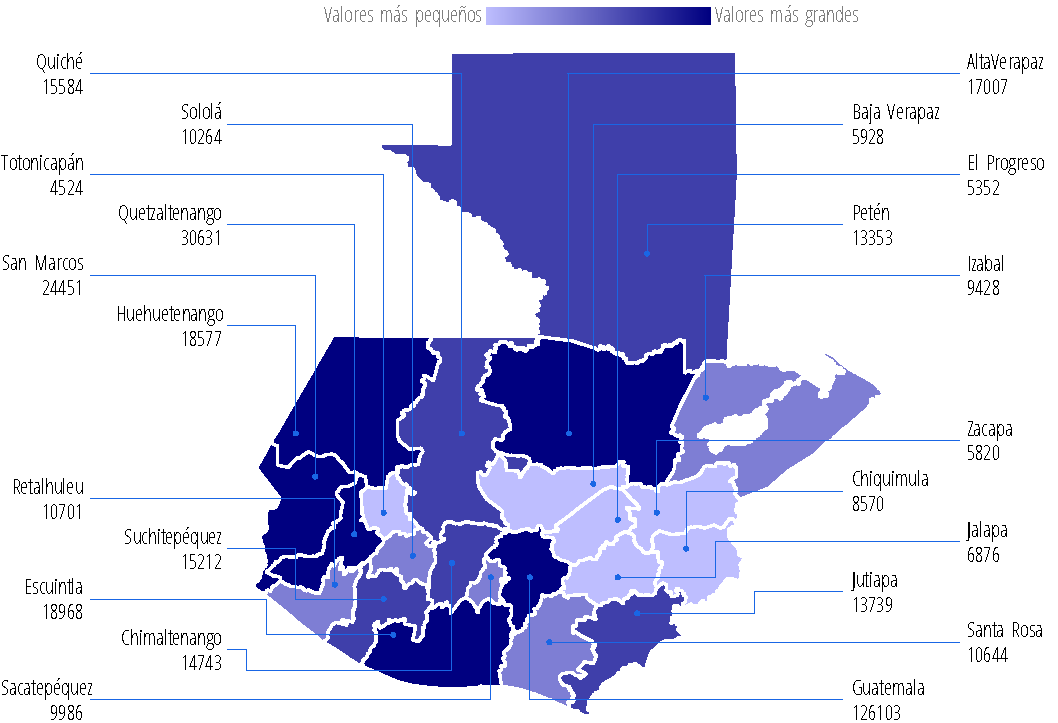
\includegraphics[width=52\cuadri]{graficas/diversificado/1_7.pdf} }{Instituto Nacional de Estadística, con datos del Ministerio de Educación}




\INEchaptercarta[Indicadores de educación diversificada]{Indicadores\\ de educación diversificada}{}


\cajita{Cobertura bruta}{La tasa bruta de cobertura en diversificado establece una relación entre la inscripción inicial total sin distinción de edad.
	
	En el año 2009 fue de 33.4\% en el año 2014 fue de 38.0\%, lo cual fue un aumento de 4.7 puntos porcentuales.}{Tasa bruta de cobertura del ciclo de educación diversificada}{República de Guatemala, serie histórica, en porcentaje}{\ \\[0mm]\begin{tikzpicture}[x=1pt,y=1pt]  % Created by tikzDevice version 0.10.1 on 2016-02-29 12:47:20
% !TEX encoding = UTF-8 Unicode
\definecolor{fillColor}{RGB}{255,255,255}
\path[use as bounding box,fill=fillColor,fill opacity=0.00] (0,0) rectangle (289.08,198.74);
\begin{scope}
\path[clip] (  0.00,  0.00) rectangle (289.08,198.74);

\path[] (  0.00,  0.00) rectangle (289.08,198.74);
\end{scope}
\begin{scope}
\path[clip] (  0.00,  0.00) rectangle (289.08,198.74);

\path[] ( -0.52, 15.61) rectangle (280.54,191.48);

\path[] (  0.00, 35.12) --
	(280.54, 35.12);

\path[] (  0.00, 81.16) --
	(280.54, 81.16);

\path[] (  0.00,127.20) --
	(280.54,127.20);

\path[] (  0.00,173.24) --
	(280.54,173.24);

\path[] (  0.00, 58.14) --
	(280.54, 58.14);

\path[] (  0.00,104.18) --
	(280.54,104.18);

\path[] (  0.00,150.22) --
	(280.54,150.22);

\path[] ( 26.68, 15.61) --
	( 26.68,191.48);

\path[] ( 72.01, 15.61) --
	( 72.01,191.48);

\path[] (117.35, 15.61) --
	(117.35,191.48);

\path[] (162.68, 15.61) --
	(162.68,191.48);

\path[] (208.01, 15.61) --
	(208.01,191.48);

\path[] (253.34, 15.61) --
	(253.34,191.48);
\definecolor{drawColor}{RGB}{0,0,255}

\path[draw=drawColor,line width= 1.7pt,line join=round] ( 26.68,119.95) --
	( 72.01,158.40) --
	(117.35,172.44) --
	(162.68,183.49) --
	(208.01,180.96) --
	(253.34,173.47);
\definecolor{drawColor}{RGB}{0,0,0}

\node[text=drawColor,anchor=base,inner sep=0pt, outer sep=0pt, scale=  1.02] at ( 26.68,108.04) {33.4};

\node[text=drawColor,anchor=base east,inner sep=0pt, outer sep=0pt, scale=  1.02] at ( 68.89,158.40) {36.7};

\node[text=drawColor,anchor=base east,inner sep=0pt, outer sep=0pt, scale=  1.02] at (114.22,172.44) {37.9};

\node[text=drawColor,anchor=base,inner sep=0pt, outer sep=0pt, scale=  1.02] at (162.68,187.46) {38.9};

\node[text=drawColor,anchor=base west,inner sep=0pt, outer sep=0pt, scale=  1.02] at (208.01,184.93) {38.7};

\node[text=drawColor,anchor=base,inner sep=0pt, outer sep=0pt, scale=  1.02] at (253.34,161.56) {38.0};

\path[draw=drawColor,line width= 0.1pt,line join=round] (  0.00, 23.61) -- (280.54, 23.61);

\path[] ( -0.52, 15.61) rectangle (280.54,191.48);
\end{scope}
\begin{scope}
\path[clip] (  0.00,  0.00) rectangle (289.08,198.74);

\path[] (  0.00, 15.61) --
	(280.54, 15.61);
\end{scope}
\begin{scope}
\path[clip] (  0.00,  0.00) rectangle (289.08,198.74);

\path[] ( 26.68, 12.86) --
	( 26.68, 15.61);

\path[] ( 72.01, 12.86) --
	( 72.01, 15.61);

\path[] (117.35, 12.86) --
	(117.35, 15.61);

\path[] (162.68, 12.86) --
	(162.68, 15.61);

\path[] (208.01, 12.86) --
	(208.01, 15.61);

\path[] (253.34, 12.86) --
	(253.34, 15.61);
\end{scope}
\begin{scope}
\path[clip] (  0.00,  0.00) rectangle (289.08,198.74);
\definecolor{drawColor}{RGB}{0,0,0}

\node[text=drawColor,anchor=base,inner sep=0pt, outer sep=0pt, scale=  1.00] at ( 26.68,  2.85) {2009};

\node[text=drawColor,anchor=base,inner sep=0pt, outer sep=0pt, scale=  1.00] at ( 72.01,  2.85) {2010};

\node[text=drawColor,anchor=base,inner sep=0pt, outer sep=0pt, scale=  1.00] at (117.35,  2.85) {2011};

\node[text=drawColor,anchor=base,inner sep=0pt, outer sep=0pt, scale=  1.00] at (162.68,  2.85) {2012};

\node[text=drawColor,anchor=base,inner sep=0pt, outer sep=0pt, scale=  1.00] at (208.01,  2.85) {2013};

\node[text=drawColor,anchor=base,inner sep=0pt, outer sep=0pt, scale=  1.00] at (253.34,  2.85) {2014};
\end{scope}
  \end{tikzpicture}}{Instituto Nacional de Estadística, con datos del Ministerio de Educación}

\cajita{Cobertura bruta por sexo}{La tasa bruta de cobertura en diversificado por sexo fue del 37.7\% para hombres y 38.3\% para mujeres.}{Tasa bruta de cobertura del ciclo de educación diversificada, por sexo}{República de Guatemala, año 2014, en porcentaje}{\ \\[0mm]\begin{tikzpicture}[x=1pt,y=1pt]  % Created by tikzDevice version 0.7.0 on 2015-08-28 13:12:27
% !TEX encoding = UTF-8 Unicode
\definecolor[named]{fillColor}{rgb}{1.00,1.00,1.00}
\path[use as bounding box,fill=fillColor,fill opacity=0.00] (0,0) rectangle (289.08,198.74);
\begin{scope}
\path[clip] (  0.00,  0.00) rectangle (289.08,198.74);
\definecolor[named]{drawColor}{rgb}{1.00,1.00,1.00}

\path[draw=drawColor,line width= 0.6pt,line join=round,line cap=round] (  0.00,  0.00) rectangle (289.08,198.74);
\end{scope}
\begin{scope}
\path[clip] (  0.00,  0.00) rectangle (289.08,198.74);

\path[] (  7.11, 23.47) rectangle (289.08,181.67);

\path[] ( 59.98, 23.47) --
	( 59.98,181.67);

\path[] (148.10, 23.47) --
	(148.10,181.67);

\path[] (236.21, 23.47) --
	(236.21,181.67);
\definecolor[named]{drawColor}{rgb}{0.00,0.00,1.00}
\definecolor[named]{fillColor}{rgb}{0.00,0.00,1.00}

\path[draw=drawColor,line width= 0.6pt,line join=round,fill=fillColor] ( 40.16, 23.47) rectangle ( 79.81,181.26);

\path[draw=drawColor,line width= 0.6pt,line join=round,fill=fillColor] (128.27, 23.47) rectangle (167.92,180.86);

\path[draw=drawColor,line width= 0.6pt,line join=round,fill=fillColor] (216.39, 23.47) rectangle (256.04,181.67);
\definecolor[named]{drawColor}{rgb}{0.00,0.00,0.00}
\definecolor[named]{fillColor}{rgb}{0.00,0.00,0.00}

\path[draw=drawColor,line width= 0.1pt,line join=round,fill=fillColor] (  7.11, 23.47) -- (289.08, 23.47);

\node[text=drawColor,anchor=base,inner sep=0pt, outer sep=0pt, scale=  1.01] at ( 59.98,185.22) {38.7};

\node[text=drawColor,anchor=base,inner sep=0pt, outer sep=0pt, scale=  1.01] at (148.10,184.81) {38.6};

\node[text=drawColor,anchor=base,inner sep=0pt, outer sep=0pt, scale=  1.01] at (236.21,185.63) {38.8};
\end{scope}
\begin{scope}
\path[clip] (  0.00,  0.00) rectangle (289.08,198.74);

\path[] (  7.11, 23.47) --
	(  7.11,181.67);
\end{scope}
\begin{scope}
\path[clip] (  0.00,  0.00) rectangle (289.08,198.74);

\path[] (  7.11, 23.47) --
	(289.08, 23.47);
\end{scope}
\begin{scope}
\path[clip] (  0.00,  0.00) rectangle (289.08,198.74);

\path[] ( 59.98, 19.20) --
	( 59.98, 23.47);

\path[] (148.10, 19.20) --
	(148.10, 23.47);

\path[] (236.21, 19.20) --
	(236.21, 23.47);
\end{scope}
\begin{scope}
\path[clip] (  0.00,  0.00) rectangle (289.08,198.74);
\definecolor[named]{drawColor}{rgb}{0.00,0.00,0.00}

\node[text=drawColor,anchor=base,inner sep=0pt, outer sep=0pt, scale=  1.00] at ( 59.98,  8.54) {Total};

\node[text=drawColor,anchor=base,inner sep=0pt, outer sep=0pt, scale=  1.00] at (148.10,  8.54) {Hombre};

\node[text=drawColor,anchor=base,inner sep=0pt, outer sep=0pt, scale=  1.00] at (236.21,  8.54) {Mujer};
\end{scope}
  \end{tikzpicture}}{Instituto Nacional de Estadística, con datos del Ministerio de Educación}

\cajota{Cobertura bruta en los departamentos}{Los departamentos con las menores tasas brutas de cobertura en diversificado en el 2014 fueron: Huehuetenango 21.6\%, Alta Verapaz 19.2\% y Totonicapán 15.0\%.
	
	 Los departamentos con las mayores tasas brutas de cobertura en diversificado: Guatemala 62.5\%, Quetzaltenango 57.0\% y  Retalhuleu 49.6\%.}{Tasa bruta de cobertura del ciclo de educación diversificada}{Por departamento, año 2014, en porcentaje}{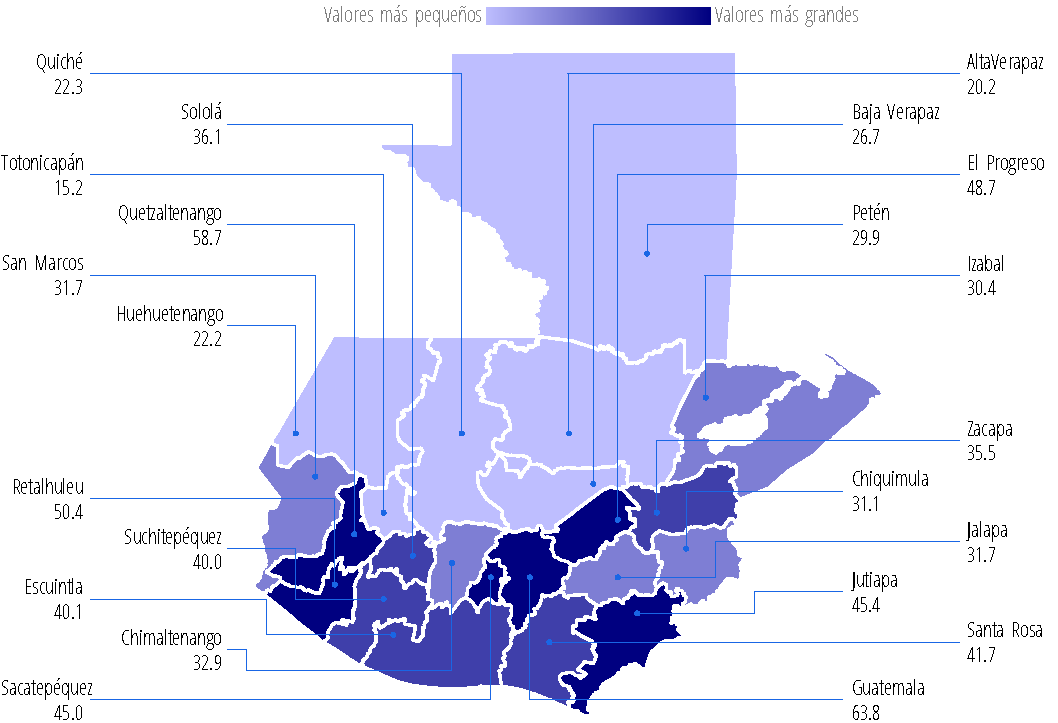
\includegraphics[width=52\cuadri]{graficas/diversificado/1_10.pdf} }{Instituto Nacional de Estadística, con datos del Ministerio de Educación}

\cajita{Cobertura neta}{La tasa neta de cobertura en diversificado es la relación que existe entre la parte de la inscripción inicial que se encuentra en la edad escolar de 16 a 19 años y la población en edad escolar de 16 a 19 años.
	
	En el año 2009 el 21.2\% de cobertura y en el 2014 fue de 24.4\% el cual fue un aumento en 3.2 puntos porcentuales.}{Tasa neta de cobertura del ciclo de educación diversificada}{República de Guatemala, serie histórica, en porcentaje}{\ \\[0mm]\begin{tikzpicture}[x=1pt,y=1pt]  % Created by tikzDevice version 0.10.1 on 2016-02-29 12:47:47
% !TEX encoding = UTF-8 Unicode
\definecolor{fillColor}{RGB}{255,255,255}
\path[use as bounding box,fill=fillColor,fill opacity=0.00] (0,0) rectangle (289.08,198.74);
\begin{scope}
\path[clip] (  0.00,  0.00) rectangle (289.08,198.74);

\path[] (  0.00,  0.00) rectangle (289.08,198.74);
\end{scope}
\begin{scope}
\path[clip] (  0.00,  0.00) rectangle (289.08,198.74);

\path[] ( -0.52, 15.61) rectangle (280.54,191.48);

\path[] (  0.00, 51.17) --
	(280.54, 51.17);

\path[] (  0.00,106.30) --
	(280.54,106.30);

\path[] (  0.00,161.44) --
	(280.54,161.44);

\path[] (  0.00, 23.61) --
	(280.54, 23.61);

\path[] (  0.00, 78.74) --
	(280.54, 78.74);

\path[] (  0.00,133.87) --
	(280.54,133.87);

\path[] (  0.00,189.00) --
	(280.54,189.00);

\path[] ( 26.68, 15.61) --
	( 26.68,191.48);

\path[] ( 72.01, 15.61) --
	( 72.01,191.48);

\path[] (117.35, 15.61) --
	(117.35,191.48);

\path[] (162.68, 15.61) --
	(162.68,191.48);

\path[] (208.01, 15.61) --
	(208.01,191.48);

\path[] (253.34, 15.61) --
	(253.34,191.48);
\definecolor{drawColor}{RGB}{0,0,255}

\path[draw=drawColor,line width= 1.7pt,line join=round] ( 26.68,147.21) --
	( 72.01,159.56) --
	(117.35,172.35) --
	(162.68,179.74) --
	(208.01,183.49) --
	(253.34,182.17);
\definecolor{drawColor}{RGB}{0,0,0}

\node[text=drawColor,anchor=base,inner sep=0pt, outer sep=0pt, scale=  1.02] at ( 26.68,135.30) {21.2};

\node[text=drawColor,anchor=base east,inner sep=0pt, outer sep=0pt, scale=  1.02] at ( 68.89,159.56) {22.3};

\node[text=drawColor,anchor=base east,inner sep=0pt, outer sep=0pt, scale=  1.02] at (114.22,172.35) {23.5};

\node[text=drawColor,anchor=base east,inner sep=0pt, outer sep=0pt, scale=  1.02] at (159.55,179.74) {24.2};

\node[text=drawColor,anchor=base,inner sep=0pt, outer sep=0pt, scale=  1.02] at (208.01,187.46) {24.5};

\node[text=drawColor,anchor=base,inner sep=0pt, outer sep=0pt, scale=  1.02] at (253.34,170.25) {24.4};

\path[draw=drawColor,line width= 0.1pt,line join=round] (  0.00, 23.61) -- (280.54, 23.61);

\path[] ( -0.52, 15.61) rectangle (280.54,191.48);
\end{scope}
\begin{scope}
\path[clip] (  0.00,  0.00) rectangle (289.08,198.74);

\path[] (  0.00, 15.61) --
	(280.54, 15.61);
\end{scope}
\begin{scope}
\path[clip] (  0.00,  0.00) rectangle (289.08,198.74);

\path[] ( 26.68, 12.86) --
	( 26.68, 15.61);

\path[] ( 72.01, 12.86) --
	( 72.01, 15.61);

\path[] (117.35, 12.86) --
	(117.35, 15.61);

\path[] (162.68, 12.86) --
	(162.68, 15.61);

\path[] (208.01, 12.86) --
	(208.01, 15.61);

\path[] (253.34, 12.86) --
	(253.34, 15.61);
\end{scope}
\begin{scope}
\path[clip] (  0.00,  0.00) rectangle (289.08,198.74);
\definecolor{drawColor}{RGB}{0,0,0}

\node[text=drawColor,anchor=base,inner sep=0pt, outer sep=0pt, scale=  1.00] at ( 26.68,  2.85) {2009};

\node[text=drawColor,anchor=base,inner sep=0pt, outer sep=0pt, scale=  1.00] at ( 72.01,  2.85) {2010};

\node[text=drawColor,anchor=base,inner sep=0pt, outer sep=0pt, scale=  1.00] at (117.35,  2.85) {2011};

\node[text=drawColor,anchor=base,inner sep=0pt, outer sep=0pt, scale=  1.00] at (162.68,  2.85) {2012};

\node[text=drawColor,anchor=base,inner sep=0pt, outer sep=0pt, scale=  1.00] at (208.01,  2.85) {2013};

\node[text=drawColor,anchor=base,inner sep=0pt, outer sep=0pt, scale=  1.00] at (253.34,  2.85) {2014};
\end{scope}
  \end{tikzpicture}}{Instituto Nacional de Estadística, con datos del Ministerio de Educación}

\cajita{Cobertura neta por sexo}{La tasa neta de cobertura en diversificado por sexo fue del 23.8\% para hombres y 24.9\% para las mujeres.}{Tasa neta de cobertura del ciclo de educación diversificada, por sexo}{República de Guatemala, año 2014, en porcentaje}{\ \\[0mm]\begin{tikzpicture}[x=1pt,y=1pt]  % Created by tikzDevice version 0.10.1 on 2016-02-29 12:48:12
% !TEX encoding = UTF-8 Unicode
\definecolor{fillColor}{RGB}{255,255,255}
\path[use as bounding box,fill=fillColor,fill opacity=0.00] (0,0) rectangle (289.08,198.74);
\begin{scope}
\path[clip] (  0.00,  0.00) rectangle (289.08,198.74);

\path[] (  0.00,  0.00) rectangle (289.08,198.74);
\end{scope}
\begin{scope}
\path[clip] (  0.00,  0.00) rectangle (289.08,198.74);

\path[] (  0.00, 12.77) rectangle (289.08,181.67);

\path[] ( 54.20, 12.77) --
	( 54.20,181.67);

\path[] (144.54, 12.77) --
	(144.54,181.67);

\path[] (234.88, 12.77) --
	(234.88,181.67);
\definecolor{drawColor}{RGB}{0,0,255}
\definecolor{fillColor}{RGB}{0,0,255}

\path[draw=drawColor,line width= 0.6pt,line join=round,fill=fillColor] ( 36.13, 20.44) rectangle ( 72.27,170.67);

\path[draw=drawColor,line width= 0.6pt,line join=round,fill=fillColor] (126.47, 20.44) rectangle (162.61,167.34);

\path[draw=drawColor,line width= 0.6pt,line join=round,fill=fillColor] (216.81, 20.44) rectangle (252.95,173.99);
\definecolor{drawColor}{RGB}{0,0,0}

\path[draw=drawColor,line width= 0.1pt,line join=round] (  0.00, 20.44) -- (289.08, 20.44);

\node[text=drawColor,anchor=base,inner sep=0pt, outer sep=0pt, scale=  1.02] at ( 54.20,174.64) {24.4};

\node[text=drawColor,anchor=base,inner sep=0pt, outer sep=0pt, scale=  1.02] at (144.54,171.31) {23.8};

\node[text=drawColor,anchor=base,inner sep=0pt, outer sep=0pt, scale=  1.02] at (234.88,177.96) {24.9};

\path[] (  0.00, 12.77) rectangle (289.08,181.67);
\end{scope}
\begin{scope}
\path[clip] (  0.00,  0.00) rectangle (289.08,198.74);

\path[] (  0.00, 12.77) --
	(289.08, 12.77);
\end{scope}
\begin{scope}
\path[clip] (  0.00,  0.00) rectangle (289.08,198.74);

\path[] ( 54.20, 10.02) --
	( 54.20, 12.77);

\path[] (144.54, 10.02) --
	(144.54, 12.77);

\path[] (234.88, 10.02) --
	(234.88, 12.77);
\end{scope}
\begin{scope}
\path[clip] (  0.00,  0.00) rectangle (289.08,198.74);
\definecolor{drawColor}{RGB}{0,0,0}

\node[text=drawColor,anchor=base,inner sep=0pt, outer sep=0pt, scale=  1.00] at ( 54.20, -0.00) {Total};

\node[text=drawColor,anchor=base,inner sep=0pt, outer sep=0pt, scale=  1.00] at (144.54, -0.00) {Hombre};

\node[text=drawColor,anchor=base,inner sep=0pt, outer sep=0pt, scale=  1.00] at (234.88, -0.00) {Mujer};
\end{scope}
  \end{tikzpicture}}{Instituto Nacional de Estadística, con datos del Ministerio de Educación}

\cajota{Cobertura neta en los departamentos}{Los departamentos con las menores tasas netas de cobertura en diversificado en el 2014 fueron: Quiché 12.4\%, Alta Verapaz 10.3\% y Totonicapán 9.2\%.

	 Los departamentos con las más altas tasas netas de cobertura en diversificado fueron:  Guatemala 41.3\%, Quetzaltenango 36.5\% y El Progreso 33.3\%. }{Tasa neta de cobertura del ciclo de educación diversificada}{Por departamento, año 2014, en porcentaje}{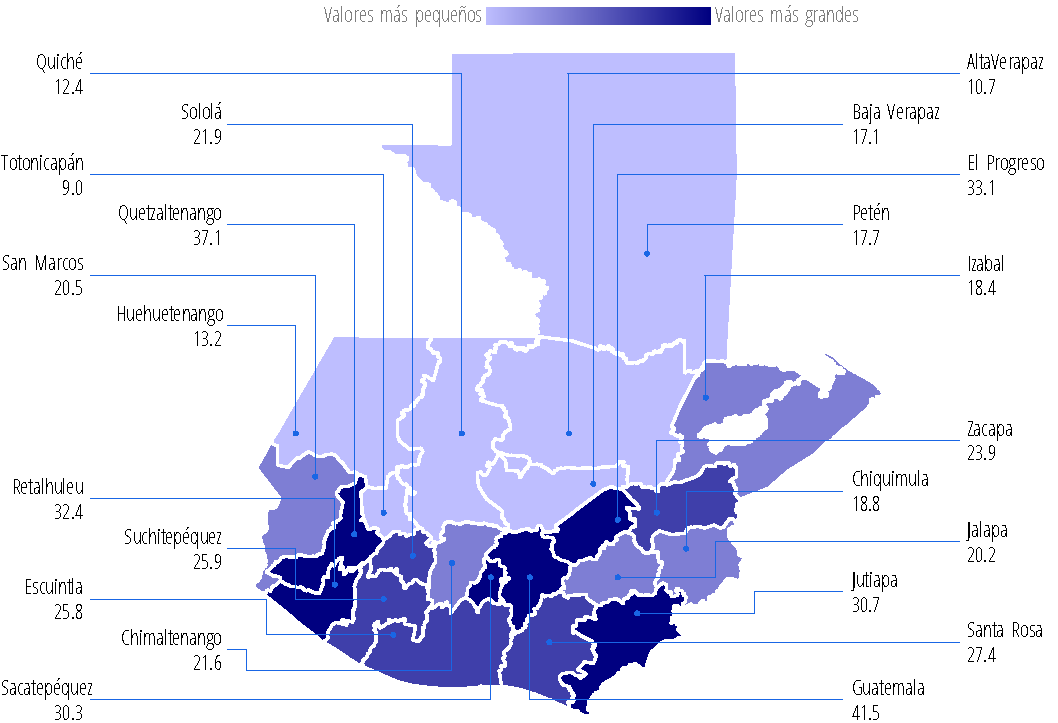
\includegraphics[width=52\cuadri]{graficas/diversificado/1_13.pdf} }{Instituto Nacional de Estadística, con datos del Ministerio de Educación}




\cajita{Repitencia}{La tasa de repitencia en diversificado es la relación que existe entre el número de repitentes y el número de alumnos que en el año  estaban inscritos en el mismo grado.
	
	En el año 2009 fue  del 1.2\% y en el año 2014 fue de 0.8\% lo cual representó una disminución en 0.4 puntos porcentuales.}{Tasa de repitencia del ciclo de educación diversificada}{República de Guatemala, serie histórica, en porcentaje}{\ \\[0mm]\begin{tikzpicture}[x=1pt,y=1pt]  % Created by tikzDevice version 0.10.1 on 2016-02-29 12:48:20
% !TEX encoding = UTF-8 Unicode
\definecolor{fillColor}{RGB}{255,255,255}
\path[use as bounding box,fill=fillColor,fill opacity=0.00] (0,0) rectangle (289.08,198.74);
\begin{scope}
\path[clip] (  0.00,  0.00) rectangle (289.08,198.74);

\path[] (  0.00,  0.00) rectangle (289.08,198.74);
\end{scope}
\begin{scope}
\path[clip] (  0.00,  0.00) rectangle (289.08,198.74);

\path[] ( 10.27, 15.61) rectangle (280.54,191.48);

\path[] ( 10.27, 47.68) --
	(280.54, 47.68);

\path[] ( 10.27, 95.84) --
	(280.54, 95.84);

\path[] ( 10.27,144.00) --
	(280.54,144.00);

\path[] ( 10.27, 23.61) --
	(280.54, 23.61);

\path[] ( 10.27, 71.76) --
	(280.54, 71.76);

\path[] ( 10.27,119.92) --
	(280.54,119.92);

\path[] ( 10.27,168.08) --
	(280.54,168.08);

\path[] ( 36.43, 15.61) --
	( 36.43,191.48);

\path[] ( 80.02, 15.61) --
	( 80.02,191.48);

\path[] (123.61, 15.61) --
	(123.61,191.48);

\path[] (167.20, 15.61) --
	(167.20,191.48);

\path[] (210.80, 15.61) --
	(210.80,191.48);

\path[] (254.39, 15.61) --
	(254.39,191.48);
\definecolor{drawColor}{RGB}{0,0,255}

\path[draw=drawColor,line width= 1.7pt,line join=round] ( 36.43,135.33) --
	( 80.02,111.25) --
	(123.61,101.62) --
	(167.20,183.49) --
	(210.80,114.14) --
	(254.39, 98.73);
\definecolor{drawColor}{RGB}{0,0,0}

\node[text=drawColor,anchor=base,inner sep=0pt, outer sep=0pt, scale=  1.02] at ( 36.43,139.30) {1.2};

\node[text=drawColor,anchor=base west,inner sep=0pt, outer sep=0pt, scale=  1.02] at ( 80.02,115.22) {0.9};

\node[text=drawColor,anchor=base,inner sep=0pt, outer sep=0pt, scale=  1.02] at (123.61, 89.71) {0.8};

\node[text=drawColor,anchor=base,inner sep=0pt, outer sep=0pt, scale=  1.02] at (167.20,187.46) {1.7};

\node[text=drawColor,anchor=base west,inner sep=0pt, outer sep=0pt, scale=  1.02] at (210.80,118.11) {0.9};

\node[text=drawColor,anchor=base,inner sep=0pt, outer sep=0pt, scale=  1.02] at (254.39, 86.82) {0.8};

\path[draw=drawColor,line width= 0.1pt,line join=round] ( 10.27, 23.61) -- (280.54, 23.61);

\path[] ( 10.27, 15.61) rectangle (280.54,191.48);
\end{scope}
\begin{scope}
\path[clip] (  0.00,  0.00) rectangle (289.08,198.74);

\path[] ( 10.27, 15.61) --
	( 10.27,191.48);
\end{scope}
\begin{scope}
\path[clip] (  0.00,  0.00) rectangle (289.08,198.74);
\definecolor{drawColor}{RGB}{255,255,255}

\node[text=drawColor,text opacity=0.00,anchor=base east,inner sep=0pt, outer sep=0pt, scale=  1.00] at (  5.32, 19.70) {0.0};

\node[text=drawColor,text opacity=0.00,anchor=base east,inner sep=0pt, outer sep=0pt, scale=  1.00] at (  5.32, 67.86) {0.5};

\node[text=drawColor,text opacity=0.00,anchor=base east,inner sep=0pt, outer sep=0pt, scale=  1.00] at (  5.32,116.01) {1.0};

\node[text=drawColor,text opacity=0.00,anchor=base east,inner sep=0pt, outer sep=0pt, scale=  1.00] at (  5.32,164.17) {1.5};
\end{scope}
\begin{scope}
\path[clip] (  0.00,  0.00) rectangle (289.08,198.74);

\path[] (  7.52, 23.61) --
	( 10.27, 23.61);

\path[] (  7.52, 71.76) --
	( 10.27, 71.76);

\path[] (  7.52,119.92) --
	( 10.27,119.92);

\path[] (  7.52,168.08) --
	( 10.27,168.08);
\end{scope}
\begin{scope}
\path[clip] (  0.00,  0.00) rectangle (289.08,198.74);

\path[] ( 10.27, 15.61) --
	(280.54, 15.61);
\end{scope}
\begin{scope}
\path[clip] (  0.00,  0.00) rectangle (289.08,198.74);

\path[] ( 36.43, 12.86) --
	( 36.43, 15.61);

\path[] ( 80.02, 12.86) --
	( 80.02, 15.61);

\path[] (123.61, 12.86) --
	(123.61, 15.61);

\path[] (167.20, 12.86) --
	(167.20, 15.61);

\path[] (210.80, 12.86) --
	(210.80, 15.61);

\path[] (254.39, 12.86) --
	(254.39, 15.61);
\end{scope}
\begin{scope}
\path[clip] (  0.00,  0.00) rectangle (289.08,198.74);
\definecolor{drawColor}{RGB}{0,0,0}

\node[text=drawColor,anchor=base,inner sep=0pt, outer sep=0pt, scale=  1.00] at ( 36.43,  2.85) {2009};

\node[text=drawColor,anchor=base,inner sep=0pt, outer sep=0pt, scale=  1.00] at ( 80.02,  2.85) {2010};

\node[text=drawColor,anchor=base,inner sep=0pt, outer sep=0pt, scale=  1.00] at (123.61,  2.85) {2011};

\node[text=drawColor,anchor=base,inner sep=0pt, outer sep=0pt, scale=  1.00] at (167.20,  2.85) {2012};

\node[text=drawColor,anchor=base,inner sep=0pt, outer sep=0pt, scale=  1.00] at (210.80,  2.85) {2013};

\node[text=drawColor,anchor=base,inner sep=0pt, outer sep=0pt, scale=  1.00] at (254.39,  2.85) {2014};
\end{scope}
  \end{tikzpicture}}{Instituto Nacional de Estadística, con datos del Ministerio de Educación}

\cajita{Repitencia por sexo}{La tasa de repitencia en diversificado por sexo fue del 0.9\% para hombres y 0.7\% para las mujeres. }{Tasa de repitencia del ciclo de educación diversificada, por sexo}{República de Guatemala, año 2014, en porcentaje}{\ \\[0mm]\begin{tikzpicture}[x=1pt,y=1pt]  % Created by tikzDevice version 0.7.0 on 2015-08-28 13:12:27
% !TEX encoding = UTF-8 Unicode
\definecolor[named]{fillColor}{rgb}{1.00,1.00,1.00}
\path[use as bounding box,fill=fillColor,fill opacity=0.00] (0,0) rectangle (289.08,198.74);
\begin{scope}
\path[clip] (  0.00,  0.00) rectangle (289.08,198.74);
\definecolor[named]{drawColor}{rgb}{1.00,1.00,1.00}

\path[draw=drawColor,line width= 0.6pt,line join=round,line cap=round] (  0.00,  0.00) rectangle (289.08,198.74);
\end{scope}
\begin{scope}
\path[clip] (  0.00,  0.00) rectangle (289.08,198.74);

\path[] (  7.11, 23.47) rectangle (289.08,181.67);

\path[] ( 59.98, 23.47) --
	( 59.98,181.67);

\path[] (148.10, 23.47) --
	(148.10,181.67);

\path[] (236.21, 23.47) --
	(236.21,181.67);
\definecolor[named]{drawColor}{rgb}{0.00,0.00,1.00}
\definecolor[named]{fillColor}{rgb}{0.00,0.00,1.00}

\path[draw=drawColor,line width= 0.6pt,line join=round,fill=fillColor] ( 40.16, 23.47) rectangle ( 79.81,152.91);

\path[draw=drawColor,line width= 0.6pt,line join=round,fill=fillColor] (128.27, 23.47) rectangle (167.92,181.67);

\path[draw=drawColor,line width= 0.6pt,line join=round,fill=fillColor] (216.39, 23.47) rectangle (256.04,138.52);
\definecolor[named]{drawColor}{rgb}{0.00,0.00,0.00}
\definecolor[named]{fillColor}{rgb}{0.00,0.00,0.00}

\path[draw=drawColor,line width= 0.1pt,line join=round,fill=fillColor] (  7.11, 23.47) -- (289.08, 23.47);

\node[text=drawColor,anchor=base,inner sep=0pt, outer sep=0pt, scale=  1.01] at ( 59.98,156.86) {0.9};

\node[text=drawColor,anchor=base,inner sep=0pt, outer sep=0pt, scale=  1.01] at (148.10,185.63) {1.1};

\node[text=drawColor,anchor=base,inner sep=0pt, outer sep=0pt, scale=  1.01] at (236.21,142.48) {0.8};
\end{scope}
\begin{scope}
\path[clip] (  0.00,  0.00) rectangle (289.08,198.74);

\path[] (  7.11, 23.47) --
	(  7.11,181.67);
\end{scope}
\begin{scope}
\path[clip] (  0.00,  0.00) rectangle (289.08,198.74);

\path[] (  7.11, 23.47) --
	(289.08, 23.47);
\end{scope}
\begin{scope}
\path[clip] (  0.00,  0.00) rectangle (289.08,198.74);

\path[] ( 59.98, 19.20) --
	( 59.98, 23.47);

\path[] (148.10, 19.20) --
	(148.10, 23.47);

\path[] (236.21, 19.20) --
	(236.21, 23.47);
\end{scope}
\begin{scope}
\path[clip] (  0.00,  0.00) rectangle (289.08,198.74);
\definecolor[named]{drawColor}{rgb}{0.00,0.00,0.00}

\node[text=drawColor,anchor=base,inner sep=0pt, outer sep=0pt, scale=  1.00] at ( 59.98,  8.54) {Total};

\node[text=drawColor,anchor=base,inner sep=0pt, outer sep=0pt, scale=  1.00] at (148.10,  8.54) {Hombre};

\node[text=drawColor,anchor=base,inner sep=0pt, outer sep=0pt, scale=  1.00] at (236.21,  8.54) {Mujer};
\end{scope}
  \end{tikzpicture}}{Instituto Nacional de Estadística, con datos del Ministerio de Educación}

\cajota{Repitencia en los departamentos}{El mapa muestra en color celeste los departamentos con las menores tasas de repitencia en diversificado fueron: Suchitepéquez 0.3\%, Jutiapa 0.3\%  y Petén 0.2\%.
	
	 Los departamentos con las más  altas tasa de repitencia en diversificado en el 2014 fueron: Zacapa 1.4\%, Alta Verapaz 1.2\% y Totonicapán 1.2\%. El departamento de Guatemala presentó una tasa de repitencia de 1.0\%.}{Tasa de repitencia del ciclo de educación diversificada}{Por departamento, año 2014, en porcentaje}{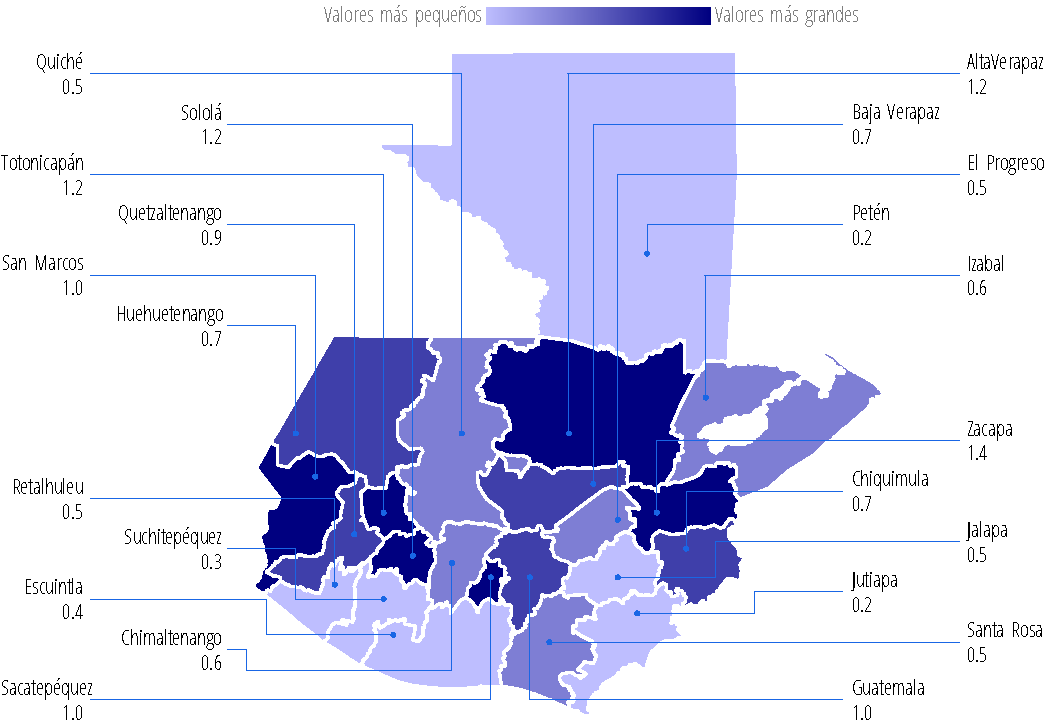
\includegraphics[width=52\cuadri]{graficas/diversificado/1_16.pdf} }{Instituto Nacional de Estadística, con datos del Ministerio de Educación}






\cajita{Sobre-edad}{La tasa de sobre-edad en diversificado es la relación que existe entre la cantidad de alumnos inscritos en los diferentes grados de un nivel educativo, con dos o más años de atraso escolar por encima de la edad correspondiente al grado de estudio.
	
	En el año 2009 fue de 31.3\% y en el 2014 fue 26.6\%, una disminución en 4.7 puntos porcentuales.}{Tasa de sobre-edad del ciclo de educación diversificada}{República de Guatemala, serie histórica, en porcentaje}{\ \\[0mm]\begin{tikzpicture}[x=1pt,y=1pt]  % Created by tikzDevice version 0.10.1 on 2016-02-29 12:48:35
% !TEX encoding = UTF-8 Unicode
\definecolor{fillColor}{RGB}{255,255,255}
\path[use as bounding box,fill=fillColor,fill opacity=0.00] (0,0) rectangle (289.08,198.74);
\begin{scope}
\path[clip] (  0.00,  0.00) rectangle (289.08,198.74);

\path[] (  0.00,  0.00) rectangle (289.08,198.74);
\end{scope}
\begin{scope}
\path[clip] (  0.00,  0.00) rectangle (289.08,198.74);

\path[] (  6.12, 15.61) rectangle (280.54,191.48);

\path[] (  6.12, 41.28) --
	(280.54, 41.28);

\path[] (  6.12, 76.62) --
	(280.54, 76.62);

\path[] (  6.12,111.96) --
	(280.54,111.96);

\path[] (  6.12,147.30) --
	(280.54,147.30);

\path[] (  6.12,182.64) --
	(280.54,182.64);

\path[] (  6.12, 23.61) --
	(280.54, 23.61);

\path[] (  6.12, 58.95) --
	(280.54, 58.95);

\path[] (  6.12, 94.29) --
	(280.54, 94.29);

\path[] (  6.12,129.63) --
	(280.54,129.63);

\path[] (  6.12,164.97) --
	(280.54,164.97);

\path[] ( 32.67, 15.61) --
	( 32.67,191.48);

\path[] ( 76.94, 15.61) --
	( 76.94,191.48);

\path[] (121.20, 15.61) --
	(121.20,191.48);

\path[] (165.46, 15.61) --
	(165.46,191.48);

\path[] (209.72, 15.61) --
	(209.72,191.48);

\path[] (253.99, 15.61) --
	(253.99,191.48);
\definecolor{drawColor}{RGB}{0,0,255}

\path[draw=drawColor,line width= 1.7pt,line join=round] ( 32.67,183.49) --
	( 76.94,171.90) --
	(121.20,162.71) --
	(165.46,162.99) --
	(209.72,142.63) --
	(253.99,117.19);
\definecolor{drawColor}{RGB}{0,0,0}

\node[text=drawColor,anchor=base,inner sep=0pt, outer sep=0pt, scale=  1.02] at ( 32.67,187.46) {31.3};

\node[text=drawColor,anchor=base west,inner sep=0pt, outer sep=0pt, scale=  1.02] at ( 76.94,175.87) {30.5};

\node[text=drawColor,anchor=base,inner sep=0pt, outer sep=0pt, scale=  1.02] at (121.20,150.80) {29.8};

\node[text=drawColor,anchor=base,inner sep=0pt, outer sep=0pt, scale=  1.02] at (165.46,166.96) {29.9};

\node[text=drawColor,anchor=base west,inner sep=0pt, outer sep=0pt, scale=  1.02] at (209.72,146.61) {28.4};

\node[text=drawColor,anchor=base,inner sep=0pt, outer sep=0pt, scale=  1.02] at (253.99,105.28) {26.6};

\path[draw=drawColor,line width= 0.1pt,line join=round] (  6.12, 23.61) -- (280.54, 23.61);

\path[] (  6.12, 15.61) rectangle (280.54,191.48);
\end{scope}
\begin{scope}
\path[clip] (  0.00,  0.00) rectangle (289.08,198.74);

\path[] (  6.12, 15.61) --
	(  6.12,191.48);
\end{scope}
\begin{scope}
\path[clip] (  0.00,  0.00) rectangle (289.08,198.74);
\definecolor{drawColor}{RGB}{255,255,255}

\node[text=drawColor,text opacity=0.00,anchor=base east,inner sep=0pt, outer sep=0pt, scale=  1.00] at (  1.17, 19.70) {20.0};

\node[text=drawColor,text opacity=0.00,anchor=base east,inner sep=0pt, outer sep=0pt, scale=  1.00] at (  1.17, 55.04) {22.5};

\node[text=drawColor,text opacity=0.00,anchor=base east,inner sep=0pt, outer sep=0pt, scale=  1.00] at (  1.17, 90.38) {25.0};

\node[text=drawColor,text opacity=0.00,anchor=base east,inner sep=0pt, outer sep=0pt, scale=  1.00] at (  1.17,125.72) {27.5};

\node[text=drawColor,text opacity=0.00,anchor=base east,inner sep=0pt, outer sep=0pt, scale=  1.00] at (  1.17,161.06) {30.0};
\end{scope}
\begin{scope}
\path[clip] (  0.00,  0.00) rectangle (289.08,198.74);

\path[] (  3.37, 23.61) --
	(  6.12, 23.61);

\path[] (  3.37, 58.95) --
	(  6.12, 58.95);

\path[] (  3.37, 94.29) --
	(  6.12, 94.29);

\path[] (  3.37,129.63) --
	(  6.12,129.63);

\path[] (  3.37,164.97) --
	(  6.12,164.97);
\end{scope}
\begin{scope}
\path[clip] (  0.00,  0.00) rectangle (289.08,198.74);

\path[] (  6.12, 15.61) --
	(280.54, 15.61);
\end{scope}
\begin{scope}
\path[clip] (  0.00,  0.00) rectangle (289.08,198.74);

\path[] ( 32.67, 12.86) --
	( 32.67, 15.61);

\path[] ( 76.94, 12.86) --
	( 76.94, 15.61);

\path[] (121.20, 12.86) --
	(121.20, 15.61);

\path[] (165.46, 12.86) --
	(165.46, 15.61);

\path[] (209.72, 12.86) --
	(209.72, 15.61);

\path[] (253.99, 12.86) --
	(253.99, 15.61);
\end{scope}
\begin{scope}
\path[clip] (  0.00,  0.00) rectangle (289.08,198.74);
\definecolor{drawColor}{RGB}{0,0,0}

\node[text=drawColor,anchor=base,inner sep=0pt, outer sep=0pt, scale=  1.00] at ( 32.67,  2.85) {2009};

\node[text=drawColor,anchor=base,inner sep=0pt, outer sep=0pt, scale=  1.00] at ( 76.94,  2.85) {2010};

\node[text=drawColor,anchor=base,inner sep=0pt, outer sep=0pt, scale=  1.00] at (121.20,  2.85) {2011};

\node[text=drawColor,anchor=base,inner sep=0pt, outer sep=0pt, scale=  1.00] at (165.46,  2.85) {2012};

\node[text=drawColor,anchor=base,inner sep=0pt, outer sep=0pt, scale=  1.00] at (209.72,  2.85) {2013};

\node[text=drawColor,anchor=base,inner sep=0pt, outer sep=0pt, scale=  1.00] at (253.99,  2.85) {2014};
\end{scope}
  \end{tikzpicture}}{Instituto Nacional de Estadística, con datos del Ministerio de Educación}

\cajita{Sobre-edad por sexo}{La tasa de sobre-edad en diversificado por sexo fue 28.9\% para hombres y 24.3\% para mujeres.}{Tasa de sobre-edad del ciclo de educación diversificada, por sexo}{República de Guatemala, año 2014, en porcentaje}{\ \\[0mm]\begin{tikzpicture}[x=1pt,y=1pt]  % Created by tikzDevice version 0.10.1 on 2016-02-29 12:49:04
% !TEX encoding = UTF-8 Unicode
\definecolor{fillColor}{RGB}{255,255,255}
\path[use as bounding box,fill=fillColor,fill opacity=0.00] (0,0) rectangle (289.08,198.74);
\begin{scope}
\path[clip] (  0.00,  0.00) rectangle (289.08,198.74);

\path[] (  0.00,  0.00) rectangle (289.08,198.74);
\end{scope}
\begin{scope}
\path[clip] (  0.00,  0.00) rectangle (289.08,198.74);

\path[] (  0.00, 12.77) rectangle (289.08,181.67);

\path[] ( 54.20, 12.77) --
	( 54.20,181.67);

\path[] (144.54, 12.77) --
	(144.54,181.67);

\path[] (234.88, 12.77) --
	(234.88,181.67);
\definecolor{drawColor}{RGB}{0,0,255}
\definecolor{fillColor}{RGB}{0,0,255}

\path[draw=drawColor,line width= 0.6pt,line join=round,fill=fillColor] ( 36.13, 20.44) rectangle ( 72.27,161.88);

\path[draw=drawColor,line width= 0.6pt,line join=round,fill=fillColor] (126.47, 20.44) rectangle (162.61,173.99);

\path[draw=drawColor,line width= 0.6pt,line join=round,fill=fillColor] (216.81, 20.44) rectangle (252.95,149.77);
\definecolor{drawColor}{RGB}{0,0,0}

\path[draw=drawColor,line width= 0.1pt,line join=round] (  0.00, 20.44) -- (289.08, 20.44);

\node[text=drawColor,anchor=base,inner sep=0pt, outer sep=0pt, scale=  1.02] at ( 54.20,165.85) {26.6};

\node[text=drawColor,anchor=base,inner sep=0pt, outer sep=0pt, scale=  1.02] at (144.54,177.96) {28.9};

\node[text=drawColor,anchor=base,inner sep=0pt, outer sep=0pt, scale=  1.02] at (234.88,153.74) {24.3};

\path[] (  0.00, 12.77) rectangle (289.08,181.67);
\end{scope}
\begin{scope}
\path[clip] (  0.00,  0.00) rectangle (289.08,198.74);

\path[] (  0.00, 12.77) --
	(289.08, 12.77);
\end{scope}
\begin{scope}
\path[clip] (  0.00,  0.00) rectangle (289.08,198.74);

\path[] ( 54.20, 10.02) --
	( 54.20, 12.77);

\path[] (144.54, 10.02) --
	(144.54, 12.77);

\path[] (234.88, 10.02) --
	(234.88, 12.77);
\end{scope}
\begin{scope}
\path[clip] (  0.00,  0.00) rectangle (289.08,198.74);
\definecolor{drawColor}{RGB}{0,0,0}

\node[text=drawColor,anchor=base,inner sep=0pt, outer sep=0pt, scale=  1.00] at ( 54.20, -0.00) {Total};

\node[text=drawColor,anchor=base,inner sep=0pt, outer sep=0pt, scale=  1.00] at (144.54, -0.00) {Hombre};

\node[text=drawColor,anchor=base,inner sep=0pt, outer sep=0pt, scale=  1.00] at (234.88, -0.00) {Mujer};
\end{scope}
  \end{tikzpicture}}{Instituto Nacional de Estadística, con datos del Ministerio de Educación}

\cajota{Sobre-edad en los departamentos}{El mapa muestra en color celeste los departamentos con las menores tasas de sobre-edad en diversificado: Quetzaltenango 22.2\%, El Progreso 21.5\% y Zacapa 19.6\%.
	
	 Los departamentos que en el 2014 tuvieron las más altas tasas  de sobre-edad en diversificado: Alta Verapaz 39.7\%, Quiché 35.2\% y Petén 30.4\%. En el departamento de Guatemala, la tasa de sobre-edad fue de 26.7\%. }{Tasa de sobre-edad del ciclo de educación diversificada}{Por departamento, año 2014, en porcentaje}{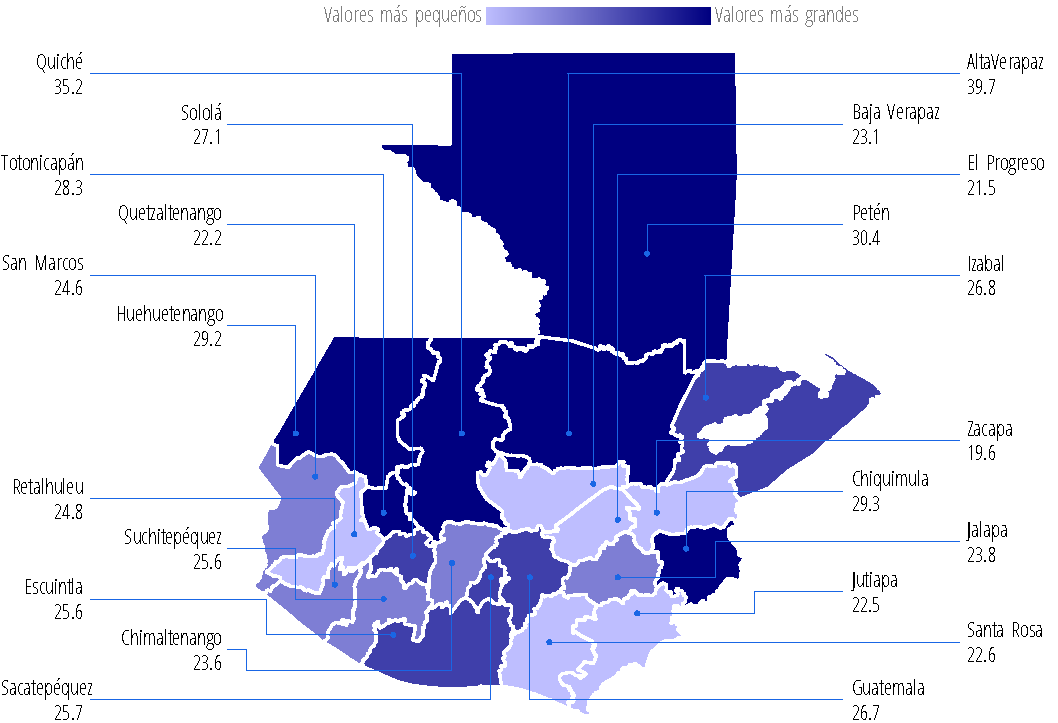
\includegraphics[width=52\cuadri]{graficas/diversificado/1_19.pdf} }{Instituto Nacional de Estadística, con datos del Ministerio de Educación}





\cajita{Deserción}{La tasa de deserción en diversificado se refiere a la cantidad de alumnos que no concluyen el ciclo lectivo.
	
	Presentó en el año 2009 el 6.5\% y en el año 2014 fue de 1.5\%, disminución en 5.0 puntos porcentuales.}{Tasa de deserción del ciclo de educación diversificada}{República de Guatemala, serie histórica, en porcentaje}{\ \\[0mm]\begin{tikzpicture}[x=1pt,y=1pt]  % Created by tikzDevice version 0.7.0 on 2015-08-31 18:35:32
% !TEX encoding = UTF-8 Unicode
\definecolor[named]{fillColor}{rgb}{1.00,1.00,1.00}
\path[use as bounding box,fill=fillColor,fill opacity=0.00] (0,0) rectangle (289.08,198.74);
\begin{scope}
\path[clip] (  0.00,  0.00) rectangle (289.08,198.74);
\definecolor[named]{drawColor}{rgb}{1.00,1.00,1.00}

\path[draw=drawColor,line width= 0.6pt,line join=round,line cap=round] (  0.00,  0.00) rectangle (289.08,198.74);
\end{scope}
\begin{scope}
\path[clip] (  0.00,  0.00) rectangle (289.08,198.74);

\path[] (  1.64, 17.78) rectangle (280.54,191.48);

\path[] (  1.64, 48.89) --
	(280.54, 48.89);

\path[] (  1.64, 95.34) --
	(280.54, 95.34);

\path[] (  1.64,141.79) --
	(280.54,141.79);

\path[] (  1.64,188.23) --
	(280.54,188.23);

\path[] (  1.64, 25.67) --
	(280.54, 25.67);

\path[] (  1.64, 72.12) --
	(280.54, 72.12);

\path[] (  1.64,118.56) --
	(280.54,118.56);

\path[] (  1.64,165.01) --
	(280.54,165.01);

\path[] ( 33.83, 17.78) --
	( 33.83,191.48);

\path[] ( 87.46, 17.78) --
	( 87.46,191.48);

\path[] (141.09, 17.78) --
	(141.09,191.48);

\path[] (194.73, 17.78) --
	(194.73,191.48);

\path[] (248.36, 17.78) --
	(248.36,191.48);
\definecolor[named]{drawColor}{rgb}{0.00,0.00,1.00}

\path[draw=drawColor,line width= 1.7pt,line join=round] ( 33.83,132.50) --
	( 87.46,183.59) --
	(141.09,114.85) --
	(194.73,103.70) --
	(248.36, 89.77);
\definecolor[named]{drawColor}{rgb}{0.00,0.00,0.00}

\node[text=drawColor,anchor=base,inner sep=0pt, outer sep=0pt, scale=  1.01] at ( 33.83,120.63) {6.5};

\node[text=drawColor,anchor=base,inner sep=0pt, outer sep=0pt, scale=  1.01] at ( 87.46,187.54) {12.0};

\node[text=drawColor,anchor=base west,inner sep=0pt, outer sep=0pt, scale=  1.01] at (141.09,118.80) {4.6};

\node[text=drawColor,anchor=base west,inner sep=0pt, outer sep=0pt, scale=  1.01] at (194.73,107.66) {3.4};

\node[text=drawColor,anchor=base,inner sep=0pt, outer sep=0pt, scale=  1.01] at (248.36, 77.90) {1.9};
\definecolor[named]{fillColor}{rgb}{0.00,0.00,0.00}

\path[draw=drawColor,line width= 0.1pt,line join=round,fill=fillColor] (  1.64, 25.67) -- (280.54, 25.67);
\end{scope}
\begin{scope}
\path[clip] (  0.00,  0.00) rectangle (289.08,198.74);

\path[] (  1.64, 17.78) --
	(  1.64,191.48);
\end{scope}
\begin{scope}
\path[clip] (  0.00,  0.00) rectangle (289.08,198.74);

\path[] (  0.00, 25.67) --
	(  1.64, 25.67);

\path[] (  0.00, 72.12) --
	(  1.64, 72.12);

\path[] (  0.00,118.56) --
	(  1.64,118.56);

\path[] (  0.00,165.01) --
	(  1.64,165.01);
\end{scope}
\begin{scope}
\path[clip] (  0.00,  0.00) rectangle (289.08,198.74);

\path[] (  1.64, 17.78) --
	(280.54, 17.78);
\end{scope}
\begin{scope}
\path[clip] (  0.00,  0.00) rectangle (289.08,198.74);

\path[] ( 33.83, 13.51) --
	( 33.83, 17.78);

\path[] ( 87.46, 13.51) --
	( 87.46, 17.78);

\path[] (141.09, 13.51) --
	(141.09, 17.78);

\path[] (194.73, 13.51) --
	(194.73, 17.78);

\path[] (248.36, 13.51) --
	(248.36, 17.78);
\end{scope}
\begin{scope}
\path[clip] (  0.00,  0.00) rectangle (289.08,198.74);
\definecolor[named]{drawColor}{rgb}{0.00,0.00,0.00}

\node[text=drawColor,anchor=base,inner sep=0pt, outer sep=0pt, scale=  1.00] at ( 33.83,  2.85) {2009};

\node[text=drawColor,anchor=base,inner sep=0pt, outer sep=0pt, scale=  1.00] at ( 87.46,  2.85) {2010};

\node[text=drawColor,anchor=base,inner sep=0pt, outer sep=0pt, scale=  1.00] at (141.09,  2.85) {2011};

\node[text=drawColor,anchor=base,inner sep=0pt, outer sep=0pt, scale=  1.00] at (194.73,  2.85) {2012};

\node[text=drawColor,anchor=base,inner sep=0pt, outer sep=0pt, scale=  1.00] at (248.36,  2.85) {2014};
\end{scope}
  \end{tikzpicture}}{Instituto Nacional de Estadística, con datos del Ministerio de Educación}

\cajita{Deserción por sexo}{La tasa de deserción en diversificado por sexo fue del 2.3\% para hombres y 0.7\% para las mujeres.}{Tasa de deserción del ciclo de educación diversificada, por sexo}{República de Guatemala, año 2014, en porcentaje}{\ \\[0mm]\begin{tikzpicture}[x=1pt,y=1pt]  % Created by tikzDevice version 0.7.0 on 2015-08-28 13:12:27
% !TEX encoding = UTF-8 Unicode
\definecolor[named]{fillColor}{rgb}{1.00,1.00,1.00}
\path[use as bounding box,fill=fillColor,fill opacity=0.00] (0,0) rectangle (289.08,198.74);
\begin{scope}
\path[clip] (  0.00,  0.00) rectangle (289.08,198.74);
\definecolor[named]{drawColor}{rgb}{1.00,1.00,1.00}

\path[draw=drawColor,line width= 0.6pt,line join=round,line cap=round] (  0.00,  0.00) rectangle (289.08,198.74);
\end{scope}
\begin{scope}
\path[clip] (  0.00,  0.00) rectangle (289.08,198.74);

\path[] (  7.11, 23.47) rectangle (289.08,181.67);

\path[] ( 59.98, 23.47) --
	( 59.98,181.67);

\path[] (148.10, 23.47) --
	(148.10,181.67);

\path[] (236.21, 23.47) --
	(236.21,181.67);
\definecolor[named]{drawColor}{rgb}{0.00,0.00,1.00}
\definecolor[named]{fillColor}{rgb}{0.00,0.00,1.00}

\path[draw=drawColor,line width= 0.6pt,line join=round,fill=fillColor] ( 40.16, 23.47) rectangle ( 79.81,130.82);

\path[draw=drawColor,line width= 0.6pt,line join=round,fill=fillColor] (128.27, 23.47) rectangle (167.92,181.67);

\path[draw=drawColor,line width= 0.6pt,line join=round,fill=fillColor] (216.39, 23.47) rectangle (256.04, 79.97);
\definecolor[named]{drawColor}{rgb}{0.00,0.00,0.00}
\definecolor[named]{fillColor}{rgb}{0.00,0.00,0.00}

\path[draw=drawColor,line width= 0.1pt,line join=round,fill=fillColor] (  7.11, 23.47) -- (289.08, 23.47);

\node[text=drawColor,anchor=base,inner sep=0pt, outer sep=0pt, scale=  1.01] at ( 59.98,134.78) {1.9};

\node[text=drawColor,anchor=base,inner sep=0pt, outer sep=0pt, scale=  1.01] at (148.10,185.63) {2.8};

\node[text=drawColor,anchor=base,inner sep=0pt, outer sep=0pt, scale=  1.01] at (236.21, 83.92) {1.0};
\end{scope}
\begin{scope}
\path[clip] (  0.00,  0.00) rectangle (289.08,198.74);

\path[] (  7.11, 23.47) --
	(  7.11,181.67);
\end{scope}
\begin{scope}
\path[clip] (  0.00,  0.00) rectangle (289.08,198.74);

\path[] (  7.11, 23.47) --
	(289.08, 23.47);
\end{scope}
\begin{scope}
\path[clip] (  0.00,  0.00) rectangle (289.08,198.74);

\path[] ( 59.98, 19.20) --
	( 59.98, 23.47);

\path[] (148.10, 19.20) --
	(148.10, 23.47);

\path[] (236.21, 19.20) --
	(236.21, 23.47);
\end{scope}
\begin{scope}
\path[clip] (  0.00,  0.00) rectangle (289.08,198.74);
\definecolor[named]{drawColor}{rgb}{0.00,0.00,0.00}

\node[text=drawColor,anchor=base,inner sep=0pt, outer sep=0pt, scale=  1.00] at ( 59.98,  8.54) {Total};

\node[text=drawColor,anchor=base,inner sep=0pt, outer sep=0pt, scale=  1.00] at (148.10,  8.54) {Hombre};

\node[text=drawColor,anchor=base,inner sep=0pt, outer sep=0pt, scale=  1.00] at (236.21,  8.54) {Mujer};
\end{scope}
  \end{tikzpicture}}{Instituto Nacional de Estadística, con datos del Ministerio de Educación}

\cajota{Deserción en los departamentos}{Los departamentos donde hubo alta tasa de deserción en diversificado fueron: San Marcos 3.78\%, Zacapa 3.76\% y Sololá 3.49\%. En el departamento de Guatemala la tasa de deserción fue de 0.26\%.	}{Tasa de deserción del ciclo de educación diversificada}{Por departamento, año 2014, en porcentaje}{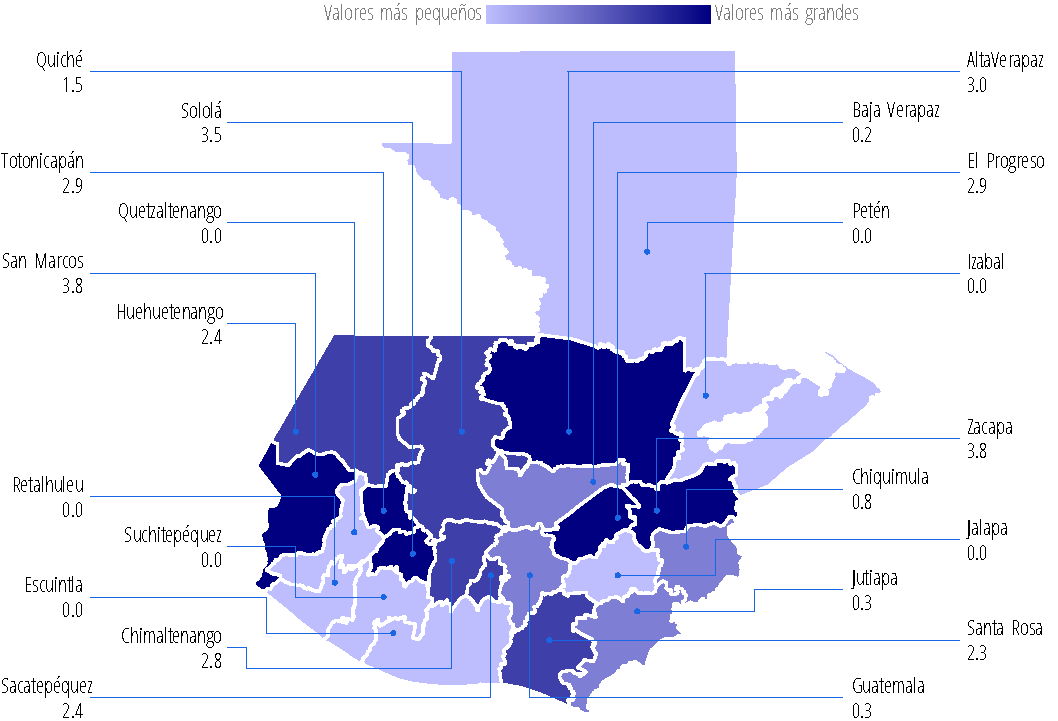
\includegraphics[width=52\cuadri]{graficas/diversificado/1_22.pdf} }{Instituto Nacional de Estadística, con datos del Ministerio de Educación}




\cajita{Aprobación}{La tasa de aprobación en diversificado se refiere a la cantidad de alumnos que culminaron y aprobaron el ciclo lectivo.
	
	Presentó el año 2009 el 76\% y en el  2014 fue de 83.1\%, aumento en 7.1 puntos porcentuales.}{Tasa de aprobación del ciclo de educación diversificada}{República de Guatemala, serie histórica, en porcentaje}{\ \\[0mm]\begin{tikzpicture}[x=1pt,y=1pt]  % Created by tikzDevice version 0.7.0 on 2015-08-28 13:12:27
% !TEX encoding = UTF-8 Unicode
\definecolor[named]{fillColor}{rgb}{1.00,1.00,1.00}
\path[use as bounding box,fill=fillColor,fill opacity=0.00] (0,0) rectangle (289.08,198.74);
\begin{scope}
\path[clip] (  0.00,  0.00) rectangle (289.08,198.74);
\definecolor[named]{drawColor}{rgb}{1.00,1.00,1.00}

\path[draw=drawColor,line width= 0.6pt,line join=round,line cap=round] (  0.00,  0.00) rectangle (289.08,198.74);
\end{scope}
\begin{scope}
\path[clip] (  0.00,  0.00) rectangle (289.08,198.74);

\path[] (  1.64, 17.78) rectangle (280.54,191.48);

\path[] (  1.64, 45.31) --
	(280.54, 45.31);

\path[] (  1.64, 84.60) --
	(280.54, 84.60);

\path[] (  1.64,123.88) --
	(280.54,123.88);

\path[] (  1.64,163.16) --
	(280.54,163.16);

\path[] (  1.64, 25.67) --
	(280.54, 25.67);

\path[] (  1.64, 64.95) --
	(280.54, 64.95);

\path[] (  1.64,104.24) --
	(280.54,104.24);

\path[] (  1.64,143.52) --
	(280.54,143.52);

\path[] (  1.64,182.80) --
	(280.54,182.80);

\path[] ( 33.83, 17.78) --
	( 33.83,191.48);

\path[] ( 87.46, 17.78) --
	( 87.46,191.48);

\path[] (141.09, 17.78) --
	(141.09,191.48);

\path[] (194.73, 17.78) --
	(194.73,191.48);

\path[] (248.36, 17.78) --
	(248.36,191.48);
\definecolor[named]{drawColor}{rgb}{0.00,0.00,1.00}

\path[draw=drawColor,line width= 1.7pt,line join=round] ( 33.83,151.38) --
	( 87.46,138.81) --
	(141.09,146.66) --
	(194.73,161.59) --
	(248.36,183.59);
\definecolor[named]{drawColor}{rgb}{0.00,0.00,0.00}

\node[text=drawColor,anchor=base,inner sep=0pt, outer sep=0pt, scale=  1.01] at ( 33.83,155.33) {76.0};

\node[text=drawColor,anchor=base,inner sep=0pt, outer sep=0pt, scale=  1.01] at ( 87.46,126.93) {74.4};

\node[text=drawColor,anchor=base east,inner sep=0pt, outer sep=0pt, scale=  1.01] at (137.98,146.66) {75.4};

\node[text=drawColor,anchor=base east,inner sep=0pt, outer sep=0pt, scale=  1.01] at (191.61,161.59) {77.3};

\node[text=drawColor,anchor=base,inner sep=0pt, outer sep=0pt, scale=  1.01] at (248.36,187.54) {80.1};
\definecolor[named]{fillColor}{rgb}{0.00,0.00,0.00}

\path[draw=drawColor,line width= 0.1pt,line join=round,fill=fillColor] (  1.64, 25.67) -- (280.54, 25.67);
\end{scope}
\begin{scope}
\path[clip] (  0.00,  0.00) rectangle (289.08,198.74);

\path[] (  1.64, 17.78) --
	(  1.64,191.48);
\end{scope}
\begin{scope}
\path[clip] (  0.00,  0.00) rectangle (289.08,198.74);

\path[] (  0.00, 25.67) --
	(  1.64, 25.67);

\path[] (  0.00, 64.95) --
	(  1.64, 64.95);

\path[] (  0.00,104.24) --
	(  1.64,104.24);

\path[] (  0.00,143.52) --
	(  1.64,143.52);

\path[] (  0.00,182.80) --
	(  1.64,182.80);
\end{scope}
\begin{scope}
\path[clip] (  0.00,  0.00) rectangle (289.08,198.74);

\path[] (  1.64, 17.78) --
	(280.54, 17.78);
\end{scope}
\begin{scope}
\path[clip] (  0.00,  0.00) rectangle (289.08,198.74);

\path[] ( 33.83, 13.51) --
	( 33.83, 17.78);

\path[] ( 87.46, 13.51) --
	( 87.46, 17.78);

\path[] (141.09, 13.51) --
	(141.09, 17.78);

\path[] (194.73, 13.51) --
	(194.73, 17.78);

\path[] (248.36, 13.51) --
	(248.36, 17.78);
\end{scope}
\begin{scope}
\path[clip] (  0.00,  0.00) rectangle (289.08,198.74);
\definecolor[named]{drawColor}{rgb}{0.00,0.00,0.00}

\node[text=drawColor,anchor=base,inner sep=0pt, outer sep=0pt, scale=  1.00] at ( 33.83,  2.85) {2009};

\node[text=drawColor,anchor=base,inner sep=0pt, outer sep=0pt, scale=  1.00] at ( 87.46,  2.85) {2010};

\node[text=drawColor,anchor=base,inner sep=0pt, outer sep=0pt, scale=  1.00] at (141.09,  2.85) {2011};

\node[text=drawColor,anchor=base,inner sep=0pt, outer sep=0pt, scale=  1.00] at (194.73,  2.85) {2012};

\node[text=drawColor,anchor=base,inner sep=0pt, outer sep=0pt, scale=  1.00] at (248.36,  2.85) {2014};
\end{scope}
  \end{tikzpicture}}{Instituto Nacional de Estadística, con datos del Ministerio de Educación}

\cajita{Aprobación por sexo}{La tasa de aprobación en diversificado por sexo fue del 80.2\% para hombres y 85.8\% para las mujeres.}{Tasa de aprobación del ciclo de educación diversificada, por sexo}{República de Guatemala, año 2014, en porcentaje}{\ \\[0mm]\begin{tikzpicture}[x=1pt,y=1pt]  % Created by tikzDevice version 0.10.1 on 2016-02-29 12:49:59
% !TEX encoding = UTF-8 Unicode
\definecolor{fillColor}{RGB}{255,255,255}
\path[use as bounding box,fill=fillColor,fill opacity=0.00] (0,0) rectangle (289.08,198.74);
\begin{scope}
\path[clip] (  0.00,  0.00) rectangle (289.08,198.74);

\path[] (  0.00,  0.00) rectangle (289.08,198.74);
\end{scope}
\begin{scope}
\path[clip] (  0.00,  0.00) rectangle (289.08,198.74);

\path[] (  0.00, 12.77) rectangle (289.08,181.67);

\path[] ( 54.20, 12.77) --
	( 54.20,181.67);

\path[] (144.54, 12.77) --
	(144.54,181.67);

\path[] (234.88, 12.77) --
	(234.88,181.67);
\definecolor{drawColor}{RGB}{0,0,255}
\definecolor{fillColor}{RGB}{0,0,255}

\path[draw=drawColor,line width= 0.6pt,line join=round,fill=fillColor] ( 36.13, 20.44) rectangle ( 72.27,169.16);

\path[draw=drawColor,line width= 0.6pt,line join=round,fill=fillColor] (126.47, 20.44) rectangle (162.61,163.99);

\path[draw=drawColor,line width= 0.6pt,line join=round,fill=fillColor] (216.81, 20.44) rectangle (252.95,173.99);
\definecolor{drawColor}{RGB}{0,0,0}

\path[draw=drawColor,line width= 0.1pt,line join=round] (  0.00, 20.44) -- (289.08, 20.44);

\node[text=drawColor,anchor=base,inner sep=0pt, outer sep=0pt, scale=  1.02] at ( 54.20,173.13) {83.1};

\node[text=drawColor,anchor=base,inner sep=0pt, outer sep=0pt, scale=  1.02] at (144.54,167.96) {80.2};

\node[text=drawColor,anchor=base,inner sep=0pt, outer sep=0pt, scale=  1.02] at (234.88,177.96) {85.8};

\path[] (  0.00, 12.77) rectangle (289.08,181.67);
\end{scope}
\begin{scope}
\path[clip] (  0.00,  0.00) rectangle (289.08,198.74);

\path[] (  0.00, 12.77) --
	(289.08, 12.77);
\end{scope}
\begin{scope}
\path[clip] (  0.00,  0.00) rectangle (289.08,198.74);

\path[] ( 54.20, 10.02) --
	( 54.20, 12.77);

\path[] (144.54, 10.02) --
	(144.54, 12.77);

\path[] (234.88, 10.02) --
	(234.88, 12.77);
\end{scope}
\begin{scope}
\path[clip] (  0.00,  0.00) rectangle (289.08,198.74);
\definecolor{drawColor}{RGB}{0,0,0}

\node[text=drawColor,anchor=base,inner sep=0pt, outer sep=0pt, scale=  1.00] at ( 54.20, -0.00) {Total};

\node[text=drawColor,anchor=base,inner sep=0pt, outer sep=0pt, scale=  1.00] at (144.54, -0.00) {Hombre};

\node[text=drawColor,anchor=base,inner sep=0pt, outer sep=0pt, scale=  1.00] at (234.88, -0.00) {Mujer};
\end{scope}
  \end{tikzpicture}}{Instituto Nacional de Estadística, con datos del Ministerio de Educación}

\cajota{Aprobación en los departamentos}{El mapa muestra en color celeste los departamentos con las menores tasas de aprobación en diversificado en el 2013 fueron:  Quetzaltenango 80.7\%, San Marcos 80.3\% y Alta Verapaz 75.6\%.
	
	 Los departamentos con las mayores tasas de aprobación en diversificado fueron: Huehuetenango 88.5\%, Chiquimula 87.0\% y Jutiapa 86.5\%. El departamento de Guatemala presentó una tasa de aprobación de 82.8\%.}{Tasa de aprobación del ciclo de educación diversificada}{Por departamento, año 2014, en porcentaje}{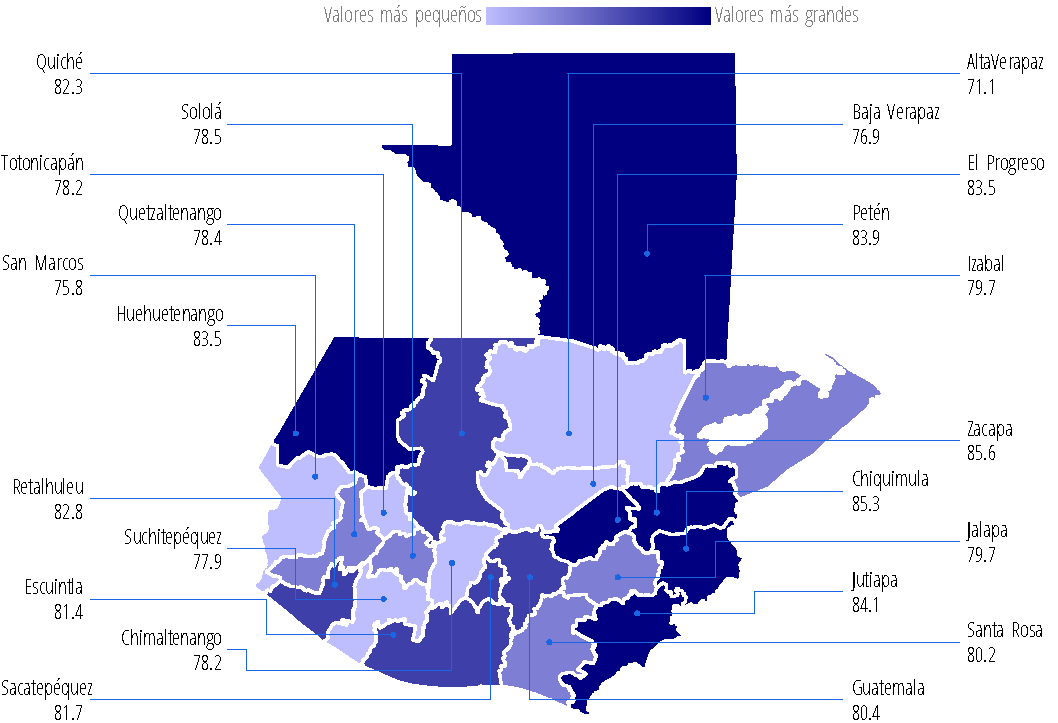
\includegraphics[width=52\cuadri]{graficas/diversificado/1_25.pdf} }{Instituto Nacional de Estadística, con datos del Ministerio de Educación}




%
%
%\INEpartecarta{Estadísticas de educación superior}{}
%
%\INEchaptercarta[Matriculados en educación superior]{Matriculados \\en educación superior}{}


\cajita{Matriculados}{La educación superior o terciaria, se desarrolla sobre la base de los conocimientos adquiridos en la educación secundaria, incluye también la educación vocacional o profesional avanzada. El número de matriculados en educación superior, se obtiene del total de  estudiantes inscritos en los sectores público y privado.\\ 
	
	 En la presente gráfica en serie de años, se observa que en el año 2009 se matricularon 216,884 y en el año 2014 lo hicieron 313,457, lo cual muestra un crecimiento de  44.5\%.}{Matriculados en universidades}{República de Guatemala, serie histórica, en datos absolutos}{\ \\[0mm]}{Instituto Nacional de Estadística}


\cajita{Crecimiento matriculados}{En la presente gráfica, se observa que el crecimiento de la matrícula de los años 2009 a 2012 tuvo un comportamiento relativamente similar, mostrando un crecimiento no mayor del 7.6\%, pero la matricula del año 2012 al año 2014 creció de 5.4\% a 18.7\%.}{Tasa de crecimiento de estudiantes universitarios}{República de Guatemala, serie histórica, en porcentaje}{\ \\[0mm]}{Instituto Nacional de Estadística}


\cajita{Matriculados en sector privado}{En la presente gráfica se observa que en el sector privado de educación superior, en el año 2009 la proporción de estudiantes fue de 38.1\% y para el año 2014 fue de 42.1\%, observándose un crecimiento de 10.5\%.}{Proporción de estudiantes universitarios que se inscribieron en universidades del sector privado}{República de Guatemala, serie histórica, en porcentaje}{\ \\[0mm]}{Instituto Nacional de Estadística}

\cajita{Tipo de ingreso}{De los estudiantes matriculados en educación superior, el 79.8\% son de reingreso.}{Distribución de estudiantes universitarios inscritos según el tipo de matrícula}{República de Guatemala, 2014, datos absolutos}{\ \\[0mm]}{Instituto Nacional de Estadística}
	

\cajita{Mujeres matriculadas}{En la gráfica se observa que en el año 2004, de cada cien matriculados,  cuarenta y seis eran mujeres, en el año 2014, de cada cien matriculados cincuenta eran mujeres.}{Proporción de estudiantes universitarios que son mujeres}{República de Guatemala, serie histórica, en porcentaje}{\ \\[0mm]}{Instituto Nacional de Estadística}


\cajita{Crecimiento matriculados por sexo}{En el año 2010 y 2011, el crecimiento fue mayor para los hombres, a partir del año 2012 el crecimiento fue mayor en mujeres.}{Tasa de crecimiento de estudiantes \\ universitarios, por sexo}{República de Guatemala, serie histórica, en porcentaje}{\ \\[0mm]}{Instituto Nacional de Estadística}


\cajita{Edad de los matriculados}{En la distribución de matriculados por edad, en el año 2014, el 34.8\% pertenecían al grupo de 20 a 24 años y el 23.1\% eran del grupo de 25 a 29 años, un 10.5\% no fue posible determinar la edad de matriculación.}{Distribución de estudiantes universitarios, por grupo de edad}{República de Guatemala, 2014, en porcentaje}{\ \\[0mm]}{Instituto Nacional de Estadística}


\cajita{Edad y sexo de los matriculados}{En la siguiente gráfica, se observa que en el grupo de matriculados de 20 a 24 años, el 38.1\% eran hombres y 39.6\% mujeres, en el grupo de 25 a 29 años el 25.7\% eran hombres y 25.9 mujeres.\\
	
	 En el grupo de 15 a 19 años, el 5.3\% eran hombres y el 5.8\% mujeres.}{Distribución de estudiantes universitarios \\por sexo y según grupo de edad}{República de Guatemala, 2014, en porcentaje}{\ \\[0mm]}{Instituto Nacional de Estadística}


\cajita{Matriculados nuevos por sexo}{La distribución de matriculados nuevos por sexo indica que 51.3\% son hombres y 48.7\% mujeres, siendo la diferencia de 2.6 puntos porcentuales.}{Distribución de estudiantes universitarios nuevos  por sexo}{República de Guatemala, 2014, en porcentaje}{\ \\[0mm]}{Instituto Nacional de Estadística}


\cajita{Edad de los matriculados nuevos}{En la presente gráfica se observa que los matriculados nuevos, en el grupo de 20 a 24 años tiene el 40\%, es importante observar que el grupo de 15 a 19 años presenta el 19\%, superior al grupo de 25 a 29 años que es de 14.3\%.\\ 
	
	 De los matriculados nuevos un 14.3\% no fue posible determinar la edad.}{Distribución de estudiantes universitarios nuevos  por grupo de edad}{República de Guatemala, 2014, en porcentaje}{\ \\[0mm]}{Instituto Nacional de Estadística}




\cajita{Grado académico}{En la presente gráfica, se observa que los matriculados en nivel técnico y licenciatura es de 95\% mientras que los del nivel de doctorado y equivalente es de 0.2\%.}{Distribución de los estudiantes universitarios por nivel}{República de Guatemala, 2014, en porcentaje}{\ \\[0mm]}{Instituto Nacional de Estadística}


\cajita{Grado académico en la universidad pública}{De cada 100 matriculados universitarios que estudian en el nivel técnico o licenciatura, 59 estudian en la universidad estatal.
	
	Asimismo, por cada 100 estudiantes que estudian maestría, 43 están en la Universidad de San Carlos y 70 por cada 100 de doctorado.}{Proporción de estudiantes universitarios que se matricularon en la universidad estatal, por nivel}{República de Guatemala, 2014, en porcentaje}{\ \\[0mm]}{Instituto Nacional de Estadística}

\cajita{Mujeres según grado académico}{Por cada 100 matriculados en el nivel técnico y licenciatura, 51 son mujeres.\\
	
	Asimismo, en maestría, por cada 100 estudiantes, 49 son mujeres; y en doctorado, 37.}{Proporción de estudiantes universitarios que son  mujeres, por nivel}{República de Guatemala, 2014, en porcentaje}{\ \\[0mm]}{Instituto Nacional de Estadística}


\cajita{Campo de estudio}{La distribución de matriculados por campos de estudio, para las ciencias sociales, son 64.3\%, en las humanidades el porcentaje es de 14.8\% y en las ciencias naturales el 1\%.}{Distribución de estudiantes universitarios por campo de estudio}{República de Guatemala, 2014, en porcentaje}{\ \\[0mm]}{Instituto Nacional de Estadística}


\cajita{Estudiantes en la universidad pública, por campo de estudio }{La gráfica muestra el porcentaje de matriculados en la universidad estatal en relación al campo de estudio.
	
	Así, en la Universidad de San Carlos se encuentra inscrito el 100\% de estudiantes que cursan carreras del campo de ciencias agrícolas; de las carreras en el campo de ciencias naturales, el 80.7\%.
		
	En el campo de Ingeniería y Tecnología, el 45\% de estudiantes se inscribieron en la Universidad de San Carlos.}{Proporción de estudiantes universitarios que se matricularon en la universidad estatal, por campo de estudio}{República de Guatemala, 2014, en porcentaje}{\ \\[0mm]}{Instituto Nacional de Estadística}

\cajita{Mujeres según campo de estudio}{La gráfica muestra el porcentaje de matriculados mujeres en relación al total de estudiantes según el campo de estudio.
	
	Así, se encuentra que el 68.5\% de los estudiantes inscritos en carreras de ciencias naturales, son mujeres; en humanidades, el 66.4\% son mujeres.
		
	En el campo de Ingeniería y Tecnología, el 22.2\% de estudiantes que se inscribieron son mujeres.}{Proporción de estudiantes universitarios que son mujeres, por campo de estudio}{República de Guatemala, 2014, en porcentaje}{\ \\[0mm]}{Instituto Nacional de Estadística}



%\cajita{--}{}{--}{República de Guatemala, 2014, en porcentaje}{\ \\[0mm]\begin{tikzpicture}[x=1pt,y=1pt]  \input{C:/Users/INE/Desktop/compendio_educacion/graficas/matriculau/1_.tex}  \end{tikzpicture}}{Instituto Nacional de Estadística}

%
%\INEchaptercarta[Graduados de educación superior]{Graduados \\de educación superior}{}

\cajita{Graduados}{El término graduado de educación superior, se refiere al estudiante que culminó exitosamente un programa educativo. 
	
	En la presente gráfica en serie de años, se observa que en el año 2009 se graduaron  9,594 y en el año 2014 lo hicieron 24,442, lo cual muestra un crecimiento de  155.8\%.}{Graduados de educación superior}{República de Guatemala, serie histórica, datos absolutos}{\ \\[0mm]}{Instituto Nacional de Estadística}

\cajita{Mujeres graduadas}{Del total de graduados en el 2009, el 53.4\% eran mujeres y para el año 2014 fueron 55.7\%, aumentando en 2.3 puntos porcentuales, 5 años después.}{Proporción de graduados de educación superior que son mujeres }{República de Guatemala, serie histórica, en porcentaje}{\ \\[0mm]}{Instituto Nacional de Estadística}

\cajita{Grado obtenido}{Los graduados en el año 2014, en el nivel técnico, licenciatura y equivalente fue el 89.2\%, mientras que en la maestría únicamente fue el 0.1\%.}{Distribución de graduados de educación superior según el nivel obtenido}{República de Guatemala, 2014, en porcentaje}{\ \\[0mm]}{Instituto Nacional de Estadística}

\cajita{Grado obtenido según sexo}{ En el año 2014, del nivel donde más egresaron académicos, fue de técnico, licenciatura o equivalente, donde el porcentaje de hombres fue de 88\% y el de mujeres el 90\%.}{Distribución de los graduados por sexo, según el nivel obtenido}{República de Guatemala, 2014, en porcentaje}{\ \\[0mm]}{Instituto Nacional de Estadística}


\cajita{Graduados según campo de estudio}{De los campos de educación superior, del total de egresados el 57.2\% se graduaron de carreras de las Ciencias Sociales. Las Ciencias Agrícolas representaron el 0.6\%.}{Distribución de graduados de educación superior\\ según el campo de estudio}{República de Guatemala, 2014, en porcentaje}{\ \\[0mm]}{Instituto Nacional de Estadística}


\cajita{Graduados según campo de estudio y sector}{De los sectores público y privado, los egresados por campos científicos en su mayoría fue de las Ciencias Sociales y de las humanidades.}{Distribución porcentual de los graduados  de educación superior según el campo de estudio, por sector}{República de Guatemala, 2014, en porcentaje}{\ \\[0mm]}{Instituto Nacional de Estadística}


%
%\INEpartecarta{Educación y fecundidad}{}
%
%\INEchaptercarta{Nacimientos: características escolares de las madres}{}

\cajita{Nacimientos}{La cantidad de nacimientos registrados en el 2014 tuvo una disminución del 0.32\% respecto al año anterior.}{Nacimientos registrados}{República de Guatemala, serie histórica, en datos absolutos}{\ \\[0mm]}{Instituto Nacional de Estadística}

\cajita{Escolaridad de la madre}{De los nacimientos ocurridos en el 2014, el 37.5\% fueron en madres con escolaridad en el nivel primario; el 31.2\% en mujeres sin ningún nivel de escolaridad.}{Distribución de los nacimientos según escolaridad de la madre }{República de Guatemala, 2014, en porcentaje}{\ \\[0mm]}{Instituto Nacional de Estadística}

\cajita{Madres sin escolaridad}{La proporción de nacimientos en madres sin escolaridad ha tenido una tendencia descendente, de 37.8\% a 31.2\%, en el período 2010-2014.}{Proporción de nacimientos en madres sin escolaridad}{República de Guatemala, serie histórica, en porcentaje}{\ \\[0mm]}{Instituto Nacional de Estadística}

\cajita{Madres sin escolaridad por etnia}{La proporción de nacimientos en madres sin escolaridad según su grupo étnico es del 45\% en las madres indígenas, no tenían ningún nivel de escolaridad. De las madres no indígenas era el 16.5\%.}{Proporción de nacimientos en madres sin escolaridad}{República de Guatemala, serie histórica, en porcentaje}{\ \\[0mm]}{Instituto Nacional de Estadística}

\cajota{Madres sin escolaridad en los departamentos}{Los departamentos que reportan un mayor porcentaje de nacimientos en madres sin escolaridad son de la región II: Alta Verapaz y Baja Verapaz; de la región VI:  Totonicapán y Sololá; de la región VII: Quiché; y de la región IV: Zacapa.\\
	
	 Los departamentos con menor porcentaje fueron Guatemala, El Progreso, Chimaltenango, Sacatepéquez, Escuintla y Santa Rosa.}{Proporción de nacimientos en madres sin escolaridad }{Departamental, 2014, en porcentaje}{}{Instituto Nacional de Estadística}

\cajita{Promedio de hijos***}{Las madres que tuvieron un nacimiento en el 2014, aquellas sin ningún nivel de escolaridad tenían en promedio 3.7 hijos y las madres con nivel de posgrado, 1.6 hijos.}{Promedio de hijos por madre al momento del nuevo nacimiento, según su escolaridad}{República de Guatemala, 2014, en porcentaje}{\ \\[0mm]}{Instituto Nacional de Estadística}

\cajita{Promedio de hijos de madres sin escolaridad}{Según los nacimientos reportados cada año, las madres sin ningún nivel de educación han tenido, al momento del nuevo nacimiento, un promedio de 3.7 hijos.}{Promedio de hijos por madre sin educación,\\ al momento del nuevo nacimiento}{República de Guatemala, serie histórica, en porcentaje}{\ \\[0mm]}{Instituto Nacional de Estadística}


\cajota{Promedio de hijos de madres sin escolaridad en los departamentos}{Según los nacimientos reportados en el 2014, las madres sin ningún nivel de escolaridad, tenían en promedio 3.7 hijos.\\
	
	 Los departamentos con el mayor número de hijos, en promedio, fueron Quiché y Sololá.}{Promedio de hijos por madre sin educación, al momento del nuevo nacimiento}{Departamental, 2014, en porcentaje}{}{Instituto Nacional de Estadística}

\cajita{Madres que recibieron atención médica}{Los nacimientos ocurridos en el 2014, el 98.5\% de las madres con educación superior recibió asistencia médica, por otro lado, solo el 42.6\% de las madres sin educación tuvo este tipo de atención médica.}{Proporción de nacimientos que recibieron atención médica según nivel de escolaridad de la madre}{República de Guatemala, 2014, en porcentaje}{\ \\[0mm]}{Instituto Nacional de Estadística}

\cajita{Madres sin escolaridad que recibieron atención médica}{La tendencia de los nacimientos en madres sin educación que reciben atención médica ha sido ascendente.}{Proporción de nacimientos en madres sin educación, que recibieron atención médica}{República de Guatemala, serie histórica, en porcentaje}{\ \\[0mm]}{Instituto Nacional de Estadística}


\cajota{Madres sin escolaridad que recibieron atención médica\newline en los departamentos}{Los departamentos con menor proporción de nacimientos que recibieron atención médica, en madres sin educación fueron: Huehuetenango (20.4\%), San Marcos (29.4\%), Quiché (25.3\%), Totonicapán (30.5\%) y Sololá (35.0\%).}{Proporción de nacimientos de madres sin escolaridad que recibieron atención médica}{Departamental, 2014, en porcentaje}{}{Instituto Nacional de Estadística}


\cajita{Nacimientos ocurridos en centro médico, según escolaridad la madre}{\footnote{Incluye los nacimientos ocurridos en: hospital privado, hospital público, centro de salud e IGSS} Los nacimientos ocurridos en el 2014, el 97.1\% de las madres con educación superior recibió atención en un centro médico, por otro lado, solo el 43.4\% de las madres sin educación tuvo atención médica en este tipo de centro.}{Proporción de nacimientos que ocurrieron en centro médico, según el nivel de escolaridad de la madre}{República de Guatemala, 2014, en porcentaje}{\ \\[0mm]}{Instituto Nacional de Estadística}

\cajita{Nacimientos ocurridos en centro médico, madres sin escolaridad***}{La tendencia de los nacimientos en madres sin educación que reciben atención en un centro médico ha sido ascendente.}{Proporción de nacimientos en madres sin escolaridad, que ocurrieron en centros de atención médica}{República de Guatemala, serie histórica, en porcentaje}{\ \\[0mm]}{Instituto Nacional de Estadística}

\cajota{Madres sin escolaridad que recibieron atención médica\newline en los departamentos}{Los departamentos con menor proporción de nacimientos en madres sin educación  que recibieron atención en un centro médico, fueron: Huehuetenango (20.8\%), San Marcos (29.2\%), Quiché (25.4\%), Totonicapán (30.3\%) y Sololá (34.1\%).}{Nacimientos en madres sin educación que recibieron atención médica}{Departamental,2014, en porcentaje}{}{Instituto Nacional de Estadística}

%
%
%
%\INEpartecarta{Gasto en educación}{}
%
%\INEchaptercarta[Gasto público y financiamiento]{Gasto público y\\ financiamiento}{}


\cajita{Evolución del gasto, por sector}{El gasto público en educación en el 2014 fue de Q12,896, del cual el 83.3\% se destinó a entidades centralizadas. En el 2012 fue asignado a este sector el 83.6\%.\\
	
	\textollamada[*]{ Dentro este tipo de entidades se encuentra: el Ministerio de Educación, Ministerio de la Defensa, Ministerio de Salud Pública y Asistencia Social y el Ministerio de Agricultura, Ganadería y Alimentación.}}{Gasto público en educación, por sector}{República de Guatemala, 2012 y 2014, en millones de quetzales de cada año}{
		\ra{1.2}$\ $\\
		\begin{tabular}{p{3.5cm}x{2cm}x{2cm}}\hline
		\rowcolor{color2!15!white} &&\\[-4mm]
		{\Bold    Sector          }&      \textbf{ 2012 }  &  \textbf{ 2014 }   \\
		\hline
		\rowcolor{white} &&\\[-4mm]
		
	\textbf{Total general} &	\textbf{12,133}& 	\textbf{12,896} \\
	Centralizadas&	10,147& 	10,749 \\
	Descentralizadas&	1,986 &	2,148 \\
		\hline
		&&\\[2mm]
		\end{tabular}
		}{Instituto Nacional de Estadística, ICEFI con datos de SICOIN del  2012, 2014.}


\cajita{Gasto por sector}{Según el sector de las entidades en educación, estas son centralizadas o descentralizadas. En el año 2014 el 16.7\% de los recursos del gasto público en educación fue asignado a las entidades descentralizadas.\\
	
	Entre las entidades descentralizadas se incluye: la Universidad de San Carlos de Guatemala, el Instituto Técnico de Capacitación y Productividad, el Comité Nacional de Alfabetización y la Escuela Nacional Central de Agricultura.}{Distribución de gasto público, por sector}{República de Guatemala, 2014, en porcentaje}{\ \\[0mm]}{Instituto Nacional de Estadística, ICEFI con datos de SICOIN del  2014.}


\cajita{Crecimiento del gasto en educación}{El gasto público en educación asignado a entidades descentralizadas tuvo un crecimiento de 8.1\%. \textollamada[*]{La tasa de crecimiento se calculó utilizando quetzales corrientes de 2012 y 2014.}}{Tasa de crecimiento anual del gasto público en educación, por sector}{República de Guatemala, 2014, en porcentaje}{\ \\[0mm]}{Instituto Nacional de Estadística, ICEFI con datos de SICOIN del 2012 y 2014.}


\cajita{Evolución del gasto en educación, por entidad}{Del gasto público total asignado en el 2014, el Ministerio de Educación recibió un 78\%. En el 2012 había recibido el 77\%.\\
	
	La segunda y tercer mayor asignación fue para dos entidades descentralizadas, la Universidad de San Carlos de Guatemala (que  tuvo un crecimiento presupuestario del 4\% respecto al 2012)\textollamada[*]{Los cálculos están realizados en quetzales corrientes de cada año.}, y el Instituto Técnico de Capacitación y Productividad.}{Gasto público en educación, por entidad}{República de Guatemala, 2012 y 2014, en millones de quetzales de cada año}{
	\ra{1.2}$\ $\\
	\begin{tabular}{p{6cm}rr}\hline
		\rowcolor{color2!15!white} &&\\[-4mm]
		{\Bold    Entidad          }&       \textbf{2012}   &   \textbf{2014}    \\
		\rowcolor{white} &&\\[-4mm]
		
	\textbf{	Total }&\textbf{	12,133} &\textbf{	12,896} \\
	Ministerio de Educación	& 9,342 &	10,003 \\
		Universidad de San Carlos&	1,568 &	1,627 \\
		Instituto Técnico de Capacitación y Productividad&	230 &	256 \\
		Obligaciones del Estado a cargo del Tesoro&	279 &	189 \\
		Comité Nacional de Alfabetización&	129 &	188 \\
		Ministerio de la Defensa Nacional&	159 &	182 \\
		Ministerio de Salud Pública y Asistencia Social&	178 &	154 \\
		Ministerio de Gobernación&	60& 	129 \\
		Escuela Nacional Central de Agricultura&	33& 	46 \\
		Resto de entidades&	155&	122\\
		
		\hline
		\rowcolor{white} &&\\[-5.5mm]

		&&\\[-0.09cm]
	\end{tabular}}{Instituto Nacional de Estadística, ICEFI con datos de SICOIN del 2012 y 2014.}


\cajita{Gasto por entidad}{Del total de gasto público en educación asignado a entidades centralizadas (83.3\% del total de gasto público), el 93\% se destina al Ministerio de Educación.
	
	 Del mismo El 22.4\% del gasto público en educación es asignado a las La distribución porcentual del gasto público en educación }{Distribución del gasto público en educación por entidad}{República de Guatemala, 2014, en porcentaje}{\ \\[0mm]}{Instituto Nacional de Estadística, ICEFI con datos de SICOIN del 2012 y 2014.}


\cajita{Crecimiento del gasto en educación por entidad}{De las entidades con mayor erogación de gasto público, tuvieron  mayor crecimiento de gasto, respecto al 2012, el Ministerio de Gobernación con el 115.7\%, seguido del Comité Nacional de Alfabetización 45.7\%. 
	
\textollamada[*]{La tasa de crecimiento se calculó utilizando quetzales corrientes de 2012 y 2014.}	Las entidades con mayor decrecimiento fueron las obligaciones del Estado a cargo del Tesoro 32.2\% y el Ministerio de Salud Pública y Asistencia Social 13.1\%.}{Tasa de crecimiento anual del gasto público en educación, por entidades con mayor erogación}{República de Guatemala, 2014, en porcentaje}{\ \\[0mm]}{Instituto Nacional de Estadística, ICEFI con datos de SICOIN del 2012 y 2014.}


\cajita{Evolución del gasto en educación, por grupo}{Según el grupo de gasto, el pago en servicios personales y no personales abarcó en el 2014 el 84\% del gasto público en educación. \\
	
	El grupo de gasto de materiales y suministro tuvo una disminución del 31\% respecto a la asignación del 2012.}{Gasto público en educación, por grupo de gasto}{República de Guatemala, 2012 y 2014, en millones de quetzales de cada año}{
	\ra{1.2}$\ $\\
	\begin{tabular}{p{6cm}rr}\hline
		\rowcolor{color2!15!white} &&\\[-4mm]
		{\Bold    Grupo de gasto         }&      \textbf{2012}   &  \textbf{2014}    \\
\hline
		\rowcolor{white} &&\\[-4mm]
		
\textbf{	Total}&	\textbf{12,133}& 	\textbf{12,896 }\\
	Servicios Personales&	9,344 &	10,272 \\
	Servicios No Personales&	653 &	597 \\
	Materiales y Suministros&	859 &	590 \\
	Propiedad, Planta, Equipo e Intangibles&	207& 	204 \\
	Transferencias Corrientes&	777 &	1,027 \\
	Transferencias de Capital&	276 &	189 \\
	Asignaciones Globales&	16 &	17 \\
			\hline
		\rowcolor{white} &&\\[-5.5mm]
	
		&&\\[-0.09cm]
	\end{tabular}}{Instituto Nacional de Estadística, ICEFI con datos de SICOIN del 2012 y 2014.}


\cajita{Gasto en educación por grupo}{El rubro más importante, en relación a la cantidad en la asignación de gasto, ha sido el pago de servicios personales, que representa el 79.7\% del total del gasto público en educación. Los materiales y suministros representaron el 4.6\% del gasto total.}{Distribución del gasto público en educación por grupo de gasto}{República de Guatemala, 2014, en porcentaje}{\ \\[0mm]}{Instituto Nacional de Estadística, ICEFI con datos de SICOIN del 2012 y 2014.}


\cajita{Crecimiento del gasto en educación por grupo}{\textollamada[*]{Los cálculos están realizados en quetzales corrientes de cada año.}El rubro que tuvo un mayor crecimiento de gasto, respecto al 2012, fueron las transferencias corrientes, con el 32.2\%, seguido de los servicios personales con el 9.9\%. El rubro con el mayor decrecimiento fueron las transferencias de capital, con el 31.5\% y el rubro de materiales y suministros con el 31.4\%.}{Tasa de crecimiento anual del gasto público en educación por grupo de gasto}{República de Guatemala, 2014, en porcentaje}{\ \\[0mm]}{Instituto Nacional de Estadística, ICEFI con datos de SICOIN del 2012 y 2014.}


\cajita{Evolución del gasto en educación, por tipo}{El gasto público en educación se puede dividir en gastos corrientes y gastos de capital. En el corriente se incluyen el pago de salarios a funcionarios, compras de bienes y servicios, el cual representó 97\% de la asignación en gasto en educación.}{Gasto público en educación por tipo de gasto}{República de Guatemala, 2012 y 2014, en millones de quetzales de cada año}{
	\ra{1.2}$\ $\\
	\begin{tabular}{p{6cm}rr}\hline
		\rowcolor{color2!15!white} &&\\[-4mm]
		{\Bold    Tipo de gasto         }&     \textbf{  2012 }  &  \textbf{ 2014 }   \\
		\hline
		\rowcolor{white} &&\\[-4mm]
		
	\textbf{Total}&	\textbf{12,133}&	\textbf{12,896}\\
	Gastos Corrientes&	11,649	& 12,499\\
	Gastos de Capital&	484	& 398\\	
		\hline
		\rowcolor{white} &&\\[-5.5mm]
		&&\\[-0.09cm]
	\end{tabular}}{Instituto Nacional de Estadística, ICEFI con datos de SICOIN del 2012 y 2014.}


\cajita{Gasto en educación por tipo}{\textollamada[*]{Los cálculos están realizados en quetzales corrientes de cada año.}La distribución porcentual del gasto público en educación según su tipo, muestra que el 96.9\% fue asignado a gastos corrientes y el 3.2\% a gasto de capital.}{Distribución del gasto en educación por tipo de gasto}{República de Guatemala, 2014, en porcentaje}{\ \\[0mm]}{Instituto Nacional de Estadística, ICEFI con datos de SICOIN del 2012 y 2014.}


\cajita{Crecimiento del gasto en educación por tipo}{El gasto público en educación tuvo un crecimiento del  6.4\%. La división de este según el tipo, los gastos de capital tuvieron una disminución del 17.8\% respeto al 2012. Mientras que los gastos corrientes tuvieron un aumento del 7.3\%}{Tasa de crecimiento anual del gasto público en educación por tipo de gasto}{República de Guatemala, 2014, en porcentaje}{\ \\[0mm]}{Instituto Nacional de Estadística, ICEFI con datos de SICOIN del 2012 y 2014.}


\cajita{Evolución del gasto en educación por función}{Según la función en la que fue invertido el presupuesto,  el sector más impactado fue la educación preprimaria y primaria, que  representó el 53\% del presupuesto total y tuvo un crecimiento del 4.3\%. La educación media, tuvo una asignación del 12\% y un crecimiento del 4.7\%.  Asimismo, la educación superior tuvo un 13\% y un decrecimiento del 5.2\%.}{Gasto público en educación por función}{República de Guatemala, 2012 y 2014, en millones de quetzales de cada año	}{
	\ra{1.2}$\ $\\
	\begin{tabular}{p{7.5cm}rr}\hline
		\rowcolor{color2!15!white} &&\\[-4mm]
		{\Bold   Función         }&      \textbf{ 2012}   &  \textbf{ 2014   } \\
		\hline
		\rowcolor{white} &&\\[-4mm]
		
\textbf{Total}&	\textbf{12,133}& 	\textbf{12,896 }\\
Educación preprimaria y primaria&	6,609 &	6,894 \\
Servicios auxiliares de la educación&	1,273& 	1,725 \\
Educación universitaria o superior	&1,721 &	1,632 \\
Educación media	& 1,436 &	1,504 \\
Educación n.c.d &	624 &	662 \\
Educación no atribuible a ningún nivel escolarizado &	420 &	445 \\
Investigación y desarrollo relacionados con la educación&	23& 	25 \\
Educación postmedia básica y diversificado no universitaria&	27 &	9 \\

		\hline
		\rowcolor{white} &&\\[-5.5mm]
	
		&&\\[-0.09cm]
	\end{tabular}}{Instituto Nacional de Estadística, ICEFI con datos de SICOIN del 2012 y 2014.}


\cajita{Gasto en educación por función}{La función con mayor incidencia  en relación a la asignación de gasto, ha sido la educación preprimaria y primaria, que representa el 53.5\% del total del gasto público en educación. El que tuvo la menor incidencia fue  el gasto en educación postmedia básica y diversificada, con el 0.1\% del gasto total.}{Distribución del gasto público en educación, por función}{República de Guatemala, 2014, en porcentaje}{\ \\[0mm]}{Instituto Nacional de Estadística, ICEFI con datos de SICOIN del 2012 y 2014.}


\cajita{Crecimiento del gasto en educación por función}{
	La función que tuvo el mayor crecimiento de gasto, respecto al 2012, fueron los servicios auxiliares de educación, con el 35.5\%, seguido de la investigación y desarrollo en educación con el 9.5\%. \\
	
	El rubro con el mayor decrecimiento en la asignación de gasto fue la educación postmedia básica y diversificado, con el 68.1\% y la educación universitaria con el 5.2\%, respecto al año anterior.
	}{Tasa de crecimiento anual del gasto público en educación por función}{República de Guatemala, 2014, en porcentaje}{\ \\[0mm]}{Instituto Nacional de Estadística, ICEFI con datos de SICOIN del 2012 y 2014.}


\cajita{Evolución de las fuentes de financiamiento}{De acuerdo a la fuente de financiamiento, la mas importante provino de recursos del tesoro (con y sin afectación específica) de donde se obtuvo el 95\% del presupuesto y este tuvo aumento del 13\% respecto del año anterior. El 0.26\% del gasto público en educación provino de donaciones externas.}{Gasto público en educación por fuente de financiamiento agregada}{República de Guatemala, 2012 y 2014, en millones de quetzales de cada año}{
	\ra{1.2}$\ $\\
	\begin{tabular}{p{6cm}rr}\hline
		\rowcolor{color2!15!white} &&\\[-4mm]
		{\Bold   Fuente de financiamiento         }&      \textbf{ 2012}   &  \textbf{ 2014 }   \\
		\hline
		\rowcolor{white} &&\\[-4mm]
		
	\textbf{	Total}&	\textbf{12,133}& 	\textbf{12,896}  \\
	Recursos del Tesoro&	7,625 &	8,912  \\
		Recursos del Tesoro con Afectación Especifica&	3,194 &	3,342  \\
		Recursos Propios de las Instituciones&	387 & 378  \\
		Crédito Externo&	877 &	231  \\
		Donaciones Externas&	50 	& 33  \\
		
		\hline
		\rowcolor{white} &&\\[-5.5mm]

		&&\\[-0.09cm]
	\end{tabular}}{Instituto Nacional de Estadística, ICEFI con datos de SICOIN del 2012 y 2014.}


\cajita{Fuentes de financiamiento}{La fuente de financiamiento con mayor incidencia  en relación a la asignación obtenida, fueron los recursos del tesoro, que representó el 69.1\% del total del gasto público en educación. El que tuvo la menor incidencia fueron las donaciones externas, con el  0.3\% del financiamiento en gasto público en educación total.}{Distribución del gasto público en educación por fuente de financiamiento agregada}{República de Guatemala, 2014, en porcentaje}{\ \\[0mm]}{Instituto Nacional de Estadística, ICEFI con datos de SICOIN del 2012 y 2014.}


\cajita{Crecimiento de la fuentes de financiamiento}{La fuente de financiamiento que tuvo el mayor crecimiento de asignación, respecto al 2012, fueron los recursos del tesoro, con el 16.9\%, seguido de los recursos del tesoro con afectación específica, con el 4.6\%.\\
	
	 El rubro con el mayor decrecimiento en el financiamiento del gasto público en educación  fue el crédito externo, con el 73.6\% y las donaciones externas, con el 34.6\%, respecto al año anterior.}{Tasa de crecimiento anual del gasto público en educación por fuente de financiamiento agregada}{República de Guatemala, 2014, en porcentaje}{\ \\[0mm]}{Instituto Nacional de Estadística, ICEFI con datos de SICOIN del 2012 y 2014.}


\cajita{Gasto en educación en relación al PIB}{El gasto público en educación como porcentaje del producto interno bruto tuvo una variación de 0.1 puntos porcentuales, respecto del 2012.
	Asimismo, en el 2014 de la totalidad del gasto público, el 21.3\% fue asignado para educación, teniendo un aumento de 0.3 puntos porcentuales respecto al 2012.
	}{Gasto público en educación como porcentaje del producto interno bruto y el gasto público}{República de Guatemala, 2012 y 2014, en porcentaje}{\ \\[0mm]}{Instituto Nacional de Estadística, ICEFI con datos de SICOIN del 2012 y 2014.}















\INEpartecarta{Educación y empleo}{}


\INEchaptercarta{Alfabetismo de la población en edad de trabajar}{}


\cajita{Alfabetismo}{La tasa de alfabetismo de las personas en edad de trabajar, relaciona a la población mayor de 14 años que sabe leer y escribir respecto al total de la población en edad de trabajar, esta se ha situado entre el  75.7 y 81.3\%.}{Tasa de alfabetismo en personas mayores de 14 años}{República de Guatemala, serie histórica, en porcentaje}{\ \\[0mm]\begin{tikzpicture}[x=1pt,y=1pt]  % Created by tikzDevice version 0.9 on 2015-12-11 10:47:29
% !TEX encoding = UTF-8 Unicode
\definecolor{fillColor}{RGB}{255,255,255}
\path[use as bounding box,fill=fillColor,fill opacity=0.00] (0,0) rectangle (289.08,198.74);
\begin{scope}
\path[clip] (  0.00,  0.00) rectangle (289.08,198.74);

\path[] (  0.00,  0.00) rectangle (289.08,198.74);
\end{scope}
\begin{scope}
\path[clip] (  0.00,  0.00) rectangle (289.08,198.74);

\path[] (  1.64, 17.78) rectangle (280.54,191.48);

\path[] (  1.64, 45.10) --
	(280.54, 45.10);

\path[] (  1.64, 83.95) --
	(280.54, 83.95);

\path[] (  1.64,122.81) --
	(280.54,122.81);

\path[] (  1.64,161.66) --
	(280.54,161.66);

\path[] (  1.64, 25.67) --
	(280.54, 25.67);

\path[] (  1.64, 64.53) --
	(280.54, 64.53);

\path[] (  1.64,103.38) --
	(280.54,103.38);

\path[] (  1.64,142.23) --
	(280.54,142.23);

\path[] (  1.64,181.09) --
	(280.54,181.09);

\path[] ( 41.49, 17.78) --
	( 41.49,191.48);

\path[] (107.89, 17.78) --
	(107.89,191.48);

\path[] (174.30, 17.78) --
	(174.30,191.48);

\path[] (240.70, 17.78) --
	(240.70,191.48);
\definecolor{drawColor}{RGB}{0,0,255}

\path[draw=drawColor,line width= 1.7pt,line join=round] ( 41.49,178.52) --
	(107.89,177.72) --
	(174.30,172.75) --
	(240.70,183.59);
\definecolor{drawColor}{RGB}{0,0,0}

\node[text=drawColor,anchor=base,inner sep=0pt, outer sep=0pt, scale=  1.01] at ( 41.49,182.48) {78.7};

\node[text=drawColor,anchor=base west,inner sep=0pt, outer sep=0pt, scale=  1.01] at (107.89,181.67) {78.3};

\node[text=drawColor,anchor=base,inner sep=0pt, outer sep=0pt, scale=  1.01] at (174.30,160.88) {75.7};

\node[text=drawColor,anchor=base,inner sep=0pt, outer sep=0pt, scale=  1.01] at (240.70,187.54) {81.3};

\path[draw=drawColor,line width= 0.1pt,line join=round] (  1.64, 25.67) -- (280.54, 25.67);

\path[] (  1.64, 17.78) rectangle (280.54,191.48);
\end{scope}
\begin{scope}
\path[clip] (  0.00,  0.00) rectangle (289.08,198.74);

\path[] (  1.64, 17.78) --
	(  1.64,191.48);
\end{scope}
\begin{scope}
\path[clip] (  0.00,  0.00) rectangle (289.08,198.74);

\path[] (  0.00, 25.67) --
	(  1.64, 25.67);

\path[] (  0.00, 64.53) --
	(  1.64, 64.53);

\path[] (  0.00,103.38) --
	(  1.64,103.38);

\path[] (  0.00,142.23) --
	(  1.64,142.23);

\path[] (  0.00,181.09) --
	(  1.64,181.09);
\end{scope}
\begin{scope}
\path[clip] (  0.00,  0.00) rectangle (289.08,198.74);

\path[] (  1.64, 17.78) --
	(280.54, 17.78);
\end{scope}
\begin{scope}
\path[clip] (  0.00,  0.00) rectangle (289.08,198.74);

\path[] ( 41.49, 13.51) --
	( 41.49, 17.78);

\path[] (107.89, 13.51) --
	(107.89, 17.78);

\path[] (174.30, 13.51) --
	(174.30, 17.78);

\path[] (240.70, 13.51) --
	(240.70, 17.78);
\end{scope}
\begin{scope}
\path[clip] (  0.00,  0.00) rectangle (289.08,198.74);
\definecolor{drawColor}{RGB}{0,0,0}

\node[text=drawColor,anchor=base,inner sep=0pt, outer sep=0pt, scale=  1.00] at ( 41.49,  2.85) {2011};

\node[text=drawColor,anchor=base,inner sep=0pt, outer sep=0pt, scale=  1.00] at (107.89,  2.85) {2012};

\node[text=drawColor,anchor=base,inner sep=0pt, outer sep=0pt, scale=  1.00] at (174.30,  2.85) {2013};

\node[text=drawColor,anchor=base,inner sep=0pt, outer sep=0pt, scale=  1.00] at (240.70,  2.85) {2014};
\end{scope}
  \end{tikzpicture}}{Instituto Nacional de Estadística, con datos de Enei II-2014}

\cajita{Alfabetismo según sexo}{
	Con la desagregación de la tasa de alfabetismo de las personas en edad de trabajar según su sexo, se muestra que los hombres presentan una tasa mayor a la de las mujeres, con una diferencia de 10.4 puntos porcentuales.
	}{Tasa de alfabetismo en personas mayores de 14 años por sexo}{República de Guatemala, año 2014, en porcentaje}{\ \\[0mm]\begin{tikzpicture}[x=1pt,y=1pt]  % Created by tikzDevice version 0.9 on 2015-12-11 10:47:30
% !TEX encoding = UTF-8 Unicode
\definecolor{fillColor}{RGB}{255,255,255}
\path[use as bounding box,fill=fillColor,fill opacity=0.00] (0,0) rectangle (289.08,198.74);
\begin{scope}
\path[clip] (  0.00,  0.00) rectangle (289.08,198.74);

\path[] (  0.00,  0.00) rectangle (289.08,198.74);
\end{scope}
\begin{scope}
\path[clip] (  0.00,  0.00) rectangle (289.08,198.74);

\path[] (  8.54, 16.35) rectangle (289.08,181.67);

\path[] ( 61.14, 16.35) --
	( 61.14,181.67);

\path[] (148.81, 16.35) --
	(148.81,181.67);

\path[] (236.48, 16.35) --
	(236.48,181.67);
\definecolor{drawColor}{RGB}{0,0,255}
\definecolor{fillColor}{RGB}{0,0,255}

\path[draw=drawColor,line width= 0.6pt,line join=round,fill=fillColor] ( 43.60, 23.87) rectangle ( 78.67,164.68);

\path[draw=drawColor,line width= 0.6pt,line join=round,fill=fillColor] (131.27, 23.87) rectangle (166.34,174.16);

\path[draw=drawColor,line width= 0.6pt,line join=round,fill=fillColor] (218.94, 23.87) rectangle (254.01,156.17);
\definecolor{drawColor}{RGB}{0,0,0}

\path[draw=drawColor,line width= 0.1pt,line join=round] (  8.54, 23.87) -- (289.08, 23.87);

\node[text=drawColor,anchor=base,inner sep=0pt, outer sep=0pt, scale=  1.01] at ( 61.14,168.64) {81.3};

\node[text=drawColor,anchor=base,inner sep=0pt, outer sep=0pt, scale=  1.01] at (148.81,178.11) {86.8};

\node[text=drawColor,anchor=base,inner sep=0pt, outer sep=0pt, scale=  1.01] at (236.48,160.12) {76.4};

\path[] (  8.54, 16.35) rectangle (289.08,181.67);
\end{scope}
\begin{scope}
\path[clip] (  0.00,  0.00) rectangle (289.08,198.74);

\path[] (  8.54, 16.35) --
	(  8.54,181.67);
\end{scope}
\begin{scope}
\path[clip] (  0.00,  0.00) rectangle (289.08,198.74);

\path[] (  8.54, 16.35) --
	(289.08, 16.35);
\end{scope}
\begin{scope}
\path[clip] (  0.00,  0.00) rectangle (289.08,198.74);

\path[] ( 61.14, 12.08) --
	( 61.14, 16.35);

\path[] (148.81, 12.08) --
	(148.81, 16.35);

\path[] (236.48, 12.08) --
	(236.48, 16.35);
\end{scope}
\begin{scope}
\path[clip] (  0.00,  0.00) rectangle (289.08,198.74);
\definecolor{drawColor}{RGB}{0,0,0}

\node[text=drawColor,anchor=base,inner sep=0pt, outer sep=0pt, scale=  1.00] at ( 61.14,  6.04) {Nacional};

\node[text=drawColor,anchor=base,inner sep=0pt, outer sep=0pt, scale=  1.00] at (148.81,  6.04) {Hombre};

\node[text=drawColor,anchor=base,inner sep=0pt, outer sep=0pt, scale=  1.00] at (236.48,  6.04) {Mujer};
\end{scope}
  \end{tikzpicture}}{Instituto Nacional de Estadística, con datos de Enei II-2014}

\cajita{Alfabetismo por edad}{Según la desagregación de la población en edad de trabajar por grandes grupos de edad, el 93\% de la población joven (comprendidos entre los 15 y 29 años) sabe leer y escribir, siendo este el grupo que presenta la mayor tasa de alfabetismo. Los adultos entre los 30 y 54 años presentan una tasa de alfabetismo del 78.4\%.}{Tasa de alfabetismo en personas mayores de 14 años\\ por grupo etario}{República de Guatemala, año 2014, en porcentaje}{\ \\[0mm]\begin{tikzpicture}[x=1pt,y=1pt]  % Created by tikzDevice version 0.9 on 2015-12-11 10:47:30
% !TEX encoding = UTF-8 Unicode
\definecolor{fillColor}{RGB}{255,255,255}
\path[use as bounding box,fill=fillColor,fill opacity=0.00] (0,0) rectangle (289.08,198.74);
\begin{scope}
\path[clip] (  0.00,  0.00) rectangle (289.08,198.74);

\path[] (  0.00,  0.00) rectangle (289.08,198.74);
\end{scope}
\begin{scope}
\path[clip] (  0.00,  0.00) rectangle (289.08,198.74);

\path[] (  8.54, 16.35) rectangle (289.08,181.67);

\path[] ( 48.61, 16.35) --
	( 48.61,181.67);

\path[] (115.41, 16.35) --
	(115.41,181.67);

\path[] (182.21, 16.35) --
	(182.21,181.67);

\path[] (249.00, 16.35) --
	(249.00,181.67);
\definecolor{drawColor}{RGB}{0,0,255}
\definecolor{fillColor}{RGB}{0,0,255}

\path[draw=drawColor,line width= 0.6pt,line join=round,fill=fillColor] ( 31.91, 23.87) rectangle ( 65.31,155.18);

\path[draw=drawColor,line width= 0.6pt,line join=round,fill=fillColor] ( 98.71, 23.87) rectangle (132.11,174.16);

\path[draw=drawColor,line width= 0.6pt,line join=round,fill=fillColor] (165.51, 23.87) rectangle (198.91,150.50);

\path[draw=drawColor,line width= 0.6pt,line join=round,fill=fillColor] (232.30, 23.87) rectangle (265.70,117.12);
\definecolor{drawColor}{RGB}{0,0,0}

\path[draw=drawColor,line width= 0.1pt,line join=round] (  8.54, 23.87) -- (289.08, 23.87);

\node[text=drawColor,anchor=base,inner sep=0pt, outer sep=0pt, scale=  1.01] at ( 48.61,159.13) {81.3};

\node[text=drawColor,anchor=base,inner sep=0pt, outer sep=0pt, scale=  1.01] at (115.41,178.11) {93.0};

\node[text=drawColor,anchor=base,inner sep=0pt, outer sep=0pt, scale=  1.01] at (182.21,154.46) {78.4};

\node[text=drawColor,anchor=base,inner sep=0pt, outer sep=0pt, scale=  1.01] at (249.00,121.07) {57.7};

\path[] (  8.54, 16.35) rectangle (289.08,181.67);
\end{scope}
\begin{scope}
\path[clip] (  0.00,  0.00) rectangle (289.08,198.74);

\path[] (  8.54, 16.35) --
	(  8.54,181.67);
\end{scope}
\begin{scope}
\path[clip] (  0.00,  0.00) rectangle (289.08,198.74);

\path[] (  8.54, 16.35) --
	(289.08, 16.35);
\end{scope}
\begin{scope}
\path[clip] (  0.00,  0.00) rectangle (289.08,198.74);

\path[] ( 48.61, 12.08) --
	( 48.61, 16.35);

\path[] (115.41, 12.08) --
	(115.41, 16.35);

\path[] (182.21, 12.08) --
	(182.21, 16.35);

\path[] (249.00, 12.08) --
	(249.00, 16.35);
\end{scope}
\begin{scope}
\path[clip] (  0.00,  0.00) rectangle (289.08,198.74);
\definecolor{drawColor}{RGB}{0,0,0}

\node[text=drawColor,anchor=base,inner sep=0pt, outer sep=0pt, scale=  1.00] at ( 48.61,  6.04) {Nacional};

\node[text=drawColor,anchor=base,inner sep=0pt, outer sep=0pt, scale=  1.00] at (115.41,  6.04) {15-29};

\node[text=drawColor,anchor=base,inner sep=0pt, outer sep=0pt, scale=  1.00] at (182.21,  6.04) {30-54};

\node[text=drawColor,anchor=base,inner sep=0pt, outer sep=0pt, scale=  1.00] at (249.00,  6.04) {Mayor a 54};
\end{scope}
  \end{tikzpicture}}{Instituto Nacional de Estadística, con datos de Enei II-2014}

\cajita{Alfabetismo por etnia}{Con la desagregación de la tasa de alfabetismo de las personas en edad de trabajar según su grupo étnico, se muestra que las personas no indígenas presentan la tasa mayor de alfabetismo (86.8\%) comparada con la de la población indígena (70.9\%) ,indica que la tasa de analfabetismo es 2.2 veces mayor en la población indígena.}{Tasa de alfabetismo en personas mayores\\ de 14 años por grupo étnico}{República de Guatemala, año 2014, en porcentaje}{\ \\[0mm]\begin{tikzpicture}[x=1pt,y=1pt]  % Created by tikzDevice version 0.9 on 2015-12-11 10:47:31
% !TEX encoding = UTF-8 Unicode
\definecolor{fillColor}{RGB}{255,255,255}
\path[use as bounding box,fill=fillColor,fill opacity=0.00] (0,0) rectangle (289.08,198.74);
\begin{scope}
\path[clip] (  0.00,  0.00) rectangle (289.08,198.74);

\path[] (  0.00,  0.00) rectangle (289.08,198.74);
\end{scope}
\begin{scope}
\path[clip] (  0.00,  0.00) rectangle (289.08,198.74);

\path[] (  8.54, 16.35) rectangle (289.08,181.67);

\path[] ( 61.14, 16.35) --
	( 61.14,181.67);

\path[] (148.81, 16.35) --
	(148.81,181.67);

\path[] (236.48, 16.35) --
	(236.48,181.67);
\definecolor{drawColor}{RGB}{0,0,255}
\definecolor{fillColor}{RGB}{0,0,255}

\path[draw=drawColor,line width= 0.6pt,line join=round,fill=fillColor] ( 43.60, 23.87) rectangle ( 78.67,164.55);

\path[draw=drawColor,line width= 0.6pt,line join=round,fill=fillColor] (131.27, 23.87) rectangle (166.34,146.55);

\path[draw=drawColor,line width= 0.6pt,line join=round,fill=fillColor] (218.94, 23.87) rectangle (254.01,174.16);
\definecolor{drawColor}{RGB}{0,0,0}

\path[draw=drawColor,line width= 0.1pt,line join=round] (  8.54, 23.87) -- (289.08, 23.87);

\node[text=drawColor,anchor=base,inner sep=0pt, outer sep=0pt, scale=  1.01] at ( 61.14,168.51) {81.3};

\node[text=drawColor,anchor=base,inner sep=0pt, outer sep=0pt, scale=  1.01] at (148.81,150.51) {70.9};

\node[text=drawColor,anchor=base,inner sep=0pt, outer sep=0pt, scale=  1.01] at (236.48,178.11) {86.8};

\path[] (  8.54, 16.35) rectangle (289.08,181.67);
\end{scope}
\begin{scope}
\path[clip] (  0.00,  0.00) rectangle (289.08,198.74);

\path[] (  8.54, 16.35) --
	(  8.54,181.67);
\end{scope}
\begin{scope}
\path[clip] (  0.00,  0.00) rectangle (289.08,198.74);

\path[] (  8.54, 16.35) --
	(289.08, 16.35);
\end{scope}
\begin{scope}
\path[clip] (  0.00,  0.00) rectangle (289.08,198.74);

\path[] ( 61.14, 12.08) --
	( 61.14, 16.35);

\path[] (148.81, 12.08) --
	(148.81, 16.35);

\path[] (236.48, 12.08) --
	(236.48, 16.35);
\end{scope}
\begin{scope}
\path[clip] (  0.00,  0.00) rectangle (289.08,198.74);
\definecolor{drawColor}{RGB}{0,0,0}

\node[text=drawColor,anchor=base,inner sep=0pt, outer sep=0pt, scale=  1.00] at ( 61.14,  6.04) {Nacional};

\node[text=drawColor,anchor=base,inner sep=0pt, outer sep=0pt, scale=  1.00] at (148.81,  6.04) {Indígena};

\node[text=drawColor,anchor=base,inner sep=0pt, outer sep=0pt, scale=  1.00] at (236.48,  6.04) {No indígena};
\end{scope}
  \end{tikzpicture}}{Instituto Nacional de Estadística, con datos de Enei II-2014}

\cajita{Alfabetismo según etnia y sexo}{La tasas de alfabetismo en las personas mayores de 14 años, desagregada por etnia y sexo, muestra que los hombres  no indígenas tienen la mayor tasa de alfabetismo con el 90.2\%, quienes presentan una diferencia de 10 puntos porcentuales respecto a los hombres indígenas.  La menor tasa la presentan las mujeres indígenas con un 62.6\%.}{Tasa de alfabetismo  en personas mayores de 14 años \\ según etnia y  sexo}{República de Guatemala, año 2014, en porcentaje}{\ \\[0mm]\begin{tikzpicture}[x=1pt,y=1pt]  % Created by tikzDevice version 0.9 on 2015-12-11 10:47:31
% !TEX encoding = UTF-8 Unicode
\definecolor{fillColor}{RGB}{255,255,255}
\path[use as bounding box,fill=fillColor,fill opacity=0.00] (0,0) rectangle (289.08,198.74);
\begin{scope}
\path[clip] (  0.00,  0.00) rectangle (289.08,198.74);

\path[] (  0.00,  0.00) rectangle (289.08,198.74);
\end{scope}
\begin{scope}
\path[clip] (  0.00,  0.00) rectangle (289.08,198.74);

\path[] (  7.11, 20.62) rectangle (289.08,172.85);

\path[] ( 84.01, 20.62) --
	( 84.01,172.85);

\path[] (212.18, 20.62) --
	(212.18,172.85);
\definecolor{drawColor}{RGB}{0,0,255}
\definecolor{fillColor}{RGB}{0,0,255}

\path[draw=drawColor,line width= 0.6pt,line join=round,fill=fillColor] ( 34.35, 20.62) rectangle ( 76.00,156.00);
\definecolor{drawColor}{RGB}{157,187,255}
\definecolor{fillColor}{RGB}{157,187,255}

\path[draw=drawColor,line width= 0.6pt,line join=round,fill=fillColor] ( 92.02, 20.62) rectangle (133.68,126.26);
\definecolor{drawColor}{RGB}{0,0,255}
\definecolor{fillColor}{RGB}{0,0,255}

\path[draw=drawColor,line width= 0.6pt,line join=round,fill=fillColor] (162.52, 20.62) rectangle (204.17,172.85);
\definecolor{drawColor}{RGB}{157,187,255}
\definecolor{fillColor}{RGB}{157,187,255}

\path[draw=drawColor,line width= 0.6pt,line join=round,fill=fillColor] (220.19, 20.62) rectangle (261.84,162.02);
\definecolor{drawColor}{RGB}{0,0,0}

\path[draw=drawColor,line width= 0.6pt,line join=round] (  7.11, 20.62) -- (289.08, 20.62);

\node[text=drawColor,anchor=base,inner sep=0pt, outer sep=0pt, scale=  0.82] at ( 55.18,159.23) {80.2};

\node[text=drawColor,anchor=base,inner sep=0pt, outer sep=0pt, scale=  0.82] at (112.85,129.48) {62.6};

\node[text=drawColor,anchor=base,inner sep=0pt, outer sep=0pt, scale=  0.82] at (183.34,176.07) {90.2};

\node[text=drawColor,anchor=base,inner sep=0pt, outer sep=0pt, scale=  0.82] at (241.02,165.24) {83.8};

\path[] (  7.11, 20.62) rectangle (289.08,172.85);
\end{scope}
\begin{scope}
\path[clip] (  0.00,  0.00) rectangle (289.08,198.74);

\path[] (  7.11, 20.62) --
	(  7.11,172.85);
\end{scope}
\begin{scope}
\path[clip] (  0.00,  0.00) rectangle (289.08,198.74);

\path[] (  7.11, 20.62) --
	(289.08, 20.62);
\end{scope}
\begin{scope}
\path[clip] (  0.00,  0.00) rectangle (289.08,198.74);

\path[] ( 84.01, 16.35) --
	( 84.01, 20.62);

\path[] (212.18, 16.35) --
	(212.18, 20.62);
\end{scope}
\begin{scope}
\path[clip] (  0.00,  0.00) rectangle (289.08,198.74);
\definecolor{drawColor}{RGB}{0,0,0}

\node[text=drawColor,anchor=base,inner sep=0pt, outer sep=0pt, scale=  1.00] at ( 84.01,  5.69) {Indígena};

\node[text=drawColor,anchor=base,inner sep=0pt, outer sep=0pt, scale=  1.00] at (212.18,  5.69) {No indígena};
\end{scope}
\begin{scope}
\path[clip] (  0.00,  0.00) rectangle (289.08,198.74);
\coordinate (apoyo) at (55.98,189.21);
\coordinate (longitudFicticia) at (7.11,9.53);
\coordinate (longitud) at (7.11,7.11);
\coordinate (desX) at (142.21,0);
\coordinate (desY) at (0,1.21);
\definecolor[named]{ct1}{HTML}{
0000FF
}
\definecolor[named]{ct2}{HTML}{
9DBBFF
}
\definecolor[named]{ctb1}{HTML}{
0000FF
}
\definecolor[named]{ctb2}{HTML}{
9DBBFF
}
\path [fill=none] (apoyo) rectangle ($(apoyo)+(longitudFicticia)$)
node [xshift=0.3cm,inner sep=0pt, outer sep=0pt,midway,right,scale = 0.9]{Hombre};
\draw [color = ctb1,fill=ct1] ( $(apoyo)  + (desY) $) rectangle ($(apoyo)+ (desY) +(longitud)$);
\path [fill=none] ($(apoyo)+(desX)$) rectangle ($(apoyo)+(desX)+(longitudFicticia)$)
node [xshift=0.3cm,inner sep=0pt, outer sep=0pt,midway,right,scale = 0.9]{Mujer};
\draw [color = ctb2 ,fill=ct2] ( $(apoyo)  + (desY) + (desX) $) rectangle ($(apoyo)+ (desY)+ (desX) +(longitud)$);
\end{scope}
  \end{tikzpicture}}{Instituto Nacional de Estadística, con datos de Enei II-2014}

\cajita{Alfabetismo por área de residencia}{Las personas en edad de trabajar presentan diferencias en la tasa de alfabetismo, al realizar una desagregación según el área de residencia, siendo esta mayor en el área urbana con el 89.4\%, que en el área rural, teniendo una diferencia de 17.3 puntos porcentuales.}{Tasa de alfabetismo en personas mayores de 14 años por área}{República de Guatemala, año 2014, en porcentaje}{\ \\[0mm]\begin{tikzpicture}[x=1pt,y=1pt]  % Created by tikzDevice version 0.9 on 2015-12-11 10:47:33
% !TEX encoding = UTF-8 Unicode
\definecolor{fillColor}{RGB}{255,255,255}
\path[use as bounding box,fill=fillColor,fill opacity=0.00] (0,0) rectangle (289.08,198.74);
\begin{scope}
\path[clip] (  0.00,  0.00) rectangle (289.08,198.74);

\path[] (  0.00,  0.00) rectangle (289.08,198.74);
\end{scope}
\begin{scope}
\path[clip] (  0.00,  0.00) rectangle (289.08,198.74);

\path[] (  8.54, 16.35) rectangle (289.08,181.67);

\path[] ( 61.14, 16.35) --
	( 61.14,181.67);

\path[] (148.81, 16.35) --
	(148.81,181.67);

\path[] (236.48, 16.35) --
	(236.48,181.67);
\definecolor{drawColor}{RGB}{0,0,255}
\definecolor{fillColor}{RGB}{0,0,255}

\path[draw=drawColor,line width= 0.6pt,line join=round,fill=fillColor] ( 43.60, 23.87) rectangle ( 78.67,160.49);

\path[draw=drawColor,line width= 0.6pt,line join=round,fill=fillColor] (131.27, 23.87) rectangle (166.34,174.16);

\path[draw=drawColor,line width= 0.6pt,line join=round,fill=fillColor] (218.94, 23.87) rectangle (254.01,145.04);
\definecolor{drawColor}{RGB}{0,0,0}

\path[draw=drawColor,line width= 0.1pt,line join=round] (  8.54, 23.87) -- (289.08, 23.87);

\node[text=drawColor,anchor=base,inner sep=0pt, outer sep=0pt, scale=  1.01] at ( 61.14,164.44) {81.3};

\node[text=drawColor,anchor=base,inner sep=0pt, outer sep=0pt, scale=  1.01] at (148.81,178.11) {89.4};

\node[text=drawColor,anchor=base,inner sep=0pt, outer sep=0pt, scale=  1.01] at (236.48,148.99) {72.1};

\path[] (  8.54, 16.35) rectangle (289.08,181.67);
\end{scope}
\begin{scope}
\path[clip] (  0.00,  0.00) rectangle (289.08,198.74);

\path[] (  8.54, 16.35) --
	(  8.54,181.67);
\end{scope}
\begin{scope}
\path[clip] (  0.00,  0.00) rectangle (289.08,198.74);

\path[] (  8.54, 16.35) --
	(289.08, 16.35);
\end{scope}
\begin{scope}
\path[clip] (  0.00,  0.00) rectangle (289.08,198.74);

\path[] ( 61.14, 12.08) --
	( 61.14, 16.35);

\path[] (148.81, 12.08) --
	(148.81, 16.35);

\path[] (236.48, 12.08) --
	(236.48, 16.35);
\end{scope}
\begin{scope}
\path[clip] (  0.00,  0.00) rectangle (289.08,198.74);
\definecolor{drawColor}{RGB}{0,0,0}

\node[text=drawColor,anchor=base,inner sep=0pt, outer sep=0pt, scale=  1.00] at ( 61.14,  6.04) {Nacional};

\node[text=drawColor,anchor=base,inner sep=0pt, outer sep=0pt, scale=  1.00] at (148.81,  6.04) {Urbano};

\node[text=drawColor,anchor=base,inner sep=0pt, outer sep=0pt, scale=  1.00] at (236.48,  6.04) {Rural};
\end{scope}
  \end{tikzpicture}}{Instituto Nacional de Estadística, con datos de Enei II-2014}

\cajita{Alfabetismo por área y sexo}{La tasas de alfabetismo en las personas mayores de 14 años, desagregada por área de residencia (urbano – rural) y sexo, muestra que los hombres  del área urbana tienen la mayor tasa de alfabetismo con el 93.7\%, con una diferencia de 14.6 puntos porcentuales respecto a los hombres del área rural, esto es que la tasa de analfabetismo en hombres rurales es 3.3 veces mayor que la de los hombres urbanos.
	
	 En cuanto a las mujeres la menor tasa de alfabetismo la presentan las del área rural,  con un 65.6\%.}{Tasa de alfabetismo en personas mayores de 14 años\\ por área y sexo}{República de Guatemala, año 2014, en porcentaje}{\ \\[0mm]\begin{tikzpicture}[x=1pt,y=1pt]  % Created by tikzDevice version 0.9 on 2015-12-11 10:47:33
% !TEX encoding = UTF-8 Unicode
\definecolor{fillColor}{RGB}{255,255,255}
\path[use as bounding box,fill=fillColor,fill opacity=0.00] (0,0) rectangle (289.08,198.74);
\begin{scope}
\path[clip] (  0.00,  0.00) rectangle (289.08,198.74);

\path[] (  0.00,  0.00) rectangle (289.08,198.74);
\end{scope}
\begin{scope}
\path[clip] (  0.00,  0.00) rectangle (289.08,198.74);

\path[] (  7.11, 20.62) rectangle (289.08,172.85);

\path[] ( 84.01, 20.62) --
	( 84.01,172.85);

\path[] (212.18, 20.62) --
	(212.18,172.85);
\definecolor{drawColor}{RGB}{0,0,255}
\definecolor{fillColor}{RGB}{0,0,255}

\path[draw=drawColor,line width= 0.6pt,line join=round,fill=fillColor] ( 34.35, 20.62) rectangle ( 76.00,172.85);
\definecolor{drawColor}{RGB}{157,187,255}
\definecolor{fillColor}{RGB}{157,187,255}

\path[draw=drawColor,line width= 0.6pt,line join=round,fill=fillColor] ( 92.02, 20.62) rectangle (133.68,159.77);
\definecolor{drawColor}{RGB}{0,0,255}
\definecolor{fillColor}{RGB}{0,0,255}

\path[draw=drawColor,line width= 0.6pt,line join=round,fill=fillColor] (162.52, 20.62) rectangle (204.17,149.16);
\definecolor{drawColor}{RGB}{157,187,255}
\definecolor{fillColor}{RGB}{157,187,255}

\path[draw=drawColor,line width= 0.6pt,line join=round,fill=fillColor] (220.19, 20.62) rectangle (261.84,127.13);
\definecolor{drawColor}{RGB}{0,0,0}

\path[draw=drawColor,line width= 0.6pt,line join=round] (  7.11, 20.62) -- (289.08, 20.62);

\node[text=drawColor,anchor=base,inner sep=0pt, outer sep=0pt, scale=  0.82] at ( 55.18,176.07) {93.7};

\node[text=drawColor,anchor=base,inner sep=0pt, outer sep=0pt, scale=  0.82] at (112.85,162.99) {85.7};

\node[text=drawColor,anchor=base,inner sep=0pt, outer sep=0pt, scale=  0.82] at (183.34,152.38) {79.1};

\node[text=drawColor,anchor=base,inner sep=0pt, outer sep=0pt, scale=  0.82] at (241.02,130.36) {65.6};

\path[] (  7.11, 20.62) rectangle (289.08,172.85);
\end{scope}
\begin{scope}
\path[clip] (  0.00,  0.00) rectangle (289.08,198.74);

\path[] (  7.11, 20.62) --
	(  7.11,172.85);
\end{scope}
\begin{scope}
\path[clip] (  0.00,  0.00) rectangle (289.08,198.74);

\path[] (  7.11, 20.62) --
	(289.08, 20.62);
\end{scope}
\begin{scope}
\path[clip] (  0.00,  0.00) rectangle (289.08,198.74);

\path[] ( 84.01, 16.35) --
	( 84.01, 20.62);

\path[] (212.18, 16.35) --
	(212.18, 20.62);
\end{scope}
\begin{scope}
\path[clip] (  0.00,  0.00) rectangle (289.08,198.74);
\definecolor{drawColor}{RGB}{0,0,0}

\node[text=drawColor,anchor=base,inner sep=0pt, outer sep=0pt, scale=  1.00] at ( 84.01,  5.69) {Urbano};

\node[text=drawColor,anchor=base,inner sep=0pt, outer sep=0pt, scale=  1.00] at (212.18,  5.69) {Rural};
\end{scope}
\begin{scope}
\path[clip] (  0.00,  0.00) rectangle (289.08,198.74);
\coordinate (apoyo) at (55.98,189.21);
\coordinate (longitudFicticia) at (7.11,9.53);
\coordinate (longitud) at (7.11,7.11);
\coordinate (desX) at (142.21,0);
\coordinate (desY) at (0,1.21);
\definecolor[named]{ct1}{HTML}{
0000FF
}
\definecolor[named]{ct2}{HTML}{
9DBBFF
}
\definecolor[named]{ctb1}{HTML}{
0000FF
}
\definecolor[named]{ctb2}{HTML}{
9DBBFF
}
\path [fill=none] (apoyo) rectangle ($(apoyo)+(longitudFicticia)$)
node [xshift=0.3cm,inner sep=0pt, outer sep=0pt,midway,right,scale = 0.9]{Hombre};
\draw [color = ctb1,fill=ct1] ( $(apoyo)  + (desY) $) rectangle ($(apoyo)+ (desY) +(longitud)$);
\path [fill=none] ($(apoyo)+(desX)$) rectangle ($(apoyo)+(desX)+(longitudFicticia)$)
node [xshift=0.3cm,inner sep=0pt, outer sep=0pt,midway,right,scale = 0.9]{Mujer};
\draw [color = ctb2 ,fill=ct2] ( $(apoyo)  + (desY) + (desX) $) rectangle ($(apoyo)+ (desY)+ (desX) +(longitud)$);
\end{scope}
  \end{tikzpicture}}{Instituto Nacional de Estadística, con datos de Enei II-2014}





\INEchaptercarta{Caracterización escolar de la población económicamente activa}{}


\cajita{Participación PEA}{La tasa de participación de la población económicamente activa, es el porcentaje de las personas que están ocupadas o en desempleo abierto en relación al total de la población que está en edad para trabajar (mayor a 14 años), llamada también PET. 
		
	En el 2014, el 60.1\% de la PET estaba trabajando o en desempleo abierto.}{Tasa de participación de la población económicamente activa}{República de Guatemala, serie histórica, en porcentaje}{\ \\[0mm]\begin{tikzpicture}[x=1pt,y=1pt]  % Created by tikzDevice version 0.9 on 2015-12-11 10:47:35
% !TEX encoding = UTF-8 Unicode
\definecolor{fillColor}{RGB}{255,255,255}
\path[use as bounding box,fill=fillColor,fill opacity=0.00] (0,0) rectangle (289.08,198.74);
\begin{scope}
\path[clip] (  0.00,  0.00) rectangle (289.08,198.74);

\path[] (  0.00,  0.00) rectangle (289.08,198.74);
\end{scope}
\begin{scope}
\path[clip] (  0.00,  0.00) rectangle (289.08,198.74);

\path[] (  1.64, 17.78) rectangle (280.54,191.48);

\path[] (  1.64, 49.89) --
	(280.54, 49.89);

\path[] (  1.64, 98.34) --
	(280.54, 98.34);

\path[] (  1.64,146.79) --
	(280.54,146.79);

\path[] (  1.64, 25.67) --
	(280.54, 25.67);

\path[] (  1.64, 74.12) --
	(280.54, 74.12);

\path[] (  1.64,122.56) --
	(280.54,122.56);

\path[] (  1.64,171.01) --
	(280.54,171.01);

\path[] ( 41.49, 17.78) --
	( 41.49,191.48);

\path[] (107.89, 17.78) --
	(107.89,191.48);

\path[] (174.30, 17.78) --
	(174.30,191.48);

\path[] (240.70, 17.78) --
	(240.70,191.48);
\definecolor{drawColor}{RGB}{0,0,255}

\path[draw=drawColor,line width= 1.7pt,line join=round] ( 41.49,174.40) --
	(107.89,183.59) --
	(174.30,171.35) --
	(240.70,171.25);
\definecolor{drawColor}{RGB}{0,0,0}

\node[text=drawColor,anchor=base,inner sep=0pt, outer sep=0pt, scale=  1.01] at ( 41.49,162.53) {61.4};

\node[text=drawColor,anchor=base,inner sep=0pt, outer sep=0pt, scale=  1.01] at (107.89,187.54) {65.2};

\node[text=drawColor,anchor=base west,inner sep=0pt, outer sep=0pt, scale=  1.01] at (174.30,175.31) {60.1};

\node[text=drawColor,anchor=base,inner sep=0pt, outer sep=0pt, scale=  1.01] at (240.70,159.38) {60.1};

\path[draw=drawColor,line width= 0.1pt,line join=round] (  1.64, 25.67) -- (280.54, 25.67);

\path[] (  1.64, 17.78) rectangle (280.54,191.48);
\end{scope}
\begin{scope}
\path[clip] (  0.00,  0.00) rectangle (289.08,198.74);

\path[] (  1.64, 17.78) --
	(  1.64,191.48);
\end{scope}
\begin{scope}
\path[clip] (  0.00,  0.00) rectangle (289.08,198.74);

\path[] (  0.00, 25.67) --
	(  1.64, 25.67);

\path[] (  0.00, 74.12) --
	(  1.64, 74.12);

\path[] (  0.00,122.56) --
	(  1.64,122.56);

\path[] (  0.00,171.01) --
	(  1.64,171.01);
\end{scope}
\begin{scope}
\path[clip] (  0.00,  0.00) rectangle (289.08,198.74);

\path[] (  1.64, 17.78) --
	(280.54, 17.78);
\end{scope}
\begin{scope}
\path[clip] (  0.00,  0.00) rectangle (289.08,198.74);

\path[] ( 41.49, 13.51) --
	( 41.49, 17.78);

\path[] (107.89, 13.51) --
	(107.89, 17.78);

\path[] (174.30, 13.51) --
	(174.30, 17.78);

\path[] (240.70, 13.51) --
	(240.70, 17.78);
\end{scope}
\begin{scope}
\path[clip] (  0.00,  0.00) rectangle (289.08,198.74);
\definecolor{drawColor}{RGB}{0,0,0}

\node[text=drawColor,anchor=base,inner sep=0pt, outer sep=0pt, scale=  1.00] at ( 41.49,  2.85) {2011};

\node[text=drawColor,anchor=base,inner sep=0pt, outer sep=0pt, scale=  1.00] at (107.89,  2.85) {2012};

\node[text=drawColor,anchor=base,inner sep=0pt, outer sep=0pt, scale=  1.00] at (174.30,  2.85) {2013};

\node[text=drawColor,anchor=base,inner sep=0pt, outer sep=0pt, scale=  1.00] at (240.70,  2.85) {2014};
\end{scope}
  \end{tikzpicture}}{Instituto Nacional de Estadística, con datos de ENEI II-2014}

\cajita{PEA que sabe leer y escribir}{De la población económicamente activa (PEA), en el 2014, el 85.4\% reportó que sabía leer y escribir. La desagregación por dominio de estudio muestra que el 76.9\% la PEA del área rural nacional sabía leer y escribir, siendo el dominio con el menor porcentaje.
	
	Por otro lado, la PEA del área urbana metropolitana con esta habilidad tuvo el 95.3\%.}{Proporción de la población económicamente activa – PEA -, que sabe leer y escribir por dominios de estudio }{República de Guatemala, año 2014, en porcentaje}{\ \\[0mm]\begin{tikzpicture}[x=1pt,y=1pt]  % Created by tikzDevice version 0.9 on 2015-12-11 10:47:36
% !TEX encoding = UTF-8 Unicode
\definecolor{fillColor}{RGB}{255,255,255}
\path[use as bounding box,fill=fillColor,fill opacity=0.00] (0,0) rectangle (289.08,198.74);
\begin{scope}
\path[clip] (  0.00,  0.00) rectangle (289.08,198.74);

\path[] (  0.00,  0.00) rectangle (289.08,198.74);
\end{scope}
\begin{scope}
\path[clip] (  0.00,  0.00) rectangle (289.08,198.74);

\path[] (  8.54, 28.23) rectangle (289.08,181.67);

\path[] ( 48.61, 28.23) --
	( 48.61,181.67);

\path[] (115.41, 28.23) --
	(115.41,181.67);

\path[] (182.21, 28.23) --
	(182.21,181.67);

\path[] (249.00, 28.23) --
	(249.00,181.67);
\definecolor{drawColor}{RGB}{0,0,255}
\definecolor{fillColor}{RGB}{0,0,255}

\path[draw=drawColor,line width= 0.6pt,line join=round,fill=fillColor] ( 31.91, 35.21) rectangle ( 65.31,160.24);

\path[draw=drawColor,line width= 0.6pt,line join=round,fill=fillColor] ( 98.71, 35.21) rectangle (132.11,174.70);

\path[draw=drawColor,line width= 0.6pt,line join=round,fill=fillColor] (165.51, 35.21) rectangle (198.91,168.34);

\path[draw=drawColor,line width= 0.6pt,line join=round,fill=fillColor] (232.30, 35.21) rectangle (265.70,147.71);
\definecolor{drawColor}{RGB}{0,0,0}

\path[draw=drawColor,line width= 0.1pt,line join=round] (  8.54, 35.21) -- (289.08, 35.21);

\node[text=drawColor,anchor=base,inner sep=0pt, outer sep=0pt, scale=  1.01] at ( 48.61,164.19) {85.4};

\node[text=drawColor,anchor=base,inner sep=0pt, outer sep=0pt, scale=  1.01] at (115.41,178.65) {95.3};

\node[text=drawColor,anchor=base,inner sep=0pt, outer sep=0pt, scale=  1.01] at (182.21,172.29) {91.0};

\node[text=drawColor,anchor=base,inner sep=0pt, outer sep=0pt, scale=  1.01] at (249.00,151.66) {76.9};

\path[] (  8.54, 28.23) rectangle (289.08,181.67);
\end{scope}
\begin{scope}
\path[clip] (  0.00,  0.00) rectangle (289.08,198.74);

\path[] (  8.54, 28.23) --
	(  8.54,181.67);
\end{scope}
\begin{scope}
\path[clip] (  0.00,  0.00) rectangle (289.08,198.74);

\path[] (  8.54, 28.23) --
	(289.08, 28.23);
\end{scope}
\begin{scope}
\path[clip] (  0.00,  0.00) rectangle (289.08,198.74);

\path[] ( 48.61, 23.96) --
	( 48.61, 28.23);

\path[] (115.41, 23.96) --
	(115.41, 28.23);

\path[] (182.21, 23.96) --
	(182.21, 28.23);

\path[] (249.00, 23.96) --
	(249.00, 28.23);
\end{scope}
\begin{scope}
\path[clip] (  0.00,  0.00) rectangle (289.08,198.74);
\definecolor{drawColor}{RGB}{0,0,0}

\node[text=drawColor,anchor=base,inner sep=0pt, outer sep=0pt, scale=  1.00] at ( 48.61, 17.92) {Total};

\node[text=drawColor,anchor=base,inner sep=0pt, outer sep=0pt, scale=  1.00] at (115.41, 23.86) {Urbano };

\node[text=drawColor,anchor=base,inner sep=0pt, outer sep=0pt, scale=  1.00] at (115.41, 11.98) { Metropolitano};

\node[text=drawColor,anchor=base,inner sep=0pt, outer sep=0pt, scale=  1.00] at (182.21, 23.86) {Resto };

\node[text=drawColor,anchor=base,inner sep=0pt, outer sep=0pt, scale=  1.00] at (182.21, 11.98) { Urbano Nacional};

\node[text=drawColor,anchor=base,inner sep=0pt, outer sep=0pt, scale=  1.00] at (249.00, 17.92) {Rural Nacional};
\end{scope}
  \end{tikzpicture}}{Instituto Nacional de Estadística, con datos de ENEI II-2014}

\cajita{PEA según nivel de escolaridad}{La distribución según el último nivel escolar aprobado por la población que es económicamente activa, muestra que el 41.2\% alcanzó hasta el nivel primario. Estudios superiores  la tiene el 8.6\% de la PEA.
	
	 Otro indicador importante es que 15.5\% de la población económicamente activa, no ha obtenido ningún grado de escolaridad. }{Distribución de la población económicamente activa, según nivel de escolaridad}{República de Guatemala, año 2014, en porcentaje}{\ \\[0mm]\begin{tikzpicture}[x=1pt,y=1pt]  % Created by tikzDevice version 0.9 on 2015-12-11 10:47:38
% !TEX encoding = UTF-8 Unicode
\definecolor{fillColor}{RGB}{255,255,255}
\path[use as bounding box,fill=fillColor,fill opacity=0.00] (0,0) rectangle (289.08,198.74);
\begin{scope}
\path[clip] (  0.00,  0.00) rectangle (289.08,198.74);

\path[] (  0.00,  0.00) rectangle (289.08,198.74);
\end{scope}
\begin{scope}
\path[clip] (  0.00,  0.00) rectangle (289.08,198.74);

\path[] (  8.54, 16.35) rectangle (289.08,181.67);

\path[] ( 31.91, 16.35) --
	( 31.91,181.67);

\path[] ( 70.88, 16.35) --
	( 70.88,181.67);

\path[] (109.84, 16.35) --
	(109.84,181.67);

\path[] (148.81, 16.35) --
	(148.81,181.67);

\path[] (187.77, 16.35) --
	(187.77,181.67);

\path[] (226.74, 16.35) --
	(226.74,181.67);

\path[] (265.70, 16.35) --
	(265.70,181.67);
\definecolor{drawColor}{RGB}{0,0,255}
\definecolor{fillColor}{RGB}{0,0,255}

\path[draw=drawColor,line width= 0.6pt,line join=round,fill=fillColor] ( 23.15, 23.87) rectangle ( 40.68, 80.27);

\path[draw=drawColor,line width= 0.6pt,line join=round,fill=fillColor] ( 62.11, 23.87) rectangle ( 79.65, 25.20);

\path[draw=drawColor,line width= 0.6pt,line join=round,fill=fillColor] (101.08, 23.87) rectangle (118.61,174.16);

\path[draw=drawColor,line width= 0.6pt,line join=round,fill=fillColor] (140.04, 23.87) rectangle (157.57, 68.07);

\path[draw=drawColor,line width= 0.6pt,line join=round,fill=fillColor] (179.01, 23.87) rectangle (196.54,103.04);

\path[draw=drawColor,line width= 0.6pt,line join=round,fill=fillColor] (217.97, 23.87) rectangle (235.50, 55.10);

\path[draw=drawColor,line width= 0.6pt,line join=round,fill=fillColor] (256.93, 23.87) rectangle (274.47, 25.27);
\definecolor{drawColor}{RGB}{0,0,0}

\path[draw=drawColor,line width= 0.1pt,line join=round] (  8.54, 23.87) -- (289.08, 23.87);

\node[text=drawColor,anchor=base,inner sep=0pt, outer sep=0pt, scale=  1.01] at ( 31.91, 84.23) {15.5};

\node[text=drawColor,anchor=base,inner sep=0pt, outer sep=0pt, scale=  1.01] at ( 70.88, 29.16) {0.4};

\node[text=drawColor,anchor=base,inner sep=0pt, outer sep=0pt, scale=  1.01] at (109.84,178.11) {41.2};

\node[text=drawColor,anchor=base,inner sep=0pt, outer sep=0pt, scale=  1.01] at (148.81, 72.03) {12.1};

\node[text=drawColor,anchor=base,inner sep=0pt, outer sep=0pt, scale=  1.01] at (187.77,107.00) {21.7};

\node[text=drawColor,anchor=base,inner sep=0pt, outer sep=0pt, scale=  1.01] at (226.74, 59.06) {8.6};

\node[text=drawColor,anchor=base,inner sep=0pt, outer sep=0pt, scale=  1.01] at (265.70, 29.23) {0.4};

\path[] (  8.54, 16.35) rectangle (289.08,181.67);
\end{scope}
\begin{scope}
\path[clip] (  0.00,  0.00) rectangle (289.08,198.74);

\path[] (  8.54, 16.35) --
	(  8.54,181.67);
\end{scope}
\begin{scope}
\path[clip] (  0.00,  0.00) rectangle (289.08,198.74);

\path[] (  8.54, 16.35) --
	(289.08, 16.35);
\end{scope}
\begin{scope}
\path[clip] (  0.00,  0.00) rectangle (289.08,198.74);

\path[] ( 31.91, 12.08) --
	( 31.91, 16.35);

\path[] ( 70.88, 12.08) --
	( 70.88, 16.35);

\path[] (109.84, 12.08) --
	(109.84, 16.35);

\path[] (148.81, 12.08) --
	(148.81, 16.35);

\path[] (187.77, 12.08) --
	(187.77, 16.35);

\path[] (226.74, 12.08) --
	(226.74, 16.35);

\path[] (265.70, 12.08) --
	(265.70, 16.35);
\end{scope}
\begin{scope}
\path[clip] (  0.00,  0.00) rectangle (289.08,198.74);
\definecolor{drawColor}{RGB}{0,0,0}

\node[text=drawColor,anchor=base,inner sep=0pt, outer sep=0pt, scale=  1.00] at ( 31.91,  6.04) {Ninguno};

\node[text=drawColor,anchor=base,inner sep=0pt, outer sep=0pt, scale=  1.00] at ( 70.88,  6.04) {Preprimaria};

\node[text=drawColor,anchor=base,inner sep=0pt, outer sep=0pt, scale=  1.00] at (109.84,  6.04) {Primaria};

\node[text=drawColor,anchor=base,inner sep=0pt, outer sep=0pt, scale=  1.00] at (148.81,  6.04) {Básico};

\node[text=drawColor,anchor=base,inner sep=0pt, outer sep=0pt, scale=  1.00] at (187.77,  6.04) {Diversificado};

\node[text=drawColor,anchor=base,inner sep=0pt, outer sep=0pt, scale=  1.00] at (226.74,  6.04) {Superior};

\node[text=drawColor,anchor=base,inner sep=0pt, outer sep=0pt, scale=  1.00] at (265.70,  6.04) {Maestría};
\end{scope}
  \end{tikzpicture} }{Instituto Nacional de Estadística, con datos de ENEI II-2014}



\cajita{PEA según escolaridad y sexo}{Las distribuciones de la población económicamente activa por hombre y mujer, muestra que ambos grupos tiene un mayor porcentaje con educación primaria.
	
	El 11.4\% de las mujeres que forman parte de la PEA tienen estudios superiores o de postgrado.}{Distribución de la población económicamente activa por sexo según nivel de escolaridad}{República de Guatemala, año 2014, en porcentaje}{\ \\[0mm]\begin{tikzpicture}[x=1pt,y=1pt]  % Created by tikzDevice version 0.9 on 2015-12-11 10:47:39
% !TEX encoding = UTF-8 Unicode
\definecolor{fillColor}{RGB}{255,255,255}
\path[use as bounding box,fill=fillColor,fill opacity=0.00] (0,0) rectangle (289.08,198.74);
\begin{scope}
\path[clip] (  0.00,  0.00) rectangle (289.08,198.74);

\path[] (  0.00,  0.00) rectangle (289.08,198.74);
\end{scope}
\begin{scope}
\path[clip] (  0.00,  0.00) rectangle (289.08,198.74);

\path[] (  7.11, 20.62) rectangle (289.08,172.85);

\path[] ( 30.61, 20.62) --
	( 30.61,172.85);

\path[] ( 69.77, 20.62) --
	( 69.77,172.85);

\path[] (108.93, 20.62) --
	(108.93,172.85);

\path[] (148.10, 20.62) --
	(148.10,172.85);

\path[] (187.26, 20.62) --
	(187.26,172.85);

\path[] (226.42, 20.62) --
	(226.42,172.85);

\path[] (265.58, 20.62) --
	(265.58,172.85);
\definecolor{drawColor}{RGB}{0,0,255}
\definecolor{fillColor}{RGB}{0,0,255}

\path[draw=drawColor,line width= 0.6pt,line join=round,fill=fillColor] ( 15.44, 20.62) rectangle ( 28.16, 71.37);
\definecolor{drawColor}{RGB}{157,187,255}
\definecolor{fillColor}{RGB}{157,187,255}

\path[draw=drawColor,line width= 0.6pt,line join=round,fill=fillColor] ( 33.06, 20.62) rectangle ( 45.79, 77.03);
\definecolor{drawColor}{RGB}{0,0,255}
\definecolor{fillColor}{RGB}{0,0,255}

\path[draw=drawColor,line width= 0.6pt,line join=round,fill=fillColor] ( 54.60, 20.62) rectangle ( 67.32, 21.74);
\definecolor{drawColor}{RGB}{157,187,255}
\definecolor{fillColor}{RGB}{157,187,255}

\path[draw=drawColor,line width= 0.6pt,line join=round,fill=fillColor] ( 72.22, 20.62) rectangle ( 84.95, 22.10);
\definecolor{drawColor}{RGB}{0,0,255}
\definecolor{fillColor}{RGB}{0,0,255}

\path[draw=drawColor,line width= 0.6pt,line join=round,fill=fillColor] ( 93.76, 20.62) rectangle (106.49,172.85);
\definecolor{drawColor}{RGB}{157,187,255}
\definecolor{fillColor}{RGB}{157,187,255}

\path[draw=drawColor,line width= 0.6pt,line join=round,fill=fillColor] (111.38, 20.62) rectangle (124.11,139.29);
\definecolor{drawColor}{RGB}{0,0,255}
\definecolor{fillColor}{RGB}{0,0,255}

\path[draw=drawColor,line width= 0.6pt,line join=round,fill=fillColor] (132.92, 20.62) rectangle (145.65, 65.23);
\definecolor{drawColor}{RGB}{157,187,255}
\definecolor{fillColor}{RGB}{157,187,255}

\path[draw=drawColor,line width= 0.6pt,line join=round,fill=fillColor] (150.54, 20.62) rectangle (163.27, 55.84);
\definecolor{drawColor}{RGB}{0,0,255}
\definecolor{fillColor}{RGB}{0,0,255}

\path[draw=drawColor,line width= 0.6pt,line join=round,fill=fillColor] (172.08, 20.62) rectangle (184.81, 86.45);
\definecolor{drawColor}{RGB}{157,187,255}
\definecolor{fillColor}{RGB}{157,187,255}

\path[draw=drawColor,line width= 0.6pt,line join=round,fill=fillColor] (189.71, 20.62) rectangle (202.43,109.86);
\definecolor{drawColor}{RGB}{0,0,255}
\definecolor{fillColor}{RGB}{0,0,255}

\path[draw=drawColor,line width= 0.6pt,line join=round,fill=fillColor] (211.25, 20.62) rectangle (223.97, 45.30);
\definecolor{drawColor}{RGB}{157,187,255}
\definecolor{fillColor}{RGB}{157,187,255}

\path[draw=drawColor,line width= 0.6pt,line join=round,fill=fillColor] (228.87, 20.62) rectangle (241.60, 58.22);
\definecolor{drawColor}{RGB}{0,0,255}
\definecolor{fillColor}{RGB}{0,0,255}

\path[draw=drawColor,line width= 0.6pt,line join=round,fill=fillColor] (250.41, 20.62) rectangle (263.14, 21.93);
\definecolor{drawColor}{RGB}{157,187,255}
\definecolor{fillColor}{RGB}{157,187,255}

\path[draw=drawColor,line width= 0.6pt,line join=round,fill=fillColor] (268.03, 20.62) rectangle (280.76, 21.94);
\definecolor{drawColor}{RGB}{0,0,0}

\path[draw=drawColor,line width= 0.6pt,line join=round] (  7.11, 20.62) -- (289.08, 20.62);

\node[text=drawColor,anchor=base,inner sep=0pt, outer sep=0pt, scale=  0.82] at ( 21.80, 74.59) {14.9};

\node[text=drawColor,anchor=base,inner sep=0pt, outer sep=0pt, scale=  0.82] at ( 39.42, 80.25) {16.5};

\node[text=drawColor,anchor=base,inner sep=0pt, outer sep=0pt, scale=  0.82] at ( 60.96, 24.96) {0.3};

\node[text=drawColor,anchor=base,inner sep=0pt, outer sep=0pt, scale=  0.82] at ( 78.58, 25.32) {0.4};

\node[text=drawColor,anchor=base,inner sep=0pt, outer sep=0pt, scale=  0.82] at (100.12,176.07) {44.6};

\node[text=drawColor,anchor=base,inner sep=0pt, outer sep=0pt, scale=  0.82] at (117.75,142.51) {34.8};

\node[text=drawColor,anchor=base,inner sep=0pt, outer sep=0pt, scale=  0.82] at (139.29, 68.45) {13.1};

\node[text=drawColor,anchor=base,inner sep=0pt, outer sep=0pt, scale=  0.82] at (156.91, 59.06) {10.3};

\node[text=drawColor,anchor=base,inner sep=0pt, outer sep=0pt, scale=  0.82] at (178.45, 89.67) {19.3};

\node[text=drawColor,anchor=base,inner sep=0pt, outer sep=0pt, scale=  0.82] at (196.07,113.08) {26.2};

\node[text=drawColor,anchor=base,inner sep=0pt, outer sep=0pt, scale=  0.82] at (217.61, 48.52) {7.2};

\node[text=drawColor,anchor=base,inner sep=0pt, outer sep=0pt, scale=  0.82] at (235.23, 61.44) {11.0};

\node[text=drawColor,anchor=base,inner sep=0pt, outer sep=0pt, scale=  0.82] at (256.77, 25.15) {0.4};

\node[text=drawColor,anchor=base,inner sep=0pt, outer sep=0pt, scale=  0.82] at (274.39, 25.17) {0.4};

\path[] (  7.11, 20.62) rectangle (289.08,172.85);
\end{scope}
\begin{scope}
\path[clip] (  0.00,  0.00) rectangle (289.08,198.74);

\path[] (  7.11, 20.62) --
	(  7.11,172.85);
\end{scope}
\begin{scope}
\path[clip] (  0.00,  0.00) rectangle (289.08,198.74);

\path[] (  7.11, 20.62) --
	(289.08, 20.62);
\end{scope}
\begin{scope}
\path[clip] (  0.00,  0.00) rectangle (289.08,198.74);

\path[] ( 30.61, 16.35) --
	( 30.61, 20.62);

\path[] ( 69.77, 16.35) --
	( 69.77, 20.62);

\path[] (108.93, 16.35) --
	(108.93, 20.62);

\path[] (148.10, 16.35) --
	(148.10, 20.62);

\path[] (187.26, 16.35) --
	(187.26, 20.62);

\path[] (226.42, 16.35) --
	(226.42, 20.62);

\path[] (265.58, 16.35) --
	(265.58, 20.62);
\end{scope}
\begin{scope}
\path[clip] (  0.00,  0.00) rectangle (289.08,198.74);
\definecolor{drawColor}{RGB}{0,0,0}

\node[text=drawColor,anchor=base,inner sep=0pt, outer sep=0pt, scale=  1.00] at ( 30.61,  5.69) {Ninguno};

\node[text=drawColor,anchor=base,inner sep=0pt, outer sep=0pt, scale=  1.00] at ( 69.77,  5.69) {Preprimaria};

\node[text=drawColor,anchor=base,inner sep=0pt, outer sep=0pt, scale=  1.00] at (108.93,  5.69) {Primaria};

\node[text=drawColor,anchor=base,inner sep=0pt, outer sep=0pt, scale=  1.00] at (148.10,  5.69) {Básico};

\node[text=drawColor,anchor=base,inner sep=0pt, outer sep=0pt, scale=  1.00] at (187.26,  5.69) {Diversificado};

\node[text=drawColor,anchor=base,inner sep=0pt, outer sep=0pt, scale=  1.00] at (226.42,  5.69) {Superior};

\node[text=drawColor,anchor=base,inner sep=0pt, outer sep=0pt, scale=  1.00] at (265.58,  5.69) {Postgrado};
\end{scope}
\begin{scope}
\path[clip] (  0.00,  0.00) rectangle (289.08,198.74);
\coordinate (apoyo) at (55.98,189.21);
\coordinate (longitudFicticia) at (7.11,9.53);
\coordinate (longitud) at (7.11,7.11);
\coordinate (desX) at (142.21,0);
\coordinate (desY) at (0,1.21);
\definecolor[named]{ct1}{HTML}{
0000FF
}
\definecolor[named]{ct2}{HTML}{
9DBBFF
}
\definecolor[named]{ctb1}{HTML}{
0000FF
}
\definecolor[named]{ctb2}{HTML}{
9DBBFF
}
\path [fill=none] (apoyo) rectangle ($(apoyo)+(longitudFicticia)$)
node [xshift=0.3cm,inner sep=0pt, outer sep=0pt,midway,right,scale = 0.9]{Hombre};
\draw [color = ctb1,fill=ct1] ( $(apoyo)  + (desY) $) rectangle ($(apoyo)+ (desY) +(longitud)$);
\path [fill=none] ($(apoyo)+(desX)$) rectangle ($(apoyo)+(desX)+(longitudFicticia)$)
node [xshift=0.3cm,inner sep=0pt, outer sep=0pt,midway,right,scale = 0.9]{Mujer};
\draw [color = ctb2 ,fill=ct2] ( $(apoyo)  + (desY) + (desX) $) rectangle ($(apoyo)+ (desY)+ (desX) +(longitud)$);
\end{scope}
  \end{tikzpicture} }{Instituto Nacional de Estadística, con datos de ENEI II-2014}

\cajita{PEA según escolaridad y etnia}{Las distribuciones de la población económicamente activa  por grupo ético, muestra que ambos grupos tiene un mayor porcentaje con educación primaria.
	
	El 11\% de la población no indígena que forma parte de la PEA tiene estudios superiores o de postgrado.
	
	El 23.9 de la PEA con etnicidad indígena no tiene ningún nivel de escolaridad aprobado.}{Distribución de la población económicamente activa por grupo étnico según nivel de escolaridad}{República de Guatemala, año 2014, en porcentaje}{\ \\[0mm]\begin{tikzpicture}[x=1pt,y=1pt]  % Created by tikzDevice version 0.9 on 2015-12-11 10:47:41
% !TEX encoding = UTF-8 Unicode
\definecolor{fillColor}{RGB}{255,255,255}
\path[use as bounding box,fill=fillColor,fill opacity=0.00] (0,0) rectangle (289.08,198.74);
\begin{scope}
\path[clip] (  0.00,  0.00) rectangle (289.08,198.74);

\path[] (  0.00,  0.00) rectangle (289.08,198.74);
\end{scope}
\begin{scope}
\path[clip] (  0.00,  0.00) rectangle (289.08,198.74);

\path[] (  7.11, 20.62) rectangle (289.08,172.42);

\path[] ( 30.61, 20.62) --
	( 30.61,172.42);

\path[] ( 69.77, 20.62) --
	( 69.77,172.42);

\path[] (108.93, 20.62) --
	(108.93,172.42);

\path[] (148.10, 20.62) --
	(148.10,172.42);

\path[] (187.26, 20.62) --
	(187.26,172.42);

\path[] (226.42, 20.62) --
	(226.42,172.42);

\path[] (265.58, 20.62) --
	(265.58,172.42);
\definecolor{drawColor}{RGB}{0,0,255}
\definecolor{fillColor}{RGB}{0,0,255}

\path[draw=drawColor,line width= 0.6pt,line join=round,fill=fillColor] ( 15.44, 20.62) rectangle ( 28.16, 55.06);
\definecolor{drawColor}{RGB}{157,187,255}
\definecolor{fillColor}{RGB}{157,187,255}

\path[draw=drawColor,line width= 0.6pt,line join=round,fill=fillColor] ( 33.06, 20.62) rectangle ( 45.79, 96.59);
\definecolor{drawColor}{RGB}{0,0,255}
\definecolor{fillColor}{RGB}{0,0,255}

\path[draw=drawColor,line width= 0.6pt,line join=round,fill=fillColor] ( 54.60, 20.62) rectangle ( 67.32, 22.06);
\definecolor{drawColor}{RGB}{157,187,255}
\definecolor{fillColor}{RGB}{157,187,255}

\path[draw=drawColor,line width= 0.6pt,line join=round,fill=fillColor] ( 72.22, 20.62) rectangle ( 84.95, 21.27);
\definecolor{drawColor}{RGB}{0,0,255}
\definecolor{fillColor}{RGB}{0,0,255}

\path[draw=drawColor,line width= 0.6pt,line join=round,fill=fillColor] ( 93.76, 20.62) rectangle (106.49,139.98);
\definecolor{drawColor}{RGB}{157,187,255}
\definecolor{fillColor}{RGB}{157,187,255}

\path[draw=drawColor,line width= 0.6pt,line join=round,fill=fillColor] (111.38, 20.62) rectangle (124.11,172.42);
\definecolor{drawColor}{RGB}{0,0,255}
\definecolor{fillColor}{RGB}{0,0,255}

\path[draw=drawColor,line width= 0.6pt,line join=round,fill=fillColor] (132.92, 20.62) rectangle (145.65, 62.83);
\definecolor{drawColor}{RGB}{157,187,255}
\definecolor{fillColor}{RGB}{157,187,255}

\path[draw=drawColor,line width= 0.6pt,line join=round,fill=fillColor] (150.54, 20.62) rectangle (163.27, 52.24);
\definecolor{drawColor}{RGB}{0,0,255}
\definecolor{fillColor}{RGB}{0,0,255}

\path[draw=drawColor,line width= 0.6pt,line join=round,fill=fillColor] (172.08, 20.62) rectangle (184.81,104.93);
\definecolor{drawColor}{RGB}{157,187,255}
\definecolor{fillColor}{RGB}{157,187,255}

\path[draw=drawColor,line width= 0.6pt,line join=round,fill=fillColor] (189.71, 20.62) rectangle (202.43, 61.30);
\definecolor{drawColor}{RGB}{0,0,255}
\definecolor{fillColor}{RGB}{0,0,255}

\path[draw=drawColor,line width= 0.6pt,line join=round,fill=fillColor] (211.25, 20.62) rectangle (223.97, 54.31);
\definecolor{drawColor}{RGB}{157,187,255}
\definecolor{fillColor}{RGB}{157,187,255}

\path[draw=drawColor,line width= 0.6pt,line join=round,fill=fillColor] (228.87, 20.62) rectangle (241.60, 35.87);
\definecolor{drawColor}{RGB}{0,0,255}
\definecolor{fillColor}{RGB}{0,0,255}

\path[draw=drawColor,line width= 0.6pt,line join=round,fill=fillColor] (250.41, 20.62) rectangle (263.14, 21.99);
\definecolor{drawColor}{RGB}{157,187,255}
\definecolor{fillColor}{RGB}{157,187,255}

\path[draw=drawColor,line width= 0.6pt,line join=round,fill=fillColor] (268.03, 20.62) rectangle (280.76, 21.58);
\definecolor{drawColor}{RGB}{0,0,0}

\path[draw=drawColor,line width= 0.6pt,line join=round] (  7.11, 20.62) -- (289.08, 20.62);

\node[text=drawColor,anchor=base,inner sep=0pt, outer sep=0pt, scale=  0.82] at ( 21.80, 58.28) {10.8};

\node[text=drawColor,anchor=base,inner sep=0pt, outer sep=0pt, scale=  0.82] at ( 39.42, 99.81) {23.9};

\node[text=drawColor,anchor=base,inner sep=0pt, outer sep=0pt, scale=  0.82] at ( 60.96, 25.28) {0.5};

\node[text=drawColor,anchor=base,inner sep=0pt, outer sep=0pt, scale=  0.82] at ( 78.58, 24.49) {0.2};

\node[text=drawColor,anchor=base,inner sep=0pt, outer sep=0pt, scale=  0.82] at (100.12,143.20) {37.6};

\node[text=drawColor,anchor=base,inner sep=0pt, outer sep=0pt, scale=  0.82] at (117.75,175.65) {47.8};

\node[text=drawColor,anchor=base,inner sep=0pt, outer sep=0pt, scale=  0.82] at (139.29, 66.05) {13.3};

\node[text=drawColor,anchor=base,inner sep=0pt, outer sep=0pt, scale=  0.82] at (156.91, 55.47) {10.0};

\node[text=drawColor,anchor=base,inner sep=0pt, outer sep=0pt, scale=  0.82] at (178.45,108.15) {26.5};

\node[text=drawColor,anchor=base,inner sep=0pt, outer sep=0pt, scale=  0.82] at (196.07, 64.52) {12.8};

\node[text=drawColor,anchor=base,inner sep=0pt, outer sep=0pt, scale=  0.82] at (217.61, 57.53) {10.6};

\node[text=drawColor,anchor=base,inner sep=0pt, outer sep=0pt, scale=  0.82] at (235.23, 39.09) {4.8};

\node[text=drawColor,anchor=base,inner sep=0pt, outer sep=0pt, scale=  0.82] at (256.77, 25.21) {0.4};

\node[text=drawColor,anchor=base,inner sep=0pt, outer sep=0pt, scale=  0.82] at (274.39, 24.80) {0.3};

\path[] (  7.11, 20.62) rectangle (289.08,172.42);
\end{scope}
\begin{scope}
\path[clip] (  0.00,  0.00) rectangle (289.08,198.74);

\path[] (  7.11, 20.62) --
	(  7.11,172.42);
\end{scope}
\begin{scope}
\path[clip] (  0.00,  0.00) rectangle (289.08,198.74);

\path[] (  7.11, 20.62) --
	(289.08, 20.62);
\end{scope}
\begin{scope}
\path[clip] (  0.00,  0.00) rectangle (289.08,198.74);

\path[] ( 30.61, 16.35) --
	( 30.61, 20.62);

\path[] ( 69.77, 16.35) --
	( 69.77, 20.62);

\path[] (108.93, 16.35) --
	(108.93, 20.62);

\path[] (148.10, 16.35) --
	(148.10, 20.62);

\path[] (187.26, 16.35) --
	(187.26, 20.62);

\path[] (226.42, 16.35) --
	(226.42, 20.62);

\path[] (265.58, 16.35) --
	(265.58, 20.62);
\end{scope}
\begin{scope}
\path[clip] (  0.00,  0.00) rectangle (289.08,198.74);
\definecolor{drawColor}{RGB}{0,0,0}

\node[text=drawColor,anchor=base,inner sep=0pt, outer sep=0pt, scale=  1.00] at ( 30.61,  5.69) {Ninguno};

\node[text=drawColor,anchor=base,inner sep=0pt, outer sep=0pt, scale=  1.00] at ( 69.77,  5.69) {Preprimaria};

\node[text=drawColor,anchor=base,inner sep=0pt, outer sep=0pt, scale=  1.00] at (108.93,  5.69) {Primaria};

\node[text=drawColor,anchor=base,inner sep=0pt, outer sep=0pt, scale=  1.00] at (148.10,  5.69) {Básico};

\node[text=drawColor,anchor=base,inner sep=0pt, outer sep=0pt, scale=  1.00] at (187.26,  5.69) {Diversificado};

\node[text=drawColor,anchor=base,inner sep=0pt, outer sep=0pt, scale=  1.00] at (226.42,  5.69) {Superior};

\node[text=drawColor,anchor=base,inner sep=0pt, outer sep=0pt, scale=  1.00] at (265.58,  5.69) {Postgrado};
\end{scope}
\begin{scope}
\path[clip] (  0.00,  0.00) rectangle (289.08,198.74);
\coordinate (apoyo) at (49.65,188.79);
\coordinate (longitudFicticia) at (7.11,9.95);
\coordinate (longitud) at (7.11,7.11);
\coordinate (desX) at (144.31,0);
\coordinate (desY) at (0,1.42);
\definecolor[named]{ct1}{HTML}{
0000FF
}
\definecolor[named]{ct2}{HTML}{
9DBBFF
}
\definecolor[named]{ctb1}{HTML}{
0000FF
}
\definecolor[named]{ctb2}{HTML}{
9DBBFF
}
\path [fill=none] (apoyo) rectangle ($(apoyo)+(longitudFicticia)$)
node [xshift=0.3cm,inner sep=0pt, outer sep=0pt,midway,right,scale = 0.9]{No indígena};
\draw [color = ctb1,fill=ct1] ( $(apoyo)  + (desY) $) rectangle ($(apoyo)+ (desY) +(longitud)$);
\path [fill=none] ($(apoyo)+(desX)$) rectangle ($(apoyo)+(desX)+(longitudFicticia)$)
node [xshift=0.3cm,inner sep=0pt, outer sep=0pt,midway,right,scale = 0.9]{Indígena};
\draw [color = ctb2 ,fill=ct2] ( $(apoyo)  + (desY) + (desX) $) rectangle ($(apoyo)+ (desY)+ (desX) +(longitud)$);
\end{scope}
  \end{tikzpicture} }{Instituto Nacional de Estadística, con datos de ENEI II-2014}


\cajita{PEA que asistió a un plantel educativo}{De la población económicamente activa, el 88.2\% asistió, en el 2014, a un plantel educativo. Del 2.7\% de la PEA se ignora este indicador. }{Distribución de la población económicamente activa, de acuerdo a su asistencia a un plantel educativo}{República de Guatemala, año 2014, en porcentaje}{\ \\[0mm]\begin{tikzpicture}[x=1pt,y=1pt]  % Created by tikzDevice version 0.9 on 2015-12-11 10:47:42
% !TEX encoding = UTF-8 Unicode
\definecolor{fillColor}{RGB}{255,255,255}
\path[use as bounding box,fill=fillColor,fill opacity=0.00] (0,0) rectangle (289.08,198.74);
\begin{scope}
\path[clip] ( 30.54,  0.00) rectangle (258.54,198.74);

\path[] ( 30.54,  0.00) rectangle (258.54,198.74);
\end{scope}
\begin{scope}
\path[clip] (  0.00,  0.00) rectangle (289.08,198.74);

\path[] (  9.28,  7.11) rectangle (200.91,198.74);

\path[] (105.09,102.93) --
	(136.31, 22.55);

\path[] (105.09,102.93) --
	( 67.06,180.32);

\path[] (105.09,102.93) --
	( 97.66,188.84);

\path[] (105.09,102.93) --
	(186.74,130.66);

\path[] (105.09,102.93) --
	(136.31, 22.55);

\path[] (105.09,102.93) --
	( 26.13, 68.27);

\path[] (105.09,102.93) --
	( 67.06,180.32);

\path[] (105.09,102.93) --
	( 81.97,186.00);

\path[] (105.09,102.93) --
	( 97.66,188.84);

\path[] (105.09,102.93) --
	(105.09,102.93) --
	(105.09,102.93) --
	(105.09,102.93) --
	(105.09,102.93) --
	(105.09,102.93) --
	(105.09,102.93) --
	(105.09,102.93) --
	(105.09,102.93) --
	(105.09,102.93) --
	(105.09,102.93) --
	(105.09,102.93) --
	(105.09,102.93) --
	(105.09,102.93) --
	(105.09,102.93) --
	(105.09,102.93) --
	(105.09,102.93) --
	(105.09,102.93) --
	(105.09,102.93) --
	(105.09,102.93) --
	(105.09,102.93) --
	(105.09,102.93) --
	(105.09,102.93) --
	(105.09,102.93) --
	(105.09,102.93) --
	(105.09,102.93) --
	(105.09,102.93) --
	(105.09,102.93) --
	(105.09,102.93) --
	(105.09,102.93) --
	(105.09,102.93) --
	(105.09,102.93) --
	(105.09,102.93) --
	(105.09,102.93) --
	(105.09,102.93) --
	(105.09,102.93) --
	(105.09,102.93) --
	(105.09,102.93) --
	(105.09,102.93) --
	(105.09,102.93) --
	(105.09,102.93) --
	(105.09,102.93) --
	(105.09,102.93) --
	(105.09,102.93) --
	(105.09,102.93) --
	(105.09,102.93) --
	(105.09,102.93) --
	(105.09,102.93) --
	(105.09,102.93) --
	(105.09,102.93) --
	(105.09,102.93) --
	(105.09,102.93) --
	(105.09,102.93) --
	(105.09,102.93) --
	(105.09,102.93) --
	(105.09,102.93) --
	(105.09,102.93) --
	(105.09,102.93) --
	(105.09,102.93) --
	(105.09,102.93) --
	(105.09,102.93) --
	(105.09,102.93) --
	(105.09,102.93) --
	(105.09,102.93) --
	(105.09,102.93) --
	(105.09,102.93) --
	(105.09,102.93) --
	(105.09,102.93) --
	(105.09,102.93) --
	(105.09,102.93) --
	(105.09,102.93) --
	(105.09,102.93) --
	(105.09,102.93) --
	(105.09,102.93) --
	(105.09,102.93) --
	(105.09,102.93) --
	(105.09,102.93) --
	(105.09,102.93) --
	(105.09,102.93) --
	(105.09,102.93) --
	(105.09,102.93) --
	(105.09,102.93) --
	(105.09,102.93) --
	(105.09,102.93) --
	(105.09,102.93) --
	(105.09,102.93) --
	(105.09,102.93) --
	(105.09,102.93) --
	(105.09,102.93) --
	(105.09,102.93) --
	(105.09,102.93) --
	(105.09,102.93) --
	(105.09,102.93) --
	(105.09,102.93) --
	(105.09,102.93) --
	(105.09,102.93) --
	(105.09,102.93) --
	(105.09,102.93) --
	(105.09,102.93) --
	(105.09,102.93);

\path[] (105.09,122.09) --
	(106.31,122.05) --
	(107.52,121.94) --
	(108.72,121.74) --
	(109.90,121.48) --
	(111.07,121.13) --
	(112.21,120.72) --
	(113.33,120.23) --
	(114.41,119.67) --
	(115.45,119.05) --
	(116.45,118.36) --
	(117.41,117.61) --
	(118.32,116.80) --
	(119.17,115.93) --
	(119.96,115.01) --
	(120.70,114.04) --
	(121.37,113.03) --
	(121.98,111.98) --
	(122.52,110.89) --
	(122.99,109.77) --
	(123.39,108.62) --
	(123.71,107.45) --
	(123.96,106.26) --
	(124.14,105.05) --
	(124.23,103.84) --
	(124.25,102.62) --
	(124.19,101.41) --
	(124.06,100.20) --
	(123.85, 99.00) --
	(123.56, 97.82) --
	(123.20, 96.66) --
	(122.77, 95.52) --
	(122.26, 94.42) --
	(121.69, 93.35) --
	(121.05, 92.31) --
	(120.34, 91.32) --
	(119.57, 90.38) --
	(118.75, 89.49) --
	(117.87, 88.65) --
	(116.94, 87.86) --
	(115.96, 87.14) --
	(114.93, 86.49) --
	(113.87, 85.90) --
	(112.77, 85.37) --
	(111.65, 84.92) --
	(110.49, 84.54) --
	(109.31, 84.24) --
	(108.12, 84.01) --
	(106.91, 83.85) --
	(105.70, 83.77) --
	(104.48, 83.77) --
	(103.27, 83.85) --
	(102.06, 84.01) --
	(100.87, 84.24) --
	( 99.69, 84.54) --
	( 98.54, 84.92) --
	( 97.41, 85.37) --
	( 96.31, 85.90) --
	( 95.25, 86.49) --
	( 94.22, 87.14) --
	( 93.25, 87.86) --
	( 92.31, 88.65) --
	( 91.43, 89.49) --
	( 90.61, 90.38) --
	( 89.84, 91.32) --
	( 89.14, 92.31) --
	( 88.50, 93.35) --
	( 87.92, 94.42) --
	( 87.42, 95.52) --
	( 86.98, 96.66) --
	( 86.62, 97.82) --
	( 86.33, 99.00) --
	( 86.12,100.20) --
	( 85.99,101.41) --
	( 85.93,102.62) --
	( 85.95,103.84) --
	( 86.05,105.05) --
	( 86.22,106.26) --
	( 86.47,107.45) --
	( 86.79,108.62) --
	( 87.19,109.77) --
	( 87.66,110.89) --
	( 88.20,111.98) --
	( 88.81,113.03) --
	( 89.48,114.04) --
	( 90.22,115.01) --
	( 91.01,115.93) --
	( 91.87,116.80) --
	( 92.77,117.61) --
	( 93.73,118.36) --
	( 94.73,119.05) --
	( 95.77,119.67) --
	( 96.85,120.23) --
	( 97.97,120.72) --
	( 99.11,121.13) --
	(100.28,121.48) --
	(101.46,121.74) --
	(102.67,121.94) --
	(103.88,122.05) --
	(105.09,122.09);

\path[] (105.09,141.25) --
	(107.52,141.18) --
	(109.94,140.95) --
	(112.34,140.56) --
	(114.72,140.03) --
	(117.05,139.34) --
	(119.34,138.51) --
	(121.56,137.53) --
	(123.72,136.42) --
	(125.81,135.17) --
	(127.81,133.79) --
	(129.73,132.29) --
	(131.54,130.67) --
	(133.24,128.93) --
	(134.84,127.09) --
	(136.31,125.16) --
	(137.66,123.13) --
	(138.87,121.03) --
	(139.95,118.85) --
	(140.89,116.61) --
	(141.69,114.31) --
	(142.34,111.96) --
	(142.83,109.58) --
	(143.18,107.18) --
	(143.37,104.75) --
	(143.41,102.32) --
	(143.30, 99.89) --
	(143.03, 97.47) --
	(142.60, 95.08) --
	(142.03, 92.72) --
	(141.31, 90.39) --
	(140.44, 88.12) --
	(139.43, 85.91) --
	(138.28, 83.76) --
	(137.00, 81.70) --
	(135.59, 79.72) --
	(134.06, 77.83) --
	(132.41, 76.04) --
	(130.65, 74.36) --
	(128.78, 72.80) --
	(126.82, 71.36) --
	(124.78, 70.04) --
	(122.65, 68.86) --
	(120.46, 67.82) --
	(118.20, 66.91) --
	(115.89, 66.15) --
	(113.53, 65.54) --
	(111.15, 65.08) --
	(108.73, 64.78) --
	(106.31, 64.62) --
	(103.88, 64.62) --
	(101.45, 64.78) --
	( 99.04, 65.08) --
	( 96.65, 65.54) --
	( 94.29, 66.15) --
	( 91.98, 66.91) --
	( 89.73, 67.82) --
	( 87.53, 68.86) --
	( 85.40, 70.04) --
	( 83.36, 71.36) --
	( 81.40, 72.80) --
	( 79.54, 74.36) --
	( 77.78, 76.04) --
	( 76.13, 77.83) --
	( 74.59, 79.72) --
	( 73.18, 81.70) --
	( 71.90, 83.76) --
	( 70.75, 85.91) --
	( 69.74, 88.12) --
	( 68.87, 90.39) --
	( 68.15, 92.72) --
	( 67.58, 95.08) --
	( 67.16, 97.47) --
	( 66.89, 99.89) --
	( 66.77,102.32) --
	( 66.81,104.75) --
	( 67.00,107.18) --
	( 67.35,109.58) --
	( 67.85,111.96) --
	( 68.49,114.31) --
	( 69.29,116.61) --
	( 70.23,118.85) --
	( 71.31,121.03) --
	( 72.52,123.13) --
	( 73.87,125.16) --
	( 75.34,127.09) --
	( 76.94,128.93) --
	( 78.64,130.67) --
	( 80.46,132.29) --
	( 82.37,133.79) --
	( 84.37,135.17) --
	( 86.46,136.42) --
	( 88.62,137.53) --
	( 90.85,138.51) --
	( 93.13,139.34) --
	( 95.47,140.03) --
	( 97.84,140.56) --
	(100.24,140.95) --
	(102.66,141.18) --
	(105.09,141.25);

\path[] (105.09,160.42) --
	(108.74,160.30) --
	(112.37,159.95) --
	(115.97,159.38) --
	(119.53,158.57) --
	(123.03,157.55) --
	(126.46,156.30) --
	(129.80,154.84) --
	(133.04,153.16) --
	(136.17,151.29) --
	(139.18,149.22) --
	(142.04,146.97) --
	(144.76,144.53) --
	(147.32,141.93) --
	(149.71,139.18) --
	(151.92,136.27) --
	(153.94,133.24) --
	(155.76,130.08) --
	(157.38,126.81) --
	(158.79,123.44) --
	(159.99,120.00) --
	(160.96,116.48) --
	(161.71,112.91) --
	(162.23,109.30) --
	(162.51,105.66) --
	(162.57,102.02) --
	(162.40, 98.37) --
	(161.99, 94.75) --
	(161.36, 91.15) --
	(160.50, 87.61) --
	(159.42, 84.13) --
	(158.12, 80.72) --
	(156.60, 77.40) --
	(154.88, 74.18) --
	(152.95, 71.08) --
	(150.84, 68.11) --
	(148.54, 65.28) --
	(146.06, 62.60) --
	(143.42, 60.08) --
	(140.63, 57.74) --
	(137.69, 55.58) --
	(134.62, 53.60) --
	(131.43, 51.83) --
	(128.14, 50.26) --
	(124.75, 48.91) --
	(121.29, 47.77) --
	(117.76, 46.85) --
	(114.17, 46.16) --
	(110.56, 45.70) --
	(106.92, 45.47) --
	(103.27, 45.47) --
	( 99.63, 45.70) --
	( 96.01, 46.16) --
	( 92.43, 46.85) --
	( 88.89, 47.77) --
	( 85.43, 48.91) --
	( 82.04, 50.26) --
	( 78.75, 51.83) --
	( 75.56, 53.60) --
	( 72.49, 55.58) --
	( 69.55, 57.74) --
	( 66.76, 60.08) --
	( 64.12, 62.60) --
	( 61.64, 65.28) --
	( 59.34, 68.11) --
	( 57.23, 71.08) --
	( 55.30, 74.18) --
	( 53.58, 77.40) --
	( 52.07, 80.72) --
	( 50.76, 84.13) --
	( 49.68, 87.61) --
	( 48.82, 91.15) --
	( 48.19, 94.75) --
	( 47.78, 98.37) --
	( 47.61,102.02) --
	( 47.67,105.66) --
	( 47.96,109.30) --
	( 48.48,112.91) --
	( 49.22,116.48) --
	( 50.19,120.00) --
	( 51.39,123.44) --
	( 52.80,126.81) --
	( 54.42,130.08) --
	( 56.24,133.24) --
	( 58.26,136.27) --
	( 60.47,139.18) --
	( 62.86,141.93) --
	( 65.42,144.53) --
	( 68.14,146.97) --
	( 71.01,149.22) --
	( 74.01,151.29) --
	( 77.14,153.16) --
	( 80.38,154.84) --
	( 83.72,156.30) --
	( 87.15,157.55) --
	( 90.65,158.57) --
	( 94.21,159.38) --
	( 97.81,159.95) --
	(101.44,160.30) --
	(105.09,160.42);

\path[] (105.09,179.58) --
	(109.95,179.43) --
	(114.79,178.96) --
	(119.60,178.19) --
	(124.34,177.12) --
	(129.01,175.75) --
	(133.58,174.09) --
	(138.04,172.14) --
	(142.36,169.91) --
	(146.53,167.41) --
	(150.54,164.65) --
	(154.36,161.65) --
	(157.99,158.40) --
	(161.40,154.94) --
	(164.58,151.26) --
	(167.53,147.39) --
	(170.22,143.34) --
	(172.66,139.13) --
	(174.82,134.77) --
	(176.70,130.28) --
	(178.29,125.69) --
	(179.58,121.00) --
	(180.58,116.24) --
	(181.27,111.42) --
	(181.66,106.58) --
	(181.73,101.71) --
	(181.50, 96.85) --
	(180.96, 92.02) --
	(180.12, 87.23) --
	(178.97, 82.50) --
	(177.53, 77.86) --
	(175.79, 73.31) --
	(173.77, 68.89) --
	(171.47, 64.60) --
	(168.91, 60.47) --
	(166.09, 56.51) --
	(163.02, 52.73) --
	(159.72, 49.16) --
	(156.20, 45.80) --
	(152.47, 42.68) --
	(148.56, 39.79) --
	(144.47, 37.16) --
	(140.21, 34.80) --
	(135.82, 32.71) --
	(131.31, 30.90) --
	(126.69, 29.38) --
	(121.98, 28.16) --
	(117.20, 27.24) --
	(112.38, 26.62) --
	(107.52, 26.31) --
	(102.66, 26.31) --
	( 97.80, 26.62) --
	( 92.98, 27.24) --
	( 88.20, 28.16) --
	( 83.50, 29.38) --
	( 78.87, 30.90) --
	( 74.36, 32.71) --
	( 69.97, 34.80) --
	( 65.72, 37.16) --
	( 61.62, 39.79) --
	( 57.71, 42.68) --
	( 53.98, 45.80) --
	( 50.46, 49.16) --
	( 47.16, 52.73) --
	( 44.09, 56.51) --
	( 41.27, 60.47) --
	( 38.71, 64.60) --
	( 36.41, 68.89) --
	( 34.39, 73.31) --
	( 32.66, 77.86) --
	( 31.21, 82.50) --
	( 30.06, 87.23) --
	( 29.22, 92.02) --
	( 28.68, 96.85) --
	( 28.45,101.71) --
	( 28.53,106.58) --
	( 28.91,111.42) --
	( 29.60,116.24) --
	( 30.60,121.00) --
	( 31.90,125.69) --
	( 33.49,130.28) --
	( 35.37,134.77) --
	( 37.53,139.13) --
	( 39.96,143.34) --
	( 42.65,147.39) --
	( 45.60,151.26) --
	( 48.78,154.94) --
	( 52.20,158.40) --
	( 55.82,161.65) --
	( 59.64,164.65) --
	( 63.65,167.41) --
	( 67.82,169.91) --
	( 72.15,172.14) --
	( 76.60,174.09) --
	( 81.17,175.75) --
	( 85.84,177.12) --
	( 90.58,178.19) --
	( 95.39,178.96) --
	(100.23,179.43) --
	(105.09,179.58);

\path[] (105.09,189.16) --
	(110.56,188.99) --
	(116.01,188.47) --
	(121.41,187.60) --
	(126.75,186.40) --
	(132.00,184.86) --
	(137.14,182.98) --
	(142.15,180.79) --
	(147.02,178.28) --
	(151.71,175.47) --
	(156.22,172.37) --
	(160.52,168.99) --
	(164.60,165.34) --
	(168.44,161.44) --
	(172.02,157.30) --
	(175.33,152.95) --
	(178.37,148.39) --
	(181.10,143.65) --
	(183.53,138.75) --
	(185.65,133.70) --
	(187.44,128.53) --
	(188.89,123.26) --
	(190.01,117.90) --
	(190.79,112.49) --
	(191.23,107.03) --
	(191.31,101.56) --
	(191.05, 96.09) --
	(190.45, 90.66) --
	(189.50, 85.27) --
	(188.21, 79.95) --
	(186.58, 74.72) --
	(184.63, 69.61) --
	(182.36, 64.63) --
	(179.77, 59.81) --
	(176.89, 55.16) --
	(173.71, 50.70) --
	(170.26, 46.46) --
	(166.55, 42.44) --
	(162.59, 38.66) --
	(158.40, 35.14) --
	(153.99, 31.90) --
	(149.39, 28.94) --
	(144.61, 26.28) --
	(139.66, 23.93) --
	(134.58, 21.90) --
	(129.39, 20.19) --
	(124.09, 18.81) --
	(118.72, 17.78) --
	(113.29, 17.09) --
	(107.83, 16.74) --
	(102.36, 16.74) --
	( 96.89, 17.09) --
	( 91.47, 17.78) --
	( 86.09, 18.81) --
	( 80.80, 20.19) --
	( 75.60, 21.90) --
	( 70.52, 23.93) --
	( 65.58, 26.28) --
	( 60.80, 28.94) --
	( 56.19, 31.90) --
	( 51.79, 35.14) --
	( 47.59, 38.66) --
	( 43.63, 42.44) --
	( 39.92, 46.46) --
	( 36.47, 50.70) --
	( 33.30, 55.16) --
	( 30.41, 59.81) --
	( 27.83, 64.63) --
	( 25.55, 69.61) --
	( 23.60, 74.72) --
	( 21.98, 79.95) --
	( 20.69, 85.27) --
	( 19.74, 90.66) --
	( 19.13, 96.09) --
	( 18.87,101.56) --
	( 18.96,107.03) --
	( 19.39,112.49) --
	( 20.17,117.90) --
	( 21.29,123.26) --
	( 22.75,128.53) --
	( 24.54,133.70) --
	( 26.65,138.75) --
	( 29.08,143.65) --
	( 31.82,148.39) --
	( 34.85,152.95) --
	( 38.16,157.30) --
	( 41.74,161.44) --
	( 45.58,165.34) --
	( 49.66,168.99) --
	( 53.96,172.37) --
	( 58.47,175.47) --
	( 63.16,178.28) --
	( 68.03,180.79) --
	( 73.04,182.98) --
	( 78.18,184.86) --
	( 83.43,186.40) --
	( 88.77,187.60) --
	( 94.17,188.47) --
	( 99.62,188.99) --
	(105.09,189.16);
\definecolor{drawColor}{RGB}{255,255,255}
\definecolor{fillColor}{RGB}{0,0,255}

\path[draw=drawColor,line width= 0.6pt,line join=round,line cap=round,fill=fillColor] ( 79.22,131.20) --
	( 77.37,133.22) --
	( 75.52,135.24) --
	( 73.68,137.26) --
	( 71.83,139.28) --
	( 69.98,141.30) --
	( 68.13,143.32) --
	( 66.28,145.34) --
	( 64.44,147.36) --
	( 62.59,149.38) --
	( 60.74,151.40) --
	( 58.89,153.42) --
	( 57.04,155.44) --
	( 55.20,157.46) --
	( 53.35,159.48) --
	( 53.35,159.48) --
	( 51.46,157.69) --
	( 49.63,155.83) --
	( 47.86,153.92) --
	( 46.16,151.94) --
	( 44.53,149.91) --
	( 42.96,147.83) --
	( 41.47,145.69) --
	( 40.06,143.50) --
	( 38.72,141.27) --
	( 37.45,138.99) --
	( 36.26,136.67) --
	( 35.16,134.31) --
	( 34.13,131.91) --
	( 33.19,129.48) --
	( 32.33,127.02) --
	( 31.55,124.54) --
	( 30.86,122.02) --
	( 30.25,119.49) --
	( 29.73,116.94) --
	( 29.30,114.37) --
	( 28.95,111.78) --
	( 28.70,109.19) --
	( 28.53,106.59) --
	( 28.45,103.98) --
	( 28.46,101.38) --
	( 28.55, 98.77) --
	( 28.74, 96.17) --
	( 29.01, 93.58) --
	( 29.37, 91.00) --
	( 29.82, 88.43) --
	( 30.36, 85.88) --
	( 30.98, 83.35) --
	( 31.69, 80.84) --
	( 32.48, 78.36) --
	( 33.36, 75.91) --
	( 34.32, 73.48) --
	( 35.36, 71.10) --
	( 36.48, 68.74) --
	( 37.69, 66.43) --
	( 38.97, 64.16) --
	( 40.32, 61.94) --
	( 41.75, 59.76) --
	( 43.26, 57.63) --
	( 44.83, 55.55) --
	( 46.48, 53.53) --
	( 48.19, 51.57) --
	( 49.97, 49.66) --
	( 51.81, 47.82) --
	( 53.72, 46.04) --
	( 55.68, 44.33) --
	( 57.70, 42.68) --
	( 59.78, 41.11) --
	( 61.90, 39.60) --
	( 64.08, 38.17) --
	( 66.31, 36.81) --
	( 68.58, 35.53) --
	( 70.89, 34.33) --
	( 73.24, 33.21) --
	( 75.63, 32.16) --
	( 78.05, 31.20) --
	( 80.51, 30.33) --
	( 82.99, 29.53) --
	( 85.50, 28.82) --
	( 88.03, 28.20) --
	( 90.58, 27.66) --
	( 93.14, 27.21) --
	( 95.72, 26.85) --
	( 98.32, 26.58) --
	(100.91, 26.39) --
	(103.52, 26.29) --
	(106.13, 26.28) --
	(108.73, 26.36) --
	(111.33, 26.53) --
	(113.92, 26.79) --
	(116.51, 27.13) --
	(119.08, 27.56) --
	(121.63, 28.08) --
	(124.17, 28.69) --
	(126.68, 29.38) --
	(129.17, 30.16) --
	(131.63, 31.02) --
	(134.06, 31.96) --
	(136.45, 32.99) --
	(138.81, 34.09) --
	(141.13, 35.28) --
	(143.41, 36.54) --
	(145.65, 37.88) --
	(147.83, 39.30) --
	(149.97, 40.79) --
	(152.06, 42.35) --
	(154.09, 43.98) --
	(156.07, 45.68) --
	(157.98, 47.45) --
	(159.84, 49.28) --
	(161.63, 51.17) --
	(163.36, 53.12) --
	(165.02, 55.13) --
	(166.61, 57.20) --
	(168.13, 59.31) --
	(169.57, 61.48) --
	(170.94, 63.70) --
	(172.24, 65.96) --
	(173.46, 68.26) --
	(174.60, 70.61) --
	(175.65, 72.99) --
	(176.63, 75.40) --
	(177.53, 77.85) --
	(178.34, 80.33) --
	(179.06, 82.83) --
	(179.70, 85.36) --
	(180.26, 87.91) --
	(180.72, 90.47) --
	(181.10, 93.05) --
	(181.40, 95.64) --
	(181.60, 98.24) --
	(181.71,100.84) --
	(181.74,103.44) --
	(181.68,106.05) --
	(181.53,108.65) --
	(181.29,111.25) --
	(180.96,113.83) --
	(180.55,116.41) --
	(180.05,118.96) --
	(179.46,121.50) --
	(178.78,124.02) --
	(178.02,126.51) --
	(177.18,128.98) --
	(176.25,131.41) --
	(175.24,133.82) --
	(174.15,136.18) --
	(172.98,138.51) --
	(171.73,140.80) --
	(170.41,143.04) --
	(169.01,145.24) --
	(167.53,147.39) --
	(165.98,149.49) --
	(164.37,151.53) --
	(162.68,153.52) --
	(160.93,155.44) --
	(159.11,157.31) --
	(157.23,159.12) --
	(155.29,160.86) --
	(153.29,162.53) --
	(151.24,164.13) --
	(149.13,165.67) --
	(146.97,167.13) --
	(144.76,168.51) --
	(142.51,169.82) --
	(140.22,171.06) --
	(137.88,172.21) --
	(135.51,173.29) --
	(133.10,174.28) --
	(130.65,175.19) --
	(128.18,176.02) --
	(125.68,176.76) --
	(123.16,177.42) --
	(120.62,177.99) --
	(118.06,178.47) --
	(115.48,178.87) --
	(112.90,179.18) --
	(110.30,179.40) --
	(107.70,179.54) --
	(105.09,179.58) --
	(105.09,179.58) --
	(105.09,176.84) --
	(105.09,174.10) --
	(105.09,171.37) --
	(105.09,168.63) --
	(105.09,165.89) --
	(105.09,163.15) --
	(105.09,160.42) --
	(105.09,157.68) --
	(105.09,154.94) --
	(105.09,152.20) --
	(105.09,149.47) --
	(105.09,146.73) --
	(105.09,143.99) --
	(105.09,141.25) --
	(105.09,141.25) --
	(107.71,141.16) --
	(110.32,140.90) --
	(112.90,140.45) --
	(115.45,139.83) --
	(117.95,139.03) --
	(120.39,138.07) --
	(122.75,136.94) --
	(125.04,135.65) --
	(127.23,134.21) --
	(129.32,132.63) --
	(131.29,130.90) --
	(133.14,129.04) --
	(134.86,127.07) --
	(136.44,124.97) --
	(137.88,122.78) --
	(139.16,120.49) --
	(140.28,118.12) --
	(141.23,115.68) --
	(142.02,113.18) --
	(142.63,110.63) --
	(143.07,108.05) --
	(143.33,105.44) --
	(143.42,102.82) --
	(143.32,100.20) --
	(143.04, 97.59) --
	(142.59, 95.01) --
	(141.96, 92.46) --
	(141.16, 89.97) --
	(140.19, 87.53) --
	(139.05, 85.17) --
	(137.76, 82.89) --
	(136.31, 80.70) --
	(134.72, 78.62) --
	(132.99, 76.65) --
	(131.13, 74.80) --
	(129.14, 73.09) --
	(127.05, 71.51) --
	(124.85, 70.09) --
	(122.56, 68.81) --
	(120.18, 67.70) --
	(117.74, 66.75) --
	(115.24, 65.97) --
	(112.68, 65.36) --
	(110.10, 64.93) --
	(107.49, 64.68) --
	(104.87, 64.60) --
	(102.25, 64.71) --
	( 99.64, 64.99) --
	( 97.06, 65.45) --
	( 94.52, 66.09) --
	( 92.02, 66.90) --
	( 89.59, 67.88) --
	( 87.23, 69.02) --
	( 84.95, 70.32) --
	( 82.77, 71.77) --
	( 80.69, 73.37) --
	( 78.73, 75.11) --
	( 76.89, 76.97) --
	( 75.18, 78.96) --
	( 73.61, 81.06) --
	( 72.19, 83.27) --
	( 70.92, 85.56) --
	( 69.82, 87.94) --
	( 68.88, 90.39) --
	( 68.10, 92.89) --
	( 67.50, 95.44) --
	( 67.08, 98.03) --
	( 66.83,100.64) --
	( 66.77,103.26) --
	( 66.88,105.88) --
	( 67.17,108.49) --
	( 67.64,111.07) --
	( 68.28,113.61) --
	( 69.10,116.10) --
	( 70.08,118.53) --
	( 71.23,120.89) --
	( 72.54,123.16) --
	( 74.00,125.34) --
	( 75.60,127.41) --
	( 77.35,129.37) --
	( 79.22,131.20) --
	cycle;
\definecolor{fillColor}{RGB}{157,187,255}

\path[draw=drawColor,line width= 0.6pt,line join=round,line cap=round,fill=fillColor] ( 98.51,140.69) --
	( 98.04,143.38) --
	( 97.57,146.08) --
	( 97.10,148.78) --
	( 96.64,151.47) --
	( 96.17,154.17) --
	( 95.70,156.87) --
	( 95.23,159.56) --
	( 94.76,162.26) --
	( 94.29,164.96) --
	( 93.82,167.65) --
	( 93.35,170.35) --
	( 92.88,173.05) --
	( 92.41,175.75) --
	( 91.94,178.44) --
	( 91.94,178.44) --
	( 89.26,177.93) --
	( 86.61,177.32) --
	( 83.98,176.61) --
	( 81.37,175.82) --
	( 78.80,174.93) --
	( 76.26,173.95) --
	( 73.75,172.88) --
	( 71.29,171.72) --
	( 68.86,170.48) --
	( 66.49,169.15) --
	( 64.16,167.74) --
	( 61.88,166.24) --
	( 59.66,164.67) --
	( 57.50,163.01) --
	( 55.39,161.28) --
	( 53.35,159.48) --
	( 53.35,159.48) --
	( 55.20,157.46) --
	( 57.04,155.44) --
	( 58.89,153.42) --
	( 60.74,151.40) --
	( 62.59,149.38) --
	( 64.44,147.36) --
	( 66.28,145.34) --
	( 68.13,143.32) --
	( 69.98,141.30) --
	( 71.83,139.28) --
	( 73.68,137.26) --
	( 75.52,135.24) --
	( 77.37,133.22) --
	( 79.22,131.20) --
	( 79.22,131.20) --
	( 81.29,132.97) --
	( 83.49,134.58) --
	( 85.79,136.04) --
	( 88.19,137.33) --
	( 90.67,138.44) --
	( 93.23,139.37) --
	( 95.85,140.12) --
	( 98.51,140.69) --
	cycle;
\definecolor{fillColor}{RGB}{200,200,200}

\path[draw=drawColor,line width= 0.6pt,line join=round,line cap=round,fill=fillColor] (105.09,141.25) --
	(105.09,143.99) --
	(105.09,146.73) --
	(105.09,149.47) --
	(105.09,152.20) --
	(105.09,154.94) --
	(105.09,157.68) --
	(105.09,160.42) --
	(105.09,163.15) --
	(105.09,165.89) --
	(105.09,168.63) --
	(105.09,171.37) --
	(105.09,174.10) --
	(105.09,176.84) --
	(105.09,179.58) --
	(105.09,179.58) --
	(102.45,179.53) --
	( 99.81,179.40) --
	( 97.17,179.17) --
	( 94.55,178.85) --
	( 91.94,178.44) --
	( 91.94,178.44) --
	( 92.41,175.75) --
	( 92.88,173.05) --
	( 93.35,170.35) --
	( 93.82,167.65) --
	( 94.29,164.96) --
	( 94.76,162.26) --
	( 95.23,159.56) --
	( 95.70,156.87) --
	( 96.17,154.17) --
	( 96.64,151.47) --
	( 97.10,148.78) --
	( 97.57,146.08) --
	( 98.04,143.38) --
	( 98.51,140.69) --
	( 98.51,140.69) --
	(101.79,141.11) --
	(105.09,141.25) --
	cycle;
\definecolor{drawColor}{RGB}{0,0,0}

\node[text=drawColor,anchor=base,inner sep=0pt, outer sep=0pt, scale=  1.00] at (136.31, 18.64) {88.2};

\node[text=drawColor,anchor=base,inner sep=0pt, outer sep=0pt, scale=  1.00] at ( 67.06,176.41) {9};

\node[text=drawColor,anchor=base,inner sep=0pt, outer sep=0pt, scale=  1.00] at ( 97.66,184.93) {2.7};

\path[] (  9.28,  7.11) rectangle (200.91,198.74);
\end{scope}
\begin{scope}
\path[clip] (  0.00,  0.00) rectangle (289.08,198.74);

\path[] (  9.28,  7.11) --
	(  9.28,198.74);
\end{scope}
\begin{scope}
\path[clip] (  0.00,  0.00) rectangle (289.08,198.74);

\path[] (  5.01,102.93) --
	(  9.28,102.93);

\path[] (  5.01,122.09) --
	(  9.28,122.09);

\path[] (  5.01,141.25) --
	(  9.28,141.25);

\path[] (  5.01,160.42) --
	(  9.28,160.42);

\path[] (  5.01,179.58) --
	(  9.28,179.58);
\end{scope}
\begin{scope}
\path[clip] (  0.00,  0.00) rectangle (289.08,198.74);

\path[] (  9.28,  7.11) --
	(200.91,  7.11);
\end{scope}
\begin{scope}
\path[clip] (  0.00,  0.00) rectangle (289.08,198.74);
\coordinate (rect) at (192.72,99.37);
\coordinate (desY) at (0,3.56);
\coordinate (desX) at (7.11,-3.56);
\coordinate (mdesX) at (7.11,-11.38);
\coordinate (tdesX) at (3.56,0);
\coordinate (tdesY) at (0,20.63);
\coordinate (espacio) at (0,17.07);
\coordinate (lonY) at (0,7.11);
\coordinate (lonX) at (7.11,0);
\definecolor[named]{borde}{HTML}{
0000FF
}
\definecolor[named]{ct1}{HTML}{
0000FF
}
\definecolor[named]{ct2}{HTML}{
9DBBFF
}
\definecolor[named]{ct3}{HTML}{
C8C8C8
}
\coordinate (t2) at ($(rect) +0.5*(lonX)$);
\coordinate (t1) at ($(rect)+ 0.5*(lonX) + (lonY) + (espacio) $);
\coordinate (t3) at ($(rect) + 0.5*(lonX) - (lonY) - (espacio)$);
\draw [color=ct1,fill = borde] ($(rect)+1.5*(lonY) + (espacio)$) rectangle ($(rect)+(lonX)+ 0.5*(lonY) + (espacio)$);
\node [text width=
56.692913328
,right= 0.3cm of t1,scale = 0.9]{
No asistió
};
\path [fill=ct2] ($(rect)+0.5*(lonY)$) rectangle ($(rect)+(lonX)-0.5*(lonY)$);
\node [text width=
56.692913328
,right= 0.3cm of t2,scale = 0.9]{
Si Asistió
};
\path [fill=ct3] ($(rect)-1.5*(lonY) - (espacio)$) rectangle ($(rect)+(lonX)- 0.5*(lonY) - (espacio)$);
\node [text width=
56.692913328
,right= 0.3cm of t3,scale = 0.9]{
Ignorado
};
\end{scope}
  \end{tikzpicture} }{Instituto Nacional de Estadística, con datos de ENEI II-2014}






\INEchaptercarta{Caracterización escolar de los ocupados y desocupados}{}

%
%
%
\cajita{Ocupados: educación primaria}{En el 2014, el  57.9\% de la población ocupada reportó tener algún grado del nivel primario, aprobado. Este conjunto incluye a la población que no tiene ningún nivel de escolaridad aprobado.}{Proporción de población ocupada que tiene hasta sexto grado de primaria}{República de Guatemala, serie histórica, en porcentaje}{\ \\[0mm]\begin{tikzpicture}[x=1pt,y=1pt]  % Created by tikzDevice version 0.9 on 2016-02-28 17:13:01
% !TEX encoding = UTF-8 Unicode
\definecolor{fillColor}{RGB}{255,255,255}
\path[use as bounding box,fill=fillColor,fill opacity=0.00] (0,0) rectangle (289.08,198.74);
\begin{scope}
\path[clip] (  0.00,  0.00) rectangle (289.08,198.74);

\path[] (  0.00,  0.00) rectangle (289.08,198.74);
\end{scope}
\begin{scope}
\path[clip] (  0.00,  0.00) rectangle (289.08,198.74);

\path[] ( -0.52, 15.61) rectangle (280.54,191.48);

\path[] (  0.00, 47.74) --
	(280.54, 47.74);

\path[] (  0.00, 95.99) --
	(280.54, 95.99);

\path[] (  0.00,144.25) --
	(280.54,144.25);

\path[] (  0.00, 23.61) --
	(280.54, 23.61);

\path[] (  0.00, 71.86) --
	(280.54, 71.86);

\path[] (  0.00,120.12) --
	(280.54,120.12);

\path[] (  0.00,168.38) --
	(280.54,168.38);

\path[] ( 39.63, 15.61) --
	( 39.63,191.48);

\path[] (106.55, 15.61) --
	(106.55,191.48);

\path[] (173.47, 15.61) --
	(173.47,191.48);

\path[] (240.39, 15.61) --
	(240.39,191.48);
\definecolor{drawColor}{RGB}{0,0,255}

\path[draw=drawColor,line width= 1.7pt,line join=round] ( 39.63,183.49) --
	(106.55,173.58) --
	(173.47,170.79) --
	(240.39,163.42);
\definecolor{drawColor}{RGB}{0,0,0}

\node[text=drawColor,anchor=base,inner sep=0pt, outer sep=0pt, scale=  1.02] at ( 39.63,187.46) {66.3};

\node[text=drawColor,anchor=base west,inner sep=0pt, outer sep=0pt, scale=  1.02] at (106.55,177.55) {62.2};

\node[text=drawColor,anchor=base west,inner sep=0pt, outer sep=0pt, scale=  1.02] at (173.47,174.76) {61.0};

\node[text=drawColor,anchor=base,inner sep=0pt, outer sep=0pt, scale=  1.02] at (240.39,151.51) {57.9};

\path[draw=drawColor,line width= 0.1pt,line join=round] (  0.00, 23.61) -- (280.54, 23.61);

\path[] ( -0.52, 15.61) rectangle (280.54,191.48);
\end{scope}
\begin{scope}
\path[clip] (  0.00,  0.00) rectangle (289.08,198.74);

\path[] (  0.00, 15.61) --
	(280.54, 15.61);
\end{scope}
\begin{scope}
\path[clip] (  0.00,  0.00) rectangle (289.08,198.74);

\path[] ( 39.63, 12.86) --
	( 39.63, 15.61);

\path[] (106.55, 12.86) --
	(106.55, 15.61);

\path[] (173.47, 12.86) --
	(173.47, 15.61);

\path[] (240.39, 12.86) --
	(240.39, 15.61);
\end{scope}
\begin{scope}
\path[clip] (  0.00,  0.00) rectangle (289.08,198.74);
\definecolor{drawColor}{RGB}{0,0,0}

\node[text=drawColor,anchor=base,inner sep=0pt, outer sep=0pt, scale=  1.00] at ( 39.63,  2.85) {2011};

\node[text=drawColor,anchor=base,inner sep=0pt, outer sep=0pt, scale=  1.00] at (106.55,  2.85) {2012};

\node[text=drawColor,anchor=base,inner sep=0pt, outer sep=0pt, scale=  1.00] at (173.47,  2.85) {2013};

\node[text=drawColor,anchor=base,inner sep=0pt, outer sep=0pt, scale=  1.00] at (240.39,  2.85) {2014};
\end{scope}
  \end{tikzpicture} }{Instituto Nacional de Estadística, con datos de ENEI II-2014}


\cajita{Ocupados: educación primaria y la rama de actividad}{Según la rama de actividad del lugar donde labora la población ocupada, el 87.1\% de las personas que laboran en empresas dedicadas a la agricultura tienen aprobado, a lo sumo, sexto primaria.
	
	 Por otro lado, el 6.3\% de las personas ocupadas que laboran en empresas dedicadas a comunicaciones tienen a lo sumo aprobado sexto primaria.}{Proporción de población ocupada que tiene hasta sexto grado de primaria por rama de actividad}{República de Guatemala, año 2014, en porcentaje}{\ \\[0mm]\begin{tikzpicture}[x=1pt,y=1pt]  % Created by tikzDevice version 0.9 on 2016-02-28 20:01:55
% !TEX encoding = UTF-8 Unicode
\definecolor{fillColor}{RGB}{255,255,255}
\path[use as bounding box,fill=fillColor,fill opacity=0.00] (0,0) rectangle (289.08,198.74);
\begin{scope}
\path[clip] (  0.00,  0.00) rectangle (289.08,198.74);

\path[] (  0.00,  0.00) rectangle (289.08,198.74);
\end{scope}
\begin{scope}
\path[clip] (  0.00,  0.00) rectangle (289.08,198.74);

\path[] (109.26,  0.00) rectangle (267.09,198.74);

\path[] (109.26, 11.69) --
	(267.09, 11.69);

\path[] (109.26, 31.18) --
	(267.09, 31.18);

\path[] (109.26, 50.66) --
	(267.09, 50.66);

\path[] (109.26, 70.14) --
	(267.09, 70.14);

\path[] (109.26, 89.63) --
	(267.09, 89.63);

\path[] (109.26,109.11) --
	(267.09,109.11);

\path[] (109.26,128.60) --
	(267.09,128.60);

\path[] (109.26,148.08) --
	(267.09,148.08);

\path[] (109.26,167.57) --
	(267.09,167.57);

\path[] (109.26,187.05) --
	(267.09,187.05);
\definecolor{drawColor}{RGB}{0,0,255}
\definecolor{fillColor}{RGB}{0,0,255}

\path[draw=drawColor,line width= 0.6pt,line join=round,fill=fillColor] (109.26,  5.85) rectangle (120.73, 17.54);

\path[draw=drawColor,line width= 0.6pt,line join=round,fill=fillColor] (109.26, 25.33) rectangle (129.25, 37.02);

\path[draw=drawColor,line width= 0.6pt,line join=round,fill=fillColor] (109.26, 44.81) rectangle (131.02, 56.51);

\path[draw=drawColor,line width= 0.6pt,line join=round,fill=fillColor] (109.26, 64.30) rectangle (158.94, 75.99);

\path[draw=drawColor,line width= 0.6pt,line join=round,fill=fillColor] (109.26, 83.78) rectangle (163.45, 95.47);

\path[draw=drawColor,line width= 0.6pt,line join=round,fill=fillColor] (109.26,103.27) rectangle (201.80,114.96);

\path[draw=drawColor,line width= 0.6pt,line join=round,fill=fillColor] (109.26,122.75) rectangle (210.55,134.44);

\path[draw=drawColor,line width= 0.6pt,line join=round,fill=fillColor] (109.26,142.24) rectangle (227.82,153.93);

\path[draw=drawColor,line width= 0.6pt,line join=round,fill=fillColor] (109.26,161.72) rectangle (231.57,173.41);

\path[draw=drawColor,line width= 0.6pt,line join=round,fill=fillColor] (109.26,181.21) rectangle (267.09,192.90);
\definecolor{drawColor}{RGB}{0,0,0}

\path[draw=drawColor,line width= 0.1pt,line join=round] (109.26,  0.00) -- (109.26,198.74);

\node[text=drawColor,anchor=base west,inner sep=0pt, outer sep=0pt, scale=  1.02] at (122.97,  7.72) {6.3};

\node[text=drawColor,anchor=base west,inner sep=0pt, outer sep=0pt, scale=  1.02] at (132.37, 27.20) {10.9};

\node[text=drawColor,anchor=base west,inner sep=0pt, outer sep=0pt, scale=  1.02] at (134.15, 46.69) {11.9};

\node[text=drawColor,anchor=base west,inner sep=0pt, outer sep=0pt, scale=  1.02] at (162.07, 66.17) {27.1};

\node[text=drawColor,anchor=base west,inner sep=0pt, outer sep=0pt, scale=  1.02] at (166.58, 85.66) {29.5};

\node[text=drawColor,anchor=base west,inner sep=0pt, outer sep=0pt, scale=  1.02] at (204.93,105.14) {50.4};

\node[text=drawColor,anchor=base west,inner sep=0pt, outer sep=0pt, scale=  1.02] at (213.67,124.63) {55.2};

\node[text=drawColor,anchor=base west,inner sep=0pt, outer sep=0pt, scale=  1.02] at (230.95,144.11) {64.6};

\node[text=drawColor,anchor=base west,inner sep=0pt, outer sep=0pt, scale=  1.02] at (234.70,163.60) {66.6};

\node[text=drawColor,anchor=base west,inner sep=0pt, outer sep=0pt, scale=  1.02] at (270.21,183.08) {86.0};

\path[] (109.26,  0.00) rectangle (267.09,198.74);
\end{scope}
\begin{scope}
\path[clip] (  0.00,  0.00) rectangle (289.08,198.74);

\path[] (109.26,  0.00) --
	(109.26,198.74);
\end{scope}
\begin{scope}
\path[clip] (  0.00,  0.00) rectangle (289.08,198.74);
\definecolor{drawColor}{RGB}{0,0,0}

\node[text=drawColor,anchor=base east,inner sep=0pt, outer sep=0pt, scale=  1.00] at (106.51,  7.78) {Información y comunicaciones};

\node[text=drawColor,anchor=base east,inner sep=0pt, outer sep=0pt, scale=  1.00] at (106.51, 27.27) {Actividades financieras };

\node[text=drawColor,anchor=base east,inner sep=0pt, outer sep=0pt, scale=  1.00] at (106.51, 46.75) {Administración pública };

\node[text=drawColor,anchor=base east,inner sep=0pt, outer sep=0pt, scale=  1.00] at (106.51, 66.24) {Profesionales};

\node[text=drawColor,anchor=base east,inner sep=0pt, outer sep=0pt, scale=  1.00] at (106.51, 85.72) {Actividades inmobiliarias};

\node[text=drawColor,anchor=base east,inner sep=0pt, outer sep=0pt, scale=  1.00] at (106.51,105.21) {Comercio };

\node[text=drawColor,anchor=base east,inner sep=0pt, outer sep=0pt, scale=  1.00] at (106.51,124.69) {Actividades  industriales};

\node[text=drawColor,anchor=base east,inner sep=0pt, outer sep=0pt, scale=  1.00] at (106.51,144.17) {Construcción};

\node[text=drawColor,anchor=base east,inner sep=0pt, outer sep=0pt, scale=  1.00] at (106.51,163.66) {Otras actividades de servicios};

\node[text=drawColor,anchor=base east,inner sep=0pt, outer sep=0pt, scale=  1.00] at (106.51,183.14) {Agricultura};
\end{scope}
\begin{scope}
\path[clip] (  0.00,  0.00) rectangle (289.08,198.74);

\path[] (106.51, 11.69) --
	(109.26, 11.69);

\path[] (106.51, 31.18) --
	(109.26, 31.18);

\path[] (106.51, 50.66) --
	(109.26, 50.66);

\path[] (106.51, 70.14) --
	(109.26, 70.14);

\path[] (106.51, 89.63) --
	(109.26, 89.63);

\path[] (106.51,109.11) --
	(109.26,109.11);

\path[] (106.51,128.60) --
	(109.26,128.60);

\path[] (106.51,148.08) --
	(109.26,148.08);

\path[] (106.51,167.57) --
	(109.26,167.57);

\path[] (106.51,187.05) --
	(109.26,187.05);
\end{scope}
  \end{tikzpicture} }{Instituto Nacional de Estadística, con datos de ENEI II-2014}

%

\cajita{Ocupados: educación primaria y la ocupación}{Según la categoría ocupacional de las población ocupada, el 84.7\% de los agricultores tiene aprobado a lo sumo sexto primaria, así mismo el 81.2\% de las población cuya ocupación está clasificada como ocupaciones elementales su formación está entre ninguna y sexto primaria. }{Proporción de población ocupada que tiene hasta sexto grado de primaria por categoría ocupacional}{República de Guatemala, año 2014, en porcentaje}{\ \\[0mm]\begin{tikzpicture}[x=1pt,y=1pt]  % Created by tikzDevice version 0.9 on 2015-12-11 10:47:45
% !TEX encoding = UTF-8 Unicode
\definecolor{fillColor}{RGB}{255,255,255}
\path[use as bounding box,fill=fillColor,fill opacity=0.00] (0,0) rectangle (289.08,198.74);
\begin{scope}
\path[clip] (  0.00,  0.00) rectangle (289.08,198.74);

\path[] (  0.00,  0.00) rectangle (289.08,198.74);
\end{scope}
\begin{scope}
\path[clip] (  0.00,  0.00) rectangle (289.08,198.74);

\path[] (134.76,  5.69) rectangle (267.09,198.74);

\path[] (134.76, 18.28) --
	(267.09, 18.28);

\path[] (134.76, 39.26) --
	(267.09, 39.26);

\path[] (134.76, 60.25) --
	(267.09, 60.25);

\path[] (134.76, 81.23) --
	(267.09, 81.23);

\path[] (134.76,102.22) --
	(267.09,102.22);

\path[] (134.76,123.20) --
	(267.09,123.20);

\path[] (134.76,144.18) --
	(267.09,144.18);

\path[] (134.76,165.17) --
	(267.09,165.17);

\path[] (134.76,186.15) --
	(267.09,186.15);
\definecolor{drawColor}{RGB}{0,0,255}
\definecolor{fillColor}{RGB}{0,0,255}

\path[draw=drawColor,line width= 0.6pt,line join=round,fill=fillColor] (134.76, 11.99) rectangle (260.56, 24.58);

\path[draw=drawColor,line width= 0.6pt,line join=round,fill=fillColor] (134.76, 32.97) rectangle (213.56, 45.56);

\path[draw=drawColor,line width= 0.6pt,line join=round,fill=fillColor] (134.76, 53.95) rectangle (231.08, 66.54);

\path[draw=drawColor,line width= 0.6pt,line join=round,fill=fillColor] (134.76, 74.94) rectangle (267.09, 87.53);

\path[draw=drawColor,line width= 0.6pt,line join=round,fill=fillColor] (134.76, 95.92) rectangle (217.70,108.51);

\path[draw=drawColor,line width= 0.6pt,line join=round,fill=fillColor] (134.76,116.91) rectangle (146.35,129.50);

\path[draw=drawColor,line width= 0.6pt,line join=round,fill=fillColor] (134.76,137.89) rectangle (152.51,150.48);

\path[draw=drawColor,line width= 0.6pt,line join=round,fill=fillColor] (134.76,158.87) rectangle (139.35,171.46);

\path[draw=drawColor,line width= 0.6pt,line join=round,fill=fillColor] (134.76,179.86) rectangle (145.40,192.45);
\definecolor{drawColor}{RGB}{0,0,0}

\path[draw=drawColor,line width= 0.1pt,line join=round] (134.76,  5.69) -- (134.76,198.74);

\node[text=drawColor,anchor=base west,inner sep=0pt, outer sep=0pt, scale=  1.01] at (263.68, 14.32) {81.9};

\node[text=drawColor,anchor=base west,inner sep=0pt, outer sep=0pt, scale=  1.01] at (216.67, 35.31) {51.3};

\node[text=drawColor,anchor=base west,inner sep=0pt, outer sep=0pt, scale=  1.01] at (234.20, 56.29) {62.7};

\node[text=drawColor,anchor=base west,inner sep=0pt, outer sep=0pt, scale=  1.01] at (270.20, 77.28) {86.1};

\node[text=drawColor,anchor=base west,inner sep=0pt, outer sep=0pt, scale=  1.01] at (220.82, 98.26) {54.0};

\node[text=drawColor,anchor=base west,inner sep=0pt, outer sep=0pt, scale=  1.01] at (148.58,119.24) {7.5};

\node[text=drawColor,anchor=base west,inner sep=0pt, outer sep=0pt, scale=  1.01] at (155.63,140.23) {11.6};

\node[text=drawColor,anchor=base west,inner sep=0pt, outer sep=0pt, scale=  1.01] at (141.58,161.21) {3.0};

\node[text=drawColor,anchor=base west,inner sep=0pt, outer sep=0pt, scale=  1.01] at (147.63,182.20) {6.9};

\path[] (134.76,  5.69) rectangle (267.09,198.74);
\end{scope}
\begin{scope}
\path[clip] (  0.00,  0.00) rectangle (289.08,198.74);

\path[] (134.76,  5.69) --
	(134.76,198.74);
\end{scope}
\begin{scope}
\path[clip] (  0.00,  0.00) rectangle (289.08,198.74);
\definecolor{drawColor}{RGB}{0,0,0}

\node[text=drawColor,anchor=base east,inner sep=0pt, outer sep=0pt, scale=  1.00] at (131.91, 14.37) {Ocupaciones elementales};

\node[text=drawColor,anchor=base east,inner sep=0pt, outer sep=0pt, scale=  1.00] at (131.91, 35.36) {Ensambladores};

\node[text=drawColor,anchor=base east,inner sep=0pt, outer sep=0pt, scale=  1.00] at (131.91, 56.34) {Artesanos};

\node[text=drawColor,anchor=base east,inner sep=0pt, outer sep=0pt, scale=  1.00] at (131.91, 77.32) {Agricultores};

\node[text=drawColor,anchor=base east,inner sep=0pt, outer sep=0pt, scale=  1.00] at (131.91, 98.31) {Vendedores};

\node[text=drawColor,anchor=base east,inner sep=0pt, outer sep=0pt, scale=  1.00] at (131.91,119.29) {Personal de apoyo administrativo};

\node[text=drawColor,anchor=base east,inner sep=0pt, outer sep=0pt, scale=  1.00] at (131.91,140.28) {Profesionales de nivel medio};

\node[text=drawColor,anchor=base east,inner sep=0pt, outer sep=0pt, scale=  1.00] at (131.91,161.26) {Profesionales científicos};

\node[text=drawColor,anchor=base east,inner sep=0pt, outer sep=0pt, scale=  1.00] at (131.91,182.24) {Gerentes};
\end{scope}
\begin{scope}
\path[clip] (  0.00,  0.00) rectangle (289.08,198.74);

\path[] (131.91, 18.28) --
	(136.18, 18.28);

\path[] (131.91, 39.26) --
	(136.18, 39.26);

\path[] (131.91, 60.25) --
	(136.18, 60.25);

\path[] (131.91, 81.23) --
	(136.18, 81.23);

\path[] (131.91,102.22) --
	(136.18,102.22);

\path[] (131.91,123.20) --
	(136.18,123.20);

\path[] (131.91,144.18) --
	(136.18,144.18);

\path[] (131.91,165.17) --
	(136.18,165.17);

\path[] (131.91,186.15) --
	(136.18,186.15);
\end{scope}
\begin{scope}
\path[clip] (  0.00,  0.00) rectangle (289.08,198.74);

\path[] (134.76,  5.69) --
	(267.09,  5.69);
\end{scope}
  \end{tikzpicture} }{Instituto Nacional de Estadística, con datos de ENEI II-2014}


\cajita{Ocupados: IGSS y escolaridad}{Según el nivel de escolaridad de la población ocupada, el 59.8\% de quienes  que reportan tener educación superior están afiliados al IGSS.
	
	Asimismo, de la población sin ningún nivel de escolaridad aprobado, el 2.7\% está afiliado al IGSS.}{Proporción de la población ocupada que es afiliado activo del IGSS, según nivel de escolaridad}{República de Guatemala, año 2014, en porcentaje}{\ \\[0mm]\begin{tikzpicture}[x=1pt,y=1pt]  % Created by tikzDevice version 0.9 on 2015-12-11 10:47:45
% !TEX encoding = UTF-8 Unicode
\definecolor{fillColor}{RGB}{255,255,255}
\path[use as bounding box,fill=fillColor,fill opacity=0.00] (0,0) rectangle (289.08,198.74);
\begin{scope}
\path[clip] (  0.00,  0.00) rectangle (289.08,198.74);

\path[] (  0.00,  0.00) rectangle (289.08,198.74);
\end{scope}
\begin{scope}
\path[clip] (  0.00,  0.00) rectangle (289.08,198.74);

\path[] (  8.54, 16.35) rectangle (289.08,181.67);

\path[] ( 31.91, 16.35) --
	( 31.91,181.67);

\path[] ( 70.88, 16.35) --
	( 70.88,181.67);

\path[] (109.84, 16.35) --
	(109.84,181.67);

\path[] (148.81, 16.35) --
	(148.81,181.67);

\path[] (187.77, 16.35) --
	(187.77,181.67);

\path[] (226.74, 16.35) --
	(226.74,181.67);

\path[] (265.70, 16.35) --
	(265.70,181.67);
\definecolor{drawColor}{RGB}{0,0,255}
\definecolor{fillColor}{RGB}{0,0,255}

\path[draw=drawColor,line width= 0.6pt,line join=round,fill=fillColor] ( 23.15, 23.87) rectangle ( 40.68, 68.73);

\path[draw=drawColor,line width= 0.6pt,line join=round,fill=fillColor] ( 62.11, 23.87) rectangle ( 79.65, 29.74);

\path[draw=drawColor,line width= 0.6pt,line join=round,fill=fillColor] (101.08, 23.87) rectangle (118.61, 42.88);

\path[draw=drawColor,line width= 0.6pt,line join=round,fill=fillColor] (140.04, 23.87) rectangle (157.57, 69.53);

\path[draw=drawColor,line width= 0.6pt,line join=round,fill=fillColor] (179.01, 23.87) rectangle (196.54,120.19);

\path[draw=drawColor,line width= 0.6pt,line join=round,fill=fillColor] (217.97, 23.87) rectangle (235.50,153.29);

\path[draw=drawColor,line width= 0.6pt,line join=round,fill=fillColor] (256.93, 23.87) rectangle (274.47,174.16);
\definecolor{drawColor}{RGB}{0,0,0}

\path[draw=drawColor,line width= 0.1pt,line join=round] (  8.54, 23.87) -- (289.08, 23.87);

\node[text=drawColor,anchor=base,inner sep=0pt, outer sep=0pt, scale=  1.01] at ( 31.91, 72.68) {20.7};

\node[text=drawColor,anchor=base,inner sep=0pt, outer sep=0pt, scale=  1.01] at ( 70.88, 33.70) {2.7};

\node[text=drawColor,anchor=base,inner sep=0pt, outer sep=0pt, scale=  1.01] at (109.84, 46.84) {8.8};

\node[text=drawColor,anchor=base,inner sep=0pt, outer sep=0pt, scale=  1.01] at (148.81, 73.49) {21.1};

\node[text=drawColor,anchor=base,inner sep=0pt, outer sep=0pt, scale=  1.01] at (187.77,124.14) {44.5};

\node[text=drawColor,anchor=base,inner sep=0pt, outer sep=0pt, scale=  1.01] at (226.74,157.24) {59.8};

\node[text=drawColor,anchor=base,inner sep=0pt, outer sep=0pt, scale=  1.01] at (265.70,178.11) {69.4};

\path[] (  8.54, 16.35) rectangle (289.08,181.67);
\end{scope}
\begin{scope}
\path[clip] (  0.00,  0.00) rectangle (289.08,198.74);

\path[] (  8.54, 16.35) --
	(  8.54,181.67);
\end{scope}
\begin{scope}
\path[clip] (  0.00,  0.00) rectangle (289.08,198.74);

\path[] (  8.54, 16.35) --
	(289.08, 16.35);
\end{scope}
\begin{scope}
\path[clip] (  0.00,  0.00) rectangle (289.08,198.74);

\path[] ( 31.91, 12.08) --
	( 31.91, 16.35);

\path[] ( 70.88, 12.08) --
	( 70.88, 16.35);

\path[] (109.84, 12.08) --
	(109.84, 16.35);

\path[] (148.81, 12.08) --
	(148.81, 16.35);

\path[] (187.77, 12.08) --
	(187.77, 16.35);

\path[] (226.74, 12.08) --
	(226.74, 16.35);

\path[] (265.70, 12.08) --
	(265.70, 16.35);
\end{scope}
\begin{scope}
\path[clip] (  0.00,  0.00) rectangle (289.08,198.74);
\definecolor{drawColor}{RGB}{0,0,0}

\node[text=drawColor,anchor=base,inner sep=0pt, outer sep=0pt, scale=  1.00] at ( 31.91,  6.04) {Total};

\node[text=drawColor,anchor=base,inner sep=0pt, outer sep=0pt, scale=  1.00] at ( 70.88,  6.04) {Ninguno};

\node[text=drawColor,anchor=base,inner sep=0pt, outer sep=0pt, scale=  1.00] at (109.84,  6.04) {Primaria};

\node[text=drawColor,anchor=base,inner sep=0pt, outer sep=0pt, scale=  1.00] at (148.81,  6.04) {Básico};

\node[text=drawColor,anchor=base,inner sep=0pt, outer sep=0pt, scale=  1.00] at (187.77,  6.04) {Diversificado};

\node[text=drawColor,anchor=base,inner sep=0pt, outer sep=0pt, scale=  1.00] at (226.74,  6.04) {Superior};

\node[text=drawColor,anchor=base,inner sep=0pt, outer sep=0pt, scale=  1.00] at (265.70,  6.04) {Maestría};
\end{scope}
  \end{tikzpicture} }{Instituto Nacional de Estadística, con datos de ENEI II-2014}


\cajita{Ocupados: sector informal y escolaridad}{Según el nivel de escolaridad de la población ocupada, el 11.8\% de quienes  que reportan tener educación superior están laborando en el sector informal.
	
	 Asimismo, de la población sin ningún nivel de escolaridad aprobado, el 92.9\% trabaja en ese sector.}{Proporción de la población ocupada que labora en el sector informal según nivel de escolaridad}{República de Guatemala, año 2014, en porcentaje}{\ \\[0mm]\begin{tikzpicture}[x=1pt,y=1pt]  % Created by tikzDevice version 0.9 on 2015-12-11 10:47:46
% !TEX encoding = UTF-8 Unicode
\definecolor{fillColor}{RGB}{255,255,255}
\path[use as bounding box,fill=fillColor,fill opacity=0.00] (0,0) rectangle (289.08,198.74);
\begin{scope}
\path[clip] (  0.00,  0.00) rectangle (289.08,198.74);

\path[] (  0.00,  0.00) rectangle (289.08,198.74);
\end{scope}
\begin{scope}
\path[clip] (  0.00,  0.00) rectangle (289.08,198.74);

\path[] (  8.54, 16.35) rectangle (289.08,181.67);

\path[] ( 31.91, 16.35) --
	( 31.91,181.67);

\path[] ( 70.88, 16.35) --
	( 70.88,181.67);

\path[] (109.84, 16.35) --
	(109.84,181.67);

\path[] (148.81, 16.35) --
	(148.81,181.67);

\path[] (187.77, 16.35) --
	(187.77,181.67);

\path[] (226.74, 16.35) --
	(226.74,181.67);

\path[] (265.70, 16.35) --
	(265.70,181.67);
\definecolor{drawColor}{RGB}{0,0,255}
\definecolor{fillColor}{RGB}{0,0,255}

\path[draw=drawColor,line width= 0.6pt,line join=round,fill=fillColor] ( 23.15, 23.87) rectangle ( 40.68,132.65);

\path[draw=drawColor,line width= 0.6pt,line join=round,fill=fillColor] ( 62.11, 23.87) rectangle ( 79.65,174.16);

\path[draw=drawColor,line width= 0.6pt,line join=round,fill=fillColor] (101.08, 23.87) rectangle (118.61,157.06);

\path[draw=drawColor,line width= 0.6pt,line join=round,fill=fillColor] (140.04, 23.87) rectangle (157.57,129.59);

\path[draw=drawColor,line width= 0.6pt,line join=round,fill=fillColor] (179.01, 23.87) rectangle (196.54, 87.65);

\path[draw=drawColor,line width= 0.6pt,line join=round,fill=fillColor] (217.97, 23.87) rectangle (235.50, 43.02);

\path[draw=drawColor,line width= 0.6pt,line join=round,fill=fillColor] (256.93, 23.87) rectangle (274.47, 35.35);
\definecolor{drawColor}{RGB}{0,0,0}

\path[draw=drawColor,line width= 0.1pt,line join=round] (  8.54, 23.87) -- (289.08, 23.87);

\node[text=drawColor,anchor=base,inner sep=0pt, outer sep=0pt, scale=  1.01] at ( 31.91,136.61) {67.3};

\node[text=drawColor,anchor=base,inner sep=0pt, outer sep=0pt, scale=  1.01] at ( 70.88,178.11) {92.9};

\node[text=drawColor,anchor=base,inner sep=0pt, outer sep=0pt, scale=  1.01] at (109.84,161.02) {82.3};

\node[text=drawColor,anchor=base,inner sep=0pt, outer sep=0pt, scale=  1.01] at (148.81,133.55) {65.4};

\node[text=drawColor,anchor=base,inner sep=0pt, outer sep=0pt, scale=  1.01] at (187.77, 91.61) {39.4};

\node[text=drawColor,anchor=base,inner sep=0pt, outer sep=0pt, scale=  1.01] at (226.74, 46.97) {11.8};

\node[text=drawColor,anchor=base,inner sep=0pt, outer sep=0pt, scale=  1.01] at (265.70, 39.30) {7.1};

\path[] (  8.54, 16.35) rectangle (289.08,181.67);
\end{scope}
\begin{scope}
\path[clip] (  0.00,  0.00) rectangle (289.08,198.74);

\path[] (  8.54, 16.35) --
	(  8.54,181.67);
\end{scope}
\begin{scope}
\path[clip] (  0.00,  0.00) rectangle (289.08,198.74);

\path[] (  8.54, 16.35) --
	(289.08, 16.35);
\end{scope}
\begin{scope}
\path[clip] (  0.00,  0.00) rectangle (289.08,198.74);

\path[] ( 31.91, 12.08) --
	( 31.91, 16.35);

\path[] ( 70.88, 12.08) --
	( 70.88, 16.35);

\path[] (109.84, 12.08) --
	(109.84, 16.35);

\path[] (148.81, 12.08) --
	(148.81, 16.35);

\path[] (187.77, 12.08) --
	(187.77, 16.35);

\path[] (226.74, 12.08) --
	(226.74, 16.35);

\path[] (265.70, 12.08) --
	(265.70, 16.35);
\end{scope}
\begin{scope}
\path[clip] (  0.00,  0.00) rectangle (289.08,198.74);
\definecolor{drawColor}{RGB}{0,0,0}

\node[text=drawColor,anchor=base,inner sep=0pt, outer sep=0pt, scale=  1.00] at ( 31.91,  6.04) {Total};

\node[text=drawColor,anchor=base,inner sep=0pt, outer sep=0pt, scale=  1.00] at ( 70.88,  6.04) {Ninguno};

\node[text=drawColor,anchor=base,inner sep=0pt, outer sep=0pt, scale=  1.00] at (109.84,  6.04) {Primaria};

\node[text=drawColor,anchor=base,inner sep=0pt, outer sep=0pt, scale=  1.00] at (148.81,  6.04) {Básico};

\node[text=drawColor,anchor=base,inner sep=0pt, outer sep=0pt, scale=  1.00] at (187.77,  6.04) {Diversificado};

\node[text=drawColor,anchor=base,inner sep=0pt, outer sep=0pt, scale=  1.00] at (226.74,  6.04) {Superior};

\node[text=drawColor,anchor=base,inner sep=0pt, outer sep=0pt, scale=  1.00] at (265.70,  6.04) {Maestría};
\end{scope}
  \end{tikzpicture} }{Instituto Nacional de Estadística, con datos de ENEI II-2014}



\cajita{Asalariados: contratos y escolaridad}{Según el nivel de escolaridad de la población ocupada, el 83.9\% de quienes tienen educación superior cuentan con un contrato de trabajo.
	
	 Asimismo, de la población sin ningún nivel de escolaridad aprobado, el 8.4\% tiene contrato.}{Proporción de la población asalariada que  tiene contrato de trabajo, por nivel de escolaridad}{República de Guatemala, año 2014, en porcentaje}{\ \\[0mm]\begin{tikzpicture}[x=1pt,y=1pt]  % Created by tikzDevice version 0.9 on 2016-02-28 17:13:29
% !TEX encoding = UTF-8 Unicode
\definecolor{fillColor}{RGB}{255,255,255}
\path[use as bounding box,fill=fillColor,fill opacity=0.00] (0,0) rectangle (289.08,198.74);
\begin{scope}
\path[clip] (  0.00,  0.00) rectangle (289.08,198.74);

\path[] (  0.00,  0.00) rectangle (289.08,198.74);
\end{scope}
\begin{scope}
\path[clip] (  0.00,  0.00) rectangle (289.08,198.74);

\path[] (  0.00, 12.77) rectangle (289.08,181.67);

\path[] ( 24.09, 12.77) --
	( 24.09,181.67);

\path[] ( 64.24, 12.77) --
	( 64.24,181.67);

\path[] (104.39, 12.77) --
	(104.39,181.67);

\path[] (144.54, 12.77) --
	(144.54,181.67);

\path[] (184.69, 12.77) --
	(184.69,181.67);

\path[] (224.84, 12.77) --
	(224.84,181.67);

\path[] (264.99, 12.77) --
	(264.99,181.67);
\definecolor{drawColor}{RGB}{0,0,255}
\definecolor{fillColor}{RGB}{0,0,255}

\path[draw=drawColor,line width= 0.6pt,line join=round,fill=fillColor] ( 15.06, 20.44) rectangle ( 33.12, 84.66);

\path[draw=drawColor,line width= 0.6pt,line join=round,fill=fillColor] ( 55.21, 20.44) rectangle ( 73.27, 34.32);

\path[draw=drawColor,line width= 0.6pt,line join=round,fill=fillColor] ( 95.36, 20.44) rectangle (113.42, 53.06);

\path[draw=drawColor,line width= 0.6pt,line join=round,fill=fillColor] (135.51, 20.44) rectangle (153.57, 72.57);

\path[draw=drawColor,line width= 0.6pt,line join=round,fill=fillColor] (175.66, 20.44) rectangle (193.72,126.32);

\path[draw=drawColor,line width= 0.6pt,line join=round,fill=fillColor] (215.81, 20.44) rectangle (233.87,159.17);

\path[draw=drawColor,line width= 0.6pt,line join=round,fill=fillColor] (255.96, 20.44) rectangle (274.02,173.99);
\definecolor{drawColor}{RGB}{0,0,0}

\path[draw=drawColor,line width= 0.1pt,line join=round] (  0.00, 20.44) -- (289.08, 20.44);

\node[text=drawColor,anchor=base,inner sep=0pt, outer sep=0pt, scale=  1.02] at ( 24.09, 88.63) {38.8};

\node[text=drawColor,anchor=base,inner sep=0pt, outer sep=0pt, scale=  1.02] at ( 64.24, 38.29) {8.4};

\node[text=drawColor,anchor=base,inner sep=0pt, outer sep=0pt, scale=  1.02] at (104.39, 57.03) {19.7};

\node[text=drawColor,anchor=base,inner sep=0pt, outer sep=0pt, scale=  1.02] at (144.54, 76.54) {31.5};

\node[text=drawColor,anchor=base,inner sep=0pt, outer sep=0pt, scale=  1.02] at (184.69,130.29) {64.0};

\node[text=drawColor,anchor=base,inner sep=0pt, outer sep=0pt, scale=  1.02] at (224.84,163.14) {83.9};

\node[text=drawColor,anchor=base,inner sep=0pt, outer sep=0pt, scale=  1.02] at (264.99,177.96) {92.8};

\path[] (  0.00, 12.77) rectangle (289.08,181.67);
\end{scope}
\begin{scope}
\path[clip] (  0.00,  0.00) rectangle (289.08,198.74);

\path[] (  0.00, 12.77) --
	(289.08, 12.77);
\end{scope}
\begin{scope}
\path[clip] (  0.00,  0.00) rectangle (289.08,198.74);

\path[] ( 24.09, 10.02) --
	( 24.09, 12.77);

\path[] ( 64.24, 10.02) --
	( 64.24, 12.77);

\path[] (104.39, 10.02) --
	(104.39, 12.77);

\path[] (144.54, 10.02) --
	(144.54, 12.77);

\path[] (184.69, 10.02) --
	(184.69, 12.77);

\path[] (224.84, 10.02) --
	(224.84, 12.77);

\path[] (264.99, 10.02) --
	(264.99, 12.77);
\end{scope}
\begin{scope}
\path[clip] (  0.00,  0.00) rectangle (289.08,198.74);
\definecolor{drawColor}{RGB}{0,0,0}

\node[text=drawColor,anchor=base,inner sep=0pt, outer sep=0pt, scale=  1.00] at ( 24.09, -0.00) {Total};

\node[text=drawColor,anchor=base,inner sep=0pt, outer sep=0pt, scale=  1.00] at ( 64.24, -0.00) {Ninguno};

\node[text=drawColor,anchor=base,inner sep=0pt, outer sep=0pt, scale=  1.00] at (104.39, -0.00) {Primaria};

\node[text=drawColor,anchor=base,inner sep=0pt, outer sep=0pt, scale=  1.00] at (144.54, -0.00) {Básico};

\node[text=drawColor,anchor=base,inner sep=0pt, outer sep=0pt, scale=  1.00] at (184.69, -0.00) {Diversificado};

\node[text=drawColor,anchor=base,inner sep=0pt, outer sep=0pt, scale=  1.00] at (224.84, -0.00) {Superior};

\node[text=drawColor,anchor=base,inner sep=0pt, outer sep=0pt, scale=  1.00] at (264.99, -0.00) {Maestría};
\end{scope}
  \end{tikzpicture} }{Instituto Nacional de Estadística, con datos de ENEI II-2014}



\cajita{Asalariados: bono 14 y escolaridad}{Según el nivel de escolaridad de la población ocupada, el 77.2\% de quienes  tienen educación superior reciben el bono 14. Asimismo, de la población sin ningún nivel de escolaridad aprobado, el 8.3\% lo recibe.}{Proporción de la población asalariada que recibe bono 14 según el nivel de escolaridad}{República de Guatemala, año 2014, en porcentaje}{\ \\[0mm]\begin{tikzpicture}[x=1pt,y=1pt]  % Created by tikzDevice version 0.9 on 2015-12-11 10:47:47
% !TEX encoding = UTF-8 Unicode
\definecolor{fillColor}{RGB}{255,255,255}
\path[use as bounding box,fill=fillColor,fill opacity=0.00] (0,0) rectangle (289.08,198.74);
\begin{scope}
\path[clip] (  0.00,  0.00) rectangle (289.08,198.74);

\path[] (  0.00,  0.00) rectangle (289.08,198.74);
\end{scope}
\begin{scope}
\path[clip] (  0.00,  0.00) rectangle (289.08,198.74);

\path[] (  8.54, 16.35) rectangle (289.08,181.67);

\path[] ( 31.91, 16.35) --
	( 31.91,181.67);

\path[] ( 70.88, 16.35) --
	( 70.88,181.67);

\path[] (109.84, 16.35) --
	(109.84,181.67);

\path[] (148.81, 16.35) --
	(148.81,181.67);

\path[] (187.77, 16.35) --
	(187.77,181.67);

\path[] (226.74, 16.35) --
	(226.74,181.67);

\path[] (265.70, 16.35) --
	(265.70,181.67);
\definecolor{drawColor}{RGB}{0,0,255}
\definecolor{fillColor}{RGB}{0,0,255}

\path[draw=drawColor,line width= 0.6pt,line join=round,fill=fillColor] ( 23.15, 23.87) rectangle ( 40.68, 98.18);

\path[draw=drawColor,line width= 0.6pt,line join=round,fill=fillColor] ( 62.11, 23.87) rectangle ( 79.65, 39.95);

\path[draw=drawColor,line width= 0.6pt,line join=round,fill=fillColor] (101.08, 23.87) rectangle (118.61, 60.80);

\path[draw=drawColor,line width= 0.6pt,line join=round,fill=fillColor] (140.04, 23.87) rectangle (157.57, 92.14);

\path[draw=drawColor,line width= 0.6pt,line join=round,fill=fillColor] (179.01, 23.87) rectangle (196.54,149.27);

\path[draw=drawColor,line width= 0.6pt,line join=round,fill=fillColor] (217.97, 23.87) rectangle (235.50,174.16);

\path[draw=drawColor,line width= 0.6pt,line join=round,fill=fillColor] (256.93, 23.87) rectangle (274.47,171.29);
\definecolor{drawColor}{RGB}{0,0,0}

\path[draw=drawColor,line width= 0.1pt,line join=round] (  8.54, 23.87) -- (289.08, 23.87);

\node[text=drawColor,anchor=base,inner sep=0pt, outer sep=0pt, scale=  1.01] at ( 31.91,102.13) {38.2};

\node[text=drawColor,anchor=base,inner sep=0pt, outer sep=0pt, scale=  1.01] at ( 70.88, 43.91) {8.3};

\node[text=drawColor,anchor=base,inner sep=0pt, outer sep=0pt, scale=  1.01] at (109.84, 64.76) {19.0};

\node[text=drawColor,anchor=base,inner sep=0pt, outer sep=0pt, scale=  1.01] at (148.81, 96.10) {35.1};

\node[text=drawColor,anchor=base,inner sep=0pt, outer sep=0pt, scale=  1.01] at (187.77,153.22) {64.4};

\node[text=drawColor,anchor=base,inner sep=0pt, outer sep=0pt, scale=  1.01] at (226.74,178.11) {77.2};

\node[text=drawColor,anchor=base,inner sep=0pt, outer sep=0pt, scale=  1.01] at (265.70,175.25) {75.7};

\path[] (  8.54, 16.35) rectangle (289.08,181.67);
\end{scope}
\begin{scope}
\path[clip] (  0.00,  0.00) rectangle (289.08,198.74);

\path[] (  8.54, 16.35) --
	(  8.54,181.67);
\end{scope}
\begin{scope}
\path[clip] (  0.00,  0.00) rectangle (289.08,198.74);

\path[] (  8.54, 16.35) --
	(289.08, 16.35);
\end{scope}
\begin{scope}
\path[clip] (  0.00,  0.00) rectangle (289.08,198.74);

\path[] ( 31.91, 12.08) --
	( 31.91, 16.35);

\path[] ( 70.88, 12.08) --
	( 70.88, 16.35);

\path[] (109.84, 12.08) --
	(109.84, 16.35);

\path[] (148.81, 12.08) --
	(148.81, 16.35);

\path[] (187.77, 12.08) --
	(187.77, 16.35);

\path[] (226.74, 12.08) --
	(226.74, 16.35);

\path[] (265.70, 12.08) --
	(265.70, 16.35);
\end{scope}
\begin{scope}
\path[clip] (  0.00,  0.00) rectangle (289.08,198.74);
\definecolor{drawColor}{RGB}{0,0,0}

\node[text=drawColor,anchor=base,inner sep=0pt, outer sep=0pt, scale=  1.00] at ( 31.91,  6.04) {Total};

\node[text=drawColor,anchor=base,inner sep=0pt, outer sep=0pt, scale=  1.00] at ( 70.88,  6.04) {Ninguno};

\node[text=drawColor,anchor=base,inner sep=0pt, outer sep=0pt, scale=  1.00] at (109.84,  6.04) {Primaria};

\node[text=drawColor,anchor=base,inner sep=0pt, outer sep=0pt, scale=  1.00] at (148.81,  6.04) {Básico};

\node[text=drawColor,anchor=base,inner sep=0pt, outer sep=0pt, scale=  1.00] at (187.77,  6.04) {Diversificado};

\node[text=drawColor,anchor=base,inner sep=0pt, outer sep=0pt, scale=  1.00] at (226.74,  6.04) {Superior};

\node[text=drawColor,anchor=base,inner sep=0pt, outer sep=0pt, scale=  1.00] at (265.70,  6.04) {Maestría};
\end{scope}
  \end{tikzpicture} }{Instituto Nacional de Estadística, con datos de ENEI II-2014}




\cajita{Asalariados: aguinaldo y escolaridad}{Según el nivel de escolaridad de la población ocupada, el 75.3\% de quienes  tienen educación superior reciben el aguinaldo. Asimismo, de la población sin ningún nivel de escolaridad aprobado, el 7.9\% lo recibe.}{Proporción de la población asalariada que recibe aguinaldo según el nivel de escolaridad}{República de Guatemala, año 2014, en porcentaje}{\ \\[0mm]\begin{tikzpicture}[x=1pt,y=1pt]  % Created by tikzDevice version 0.9 on 2016-02-28 17:13:38
% !TEX encoding = UTF-8 Unicode
\definecolor{fillColor}{RGB}{255,255,255}
\path[use as bounding box,fill=fillColor,fill opacity=0.00] (0,0) rectangle (289.08,198.74);
\begin{scope}
\path[clip] (  0.00,  0.00) rectangle (289.08,198.74);

\path[] (  0.00,  0.00) rectangle (289.08,198.74);
\end{scope}
\begin{scope}
\path[clip] (  0.00,  0.00) rectangle (289.08,198.74);

\path[] (  0.00, 12.77) rectangle (289.08,181.67);

\path[] ( 24.09, 12.77) --
	( 24.09,181.67);

\path[] ( 64.24, 12.77) --
	( 64.24,181.67);

\path[] (104.39, 12.77) --
	(104.39,181.67);

\path[] (144.54, 12.77) --
	(144.54,181.67);

\path[] (184.69, 12.77) --
	(184.69,181.67);

\path[] (224.84, 12.77) --
	(224.84,181.67);

\path[] (264.99, 12.77) --
	(264.99,181.67);
\definecolor{drawColor}{RGB}{0,0,255}
\definecolor{fillColor}{RGB}{0,0,255}

\path[draw=drawColor,line width= 0.6pt,line join=round,fill=fillColor] ( 15.06, 20.44) rectangle ( 33.12, 94.41);

\path[draw=drawColor,line width= 0.6pt,line join=round,fill=fillColor] ( 55.21, 20.44) rectangle ( 73.27, 36.38);

\path[draw=drawColor,line width= 0.6pt,line join=round,fill=fillColor] ( 95.36, 20.44) rectangle (113.42, 58.10);

\path[draw=drawColor,line width= 0.6pt,line join=round,fill=fillColor] (135.51, 20.44) rectangle (153.57, 88.48);

\path[draw=drawColor,line width= 0.6pt,line join=round,fill=fillColor] (175.66, 20.44) rectangle (193.72,142.28);

\path[draw=drawColor,line width= 0.6pt,line join=round,fill=fillColor] (215.81, 20.44) rectangle (233.87,173.19);

\path[draw=drawColor,line width= 0.6pt,line join=round,fill=fillColor] (255.96, 20.44) rectangle (274.02,173.99);
\definecolor{drawColor}{RGB}{0,0,0}

\path[draw=drawColor,line width= 0.1pt,line join=round] (  0.00, 20.44) -- (289.08, 20.44);

\node[text=drawColor,anchor=base,inner sep=0pt, outer sep=0pt, scale=  1.02] at ( 24.09, 98.39) {36.5};

\node[text=drawColor,anchor=base,inner sep=0pt, outer sep=0pt, scale=  1.02] at ( 64.24, 40.35) {7.9};

\node[text=drawColor,anchor=base,inner sep=0pt, outer sep=0pt, scale=  1.02] at (104.39, 62.07) {18.6};

\node[text=drawColor,anchor=base,inner sep=0pt, outer sep=0pt, scale=  1.02] at (144.54, 92.45) {33.6};

\node[text=drawColor,anchor=base,inner sep=0pt, outer sep=0pt, scale=  1.02] at (184.69,146.25) {60.1};

\node[text=drawColor,anchor=base,inner sep=0pt, outer sep=0pt, scale=  1.02] at (224.84,177.16) {75.3};

\node[text=drawColor,anchor=base,inner sep=0pt, outer sep=0pt, scale=  1.02] at (264.99,177.96) {75.7};

\path[] (  0.00, 12.77) rectangle (289.08,181.67);
\end{scope}
\begin{scope}
\path[clip] (  0.00,  0.00) rectangle (289.08,198.74);

\path[] (  0.00, 12.77) --
	(289.08, 12.77);
\end{scope}
\begin{scope}
\path[clip] (  0.00,  0.00) rectangle (289.08,198.74);

\path[] ( 24.09, 10.02) --
	( 24.09, 12.77);

\path[] ( 64.24, 10.02) --
	( 64.24, 12.77);

\path[] (104.39, 10.02) --
	(104.39, 12.77);

\path[] (144.54, 10.02) --
	(144.54, 12.77);

\path[] (184.69, 10.02) --
	(184.69, 12.77);

\path[] (224.84, 10.02) --
	(224.84, 12.77);

\path[] (264.99, 10.02) --
	(264.99, 12.77);
\end{scope}
\begin{scope}
\path[clip] (  0.00,  0.00) rectangle (289.08,198.74);
\definecolor{drawColor}{RGB}{0,0,0}

\node[text=drawColor,anchor=base,inner sep=0pt, outer sep=0pt, scale=  1.00] at ( 24.09, -0.00) {Total};

\node[text=drawColor,anchor=base,inner sep=0pt, outer sep=0pt, scale=  1.00] at ( 64.24, -0.00) {Ninguno};

\node[text=drawColor,anchor=base,inner sep=0pt, outer sep=0pt, scale=  1.00] at (104.39, -0.00) {Primaria};

\node[text=drawColor,anchor=base,inner sep=0pt, outer sep=0pt, scale=  1.00] at (144.54, -0.00) {Básico};

\node[text=drawColor,anchor=base,inner sep=0pt, outer sep=0pt, scale=  1.00] at (184.69, -0.00) {Diversificado};

\node[text=drawColor,anchor=base,inner sep=0pt, outer sep=0pt, scale=  1.00] at (224.84, -0.00) {Superior};

\node[text=drawColor,anchor=base,inner sep=0pt, outer sep=0pt, scale=  1.00] at (264.99, -0.00) {Maestría};
\end{scope}
  \end{tikzpicture} }{Instituto Nacional de Estadística, con datos de ENEI II-2014}





\cajita{Escolaridad e ingresos}{Según el nivel de escolaridad de la población ocupada, el nivel de ingresos promedio de quienes  tienen educación superior es de Q4,744.5.  Asimismo, de la población sin ningún nivel de escolaridad aprobado, el promedio de ingresos es de Q1,095.1.}{Promedio de ingresos laborales según el nivel de escolaridad}{República de Guatemala, año 2014, en quetzales corrientes}{\ \\[0mm]\begin{tikzpicture}[x=1pt,y=1pt]  % Created by tikzDevice version 0.9 on 2016-02-28 17:13:41
% !TEX encoding = UTF-8 Unicode
\definecolor{fillColor}{RGB}{255,255,255}
\path[use as bounding box,fill=fillColor,fill opacity=0.00] (0,0) rectangle (289.08,198.74);
\begin{scope}
\path[clip] (  0.00,  0.00) rectangle (289.08,198.74);

\path[] (  0.00,  0.00) rectangle (289.08,198.74);
\end{scope}
\begin{scope}
\path[clip] (  0.00,  0.00) rectangle (289.08,198.74);

\path[] (  0.00, 12.77) rectangle (289.08,181.67);

\path[] ( 24.09, 12.77) --
	( 24.09,181.67);

\path[] ( 64.24, 12.77) --
	( 64.24,181.67);

\path[] (104.39, 12.77) --
	(104.39,181.67);

\path[] (144.54, 12.77) --
	(144.54,181.67);

\path[] (184.69, 12.77) --
	(184.69,181.67);

\path[] (224.84, 12.77) --
	(224.84,181.67);

\path[] (264.99, 12.77) --
	(264.99,181.67);
\definecolor{drawColor}{RGB}{0,0,255}
\definecolor{fillColor}{RGB}{0,0,255}

\path[draw=drawColor,line width= 0.6pt,line join=round,fill=fillColor] ( 15.06, 20.44) rectangle ( 33.12, 77.17);

\path[draw=drawColor,line width= 0.6pt,line join=round,fill=fillColor] ( 55.21, 20.44) rectangle ( 73.27, 50.75);

\path[draw=drawColor,line width= 0.6pt,line join=round,fill=fillColor] ( 95.36, 20.44) rectangle (113.42, 60.08);

\path[draw=drawColor,line width= 0.6pt,line join=round,fill=fillColor] (135.51, 20.44) rectangle (153.57, 71.26);

\path[draw=drawColor,line width= 0.6pt,line join=round,fill=fillColor] (175.66, 20.44) rectangle (193.72, 97.10);

\path[draw=drawColor,line width= 0.6pt,line join=round,fill=fillColor] (215.81, 20.44) rectangle (233.87,151.77);

\path[draw=drawColor,line width= 0.6pt,line join=round,fill=fillColor] (255.96, 20.44) rectangle (274.02,173.99);
\definecolor{drawColor}{RGB}{0,0,0}

\path[draw=drawColor,line width= 0.1pt,line join=round] (  0.00, 20.44) -- (289.08, 20.44);

\node[text=drawColor,anchor=base,inner sep=0pt, outer sep=0pt, scale=  1.02] at ( 24.09, 81.14) {2,049.4};

\node[text=drawColor,anchor=base,inner sep=0pt, outer sep=0pt, scale=  1.02] at ( 64.24, 54.73) {1,095.1};

\node[text=drawColor,anchor=base,inner sep=0pt, outer sep=0pt, scale=  1.02] at (104.39, 64.05) {1,432.0};

\node[text=drawColor,anchor=base,inner sep=0pt, outer sep=0pt, scale=  1.02] at (144.54, 75.23) {1,836.0};

\node[text=drawColor,anchor=base,inner sep=0pt, outer sep=0pt, scale=  1.02] at (184.69,101.07) {2,769.6};

\node[text=drawColor,anchor=base,inner sep=0pt, outer sep=0pt, scale=  1.02] at (224.84,155.74) {4,744.5};

\node[text=drawColor,anchor=base,inner sep=0pt, outer sep=0pt, scale=  1.02] at (264.99,177.96) {5,547.6};

\path[] (  0.00, 12.77) rectangle (289.08,181.67);
\end{scope}
\begin{scope}
\path[clip] (  0.00,  0.00) rectangle (289.08,198.74);

\path[] (  0.00, 12.77) --
	(289.08, 12.77);
\end{scope}
\begin{scope}
\path[clip] (  0.00,  0.00) rectangle (289.08,198.74);

\path[] ( 24.09, 10.02) --
	( 24.09, 12.77);

\path[] ( 64.24, 10.02) --
	( 64.24, 12.77);

\path[] (104.39, 10.02) --
	(104.39, 12.77);

\path[] (144.54, 10.02) --
	(144.54, 12.77);

\path[] (184.69, 10.02) --
	(184.69, 12.77);

\path[] (224.84, 10.02) --
	(224.84, 12.77);

\path[] (264.99, 10.02) --
	(264.99, 12.77);
\end{scope}
\begin{scope}
\path[clip] (  0.00,  0.00) rectangle (289.08,198.74);
\definecolor{drawColor}{RGB}{0,0,0}

\node[text=drawColor,anchor=base,inner sep=0pt, outer sep=0pt, scale=  1.00] at ( 24.09, -0.00) {Total};

\node[text=drawColor,anchor=base,inner sep=0pt, outer sep=0pt, scale=  1.00] at ( 64.24, -0.00) {Ninguno};

\node[text=drawColor,anchor=base,inner sep=0pt, outer sep=0pt, scale=  1.00] at (104.39, -0.00) {Primaria};

\node[text=drawColor,anchor=base,inner sep=0pt, outer sep=0pt, scale=  1.00] at (144.54, -0.00) {Básico};

\node[text=drawColor,anchor=base,inner sep=0pt, outer sep=0pt, scale=  1.00] at (184.69, -0.00) {Diversificado};

\node[text=drawColor,anchor=base,inner sep=0pt, outer sep=0pt, scale=  1.00] at (224.84, -0.00) {Superior};

\node[text=drawColor,anchor=base,inner sep=0pt, outer sep=0pt, scale=  1.00] at (264.99, -0.00) {Maestría};
\end{scope}
  \end{tikzpicture} }{Instituto Nacional de Estadística, con datos de ENEI II-2014}



\cajita{Escolaridad e ingresos, según sexo}{Según el nivel de escolaridad de la población ocupada por sexo, el nivel de ingresos promedio de los hombres con  educación superior es de Q5,652.3, siendo el mayor de la serie.
	
	  Asimismo,  el menor promedio de ingresos se encuentra en las mujeres que no cuentan con ningún nivel de educación aprobado, siendo este de Q758.4.}{Promedio de ingresos laborales según el nivel de escolaridad y sexo}{República de Guatemala, año 2014, en quetzales corrientes}{\ \\[0mm]\begin{tikzpicture}[x=1pt,y=1pt]  % Created by tikzDevice version 0.9 on 2015-12-11 10:47:48
% !TEX encoding = UTF-8 Unicode
\definecolor{fillColor}{RGB}{255,255,255}
\path[use as bounding box,fill=fillColor,fill opacity=0.00] (0,0) rectangle (289.08,198.74);
\begin{scope}
\path[clip] (  0.00,  0.00) rectangle (289.08,198.74);

\path[] (  0.00,  0.00) rectangle (289.08,198.74);
\end{scope}
\begin{scope}
\path[clip] (  0.00,  0.00) rectangle (289.08,198.74);

\path[] (  7.11, 20.62) rectangle (289.08,172.85);

\path[] ( 34.40, 20.62) --
	( 34.40,172.85);

\path[] ( 79.88, 20.62) --
	( 79.88,172.85);

\path[] (125.36, 20.62) --
	(125.36,172.85);

\path[] (170.84, 20.62) --
	(170.84,172.85);

\path[] (216.31, 20.62) --
	(216.31,172.85);

\path[] (261.79, 20.62) --
	(261.79,172.85);
\definecolor{drawColor}{RGB}{0,0,255}
\definecolor{fillColor}{RGB}{0,0,255}

\path[draw=drawColor,line width= 0.6pt,line join=round,fill=fillColor] ( 16.78, 20.62) rectangle ( 31.56, 76.84);
\definecolor{drawColor}{RGB}{157,187,255}
\definecolor{fillColor}{RGB}{157,187,255}

\path[draw=drawColor,line width= 0.6pt,line join=round,fill=fillColor] ( 37.24, 20.62) rectangle ( 52.02, 73.63);
\definecolor{drawColor}{RGB}{0,0,255}
\definecolor{fillColor}{RGB}{0,0,255}

\path[draw=drawColor,line width= 0.6pt,line join=round,fill=fillColor] ( 62.26, 20.62) rectangle ( 77.04, 52.84);
\definecolor{drawColor}{RGB}{157,187,255}
\definecolor{fillColor}{RGB}{157,187,255}

\path[draw=drawColor,line width= 0.6pt,line join=round,fill=fillColor] ( 82.72, 20.62) rectangle ( 97.50, 41.04);
\definecolor{drawColor}{RGB}{0,0,255}
\definecolor{fillColor}{RGB}{0,0,255}

\path[draw=drawColor,line width= 0.6pt,line join=round,fill=fillColor] (107.73, 20.62) rectangle (122.51, 61.52);
\definecolor{drawColor}{RGB}{157,187,255}
\definecolor{fillColor}{RGB}{157,187,255}

\path[draw=drawColor,line width= 0.6pt,line join=round,fill=fillColor] (128.20, 20.62) rectangle (142.98, 51.44);
\definecolor{drawColor}{RGB}{0,0,255}
\definecolor{fillColor}{RGB}{0,0,255}

\path[draw=drawColor,line width= 0.6pt,line join=round,fill=fillColor] (153.21, 20.62) rectangle (167.99, 71.96);
\definecolor{drawColor}{RGB}{157,187,255}
\definecolor{fillColor}{RGB}{157,187,255}

\path[draw=drawColor,line width= 0.6pt,line join=round,fill=fillColor] (173.68, 20.62) rectangle (188.46, 64.71);
\definecolor{drawColor}{RGB}{0,0,255}
\definecolor{fillColor}{RGB}{0,0,255}

\path[draw=drawColor,line width= 0.6pt,line join=round,fill=fillColor] (198.69, 20.62) rectangle (213.47, 96.43);
\definecolor{drawColor}{RGB}{157,187,255}
\definecolor{fillColor}{RGB}{157,187,255}

\path[draw=drawColor,line width= 0.6pt,line join=round,fill=fillColor] (219.16, 20.62) rectangle (233.94, 93.50);
\definecolor{drawColor}{RGB}{0,0,255}
\definecolor{fillColor}{RGB}{0,0,255}

\path[draw=drawColor,line width= 0.6pt,line join=round,fill=fillColor] (244.17, 20.62) rectangle (258.95,172.85);
\definecolor{drawColor}{RGB}{157,187,255}
\definecolor{fillColor}{RGB}{157,187,255}

\path[draw=drawColor,line width= 0.6pt,line join=round,fill=fillColor] (264.64, 20.62) rectangle (279.42,120.13);
\definecolor{drawColor}{RGB}{0,0,0}

\path[draw=drawColor,line width= 0.6pt,line join=round] (  7.11, 20.62) -- (289.08, 20.62);

\node[text=drawColor,anchor=base,inner sep=0pt, outer sep=0pt, scale=  0.82] at ( 24.17, 80.06) {2,087.3};

\node[text=drawColor,anchor=base,inner sep=0pt, outer sep=0pt, scale=  0.82] at ( 44.63, 76.86) {1,968.4};

\node[text=drawColor,anchor=base,inner sep=0pt, outer sep=0pt, scale=  0.82] at ( 69.65, 56.06) {1,196.2};

\node[text=drawColor,anchor=base,inner sep=0pt, outer sep=0pt, scale=  0.82] at ( 90.11, 44.27) {758.4};

\node[text=drawColor,anchor=base,inner sep=0pt, outer sep=0pt, scale=  0.82] at (115.12, 64.74) {1,518.6};

\node[text=drawColor,anchor=base,inner sep=0pt, outer sep=0pt, scale=  0.82] at (135.59, 54.67) {1,144.5};

\node[text=drawColor,anchor=base,inner sep=0pt, outer sep=0pt, scale=  0.82] at (160.60, 75.18) {1,906.2};

\node[text=drawColor,anchor=base,inner sep=0pt, outer sep=0pt, scale=  0.82] at (181.07, 67.94) {1,637.2};

\node[text=drawColor,anchor=base,inner sep=0pt, outer sep=0pt, scale=  0.82] at (206.08, 99.65) {2,814.7};

\node[text=drawColor,anchor=base,inner sep=0pt, outer sep=0pt, scale=  0.82] at (226.55, 96.72) {2,705.9};

\node[text=drawColor,anchor=base,inner sep=0pt, outer sep=0pt, scale=  0.82] at (251.56,176.07) {5,652.3};

\node[text=drawColor,anchor=base,inner sep=0pt, outer sep=0pt, scale=  0.82] at (272.03,123.35) {3,694.8};

\path[] (  7.11, 20.62) rectangle (289.08,172.85);
\end{scope}
\begin{scope}
\path[clip] (  0.00,  0.00) rectangle (289.08,198.74);

\path[] (  7.11, 20.62) --
	(  7.11,172.85);
\end{scope}
\begin{scope}
\path[clip] (  0.00,  0.00) rectangle (289.08,198.74);

\path[] (  7.11, 20.62) --
	(289.08, 20.62);
\end{scope}
\begin{scope}
\path[clip] (  0.00,  0.00) rectangle (289.08,198.74);

\path[] ( 34.40, 16.35) --
	( 34.40, 20.62);

\path[] ( 79.88, 16.35) --
	( 79.88, 20.62);

\path[] (125.36, 16.35) --
	(125.36, 20.62);

\path[] (170.84, 16.35) --
	(170.84, 20.62);

\path[] (216.31, 16.35) --
	(216.31, 20.62);

\path[] (261.79, 16.35) --
	(261.79, 20.62);
\end{scope}
\begin{scope}
\path[clip] (  0.00,  0.00) rectangle (289.08,198.74);
\definecolor{drawColor}{RGB}{0,0,0}

\node[text=drawColor,anchor=base,inner sep=0pt, outer sep=0pt, scale=  1.00] at ( 34.40,  5.69) {Total};

\node[text=drawColor,anchor=base,inner sep=0pt, outer sep=0pt, scale=  1.00] at ( 79.88,  5.69) {Ninguno};

\node[text=drawColor,anchor=base,inner sep=0pt, outer sep=0pt, scale=  1.00] at (125.36,  5.69) {Primaria};

\node[text=drawColor,anchor=base,inner sep=0pt, outer sep=0pt, scale=  1.00] at (170.84,  5.69) {Básico};

\node[text=drawColor,anchor=base,inner sep=0pt, outer sep=0pt, scale=  1.00] at (216.31,  5.69) {Diversificado};

\node[text=drawColor,anchor=base,inner sep=0pt, outer sep=0pt, scale=  1.00] at (261.79,  5.69) {Superior};
\end{scope}
\begin{scope}
\path[clip] (  0.00,  0.00) rectangle (289.08,198.74);
\coordinate (apoyo) at (55.98,189.21);
\coordinate (longitudFicticia) at (7.11,9.53);
\coordinate (longitud) at (7.11,7.11);
\coordinate (desX) at (142.21,0);
\coordinate (desY) at (0,1.21);
\definecolor[named]{ct1}{HTML}{
0000FF
}
\definecolor[named]{ct2}{HTML}{
9DBBFF
}
\definecolor[named]{ctb1}{HTML}{
0000FF
}
\definecolor[named]{ctb2}{HTML}{
9DBBFF
}
\path [fill=none] (apoyo) rectangle ($(apoyo)+(longitudFicticia)$)
node [xshift=0.3cm,inner sep=0pt, outer sep=0pt,midway,right,scale = 0.9]{Hombre};
\draw [color = ctb1,fill=ct1] ( $(apoyo)  + (desY) $) rectangle ($(apoyo)+ (desY) +(longitud)$);
\path [fill=none] ($(apoyo)+(desX)$) rectangle ($(apoyo)+(desX)+(longitudFicticia)$)
node [xshift=0.3cm,inner sep=0pt, outer sep=0pt,midway,right,scale = 0.9]{Mujer};
\draw [color = ctb2 ,fill=ct2] ( $(apoyo)  + (desY) + (desX) $) rectangle ($(apoyo)+ (desY)+ (desX) +(longitud)$);
\end{scope}
  \end{tikzpicture} }{Instituto Nacional de Estadística, con datos de ENEI II-2014}

%
%
%\cajita{Desempleo}{La tasa de desempleo abierto se ha mantenido entre el 2.9 y 4.1\%.
%	
%	 En desempleo abierto se consideran a las personas que no laboran pero que están buscando trabajo, estas forman parte de la población económicamente activa.}{Tasa de desempleo abierto}{República de Guatemala, serie histórica, en porcentaje}{\ \\[0mm]\begin{tikzpicture}[x=1pt,y=1pt]  % Created by tikzDevice version 0.9 on 2016-02-28 20:01:55
% !TEX encoding = UTF-8 Unicode
\definecolor{fillColor}{RGB}{255,255,255}
\path[use as bounding box,fill=fillColor,fill opacity=0.00] (0,0) rectangle (289.08,198.74);
\begin{scope}
\path[clip] (  0.00,  0.00) rectangle (289.08,198.74);

\path[] (  0.00,  0.00) rectangle (289.08,198.74);
\end{scope}
\begin{scope}
\path[clip] (  0.00,  0.00) rectangle (289.08,198.74);

\path[] (109.26,  0.00) rectangle (267.09,198.74);

\path[] (109.26, 11.69) --
	(267.09, 11.69);

\path[] (109.26, 31.18) --
	(267.09, 31.18);

\path[] (109.26, 50.66) --
	(267.09, 50.66);

\path[] (109.26, 70.14) --
	(267.09, 70.14);

\path[] (109.26, 89.63) --
	(267.09, 89.63);

\path[] (109.26,109.11) --
	(267.09,109.11);

\path[] (109.26,128.60) --
	(267.09,128.60);

\path[] (109.26,148.08) --
	(267.09,148.08);

\path[] (109.26,167.57) --
	(267.09,167.57);

\path[] (109.26,187.05) --
	(267.09,187.05);
\definecolor{drawColor}{RGB}{0,0,255}
\definecolor{fillColor}{RGB}{0,0,255}

\path[draw=drawColor,line width= 0.6pt,line join=round,fill=fillColor] (109.26,  5.85) rectangle (120.73, 17.54);

\path[draw=drawColor,line width= 0.6pt,line join=round,fill=fillColor] (109.26, 25.33) rectangle (129.25, 37.02);

\path[draw=drawColor,line width= 0.6pt,line join=round,fill=fillColor] (109.26, 44.81) rectangle (131.02, 56.51);

\path[draw=drawColor,line width= 0.6pt,line join=round,fill=fillColor] (109.26, 64.30) rectangle (158.94, 75.99);

\path[draw=drawColor,line width= 0.6pt,line join=round,fill=fillColor] (109.26, 83.78) rectangle (163.45, 95.47);

\path[draw=drawColor,line width= 0.6pt,line join=round,fill=fillColor] (109.26,103.27) rectangle (201.80,114.96);

\path[draw=drawColor,line width= 0.6pt,line join=round,fill=fillColor] (109.26,122.75) rectangle (210.55,134.44);

\path[draw=drawColor,line width= 0.6pt,line join=round,fill=fillColor] (109.26,142.24) rectangle (227.82,153.93);

\path[draw=drawColor,line width= 0.6pt,line join=round,fill=fillColor] (109.26,161.72) rectangle (231.57,173.41);

\path[draw=drawColor,line width= 0.6pt,line join=round,fill=fillColor] (109.26,181.21) rectangle (267.09,192.90);
\definecolor{drawColor}{RGB}{0,0,0}

\path[draw=drawColor,line width= 0.1pt,line join=round] (109.26,  0.00) -- (109.26,198.74);

\node[text=drawColor,anchor=base west,inner sep=0pt, outer sep=0pt, scale=  1.02] at (122.97,  7.72) {6.3};

\node[text=drawColor,anchor=base west,inner sep=0pt, outer sep=0pt, scale=  1.02] at (132.37, 27.20) {10.9};

\node[text=drawColor,anchor=base west,inner sep=0pt, outer sep=0pt, scale=  1.02] at (134.15, 46.69) {11.9};

\node[text=drawColor,anchor=base west,inner sep=0pt, outer sep=0pt, scale=  1.02] at (162.07, 66.17) {27.1};

\node[text=drawColor,anchor=base west,inner sep=0pt, outer sep=0pt, scale=  1.02] at (166.58, 85.66) {29.5};

\node[text=drawColor,anchor=base west,inner sep=0pt, outer sep=0pt, scale=  1.02] at (204.93,105.14) {50.4};

\node[text=drawColor,anchor=base west,inner sep=0pt, outer sep=0pt, scale=  1.02] at (213.67,124.63) {55.2};

\node[text=drawColor,anchor=base west,inner sep=0pt, outer sep=0pt, scale=  1.02] at (230.95,144.11) {64.6};

\node[text=drawColor,anchor=base west,inner sep=0pt, outer sep=0pt, scale=  1.02] at (234.70,163.60) {66.6};

\node[text=drawColor,anchor=base west,inner sep=0pt, outer sep=0pt, scale=  1.02] at (270.21,183.08) {86.0};

\path[] (109.26,  0.00) rectangle (267.09,198.74);
\end{scope}
\begin{scope}
\path[clip] (  0.00,  0.00) rectangle (289.08,198.74);

\path[] (109.26,  0.00) --
	(109.26,198.74);
\end{scope}
\begin{scope}
\path[clip] (  0.00,  0.00) rectangle (289.08,198.74);
\definecolor{drawColor}{RGB}{0,0,0}

\node[text=drawColor,anchor=base east,inner sep=0pt, outer sep=0pt, scale=  1.00] at (106.51,  7.78) {Información y comunicaciones};

\node[text=drawColor,anchor=base east,inner sep=0pt, outer sep=0pt, scale=  1.00] at (106.51, 27.27) {Actividades financieras };

\node[text=drawColor,anchor=base east,inner sep=0pt, outer sep=0pt, scale=  1.00] at (106.51, 46.75) {Administración pública };

\node[text=drawColor,anchor=base east,inner sep=0pt, outer sep=0pt, scale=  1.00] at (106.51, 66.24) {Profesionales};

\node[text=drawColor,anchor=base east,inner sep=0pt, outer sep=0pt, scale=  1.00] at (106.51, 85.72) {Actividades inmobiliarias};

\node[text=drawColor,anchor=base east,inner sep=0pt, outer sep=0pt, scale=  1.00] at (106.51,105.21) {Comercio };

\node[text=drawColor,anchor=base east,inner sep=0pt, outer sep=0pt, scale=  1.00] at (106.51,124.69) {Actividades  industriales};

\node[text=drawColor,anchor=base east,inner sep=0pt, outer sep=0pt, scale=  1.00] at (106.51,144.17) {Construcción};

\node[text=drawColor,anchor=base east,inner sep=0pt, outer sep=0pt, scale=  1.00] at (106.51,163.66) {Otras actividades de servicios};

\node[text=drawColor,anchor=base east,inner sep=0pt, outer sep=0pt, scale=  1.00] at (106.51,183.14) {Agricultura};
\end{scope}
\begin{scope}
\path[clip] (  0.00,  0.00) rectangle (289.08,198.74);

\path[] (106.51, 11.69) --
	(109.26, 11.69);

\path[] (106.51, 31.18) --
	(109.26, 31.18);

\path[] (106.51, 50.66) --
	(109.26, 50.66);

\path[] (106.51, 70.14) --
	(109.26, 70.14);

\path[] (106.51, 89.63) --
	(109.26, 89.63);

\path[] (106.51,109.11) --
	(109.26,109.11);

\path[] (106.51,128.60) --
	(109.26,128.60);

\path[] (106.51,148.08) --
	(109.26,148.08);

\path[] (106.51,167.57) --
	(109.26,167.57);

\path[] (106.51,187.05) --
	(109.26,187.05);
\end{scope}
  \end{tikzpicture} }{Instituto Nacional de Estadística, con datos de ENEI II-2014}


%
%\cajita{Desempleo según sexo}{}{Tasa de desempleo abierto según sexo}{República de Guatemala, año 2014, en porcentaje}{\ \\[0mm]\begin{tikzpicture}[x=1pt,y=1pt]  % Created by tikzDevice version 0.9 on 2016-02-28 20:01:55
% !TEX encoding = UTF-8 Unicode
\definecolor{fillColor}{RGB}{255,255,255}
\path[use as bounding box,fill=fillColor,fill opacity=0.00] (0,0) rectangle (289.08,198.74);
\begin{scope}
\path[clip] (  0.00,  0.00) rectangle (289.08,198.74);

\path[] (  0.00,  0.00) rectangle (289.08,198.74);
\end{scope}
\begin{scope}
\path[clip] (  0.00,  0.00) rectangle (289.08,198.74);

\path[] (109.26,  0.00) rectangle (267.09,198.74);

\path[] (109.26, 11.69) --
	(267.09, 11.69);

\path[] (109.26, 31.18) --
	(267.09, 31.18);

\path[] (109.26, 50.66) --
	(267.09, 50.66);

\path[] (109.26, 70.14) --
	(267.09, 70.14);

\path[] (109.26, 89.63) --
	(267.09, 89.63);

\path[] (109.26,109.11) --
	(267.09,109.11);

\path[] (109.26,128.60) --
	(267.09,128.60);

\path[] (109.26,148.08) --
	(267.09,148.08);

\path[] (109.26,167.57) --
	(267.09,167.57);

\path[] (109.26,187.05) --
	(267.09,187.05);
\definecolor{drawColor}{RGB}{0,0,255}
\definecolor{fillColor}{RGB}{0,0,255}

\path[draw=drawColor,line width= 0.6pt,line join=round,fill=fillColor] (109.26,  5.85) rectangle (120.73, 17.54);

\path[draw=drawColor,line width= 0.6pt,line join=round,fill=fillColor] (109.26, 25.33) rectangle (129.25, 37.02);

\path[draw=drawColor,line width= 0.6pt,line join=round,fill=fillColor] (109.26, 44.81) rectangle (131.02, 56.51);

\path[draw=drawColor,line width= 0.6pt,line join=round,fill=fillColor] (109.26, 64.30) rectangle (158.94, 75.99);

\path[draw=drawColor,line width= 0.6pt,line join=round,fill=fillColor] (109.26, 83.78) rectangle (163.45, 95.47);

\path[draw=drawColor,line width= 0.6pt,line join=round,fill=fillColor] (109.26,103.27) rectangle (201.80,114.96);

\path[draw=drawColor,line width= 0.6pt,line join=round,fill=fillColor] (109.26,122.75) rectangle (210.55,134.44);

\path[draw=drawColor,line width= 0.6pt,line join=round,fill=fillColor] (109.26,142.24) rectangle (227.82,153.93);

\path[draw=drawColor,line width= 0.6pt,line join=round,fill=fillColor] (109.26,161.72) rectangle (231.57,173.41);

\path[draw=drawColor,line width= 0.6pt,line join=round,fill=fillColor] (109.26,181.21) rectangle (267.09,192.90);
\definecolor{drawColor}{RGB}{0,0,0}

\path[draw=drawColor,line width= 0.1pt,line join=round] (109.26,  0.00) -- (109.26,198.74);

\node[text=drawColor,anchor=base west,inner sep=0pt, outer sep=0pt, scale=  1.02] at (122.97,  7.72) {6.3};

\node[text=drawColor,anchor=base west,inner sep=0pt, outer sep=0pt, scale=  1.02] at (132.37, 27.20) {10.9};

\node[text=drawColor,anchor=base west,inner sep=0pt, outer sep=0pt, scale=  1.02] at (134.15, 46.69) {11.9};

\node[text=drawColor,anchor=base west,inner sep=0pt, outer sep=0pt, scale=  1.02] at (162.07, 66.17) {27.1};

\node[text=drawColor,anchor=base west,inner sep=0pt, outer sep=0pt, scale=  1.02] at (166.58, 85.66) {29.5};

\node[text=drawColor,anchor=base west,inner sep=0pt, outer sep=0pt, scale=  1.02] at (204.93,105.14) {50.4};

\node[text=drawColor,anchor=base west,inner sep=0pt, outer sep=0pt, scale=  1.02] at (213.67,124.63) {55.2};

\node[text=drawColor,anchor=base west,inner sep=0pt, outer sep=0pt, scale=  1.02] at (230.95,144.11) {64.6};

\node[text=drawColor,anchor=base west,inner sep=0pt, outer sep=0pt, scale=  1.02] at (234.70,163.60) {66.6};

\node[text=drawColor,anchor=base west,inner sep=0pt, outer sep=0pt, scale=  1.02] at (270.21,183.08) {86.0};

\path[] (109.26,  0.00) rectangle (267.09,198.74);
\end{scope}
\begin{scope}
\path[clip] (  0.00,  0.00) rectangle (289.08,198.74);

\path[] (109.26,  0.00) --
	(109.26,198.74);
\end{scope}
\begin{scope}
\path[clip] (  0.00,  0.00) rectangle (289.08,198.74);
\definecolor{drawColor}{RGB}{0,0,0}

\node[text=drawColor,anchor=base east,inner sep=0pt, outer sep=0pt, scale=  1.00] at (106.51,  7.78) {Información y comunicaciones};

\node[text=drawColor,anchor=base east,inner sep=0pt, outer sep=0pt, scale=  1.00] at (106.51, 27.27) {Actividades financieras };

\node[text=drawColor,anchor=base east,inner sep=0pt, outer sep=0pt, scale=  1.00] at (106.51, 46.75) {Administración pública };

\node[text=drawColor,anchor=base east,inner sep=0pt, outer sep=0pt, scale=  1.00] at (106.51, 66.24) {Profesionales};

\node[text=drawColor,anchor=base east,inner sep=0pt, outer sep=0pt, scale=  1.00] at (106.51, 85.72) {Actividades inmobiliarias};

\node[text=drawColor,anchor=base east,inner sep=0pt, outer sep=0pt, scale=  1.00] at (106.51,105.21) {Comercio };

\node[text=drawColor,anchor=base east,inner sep=0pt, outer sep=0pt, scale=  1.00] at (106.51,124.69) {Actividades  industriales};

\node[text=drawColor,anchor=base east,inner sep=0pt, outer sep=0pt, scale=  1.00] at (106.51,144.17) {Construcción};

\node[text=drawColor,anchor=base east,inner sep=0pt, outer sep=0pt, scale=  1.00] at (106.51,163.66) {Otras actividades de servicios};

\node[text=drawColor,anchor=base east,inner sep=0pt, outer sep=0pt, scale=  1.00] at (106.51,183.14) {Agricultura};
\end{scope}
\begin{scope}
\path[clip] (  0.00,  0.00) rectangle (289.08,198.74);

\path[] (106.51, 11.69) --
	(109.26, 11.69);

\path[] (106.51, 31.18) --
	(109.26, 31.18);

\path[] (106.51, 50.66) --
	(109.26, 50.66);

\path[] (106.51, 70.14) --
	(109.26, 70.14);

\path[] (106.51, 89.63) --
	(109.26, 89.63);

\path[] (106.51,109.11) --
	(109.26,109.11);

\path[] (106.51,128.60) --
	(109.26,128.60);

\path[] (106.51,148.08) --
	(109.26,148.08);

\path[] (106.51,167.57) --
	(109.26,167.57);

\path[] (106.51,187.05) --
	(109.26,187.05);
\end{scope}
  \end{tikzpicture} }{Instituto Nacional de Estadística, con datos de ENEI II-2014}
%
%
%\cajita{Desocupados analfabetos según dominio}{}{Proporción de la población desocupada que es analfabeta, por dominio de estudio}{República de Guatemala, año 2014, en porcentaje}{\ \\[0mm]\begin{tikzpicture}[x=1pt,y=1pt]  % Created by tikzDevice version 0.9 on 2016-02-28 20:01:55
% !TEX encoding = UTF-8 Unicode
\definecolor{fillColor}{RGB}{255,255,255}
\path[use as bounding box,fill=fillColor,fill opacity=0.00] (0,0) rectangle (289.08,198.74);
\begin{scope}
\path[clip] (  0.00,  0.00) rectangle (289.08,198.74);

\path[] (  0.00,  0.00) rectangle (289.08,198.74);
\end{scope}
\begin{scope}
\path[clip] (  0.00,  0.00) rectangle (289.08,198.74);

\path[] (109.26,  0.00) rectangle (267.09,198.74);

\path[] (109.26, 11.69) --
	(267.09, 11.69);

\path[] (109.26, 31.18) --
	(267.09, 31.18);

\path[] (109.26, 50.66) --
	(267.09, 50.66);

\path[] (109.26, 70.14) --
	(267.09, 70.14);

\path[] (109.26, 89.63) --
	(267.09, 89.63);

\path[] (109.26,109.11) --
	(267.09,109.11);

\path[] (109.26,128.60) --
	(267.09,128.60);

\path[] (109.26,148.08) --
	(267.09,148.08);

\path[] (109.26,167.57) --
	(267.09,167.57);

\path[] (109.26,187.05) --
	(267.09,187.05);
\definecolor{drawColor}{RGB}{0,0,255}
\definecolor{fillColor}{RGB}{0,0,255}

\path[draw=drawColor,line width= 0.6pt,line join=round,fill=fillColor] (109.26,  5.85) rectangle (120.73, 17.54);

\path[draw=drawColor,line width= 0.6pt,line join=round,fill=fillColor] (109.26, 25.33) rectangle (129.25, 37.02);

\path[draw=drawColor,line width= 0.6pt,line join=round,fill=fillColor] (109.26, 44.81) rectangle (131.02, 56.51);

\path[draw=drawColor,line width= 0.6pt,line join=round,fill=fillColor] (109.26, 64.30) rectangle (158.94, 75.99);

\path[draw=drawColor,line width= 0.6pt,line join=round,fill=fillColor] (109.26, 83.78) rectangle (163.45, 95.47);

\path[draw=drawColor,line width= 0.6pt,line join=round,fill=fillColor] (109.26,103.27) rectangle (201.80,114.96);

\path[draw=drawColor,line width= 0.6pt,line join=round,fill=fillColor] (109.26,122.75) rectangle (210.55,134.44);

\path[draw=drawColor,line width= 0.6pt,line join=round,fill=fillColor] (109.26,142.24) rectangle (227.82,153.93);

\path[draw=drawColor,line width= 0.6pt,line join=round,fill=fillColor] (109.26,161.72) rectangle (231.57,173.41);

\path[draw=drawColor,line width= 0.6pt,line join=round,fill=fillColor] (109.26,181.21) rectangle (267.09,192.90);
\definecolor{drawColor}{RGB}{0,0,0}

\path[draw=drawColor,line width= 0.1pt,line join=round] (109.26,  0.00) -- (109.26,198.74);

\node[text=drawColor,anchor=base west,inner sep=0pt, outer sep=0pt, scale=  1.02] at (122.97,  7.72) {6.3};

\node[text=drawColor,anchor=base west,inner sep=0pt, outer sep=0pt, scale=  1.02] at (132.37, 27.20) {10.9};

\node[text=drawColor,anchor=base west,inner sep=0pt, outer sep=0pt, scale=  1.02] at (134.15, 46.69) {11.9};

\node[text=drawColor,anchor=base west,inner sep=0pt, outer sep=0pt, scale=  1.02] at (162.07, 66.17) {27.1};

\node[text=drawColor,anchor=base west,inner sep=0pt, outer sep=0pt, scale=  1.02] at (166.58, 85.66) {29.5};

\node[text=drawColor,anchor=base west,inner sep=0pt, outer sep=0pt, scale=  1.02] at (204.93,105.14) {50.4};

\node[text=drawColor,anchor=base west,inner sep=0pt, outer sep=0pt, scale=  1.02] at (213.67,124.63) {55.2};

\node[text=drawColor,anchor=base west,inner sep=0pt, outer sep=0pt, scale=  1.02] at (230.95,144.11) {64.6};

\node[text=drawColor,anchor=base west,inner sep=0pt, outer sep=0pt, scale=  1.02] at (234.70,163.60) {66.6};

\node[text=drawColor,anchor=base west,inner sep=0pt, outer sep=0pt, scale=  1.02] at (270.21,183.08) {86.0};

\path[] (109.26,  0.00) rectangle (267.09,198.74);
\end{scope}
\begin{scope}
\path[clip] (  0.00,  0.00) rectangle (289.08,198.74);

\path[] (109.26,  0.00) --
	(109.26,198.74);
\end{scope}
\begin{scope}
\path[clip] (  0.00,  0.00) rectangle (289.08,198.74);
\definecolor{drawColor}{RGB}{0,0,0}

\node[text=drawColor,anchor=base east,inner sep=0pt, outer sep=0pt, scale=  1.00] at (106.51,  7.78) {Información y comunicaciones};

\node[text=drawColor,anchor=base east,inner sep=0pt, outer sep=0pt, scale=  1.00] at (106.51, 27.27) {Actividades financieras };

\node[text=drawColor,anchor=base east,inner sep=0pt, outer sep=0pt, scale=  1.00] at (106.51, 46.75) {Administración pública };

\node[text=drawColor,anchor=base east,inner sep=0pt, outer sep=0pt, scale=  1.00] at (106.51, 66.24) {Profesionales};

\node[text=drawColor,anchor=base east,inner sep=0pt, outer sep=0pt, scale=  1.00] at (106.51, 85.72) {Actividades inmobiliarias};

\node[text=drawColor,anchor=base east,inner sep=0pt, outer sep=0pt, scale=  1.00] at (106.51,105.21) {Comercio };

\node[text=drawColor,anchor=base east,inner sep=0pt, outer sep=0pt, scale=  1.00] at (106.51,124.69) {Actividades  industriales};

\node[text=drawColor,anchor=base east,inner sep=0pt, outer sep=0pt, scale=  1.00] at (106.51,144.17) {Construcción};

\node[text=drawColor,anchor=base east,inner sep=0pt, outer sep=0pt, scale=  1.00] at (106.51,163.66) {Otras actividades de servicios};

\node[text=drawColor,anchor=base east,inner sep=0pt, outer sep=0pt, scale=  1.00] at (106.51,183.14) {Agricultura};
\end{scope}
\begin{scope}
\path[clip] (  0.00,  0.00) rectangle (289.08,198.74);

\path[] (106.51, 11.69) --
	(109.26, 11.69);

\path[] (106.51, 31.18) --
	(109.26, 31.18);

\path[] (106.51, 50.66) --
	(109.26, 50.66);

\path[] (106.51, 70.14) --
	(109.26, 70.14);

\path[] (106.51, 89.63) --
	(109.26, 89.63);

\path[] (106.51,109.11) --
	(109.26,109.11);

\path[] (106.51,128.60) --
	(109.26,128.60);

\path[] (106.51,148.08) --
	(109.26,148.08);

\path[] (106.51,167.57) --
	(109.26,167.57);

\path[] (106.51,187.05) --
	(109.26,187.05);
\end{scope}
  \end{tikzpicture} }{Instituto Nacional de Estadística, con datos de ENEI II-2014}
%
%
\cajita{Desocupados y escolaridad}{De la población económicamente activa, el 1.8\% que tiene estudios superiores está desocupada. Asimismo, el mayor porcentaje de desocupados, según nivel de escolaridad, se encuentra entre los que tienen educación diversificada (4.6\%)}{Tasa de desempleo por nivel de escolaridad}{República de Guatemala, año 2014, en porcentaje}{\ \\[0mm]\begin{tikzpicture}[x=1pt,y=1pt]  % Created by tikzDevice version 0.9 on 2015-12-11 10:47:50
% !TEX encoding = UTF-8 Unicode
\definecolor{fillColor}{RGB}{255,255,255}
\path[use as bounding box,fill=fillColor,fill opacity=0.00] (0,0) rectangle (289.08,198.74);
\begin{scope}
\path[clip] (  0.00,  0.00) rectangle (289.08,198.74);

\path[] (  0.00,  0.00) rectangle (289.08,198.74);
\end{scope}
\begin{scope}
\path[clip] (  0.00,  0.00) rectangle (289.08,198.74);

\path[] (  8.54, 16.35) rectangle (289.08,181.67);

\path[] ( 35.69, 16.35) --
	( 35.69,181.67);

\path[] ( 80.93, 16.35) --
	( 80.93,181.67);

\path[] (126.18, 16.35) --
	(126.18,181.67);

\path[] (171.43, 16.35) --
	(171.43,181.67);

\path[] (216.68, 16.35) --
	(216.68,181.67);

\path[] (261.93, 16.35) --
	(261.93,181.67);
\definecolor{drawColor}{RGB}{0,0,255}
\definecolor{fillColor}{RGB}{0,0,255}

\path[draw=drawColor,line width= 0.6pt,line join=round,fill=fillColor] ( 25.50, 23.87) rectangle ( 45.87, 70.69);

\path[draw=drawColor,line width= 0.6pt,line join=round,fill=fillColor] ( 70.75, 23.87) rectangle ( 91.12, 30.62);

\path[draw=drawColor,line width= 0.6pt,line join=round,fill=fillColor] (116.00, 23.87) rectangle (136.36, 46.37);

\path[draw=drawColor,line width= 0.6pt,line join=round,fill=fillColor] (161.25, 23.87) rectangle (181.61, 89.07);

\path[draw=drawColor,line width= 0.6pt,line join=round,fill=fillColor] (206.50, 23.87) rectangle (226.86,174.16);

\path[draw=drawColor,line width= 0.6pt,line join=round,fill=fillColor] (251.75, 23.87) rectangle (272.11, 83.30);
\definecolor{drawColor}{RGB}{0,0,0}

\path[draw=drawColor,line width= 0.1pt,line join=round] (  8.54, 23.87) -- (289.08, 23.87);

\node[text=drawColor,anchor=base,inner sep=0pt, outer sep=0pt, scale=  1.01] at ( 35.69, 74.65) {1.4};

\node[text=drawColor,anchor=base,inner sep=0pt, outer sep=0pt, scale=  1.01] at ( 80.93, 34.58) {0.2};

\node[text=drawColor,anchor=base,inner sep=0pt, outer sep=0pt, scale=  1.01] at (126.18, 50.32) {0.7};

\node[text=drawColor,anchor=base,inner sep=0pt, outer sep=0pt, scale=  1.01] at (171.43, 93.02) {2.0};

\node[text=drawColor,anchor=base,inner sep=0pt, outer sep=0pt, scale=  1.01] at (216.68,178.11) {4.6};

\node[text=drawColor,anchor=base,inner sep=0pt, outer sep=0pt, scale=  1.01] at (261.93, 87.25) {1.8};

\path[] (  8.54, 16.35) rectangle (289.08,181.67);
\end{scope}
\begin{scope}
\path[clip] (  0.00,  0.00) rectangle (289.08,198.74);

\path[] (  8.54, 16.35) --
	(  8.54,181.67);
\end{scope}
\begin{scope}
\path[clip] (  0.00,  0.00) rectangle (289.08,198.74);

\path[] (  8.54, 16.35) --
	(289.08, 16.35);
\end{scope}
\begin{scope}
\path[clip] (  0.00,  0.00) rectangle (289.08,198.74);

\path[] ( 35.69, 12.08) --
	( 35.69, 16.35);

\path[] ( 80.93, 12.08) --
	( 80.93, 16.35);

\path[] (126.18, 12.08) --
	(126.18, 16.35);

\path[] (171.43, 12.08) --
	(171.43, 16.35);

\path[] (216.68, 12.08) --
	(216.68, 16.35);

\path[] (261.93, 12.08) --
	(261.93, 16.35);
\end{scope}
\begin{scope}
\path[clip] (  0.00,  0.00) rectangle (289.08,198.74);
\definecolor{drawColor}{RGB}{0,0,0}

\node[text=drawColor,anchor=base,inner sep=0pt, outer sep=0pt, scale=  1.00] at ( 35.69,  6.04) {Total};

\node[text=drawColor,anchor=base,inner sep=0pt, outer sep=0pt, scale=  1.00] at ( 80.93,  6.04) {Ninguno};

\node[text=drawColor,anchor=base,inner sep=0pt, outer sep=0pt, scale=  1.00] at (126.18,  6.04) {Primaria};

\node[text=drawColor,anchor=base,inner sep=0pt, outer sep=0pt, scale=  1.00] at (171.43,  6.04) {Básico};

\node[text=drawColor,anchor=base,inner sep=0pt, outer sep=0pt, scale=  1.00] at (216.68,  6.04) {Diversificado};

\node[text=drawColor,anchor=base,inner sep=0pt, outer sep=0pt, scale=  1.00] at (261.93,  6.04) {Superior};
\end{scope}
  \end{tikzpicture} }{Instituto Nacional de Estadística, con datos de ENEI II-2014}

%
%\cajita{Descoupados, escolaridad y sexo}{}{Proporción de la población desocupada, según nivel de escolaridad y sexo}{República de Guatemala, año 2014, en porcentaje}{\ \\[0mm]\begin{tikzpicture}[x=1pt,y=1pt]  % Created by tikzDevice version 0.9 on 2016-02-28 20:01:55
% !TEX encoding = UTF-8 Unicode
\definecolor{fillColor}{RGB}{255,255,255}
\path[use as bounding box,fill=fillColor,fill opacity=0.00] (0,0) rectangle (289.08,198.74);
\begin{scope}
\path[clip] (  0.00,  0.00) rectangle (289.08,198.74);

\path[] (  0.00,  0.00) rectangle (289.08,198.74);
\end{scope}
\begin{scope}
\path[clip] (  0.00,  0.00) rectangle (289.08,198.74);

\path[] (109.26,  0.00) rectangle (267.09,198.74);

\path[] (109.26, 11.69) --
	(267.09, 11.69);

\path[] (109.26, 31.18) --
	(267.09, 31.18);

\path[] (109.26, 50.66) --
	(267.09, 50.66);

\path[] (109.26, 70.14) --
	(267.09, 70.14);

\path[] (109.26, 89.63) --
	(267.09, 89.63);

\path[] (109.26,109.11) --
	(267.09,109.11);

\path[] (109.26,128.60) --
	(267.09,128.60);

\path[] (109.26,148.08) --
	(267.09,148.08);

\path[] (109.26,167.57) --
	(267.09,167.57);

\path[] (109.26,187.05) --
	(267.09,187.05);
\definecolor{drawColor}{RGB}{0,0,255}
\definecolor{fillColor}{RGB}{0,0,255}

\path[draw=drawColor,line width= 0.6pt,line join=round,fill=fillColor] (109.26,  5.85) rectangle (120.73, 17.54);

\path[draw=drawColor,line width= 0.6pt,line join=round,fill=fillColor] (109.26, 25.33) rectangle (129.25, 37.02);

\path[draw=drawColor,line width= 0.6pt,line join=round,fill=fillColor] (109.26, 44.81) rectangle (131.02, 56.51);

\path[draw=drawColor,line width= 0.6pt,line join=round,fill=fillColor] (109.26, 64.30) rectangle (158.94, 75.99);

\path[draw=drawColor,line width= 0.6pt,line join=round,fill=fillColor] (109.26, 83.78) rectangle (163.45, 95.47);

\path[draw=drawColor,line width= 0.6pt,line join=round,fill=fillColor] (109.26,103.27) rectangle (201.80,114.96);

\path[draw=drawColor,line width= 0.6pt,line join=round,fill=fillColor] (109.26,122.75) rectangle (210.55,134.44);

\path[draw=drawColor,line width= 0.6pt,line join=round,fill=fillColor] (109.26,142.24) rectangle (227.82,153.93);

\path[draw=drawColor,line width= 0.6pt,line join=round,fill=fillColor] (109.26,161.72) rectangle (231.57,173.41);

\path[draw=drawColor,line width= 0.6pt,line join=round,fill=fillColor] (109.26,181.21) rectangle (267.09,192.90);
\definecolor{drawColor}{RGB}{0,0,0}

\path[draw=drawColor,line width= 0.1pt,line join=round] (109.26,  0.00) -- (109.26,198.74);

\node[text=drawColor,anchor=base west,inner sep=0pt, outer sep=0pt, scale=  1.02] at (122.97,  7.72) {6.3};

\node[text=drawColor,anchor=base west,inner sep=0pt, outer sep=0pt, scale=  1.02] at (132.37, 27.20) {10.9};

\node[text=drawColor,anchor=base west,inner sep=0pt, outer sep=0pt, scale=  1.02] at (134.15, 46.69) {11.9};

\node[text=drawColor,anchor=base west,inner sep=0pt, outer sep=0pt, scale=  1.02] at (162.07, 66.17) {27.1};

\node[text=drawColor,anchor=base west,inner sep=0pt, outer sep=0pt, scale=  1.02] at (166.58, 85.66) {29.5};

\node[text=drawColor,anchor=base west,inner sep=0pt, outer sep=0pt, scale=  1.02] at (204.93,105.14) {50.4};

\node[text=drawColor,anchor=base west,inner sep=0pt, outer sep=0pt, scale=  1.02] at (213.67,124.63) {55.2};

\node[text=drawColor,anchor=base west,inner sep=0pt, outer sep=0pt, scale=  1.02] at (230.95,144.11) {64.6};

\node[text=drawColor,anchor=base west,inner sep=0pt, outer sep=0pt, scale=  1.02] at (234.70,163.60) {66.6};

\node[text=drawColor,anchor=base west,inner sep=0pt, outer sep=0pt, scale=  1.02] at (270.21,183.08) {86.0};

\path[] (109.26,  0.00) rectangle (267.09,198.74);
\end{scope}
\begin{scope}
\path[clip] (  0.00,  0.00) rectangle (289.08,198.74);

\path[] (109.26,  0.00) --
	(109.26,198.74);
\end{scope}
\begin{scope}
\path[clip] (  0.00,  0.00) rectangle (289.08,198.74);
\definecolor{drawColor}{RGB}{0,0,0}

\node[text=drawColor,anchor=base east,inner sep=0pt, outer sep=0pt, scale=  1.00] at (106.51,  7.78) {Información y comunicaciones};

\node[text=drawColor,anchor=base east,inner sep=0pt, outer sep=0pt, scale=  1.00] at (106.51, 27.27) {Actividades financieras };

\node[text=drawColor,anchor=base east,inner sep=0pt, outer sep=0pt, scale=  1.00] at (106.51, 46.75) {Administración pública };

\node[text=drawColor,anchor=base east,inner sep=0pt, outer sep=0pt, scale=  1.00] at (106.51, 66.24) {Profesionales};

\node[text=drawColor,anchor=base east,inner sep=0pt, outer sep=0pt, scale=  1.00] at (106.51, 85.72) {Actividades inmobiliarias};

\node[text=drawColor,anchor=base east,inner sep=0pt, outer sep=0pt, scale=  1.00] at (106.51,105.21) {Comercio };

\node[text=drawColor,anchor=base east,inner sep=0pt, outer sep=0pt, scale=  1.00] at (106.51,124.69) {Actividades  industriales};

\node[text=drawColor,anchor=base east,inner sep=0pt, outer sep=0pt, scale=  1.00] at (106.51,144.17) {Construcción};

\node[text=drawColor,anchor=base east,inner sep=0pt, outer sep=0pt, scale=  1.00] at (106.51,163.66) {Otras actividades de servicios};

\node[text=drawColor,anchor=base east,inner sep=0pt, outer sep=0pt, scale=  1.00] at (106.51,183.14) {Agricultura};
\end{scope}
\begin{scope}
\path[clip] (  0.00,  0.00) rectangle (289.08,198.74);

\path[] (106.51, 11.69) --
	(109.26, 11.69);

\path[] (106.51, 31.18) --
	(109.26, 31.18);

\path[] (106.51, 50.66) --
	(109.26, 50.66);

\path[] (106.51, 70.14) --
	(109.26, 70.14);

\path[] (106.51, 89.63) --
	(109.26, 89.63);

\path[] (106.51,109.11) --
	(109.26,109.11);

\path[] (106.51,128.60) --
	(109.26,128.60);

\path[] (106.51,148.08) --
	(109.26,148.08);

\path[] (106.51,167.57) --
	(109.26,167.57);

\path[] (106.51,187.05) --
	(109.26,187.05);
\end{scope}
  \end{tikzpicture} }{Instituto Nacional de Estadística, con datos de ENEI II-2014}
%

%\INEchaptercarta{Capacitación en el trabajo}{}
%





















\INEchaptercarta{Niñez que labora y su escolaridad}{}



\cajita{Tasa de trabajo infantil}{}{Tasa de la población menor a 14 años que realiza actividades económicas}{República de Guatemala, serie histórica, en porcentaje}{\ \\[0mm]\begin{tikzpicture}[x=1pt,y=1pt]  % Created by tikzDevice version 0.9 on 2015-12-11 10:47:36
% !TEX encoding = UTF-8 Unicode
\definecolor{fillColor}{RGB}{255,255,255}
\path[use as bounding box,fill=fillColor,fill opacity=0.00] (0,0) rectangle (289.08,198.74);
\begin{scope}
\path[clip] (  0.00,  0.00) rectangle (289.08,198.74);

\path[] (  0.00,  0.00) rectangle (289.08,198.74);
\end{scope}
\begin{scope}
\path[clip] (  0.00,  0.00) rectangle (289.08,198.74);

\path[] (  8.54, 28.23) rectangle (289.08,181.67);

\path[] ( 48.61, 28.23) --
	( 48.61,181.67);

\path[] (115.41, 28.23) --
	(115.41,181.67);

\path[] (182.21, 28.23) --
	(182.21,181.67);

\path[] (249.00, 28.23) --
	(249.00,181.67);
\definecolor{drawColor}{RGB}{0,0,255}
\definecolor{fillColor}{RGB}{0,0,255}

\path[draw=drawColor,line width= 0.6pt,line join=round,fill=fillColor] ( 31.91, 35.21) rectangle ( 65.31,160.24);

\path[draw=drawColor,line width= 0.6pt,line join=round,fill=fillColor] ( 98.71, 35.21) rectangle (132.11,174.70);

\path[draw=drawColor,line width= 0.6pt,line join=round,fill=fillColor] (165.51, 35.21) rectangle (198.91,168.34);

\path[draw=drawColor,line width= 0.6pt,line join=round,fill=fillColor] (232.30, 35.21) rectangle (265.70,147.71);
\definecolor{drawColor}{RGB}{0,0,0}

\path[draw=drawColor,line width= 0.1pt,line join=round] (  8.54, 35.21) -- (289.08, 35.21);

\node[text=drawColor,anchor=base,inner sep=0pt, outer sep=0pt, scale=  1.01] at ( 48.61,164.19) {85.4};

\node[text=drawColor,anchor=base,inner sep=0pt, outer sep=0pt, scale=  1.01] at (115.41,178.65) {95.3};

\node[text=drawColor,anchor=base,inner sep=0pt, outer sep=0pt, scale=  1.01] at (182.21,172.29) {91.0};

\node[text=drawColor,anchor=base,inner sep=0pt, outer sep=0pt, scale=  1.01] at (249.00,151.66) {76.9};

\path[] (  8.54, 28.23) rectangle (289.08,181.67);
\end{scope}
\begin{scope}
\path[clip] (  0.00,  0.00) rectangle (289.08,198.74);

\path[] (  8.54, 28.23) --
	(  8.54,181.67);
\end{scope}
\begin{scope}
\path[clip] (  0.00,  0.00) rectangle (289.08,198.74);

\path[] (  8.54, 28.23) --
	(289.08, 28.23);
\end{scope}
\begin{scope}
\path[clip] (  0.00,  0.00) rectangle (289.08,198.74);

\path[] ( 48.61, 23.96) --
	( 48.61, 28.23);

\path[] (115.41, 23.96) --
	(115.41, 28.23);

\path[] (182.21, 23.96) --
	(182.21, 28.23);

\path[] (249.00, 23.96) --
	(249.00, 28.23);
\end{scope}
\begin{scope}
\path[clip] (  0.00,  0.00) rectangle (289.08,198.74);
\definecolor{drawColor}{RGB}{0,0,0}

\node[text=drawColor,anchor=base,inner sep=0pt, outer sep=0pt, scale=  1.00] at ( 48.61, 17.92) {Total};

\node[text=drawColor,anchor=base,inner sep=0pt, outer sep=0pt, scale=  1.00] at (115.41, 23.86) {Urbano };

\node[text=drawColor,anchor=base,inner sep=0pt, outer sep=0pt, scale=  1.00] at (115.41, 11.98) { Metropolitano};

\node[text=drawColor,anchor=base,inner sep=0pt, outer sep=0pt, scale=  1.00] at (182.21, 23.86) {Resto };

\node[text=drawColor,anchor=base,inner sep=0pt, outer sep=0pt, scale=  1.00] at (182.21, 11.98) { Urbano Nacional};

\node[text=drawColor,anchor=base,inner sep=0pt, outer sep=0pt, scale=  1.00] at (249.00, 17.92) {Rural Nacional};
\end{scope}
  \end{tikzpicture} }{Instituto Nacional de Estadística, con datos de ENEI II-2014}



\cajita{Tasa de trabajo infantil por sexo}{}{Tasa de la población menor a 14 años que realiza actividades económicas según sexo}{República de Guatemala, año 2014, en porcentaje}{\ \\[0mm]\begin{tikzpicture}[x=1pt,y=1pt]  % Created by tikzDevice version 0.9 on 2015-12-11 10:47:36
% !TEX encoding = UTF-8 Unicode
\definecolor{fillColor}{RGB}{255,255,255}
\path[use as bounding box,fill=fillColor,fill opacity=0.00] (0,0) rectangle (289.08,198.74);
\begin{scope}
\path[clip] (  0.00,  0.00) rectangle (289.08,198.74);

\path[] (  0.00,  0.00) rectangle (289.08,198.74);
\end{scope}
\begin{scope}
\path[clip] (  0.00,  0.00) rectangle (289.08,198.74);

\path[] (  8.54, 28.23) rectangle (289.08,181.67);

\path[] ( 48.61, 28.23) --
	( 48.61,181.67);

\path[] (115.41, 28.23) --
	(115.41,181.67);

\path[] (182.21, 28.23) --
	(182.21,181.67);

\path[] (249.00, 28.23) --
	(249.00,181.67);
\definecolor{drawColor}{RGB}{0,0,255}
\definecolor{fillColor}{RGB}{0,0,255}

\path[draw=drawColor,line width= 0.6pt,line join=round,fill=fillColor] ( 31.91, 35.21) rectangle ( 65.31,160.24);

\path[draw=drawColor,line width= 0.6pt,line join=round,fill=fillColor] ( 98.71, 35.21) rectangle (132.11,174.70);

\path[draw=drawColor,line width= 0.6pt,line join=round,fill=fillColor] (165.51, 35.21) rectangle (198.91,168.34);

\path[draw=drawColor,line width= 0.6pt,line join=round,fill=fillColor] (232.30, 35.21) rectangle (265.70,147.71);
\definecolor{drawColor}{RGB}{0,0,0}

\path[draw=drawColor,line width= 0.1pt,line join=round] (  8.54, 35.21) -- (289.08, 35.21);

\node[text=drawColor,anchor=base,inner sep=0pt, outer sep=0pt, scale=  1.01] at ( 48.61,164.19) {85.4};

\node[text=drawColor,anchor=base,inner sep=0pt, outer sep=0pt, scale=  1.01] at (115.41,178.65) {95.3};

\node[text=drawColor,anchor=base,inner sep=0pt, outer sep=0pt, scale=  1.01] at (182.21,172.29) {91.0};

\node[text=drawColor,anchor=base,inner sep=0pt, outer sep=0pt, scale=  1.01] at (249.00,151.66) {76.9};

\path[] (  8.54, 28.23) rectangle (289.08,181.67);
\end{scope}
\begin{scope}
\path[clip] (  0.00,  0.00) rectangle (289.08,198.74);

\path[] (  8.54, 28.23) --
	(  8.54,181.67);
\end{scope}
\begin{scope}
\path[clip] (  0.00,  0.00) rectangle (289.08,198.74);

\path[] (  8.54, 28.23) --
	(289.08, 28.23);
\end{scope}
\begin{scope}
\path[clip] (  0.00,  0.00) rectangle (289.08,198.74);

\path[] ( 48.61, 23.96) --
	( 48.61, 28.23);

\path[] (115.41, 23.96) --
	(115.41, 28.23);

\path[] (182.21, 23.96) --
	(182.21, 28.23);

\path[] (249.00, 23.96) --
	(249.00, 28.23);
\end{scope}
\begin{scope}
\path[clip] (  0.00,  0.00) rectangle (289.08,198.74);
\definecolor{drawColor}{RGB}{0,0,0}

\node[text=drawColor,anchor=base,inner sep=0pt, outer sep=0pt, scale=  1.00] at ( 48.61, 17.92) {Total};

\node[text=drawColor,anchor=base,inner sep=0pt, outer sep=0pt, scale=  1.00] at (115.41, 23.86) {Urbano };

\node[text=drawColor,anchor=base,inner sep=0pt, outer sep=0pt, scale=  1.00] at (115.41, 11.98) { Metropolitano};

\node[text=drawColor,anchor=base,inner sep=0pt, outer sep=0pt, scale=  1.00] at (182.21, 23.86) {Resto };

\node[text=drawColor,anchor=base,inner sep=0pt, outer sep=0pt, scale=  1.00] at (182.21, 11.98) { Urbano Nacional};

\node[text=drawColor,anchor=base,inner sep=0pt, outer sep=0pt, scale=  1.00] at (249.00, 17.92) {Rural Nacional};
\end{scope}
  \end{tikzpicture} }{Instituto Nacional de Estadística, con datos de ENEI II-2014}


\cajita{Trabajo infantil y anpea por dominio de estudio}{}{Proporción de la población menor a 14 años que realiza actividades económicas, por dominio de estudio}{República de Guatemala, año 2014, en porcentaje}{\ \\[0mm]\begin{tikzpicture}[x=1pt,y=1pt]  % Created by tikzDevice version 0.9 on 2015-12-11 10:47:36
% !TEX encoding = UTF-8 Unicode
\definecolor{fillColor}{RGB}{255,255,255}
\path[use as bounding box,fill=fillColor,fill opacity=0.00] (0,0) rectangle (289.08,198.74);
\begin{scope}
\path[clip] (  0.00,  0.00) rectangle (289.08,198.74);

\path[] (  0.00,  0.00) rectangle (289.08,198.74);
\end{scope}
\begin{scope}
\path[clip] (  0.00,  0.00) rectangle (289.08,198.74);

\path[] (  8.54, 28.23) rectangle (289.08,181.67);

\path[] ( 48.61, 28.23) --
	( 48.61,181.67);

\path[] (115.41, 28.23) --
	(115.41,181.67);

\path[] (182.21, 28.23) --
	(182.21,181.67);

\path[] (249.00, 28.23) --
	(249.00,181.67);
\definecolor{drawColor}{RGB}{0,0,255}
\definecolor{fillColor}{RGB}{0,0,255}

\path[draw=drawColor,line width= 0.6pt,line join=round,fill=fillColor] ( 31.91, 35.21) rectangle ( 65.31,160.24);

\path[draw=drawColor,line width= 0.6pt,line join=round,fill=fillColor] ( 98.71, 35.21) rectangle (132.11,174.70);

\path[draw=drawColor,line width= 0.6pt,line join=round,fill=fillColor] (165.51, 35.21) rectangle (198.91,168.34);

\path[draw=drawColor,line width= 0.6pt,line join=round,fill=fillColor] (232.30, 35.21) rectangle (265.70,147.71);
\definecolor{drawColor}{RGB}{0,0,0}

\path[draw=drawColor,line width= 0.1pt,line join=round] (  8.54, 35.21) -- (289.08, 35.21);

\node[text=drawColor,anchor=base,inner sep=0pt, outer sep=0pt, scale=  1.01] at ( 48.61,164.19) {85.4};

\node[text=drawColor,anchor=base,inner sep=0pt, outer sep=0pt, scale=  1.01] at (115.41,178.65) {95.3};

\node[text=drawColor,anchor=base,inner sep=0pt, outer sep=0pt, scale=  1.01] at (182.21,172.29) {91.0};

\node[text=drawColor,anchor=base,inner sep=0pt, outer sep=0pt, scale=  1.01] at (249.00,151.66) {76.9};

\path[] (  8.54, 28.23) rectangle (289.08,181.67);
\end{scope}
\begin{scope}
\path[clip] (  0.00,  0.00) rectangle (289.08,198.74);

\path[] (  8.54, 28.23) --
	(  8.54,181.67);
\end{scope}
\begin{scope}
\path[clip] (  0.00,  0.00) rectangle (289.08,198.74);

\path[] (  8.54, 28.23) --
	(289.08, 28.23);
\end{scope}
\begin{scope}
\path[clip] (  0.00,  0.00) rectangle (289.08,198.74);

\path[] ( 48.61, 23.96) --
	( 48.61, 28.23);

\path[] (115.41, 23.96) --
	(115.41, 28.23);

\path[] (182.21, 23.96) --
	(182.21, 28.23);

\path[] (249.00, 23.96) --
	(249.00, 28.23);
\end{scope}
\begin{scope}
\path[clip] (  0.00,  0.00) rectangle (289.08,198.74);
\definecolor{drawColor}{RGB}{0,0,0}

\node[text=drawColor,anchor=base,inner sep=0pt, outer sep=0pt, scale=  1.00] at ( 48.61, 17.92) {Total};

\node[text=drawColor,anchor=base,inner sep=0pt, outer sep=0pt, scale=  1.00] at (115.41, 23.86) {Urbano };

\node[text=drawColor,anchor=base,inner sep=0pt, outer sep=0pt, scale=  1.00] at (115.41, 11.98) { Metropolitano};

\node[text=drawColor,anchor=base,inner sep=0pt, outer sep=0pt, scale=  1.00] at (182.21, 23.86) {Resto };

\node[text=drawColor,anchor=base,inner sep=0pt, outer sep=0pt, scale=  1.00] at (182.21, 11.98) { Urbano Nacional};

\node[text=drawColor,anchor=base,inner sep=0pt, outer sep=0pt, scale=  1.00] at (249.00, 17.92) {Rural Nacional};
\end{scope}
  \end{tikzpicture} }{Instituto Nacional de Estadística, con datos de ENEI II-2014}


\cajita{Trabajo infantil y escolaridad}{}{Proporción de la población menor a 14 años que realiza actividades económicas, por nivel de escolaridad}{República de Guatemala, año 2014, en porcentaje}{\ \\[0mm]\begin{tikzpicture}[x=1pt,y=1pt]  % Created by tikzDevice version 0.9 on 2015-12-11 10:47:36
% !TEX encoding = UTF-8 Unicode
\definecolor{fillColor}{RGB}{255,255,255}
\path[use as bounding box,fill=fillColor,fill opacity=0.00] (0,0) rectangle (289.08,198.74);
\begin{scope}
\path[clip] (  0.00,  0.00) rectangle (289.08,198.74);

\path[] (  0.00,  0.00) rectangle (289.08,198.74);
\end{scope}
\begin{scope}
\path[clip] (  0.00,  0.00) rectangle (289.08,198.74);

\path[] (  8.54, 28.23) rectangle (289.08,181.67);

\path[] ( 48.61, 28.23) --
	( 48.61,181.67);

\path[] (115.41, 28.23) --
	(115.41,181.67);

\path[] (182.21, 28.23) --
	(182.21,181.67);

\path[] (249.00, 28.23) --
	(249.00,181.67);
\definecolor{drawColor}{RGB}{0,0,255}
\definecolor{fillColor}{RGB}{0,0,255}

\path[draw=drawColor,line width= 0.6pt,line join=round,fill=fillColor] ( 31.91, 35.21) rectangle ( 65.31,160.24);

\path[draw=drawColor,line width= 0.6pt,line join=round,fill=fillColor] ( 98.71, 35.21) rectangle (132.11,174.70);

\path[draw=drawColor,line width= 0.6pt,line join=round,fill=fillColor] (165.51, 35.21) rectangle (198.91,168.34);

\path[draw=drawColor,line width= 0.6pt,line join=round,fill=fillColor] (232.30, 35.21) rectangle (265.70,147.71);
\definecolor{drawColor}{RGB}{0,0,0}

\path[draw=drawColor,line width= 0.1pt,line join=round] (  8.54, 35.21) -- (289.08, 35.21);

\node[text=drawColor,anchor=base,inner sep=0pt, outer sep=0pt, scale=  1.01] at ( 48.61,164.19) {85.4};

\node[text=drawColor,anchor=base,inner sep=0pt, outer sep=0pt, scale=  1.01] at (115.41,178.65) {95.3};

\node[text=drawColor,anchor=base,inner sep=0pt, outer sep=0pt, scale=  1.01] at (182.21,172.29) {91.0};

\node[text=drawColor,anchor=base,inner sep=0pt, outer sep=0pt, scale=  1.01] at (249.00,151.66) {76.9};

\path[] (  8.54, 28.23) rectangle (289.08,181.67);
\end{scope}
\begin{scope}
\path[clip] (  0.00,  0.00) rectangle (289.08,198.74);

\path[] (  8.54, 28.23) --
	(  8.54,181.67);
\end{scope}
\begin{scope}
\path[clip] (  0.00,  0.00) rectangle (289.08,198.74);

\path[] (  8.54, 28.23) --
	(289.08, 28.23);
\end{scope}
\begin{scope}
\path[clip] (  0.00,  0.00) rectangle (289.08,198.74);

\path[] ( 48.61, 23.96) --
	( 48.61, 28.23);

\path[] (115.41, 23.96) --
	(115.41, 28.23);

\path[] (182.21, 23.96) --
	(182.21, 28.23);

\path[] (249.00, 23.96) --
	(249.00, 28.23);
\end{scope}
\begin{scope}
\path[clip] (  0.00,  0.00) rectangle (289.08,198.74);
\definecolor{drawColor}{RGB}{0,0,0}

\node[text=drawColor,anchor=base,inner sep=0pt, outer sep=0pt, scale=  1.00] at ( 48.61, 17.92) {Total};

\node[text=drawColor,anchor=base,inner sep=0pt, outer sep=0pt, scale=  1.00] at (115.41, 23.86) {Urbano };

\node[text=drawColor,anchor=base,inner sep=0pt, outer sep=0pt, scale=  1.00] at (115.41, 11.98) { Metropolitano};

\node[text=drawColor,anchor=base,inner sep=0pt, outer sep=0pt, scale=  1.00] at (182.21, 23.86) {Resto };

\node[text=drawColor,anchor=base,inner sep=0pt, outer sep=0pt, scale=  1.00] at (182.21, 11.98) { Urbano Nacional};

\node[text=drawColor,anchor=base,inner sep=0pt, outer sep=0pt, scale=  1.00] at (249.00, 17.92) {Rural Nacional};
\end{scope}
  \end{tikzpicture} }{Instituto Nacional de Estadística, con datos de ENEI II-2014}


\cajita{Trabajo infantil, escolaridad y sexo}{}{Proporción de la población menor a 14 años que realiza actividades económicas, por nivel de escolaridad y sexo}{República de Guatemala, año 2014, en porcentaje}{\ \\[0mm]\begin{tikzpicture}[x=1pt,y=1pt]  % Created by tikzDevice version 0.9 on 2015-12-11 10:47:36
% !TEX encoding = UTF-8 Unicode
\definecolor{fillColor}{RGB}{255,255,255}
\path[use as bounding box,fill=fillColor,fill opacity=0.00] (0,0) rectangle (289.08,198.74);
\begin{scope}
\path[clip] (  0.00,  0.00) rectangle (289.08,198.74);

\path[] (  0.00,  0.00) rectangle (289.08,198.74);
\end{scope}
\begin{scope}
\path[clip] (  0.00,  0.00) rectangle (289.08,198.74);

\path[] (  8.54, 28.23) rectangle (289.08,181.67);

\path[] ( 48.61, 28.23) --
	( 48.61,181.67);

\path[] (115.41, 28.23) --
	(115.41,181.67);

\path[] (182.21, 28.23) --
	(182.21,181.67);

\path[] (249.00, 28.23) --
	(249.00,181.67);
\definecolor{drawColor}{RGB}{0,0,255}
\definecolor{fillColor}{RGB}{0,0,255}

\path[draw=drawColor,line width= 0.6pt,line join=round,fill=fillColor] ( 31.91, 35.21) rectangle ( 65.31,160.24);

\path[draw=drawColor,line width= 0.6pt,line join=round,fill=fillColor] ( 98.71, 35.21) rectangle (132.11,174.70);

\path[draw=drawColor,line width= 0.6pt,line join=round,fill=fillColor] (165.51, 35.21) rectangle (198.91,168.34);

\path[draw=drawColor,line width= 0.6pt,line join=round,fill=fillColor] (232.30, 35.21) rectangle (265.70,147.71);
\definecolor{drawColor}{RGB}{0,0,0}

\path[draw=drawColor,line width= 0.1pt,line join=round] (  8.54, 35.21) -- (289.08, 35.21);

\node[text=drawColor,anchor=base,inner sep=0pt, outer sep=0pt, scale=  1.01] at ( 48.61,164.19) {85.4};

\node[text=drawColor,anchor=base,inner sep=0pt, outer sep=0pt, scale=  1.01] at (115.41,178.65) {95.3};

\node[text=drawColor,anchor=base,inner sep=0pt, outer sep=0pt, scale=  1.01] at (182.21,172.29) {91.0};

\node[text=drawColor,anchor=base,inner sep=0pt, outer sep=0pt, scale=  1.01] at (249.00,151.66) {76.9};

\path[] (  8.54, 28.23) rectangle (289.08,181.67);
\end{scope}
\begin{scope}
\path[clip] (  0.00,  0.00) rectangle (289.08,198.74);

\path[] (  8.54, 28.23) --
	(  8.54,181.67);
\end{scope}
\begin{scope}
\path[clip] (  0.00,  0.00) rectangle (289.08,198.74);

\path[] (  8.54, 28.23) --
	(289.08, 28.23);
\end{scope}
\begin{scope}
\path[clip] (  0.00,  0.00) rectangle (289.08,198.74);

\path[] ( 48.61, 23.96) --
	( 48.61, 28.23);

\path[] (115.41, 23.96) --
	(115.41, 28.23);

\path[] (182.21, 23.96) --
	(182.21, 28.23);

\path[] (249.00, 23.96) --
	(249.00, 28.23);
\end{scope}
\begin{scope}
\path[clip] (  0.00,  0.00) rectangle (289.08,198.74);
\definecolor{drawColor}{RGB}{0,0,0}

\node[text=drawColor,anchor=base,inner sep=0pt, outer sep=0pt, scale=  1.00] at ( 48.61, 17.92) {Total};

\node[text=drawColor,anchor=base,inner sep=0pt, outer sep=0pt, scale=  1.00] at (115.41, 23.86) {Urbano };

\node[text=drawColor,anchor=base,inner sep=0pt, outer sep=0pt, scale=  1.00] at (115.41, 11.98) { Metropolitano};

\node[text=drawColor,anchor=base,inner sep=0pt, outer sep=0pt, scale=  1.00] at (182.21, 23.86) {Resto };

\node[text=drawColor,anchor=base,inner sep=0pt, outer sep=0pt, scale=  1.00] at (182.21, 11.98) { Urbano Nacional};

\node[text=drawColor,anchor=base,inner sep=0pt, outer sep=0pt, scale=  1.00] at (249.00, 17.92) {Rural Nacional};
\end{scope}
  \end{tikzpicture} }{Instituto Nacional de Estadística, con datos de ENEI II-2014}


\cajita{Trabajo infantil y escolaridad del jefe de hogar}{}{Distribución de la población menor a 14 años que realiza actividades económicas, por nivel de escolaridad del jefe de hogar}{República de Guatemala, año 2014, en porcentaje}{\ \\[0mm]\begin{tikzpicture}[x=1pt,y=1pt]  % Created by tikzDevice version 0.9 on 2015-12-11 10:47:36
% !TEX encoding = UTF-8 Unicode
\definecolor{fillColor}{RGB}{255,255,255}
\path[use as bounding box,fill=fillColor,fill opacity=0.00] (0,0) rectangle (289.08,198.74);
\begin{scope}
\path[clip] (  0.00,  0.00) rectangle (289.08,198.74);

\path[] (  0.00,  0.00) rectangle (289.08,198.74);
\end{scope}
\begin{scope}
\path[clip] (  0.00,  0.00) rectangle (289.08,198.74);

\path[] (  8.54, 28.23) rectangle (289.08,181.67);

\path[] ( 48.61, 28.23) --
	( 48.61,181.67);

\path[] (115.41, 28.23) --
	(115.41,181.67);

\path[] (182.21, 28.23) --
	(182.21,181.67);

\path[] (249.00, 28.23) --
	(249.00,181.67);
\definecolor{drawColor}{RGB}{0,0,255}
\definecolor{fillColor}{RGB}{0,0,255}

\path[draw=drawColor,line width= 0.6pt,line join=round,fill=fillColor] ( 31.91, 35.21) rectangle ( 65.31,160.24);

\path[draw=drawColor,line width= 0.6pt,line join=round,fill=fillColor] ( 98.71, 35.21) rectangle (132.11,174.70);

\path[draw=drawColor,line width= 0.6pt,line join=round,fill=fillColor] (165.51, 35.21) rectangle (198.91,168.34);

\path[draw=drawColor,line width= 0.6pt,line join=round,fill=fillColor] (232.30, 35.21) rectangle (265.70,147.71);
\definecolor{drawColor}{RGB}{0,0,0}

\path[draw=drawColor,line width= 0.1pt,line join=round] (  8.54, 35.21) -- (289.08, 35.21);

\node[text=drawColor,anchor=base,inner sep=0pt, outer sep=0pt, scale=  1.01] at ( 48.61,164.19) {85.4};

\node[text=drawColor,anchor=base,inner sep=0pt, outer sep=0pt, scale=  1.01] at (115.41,178.65) {95.3};

\node[text=drawColor,anchor=base,inner sep=0pt, outer sep=0pt, scale=  1.01] at (182.21,172.29) {91.0};

\node[text=drawColor,anchor=base,inner sep=0pt, outer sep=0pt, scale=  1.01] at (249.00,151.66) {76.9};

\path[] (  8.54, 28.23) rectangle (289.08,181.67);
\end{scope}
\begin{scope}
\path[clip] (  0.00,  0.00) rectangle (289.08,198.74);

\path[] (  8.54, 28.23) --
	(  8.54,181.67);
\end{scope}
\begin{scope}
\path[clip] (  0.00,  0.00) rectangle (289.08,198.74);

\path[] (  8.54, 28.23) --
	(289.08, 28.23);
\end{scope}
\begin{scope}
\path[clip] (  0.00,  0.00) rectangle (289.08,198.74);

\path[] ( 48.61, 23.96) --
	( 48.61, 28.23);

\path[] (115.41, 23.96) --
	(115.41, 28.23);

\path[] (182.21, 23.96) --
	(182.21, 28.23);

\path[] (249.00, 23.96) --
	(249.00, 28.23);
\end{scope}
\begin{scope}
\path[clip] (  0.00,  0.00) rectangle (289.08,198.74);
\definecolor{drawColor}{RGB}{0,0,0}

\node[text=drawColor,anchor=base,inner sep=0pt, outer sep=0pt, scale=  1.00] at ( 48.61, 17.92) {Total};

\node[text=drawColor,anchor=base,inner sep=0pt, outer sep=0pt, scale=  1.00] at (115.41, 23.86) {Urbano };

\node[text=drawColor,anchor=base,inner sep=0pt, outer sep=0pt, scale=  1.00] at (115.41, 11.98) { Metropolitano};

\node[text=drawColor,anchor=base,inner sep=0pt, outer sep=0pt, scale=  1.00] at (182.21, 23.86) {Resto };

\node[text=drawColor,anchor=base,inner sep=0pt, outer sep=0pt, scale=  1.00] at (182.21, 11.98) { Urbano Nacional};

\node[text=drawColor,anchor=base,inner sep=0pt, outer sep=0pt, scale=  1.00] at (249.00, 17.92) {Rural Nacional};
\end{scope}
  \end{tikzpicture} }{Instituto Nacional de Estadística, con datos de ENEI II-2014}



\INEpartecarta{Educación y fecundidad}{}

\INEchaptercarta[Fecundidad y planificación familiar]{Características escolares de las mujeres en edad fértil}{}



\cajita{TGF}{La tasa global de fecundidad, según la encuesta nacional de salud materno infantil 2008-09, ha disminuido de 5.6 hijos por mujer a 3.6.}{Tasa global de fecundidad }{República de Guatemala, serie histórica por ENSMI, niños por mujer}{\ \\[0mm]\begin{tikzpicture}[x=1pt,y=1pt]  % Created by tikzDevice version 0.7.0 on 2015-09-01 14:15:14
% !TEX encoding = UTF-8 Unicode
\definecolor[named]{fillColor}{rgb}{1.00,1.00,1.00}
\path[use as bounding box,fill=fillColor,fill opacity=0.00] (0,0) rectangle (289.08,198.74);
\begin{scope}
\path[clip] (  0.00,  0.00) rectangle (289.08,198.74);
\definecolor[named]{drawColor}{rgb}{1.00,1.00,1.00}

\path[draw=drawColor,line width= 0.6pt,line join=round,line cap=round] (  0.00,  0.00) rectangle (289.08,198.74);
\end{scope}
\begin{scope}
\path[clip] (  0.00,  0.00) rectangle (289.08,198.74);

\path[] ( -2.73, 17.78) rectangle (280.54,191.48);

\path[] (  0.00, 53.87) --
	(280.54, 53.87);

\path[] (  0.00,110.27) --
	(280.54,110.27);

\path[] (  0.00,166.67) --
	(280.54,166.67);

\path[] (  0.00, 25.67) --
	(280.54, 25.67);

\path[] (  0.00, 82.07) --
	(280.54, 82.07);

\path[] (  0.00,138.47) --
	(280.54,138.47);

\path[] ( 29.95, 17.78) --
	( 29.95,191.48);

\path[] ( 84.43, 17.78) --
	( 84.43,191.48);

\path[] (138.90, 17.78) --
	(138.90,191.48);

\path[] (193.38, 17.78) --
	(193.38,191.48);

\path[] (247.86, 17.78) --
	(247.86,191.48);
\definecolor[named]{drawColor}{rgb}{0.00,0.00,1.00}

\path[draw=drawColor,line width= 1.7pt,line join=round] ( 29.95,183.59) --
	( 84.43,169.49) --
	(138.90,166.67) --
	(193.38,149.75) --
	(247.86,127.19);
\definecolor[named]{drawColor}{rgb}{0.00,0.00,0.00}

\node[text=drawColor,anchor=base,inner sep=0pt, outer sep=0pt, scale=  1.01] at ( 29.95,187.54) {5.6};

\node[text=drawColor,anchor=base west,inner sep=0pt, outer sep=0pt, scale=  1.01] at ( 84.43,173.44) {5.1};

\node[text=drawColor,anchor=base west,inner sep=0pt, outer sep=0pt, scale=  1.01] at (138.90,170.62) {5.0};

\node[text=drawColor,anchor=base west,inner sep=0pt, outer sep=0pt, scale=  1.01] at (193.38,153.70) {4.4};

\node[text=drawColor,anchor=base,inner sep=0pt, outer sep=0pt, scale=  1.01] at (247.86,115.32) {3.6};
\definecolor[named]{fillColor}{rgb}{0.00,0.00,0.00}

\path[draw=drawColor,line width= 0.1pt,line join=round,fill=fillColor] (  0.00, 25.67) -- (280.54, 25.67);
\end{scope}
\begin{scope}
\path[clip] (  0.00,  0.00) rectangle (289.08,198.74);

\path[] (  0.00, 17.78) --
	(280.54, 17.78);
\end{scope}
\begin{scope}
\path[clip] (  0.00,  0.00) rectangle (289.08,198.74);

\path[] ( 29.95, 13.51) --
	( 29.95, 17.78);

\path[] ( 84.43, 13.51) --
	( 84.43, 17.78);

\path[] (138.90, 13.51) --
	(138.90, 17.78);

\path[] (193.38, 13.51) --
	(193.38, 17.78);

\path[] (247.86, 13.51) --
	(247.86, 17.78);
\end{scope}
\begin{scope}
\path[clip] (  0.00,  0.00) rectangle (289.08,198.74);
\definecolor[named]{drawColor}{rgb}{0.00,0.00,0.00}

\node[text=drawColor,anchor=base,inner sep=0pt, outer sep=0pt, scale=  1.00] at ( 29.95,  2.85) {1987};

\node[text=drawColor,anchor=base,inner sep=0pt, outer sep=0pt, scale=  1.00] at ( 84.43,  2.85) {1995};

\node[text=drawColor,anchor=base,inner sep=0pt, outer sep=0pt, scale=  1.00] at (138.90,  2.85) {1998/99};

\node[text=drawColor,anchor=base,inner sep=0pt, outer sep=0pt, scale=  1.00] at (193.38,  2.85) {2002};

\node[text=drawColor,anchor=base,inner sep=0pt, outer sep=0pt, scale=  1.00] at (247.86,  2.85) {2008/09};
\end{scope}
  \end{tikzpicture}}{Instituto Nacional de Estadística, con datos de la Encuesta Nacional de Salud Materno Infantil}


\cajita{TGF según escolaridad}{Según el nivel de escolaridad de las mujeres, la tasa de fecundidad en mujeres con educación superior fue de 1.7 hijos por mujer. Asimismo, 5.2 hijos por mujer es la tasa de fecundidad en las mujeres sin educación.}{Tasa global de fecundidad por nivel de educación}{República de Guatemala, 2008-09, niños por mujer}{\ \\[0mm]\begin{tikzpicture}[x=1pt,y=1pt]  % Created by tikzDevice version 0.7.0 on 2015-09-08 18:21:10
% !TEX encoding = UTF-8 Unicode
\definecolor[named]{fillColor}{rgb}{1.00,1.00,1.00}
\path[use as bounding box,fill=fillColor,fill opacity=0.00] (0,0) rectangle (289.08,198.74);
\begin{scope}
\path[clip] (  0.00,  0.00) rectangle (289.08,198.74);
\definecolor[named]{drawColor}{rgb}{1.00,1.00,1.00}

\path[draw=drawColor,line width= 0.6pt,line join=round,line cap=round] (  0.00,  0.00) rectangle (289.08,198.74);
\end{scope}
\begin{scope}
\path[clip] (  0.00,  0.00) rectangle (289.08,198.74);

\path[] (  7.11, 23.47) rectangle (289.08,181.67);

\path[] ( 47.39, 23.47) --
	( 47.39,181.67);

\path[] (114.53, 23.47) --
	(114.53,181.67);

\path[] (181.66, 23.47) --
	(181.66,181.67);

\path[] (248.80, 23.47) --
	(248.80,181.67);
\definecolor[named]{drawColor}{rgb}{0.00,0.00,1.00}
\definecolor[named]{fillColor}{rgb}{0.00,0.00,1.00}

\path[draw=drawColor,line width= 0.6pt,line join=round,fill=fillColor] ( 28.93, 23.47) rectangle ( 65.86,181.67);

\path[draw=drawColor,line width= 0.6pt,line join=round,fill=fillColor] ( 96.07, 23.47) rectangle (132.99,139.08);

\path[draw=drawColor,line width= 0.6pt,line join=round,fill=fillColor] (163.20, 23.47) rectangle (200.13, 96.48);

\path[draw=drawColor,line width= 0.6pt,line join=round,fill=fillColor] (230.34, 23.47) rectangle (267.26, 75.19);
\definecolor[named]{drawColor}{rgb}{0.00,0.00,0.00}
\definecolor[named]{fillColor}{rgb}{0.00,0.00,0.00}

\path[draw=drawColor,line width= 0.1pt,line join=round,fill=fillColor] (  7.11, 23.47) -- (289.08, 23.47);

\node[text=drawColor,anchor=base,inner sep=0pt, outer sep=0pt, scale=  1.01] at ( 47.39,185.63) {5.2};

\node[text=drawColor,anchor=base,inner sep=0pt, outer sep=0pt, scale=  1.01] at (114.53,143.03) {3.8};

\node[text=drawColor,anchor=base,inner sep=0pt, outer sep=0pt, scale=  1.01] at (181.66,100.44) {2.4};

\node[text=drawColor,anchor=base,inner sep=0pt, outer sep=0pt, scale=  1.01] at (248.80, 79.14) {1.7};
\end{scope}
\begin{scope}
\path[clip] (  0.00,  0.00) rectangle (289.08,198.74);

\path[] (  7.11, 23.47) --
	(  7.11,181.67);
\end{scope}
\begin{scope}
\path[clip] (  0.00,  0.00) rectangle (289.08,198.74);

\path[] (  7.11, 23.47) --
	(289.08, 23.47);
\end{scope}
\begin{scope}
\path[clip] (  0.00,  0.00) rectangle (289.08,198.74);

\path[] ( 47.39, 19.20) --
	( 47.39, 23.47);

\path[] (114.53, 19.20) --
	(114.53, 23.47);

\path[] (181.66, 19.20) --
	(181.66, 23.47);

\path[] (248.80, 19.20) --
	(248.80, 23.47);
\end{scope}
\begin{scope}
\path[clip] (  0.00,  0.00) rectangle (289.08,198.74);
\definecolor[named]{drawColor}{rgb}{0.00,0.00,0.00}

\node[text=drawColor,anchor=base,inner sep=0pt, outer sep=0pt, scale=  1.00] at ( 47.39,  8.54) {Sin educaci\'on};

\node[text=drawColor,anchor=base,inner sep=0pt, outer sep=0pt, scale=  1.00] at (114.53,  8.54) {Primaria};

\node[text=drawColor,anchor=base,inner sep=0pt, outer sep=0pt, scale=  1.00] at (181.66,  8.54) {Secundaria};

\node[text=drawColor,anchor=base,inner sep=0pt, outer sep=0pt, scale=  1.00] at (248.80,  8.54) {Superior};
\end{scope}
  \end{tikzpicture}}{Instituto Nacional de Estadística, con datos de la Encuesta Nacional de Salud Materno Infantil}


\cajita{TGF mujeres sin educación}{Según la encuesta nacional de salud materno infantil, el número de hijos por mujer sin educación ha disminuido de 7.1 a 5.2.}{Tasa global de fecundidad de las mujeres sin educación}{República de Guatemala, serie histórica por ENSMI, niños por mujer}{\ \\[0mm]\begin{tikzpicture}[x=1pt,y=1pt]  % Created by tikzDevice version 0.7.0 on 2015-09-01 14:15:59
% !TEX encoding = UTF-8 Unicode
\definecolor[named]{fillColor}{rgb}{1.00,1.00,1.00}
\path[use as bounding box,fill=fillColor,fill opacity=0.00] (0,0) rectangle (289.08,198.74);
\begin{scope}
\path[clip] (  0.00,  0.00) rectangle (289.08,198.74);
\definecolor[named]{drawColor}{rgb}{1.00,1.00,1.00}

\path[draw=drawColor,line width= 0.6pt,line join=round,line cap=round] (  0.00,  0.00) rectangle (289.08,198.74);
\end{scope}
\begin{scope}
\path[clip] (  0.00,  0.00) rectangle (289.08,198.74);

\path[] ( -2.73, 17.78) rectangle (280.54,191.48);

\path[] (  0.00, 47.91) --
	(280.54, 47.91);

\path[] (  0.00, 92.40) --
	(280.54, 92.40);

\path[] (  0.00,136.88) --
	(280.54,136.88);

\path[] (  0.00,181.36) --
	(280.54,181.36);

\path[] (  0.00, 25.67) --
	(280.54, 25.67);

\path[] (  0.00, 70.15) --
	(280.54, 70.15);

\path[] (  0.00,114.64) --
	(280.54,114.64);

\path[] (  0.00,159.12) --
	(280.54,159.12);

\path[] ( 29.95, 17.78) --
	( 29.95,191.48);

\path[] ( 84.43, 17.78) --
	( 84.43,191.48);

\path[] (138.90, 17.78) --
	(138.90,191.48);

\path[] (193.38, 17.78) --
	(193.38,191.48);

\path[] (247.86, 17.78) --
	(247.86,191.48);
\definecolor[named]{drawColor}{rgb}{0.00,0.00,1.00}

\path[draw=drawColor,line width= 1.7pt,line join=round] ( 29.95,181.36) --
	( 84.43,183.59) --
	(138.90,176.91) --
	(193.38,168.02) --
	(247.86,141.33);
\definecolor[named]{drawColor}{rgb}{0.00,0.00,0.00}

\node[text=drawColor,anchor=base,inner sep=0pt, outer sep=0pt, scale=  1.01] at ( 29.95,169.49) {7.0};

\node[text=drawColor,anchor=base,inner sep=0pt, outer sep=0pt, scale=  1.01] at ( 84.43,187.54) {7.1};

\node[text=drawColor,anchor=base west,inner sep=0pt, outer sep=0pt, scale=  1.01] at (138.90,180.87) {6.8};

\node[text=drawColor,anchor=base west,inner sep=0pt, outer sep=0pt, scale=  1.01] at (193.38,171.97) {6.4};

\node[text=drawColor,anchor=base,inner sep=0pt, outer sep=0pt, scale=  1.01] at (247.86,129.46) {5.2};
\definecolor[named]{fillColor}{rgb}{0.00,0.00,0.00}

\path[draw=drawColor,line width= 0.1pt,line join=round,fill=fillColor] (  0.00, 25.67) -- (280.54, 25.67);
\end{scope}
\begin{scope}
\path[clip] (  0.00,  0.00) rectangle (289.08,198.74);

\path[] (  0.00, 17.78) --
	(280.54, 17.78);
\end{scope}
\begin{scope}
\path[clip] (  0.00,  0.00) rectangle (289.08,198.74);

\path[] ( 29.95, 13.51) --
	( 29.95, 17.78);

\path[] ( 84.43, 13.51) --
	( 84.43, 17.78);

\path[] (138.90, 13.51) --
	(138.90, 17.78);

\path[] (193.38, 13.51) --
	(193.38, 17.78);

\path[] (247.86, 13.51) --
	(247.86, 17.78);
\end{scope}
\begin{scope}
\path[clip] (  0.00,  0.00) rectangle (289.08,198.74);
\definecolor[named]{drawColor}{rgb}{0.00,0.00,0.00}

\node[text=drawColor,anchor=base,inner sep=0pt, outer sep=0pt, scale=  1.00] at ( 29.95,  2.85) {1987};

\node[text=drawColor,anchor=base,inner sep=0pt, outer sep=0pt, scale=  1.00] at ( 84.43,  2.85) {1995};

\node[text=drawColor,anchor=base,inner sep=0pt, outer sep=0pt, scale=  1.00] at (138.90,  2.85) {1998/99};

\node[text=drawColor,anchor=base,inner sep=0pt, outer sep=0pt, scale=  1.00] at (193.38,  2.85) {2002};

\node[text=drawColor,anchor=base,inner sep=0pt, outer sep=0pt, scale=  1.00] at (247.86,  2.85) {2008/09};
\end{scope}
  \end{tikzpicture}}{Instituto Nacional de Estadística, con datos de la Encuesta Nacional de Salud Materno Infantil}

%
\cajita{Primera relación sexual}{La edad mediana de la primera relación sexual en las mujeres se ha mantenido en los 18 años, con leves variaciones, desde 1987.}{Edad mediana de la primera relación sexual de las mujeres}{República de Guatemala, serie histórica por ENSMI, años}{\ \\[0mm]\begin{tikzpicture}[x=1pt,y=1pt]  % Created by tikzDevice version 0.7.0 on 2015-08-28 14:12:02
% !TEX encoding = UTF-8 Unicode
\definecolor[named]{fillColor}{rgb}{1.00,1.00,1.00}
\path[use as bounding box,fill=fillColor,fill opacity=0.00] (0,0) rectangle (289.08,198.74);
\begin{scope}
\path[clip] (  0.00,  0.00) rectangle (289.08,198.74);
\definecolor[named]{drawColor}{rgb}{1.00,1.00,1.00}

\path[draw=drawColor,line width= 0.6pt,line join=round,line cap=round] (  0.00,  0.00) rectangle (289.08,198.74);
\end{scope}
\begin{scope}
\path[clip] (  0.00,  0.00) rectangle (289.08,198.74);

\path[] (  1.64, 17.78) rectangle (280.54,191.48);

\path[] (  1.64, 44.47) --
	(280.54, 44.47);

\path[] (  1.64, 82.07) --
	(280.54, 82.07);

\path[] (  1.64,119.67) --
	(280.54,119.67);

\path[] (  1.64,157.27) --
	(280.54,157.27);

\path[] (  1.64, 25.67) --
	(280.54, 25.67);

\path[] (  1.64, 63.27) --
	(280.54, 63.27);

\path[] (  1.64,100.87) --
	(280.54,100.87);

\path[] (  1.64,138.47) --
	(280.54,138.47);

\path[] (  1.64,176.07) --
	(280.54,176.07);

\path[] ( 33.83, 17.78) --
	( 33.83,191.48);

\path[] ( 87.46, 17.78) --
	( 87.46,191.48);

\path[] (141.09, 17.78) --
	(141.09,191.48);

\path[] (194.73, 17.78) --
	(194.73,191.48);

\path[] (248.36, 17.78) --
	(248.36,191.48);
\definecolor[named]{drawColor}{rgb}{0.00,0.00,1.00}

\path[draw=drawColor,line width= 1.7pt,line join=round] ( 33.83,183.59) --
	( 87.46,179.83) --
	(141.09,181.71) --
	(194.73,179.83) --
	(248.36,181.71);
\definecolor[named]{drawColor}{rgb}{0.00,0.00,0.00}

\node[text=drawColor,anchor=base,inner sep=0pt, outer sep=0pt, scale=  1.01] at ( 33.83,187.54) {18.4};

\node[text=drawColor,anchor=base,inner sep=0pt, outer sep=0pt, scale=  1.01] at ( 87.46,167.96) {18.2};

\node[text=drawColor,anchor=base,inner sep=0pt, outer sep=0pt, scale=  1.01] at (141.09,185.66) {18.3};

\node[text=drawColor,anchor=base,inner sep=0pt, outer sep=0pt, scale=  1.01] at (194.73,167.96) {18.2};

\node[text=drawColor,anchor=base,inner sep=0pt, outer sep=0pt, scale=  1.01] at (248.36,185.66) {18.3};
\definecolor[named]{fillColor}{rgb}{0.00,0.00,0.00}

\path[draw=drawColor,line width= 0.1pt,line join=round,fill=fillColor] (  1.64, 25.67) -- (280.54, 25.67);
\end{scope}
\begin{scope}
\path[clip] (  0.00,  0.00) rectangle (289.08,198.74);

\path[] (  1.64, 17.78) --
	(  1.64,191.48);
\end{scope}
\begin{scope}
\path[clip] (  0.00,  0.00) rectangle (289.08,198.74);

\path[] (  0.00, 25.67) --
	(  1.64, 25.67);

\path[] (  0.00, 63.27) --
	(  1.64, 63.27);

\path[] (  0.00,100.87) --
	(  1.64,100.87);

\path[] (  0.00,138.47) --
	(  1.64,138.47);

\path[] (  0.00,176.07) --
	(  1.64,176.07);
\end{scope}
\begin{scope}
\path[clip] (  0.00,  0.00) rectangle (289.08,198.74);

\path[] (  1.64, 17.78) --
	(280.54, 17.78);
\end{scope}
\begin{scope}
\path[clip] (  0.00,  0.00) rectangle (289.08,198.74);

\path[] ( 33.83, 13.51) --
	( 33.83, 17.78);

\path[] ( 87.46, 13.51) --
	( 87.46, 17.78);

\path[] (141.09, 13.51) --
	(141.09, 17.78);

\path[] (194.73, 13.51) --
	(194.73, 17.78);

\path[] (248.36, 13.51) --
	(248.36, 17.78);
\end{scope}
\begin{scope}
\path[clip] (  0.00,  0.00) rectangle (289.08,198.74);
\definecolor[named]{drawColor}{rgb}{0.00,0.00,0.00}

\node[text=drawColor,anchor=base,inner sep=0pt, outer sep=0pt, scale=  1.00] at ( 33.83,  2.85) {1987};

\node[text=drawColor,anchor=base,inner sep=0pt, outer sep=0pt, scale=  1.00] at ( 87.46,  2.85) {1995};

\node[text=drawColor,anchor=base,inner sep=0pt, outer sep=0pt, scale=  1.00] at (141.09,  2.85) {1998/99};

\node[text=drawColor,anchor=base,inner sep=0pt, outer sep=0pt, scale=  1.00] at (194.73,  2.85) {2002};

\node[text=drawColor,anchor=base,inner sep=0pt, outer sep=0pt, scale=  1.00] at (248.36,  2.85) {2008/09};
\end{scope}
  \end{tikzpicture}}{Instituto Nacional de Estadística, con datos de la Encuesta Nacional de Salud Materno Infantil}


\cajita{Primera relación sexual según escolaridad}{La mayor edad mediana de la primera relación sexual se da entre las mujeres con estudios superiores, siendo esta a los 23.5 años. La edad mediana más temprana se da en mujeres sin educación, a los 16.9 años.}{Edad mediana de la primera relación sexual de las mujeres, por nivel de educación}{República de Guatemala, 2008-09, años}{\ \\[0mm]\begin{tikzpicture}[x=1pt,y=1pt]  % Created by tikzDevice version 0.7.0 on 2015-09-08 18:21:26
% !TEX encoding = UTF-8 Unicode
\definecolor[named]{fillColor}{rgb}{1.00,1.00,1.00}
\path[use as bounding box,fill=fillColor,fill opacity=0.00] (0,0) rectangle (289.08,198.74);
\begin{scope}
\path[clip] (  0.00,  0.00) rectangle (289.08,198.74);
\definecolor[named]{drawColor}{rgb}{1.00,1.00,1.00}

\path[draw=drawColor,line width= 0.6pt,line join=round,line cap=round] (  0.00,  0.00) rectangle (289.08,198.74);
\end{scope}
\begin{scope}
\path[clip] (  0.00,  0.00) rectangle (289.08,198.74);

\path[] (  7.11, 23.47) rectangle (289.08,181.67);

\path[] ( 47.39, 23.47) --
	( 47.39,181.67);

\path[] (114.53, 23.47) --
	(114.53,181.67);

\path[] (181.66, 23.47) --
	(181.66,181.67);

\path[] (248.80, 23.47) --
	(248.80,181.67);
\definecolor[named]{drawColor}{rgb}{0.00,0.00,1.00}
\definecolor[named]{fillColor}{rgb}{0.00,0.00,1.00}

\path[draw=drawColor,line width= 0.6pt,line join=round,fill=fillColor] ( 28.93, 23.47) rectangle ( 65.86,137.24);

\path[draw=drawColor,line width= 0.6pt,line join=round,fill=fillColor] ( 96.07, 23.47) rectangle (132.99,143.30);

\path[draw=drawColor,line width= 0.6pt,line join=round,fill=fillColor] (163.20, 23.47) rectangle (200.13,157.44);

\path[draw=drawColor,line width= 0.6pt,line join=round,fill=fillColor] (230.34, 23.47) rectangle (267.26,181.67);
\definecolor[named]{drawColor}{rgb}{0.00,0.00,0.00}
\definecolor[named]{fillColor}{rgb}{0.00,0.00,0.00}

\path[draw=drawColor,line width= 0.1pt,line join=round,fill=fillColor] (  7.11, 23.47) -- (289.08, 23.47);

\node[text=drawColor,anchor=base,inner sep=0pt, outer sep=0pt, scale=  1.01] at ( 47.39,141.20) {16.9};

\node[text=drawColor,anchor=base,inner sep=0pt, outer sep=0pt, scale=  1.01] at (114.53,147.25) {17.8};

\node[text=drawColor,anchor=base,inner sep=0pt, outer sep=0pt, scale=  1.01] at (181.66,161.39) {19.9};

\node[text=drawColor,anchor=base,inner sep=0pt, outer sep=0pt, scale=  1.01] at (248.80,185.63) {23.5};
\end{scope}
\begin{scope}
\path[clip] (  0.00,  0.00) rectangle (289.08,198.74);

\path[] (  7.11, 23.47) --
	(  7.11,181.67);
\end{scope}
\begin{scope}
\path[clip] (  0.00,  0.00) rectangle (289.08,198.74);

\path[] (  7.11, 23.47) --
	(289.08, 23.47);
\end{scope}
\begin{scope}
\path[clip] (  0.00,  0.00) rectangle (289.08,198.74);

\path[] ( 47.39, 19.20) --
	( 47.39, 23.47);

\path[] (114.53, 19.20) --
	(114.53, 23.47);

\path[] (181.66, 19.20) --
	(181.66, 23.47);

\path[] (248.80, 19.20) --
	(248.80, 23.47);
\end{scope}
\begin{scope}
\path[clip] (  0.00,  0.00) rectangle (289.08,198.74);
\definecolor[named]{drawColor}{rgb}{0.00,0.00,0.00}

\node[text=drawColor,anchor=base,inner sep=0pt, outer sep=0pt, scale=  1.00] at ( 47.39,  8.54) {Sin educaci\'on};

\node[text=drawColor,anchor=base,inner sep=0pt, outer sep=0pt, scale=  1.00] at (114.53,  8.54) {Primaria};

\node[text=drawColor,anchor=base,inner sep=0pt, outer sep=0pt, scale=  1.00] at (181.66,  8.54) {Secundaria};

\node[text=drawColor,anchor=base,inner sep=0pt, outer sep=0pt, scale=  1.00] at (248.80,  8.54) {Superior};
\end{scope}
  \end{tikzpicture}}{Instituto Nacional de Estadística, con datos de la Encuesta Nacional de Salud Materno Infantil}

%
%\cajita{Primera relación sexual de mujeres sin educación}{}{Edad mediana de la primera relación sexual de las mujeres sin ningún nivel educativo alcanzado}{República de Guatemala, serie histórica por ENSMI, años}{\ \\[0mm]\begin{tikzpicture}[x=1pt,y=1pt]  % Created by tikzDevice version 0.7.0 on 2015-08-28 14:52:23
% !TEX encoding = UTF-8 Unicode
\definecolor[named]{fillColor}{rgb}{1.00,1.00,1.00}
\path[use as bounding box,fill=fillColor,fill opacity=0.00] (0,0) rectangle (289.08,198.74);
\begin{scope}
\path[clip] (  0.00,  0.00) rectangle (289.08,198.74);
\definecolor[named]{drawColor}{rgb}{1.00,1.00,1.00}

\path[draw=drawColor,line width= 0.6pt,line join=round,line cap=round] (  0.00,  0.00) rectangle (289.08,198.74);
\end{scope}
\begin{scope}
\path[clip] (  0.00,  0.00) rectangle (289.08,198.74);

\path[] ( 19.57, 17.78) rectangle (280.54,191.48);

\path[] ( 19.57, 39.49) --
	(280.54, 39.49);

\path[] ( 19.57, 82.92) --
	(280.54, 82.92);

\path[] ( 19.57,126.34) --
	(280.54,126.34);

\path[] ( 19.57,169.77) --
	(280.54,169.77);

\path[] ( 19.57, 17.78) --
	(280.54, 17.78);

\path[] ( 19.57, 61.20) --
	(280.54, 61.20);

\path[] ( 19.57,104.63) --
	(280.54,104.63);

\path[] ( 19.57,148.06) --
	(280.54,148.06);

\path[] ( 19.57,191.48) --
	(280.54,191.48);

\path[] ( 49.69, 17.78) --
	( 49.69,191.48);

\path[] ( 99.87, 17.78) --
	( 99.87,191.48);

\path[] (150.06, 17.78) --
	(150.06,191.48);

\path[] (200.25, 17.78) --
	(200.25,191.48);

\path[] (250.43, 17.78) --
	(250.43,191.48);
\definecolor[named]{drawColor}{rgb}{0.00,0.00,1.00}

\path[draw=drawColor,line width= 1.7pt,line join=round] ( 49.69,104.63) --
	( 99.87,104.63) --
	(150.06,104.63) --
	(200.25,104.63) --
	(250.43,104.63);
\definecolor[named]{drawColor}{rgb}{0.00,0.00,0.00}

\node[text=drawColor,anchor=base,inner sep=0pt, outer sep=0pt, scale=  1.01] at ( 49.69,108.59) {0};

\node[text=drawColor,anchor=base,inner sep=0pt, outer sep=0pt, scale=  1.01] at ( 99.87,108.59) {0};

\node[text=drawColor,anchor=base,inner sep=0pt, outer sep=0pt, scale=  1.01] at (150.06,108.59) {0};

\node[text=drawColor,anchor=base,inner sep=0pt, outer sep=0pt, scale=  1.01] at (200.25,108.59) {0};

\node[text=drawColor,anchor=base,inner sep=0pt, outer sep=0pt, scale=  1.01] at (250.43,108.59) {0};
\definecolor[named]{fillColor}{rgb}{0.00,0.00,0.00}

\path[draw=drawColor,line width= 0.1pt,line join=round,fill=fillColor] ( 19.57,104.63) -- (280.54,104.63);
\end{scope}
\begin{scope}
\path[clip] (  0.00,  0.00) rectangle (289.08,198.74);

\path[] ( 19.57, 17.78) --
	( 19.57,191.48);
\end{scope}
\begin{scope}
\path[clip] (  0.00,  0.00) rectangle (289.08,198.74);
\definecolor[named]{drawColor}{rgb}{1.00,1.00,1.00}

\node[text=drawColor,text opacity=0.00,anchor=base east,inner sep=0pt, outer sep=0pt, scale=  1.00] at ( 12.46, 13.87) {-0.50};

\node[text=drawColor,text opacity=0.00,anchor=base east,inner sep=0pt, outer sep=0pt, scale=  1.00] at ( 12.46, 57.29) {-0.25};

\node[text=drawColor,text opacity=0.00,anchor=base east,inner sep=0pt, outer sep=0pt, scale=  1.00] at ( 12.46,100.72) {0.00};

\node[text=drawColor,text opacity=0.00,anchor=base east,inner sep=0pt, outer sep=0pt, scale=  1.00] at ( 12.46,144.15) {0.25};

\node[text=drawColor,text opacity=0.00,anchor=base east,inner sep=0pt, outer sep=0pt, scale=  1.00] at ( 12.46,187.57) {0.50};
\end{scope}
\begin{scope}
\path[clip] (  0.00,  0.00) rectangle (289.08,198.74);

\path[] ( 15.31, 17.78) --
	( 19.57, 17.78);

\path[] ( 15.31, 61.20) --
	( 19.57, 61.20);

\path[] ( 15.31,104.63) --
	( 19.57,104.63);

\path[] ( 15.31,148.06) --
	( 19.57,148.06);

\path[] ( 15.31,191.48) --
	( 19.57,191.48);
\end{scope}
\begin{scope}
\path[clip] (  0.00,  0.00) rectangle (289.08,198.74);

\path[] ( 19.57, 17.78) --
	(280.54, 17.78);
\end{scope}
\begin{scope}
\path[clip] (  0.00,  0.00) rectangle (289.08,198.74);

\path[] ( 49.69, 13.51) --
	( 49.69, 17.78);

\path[] ( 99.87, 13.51) --
	( 99.87, 17.78);

\path[] (150.06, 13.51) --
	(150.06, 17.78);

\path[] (200.25, 13.51) --
	(200.25, 17.78);

\path[] (250.43, 13.51) --
	(250.43, 17.78);
\end{scope}
\begin{scope}
\path[clip] (  0.00,  0.00) rectangle (289.08,198.74);
\definecolor[named]{drawColor}{rgb}{0.00,0.00,0.00}

\node[text=drawColor,anchor=base,inner sep=0pt, outer sep=0pt, scale=  1.00] at ( 49.69,  2.85) {1987};

\node[text=drawColor,anchor=base,inner sep=0pt, outer sep=0pt, scale=  1.00] at ( 99.87,  2.85) {1995};

\node[text=drawColor,anchor=base,inner sep=0pt, outer sep=0pt, scale=  1.00] at (150.06,  2.85) {1998/99};

\node[text=drawColor,anchor=base,inner sep=0pt, outer sep=0pt, scale=  1.00] at (200.25,  2.85) {2002};

\node[text=drawColor,anchor=base,inner sep=0pt, outer sep=0pt, scale=  1.00] at (250.43,  2.85) {2008/09};
\end{scope}
  \end{tikzpicture}}{Instituto Nacional de Estadística, con datos de la Encuesta Nacional de Salud Materno Infantil}


%
%\cajita{Primer nacimiento}{}{Edad mediana del primer nacimiento en mujeres entre 20 y 49 años}{República de Guatemala, serie histórica por ENSMI, años}{\ \\[0mm]\begin{tikzpicture}[x=1pt,y=1pt]  % Created by tikzDevice version 0.7.0 on 2015-08-28 14:52:23
% !TEX encoding = UTF-8 Unicode
\definecolor[named]{fillColor}{rgb}{1.00,1.00,1.00}
\path[use as bounding box,fill=fillColor,fill opacity=0.00] (0,0) rectangle (289.08,198.74);
\begin{scope}
\path[clip] (  0.00,  0.00) rectangle (289.08,198.74);
\definecolor[named]{drawColor}{rgb}{1.00,1.00,1.00}

\path[draw=drawColor,line width= 0.6pt,line join=round,line cap=round] (  0.00,  0.00) rectangle (289.08,198.74);
\end{scope}
\begin{scope}
\path[clip] (  0.00,  0.00) rectangle (289.08,198.74);

\path[] (  7.11, 20.62) rectangle (289.08,174.77);

\path[] ( 39.65, 20.62) --
	( 39.65,174.77);

\path[] ( 93.87, 20.62) --
	( 93.87,174.77);

\path[] (148.10, 20.62) --
	(148.10,174.77);

\path[] (202.32, 20.62) --
	(202.32,174.77);

\path[] (256.55, 20.62) --
	(256.55,174.77);
\definecolor[named]{drawColor}{rgb}{0.00,0.00,1.00}
\definecolor[named]{fillColor}{rgb}{0.00,0.00,1.00}

\path[draw=drawColor,line width= 0.6pt,line join=round,fill=fillColor] ( 18.64, 20.62) rectangle ( 36.26,174.77);
\definecolor[named]{drawColor}{rgb}{0.62,0.73,1.00}
\definecolor[named]{fillColor}{rgb}{0.62,0.73,1.00}

\path[draw=drawColor,line width= 0.6pt,line join=round,fill=fillColor] ( 43.04, 20.62) rectangle ( 60.66,155.50);
\definecolor[named]{drawColor}{rgb}{0.00,0.00,1.00}
\definecolor[named]{fillColor}{rgb}{0.00,0.00,1.00}

\path[draw=drawColor,line width= 0.6pt,line join=round,fill=fillColor] ( 72.86, 20.62) rectangle ( 90.48,161.00);
\definecolor[named]{drawColor}{rgb}{0.62,0.73,1.00}
\definecolor[named]{fillColor}{rgb}{0.62,0.73,1.00}

\path[draw=drawColor,line width= 0.6pt,line join=round,fill=fillColor] ( 97.26, 20.62) rectangle (114.88,130.72);
\definecolor[named]{drawColor}{rgb}{0.00,0.00,1.00}
\definecolor[named]{fillColor}{rgb}{0.00,0.00,1.00}

\path[draw=drawColor,line width= 0.6pt,line join=round,fill=fillColor] (127.08, 20.62) rectangle (144.71,158.25);
\definecolor[named]{drawColor}{rgb}{0.62,0.73,1.00}
\definecolor[named]{fillColor}{rgb}{0.62,0.73,1.00}

\path[draw=drawColor,line width= 0.6pt,line join=round,fill=fillColor] (151.49, 20.62) rectangle (169.11,133.48);
\definecolor[named]{drawColor}{rgb}{0.00,0.00,1.00}
\definecolor[named]{fillColor}{rgb}{0.00,0.00,1.00}

\path[draw=drawColor,line width= 0.6pt,line join=round,fill=fillColor] (181.31, 20.62) rectangle (198.93,141.73);
\definecolor[named]{drawColor}{rgb}{0.62,0.73,1.00}
\definecolor[named]{fillColor}{rgb}{0.62,0.73,1.00}

\path[draw=drawColor,line width= 0.6pt,line join=round,fill=fillColor] (205.71, 20.62) rectangle (223.33,122.47);
\definecolor[named]{drawColor}{rgb}{0.00,0.00,1.00}
\definecolor[named]{fillColor}{rgb}{0.00,0.00,1.00}

\path[draw=drawColor,line width= 0.6pt,line join=round,fill=fillColor] (235.53, 20.62) rectangle (253.16,119.71);
\definecolor[named]{drawColor}{rgb}{0.62,0.73,1.00}
\definecolor[named]{fillColor}{rgb}{0.62,0.73,1.00}

\path[draw=drawColor,line width= 0.6pt,line join=round,fill=fillColor] (259.93, 20.62) rectangle (277.56,100.45);
\definecolor[named]{drawColor}{rgb}{0.00,0.00,0.00}
\definecolor[named]{fillColor}{rgb}{0.00,0.00,0.00}

\path[draw=drawColor,line width= 0.6pt,line join=round,fill=fillColor] (  7.11, 20.62) -- (289.08, 20.62);

\node[text=drawColor,anchor=base,inner sep=0pt, outer sep=0pt, scale=  0.82] at ( 27.45,177.99) {5.6};

\node[text=drawColor,anchor=base,inner sep=0pt, outer sep=0pt, scale=  0.82] at ( 51.85,158.72) {4.9};

\node[text=drawColor,anchor=base,inner sep=0pt, outer sep=0pt, scale=  0.82] at ( 81.67,164.23) {5.1};

\node[text=drawColor,anchor=base,inner sep=0pt, outer sep=0pt, scale=  0.82] at (106.07,133.95) {4.0};

\node[text=drawColor,anchor=base,inner sep=0pt, outer sep=0pt, scale=  0.82] at (135.90,161.47) {5.0};

\node[text=drawColor,anchor=base,inner sep=0pt, outer sep=0pt, scale=  0.82] at (160.30,136.70) {4.1};

\node[text=drawColor,anchor=base,inner sep=0pt, outer sep=0pt, scale=  0.82] at (190.12,144.96) {4.4};

\node[text=drawColor,anchor=base,inner sep=0pt, outer sep=0pt, scale=  0.82] at (214.52,125.69) {3.7};

\node[text=drawColor,anchor=base,inner sep=0pt, outer sep=0pt, scale=  0.82] at (244.34,122.94) {3.6};

\node[text=drawColor,anchor=base,inner sep=0pt, outer sep=0pt, scale=  0.82] at (268.75,103.67) {2.9};
\end{scope}
\begin{scope}
\path[clip] (  0.00,  0.00) rectangle (289.08,198.74);

\path[] (  7.11, 20.62) --
	(  7.11,174.77);
\end{scope}
\begin{scope}
\path[clip] (  0.00,  0.00) rectangle (289.08,198.74);

\path[] (  7.11, 20.62) --
	(289.08, 20.62);
\end{scope}
\begin{scope}
\path[clip] (  0.00,  0.00) rectangle (289.08,198.74);

\path[] ( 39.65, 16.35) --
	( 39.65, 20.62);

\path[] ( 93.87, 16.35) --
	( 93.87, 20.62);

\path[] (148.10, 16.35) --
	(148.10, 20.62);

\path[] (202.32, 16.35) --
	(202.32, 20.62);

\path[] (256.55, 16.35) --
	(256.55, 20.62);
\end{scope}
\begin{scope}
\path[clip] (  0.00,  0.00) rectangle (289.08,198.74);
\definecolor[named]{drawColor}{rgb}{0.00,0.00,0.00}

\node[text=drawColor,anchor=base,inner sep=0pt, outer sep=0pt, scale=  1.00] at ( 39.65,  5.69) {1987};

\node[text=drawColor,anchor=base,inner sep=0pt, outer sep=0pt, scale=  1.00] at ( 93.87,  5.69) {1995};

\node[text=drawColor,anchor=base,inner sep=0pt, outer sep=0pt, scale=  1.00] at (148.10,  5.69) {1998/99};

\node[text=drawColor,anchor=base,inner sep=0pt, outer sep=0pt, scale=  1.00] at (202.32,  5.69) {2002};

\node[text=drawColor,anchor=base,inner sep=0pt, outer sep=0pt, scale=  1.00] at (256.55,  5.69) {2008/09};
\end{scope}
\coordinate (apoyo) at (50.29,191.13);
\coordinate (longitudFicticia) at (7.11,7.61);
\coordinate (longitud) at (7.11,7.11);
\coordinate (desX) at (142.09,0);
\coordinate (desY) at (0,0.25);
\definecolor[named]{ct1}{HTML}{
0000FF
}
\definecolor[named]{ct2}{HTML}{
9DBBFF
}
\definecolor[named]{ctb1}{HTML}{
0000FF
}
\definecolor[named]{ctb2}{HTML}{
9DBBFF
}
\path [fill=none] (apoyo) rectangle ($(apoyo)+(longitudFicticia)$)
node [xshift=0.3cm,inner sep=0pt, outer sep=0pt,midway,right,scale = 0.9]{Observados};
\draw [color = ctb1,fill=ct1] ( $(apoyo)  + (desY) $) rectangle ($(apoyo)+ (desY) +(longitud)$);
\path [fill=none] ($(apoyo)+(desX)$) rectangle ($(apoyo)+(desX)+(longitudFicticia)$)
node [xshift=0.3cm,inner sep=0pt, outer sep=0pt,midway,right,scale = 0.9]{Deseados};
\draw [color = ctb2 ,fill=ct2] ( $(apoyo)  + (desY) + (desX) $) rectangle ($(apoyo)+ (desY)+ (desX) +(longitud)$);
  \end{tikzpicture}}{Instituto Nacional de Estadística, con datos de la Encuesta Nacional de Salud Materno Infantil}
%
%
%\cajita{Primer nacimiento según escolaridad}{}{Edad mediana del primer nacimiento en mujeres entre 20 y 49 años, por nivel de educación}{República de Guatemala, 2008-09, años}{\ \\[0mm]\begin{tikzpicture}[x=1pt,y=1pt]  % Created by tikzDevice version 0.7.0 on 2015-09-01 14:20:56
% !TEX encoding = UTF-8 Unicode
\definecolor[named]{fillColor}{rgb}{1.00,1.00,1.00}
\path[use as bounding box,fill=fillColor,fill opacity=0.00] (0,0) rectangle (289.08,198.74);
\begin{scope}
\path[clip] (  0.00,  0.00) rectangle (289.08,198.74);
\definecolor[named]{drawColor}{rgb}{1.00,1.00,1.00}

\path[draw=drawColor,line width= 0.6pt,line join=round,line cap=round] (  0.00,  0.00) rectangle (289.08,198.74);
\end{scope}
\begin{scope}
\path[clip] (  0.00,  0.00) rectangle (289.08,198.74);

\path[] (  7.11, 20.62) rectangle (289.08,174.77);

\path[] ( 59.98, 20.62) --
	( 59.98,174.77);

\path[] (148.10, 20.62) --
	(148.10,174.77);

\path[] (236.21, 20.62) --
	(236.21,174.77);
\definecolor[named]{drawColor}{rgb}{0.00,0.00,1.00}
\definecolor[named]{fillColor}{rgb}{0.00,0.00,1.00}

\path[draw=drawColor,line width= 0.6pt,line join=round,fill=fillColor] ( 28.04, 20.62) rectangle ( 52.27,174.77);
\definecolor[named]{drawColor}{rgb}{0.62,0.73,1.00}
\definecolor[named]{fillColor}{rgb}{0.62,0.73,1.00}

\path[draw=drawColor,line width= 0.6pt,line join=round,fill=fillColor] ( 67.69, 20.62) rectangle ( 91.92,145.12);
\definecolor[named]{drawColor}{rgb}{0.00,0.00,1.00}
\definecolor[named]{fillColor}{rgb}{0.00,0.00,1.00}

\path[draw=drawColor,line width= 0.6pt,line join=round,fill=fillColor] (116.16, 20.62) rectangle (140.39,133.27);
\definecolor[named]{drawColor}{rgb}{0.62,0.73,1.00}
\definecolor[named]{fillColor}{rgb}{0.62,0.73,1.00}

\path[draw=drawColor,line width= 0.6pt,line join=round,fill=fillColor] (155.81, 20.62) rectangle (180.04,112.51);
\definecolor[named]{drawColor}{rgb}{0.00,0.00,1.00}
\definecolor[named]{fillColor}{rgb}{0.00,0.00,1.00}

\path[draw=drawColor,line width= 0.6pt,line join=round,fill=fillColor] (204.27, 20.62) rectangle (228.50, 88.80);
\definecolor[named]{drawColor}{rgb}{0.62,0.73,1.00}
\definecolor[named]{fillColor}{rgb}{0.62,0.73,1.00}

\path[draw=drawColor,line width= 0.6pt,line join=round,fill=fillColor] (243.92, 20.62) rectangle (268.15, 76.94);
\definecolor[named]{drawColor}{rgb}{0.00,0.00,0.00}
\definecolor[named]{fillColor}{rgb}{0.00,0.00,0.00}

\path[draw=drawColor,line width= 0.6pt,line join=round,fill=fillColor] (  7.11, 20.62) -- (289.08, 20.62);

\node[text=drawColor,anchor=base,inner sep=0pt, outer sep=0pt, scale=  0.82] at ( 40.16,177.99) {5.2};

\node[text=drawColor,anchor=base,inner sep=0pt, outer sep=0pt, scale=  0.82] at ( 79.81,148.35) {4.2};

\node[text=drawColor,anchor=base,inner sep=0pt, outer sep=0pt, scale=  0.82] at (128.27,136.49) {3.8};

\node[text=drawColor,anchor=base,inner sep=0pt, outer sep=0pt, scale=  0.82] at (167.92,115.74) {3.1};

\node[text=drawColor,anchor=base,inner sep=0pt, outer sep=0pt, scale=  0.82] at (216.39, 92.02) {2.3};

\node[text=drawColor,anchor=base,inner sep=0pt, outer sep=0pt, scale=  0.82] at (256.04, 80.17) {1.9};
\end{scope}
\begin{scope}
\path[clip] (  0.00,  0.00) rectangle (289.08,198.74);

\path[] (  7.11, 20.62) --
	(  7.11,174.77);
\end{scope}
\begin{scope}
\path[clip] (  0.00,  0.00) rectangle (289.08,198.74);

\path[] (  7.11, 20.62) --
	(289.08, 20.62);
\end{scope}
\begin{scope}
\path[clip] (  0.00,  0.00) rectangle (289.08,198.74);

\path[] ( 59.98, 16.35) --
	( 59.98, 20.62);

\path[] (148.10, 16.35) --
	(148.10, 20.62);

\path[] (236.21, 16.35) --
	(236.21, 20.62);
\end{scope}
\begin{scope}
\path[clip] (  0.00,  0.00) rectangle (289.08,198.74);
\definecolor[named]{drawColor}{rgb}{0.00,0.00,0.00}

\node[text=drawColor,anchor=base,inner sep=0pt, outer sep=0pt, scale=  1.00] at ( 59.98,  5.69) {Sin educaci\'on};

\node[text=drawColor,anchor=base,inner sep=0pt, outer sep=0pt, scale=  1.00] at (148.10,  5.69) {Primaria};

\node[text=drawColor,anchor=base,inner sep=0pt, outer sep=0pt, scale=  1.00] at (236.21,  5.69) {Secundaria o superior};
\end{scope}
\coordinate (apoyo) at (50.29,191.13);
\coordinate (longitudFicticia) at (7.11,7.61);
\coordinate (longitud) at (7.11,7.11);
\coordinate (desX) at (142.09,0);
\coordinate (desY) at (0,0.25);
\definecolor[named]{ct1}{HTML}{
0000FF
}
\definecolor[named]{ct2}{HTML}{
9DBBFF
}
\definecolor[named]{ctb1}{HTML}{
0000FF
}
\definecolor[named]{ctb2}{HTML}{
9DBBFF
}
\path [fill=none] (apoyo) rectangle ($(apoyo)+(longitudFicticia)$)
node [xshift=0.3cm,inner sep=0pt, outer sep=0pt,midway,right,scale = 0.9]{Observados};
\draw [color = ctb1,fill=ct1] ( $(apoyo)  + (desY) $) rectangle ($(apoyo)+ (desY) +(longitud)$);
\path [fill=none] ($(apoyo)+(desX)$) rectangle ($(apoyo)+(desX)+(longitudFicticia)$)
node [xshift=0.3cm,inner sep=0pt, outer sep=0pt,midway,right,scale = 0.9]{Deseados};
\draw [color = ctb2 ,fill=ct2] ( $(apoyo)  + (desY) + (desX) $) rectangle ($(apoyo)+ (desY)+ (desX) +(longitud)$);
  \end{tikzpicture}}{Instituto Nacional de Estadística, con datos de la Encuesta Nacional de Salud Materno Infantil}
%
%
%\cajita{Primer nacimiento, mujeres sin educación}{}{Edad mediana del primer nacimiento en mujeres sin educación, entre 20 y 49 años}{República de Guatemala, serie histórica por ENSMI, años}{\ \\[0mm]\begin{tikzpicture}[x=1pt,y=1pt]  % Created by tikzDevice version 0.7.0 on 2015-08-28 14:52:30
% !TEX encoding = UTF-8 Unicode
\definecolor[named]{fillColor}{rgb}{1.00,1.00,1.00}
\path[use as bounding box,fill=fillColor,fill opacity=0.00] (0,0) rectangle (289.08,198.74);
\begin{scope}
\path[clip] (  0.00,  0.00) rectangle (289.08,198.74);
\definecolor[named]{drawColor}{rgb}{1.00,1.00,1.00}

\path[draw=drawColor,line width= 0.6pt,line join=round,line cap=round] (  0.00,  0.00) rectangle (289.08,198.74);
\end{scope}
\begin{scope}
\path[clip] (  0.00,  0.00) rectangle (289.08,198.74);

\path[] (  7.11, 20.62) rectangle (289.08,174.77);

\path[] ( 39.65, 20.62) --
	( 39.65,174.77);

\path[] ( 93.87, 20.62) --
	( 93.87,174.77);

\path[] (148.10, 20.62) --
	(148.10,174.77);

\path[] (202.32, 20.62) --
	(202.32,174.77);

\path[] (256.55, 20.62) --
	(256.55,174.77);
\definecolor[named]{drawColor}{rgb}{0.00,0.00,1.00}
\definecolor[named]{fillColor}{rgb}{0.00,0.00,1.00}

\path[draw=drawColor,line width= 0.6pt,line join=round,fill=fillColor] ( 18.64, 20.62) rectangle ( 36.26,172.59);
\definecolor[named]{drawColor}{rgb}{0.62,0.73,1.00}
\definecolor[named]{fillColor}{rgb}{0.62,0.73,1.00}

\path[draw=drawColor,line width= 0.6pt,line join=round,fill=fillColor] ( 43.04, 20.62) rectangle ( 60.66,155.23);
\definecolor[named]{drawColor}{rgb}{0.00,0.00,1.00}
\definecolor[named]{fillColor}{rgb}{0.00,0.00,1.00}

\path[draw=drawColor,line width= 0.6pt,line join=round,fill=fillColor] ( 72.86, 20.62) rectangle ( 90.48,174.77);
\definecolor[named]{drawColor}{rgb}{0.62,0.73,1.00}
\definecolor[named]{fillColor}{rgb}{0.62,0.73,1.00}

\path[draw=drawColor,line width= 0.6pt,line join=round,fill=fillColor] ( 97.26, 20.62) rectangle (114.88,142.20);
\definecolor[named]{drawColor}{rgb}{0.00,0.00,1.00}
\definecolor[named]{fillColor}{rgb}{0.00,0.00,1.00}

\path[draw=drawColor,line width= 0.6pt,line join=round,fill=fillColor] (127.08, 20.62) rectangle (144.71,168.25);
\definecolor[named]{drawColor}{rgb}{0.62,0.73,1.00}
\definecolor[named]{fillColor}{rgb}{0.62,0.73,1.00}

\path[draw=drawColor,line width= 0.6pt,line join=round,fill=fillColor] (151.49, 20.62) rectangle (169.11,144.37);
\definecolor[named]{drawColor}{rgb}{0.00,0.00,1.00}
\definecolor[named]{fillColor}{rgb}{0.00,0.00,1.00}

\path[draw=drawColor,line width= 0.6pt,line join=round,fill=fillColor] (181.31, 20.62) rectangle (198.93,159.57);
\definecolor[named]{drawColor}{rgb}{0.62,0.73,1.00}
\definecolor[named]{fillColor}{rgb}{0.62,0.73,1.00}

\path[draw=drawColor,line width= 0.6pt,line join=round,fill=fillColor] (205.71, 20.62) rectangle (223.33,135.69);
\definecolor[named]{drawColor}{rgb}{0.00,0.00,1.00}
\definecolor[named]{fillColor}{rgb}{0.00,0.00,1.00}

\path[draw=drawColor,line width= 0.6pt,line join=round,fill=fillColor] (235.53, 20.62) rectangle (253.16,133.52);
\definecolor[named]{drawColor}{rgb}{0.62,0.73,1.00}
\definecolor[named]{fillColor}{rgb}{0.62,0.73,1.00}

\path[draw=drawColor,line width= 0.6pt,line join=round,fill=fillColor] (259.93, 20.62) rectangle (277.56,111.81);
\definecolor[named]{drawColor}{rgb}{0.00,0.00,0.00}
\definecolor[named]{fillColor}{rgb}{0.00,0.00,0.00}

\path[draw=drawColor,line width= 0.6pt,line join=round,fill=fillColor] (  7.11, 20.62) -- (289.08, 20.62);

\node[text=drawColor,anchor=base,inner sep=0pt, outer sep=0pt, scale=  0.82] at ( 27.45,175.82) {7.0};

\node[text=drawColor,anchor=base,inner sep=0pt, outer sep=0pt, scale=  0.82] at ( 51.85,158.45) {6.2};

\node[text=drawColor,anchor=base,inner sep=0pt, outer sep=0pt, scale=  0.82] at ( 81.67,177.99) {7.1};

\node[text=drawColor,anchor=base,inner sep=0pt, outer sep=0pt, scale=  0.82] at (106.07,145.42) {5.6};

\node[text=drawColor,anchor=base,inner sep=0pt, outer sep=0pt, scale=  0.82] at (135.90,171.48) {6.8};

\node[text=drawColor,anchor=base,inner sep=0pt, outer sep=0pt, scale=  0.82] at (160.30,147.59) {5.7};

\node[text=drawColor,anchor=base,inner sep=0pt, outer sep=0pt, scale=  0.82] at (190.12,162.79) {6.4};

\node[text=drawColor,anchor=base,inner sep=0pt, outer sep=0pt, scale=  0.82] at (214.52,138.91) {5.3};

\node[text=drawColor,anchor=base,inner sep=0pt, outer sep=0pt, scale=  0.82] at (244.34,136.74) {5.2};

\node[text=drawColor,anchor=base,inner sep=0pt, outer sep=0pt, scale=  0.82] at (268.75,115.03) {4.2};
\end{scope}
\begin{scope}
\path[clip] (  0.00,  0.00) rectangle (289.08,198.74);

\path[] (  7.11, 20.62) --
	(  7.11,174.77);
\end{scope}
\begin{scope}
\path[clip] (  0.00,  0.00) rectangle (289.08,198.74);

\path[] (  7.11, 20.62) --
	(289.08, 20.62);
\end{scope}
\begin{scope}
\path[clip] (  0.00,  0.00) rectangle (289.08,198.74);

\path[] ( 39.65, 16.35) --
	( 39.65, 20.62);

\path[] ( 93.87, 16.35) --
	( 93.87, 20.62);

\path[] (148.10, 16.35) --
	(148.10, 20.62);

\path[] (202.32, 16.35) --
	(202.32, 20.62);

\path[] (256.55, 16.35) --
	(256.55, 20.62);
\end{scope}
\begin{scope}
\path[clip] (  0.00,  0.00) rectangle (289.08,198.74);
\definecolor[named]{drawColor}{rgb}{0.00,0.00,0.00}

\node[text=drawColor,anchor=base,inner sep=0pt, outer sep=0pt, scale=  1.00] at ( 39.65,  5.69) {1987};

\node[text=drawColor,anchor=base,inner sep=0pt, outer sep=0pt, scale=  1.00] at ( 93.87,  5.69) {1995};

\node[text=drawColor,anchor=base,inner sep=0pt, outer sep=0pt, scale=  1.00] at (148.10,  5.69) {1998/99};

\node[text=drawColor,anchor=base,inner sep=0pt, outer sep=0pt, scale=  1.00] at (202.32,  5.69) {2002};

\node[text=drawColor,anchor=base,inner sep=0pt, outer sep=0pt, scale=  1.00] at (256.55,  5.69) {2008/09};
\end{scope}
\coordinate (apoyo) at (50.29,191.13);
\coordinate (longitudFicticia) at (7.11,7.61);
\coordinate (longitud) at (7.11,7.11);
\coordinate (desX) at (142.09,0);
\coordinate (desY) at (0,0.25);
\definecolor[named]{ct1}{HTML}{
0000FF
}
\definecolor[named]{ct2}{HTML}{
9DBBFF
}
\definecolor[named]{ctb1}{HTML}{
0000FF
}
\definecolor[named]{ctb2}{HTML}{
9DBBFF
}
\path [fill=none] (apoyo) rectangle ($(apoyo)+(longitudFicticia)$)
node [xshift=0.3cm,inner sep=0pt, outer sep=0pt,midway,right,scale = 0.9]{Observados};
\draw [color = ctb1,fill=ct1] ( $(apoyo)  + (desY) $) rectangle ($(apoyo)+ (desY) +(longitud)$);
\path [fill=none] ($(apoyo)+(desX)$) rectangle ($(apoyo)+(desX)+(longitudFicticia)$)
node [xshift=0.3cm,inner sep=0pt, outer sep=0pt,midway,right,scale = 0.9]{Deseados};
\draw [color = ctb2 ,fill=ct2] ( $(apoyo)  + (desY) + (desX) $) rectangle ($(apoyo)+ (desY)+ (desX) +(longitud)$);
  \end{tikzpicture}}{Instituto Nacional de Estadística, con datos de la Encuesta Nacional de Salud Materno Infantil}

%


\cajita{Cantidad de hijos deseados y observados}{
	La tasa de fecundidad deseada y observada, según los datos reportados en las encuestas nacionales de salud materno infantil, muestra que,  en general,  la tasa observada es mayor en un hijo, respecto a lo deseado.
	}{Tasa de fecundidad deseada y observada}{República de Guatemala, serie histórica por ENSMI, niños por mujer}{\ \\[0mm]\begin{tikzpicture}[x=1pt,y=1pt]  % Created by tikzDevice version 0.7.0 on 2015-08-28 14:52:23
% !TEX encoding = UTF-8 Unicode
\definecolor[named]{fillColor}{rgb}{1.00,1.00,1.00}
\path[use as bounding box,fill=fillColor,fill opacity=0.00] (0,0) rectangle (289.08,198.74);
\begin{scope}
\path[clip] (  0.00,  0.00) rectangle (289.08,198.74);
\definecolor[named]{drawColor}{rgb}{1.00,1.00,1.00}

\path[draw=drawColor,line width= 0.6pt,line join=round,line cap=round] (  0.00,  0.00) rectangle (289.08,198.74);
\end{scope}
\begin{scope}
\path[clip] (  0.00,  0.00) rectangle (289.08,198.74);

\path[] (  7.11, 20.62) rectangle (289.08,174.77);

\path[] ( 39.65, 20.62) --
	( 39.65,174.77);

\path[] ( 93.87, 20.62) --
	( 93.87,174.77);

\path[] (148.10, 20.62) --
	(148.10,174.77);

\path[] (202.32, 20.62) --
	(202.32,174.77);

\path[] (256.55, 20.62) --
	(256.55,174.77);
\definecolor[named]{drawColor}{rgb}{0.00,0.00,1.00}
\definecolor[named]{fillColor}{rgb}{0.00,0.00,1.00}

\path[draw=drawColor,line width= 0.6pt,line join=round,fill=fillColor] ( 18.64, 20.62) rectangle ( 36.26,174.77);
\definecolor[named]{drawColor}{rgb}{0.62,0.73,1.00}
\definecolor[named]{fillColor}{rgb}{0.62,0.73,1.00}

\path[draw=drawColor,line width= 0.6pt,line join=round,fill=fillColor] ( 43.04, 20.62) rectangle ( 60.66,155.50);
\definecolor[named]{drawColor}{rgb}{0.00,0.00,1.00}
\definecolor[named]{fillColor}{rgb}{0.00,0.00,1.00}

\path[draw=drawColor,line width= 0.6pt,line join=round,fill=fillColor] ( 72.86, 20.62) rectangle ( 90.48,161.00);
\definecolor[named]{drawColor}{rgb}{0.62,0.73,1.00}
\definecolor[named]{fillColor}{rgb}{0.62,0.73,1.00}

\path[draw=drawColor,line width= 0.6pt,line join=round,fill=fillColor] ( 97.26, 20.62) rectangle (114.88,130.72);
\definecolor[named]{drawColor}{rgb}{0.00,0.00,1.00}
\definecolor[named]{fillColor}{rgb}{0.00,0.00,1.00}

\path[draw=drawColor,line width= 0.6pt,line join=round,fill=fillColor] (127.08, 20.62) rectangle (144.71,158.25);
\definecolor[named]{drawColor}{rgb}{0.62,0.73,1.00}
\definecolor[named]{fillColor}{rgb}{0.62,0.73,1.00}

\path[draw=drawColor,line width= 0.6pt,line join=round,fill=fillColor] (151.49, 20.62) rectangle (169.11,133.48);
\definecolor[named]{drawColor}{rgb}{0.00,0.00,1.00}
\definecolor[named]{fillColor}{rgb}{0.00,0.00,1.00}

\path[draw=drawColor,line width= 0.6pt,line join=round,fill=fillColor] (181.31, 20.62) rectangle (198.93,141.73);
\definecolor[named]{drawColor}{rgb}{0.62,0.73,1.00}
\definecolor[named]{fillColor}{rgb}{0.62,0.73,1.00}

\path[draw=drawColor,line width= 0.6pt,line join=round,fill=fillColor] (205.71, 20.62) rectangle (223.33,122.47);
\definecolor[named]{drawColor}{rgb}{0.00,0.00,1.00}
\definecolor[named]{fillColor}{rgb}{0.00,0.00,1.00}

\path[draw=drawColor,line width= 0.6pt,line join=round,fill=fillColor] (235.53, 20.62) rectangle (253.16,119.71);
\definecolor[named]{drawColor}{rgb}{0.62,0.73,1.00}
\definecolor[named]{fillColor}{rgb}{0.62,0.73,1.00}

\path[draw=drawColor,line width= 0.6pt,line join=round,fill=fillColor] (259.93, 20.62) rectangle (277.56,100.45);
\definecolor[named]{drawColor}{rgb}{0.00,0.00,0.00}
\definecolor[named]{fillColor}{rgb}{0.00,0.00,0.00}

\path[draw=drawColor,line width= 0.6pt,line join=round,fill=fillColor] (  7.11, 20.62) -- (289.08, 20.62);

\node[text=drawColor,anchor=base,inner sep=0pt, outer sep=0pt, scale=  0.82] at ( 27.45,177.99) {5.6};

\node[text=drawColor,anchor=base,inner sep=0pt, outer sep=0pt, scale=  0.82] at ( 51.85,158.72) {4.9};

\node[text=drawColor,anchor=base,inner sep=0pt, outer sep=0pt, scale=  0.82] at ( 81.67,164.23) {5.1};

\node[text=drawColor,anchor=base,inner sep=0pt, outer sep=0pt, scale=  0.82] at (106.07,133.95) {4.0};

\node[text=drawColor,anchor=base,inner sep=0pt, outer sep=0pt, scale=  0.82] at (135.90,161.47) {5.0};

\node[text=drawColor,anchor=base,inner sep=0pt, outer sep=0pt, scale=  0.82] at (160.30,136.70) {4.1};

\node[text=drawColor,anchor=base,inner sep=0pt, outer sep=0pt, scale=  0.82] at (190.12,144.96) {4.4};

\node[text=drawColor,anchor=base,inner sep=0pt, outer sep=0pt, scale=  0.82] at (214.52,125.69) {3.7};

\node[text=drawColor,anchor=base,inner sep=0pt, outer sep=0pt, scale=  0.82] at (244.34,122.94) {3.6};

\node[text=drawColor,anchor=base,inner sep=0pt, outer sep=0pt, scale=  0.82] at (268.75,103.67) {2.9};
\end{scope}
\begin{scope}
\path[clip] (  0.00,  0.00) rectangle (289.08,198.74);

\path[] (  7.11, 20.62) --
	(  7.11,174.77);
\end{scope}
\begin{scope}
\path[clip] (  0.00,  0.00) rectangle (289.08,198.74);

\path[] (  7.11, 20.62) --
	(289.08, 20.62);
\end{scope}
\begin{scope}
\path[clip] (  0.00,  0.00) rectangle (289.08,198.74);

\path[] ( 39.65, 16.35) --
	( 39.65, 20.62);

\path[] ( 93.87, 16.35) --
	( 93.87, 20.62);

\path[] (148.10, 16.35) --
	(148.10, 20.62);

\path[] (202.32, 16.35) --
	(202.32, 20.62);

\path[] (256.55, 16.35) --
	(256.55, 20.62);
\end{scope}
\begin{scope}
\path[clip] (  0.00,  0.00) rectangle (289.08,198.74);
\definecolor[named]{drawColor}{rgb}{0.00,0.00,0.00}

\node[text=drawColor,anchor=base,inner sep=0pt, outer sep=0pt, scale=  1.00] at ( 39.65,  5.69) {1987};

\node[text=drawColor,anchor=base,inner sep=0pt, outer sep=0pt, scale=  1.00] at ( 93.87,  5.69) {1995};

\node[text=drawColor,anchor=base,inner sep=0pt, outer sep=0pt, scale=  1.00] at (148.10,  5.69) {1998/99};

\node[text=drawColor,anchor=base,inner sep=0pt, outer sep=0pt, scale=  1.00] at (202.32,  5.69) {2002};

\node[text=drawColor,anchor=base,inner sep=0pt, outer sep=0pt, scale=  1.00] at (256.55,  5.69) {2008/09};
\end{scope}
\coordinate (apoyo) at (50.29,191.13);
\coordinate (longitudFicticia) at (7.11,7.61);
\coordinate (longitud) at (7.11,7.11);
\coordinate (desX) at (142.09,0);
\coordinate (desY) at (0,0.25);
\definecolor[named]{ct1}{HTML}{
0000FF
}
\definecolor[named]{ct2}{HTML}{
9DBBFF
}
\definecolor[named]{ctb1}{HTML}{
0000FF
}
\definecolor[named]{ctb2}{HTML}{
9DBBFF
}
\path [fill=none] (apoyo) rectangle ($(apoyo)+(longitudFicticia)$)
node [xshift=0.3cm,inner sep=0pt, outer sep=0pt,midway,right,scale = 0.9]{Observados};
\draw [color = ctb1,fill=ct1] ( $(apoyo)  + (desY) $) rectangle ($(apoyo)+ (desY) +(longitud)$);
\path [fill=none] ($(apoyo)+(desX)$) rectangle ($(apoyo)+(desX)+(longitudFicticia)$)
node [xshift=0.3cm,inner sep=0pt, outer sep=0pt,midway,right,scale = 0.9]{Deseados};
\draw [color = ctb2 ,fill=ct2] ( $(apoyo)  + (desY) + (desX) $) rectangle ($(apoyo)+ (desY)+ (desX) +(longitud)$);
  \end{tikzpicture}}{Instituto Nacional de Estadística, con datos de la Encuesta Nacional de Salud Materno Infantil}


\cajita{Cantidad de hijos deseados y observados según escolaridad}{Según el grado de escolaridad de las mujeres, la tasa de fecundidad deseada en aquellas con educación superior es de 1.9 hijos y la observada de 2.3 hijos por mujer.\\
	
	La tasa más alta se presenta en mujeres sin educación, con una tasa deseada de hijos de 4.2 mientras que la observada en este grupo es de 5.2 hijos por mujer.}{Tasa de fecundidad deseada y observada por nivel de educación}{República de Guatemala, 2008-09, niños por mujer}{\ \\[0mm]\begin{tikzpicture}[x=1pt,y=1pt]  % Created by tikzDevice version 0.7.0 on 2015-09-01 14:20:56
% !TEX encoding = UTF-8 Unicode
\definecolor[named]{fillColor}{rgb}{1.00,1.00,1.00}
\path[use as bounding box,fill=fillColor,fill opacity=0.00] (0,0) rectangle (289.08,198.74);
\begin{scope}
\path[clip] (  0.00,  0.00) rectangle (289.08,198.74);
\definecolor[named]{drawColor}{rgb}{1.00,1.00,1.00}

\path[draw=drawColor,line width= 0.6pt,line join=round,line cap=round] (  0.00,  0.00) rectangle (289.08,198.74);
\end{scope}
\begin{scope}
\path[clip] (  0.00,  0.00) rectangle (289.08,198.74);

\path[] (  7.11, 20.62) rectangle (289.08,174.77);

\path[] ( 59.98, 20.62) --
	( 59.98,174.77);

\path[] (148.10, 20.62) --
	(148.10,174.77);

\path[] (236.21, 20.62) --
	(236.21,174.77);
\definecolor[named]{drawColor}{rgb}{0.00,0.00,1.00}
\definecolor[named]{fillColor}{rgb}{0.00,0.00,1.00}

\path[draw=drawColor,line width= 0.6pt,line join=round,fill=fillColor] ( 28.04, 20.62) rectangle ( 52.27,174.77);
\definecolor[named]{drawColor}{rgb}{0.62,0.73,1.00}
\definecolor[named]{fillColor}{rgb}{0.62,0.73,1.00}

\path[draw=drawColor,line width= 0.6pt,line join=round,fill=fillColor] ( 67.69, 20.62) rectangle ( 91.92,145.12);
\definecolor[named]{drawColor}{rgb}{0.00,0.00,1.00}
\definecolor[named]{fillColor}{rgb}{0.00,0.00,1.00}

\path[draw=drawColor,line width= 0.6pt,line join=round,fill=fillColor] (116.16, 20.62) rectangle (140.39,133.27);
\definecolor[named]{drawColor}{rgb}{0.62,0.73,1.00}
\definecolor[named]{fillColor}{rgb}{0.62,0.73,1.00}

\path[draw=drawColor,line width= 0.6pt,line join=round,fill=fillColor] (155.81, 20.62) rectangle (180.04,112.51);
\definecolor[named]{drawColor}{rgb}{0.00,0.00,1.00}
\definecolor[named]{fillColor}{rgb}{0.00,0.00,1.00}

\path[draw=drawColor,line width= 0.6pt,line join=round,fill=fillColor] (204.27, 20.62) rectangle (228.50, 88.80);
\definecolor[named]{drawColor}{rgb}{0.62,0.73,1.00}
\definecolor[named]{fillColor}{rgb}{0.62,0.73,1.00}

\path[draw=drawColor,line width= 0.6pt,line join=round,fill=fillColor] (243.92, 20.62) rectangle (268.15, 76.94);
\definecolor[named]{drawColor}{rgb}{0.00,0.00,0.00}
\definecolor[named]{fillColor}{rgb}{0.00,0.00,0.00}

\path[draw=drawColor,line width= 0.6pt,line join=round,fill=fillColor] (  7.11, 20.62) -- (289.08, 20.62);

\node[text=drawColor,anchor=base,inner sep=0pt, outer sep=0pt, scale=  0.82] at ( 40.16,177.99) {5.2};

\node[text=drawColor,anchor=base,inner sep=0pt, outer sep=0pt, scale=  0.82] at ( 79.81,148.35) {4.2};

\node[text=drawColor,anchor=base,inner sep=0pt, outer sep=0pt, scale=  0.82] at (128.27,136.49) {3.8};

\node[text=drawColor,anchor=base,inner sep=0pt, outer sep=0pt, scale=  0.82] at (167.92,115.74) {3.1};

\node[text=drawColor,anchor=base,inner sep=0pt, outer sep=0pt, scale=  0.82] at (216.39, 92.02) {2.3};

\node[text=drawColor,anchor=base,inner sep=0pt, outer sep=0pt, scale=  0.82] at (256.04, 80.17) {1.9};
\end{scope}
\begin{scope}
\path[clip] (  0.00,  0.00) rectangle (289.08,198.74);

\path[] (  7.11, 20.62) --
	(  7.11,174.77);
\end{scope}
\begin{scope}
\path[clip] (  0.00,  0.00) rectangle (289.08,198.74);

\path[] (  7.11, 20.62) --
	(289.08, 20.62);
\end{scope}
\begin{scope}
\path[clip] (  0.00,  0.00) rectangle (289.08,198.74);

\path[] ( 59.98, 16.35) --
	( 59.98, 20.62);

\path[] (148.10, 16.35) --
	(148.10, 20.62);

\path[] (236.21, 16.35) --
	(236.21, 20.62);
\end{scope}
\begin{scope}
\path[clip] (  0.00,  0.00) rectangle (289.08,198.74);
\definecolor[named]{drawColor}{rgb}{0.00,0.00,0.00}

\node[text=drawColor,anchor=base,inner sep=0pt, outer sep=0pt, scale=  1.00] at ( 59.98,  5.69) {Sin educaci\'on};

\node[text=drawColor,anchor=base,inner sep=0pt, outer sep=0pt, scale=  1.00] at (148.10,  5.69) {Primaria};

\node[text=drawColor,anchor=base,inner sep=0pt, outer sep=0pt, scale=  1.00] at (236.21,  5.69) {Secundaria o superior};
\end{scope}
\coordinate (apoyo) at (50.29,191.13);
\coordinate (longitudFicticia) at (7.11,7.61);
\coordinate (longitud) at (7.11,7.11);
\coordinate (desX) at (142.09,0);
\coordinate (desY) at (0,0.25);
\definecolor[named]{ct1}{HTML}{
0000FF
}
\definecolor[named]{ct2}{HTML}{
9DBBFF
}
\definecolor[named]{ctb1}{HTML}{
0000FF
}
\definecolor[named]{ctb2}{HTML}{
9DBBFF
}
\path [fill=none] (apoyo) rectangle ($(apoyo)+(longitudFicticia)$)
node [xshift=0.3cm,inner sep=0pt, outer sep=0pt,midway,right,scale = 0.9]{Observados};
\draw [color = ctb1,fill=ct1] ( $(apoyo)  + (desY) $) rectangle ($(apoyo)+ (desY) +(longitud)$);
\path [fill=none] ($(apoyo)+(desX)$) rectangle ($(apoyo)+(desX)+(longitudFicticia)$)
node [xshift=0.3cm,inner sep=0pt, outer sep=0pt,midway,right,scale = 0.9]{Deseados};
\draw [color = ctb2 ,fill=ct2] ( $(apoyo)  + (desY) + (desX) $) rectangle ($(apoyo)+ (desY)+ (desX) +(longitud)$);
  \end{tikzpicture}}{Instituto Nacional de Estadística, con datos de la Encuesta Nacional de Salud Materno Infantil}


\cajita{Cantidad de hijos deseados y observados en mujeres sin educación}{La tasa de hijos deseados en mujeres sin educación tiene una tendencia descendente, de 6.2 hijos por mujer en la encuesta realizada en 1987 a 4.2 en el 2008-09. Esto es una disminución de 2 hijos por mujer.}{Tasa de fecundidad deseada y observada en mujeres sin ningún nivel educativo alcanzado}{República de Guatemala, serie histórica por ENSMI, niños por mujer}{\ \\[0mm]\begin{tikzpicture}[x=1pt,y=1pt]  % Created by tikzDevice version 0.7.0 on 2015-08-28 14:52:30
% !TEX encoding = UTF-8 Unicode
\definecolor[named]{fillColor}{rgb}{1.00,1.00,1.00}
\path[use as bounding box,fill=fillColor,fill opacity=0.00] (0,0) rectangle (289.08,198.74);
\begin{scope}
\path[clip] (  0.00,  0.00) rectangle (289.08,198.74);
\definecolor[named]{drawColor}{rgb}{1.00,1.00,1.00}

\path[draw=drawColor,line width= 0.6pt,line join=round,line cap=round] (  0.00,  0.00) rectangle (289.08,198.74);
\end{scope}
\begin{scope}
\path[clip] (  0.00,  0.00) rectangle (289.08,198.74);

\path[] (  7.11, 20.62) rectangle (289.08,174.77);

\path[] ( 39.65, 20.62) --
	( 39.65,174.77);

\path[] ( 93.87, 20.62) --
	( 93.87,174.77);

\path[] (148.10, 20.62) --
	(148.10,174.77);

\path[] (202.32, 20.62) --
	(202.32,174.77);

\path[] (256.55, 20.62) --
	(256.55,174.77);
\definecolor[named]{drawColor}{rgb}{0.00,0.00,1.00}
\definecolor[named]{fillColor}{rgb}{0.00,0.00,1.00}

\path[draw=drawColor,line width= 0.6pt,line join=round,fill=fillColor] ( 18.64, 20.62) rectangle ( 36.26,172.59);
\definecolor[named]{drawColor}{rgb}{0.62,0.73,1.00}
\definecolor[named]{fillColor}{rgb}{0.62,0.73,1.00}

\path[draw=drawColor,line width= 0.6pt,line join=round,fill=fillColor] ( 43.04, 20.62) rectangle ( 60.66,155.23);
\definecolor[named]{drawColor}{rgb}{0.00,0.00,1.00}
\definecolor[named]{fillColor}{rgb}{0.00,0.00,1.00}

\path[draw=drawColor,line width= 0.6pt,line join=round,fill=fillColor] ( 72.86, 20.62) rectangle ( 90.48,174.77);
\definecolor[named]{drawColor}{rgb}{0.62,0.73,1.00}
\definecolor[named]{fillColor}{rgb}{0.62,0.73,1.00}

\path[draw=drawColor,line width= 0.6pt,line join=round,fill=fillColor] ( 97.26, 20.62) rectangle (114.88,142.20);
\definecolor[named]{drawColor}{rgb}{0.00,0.00,1.00}
\definecolor[named]{fillColor}{rgb}{0.00,0.00,1.00}

\path[draw=drawColor,line width= 0.6pt,line join=round,fill=fillColor] (127.08, 20.62) rectangle (144.71,168.25);
\definecolor[named]{drawColor}{rgb}{0.62,0.73,1.00}
\definecolor[named]{fillColor}{rgb}{0.62,0.73,1.00}

\path[draw=drawColor,line width= 0.6pt,line join=round,fill=fillColor] (151.49, 20.62) rectangle (169.11,144.37);
\definecolor[named]{drawColor}{rgb}{0.00,0.00,1.00}
\definecolor[named]{fillColor}{rgb}{0.00,0.00,1.00}

\path[draw=drawColor,line width= 0.6pt,line join=round,fill=fillColor] (181.31, 20.62) rectangle (198.93,159.57);
\definecolor[named]{drawColor}{rgb}{0.62,0.73,1.00}
\definecolor[named]{fillColor}{rgb}{0.62,0.73,1.00}

\path[draw=drawColor,line width= 0.6pt,line join=round,fill=fillColor] (205.71, 20.62) rectangle (223.33,135.69);
\definecolor[named]{drawColor}{rgb}{0.00,0.00,1.00}
\definecolor[named]{fillColor}{rgb}{0.00,0.00,1.00}

\path[draw=drawColor,line width= 0.6pt,line join=round,fill=fillColor] (235.53, 20.62) rectangle (253.16,133.52);
\definecolor[named]{drawColor}{rgb}{0.62,0.73,1.00}
\definecolor[named]{fillColor}{rgb}{0.62,0.73,1.00}

\path[draw=drawColor,line width= 0.6pt,line join=round,fill=fillColor] (259.93, 20.62) rectangle (277.56,111.81);
\definecolor[named]{drawColor}{rgb}{0.00,0.00,0.00}
\definecolor[named]{fillColor}{rgb}{0.00,0.00,0.00}

\path[draw=drawColor,line width= 0.6pt,line join=round,fill=fillColor] (  7.11, 20.62) -- (289.08, 20.62);

\node[text=drawColor,anchor=base,inner sep=0pt, outer sep=0pt, scale=  0.82] at ( 27.45,175.82) {7.0};

\node[text=drawColor,anchor=base,inner sep=0pt, outer sep=0pt, scale=  0.82] at ( 51.85,158.45) {6.2};

\node[text=drawColor,anchor=base,inner sep=0pt, outer sep=0pt, scale=  0.82] at ( 81.67,177.99) {7.1};

\node[text=drawColor,anchor=base,inner sep=0pt, outer sep=0pt, scale=  0.82] at (106.07,145.42) {5.6};

\node[text=drawColor,anchor=base,inner sep=0pt, outer sep=0pt, scale=  0.82] at (135.90,171.48) {6.8};

\node[text=drawColor,anchor=base,inner sep=0pt, outer sep=0pt, scale=  0.82] at (160.30,147.59) {5.7};

\node[text=drawColor,anchor=base,inner sep=0pt, outer sep=0pt, scale=  0.82] at (190.12,162.79) {6.4};

\node[text=drawColor,anchor=base,inner sep=0pt, outer sep=0pt, scale=  0.82] at (214.52,138.91) {5.3};

\node[text=drawColor,anchor=base,inner sep=0pt, outer sep=0pt, scale=  0.82] at (244.34,136.74) {5.2};

\node[text=drawColor,anchor=base,inner sep=0pt, outer sep=0pt, scale=  0.82] at (268.75,115.03) {4.2};
\end{scope}
\begin{scope}
\path[clip] (  0.00,  0.00) rectangle (289.08,198.74);

\path[] (  7.11, 20.62) --
	(  7.11,174.77);
\end{scope}
\begin{scope}
\path[clip] (  0.00,  0.00) rectangle (289.08,198.74);

\path[] (  7.11, 20.62) --
	(289.08, 20.62);
\end{scope}
\begin{scope}
\path[clip] (  0.00,  0.00) rectangle (289.08,198.74);

\path[] ( 39.65, 16.35) --
	( 39.65, 20.62);

\path[] ( 93.87, 16.35) --
	( 93.87, 20.62);

\path[] (148.10, 16.35) --
	(148.10, 20.62);

\path[] (202.32, 16.35) --
	(202.32, 20.62);

\path[] (256.55, 16.35) --
	(256.55, 20.62);
\end{scope}
\begin{scope}
\path[clip] (  0.00,  0.00) rectangle (289.08,198.74);
\definecolor[named]{drawColor}{rgb}{0.00,0.00,0.00}

\node[text=drawColor,anchor=base,inner sep=0pt, outer sep=0pt, scale=  1.00] at ( 39.65,  5.69) {1987};

\node[text=drawColor,anchor=base,inner sep=0pt, outer sep=0pt, scale=  1.00] at ( 93.87,  5.69) {1995};

\node[text=drawColor,anchor=base,inner sep=0pt, outer sep=0pt, scale=  1.00] at (148.10,  5.69) {1998/99};

\node[text=drawColor,anchor=base,inner sep=0pt, outer sep=0pt, scale=  1.00] at (202.32,  5.69) {2002};

\node[text=drawColor,anchor=base,inner sep=0pt, outer sep=0pt, scale=  1.00] at (256.55,  5.69) {2008/09};
\end{scope}
\coordinate (apoyo) at (50.29,191.13);
\coordinate (longitudFicticia) at (7.11,7.61);
\coordinate (longitud) at (7.11,7.11);
\coordinate (desX) at (142.09,0);
\coordinate (desY) at (0,0.25);
\definecolor[named]{ct1}{HTML}{
0000FF
}
\definecolor[named]{ct2}{HTML}{
9DBBFF
}
\definecolor[named]{ctb1}{HTML}{
0000FF
}
\definecolor[named]{ctb2}{HTML}{
9DBBFF
}
\path [fill=none] (apoyo) rectangle ($(apoyo)+(longitudFicticia)$)
node [xshift=0.3cm,inner sep=0pt, outer sep=0pt,midway,right,scale = 0.9]{Observados};
\draw [color = ctb1,fill=ct1] ( $(apoyo)  + (desY) $) rectangle ($(apoyo)+ (desY) +(longitud)$);
\path [fill=none] ($(apoyo)+(desX)$) rectangle ($(apoyo)+(desX)+(longitudFicticia)$)
node [xshift=0.3cm,inner sep=0pt, outer sep=0pt,midway,right,scale = 0.9]{Deseados};
\draw [color = ctb2 ,fill=ct2] ( $(apoyo)  + (desY) + (desX) $) rectangle ($(apoyo)+ (desY)+ (desX) +(longitud)$);
  \end{tikzpicture}}{Instituto Nacional de Estadística, con datos de la Encuesta Nacional de Salud Materno Infantil}

%

\cajita{Conocimiento de métodos anticonceptivos}{De las mujeres que viven en unión, la tendencia sobre el conocimiento en el uso de métodos de planificación familiar ha ido en crecimiento, de 71.9\% (1987)  a  97.4\% (2008-09).}{Proporción de mujeres en unión que conocen algún método de planificación familiar}{República de Guatemala, serie histórica por ENSMI, en porcentaje}{\ \\[0mm]\begin{tikzpicture}[x=1pt,y=1pt]  % Created by tikzDevice version 0.7.0 on 2015-09-01 14:23:11
% !TEX encoding = UTF-8 Unicode
\definecolor[named]{fillColor}{rgb}{1.00,1.00,1.00}
\path[use as bounding box,fill=fillColor,fill opacity=0.00] (0,0) rectangle (289.08,198.74);
\begin{scope}
\path[clip] (  0.00,  0.00) rectangle (289.08,198.74);
\definecolor[named]{drawColor}{rgb}{1.00,1.00,1.00}

\path[draw=drawColor,line width= 0.6pt,line join=round,line cap=round] (  0.00,  0.00) rectangle (289.08,198.74);
\end{scope}
\begin{scope}
\path[clip] (  0.00,  0.00) rectangle (289.08,198.74);

\path[] (  6.02, 17.78) rectangle (280.54,191.48);

\path[] (  6.02, 25.67) --
	(280.54, 25.67);

\path[] (  6.02, 72.53) --
	(280.54, 72.53);

\path[] (  6.02,119.39) --
	(280.54,119.39);

\path[] (  6.02,166.25) --
	(280.54,166.25);

\path[] (  6.02, 49.10) --
	(280.54, 49.10);

\path[] (  6.02, 95.96) --
	(280.54, 95.96);

\path[] (  6.02,142.82) --
	(280.54,142.82);

\path[] (  6.02,189.68) --
	(280.54,189.68);

\path[] ( 37.70, 17.78) --
	( 37.70,191.48);

\path[] ( 90.49, 17.78) --
	( 90.49,191.48);

\path[] (143.28, 17.78) --
	(143.28,191.48);

\path[] (196.08, 17.78) --
	(196.08,191.48);

\path[] (248.87, 17.78) --
	(248.87,191.48);
\definecolor[named]{drawColor}{rgb}{0.00,0.00,1.00}

\path[draw=drawColor,line width= 1.7pt,line join=round] ( 37.70,123.84) --
	( 90.49,147.04) --
	(143.28,154.77) --
	(196.08,173.98) --
	(248.87,183.59);
\definecolor[named]{drawColor}{rgb}{0.00,0.00,0.00}

\node[text=drawColor,anchor=base,inner sep=0pt, outer sep=0pt, scale=  1.01] at ( 37.70,111.97) {71.9};

\node[text=drawColor,anchor=base east,inner sep=0pt, outer sep=0pt, scale=  1.01] at ( 87.37,147.04) {81.8};

\node[text=drawColor,anchor=base east,inner sep=0pt, outer sep=0pt, scale=  1.01] at (140.17,154.77) {85.1};

\node[text=drawColor,anchor=base east,inner sep=0pt, outer sep=0pt, scale=  1.01] at (192.96,173.98) {93.3};

\node[text=drawColor,anchor=base,inner sep=0pt, outer sep=0pt, scale=  1.01] at (248.87,187.54) {97.4};
\definecolor[named]{fillColor}{rgb}{0.00,0.00,0.00}

\path[draw=drawColor,line width= 0.1pt,line join=round,fill=fillColor] (  6.02, 25.67) -- (280.54, 25.67);
\end{scope}
\begin{scope}
\path[clip] (  0.00,  0.00) rectangle (289.08,198.74);

\path[] (  6.02, 17.78) --
	(  6.02,191.48);
\end{scope}
\begin{scope}
\path[clip] (  0.00,  0.00) rectangle (289.08,198.74);

\path[] (  1.76, 49.10) --
	(  6.02, 49.10);

\path[] (  1.76, 95.96) --
	(  6.02, 95.96);

\path[] (  1.76,142.82) --
	(  6.02,142.82);

\path[] (  1.76,189.68) --
	(  6.02,189.68);
\end{scope}
\begin{scope}
\path[clip] (  0.00,  0.00) rectangle (289.08,198.74);

\path[] (  6.02, 17.78) --
	(280.54, 17.78);
\end{scope}
\begin{scope}
\path[clip] (  0.00,  0.00) rectangle (289.08,198.74);

\path[] ( 37.70, 13.51) --
	( 37.70, 17.78);

\path[] ( 90.49, 13.51) --
	( 90.49, 17.78);

\path[] (143.28, 13.51) --
	(143.28, 17.78);

\path[] (196.08, 13.51) --
	(196.08, 17.78);

\path[] (248.87, 13.51) --
	(248.87, 17.78);
\end{scope}
\begin{scope}
\path[clip] (  0.00,  0.00) rectangle (289.08,198.74);
\definecolor[named]{drawColor}{rgb}{0.00,0.00,0.00}

\node[text=drawColor,anchor=base,inner sep=0pt, outer sep=0pt, scale=  1.00] at ( 37.70,  2.85) {1987};

\node[text=drawColor,anchor=base,inner sep=0pt, outer sep=0pt, scale=  1.00] at ( 90.49,  2.85) {1995};

\node[text=drawColor,anchor=base,inner sep=0pt, outer sep=0pt, scale=  1.00] at (143.28,  2.85) {1998/99};

\node[text=drawColor,anchor=base,inner sep=0pt, outer sep=0pt, scale=  1.00] at (196.08,  2.85) {2002};

\node[text=drawColor,anchor=base,inner sep=0pt, outer sep=0pt, scale=  1.00] at (248.87,  2.85) {2008/09};
\end{scope}
  \end{tikzpicture}}{Instituto Nacional de Estadística, con datos de la Encuesta Nacional de Salud Materno Infantil}


\cajita{Conocimiento de métodos anticonceptivos según escolaridad}{Según el nivel de escolaridad, el 100\% de las mujeres en unión con educación superior conoce acerca de métodos de planificación familiar.\\
	
	 El menor porcentaje se presenta en las mujeres en unión sin educación, con el 93.3\%.}{Proporción de mujeres en unión que conocen algún método de planificación familiar, por nivel de educación}{República de Guatemala, 2008-09, en porcentaje}{\ \\[0mm]\begin{tikzpicture}[x=1pt,y=1pt]  % Created by tikzDevice version 0.7.0 on 2015-09-08 18:21:46
% !TEX encoding = UTF-8 Unicode
\definecolor[named]{fillColor}{rgb}{1.00,1.00,1.00}
\path[use as bounding box,fill=fillColor,fill opacity=0.00] (0,0) rectangle (289.08,198.74);
\begin{scope}
\path[clip] (  0.00,  0.00) rectangle (289.08,198.74);
\definecolor[named]{drawColor}{rgb}{1.00,1.00,1.00}

\path[draw=drawColor,line width= 0.6pt,line join=round,line cap=round] (  0.00,  0.00) rectangle (289.08,198.74);
\end{scope}
\begin{scope}
\path[clip] (  0.00,  0.00) rectangle (289.08,198.74);

\path[] (  7.11, 23.47) rectangle (289.08,181.67);

\path[] ( 47.39, 23.47) --
	( 47.39,181.67);

\path[] (114.53, 23.47) --
	(114.53,181.67);

\path[] (181.66, 23.47) --
	(181.66,181.67);

\path[] (248.80, 23.47) --
	(248.80,181.67);
\definecolor[named]{drawColor}{rgb}{0.00,0.00,1.00}
\definecolor[named]{fillColor}{rgb}{0.00,0.00,1.00}

\path[draw=drawColor,line width= 0.6pt,line join=round,fill=fillColor] ( 28.93, 23.47) rectangle ( 65.86,171.07);

\path[draw=drawColor,line width= 0.6pt,line join=round,fill=fillColor] ( 96.07, 23.47) rectangle (132.99,178.98);

\path[draw=drawColor,line width= 0.6pt,line join=round,fill=fillColor] (163.20, 23.47) rectangle (200.13,181.51);

\path[draw=drawColor,line width= 0.6pt,line join=round,fill=fillColor] (230.34, 23.47) rectangle (267.26,181.67);
\definecolor[named]{drawColor}{rgb}{0.00,0.00,0.00}
\definecolor[named]{fillColor}{rgb}{0.00,0.00,0.00}

\path[draw=drawColor,line width= 0.1pt,line join=round,fill=fillColor] (  7.11, 23.47) -- (289.08, 23.47);

\node[text=drawColor,anchor=base,inner sep=0pt, outer sep=0pt, scale=  1.01] at ( 47.39,175.03) {93.3};

\node[text=drawColor,anchor=base,inner sep=0pt, outer sep=0pt, scale=  1.01] at (114.53,182.94) {98.3};

\node[text=drawColor,anchor=base,inner sep=0pt, outer sep=0pt, scale=  1.01] at (181.66,185.47) {99.9};

\node[text=drawColor,anchor=base,inner sep=0pt, outer sep=0pt, scale=  1.01] at (248.80,185.63) {100.0};
\end{scope}
\begin{scope}
\path[clip] (  0.00,  0.00) rectangle (289.08,198.74);

\path[] (  7.11, 23.47) --
	(  7.11,181.67);
\end{scope}
\begin{scope}
\path[clip] (  0.00,  0.00) rectangle (289.08,198.74);

\path[] (  7.11, 23.47) --
	(289.08, 23.47);
\end{scope}
\begin{scope}
\path[clip] (  0.00,  0.00) rectangle (289.08,198.74);

\path[] ( 47.39, 19.20) --
	( 47.39, 23.47);

\path[] (114.53, 19.20) --
	(114.53, 23.47);

\path[] (181.66, 19.20) --
	(181.66, 23.47);

\path[] (248.80, 19.20) --
	(248.80, 23.47);
\end{scope}
\begin{scope}
\path[clip] (  0.00,  0.00) rectangle (289.08,198.74);
\definecolor[named]{drawColor}{rgb}{0.00,0.00,0.00}

\node[text=drawColor,anchor=base,inner sep=0pt, outer sep=0pt, scale=  1.00] at ( 47.39,  8.54) {Sin educaci\'on};

\node[text=drawColor,anchor=base,inner sep=0pt, outer sep=0pt, scale=  1.00] at (114.53,  8.54) {Primaria};

\node[text=drawColor,anchor=base,inner sep=0pt, outer sep=0pt, scale=  1.00] at (181.66,  8.54) {Secundaria};

\node[text=drawColor,anchor=base,inner sep=0pt, outer sep=0pt, scale=  1.00] at (248.80,  8.54) {Superior};
\end{scope}
  \end{tikzpicture}}{Instituto Nacional de Estadística, con datos de la Encuesta Nacional de Salud Materno Infantil}


\cajita{Conocimiento de métodos anticonceptivos mujeres sin educación}{Las mujeres que viven en unión y que no tienen educación que tienen algún tipo de conocimiento sobre métodos de planificación familiar ha ido en aumento, del 53\% en 1987 al 93.3\% en el 2009.}{Proporción de mujeres en unión y sin educación, que conocen algún método de planificación familiar}{República de Guatemala, serie histórica por ENSMI, en porcentaje}{\ \\[0mm]\begin{tikzpicture}[x=1pt,y=1pt]  % Created by tikzDevice version 0.7.0 on 2015-09-01 14:24:00
% !TEX encoding = UTF-8 Unicode
\definecolor[named]{fillColor}{rgb}{1.00,1.00,1.00}
\path[use as bounding box,fill=fillColor,fill opacity=0.00] (0,0) rectangle (289.08,198.74);
\begin{scope}
\path[clip] (  0.00,  0.00) rectangle (289.08,198.74);
\definecolor[named]{drawColor}{rgb}{1.00,1.00,1.00}

\path[draw=drawColor,line width= 0.6pt,line join=round,line cap=round] (  0.00,  0.00) rectangle (289.08,198.74);
\end{scope}
\begin{scope}
\path[clip] (  0.00,  0.00) rectangle (289.08,198.74);

\path[] (  1.64, 17.78) rectangle (280.54,191.48);

\path[] (  1.64, 47.21) --
	(280.54, 47.21);

\path[] (  1.64, 90.30) --
	(280.54, 90.30);

\path[] (  1.64,133.39) --
	(280.54,133.39);

\path[] (  1.64,176.48) --
	(280.54,176.48);

\path[] (  1.64, 25.67) --
	(280.54, 25.67);

\path[] (  1.64, 68.76) --
	(280.54, 68.76);

\path[] (  1.64,111.85) --
	(280.54,111.85);

\path[] (  1.64,154.93) --
	(280.54,154.93);

\path[] ( 33.83, 17.78) --
	( 33.83,191.48);

\path[] ( 87.46, 17.78) --
	( 87.46,191.48);

\path[] (141.09, 17.78) --
	(141.09,191.48);

\path[] (194.73, 17.78) --
	(194.73,191.48);

\path[] (248.36, 17.78) --
	(248.36,191.48);
\definecolor[named]{drawColor}{rgb}{0.00,0.00,1.00}

\path[draw=drawColor,line width= 1.7pt,line join=round] ( 33.83, 96.77) --
	( 87.46,123.48) --
	(141.09,133.39) --
	(194.73,167.64) --
	(248.36,183.59);
\definecolor[named]{drawColor}{rgb}{0.00,0.00,0.00}

\node[text=drawColor,anchor=base,inner sep=0pt, outer sep=0pt, scale=  1.01] at ( 33.83, 84.90) {53.0};

\node[text=drawColor,anchor=base east,inner sep=0pt, outer sep=0pt, scale=  1.01] at ( 84.34,123.48) {65.4};

\node[text=drawColor,anchor=base east,inner sep=0pt, outer sep=0pt, scale=  1.01] at (137.98,133.39) {70.0};

\node[text=drawColor,anchor=base east,inner sep=0pt, outer sep=0pt, scale=  1.01] at (191.61,167.64) {85.9};

\node[text=drawColor,anchor=base,inner sep=0pt, outer sep=0pt, scale=  1.01] at (248.36,187.54) {93.3};
\definecolor[named]{fillColor}{rgb}{0.00,0.00,0.00}

\path[draw=drawColor,line width= 0.1pt,line join=round,fill=fillColor] (  1.64, 25.67) -- (280.54, 25.67);
\end{scope}
\begin{scope}
\path[clip] (  0.00,  0.00) rectangle (289.08,198.74);

\path[] (  1.64, 17.78) --
	(  1.64,191.48);
\end{scope}
\begin{scope}
\path[clip] (  0.00,  0.00) rectangle (289.08,198.74);

\path[] (  0.00, 25.67) --
	(  1.64, 25.67);

\path[] (  0.00, 68.76) --
	(  1.64, 68.76);

\path[] (  0.00,111.85) --
	(  1.64,111.85);

\path[] (  0.00,154.93) --
	(  1.64,154.93);
\end{scope}
\begin{scope}
\path[clip] (  0.00,  0.00) rectangle (289.08,198.74);

\path[] (  1.64, 17.78) --
	(280.54, 17.78);
\end{scope}
\begin{scope}
\path[clip] (  0.00,  0.00) rectangle (289.08,198.74);

\path[] ( 33.83, 13.51) --
	( 33.83, 17.78);

\path[] ( 87.46, 13.51) --
	( 87.46, 17.78);

\path[] (141.09, 13.51) --
	(141.09, 17.78);

\path[] (194.73, 13.51) --
	(194.73, 17.78);

\path[] (248.36, 13.51) --
	(248.36, 17.78);
\end{scope}
\begin{scope}
\path[clip] (  0.00,  0.00) rectangle (289.08,198.74);
\definecolor[named]{drawColor}{rgb}{0.00,0.00,0.00}

\node[text=drawColor,anchor=base,inner sep=0pt, outer sep=0pt, scale=  1.00] at ( 33.83,  2.85) {1987};

\node[text=drawColor,anchor=base,inner sep=0pt, outer sep=0pt, scale=  1.00] at ( 87.46,  2.85) {1995};

\node[text=drawColor,anchor=base,inner sep=0pt, outer sep=0pt, scale=  1.00] at (141.09,  2.85) {1998/99};

\node[text=drawColor,anchor=base,inner sep=0pt, outer sep=0pt, scale=  1.00] at (194.73,  2.85) {2002};

\node[text=drawColor,anchor=base,inner sep=0pt, outer sep=0pt, scale=  1.00] at (248.36,  2.85) {2008/09};
\end{scope}
  \end{tikzpicture}}{Instituto Nacional de Estadística, con datos de la Encuesta Nacional de Salud Materno Infantil}



\cajita{Uso de métodos anticonceptivos}{De las mujeres que viven en unión, la tendencia en  el uso de métodos de planificación familiar ha ido en crecimiento, de 23.2\% (1987)  a  54.1\% (2008-09).}{Proporción de mujeres en unión que usan algún método de planificación familiar}{República de Guatemala, serie histórica por ENSMI, en porcentaje}{\ \\[0mm]\begin{tikzpicture}[x=1pt,y=1pt]  % Created by tikzDevice version 0.7.0 on 2015-09-01 14:24:37
% !TEX encoding = UTF-8 Unicode
\definecolor[named]{fillColor}{rgb}{1.00,1.00,1.00}
\path[use as bounding box,fill=fillColor,fill opacity=0.00] (0,0) rectangle (289.08,198.74);
\begin{scope}
\path[clip] (  0.00,  0.00) rectangle (289.08,198.74);
\definecolor[named]{drawColor}{rgb}{1.00,1.00,1.00}

\path[draw=drawColor,line width= 0.6pt,line join=round,line cap=round] (  0.00,  0.00) rectangle (289.08,198.74);
\end{scope}
\begin{scope}
\path[clip] (  0.00,  0.00) rectangle (289.08,198.74);

\path[] (  1.64, 17.78) rectangle (280.54,191.48);

\path[] (  1.64, 54.86) --
	(280.54, 54.86);

\path[] (  1.64,113.24) --
	(280.54,113.24);

\path[] (  1.64,171.62) --
	(280.54,171.62);

\path[] (  1.64, 25.67) --
	(280.54, 25.67);

\path[] (  1.64, 84.05) --
	(280.54, 84.05);

\path[] (  1.64,142.43) --
	(280.54,142.43);

\path[] ( 33.83, 17.78) --
	( 33.83,191.48);

\path[] ( 87.46, 17.78) --
	( 87.46,191.48);

\path[] (141.09, 17.78) --
	(141.09,191.48);

\path[] (194.73, 17.78) --
	(194.73,191.48);

\path[] (248.36, 17.78) --
	(248.36,191.48);
\definecolor[named]{drawColor}{rgb}{0.00,0.00,1.00}

\path[draw=drawColor,line width= 1.7pt,line join=round] ( 33.83, 93.39) --
	( 87.46,117.33) --
	(141.09,137.18) --
	(194.73,152.06) --
	(248.36,183.59);
\definecolor[named]{drawColor}{rgb}{0.00,0.00,0.00}

\node[text=drawColor,anchor=base,inner sep=0pt, outer sep=0pt, scale=  1.01] at ( 33.83, 81.52) {23.2};

\node[text=drawColor,anchor=base east,inner sep=0pt, outer sep=0pt, scale=  1.01] at ( 84.34,117.33) {31.4};

\node[text=drawColor,anchor=base east,inner sep=0pt, outer sep=0pt, scale=  1.01] at (137.98,137.18) {38.2};

\node[text=drawColor,anchor=base east,inner sep=0pt, outer sep=0pt, scale=  1.01] at (191.61,152.06) {43.3};

\node[text=drawColor,anchor=base,inner sep=0pt, outer sep=0pt, scale=  1.01] at (248.36,187.54) {54.1};
\definecolor[named]{fillColor}{rgb}{0.00,0.00,0.00}

\path[draw=drawColor,line width= 0.1pt,line join=round,fill=fillColor] (  1.64, 25.67) -- (280.54, 25.67);
\end{scope}
\begin{scope}
\path[clip] (  0.00,  0.00) rectangle (289.08,198.74);

\path[] (  1.64, 17.78) --
	(  1.64,191.48);
\end{scope}
\begin{scope}
\path[clip] (  0.00,  0.00) rectangle (289.08,198.74);

\path[] (  0.00, 25.67) --
	(  1.64, 25.67);

\path[] (  0.00, 84.05) --
	(  1.64, 84.05);

\path[] (  0.00,142.43) --
	(  1.64,142.43);
\end{scope}
\begin{scope}
\path[clip] (  0.00,  0.00) rectangle (289.08,198.74);

\path[] (  1.64, 17.78) --
	(280.54, 17.78);
\end{scope}
\begin{scope}
\path[clip] (  0.00,  0.00) rectangle (289.08,198.74);

\path[] ( 33.83, 13.51) --
	( 33.83, 17.78);

\path[] ( 87.46, 13.51) --
	( 87.46, 17.78);

\path[] (141.09, 13.51) --
	(141.09, 17.78);

\path[] (194.73, 13.51) --
	(194.73, 17.78);

\path[] (248.36, 13.51) --
	(248.36, 17.78);
\end{scope}
\begin{scope}
\path[clip] (  0.00,  0.00) rectangle (289.08,198.74);
\definecolor[named]{drawColor}{rgb}{0.00,0.00,0.00}

\node[text=drawColor,anchor=base,inner sep=0pt, outer sep=0pt, scale=  1.00] at ( 33.83,  2.85) {1987};

\node[text=drawColor,anchor=base,inner sep=0pt, outer sep=0pt, scale=  1.00] at ( 87.46,  2.85) {1995};

\node[text=drawColor,anchor=base,inner sep=0pt, outer sep=0pt, scale=  1.00] at (141.09,  2.85) {1998/99};

\node[text=drawColor,anchor=base,inner sep=0pt, outer sep=0pt, scale=  1.00] at (194.73,  2.85) {2002};

\node[text=drawColor,anchor=base,inner sep=0pt, outer sep=0pt, scale=  1.00] at (248.36,  2.85) {2008/09};
\end{scope}
  \end{tikzpicture}}{Instituto Nacional de Estadística, con datos de la Encuesta Nacional de Salud Materno Infantil}


\cajita{Uso de métodos anticonceptivos según escolaridad}{Según el nivel de escolaridad, el 70.2\% de las mujeres en unión con educación superior usa algún método de planificación familiar.\\
	
	 El menor porcentaje se presenta en las mujeres en unión sin educación, con el 29.9\%.}{Proporción de mujeres en unión que usan algún método de planificación familiar, por nivel de educación}{República de Guatemala, 2008-09, en porcentaje}{\ \\[0mm]\begin{tikzpicture}[x=1pt,y=1pt]  % Created by tikzDevice version 0.7.0 on 2015-09-08 18:43:17
% !TEX encoding = UTF-8 Unicode
\definecolor[named]{fillColor}{rgb}{1.00,1.00,1.00}
\path[use as bounding box,fill=fillColor,fill opacity=0.00] (0,0) rectangle (289.08,198.74);
\begin{scope}
\path[clip] (  0.00,  0.00) rectangle (289.08,198.74);
\definecolor[named]{drawColor}{rgb}{1.00,1.00,1.00}

\path[draw=drawColor,line width= 0.6pt,line join=round,line cap=round] (  0.00,  0.00) rectangle (289.08,198.74);
\end{scope}
\begin{scope}
\path[clip] (  0.00,  0.00) rectangle (289.08,198.74);

\path[] (  7.11, 23.47) rectangle (289.08,181.67);

\path[] ( 59.98, 23.47) --
	( 59.98,181.67);

\path[] (148.10, 23.47) --
	(148.10,181.67);

\path[] (236.21, 23.47) --
	(236.21,181.67);
\definecolor[named]{drawColor}{rgb}{0.00,0.00,1.00}
\definecolor[named]{fillColor}{rgb}{0.00,0.00,1.00}

\path[draw=drawColor,line width= 0.6pt,line join=round,fill=fillColor] ( 40.16, 23.47) rectangle ( 79.81, 90.85);

\path[draw=drawColor,line width= 0.6pt,line join=round,fill=fillColor] (128.27, 23.47) rectangle (167.92,144.94);

\path[draw=drawColor,line width= 0.6pt,line join=round,fill=fillColor] (216.39, 23.47) rectangle (256.04,181.67);
\definecolor[named]{drawColor}{rgb}{0.00,0.00,0.00}
\definecolor[named]{fillColor}{rgb}{0.00,0.00,0.00}

\path[draw=drawColor,line width= 0.1pt,line join=round,fill=fillColor] (  7.11, 23.47) -- (289.08, 23.47);

\node[text=drawColor,anchor=base,inner sep=0pt, outer sep=0pt, scale=  1.01] at ( 59.98, 94.81) {29.9};

\node[text=drawColor,anchor=base,inner sep=0pt, outer sep=0pt, scale=  1.01] at (148.10,148.89) {53.9};

\node[text=drawColor,anchor=base,inner sep=0pt, outer sep=0pt, scale=  1.01] at (236.21,185.63) {70.2};
\end{scope}
\begin{scope}
\path[clip] (  0.00,  0.00) rectangle (289.08,198.74);

\path[] (  7.11, 23.47) --
	(  7.11,181.67);
\end{scope}
\begin{scope}
\path[clip] (  0.00,  0.00) rectangle (289.08,198.74);

\path[] (  7.11, 23.47) --
	(289.08, 23.47);
\end{scope}
\begin{scope}
\path[clip] (  0.00,  0.00) rectangle (289.08,198.74);

\path[] ( 59.98, 19.20) --
	( 59.98, 23.47);

\path[] (148.10, 19.20) --
	(148.10, 23.47);

\path[] (236.21, 19.20) --
	(236.21, 23.47);
\end{scope}
\begin{scope}
\path[clip] (  0.00,  0.00) rectangle (289.08,198.74);
\definecolor[named]{drawColor}{rgb}{0.00,0.00,0.00}

\node[text=drawColor,anchor=base,inner sep=0pt, outer sep=0pt, scale=  1.00] at ( 59.98,  8.54) {Sin educaci\'on};

\node[text=drawColor,anchor=base,inner sep=0pt, outer sep=0pt, scale=  1.00] at (148.10,  8.54) {Primaria};

\node[text=drawColor,anchor=base,inner sep=0pt, outer sep=0pt, scale=  1.00] at (236.21,  8.54) {Secundaria o mas};
\end{scope}
  \end{tikzpicture}}{Instituto Nacional de Estadística, con datos de la Encuesta Nacional de Salud Materno Infantil}


\cajita{Uso de métodos anticonceptivos mujeres sin educación}{Las mujeres que viven en unión y que no tienen educación que usan algún método de planificación familiar ha ido en aumento, del 9.8\% en 1987 al 29.9\% en el 2009.}{Proporción de mujeres en unión y sin educación, que usan algún método de planificación familiar}{República de Guatemala, serie histórica por ENSMI, en porcentaje}{\ \\[0mm]\begin{tikzpicture}[x=1pt,y=1pt]  % Created by tikzDevice version 0.7.0 on 2015-09-01 14:26:17
% !TEX encoding = UTF-8 Unicode
\definecolor[named]{fillColor}{rgb}{1.00,1.00,1.00}
\path[use as bounding box,fill=fillColor,fill opacity=0.00] (0,0) rectangle (289.08,198.74);
\begin{scope}
\path[clip] (  0.00,  0.00) rectangle (289.08,198.74);
\definecolor[named]{drawColor}{rgb}{1.00,1.00,1.00}

\path[draw=drawColor,line width= 0.6pt,line join=round,line cap=round] (  0.00,  0.00) rectangle (289.08,198.74);
\end{scope}
\begin{scope}
\path[clip] (  0.00,  0.00) rectangle (289.08,198.74);

\path[] (  1.64, 17.78) rectangle (280.54,191.48);

\path[] (  1.64, 25.67) --
	(280.54, 25.67);

\path[] (  1.64, 70.92) --
	(280.54, 70.92);

\path[] (  1.64,116.17) --
	(280.54,116.17);

\path[] (  1.64,161.42) --
	(280.54,161.42);

\path[] (  1.64, 48.30) --
	(280.54, 48.30);

\path[] (  1.64, 93.54) --
	(280.54, 93.54);

\path[] (  1.64,138.79) --
	(280.54,138.79);

\path[] (  1.64,184.04) --
	(280.54,184.04);

\path[] ( 33.83, 17.78) --
	( 33.83,191.48);

\path[] ( 87.46, 17.78) --
	( 87.46,191.48);

\path[] (141.09, 17.78) --
	(141.09,191.48);

\path[] (194.73, 17.78) --
	(194.73,191.48);

\path[] (248.36, 17.78) --
	(248.36,191.48);
\definecolor[named]{drawColor}{rgb}{0.00,0.00,1.00}

\path[draw=drawColor,line width= 1.7pt,line join=round] ( 33.83, 92.64) --
	( 87.46,112.10) --
	(141.09,136.08) --
	(194.73,160.06) --
	(248.36,183.59);
\definecolor[named]{drawColor}{rgb}{0.00,0.00,0.00}

\node[text=drawColor,anchor=base,inner sep=0pt, outer sep=0pt, scale=  1.01] at ( 33.83, 80.77) {9.8};

\node[text=drawColor,anchor=base east,inner sep=0pt, outer sep=0pt, scale=  1.01] at ( 84.34,112.10) {14.1};

\node[text=drawColor,anchor=base east,inner sep=0pt, outer sep=0pt, scale=  1.01] at (137.98,136.08) {19.4};

\node[text=drawColor,anchor=base east,inner sep=0pt, outer sep=0pt, scale=  1.01] at (191.61,160.06) {24.7};

\node[text=drawColor,anchor=base,inner sep=0pt, outer sep=0pt, scale=  1.01] at (248.36,187.54) {29.9};
\definecolor[named]{fillColor}{rgb}{0.00,0.00,0.00}

\path[draw=drawColor,line width= 0.1pt,line join=round,fill=fillColor] (  1.64, 25.67) -- (280.54, 25.67);
\end{scope}
\begin{scope}
\path[clip] (  0.00,  0.00) rectangle (289.08,198.74);

\path[] (  1.64, 17.78) --
	(  1.64,191.48);
\end{scope}
\begin{scope}
\path[clip] (  0.00,  0.00) rectangle (289.08,198.74);

\path[] (  0.00, 48.30) --
	(  1.64, 48.30);

\path[] (  0.00, 93.54) --
	(  1.64, 93.54);

\path[] (  0.00,138.79) --
	(  1.64,138.79);

\path[] (  0.00,184.04) --
	(  1.64,184.04);
\end{scope}
\begin{scope}
\path[clip] (  0.00,  0.00) rectangle (289.08,198.74);

\path[] (  1.64, 17.78) --
	(280.54, 17.78);
\end{scope}
\begin{scope}
\path[clip] (  0.00,  0.00) rectangle (289.08,198.74);

\path[] ( 33.83, 13.51) --
	( 33.83, 17.78);

\path[] ( 87.46, 13.51) --
	( 87.46, 17.78);

\path[] (141.09, 13.51) --
	(141.09, 17.78);

\path[] (194.73, 13.51) --
	(194.73, 17.78);

\path[] (248.36, 13.51) --
	(248.36, 17.78);
\end{scope}
\begin{scope}
\path[clip] (  0.00,  0.00) rectangle (289.08,198.74);
\definecolor[named]{drawColor}{rgb}{0.00,0.00,0.00}

\node[text=drawColor,anchor=base,inner sep=0pt, outer sep=0pt, scale=  1.00] at ( 33.83,  2.85) {1987};

\node[text=drawColor,anchor=base,inner sep=0pt, outer sep=0pt, scale=  1.00] at ( 87.46,  2.85) {1995};

\node[text=drawColor,anchor=base,inner sep=0pt, outer sep=0pt, scale=  1.00] at (141.09,  2.85) {1998/99};

\node[text=drawColor,anchor=base,inner sep=0pt, outer sep=0pt, scale=  1.00] at (194.73,  2.85) {2002};

\node[text=drawColor,anchor=base,inner sep=0pt, outer sep=0pt, scale=  1.00] at (248.36,  2.85) {2008/09};
\end{scope}
  \end{tikzpicture}}{Instituto Nacional de Estadística, con datos de la Encuesta Nacional de Salud Materno Infantil}





\INEpartecarta{Gasto en educación}{}

\INEchaptercarta{Gasto de los hogares}{}

\cajita{Gasto en educación}{El gasto promedio en educación per cápita\llamada en 2011 tuvo un aumento del 35\%\llamada respecto al de 2006.\textollamada{El indicador se calcula por persona, y no por hogar, debido a la amplitud del número de miembros de los hogares.}
	
	\textollamada{Los cálculos están realizados en quetzales corrientes de cada año.} }{Gasto promedio anual per cápita en educación}{República de Guatemala, serie histórica por Encovi, en quetzales de cada año}{\ \\[0mm]}{Instituto Nacional de Estadística, Encovi 2000, 2006 y 2011}

\cajita{Proporción de gasto en educación}{El gasto de los hogares en educación, como proporción del gasto total tuvo en el 2011 un  aumento de 0.9 puntos porcentuales respecto al 2006. Así, en el 2011 el porcentaje asignado a este rubro era del 7.1\%.}{Gasto en educación como proporción del gasto total }{República de Guatemala, serie histórica por Encovi, en porcentaje}{\ \\[0mm]}{Instituto Nacional de Estadística, Encovi 2000, 2006 y 2011}


%aquí va la nueva 32.3


\cajita{Gasto en educación según jefatura del hogar}{El gasto de los hogares en educación muestra diferencias según el sexo de la persona que es jefe de hogar.  Ambas tendencias van en crecimiento, sin embargo,  en los hogares con jefatura mujer la asignación de gasto en educación en mayor que en los hogares con jefatura hombre.}{Proporción del gasto promedio per cápita en educación según sexo de la jefatura del hogar}{República de Guatemala, serie histórica por Encovi, en quetzales de cada año}{\ \\[0mm]}{Instituto Nacional de Estadística, Encovi 2000, 2006 y 2011}


\cajita{Gasto en educación según etnicidad}{El gasto en educación de los hogares tiene diferencias según la etnicidad de la persona que es jefe de hogar.  En los hogares con jefatura indígena, la asignación de gasto fue de Q391 per capita. Mientras que en las jefaturas no indígenas fue de Q1,086, siendo 2.8 veces mayor que en los hogares con jefatura indígena.}{Gasto promedio per cápita anual en educación según etnicidad del jefe del hogar}{República de Guatemala, 2011, en quetzales de 2011}{\ \\[0mm]}{Instituto Nacional de Estadística, Encovi 2011.}

\cajita{Gasto en educación según  nivel de pobreza}{Según el nivel de pobreza de hogar, el gasto en educación de los hogares muestra diferencias.  En los hogares con pobreza extrema, la asignación de gasto per cápita fue de Q122.5, mientras que  los hogares no pobres, la asignación per cápita fue de Q1,463, siendo 12 veces mayor que en los hogares con extrema pobreza.}{Gasto promedio per cápita anual en educación por nivel de pobreza}{República de Guatemala, 2011, en quetzales 2011}{\ \\[0mm]}{Instituto Nacional de Estadística, Encovi 2011.}

\cajita{Gasto en educación por área de residencia}{El gasto en educación de los hogares tiene diferencias según el área de residencia.  En los hogares con residencia en el área rural, la asignación de gasto fue de Q353 per capita. Mientras que en el área urbana fue de Q1,273, siendo 3.6 veces mayor que en los hogares en el área rural.}{Gasto promedio per cápita anual en educación por área de residencia}{República de Guatemala, 2011, en quetzales de 2011}{\ \\[0mm]}{Instituto Nacional de Estadística, Encovi 2011.}

\cajota{Gasto en educación en los departamentos}{Los departamentos que presentaron mayor gasto per cápita en educación fueron Guatemala (Q1,758), Sacatepéquez (Q1,217) y Escuintla (Q846).
	
	Los departamentos con menor gasto son: Quiché (Q312), San Marcos (Q356) y Alta Verapaz (Q384).}{Gasto promedio per cápita anual en educación }{Departamental, 2011, en quetzales de 2011}{}{Instituto Nacional de Estadística, Encovi 2011.}


%
\appendix




\INEchaptercarta{Aspectos metodológicos}{}


\begin{itemize}
	
	
	\item[\large\textbf{a)}$\ $]	\textbf{\large Recepción de Información:} \\[-3mm]
	
		 La Información utilizada en el presente documento, es referente a la oferta educativa que existe en el país, consistente en educación formal (desde preprimaria hasta diversificado) asimismo como registros obtenidos del Sistema de Encuestas de Hogares (Encuesta Nacional de Empleo e Ingresos – ENEI- y Encuesta Nacional de Condiciones de Vida – ENCOVI-), también se utilizó información generada de los Hechos Vitales, de la Unidad de Salud del Instituto Nacional de Estadística y Datos del Banco de Guatemala.

	\item[\large\textbf{b)}$\ $]	\textbf{\large Generación de indicadores:} \\[-3mm]
	
		 Se utilizaron las bases de datos de estadística inicial del año 2014, sobre educación formal, obtenidas del Ministerio de Educación de Guatemala – MINEDUC-; Con esta información se procesaron los capítulos sobre las tasas netas, brutas, cálculo de sobre edad y demás información referente a los niveles desde preprimaria hasta diversificado.  
		 
		 Bases de datos de la ENEI 2014; se utilizaron las bases de las encuestas de la ENEI para procesar el capitulo referente a alfabetismo,  educación y empleo. 
		
		   ENCOVI 2014, para el cálculo del gasto en educación en los hogares.
		
		 Base de hechos vitales del 2014; información generada por los registros de la Unidad de Estadísticas de Salud del INE, de donde se obtuvo información para realizar el capitulo sobre los nacimientos y las características educativas de las madres.
		

		
	
		
	\item[\large\textbf{c)}$\ $]	\textbf{\large Metodología y presentación de resultados:} \\[-3mm]



 Se realizaron las gráficas, en base a una lista de contenido propuesto para cada capítulo, se siguieron los estándares internacionales de estadísticas de educación. 

 El  tema de alfabetismo, a partir de la ENEI, se generó según recomendación del Instituto de Estadística – UIS-, de la UNESCO. Los datos estadísticos de educación que fueron generados de las bases de datos de la ENEI 2014 y ENCOVI 2014, se calcularon con base a todas las respuestas a las boletas de encuesta y no se excluyó ninguna de las respuestas que se tienen en dicha base; se utilizó el factor de expansión para todos los datos generados.




\end{itemize}



%

\INEchaptercarta{Glosario}{}




\begin{description}
\item[Alfabetismo: ] Cualidad o estado de las personas que saben leer y escribir, se calcula en base a las personas mayores de catorce años.
\item[Año académico: ] Período anual de enseñanza y evaluación durante el cual los estudiantes asisten a clases o rinden exámenes en forma continua, sin considerar interrupciones breves. Su duración puede ser inferior a 12 meses, aunque habitualmente no menor a 9 meses. Dentro de un país, el año académico puede tener distinta duración según el nivel de educación o el tipo de establecimiento. También se conoce como ‘año escolar’ o ‘año lectivo’, principalmente en los niveles inferiores al nivel terciario o de educación superior.

\item[Área rural:   ] Se definen a los lugares poblados que se reconocen oficialmente con la categoría de aldeas, caseríos, parajes, fincas, etc., de cada municipio. Incluye a la población dispersa, según Acuerdo Gubernativo del 7 de abril de 1938. 
\item[Área urbana:  ] Se consideró como área urbana a las ciudades, villas y pueblos (cabeceras departamentales y municipales), así como a aquellos otros lugares poblados que tienen la categoría de colonia o condominio y los mayores de 2,000 habitantes, siempre que en dichos lugares, el 51 por ciento o más de los hogares disponga de alumbrado con energía eléctrica y de agua por tubería (chorro) dentro de sus locales de habitación (viviendas). Al igual que los censos anteriores, se incluyó como área urbana todo el municipio de Guatemala. 
\item[Asistencia médica: ] Conjunto de servicios que se proporcionan al individuo a través de personal calificado en el área médica, con el fin de promover, proteger y restaurar la salud.
\item[Campo de estudio o campos científicos: ] Los campos de estudio son agrupaciones basadas en las ciencias que congregan cada disciplina de educación superior. El Manual de Frascati ofrece las siguientes agrupaciones: ciencias naturales, ingeniería y tecnologías, ciencias médicas, ciencias agrícolas, ciencias sociales y humanidades.
\item[Educación formal: ] Educación institucionalizada, intencionada y planificada por organizaciones públicas y organismos privados acreditados. En su conjunto, esta constituye el sistema educativo formal del país. Por consiguiente, los programas de educación formal son reconocidos por las autoridades nacionales pertinentes o instancias equivalentes, por ejemplo, cualquier otra institución que colabore con las autoridades nacionales o sub nacionales de educación. La educación formal comprende esencialmente la educación previa al ingreso al mercado laboral. Con frecuencia, la educación vocacional, la educación para necesidades especiales y parte de la educación de adultos se reconocen como parte integral del sistema nacional de educación formal.
\item[Educación Superior o Educación terciaria: ] Es la que se desarrolla sobre la base de los conocimientos adquiridos en la educación secundaria, proporcionando actividades educativas y de aprendizaje en campos especializados de estudio. Se caracteriza por promover el aprendizaje a un nivel elevado de complejidad y especialización. Si bien la educación terciaria incluye lo que es comúnmente entendido como “educación académica”, pero incluye también la educación vocacional o profesional avanzada.
\item[Facultad o Escuela Universitaria: ] Centro docente donde se imparten estudios superiores especializados en alguna materia o rama del saber. Generalmente constituye una subdivisión de una universidad. Las facultades deben su nombre al hecho de que poseen la atribución o potestad legalmente reconocida de otorgar grados académicos, lo que supone que se las considera autoridades calificadas para certificar la calidad de la formación y los conocimientos de sus propios egresados. Una facultad universitaria puede otorgar todo tipo de grados académicos, tanto de pregrado como de postgrado. No existe ninguna diferencia entre una facultad universitaria y una escuela universitaria, aunque las escuelas están históricamente vinculadas a las ingenierías y a las carreras científicas.
\item[Gasto de Gobierno: ] Gasto de Gobierno o gasto público es la cantidad de recursos financieros, materiales y humanos que el sector público representado por el gobierno emplea para el cumplimiento de sus funciones, entre las que se encuentran de manera primordial la de satisfacer los servicios públicos de la sociedad. Así mismo el gasto público es un instrumento importante de la política económica de cualquier país pues por medio de este, el gobierno influye en los niveles de consumo, inversión, empleo, etc. Así, el gasto público es considerado la devolución a la sociedad de algunos recursos económicos que el gobierno captó vía ingresos públicos, por medio de su sistema tributario.
\item[Graduación: ] La conclusión exitosa de un programa educativo. Es factible que un graduado tenga más de una graduación (incluso durante el mismo año académico) si el estudiante estuvo matriculado en dos o más programas simultáneamente y los terminó exitosamente.
\item[Grupo étnico: ] Se refiere al derecho individual a la auto identificación de la persona como indígena o no indígena. La respuesta se obtiene por medio de pregunta directa y no por simple observación.
\item[Hogar: 	 ] Se considera como hogar a la unidad social conformada por una persona o grupo de personas que residen habitualmente en la misma vivienda particular y que se asocian para compartir sus necesidades de alojamiento, alimentación y otras necesidades básicas para vivir. El hogar es el conjunto de personas que viven bajo el mismo techo y comparten al menos los gastos en alimentación. Una persona sola también puede formar un hogar.
\item[Inscripción Inicial:  ] Es la cantidad de alumnos y alumnas que se registran o inscriben al 31 de marzo de cada año o ciclo escolar al centro educativo, asistiendo regularmente a clases. Se expresa en cifras absolutas.
\item[Matrícula: ] Individuos registrados oficialmente en un programa educativo determinado, o en una etapa o módulo asociado con este, independientemente de la edad.
\item[Nacimiento:  ] Nacimiento vivo es la expulsión o extracción completa del cuerpo de su madre, independientemente de la duración del embarazo, de un producto de la concepción que, después de dicha separación, respire o dé cualquier otra señal de vida, como latidos del corazón, pulsaciones del cordón umbilical o movimientos efectivos de los músculos de contracción voluntaria. 
\item[Niveles de educación:  ] Un set ordenado de programas educativos en relación a grados de experiencias de aprendizaje y a los conocimientos, destrezas y competencias que un programa educativo se propone impartir. La clasificación internacional de niveles educativos (CINE) refleja el grado de complejidad y especialización de los contenidos de un programa, desde lo básico hasta lo complejo.
\item[Población económicamente activa (PEA):  ] Todas las personas de 15 años o más, que en la semana de referencia realizaron algún tipo de actividad económica, y las personas que estaban disponibles para trabajar y hacen gestiones para encontrar un trabajo. Se incluyen también las personas que durante la semana de referencia no buscaron trabajo activamente por razones de mercado pero estaban dispuestas a iniciar un trabajo de forma inmediata. 
\item[Población desempleada:  ] Personas de 15 años o más, que no estando ocupadas en la semana de referencia, están disponibles y buscaron activamente incorporarse a alguna actividad económica en el lapso del último mes.
\item[Población ocupada:  ] Personas de 15 años o más, que durante la semana de referencia hayan realizado durante una hora o un día, alguna actividad económica, trabajando en el período de referencia por un sueldo o salario en metálico o especie o ausentes temporalmente de su trabajo; sin interrumpir su vínculo laboral con la unidad económica o empresa que lo contrata, es decir con empleo pero sin trabajar. 
\item[Pueblo:  ] Se entiende por pueblo a la nación constituida por “el conjunto de personas de un mismo origen étnico, que generalmente hablan un mismo idioma y tienen una tradición común”. No tiene la connotación de “minoría” como sí la tiene el concepto de grupo étnico. Una parte de las ciencias sociales reconoce a los “grupos étnicos” como nacionalidades cuando no han llegado aún al reconocimiento como estado-nación y como pueblos a los que ya tienen Estado propio. Por ello, existen pueblos dependientes y pueblos soberanos. En el Derecho Internacional y en los Acuerdos de Paz, no se da una definición explícita y precisa del concepto de pueblo, pero se le asimila a nación.
\item[Pueblo Mestizo, Ladino o no Indígena:  ] En los últimos diez años se ha dado cierta búsqueda y reacomodo en la identidad de los miembros del Pueblo Ladino o no indígena, por las siguientes razones: no todos los ladinos aceptan dicha denominación prefiriendo autodenominarse mestizos o viceversa. Ya se constató que hay no indígenas que se denominan “blancos” y “criollos”, y que no gustan ser considerados ni como ladinos ni como mestizos; y hay mestizos que no quieren ser considerados como pueblo sino como “conglomerado no indígena”, hasta que no se establezca la diversidad étnica y cultural en el seno del grupo no indígena. Puede decirse entonces, que ahora, uno de los vacíos de información que hay en el campo estadístico es al reconocimiento de la diversidad étnica en el seno de los no indígenas.
\item[Pueblos Indígenas:  ] Un pueblo es considerado indígena por el hecho de descender de poblaciones que habitaban en el país o en una región geográfica a la que pertenece el país en la época de la conquista, de la colonización o del establecimiento de las actuales fronteras estatales y que, cualquiera que sea su situación jurídica, conservan sus propias instituciones sociales, económicas, culturales y políticas, o parte de ellas. Además, la conciencia de su identidad indígena o tribal deberá considerarse un criterio fundamental para determinar los grupos (OIT, Convenio 169 de Pueblos Indígenas y Tribales, Art. 1).
\item[Tasa:  ] Es una proporción matemática entre dos variables multiplicada regularmente por cien o por mil. El denominador representa el universo en el cual se manifiesta el fenómeno representado en el numerador. Tasa de retención, tasa de aprobación, etc.
\item[Tasa bruta de escolarización: ] Establece una relación entre la inscripción inicial total sin distinción de edad, y la población que, según los reglamentos nacionales, debería estar siendo atendida. Se calcula regularmente por cada cien estudiantes. Su periodicidad es anual.

Proporciona el porcentaje de alumnos de todas las edades que se encuentran inscritos en un Nivel Educativo, independientemente de la edad con relación a la población en la edad oficial para dicho nivel.
\item[Tasa neta de escolaridad:  ] Es la relación que existe entre la parte de la inscripción inicial que se encuentra en la edad escolar oficial; para Nivel Primario: Primaria de niños, la población corresponde a la franja de 7 a 12 años y la población en edad escolar de 7 a 12 años. Se calcula regularmente por cada cien estudiantes. La periodicidad es anual.
\item[Tasa de repitencia:  ] Es la relación que existe entre el número de repitentes (t+1) y el número de alumnos que en el año  estaban inscritos en el mismo grado. Se calcula regularmente por cada cien estudiantes. La periodicidad es anual.
\item[Tasa de sobre-edad:  ] Es la relación que existe entre la cantidad de alumnos y alumnas inscritos en los diferentes grados de un nivel educativo, con dos o más años de atraso escolar por encima de la edad correspondiente al grado de estudio. Se calcula regularmente por cada cien estudiantes. La periodicidad es anual. Proporciona el porcentaje de alumnos con un atraso de dos o más años por encima de la edad correspondiente al grado de estudio de un nivel educativo.

\end{description}
%\INEchaptercarta{Cuadros Estadísticos}{}
\addtocounter{Cuadro}{1}

\fontsize{7mm}{1.5em}\selectfont \setlength{\arrayrulewidth}{0.9pt}
\textbf{}\\
$\,$\\[-1cm]
\begin{tabular}{lS[table-format=8]S[table-format=8]S[table-format=8]}
		\multicolumn{4}{l}{$\ $}\\[0.15cm]
		\multicolumn{4}{l}{\Bold\color{color1!80!black}{\normalsize Cuadro \theCuadro $\,-$ Educación preprimaria: Inscripción inicial}}\\[-0.05cm]
		\multicolumn{4}{l}{\normalsize	\textbf{Tasa bruta de matrícula de preprimaria, por departamento}}\\[-0.05cm]				
		\multicolumn{4}{l}{\normalsize Año 2014}\\[0.3cm]
\end{tabular}
$\ $\\[-2cm]
\begin{center}\fontsize{4.5mm}{1em}\selectfont \setlength{\arrayrulewidth}{0.9pt}
		\textbf{}\\
	
		$\,$\\[-0.1cm]
		\begin{tabular}{m{45mm}S[table-format=7]S[table-format=7]S[table-format=3.1]}
						\hline
			\rowcolor{color2!15!white} &&&\\[-4mm]
			\rowcolor{color2!15!white} \textbf{Departamento}&\textbf{Inscritos} & \textbf{Población (5 y 6 años)}	& \textbf{Tasa Bruta (5 y 6 años)	} \\
			\rowcolor{color2!15!white}	&&&\\[-0.4cm]
			\hline
			\rowcolor{white} &&&\\[-0.4cm]
		\textbf{República}	&	\textbf{543,226}	&	\textbf{855,713}	&	\textbf{63.5}	\\
		Totonicapán	&	14,025	&	34,139	&	41.1	\\
		Huehuetenango	&	30,391	&	72,030	&	42.2	\\
		Alta Verapaz	&	30,620	&	72,449	&	42.3	\\
		Chimaltenango	&	17,700	&	40,174	&	44.1	\\
		Petén	&	24,370	&	44,560	&	54.7	\\
		Sololá	&	16,757	&	29,978	&	55.9	\\
		San Marcos	&	34,965	&	59,953	&	58.3	\\
		Izabal	&	14,999	&	24,254	&	61.8	\\
		Jalapa	&	13,408	&	21,414	&	62.6	\\
		Quetzaltenango	&	29,317	&	45,999	&	63.7	\\
		Chiquimula	&	15,151	&	22,739	&	66.6	\\
		Baja Verapaz	&	12,292	&	17,028	&	72.2	\\
		Escuintla	&	27,734	&	35,661	&	77.8	\\
		Suchitepéquez	&	23,824	&	30,498	&	78.1	\\
		Sacatepéquez	&	13,148	&	16,505	&	79.7	\\
		Jutiapa	&	21,340	&	26,776	&	79.7	\\
		Santa Rosa	&	16,677	&	19,614	&	85.	\\
		Retalhuleu	&	15,146	&	17,203	&	88.	\\
		Guatemala	&	126,620	&	135,328	&	93.6	\\
		El Progreso	&	7,981	&	8,402	&	95.	\\
		Zacapa	&	11,255	&	11,424	&	98.5	\\
		&&&\\[-0.4cm]
		\hline		
		&&&\\[-0.3cm]
		\multicolumn{4}{l}{\footnotesize Fuente: Instituto Nacional de Estadística}
		\end{tabular}\addtocounter{Cuadro}{1}
	\end{center}
	
\newpage	
	
	 % %% %
\fontsize{7mm}{1em}\selectfont \setlength{\arrayrulewidth}{0.9pt}
\textbf{}\\
$\,$\\[-1cm]
\begin{tabular}{llll}
		\multicolumn{4}{l}{$\ $}\\[0.15cm]
		\multicolumn{4}{l}{\Bold\color{color1!80!black}{\normalsize Cuadro \theCuadro $\,-$ Educación preprimaria: Inscripción inicial}}\\[-0.05cm]
		\multicolumn{4}{l}{\normalsize	\textbf{Tasa  neta de matrícula de preprimaria, por departamento}}\\[-0.05cm]					
		\multicolumn{4}{l}{\normalsize Año 2014}		\\
\end{tabular}
	
$\ $\\[-3cm]	
	\begin{center}\fontsize{4.5mm}{1em}\selectfont \setlength{\arrayrulewidth}{0.9pt}
		\textbf{}\\
		
		$\,$\\[-0.1cm]
		\begin{tabular}{m{45mm}S[table-format=7]S[table-format=7]S[table-format=3.1]}
					\hline
			\rowcolor{color2!15!white} &&&\\[-4mm]
			\rowcolor{color2!15!white} \textbf{Departamento}&\textbf{Inscritos} & \textbf{Población (5 y 6 años)}	& \textbf{Tasa neta (5 y 6 años)	} \\
			\rowcolor{color2!15!white}	&&&\\[-0.4cm]
			\hline
			\rowcolor{white} &&&\\[-0.4cm]
		\textbf{República}	&	\textbf{394,992	}&	\textbf{855,713}	&	\textbf{46.2}\\
Totonicapán	&	11,130	&	34,139	&	32.6	\\
Alta Verapaz	&	25,202	&	72,449	&	34.8	\\
Huehuetenango	&	25,275	&	72,030	&	35.1	\\
Chimaltenango	&	14,515	&	40,174	&	36.1	\\
Petén	&	16,238	&	44,560	&	36.4	\\
Sololá	&	12,452	&	29,978	&	41.5	\\
Jalapa	&	9,236	&	21,414	&	43.1	\\
Izabal	&	10,613	&	24,254	&	43.8	\\
San Marcos	&	27,174	&	59,953	&	45.3	\\
Chiquimula	&	10,552	&	22,739	&	46.4	\\
Quetzaltenango	&	21,527	&	45,999	&	46.8	\\
Baja Verapaz	&	8,150	&	17,028	&	47.9	\\
Jutiapa	&	14,178	&	26,776	&	53	\\
Suchitepéquez	&	16,217	&	30,498	&	53.2	\\
Sacatepéquez	&	8,974	&	16,505	&	54.4	\\
Escuintla	&	20,208	&	35,661	&	56.7	\\
Santa Rosa	&	11,244	&	19,614	&	57.3	\\
Retalhuleu	&	9,967	&	17,203	&	57.9	\\
Zacapa	&	6,803	&	11,424	&	59.5	\\
El Progreso	&	5,018	&	8,402	&	59.7	\\
Guatemala	&	89,836	&	135,328	&	66.4	\\
		&&&\\[-0.4cm]
		\hline		
		&&&\\[-0.3cm]
		\multicolumn{4}{l}{\footnotesize Fuente: Instituto Nacional de Estadística}
		\end{tabular}\addtocounter{Cuadro}{1}
	\end{center}
	
	
%primaria

\fontsize{7mm}{1em}\selectfont \setlength{\arrayrulewidth}{0.9pt}
\textbf{}\\
$\,$\\[-1cm]
\begin{tabular}{lS[table-format=8]S[table-format=8]S[table-format=8]}
		\multicolumn{4}{l}{$\ $}\\[0.15cm]
		\multicolumn{4}{l}{\Bold\color{color1!80!black}{\normalsize Cuadro \theCuadro $\,-$ Educación primaria: Inscripción inicial}}\\[-0.05cm]
		\multicolumn{4}{l}{\normalsize	\textbf{Tasa bruta de matrícula de primaria, por departamento}}\\[-0.05cm]					
		\multicolumn{4}{l}{\normalsize Año 2014}		\\
	\end{tabular}
$\ $\\[-2cm]
\begin{center}\fontsize{4.5mm}{1.em}\selectfont \setlength{\arrayrulewidth}{0.9pt}
	\textbf{}\\
	
	$\,$\\[-0.1cm]
	\begin{tabular}{m{45mm}S[table-format=8]S[table-format=8]S[table-format=3.1]}
		\hline
	\rowcolor{color2!15!white} &&&\\[-4mm]
	\rowcolor{color2!15!white} \textbf{Departamento}&\textbf{Inscritos} & \textbf{Población (7 a 12 años)}	& \textbf{Tasa bruta (7 a 12 años)	} \\
	\rowcolor{color2!15!white}	&&&\\[-0.4cm]
	\hline
	\rowcolor{white} &&&\\[-0.4cm]
	\textbf{República}	&	\textbf{2,476,379}	&	\textbf{2,409,120}	&	\textbf{102.8}	\\
	Totonicapán	&	78,447	&	89,149	&	88.0	\\
	Sololá	&	71,433	&	79,917	&	89.4	\\
	Chimaltenango	&	98,471	&	109,677	&	89.8	\\
	Sacatepéquez	&	47,012	&	47,760	&	98.4	\\
	Quiché	&	182,993	&	185,864	&	98.5	\\
	Jalapa	&	58,182	&	58,759	&	99.0	\\
	Izabal	&	70,966	&	68,912	&	103.0	\\
	Baja Verapaz	&	49,392	&	47,627	&	103.7	\\
	Alta Verapaz	&	212,762	&	204,591	&	104.0	\\
	Guatemala	&	432,201	&	410,355	&	105.3	\\
	Huehuetenango	&	214,366	&	203,066	&	105.6	\\
	Chiquimula	&	68,279	&	64,567	&	105.7	\\
	Jutiapa	&	79,711	&	75,126	&	106.1	\\
	Quetzaltenango	&	135,700	&	127,284	&	106.6	\\
	Suchitepéquez	&	91,499	&	85,188	&	107.4	\\
	Escuintla	&	111,625	&	102,281	&	109.1	\\
	El Progreso	&	27,212	&	24,257	&	112.2	\\
	Santa Rosa	&	62,698	&	55,865	&	112.2	\\
	San Marcos	&	191,630	&	170,506	&	112.4	\\
	Retalhuleu	&	53,783	&	47,816	&	112.5	\\
	Zacapa	&	38,931	&	34,083	&	114.2	\\
		&&&\\[-0.4cm]
		\hline		
		&&&\\[-0.3cm]
		\multicolumn{4}{l}{\footnotesize Fuente: Instituto Nacional de Estadística}
	\end{tabular}\addtocounter{Cuadro}{1}
\end{center}



% % % %
\fontsize{7mm}{1em}\selectfont \setlength{\arrayrulewidth}{0.9pt}
\textbf{}\\
$\,$\\[-1cm]
\begin{tabular}{lS[table-format=8]S[table-format=8]S[table-format=8]}
		\multicolumn{4}{l}{$\ $}\\[0.15cm]
		\multicolumn{4}{l}{\Bold\color{color1!80!black}{\normalsize Cuadro \theCuadro $\,-$ Educación primaria: Inscripción inicial}}\\[-0.05cm]
		\multicolumn{4}{l}{\normalsize	\textbf{Tasa  neta de matrícula de primaria, por departamento}}\\[-0.05cm]					
		\multicolumn{4}{l}{\normalsize Año 2014}		\\	
\end{tabular}
$\ $\\[-2cm]

\begin{center}\fontsize{4.5mm}{1.em}\selectfont \setlength{\arrayrulewidth}{0.9pt}
	\textbf{}\\
	
	$\,$\\[-0.1cm]
	\begin{tabular}{m{45mm}S[table-format=8]S[table-format=8]S[table-format=3.1]}
	\hline
\rowcolor{color2!15!white} &&&\\[-4mm]
\rowcolor{color2!15!white} \textbf{Departamento}&\textbf{Inscritos} & \textbf{Población (7 a 12 años)}	& \textbf{Tasa neta (7 a 12 años)	} \\
\rowcolor{color2!15!white}	&&&\\[-0.4cm]
\hline
\rowcolor{white} &&&\\[-0.4cm]
\textbf{República}	&	\textbf{2,060,096}	&	\textbf{2,409,120}	&	\textbf{85.5}	\\
Totonicapán	&	64,466	&	89,149	&	72.3	\\
Sololá	&	59,612	&	79,917	&	74.6	\\
Chimaltenango	&	85,480	&	109,677	&	77.9	\\
Quiché	&	147,089	&	185,864	&	79.1	\\
Alta Verapaz	&	165,114	&	204,591	&	80.7	\\
Jalapa	&	48,521	&	58,759	&	82.6	\\
Baja Verapaz	&	39,845	&	47,627	&	83.7	\\
Izabal	&	57,868	&	68,912	&	84	\\
Sacatepéquez	&	41,248	&	47,760	&	86.4	\\
Huehuetenango	&	176,947	&	203,066	&	87.1	\\
Chiquimula	&	56,392	&	64,567	&	87.3	\\
Jutiapa	&	66,439	&	75,126	&	88.4	\\
Suchitepéquez	&	75,648	&	85,188	&	88.8	\\
Quetzaltenango	&	113,595	&	127,284	&	89.2	\\
Escuintla	&	92,580	&	102,281	&	90.5	\\
Santa Rosa	&	51,648	&	55,865	&	92.5	\\
Guatemala	&	379,993	&	410,355	&	92.6	\\
El Progreso	&	22,503	&	24,257	&	92.8	\\
Retalhuleu	&	44,376	&	47,816	&	92.8	\\
San Marcos	&	159,634	&	170,506	&	93.6	\\
Zacapa	&	32,435	&	34,083	&	95.2	\\
		&&&\\[-0.4cm]
		\hline		
		&&&\\[-0.3cm]
		\multicolumn{4}{l}{\footnotesize Fuente: Instituto Nacional de Estadística}
	\end{tabular}\addtocounter{Cuadro}{1}
\end{center}


%bàsico

\fontsize{7mm}{1em}\selectfont \setlength{\arrayrulewidth}{0.9pt}
\textbf{}\\
$\,$\\[-1cm]
\begin{tabular}{lS[table-format=8]S[table-format=8]S[table-format=8]}
			\multicolumn{4}{l}{$\ $}\\[0.15cm]
			\multicolumn{4}{l}{\Bold\color{color1!80!black}{\normalsize Cuadro \theCuadro $\,-$ Educación bàsica: Inscripción inicial}}\\[-0.05cm]
			\multicolumn{4}{l}{\normalsize	\textbf{Tasa bruta de matrícula de bàsica, por departamento}}\\[-0.05cm]					
			\multicolumn{4}{l}{\normalsize Año 2014}		\\
	
\end{tabular}
$\ $\\[-2cm]
\begin{center}\fontsize{4.5mm}{1em}\selectfont \setlength{\arrayrulewidth}{0.9pt}
	\textbf{}\\
	
	$\,$\\[-0.1cm]
	\begin{tabular}{m{45mm}S[table-format=8]S[table-format=8]S[table-format=3.1]}
		\hline
		\rowcolor{color2!15!white} &&&\\[-4mm]
		\rowcolor{color2!15!white} \textbf{Departamento}&\textbf{Inscritos} & \textbf{Población 13 a 15 años}	& \textbf{Tasa Bruta (13 a 15 años)	} \\
		\rowcolor{color2!15!white}	&&&\\[-0.4cm]
			\hline
		\rowcolor{white} &&&\\[-0.4cm]
	\textbf{República}	&	\textbf{764,415}	&	\textbf{1,100,886}	&\textbf{	69.4}	\\
	Quiché	&	31,906	&	78,878	&	40.4	\\
	Alta Verapaz	&	40,155	&	93,498	&	42.9	\\
	Chiquimula	&	14,611	&	29,379	&	49.7	\\
	Totonicapán	&	17,950	&	35,666	&	50.3	\\
	Petén	&	25,197	&	48,475	&	52.0	\\
	Jalapa	&	13,378	&	25,644	&	52.2	\\
	Baja Verapaz	&	12,509	&	22,008	&	56.8	\\
	Chimaltenango	&	28,464	&	47,749	&	59.6	\\
	Izabal	&	19,701	&	32,277	&	61.	\\
	San Marcos	&	50,949	&	80,148	&	63.6	\\
	Sololá	&	21,790	&	32,899	&	66.2	\\
	Zacapa	&	11,296	&	16,869	&	67.0	\\
	Suchitepéquez	&	28,501	&	39,429	&	72.3	\\
	Jutiapa	&	24,638	&	33,633	&	73.3	\\
	Escuintla	&	38,963	&	49,065	&	79.4	\\
	Santa Rosa	&	20,960	&	26,255	&	79.8	\\
	Quetzaltenango	&	46,920	&	57,307	&	81.9	\\
	Sacatepéquez	&	19,263	&	22,550	&	85.4	\\
	El Progreso	&	9,966	&	11,473	&	86.9	\\
	Retalhuleu	&	19,356	&	22,239	&	87.	\\
	Guatemala	&	230,778	&	203,546	&	113.4	\\
		&&&\\[-0.4cm]
		\hline		
		&&&\\[-0.3cm]
		\multicolumn{4}{l}{\footnotesize Fuente: Instituto Nacional de Estadística}
	\end{tabular}\addtocounter{Cuadro}{1}
\end{center}


% % %

\fontsize{7mm}{1em}\selectfont \setlength{\arrayrulewidth}{0.9pt}
\textbf{}\\
$\,$\\[-1cm]
\begin{tabular}{lS[table-format=8]S[table-format=8]S[table-format=8]}
			\multicolumn{4}{l}{$\ $}\\[0.15cm]
			\multicolumn{4}{l}{\Bold\color{color1!80!black}{\normalsize Cuadro \theCuadro $\,-$ Educación bàsica: Inscripción inicial}}\\[-0.05cm]
			\multicolumn{4}{l}{\normalsize	\textbf{Tasa  neta de matrícula de bàsica, por departamento}}\\[-0.05cm]					
			\multicolumn{4}{l}{\normalsize Año 2014}		\\
\end{tabular}

$\ $\\[-2cm]

\begin{center}\fontsize{4.5mm}{1em}\selectfont \setlength{\arrayrulewidth}{0.9pt}
	\textbf{}\\
	
	$\,$\\[-0.1cm]
	\begin{tabular}{m{45mm}S[table-format=7]S[table-format=8]S[table-format=3.1]}

		\hline
		\rowcolor{color2!15!white} &&&\\[-4mm]
		\rowcolor{color2!15!white} \textbf{Departamento}&\textbf{Inscritos} & \textbf{Población 13 a 15 años}	& \textbf{Tasa neta (13 a 15 años)	} \\
		\rowcolor{color2!15!white}	&&&\\[-0.4cm]
		\hline
		\rowcolor{white} &&&\\[-0.4cm]
		\textbf{República}	&	\textbf{485,553}&	\textbf{1,100,886}	&	\textbf{44.1}	\\
		Quiché	&	19,338	&	78,878	&	24.5	\\
		Huehuetenango	&	23,549	&	91,899	&	25.6	\\
		Petén	&	15,597	&	48,475	&	32.2	\\
		Chiquimula	&	9,497	&	29,379	&	32.3	\\
		Totonicapán	&	11,586	&	35,666	&	32.5	\\
		Jalapa	&	8,734	&	25,644	&	34.1	\\
		Baja Verapaz	&	8,000	&	22,008	&	36.4	\\
		Izabal	&	12,149	&	32,277	&	37.6	\\
		Chimaltenango	&	19,408	&	47,749	&	40.6	\\
		Sololá	&	14,030	&	32,899	&	42.6	\\
		San Marcos	&	34,672	&	80,148	&	43.3	\\
		Zacapa	&	7,519	&	16,869	&	44.6	\\
		Suchitepéquez	&	18,615	&	39,429	&	47.2	\\
		Jutiapa	&	16,611	&	33,633	&	49.4	\\
		Escuintla	&	24,628	&	49,065	&	50.2	\\
		Santa Rosa	&	13,896	&	26,255	&	52.9	\\
		Quetzaltenango	&	30,654	&	57,307	&	53.5	\\
		Retalhuleu	&	12,469	&	22,239	&	56.1	\\
		El Progreso	&	6,658	&	11,473	&	58.	\\
		Sacatepéquez	&	13,120	&	22,550	&	58.2	\\
		Guatemala	&	143,268	&	203,546	&	70.4	\\
		&&&\\[-0.4cm]
		\hline		
		&&&\\[-0.3cm]
		\multicolumn{4}{l}{\footnotesize Fuente: Instituto Nacional de Estadística}
	\end{tabular}\addtocounter{Cuadro}{1}
\end{center}

\newpage
%diversificado

\fontsize{7mm}{1em}\selectfont \setlength{\arrayrulewidth}{0.9pt}
\textbf{}\\
$\,$\\[-1cm]
\begin{tabular}{lS[table-format=8]S[table-format=8]S[table-format=8]}
			\multicolumn{4}{l}{$\ $}\\[0.15cm]
			\multicolumn{4}{l}{\Bold\color{color1!80!black}{\normalsize Cuadro \theCuadro $\,-$ Educación diversificado: Inscripción inicial}}\\[-0.05cm]
			\multicolumn{4}{l}{\normalsize	\textbf{Tasa bruta de matrícula de diversificado, por departamento}}\\[-0.05cm]					
			\multicolumn{4}{l}{\normalsize Año 2014}		\\
	
\end{tabular}
$\ $\\[-2cm]

\begin{center}\fontsize{4.5mm}{1em}\selectfont \setlength{\arrayrulewidth}{0.9pt}
	\textbf{}\\
	
	$\,$\\[-0.1cm]
	\begin{tabular}{m{45mm}S[table-format=7]S[table-format=8]S[table-format=3.1]}

		\hline
		\rowcolor{color2!15!white} &&&\\[-4mm]
		\rowcolor{color2!15!white} \textbf{Departamento}&\textbf{Inscritos} & \textbf{Población 16 a 18 años}	& \textbf{Tasa bruta (16 a 18 años)	} \\
		\rowcolor{color2!15!white}	&&&\\[-0.4cm]
		\hline
		\rowcolor{white} &&&\\[-0.4cm]
\textbf{República}	&	\textbf{395,293}	&	\textbf{1,022,281}	&	\textbf{38.7}	\\
El Progreso	&	5,298	&	10,871	&	48.7	\\
Sacatepéquez	&	9,586	&	21,323	&	45.0	\\
Chimaltenango	&	14,093	&	42,870	&	32.9	\\
Escuintla	&	19,185	&	47,857	&	40.1	\\
Santa Rosa	&	10,368	&	24,869	&	41.7	\\
Sololá	&	10,240	&	28,353	&	36.1	\\
Totonicapán	&	4,621	&	30,464	&	15.2	\\
Quetzaltenango	&	31,481	&	53,646	&	58.7	\\
Suchitepéquez	&	14,949	&	37,376	&	40.0	\\
Retalhuleu	&	10,828	&	21,472	&	50.4	\\
San Marcos	&	24,147	&	76,255	&	31.7	\\
Huehuetenango	&	18,726	&	84,345	&	22.2	\\
Quiché	&	15,498	&	69,505	&	22.3	\\
Baja Verapaz	&	5,501	&	20,633	&	26.7	\\
Alta Verapaz	&	17,128	&	84,605	&	20.2	\\
Petén	&	12,922	&	43,220	&	29.9	\\
Izabal	&	9,223	&	30,387	&	30.4	\\
Zacapa	&	5,758	&	16,214	&	35.5	\\
Chiquimula	&	8,303	&	26,671	&	31.1	\\
Jalapa	&	7,237	&	22,853	&	31.7	\\
Jutiapa	&	13,838	&	30,489	&	45.4	\\
		&&&\\[-0.4cm]
		\hline		
		&&&\\[-0.3cm]
		\multicolumn{4}{l}{\footnotesize Fuente: Instituto Nacional de Estadística}
	\end{tabular}\addtocounter{Cuadro}{1}
\end{center}


% % %



\fontsize{7mm}{1em}\selectfont \setlength{\arrayrulewidth}{0.9pt}
\textbf{}\\
$\,$\\[-1cm]
\begin{tabular}{lS[table-format=8]S[table-format=8]S[table-format=8]}
			\multicolumn{4}{l}{$\ $}\\[0.15cm]
			\multicolumn{4}{l}{\Bold\color{color1!80!black}{\normalsize Cuadro \theCuadro $\,-$ Educación diversificado: Inscripción inicial}}\\[-0.05cm]
			\multicolumn{4}{l}{\normalsize	\textbf{Tasa  neta de matrícula de diversificado, por departamento}}\\[-0.05cm]				
			\multicolumn{4}{l}{\normalsize Año 2014}\\
	
\end{tabular}
$\ $\\[-2cm]

\begin{center}\fontsize{4.5mm}{1em}\selectfont \setlength{\arrayrulewidth}{0.9pt}
	\textbf{}\\
	
	$\,$\\[-0.1cm]
	\begin{tabular}{m{45mm}S[table-format=6]S[table-format=8]S[table-format=2.1]}

		\hline
		\rowcolor{color2!15!white} &&&\\[-4mm]
		\rowcolor{color2!15!white} \textbf{Departamento}&\textbf{Inscritos} & \textbf{Población 16 a 18 años}	& \textbf{Tasa neto (16 a 18 años)	} \\
		\rowcolor{color2!15!white}	&&&\\[-0.4cm]
		\hline
		\rowcolor{white} &&&\\[-0.4cm]
\textbf{República}	&	\textbf{250,102}	&	\textbf{1,022,281}	&	\textbf{24.5}	\\
El Progreso	&	3,599	&	10,871	&	33.1	\\
Sacatepéquez	&	6,466	&	21,323	&	30.3	\\
Chimaltenango	&	9,272	&	42,870	&	21.6	\\
Escuintla	&	12,358	&	47,857	&	25.8	\\
Santa Rosa	&	6,802	&	24,869	&	27.4	\\
Sololá	&	6,199	&	28,353	&	21.9	\\
Totonicapán	&	2,731	&	30,464	&	9.0	\\
Quetzaltenango	&	19,914	&	53,646	&	37.1	\\
Suchitepéquez	&	9,691	&	37,376	&	25.9	\\
Retalhuleu	&	6,953	&	21,472	&	32.4	\\
San Marcos	&	15,620	&	76,255	&	20.5	\\
Huehuetenango	&	11,119	&	84,345	&	13.2	\\
Quiché	&	8,618	&	69,505	&	12.4	\\
Baja Verapaz	&	3,527	&	20,633	&	17.1	\\
Alta Verapaz	&	9,021	&	84,605	&	10.7	\\
Petén	&	7,658	&	43,220	&	17.7	\\
Izabal	&	5,590	&	30,387	&	18.4	\\
Zacapa	&	3,868	&	16,214	&	23.9	\\
Chiquimula	&	5,003	&	26,671	&	18.8	\\
Jalapa	&	4,623	&	22,853	&	20.2	\\
Jutiapa	&	9,351	&	30,489	&	30.7	\\
		&&&\\[-0.4cm]
		\hline		
		&&&\\[-0.3cm]
		\multicolumn{4}{l}{\footnotesize Fuente: Instituto Nacional de Estadística}
	\end{tabular}\addtocounter{Cuadro}{1}
\end{center}



%superior


		\fontsize{7mm}{1em}\selectfont \setlength{\arrayrulewidth}{0.9pt}
		\textbf{}\\
		$\,$\\[-1cm]
\begin{tabular}{lS[table-format=8]S[table-format=8]S[table-format=8]}
				\multicolumn{4}{l}{$\ $}\\[0.15cm]
				\multicolumn{4}{l}{\Bold\color{color1!80!black}{\normalsize Cuadro \theCuadro $\,-$ Educación superior: matriculados}}\\[-0.05cm]
				\multicolumn{4}{l}{\normalsize	\textbf{Estudiantes matriculados en educación superior}}\\[-0.05cm]				
				\multicolumn{4}{l}{\normalsize Serie histórica }\\
\end{tabular}

\begin{center}\fontsize{5mm}{.9em}\selectfont \setlength{\arrayrulewidth}{0.9pt}
	\textbf{}\\
	
	$\,$\\[-0.1cm]
	\begin{tabular}{lS[table-format=8]S[table-format=8]S[table-format=8]}
		\hline
		\rowcolor{color2!15!white} &&&\\[-4mm]
		\rowcolor{color2!15!white} & & \multicolumn{2}{c}{\textbf{Sexo}} \\
		\rowcolor{color2!15!white} \textbf{Años}&\textbf{Total} & \textbf{Hombres}	& \textbf{Mujeres} \\
		\rowcolor{color2!15!white}	&&&\\[-0.4cm]
		\hline
		\rowcolor{white} &&&\\[-0.4cm]
	2004	&	184,909	&	99,135	&	85,774	\\
	2005	&	175,392	&	91,577	&	83,815	\\
	2006	&	175,070	&	90,439	&	84,631	\\
	2007	&	190,229	&	96,334	&	93,895	\\
	2008	&	204,897	&	102,982	&	101,915	\\
	2009	&	216,884	&	106,071	&	110,813	\\
	2010	&	233,333	&	116,275	&	117,058	\\
	2011	&	250,543	&	125,676	&	124,867	\\
	2012	&	264,045	&	131,717	&	132,328	\\
	2014	&	313,457	&	154,206	&	159,251	\\
		&&&\\[-0.4cm]
		\hline		
		&&&\\[-0.3cm]
		\multicolumn{4}{l}{\footnotesize Fuente: Instituto Nacional de Estadística}
	\end{tabular}\addtocounter{Cuadro}{1}
\end{center}





% % % % %
\newpage

		\fontsize{7mm}{1em}\selectfont \setlength{\arrayrulewidth}{0.9pt}
		\textbf{}\\
		$\,$\\[-1cm]
	\begin{tabular}{m{45mm}S[table-format=6]S[table-format=6]S[table-format=6]}
		\multicolumn{4}{l}{$\ $}\\[0.15cm]
		\multicolumn{4}{l}{\Bold\color{color1!80!black}{\normalsize Cuadro \theCuadro $\,-$ Educación superior: matriculados}}\\[-0.05cm]
		\multicolumn{4}{l}{\normalsize	\textbf{Estudiantes matriculados en educación superior por grupo de edad, según sexo}}\\[-0.05cm]				
		\multicolumn{4}{l}{\normalsize Año 2014 }		\\
	\end{tabular}
	$\ $\\[-1cm]
\begin{center}\fontsize{4.5mm}{.9em}\selectfont \setlength{\arrayrulewidth}{0.9pt}
	\textbf{}\\
	
	$\,$\\[-0.1cm]
	\begin{tabular}{lS[table-format=8]S[table-format=8]S[table-format=8]}
		\hline
		\rowcolor{color2!15!white} &&&\\[-4mm]
		\rowcolor{color2!15!white} & & \multicolumn{2}{c}{\textbf{Sector}} \\
		\rowcolor{color2!15!white} \textbf{Años}& \textbf{Total} & \textbf{Público}	& \textbf{Privado} \\
		\rowcolor{color2!15!white}	&&&\\[-0.4cm]
		\hline
		\rowcolor{white} &&&\\[-0.4cm]
2004	&	184,909	&	123901	&	61008	\\
2005	&	175,392	&	112968	&	62424	\\
2006	&	175,070	&	112257	&	62813	\\
2007	&	190,229	&	117350	&	72879	\\
2008	&	204,897	&	126969	&	77928	\\
2009	&	216,884	&	134196	&	82688	\\
2010	&	233,333	&	146741	&	86592	\\
2011	&	250,543	&	153112	&	97431	\\
2012	&	264,045	&	159611	&	104434	\\
2014	&	313,457	&	181,360	&	132,097	\\
		&&&\\[-0.4cm]
		\hline		
		&&&\\[-0.3cm]
		\multicolumn{4}{l}{\footnotesize Fuente: Instituto Nacional de Estadística}
	\end{tabular}\addtocounter{Cuadro}{1}
\end{center}



% % % %
\newpage
		\fontsize{7mm}{1em}\selectfont \setlength{\arrayrulewidth}{0.9pt}
		\textbf{}\\
		$\,$\\[-1cm]
	\begin{tabular}{m{45mm}S[table-format=6]S[table-format=6]S[table-format=6]}
		\multicolumn{4}{l}{$\ $}\\[0.15cm]
		\multicolumn{4}{l}{\Bold\color{color1!80!black}{\normalsize Cuadro \theCuadro $\,-$ Educación superior: matriculados}}\\[-0.05cm]
		\multicolumn{4}{l}{\normalsize	\textbf{Estudiantes matriculados en educación superior por grupo de edad, según sexo}}\\[-0.05cm]				
		\multicolumn{4}{l}{\normalsize Año 2014 }		\\[0.3cm]
	\end{tabular}
	$\,$\\[-2cm]
\begin{center}\fontsize{4.5mm}{.9em}\selectfont \setlength{\arrayrulewidth}{0.9pt}
	\textbf{}\\
	
	$\,$\\[-0.1cm]
	\begin{tabular}{m{45mm}S[table-format=6]S[table-format=6]S[table-format=6]}
			\hline
		\rowcolor{color2!15!white} &&&\\[-4mm]
		\rowcolor{color2!15!white} & & \multicolumn{2}{c}{\textbf{Sexo}} \\
		\rowcolor{color2!15!white} \textbf{Grupo de edad}& \textbf{Total} & \textbf{Hombres}	& \textbf{Mujeres} \\
		\rowcolor{color2!15!white}	&&&\\[-0.4cm]
		\hline
		\rowcolor{white} &&&\\[-0.4cm]
\textbf{	Total}	&	\textbf{313,457}	&	\textbf{153,837}	&	\textbf{159,620}	\\
	15-19	&	15,614	&	7,239	&	8,375	\\
	20-24	&	108,943	&	51,904	&	57,039	\\
	25-29	&	72,280	&	34,955	&	37,325	\\
	30-34	&	34,625	&	17,614	&	17,011	\\
	35-39	&	18,473	&	9,461	&	9,012	\\
	40-44	&	10,780	&	5,360	&	5,420	\\
	45-49	&	7,198	&	3,586	&	3,612	\\
	50-54	&	5,124	&	2,492	&	2,632	\\
	55-59	&	3,338	&	1,620	&	1,718	\\
Mayor a 59	&	4,043	&	2,040	&	2,003	\\
	Ignorado	&	33,039	&	17,566	&	15,473	\\
		&&&\\[-0.4cm]
		\hline		
		&&&\\[-0.3cm]
		\multicolumn{4}{l}{\footnotesize Fuente: Instituto Nacional de Estadística}
	\end{tabular}\addtocounter{Cuadro}{1}
\end{center}


	$\,$\\[-2cm]

% % % %
		\fontsize{7mm}{1em}\selectfont \setlength{\arrayrulewidth}{0.9pt}
		\textbf{}\\
		$\,$\\[-1cm]
	\begin{tabular}{m{65mm}S[table-format=8]S[table-format=8]S[table-format=8]}
		\multicolumn{4}{l}{$\ $}\\[0.15cm]
		\multicolumn{4}{l}{\Bold\color{color1!80!black}{\normalsize Cuadro \theCuadro $\,-$ Educación superior: matriculados}}\\[-0.05cm]
		\multicolumn{4}{l}{\normalsize	\textbf{Estudiantes matriculados en educación superior por niveles, segùn sector}}\\[-0.05cm]
		\multicolumn{4}{l}{\normalsize Año 2014 }		\\[0.3cm]
	\end{tabular}
	$\,$\\[-1cm]
\begin{center}\fontsize{4.5mm}{.9em}\selectfont \setlength{\arrayrulewidth}{1pt}
	\textbf{}\\
	$\,$\\[-1cm]
	\begin{tabular}{m{65mm}S[table-format=8]S[table-format=8]S[table-format=8]}
			\hline
		\rowcolor{color2!15!white} &&&\\[-6mm]
		\rowcolor{color2!15!white} & & \multicolumn{2}{c}{\textbf{Sector}} \\ \cline{2-4}
		\rowcolor{color2!15!white} \raisebox{4mm}{\textbf{ Nivel }} & \textbf{Total} & \textbf{Público}	& \textbf{Privado} \\[-1mm]
		\hline
		\rowcolor{white} &&&\\[-0.4cm]
	\textbf{Total}	&	\textbf{313,457}	&	\textbf{181,360}	&\textbf{	132,097}	\\
	Técnico, licenciatura e ingeniería	&	297,795	&	174,420	&	123,375	\\
	Maestrías, especialización	&	14,951	&	6,442	&	8,509	\\
	Doctorados o equivalente	&	711	&	498	&	213	\\
		&&&\\[-0.5cm]
		\hline		
		&&&\\[-0.3cm]
		\multicolumn{4}{l}{\footnotesize Fuente: Instituto Nacional de Estadística}
	\end{tabular}\addtocounter{Cuadro}{1}
\end{center}



%gradudados
\newpage
$\ $\\[-2cm]
		\fontsize{7mm}{1em}\selectfont \setlength{\arrayrulewidth}{0.9pt}
		\textbf{}\\
		$\,$\\[-0.1cm]
	\begin{tabular}{lS[table-format=8]S[table-format=8]S[table-format=8]}
		\multicolumn{4}{l}{$\ $}\\[0.15cm]
		\multicolumn{4}{l}{\Bold\color{color1!80!black}{\normalsize Cuadro \theCuadro $\,-$ Educación superior: graduados}}\\[-0.05cm]
		\multicolumn{4}{l}{\normalsize	\textbf{Estudiantes graduados en educación superior}}\\[-0.05cm]					
		\multicolumn{4}{l}{\normalsize Serie histórica }		\\[0.3cm]
	\end{tabular}
	$\ $\\[-2cm]
\begin{center}\fontsize{4.5mm}{.9em}\selectfont \setlength{\arrayrulewidth}{1pt}
	\textbf{}\\
	
	$\,$\\[-0.1cm]
	\begin{tabular}{lS[table-format=8]S[table-format=8]S[table-format=8]}
		\hline
		\rowcolor{color2!15!white} &&&\\[-4mm]
		\rowcolor{color2!15!white} & & \multicolumn{2}{c}{\textbf{Sexo}} \\
		\rowcolor{color2!15!white} \textbf{Años}& \textbf{Total} & \textbf{Hombres}	& \textbf{Mujeres} \\
		\rowcolor{color2!15!white}	&&&\\[-0.4cm]
		\hline
		\rowcolor{white} &&&\\[-0.4cm]
	2004	&	9,459	&	4,590	&	4,869	\\
	2005	&	10,918	&	5,169	&	5,749	\\
	2006	&	9,192	&	4,377	&	4,815	\\
	2007	&	9,584	&	4,465	&	5,119	\\
	2008	&	10,425	&	4,677	&	5,748	\\
	2009	&	12,746	&	5,893	&	6,853	\\
	2010	&	14,450	&	6,413	&	8,037	\\
	2011	&	19,990	&	8,799	&	11,191	\\
	2012	&	20,831	&	8,683	&	12,148	\\
	2014	&	24,442	&	10,837	&	13,605	\\
		&&&\\[-0.4cm]
		\hline		
		&&&\\[-0.3cm]
		\multicolumn{4}{l}{\footnotesize Fuente: Instituto Nacional de Estadística}
	\end{tabular}\addtocounter{Cuadro}{1}
\end{center}

% % % %
$\ $\\[-2cm]
		\fontsize{7mm}{1em}\selectfont \setlength{\arrayrulewidth}{0.9pt}
		\textbf{}\\
		$\,$\\[-0.1cm]
	\begin{tabular}{m{65mm}S[table-format=5]S[table-format=5]S[table-format=5]}
		\multicolumn{4}{l}{$\ $}\\[0.15cm]
		\multicolumn{4}{l}{\Bold\color{color1!80!black}{\normalsize Cuadro \theCuadro $\,-$ Educación superior: graduados}}\\[-0.05cm]
		\multicolumn{4}{l}{\normalsize	\textbf{Estudiantes graduados en educación superior, por nivel, segùn sector}}\\[-0.05cm]					
		\multicolumn{4}{l}{\normalsize Serie histórica }		\\[0.3cm]
	\end{tabular}
$\ $\\[-2cm]
\begin{center}\fontsize{4.5mm}{1em}\selectfont \setlength{\arrayrulewidth}{1pt}
	\textbf{}\\
	
	$\,$\\[-0.1cm]
	\begin{tabular}{m{65mm}S[table-format=5]S[table-format=5]S[table-format=5]}
		\hline
		\rowcolor{color2!15!white} &&&\\[-4mm]
		\rowcolor{color2!15!white} & & \multicolumn{2}{c}{\textbf{Sector}} \\
		\rowcolor{color2!15!white} \textbf{Nivel}& \textbf{Total} & \textbf{Público}	& \textbf{Privado} \\
		\rowcolor{color2!15!white}	&&&\\[-0.4cm]
		\hline
		\rowcolor{white} &&&\\[-0.4cm]
		\textbf{Total} & \textbf{24,442} & \textbf{11,578} & \textbf{12,864} \\
Técnico, licenciatura e ingeniería	&	21,802	&	10,941	&	10,861	\\
Maestría, especialización 	&	2,604	&	619	&	1,985	\\
Doctorado o equivalente	&	36	&	18	&	18	\\
		&&&\\[-0.4cm]
		\hline		
		&&&\\[-0.3cm]
		\multicolumn{4}{l}{\footnotesize Fuente: Instituto Nacional de Estadística}
	\end{tabular}\addtocounter{Cuadro}{1}
\end{center}


\newpage
% % %
$\ $\\[-2cm]
		\fontsize{7mm}{1em}\selectfont \setlength{\arrayrulewidth}{0.9pt}
		\textbf{}\\
		$\,$\\[-0.1cm]
	\begin{tabular}{m{65mm}S[table-format=5]S[table-format=5]S[table-format=5]}
		\multicolumn{4}{l}{$\ $}\\[0.15cm]
		\multicolumn{4}{l}{\Bold\color{color1!80!black}{\normalsize Cuadro \theCuadro $\,-$ Educación superior: graduados}}\\[-0.05cm]
		\multicolumn{4}{l}{\normalsize	\textbf{Estudiantes graduados en educación superior, por nivel, segùn sexo}}\\[-0.05cm]					
		\multicolumn{4}{l}{\normalsize Serie histórica }		\\[0.3cm]
	\end{tabular}
$\ $\\[-2cm]
\begin{center}\fontsize{4.5mm}{1em}\selectfont \setlength{\arrayrulewidth}{1pt}
	\textbf{}\\
	
	$\,$\\[-0.1cm]
	\begin{tabular}{m{65mm}S[table-format=5]S[table-format=5]S[table-format=5]}
		\hline
		\rowcolor{color2!15!white} &&&\\[-4mm]
		\rowcolor{color2!15!white} & & \multicolumn{2}{c}{\textbf{Sexo}} \\
		\rowcolor{color2!15!white} \textbf{Nivel}& \textbf{Total} & \textbf{Hombres}	& \textbf{Mujeres} \\
		\rowcolor{color2!15!white}	&&&\\[-0.4cm]
		\hline
		\rowcolor{white} &&&\\[-0.4cm]
		\textbf{Total} & \textbf{24,442} & \textbf{10,837} & \textbf{13,605}\\
	Técnico, licenciatura e ingeniería	&	21,802	&	9,539	&	12,263	\\
	Maestría, especialización 	&	2,604	&	1,277	&	1,327	\\
	Doctorado o equivalente	&	36	&	21	&	15	\\	
		&&&\\[-0.4cm]
		\hline		
		&&&\\[-0.3cm]
		\multicolumn{4}{l}{\footnotesize Fuente: Instituto Nacional de Estadística}
	\end{tabular}\addtocounter{Cuadro}{1}
\end{center}


$\ $\\[-2cm]
% % %
		\fontsize{7mm}{1em}\selectfont \setlength{\arrayrulewidth}{0.9pt}
		\textbf{}\\
		$\,$\\[-0.1cm]
	\begin{tabular}{m{45mm}S[table-format=5]S[table-format=5]S[table-format=5]}
		\multicolumn{4}{l}{$\ $}\\[0.15cm]
		\multicolumn{4}{l}{\Bold\color{color1!80!black}{\normalsize Cuadro \theCuadro $\,-$ Educación superior: graduados}}\\[-0.05cm]
		\multicolumn{4}{l}{\normalsize	\textbf{Estudiantes graduados en educación superior, por campo, segùn sector}}\\[-0.05cm]					
		\multicolumn{4}{l}{\normalsize Serie histórica }		\\[0.3cm]
\end{tabular}
$\ $\\[-1cm]
\begin{center}\fontsize{4.5mm}{1em}\selectfont \setlength{\arrayrulewidth}{1pt}
	\textbf{}\\
	
	$\,$\\[-0.1cm]
	\begin{tabular}{m{45mm}S[table-format=5]S[table-format=5]S[table-format=5]}
		\hline
		\rowcolor{color2!15!white} &&&\\[-4mm]
		\rowcolor{color2!15!white} & & \multicolumn{2}{c}{\textbf{Sector}} \\
		\rowcolor{color2!15!white} \textbf{Campo}& \textbf{Total} & \textbf{Público}	& \textbf{Privado} \\
		\rowcolor{color2!15!white}	&&&\\[-0.4cm]
		\hline
		\rowcolor{white} &&&\\[-0.4cm]
\textbf{Total}& \textbf{24,442 }&\textbf{	11,578}	&	\textbf{12,864}	\\

Ciencias Naturales 	&	316	&	237	&	79	\\
Ingeniería y Tecnología	&	2,966	&	1,149	&	1,817	\\
Ciencias Médicas	&	2,065	&	1,158	&	907	\\
Ciencias Agrícolas	&	150	&	150	&	0	\\
Ciencias Sociales	&	13,989	&	5,612	&	8,377	\\
Humanidades	&	4,956	&	3,272	&	1,684	\\
		&&&\\[-0.4cm]
		\hline		
		&&&\\[-0.3cm]
		\multicolumn{4}{l}{\footnotesize Fuente: Instituto Nacional de Estadística}
	\end{tabular}\addtocounter{Cuadro}{1}
\end{center}



%gasto de hogares
\newpage
$\ $\\[-2cm]
		\fontsize{7mm}{1em}\selectfont \setlength{\arrayrulewidth}{0.9pt}
		\textbf{}\\
		$\,$\\[-0.1cm]
		\begin{tabular}{m{45mm}S[table-format=3.2]S[table-format=3.2]S[table-format=3.2]S[table-format=5.2]}
			\multicolumn{5}{l}{$\ $}\\[0.15cm]
			\multicolumn{5}{l}{\Bold\color{color1!80!black}{\normalsize Cuadro \theCuadro $\,-$ Gasto de los hogares en educación}}\\[-0.05cm]
			\multicolumn{5}{l}{\normalsize	\textbf{Gasto promedio per cápita anual en educación por etncidad, según  departamento}}\\[-0.05cm]
			\multicolumn{5}{l}{\normalsize Año 2011, en quetzales del 2011}		\\[0.3cm]
		\end{tabular}	
		$\,$\\[-1cm]	
\begin{center}\fontsize{4.5mm}{1em}\selectfont \setlength{\arrayrulewidth}{0.9pt}
	\textbf{}\\
	
	$\,$\\[-1cm]
	\begin{tabular}{m{45mm}S[table-format=3.2]S[table-format=3.2]S[table-format=3.2]S[table-format=5.2]}
			\hline
		\rowcolor{color2!15!white} &&&&\\[-4mm]
		\rowcolor{color2!15!white} \textbf{Departamento}&\textbf{Total} &\textbf{Pobreza Extrema} & \textbf{Pobreza no extrema}	& \textbf{No pobreza} \\
		\rowcolor{color2!15!white}	&&&&\\[-0.4cm]
		\hline
		\rowcolor{white} &&&&\\[-0.4cm]
\textbf{Total}	&	 \textbf{815.22 }	&	 \textbf{122.46} 	&	 \textbf{279.68} 	&	 \textbf{1,463.20 }	 \\ 
Guatemala	&	 1,757.85 	&	 175.07 	&	 470.99 	&	 2,068.90 	 \\ 
El Progreso	&	 733.80 	&	 129.67 	&	 286.14 	&	 1,104.77 	 \\ 
Sacatepéquez	&	 1,217.41 	&	 95.01 	&	 307.22 	&	 1,881.05 	 \\ 
Chimaltenango	&	 574.21 	&	 143.51 	&	 326.34 	&	 1,186.73 	 \\ 
Escuintla	&	 846.06 	&	 109.03 	&	 297.12 	&	 1,213.51 	 \\ 
Santa Rosa	&	 384.87 	&	 111.80 	&	 234.74 	&	 675.87 	 \\ 
Sololá	&	 438.25 	&	 101.04 	&	 353.84 	&	 999.32 	 \\ 
Totonicapán	&	 463.16 	&	 148.45 	&	 305.86 	&	 1,090.21 	 \\ 
Quetzaltenango	&	 703.66 	&	 133.32 	&	 327.21 	&	 1,233.68 	 \\ 
Suchitepéquez	&	 528.04 	&	 227.33 	&	 386.51 	&	 1,010.42 	 \\ 
Retalhuleu	&	 538.40 	&	 162.82 	&	 283.06 	&	 986.35 	 \\ 
San Marcos	&	 355.97 	&	 150.78 	&	 200.27 	&	 634.16 	 \\ 
Huehuetenango	&	 538.85 	&	 57.63 	&	 161.23 	&	 1,067.18 	 \\ 
Quiché	&	 312.49 	&	 93.33 	&	 187.06 	&	 684.44 	 \\ 
Baja Verapaz	&	 610.83 	&	 168.94 	&	 313.86 	&	 1,212.40 	 \\ 
Alta Verapaz	&	 384.24 	&	 73.03 	&	 222.35 	&	 1,164.90 	 \\ 
Petén	&	 553.22 	&	 152.67 	&	 262.89 	&	 1,195.46 	 \\ 
Izabal	&	 515.75 	&	 147.67 	&	 232.84 	&	 981.80 	 \\ 
Zacapa	&	 648.63 	&	 110.15 	&	 303.97 	&	 1,131.54 	 \\ 
Chiquimula	&	 777.10 	&	 153.62 	&	 238.28 	&	 1,495.38 	 \\ 
Jalapa	&	 370.10 	&	 101.33 	&	 175.85 	&	 865.67 	 \\ 
Jutiapa	&	 535.21 	&	 139.72 	&	 254.42 	&	 859.46 	 \\ 
		&&&&\\[-0.4cm]
		\hline		
		&&&&\\[-0.3cm]
		\multicolumn{5}{l}{\footnotesize Fuente: Instituto Nacional de Estadística}
	\end{tabular}\addtocounter{Cuadro}{1}
\end{center}

\newpage
	$\,$\\[-2cm]
% % %
		\fontsize{7mm}{1em}\selectfont \setlength{\arrayrulewidth}{0.9pt}
		\textbf{}\\
		$\,$\\[-0.1cm]
	\begin{tabular}{m{45mm}S[table-format=2.1]S[table-format=2.1]S[table-format=2.1]}
		\multicolumn{4}{l}{$\ $}\\[0.15cm]
		\multicolumn{4}{l}{\Bold\color{color1!80!black}{\normalsize Cuadro \theCuadro $\,-$ Gasto de los hogares en educación}}\\[-0.05cm]
		\multicolumn{4}{l}{\normalsize	\textbf{Proporción del gasto promedio per cápita en educación según sexo de la jefatura del hogar }}\\	
		\multicolumn{4}{l}{\normalsize	\textbf{por departamento}}\\[-0.05cm]				
		\multicolumn{4}{l}{\normalsize Año 2011}		\\[0.3cm]
	\end{tabular}
	$\,$\\[-2cm]
\begin{center}\fontsize{4.5mm}{.98em}\selectfont \setlength{\arrayrulewidth}{0.9pt}
	\textbf{}\\
	$\,$\\[-0.1cm]
	\begin{tabular}{m{45mm}S[table-format=2.1]S[table-format=2.1]S[table-format=2.1]}
		\hline
		\rowcolor{color2!15!white} &&&\\[-4mm]
		\rowcolor{color2!15!white} \textbf{Departamento}&\textbf{Total} & \textbf{Hombre}	& \textbf{Mujer} \\
		\rowcolor{color2!15!white}	&&&\\[-0.4cm]
		\hline
		\rowcolor{white} &&&\\[-0.4cm]
	\textbf{Total}	&	\textbf{7.1}	&\textbf{	7.0}	&\textbf{	7.2	}\\
	Guatemala	&	9.2	&	9.3	&	8.8	\\
	El Progreso	&	5.8	&	5.0	&	8.0	\\
	Sacatepéquez	&	9.5	&	8.5	&	12.4	\\
	Chimaltenango	&	6.0	&	6.2	&	5.5	\\
	Escuintla	&	6.9	&	6.9	&	6.9	\\
	Santa Rosa	&	3.5	&	3.5	&	3.7	\\
	Sololá	&	5.4	&	5.4	&	5.6	\\
	Totonicapán	&	5.8	&	5.6	&	6.4	\\
	Quetzaltenango	&	6.2	&	6.4	&	5.7	\\
	Suchitepéquez	&	6.0	&	5.2	&	8.0	\\
	Retalhuleu	&	5.1	&	5.2	&	4.8	\\
	San Marcos	&	3.8	&	3.5	&	4.9	\\
	Huehuetenango	&	6.6	&	6.0	&	8.3	\\
	Quiché	&	3.9	&	4.0	&	3.3	\\
	Baja Verapaz	&	6.2	&	6.5	&	5.5	\\
	Alta Verapaz	&	5.2	&	5.2	&	5.1	\\
	Petén	&	5.5	&	5.8	&	4.6	\\
	Izabal	&	4.6	&	4.5	&	4.6	\\
	Zacapa	&	5.5	&	5.6	&	5.1	\\
	Chiquimula	&	7.8	&	7.8	&	7.6	\\
	Jalapa	&	3.9	&	3.8	&	4.1	\\
	Jutiapa	&	4.6	&	4.4	&	5.1	\\
		&&&\\[-0.4cm]
		\hline		
		&&&\\[-0.3cm]
		\multicolumn{4}{l}{\footnotesize Fuente: Instituto Nacional de Estadística}
	\end{tabular}\addtocounter{Cuadro}{1}
\end{center}

\newpage
%gasto público
	$\ $\\[-1cm]
		\fontsize{7mm}{1em}\selectfont \setlength{\arrayrulewidth}{0.9pt}
		\textbf{}\\
		$\,$\\[-1cm]
	\begin{tabular}{m{65mm}S[table-format=6]S[table-format=6]}
		\multicolumn{3}{l}{$\ $}\\[0.15cm]
		\multicolumn{3}{l}{\Bold\color{color1!80!black}{\normalsize Cuadro \theCuadro $\,-$ Gasto Público en educación}}\\[-0.05cm]
		\multicolumn{3}{l}{\normalsize	\textbf{Por sector}}\\[-0.05cm]					
		\multicolumn{3}{l}{\normalsize Años 2012 y 2014, en millones de quetzales de cada año}		\\[0.3cm]
	\end{tabular}
		$\,$\\[-2cm]
\begin{center}\fontsize{4.5mm}{.9em}\selectfont \setlength{\arrayrulewidth}{0.9pt}
	\textbf{}\\
	
	$\,$\\[-0.1cm]
	\begin{tabular}{m{65mm}S[table-format=6]S[table-format=6]}
			\hline
		\rowcolor{color2!15!white} &&\\[-4mm]
		\rowcolor{color2!15!white} \textbf{Sector}&\textbf{2012} 	& \textbf{2014} \\
		\rowcolor{color2!15!white}	&&\\[-0.4cm]
		\hline
		\rowcolor{white} &&\\[-0.4cm]
	\textbf{Total general}	&\textbf{	12,133 }	&\textbf{	12,896} 	\\
		Centralizadas	&	10,147 	&	10,749 	\\
		Descentralizadas	&	1,986 	&	2,148 	\\	
		&&\\[-0.4cm]
		\hline		
		&&\\[-0.3cm]
		\multicolumn{2}{l}{\footnotesize Fuente: Instituto Nacional de Estadística}
	\end{tabular}\addtocounter{Cuadro}{1}
\end{center}


% % % %
	$\ $\\[-2cm]
		\fontsize{7mm}{1em}\selectfont \setlength{\arrayrulewidth}{0.9pt}
		\textbf{}\\
		$\,$\\[-0.1cm]
	\begin{tabular}{m{85mm}S[table-format=6]S[table-format=6]}
		\multicolumn{3}{l}{$\ $}\\[0.15cm]
		\multicolumn{3}{l}{\Bold\color{color1!80!black}{\normalsize Cuadro \theCuadro $\,-$ Gasto Público en educación}}\\[-0.05cm]
		\multicolumn{3}{l}{\normalsize	\textbf{Por entidad}}\\[-0.05cm]				
		\multicolumn{3}{l}{\normalsize Años 2012 y 2014, en millones de quetzales de cada año}		\\[0.3cm]
	\end{tabular}
		$\,$\\[-1.5cm]
\begin{center}\fontsize{4.5mm}{1em}\selectfont \setlength{\arrayrulewidth}{0.9pt}
	\textbf{}\\
	
	$\,$\\[-0.1cm]
	\begin{tabular}{m{85mm}S[table-format=6]S[table-format=6]}
		\hline
		\rowcolor{color2!15!white} &&\\[-4mm]
		\rowcolor{color2!15!white} \textbf{Entidad}&\textbf{2012} 	& \textbf{2014} \\
		\rowcolor{color2!15!white}	&&\\[-0.4cm]
		\hline
		\rowcolor{white} &&\\[-0.4cm]
		\textbf{Total general}	&\textbf{	12,133 }	&\textbf{	12,896} 	\\
		Ministerio de Educación	&	9,342 	&	10,003 	\\
		Universidad de San Carlos	&	1,568 	&	1,627 	\\
		Instituto Técnico de Capacitación y Productividad	&	230 	&	256 	\\
		Obligaciones del Estado a cargo del Tesoro	&	279 	&	189 	\\
		Comité Nacional de Alfabetización	&	129 	&	188 	\\
		Ministerio de la Defensa Nacional	&	159 	&	182 	\\
		Ministerio de Salud Pública y Asistencia Social	&	178 	&	154 	\\
		Ministerio de Gobernación	&	60 	&	129 	\\
		Escuela Nacional Central de Agricultura	&	33 	&	46 	\\
		Resto de entidades	&	155	&	122	\\
		&&\\[-0.4cm]
		\hline		
		&&\\[-0.3cm]
		\multicolumn{2}{l}{\footnotesize Fuente: Instituto Nacional de Estadística}
	\end{tabular}\addtocounter{Cuadro}{1}
\end{center}

\newpage
	$\,$\\[-1cm]
% % %
		\fontsize{7mm}{1em}\selectfont \setlength{\arrayrulewidth}{0.9pt}
		\textbf{}\\
		$\,$\\[-1cm]
	\begin{tabular}{m{65mm}S[table-format=6]S[table-format=6]}
		\multicolumn{3}{l}{$\ $}\\[0.15cm]
		\multicolumn{3}{l}{\Bold\color{color1!80!black}{\normalsize Cuadro \theCuadro $\,-$ Gasto Público en educación}}\\[-0.05cm]
		\multicolumn{3}{l}{\normalsize	\textbf{Por grupo de gasto}}\\[-0.05cm]				
		\multicolumn{3}{l}{\normalsize Años 2012 y 2014, en millones de quetzales de cada año}		\\[0.3cm]
	\end{tabular}
		$\,$\\[-2cm]
\begin{center}\fontsize{4.5mm}{1em}\selectfont \setlength{\arrayrulewidth}{0.9pt}
	\textbf{}\\
	
	$\,$\\[-0.1cm]
	\begin{tabular}{m{65mm}S[table-format=6]S[table-format=6]}
			\hline
		\rowcolor{color2!15!white} &&\\[-4mm]
		\rowcolor{color2!15!white} \textbf{Grupo de gasto}&\textbf{2012} 	& \textbf{2014} \\
		\rowcolor{color2!15!white}	&&\\[-0.4cm]
		\hline
		\rowcolor{white} &&\\[-0.4cm]
		\textbf{Total general}	&\textbf{	12,133 }	&\textbf{	12,896} 	\\
		Servicios Personales	&	9,344 	&	10,272 	\\
		Servicios No Personales	&	653 	&	597 	\\
		Materiales y Suministros	&	859 	&	590 	\\
		Propiedad, Planta, Equipo e Intangibles	&	207 	&	204 	\\
		Transferencias Corrientes	&	777 	&	1,027 	\\
		Transferencias de Capital	&	276 	&	189 	\\
		Asignaciones Globales	&	16 	&	17 	\\
		&&\\[-0.4cm]
		\hline		
		&&\\[-0.3cm]
		\multicolumn{2}{l}{\footnotesize Fuente: Instituto Nacional de Estadística}
	\end{tabular}\addtocounter{Cuadro}{1}
\end{center}


% % %
$\,$\\[-1cm]
		\fontsize{7mm}{1em}\selectfont \setlength{\arrayrulewidth}{0.9pt}
		\textbf{}\\
		$\,$\\[-1cm]
\begin{tabular}{m{65mm}S[table-format=6]S[table-format=6]}
	\multicolumn{3}{l}{$\ $}\\[0.15cm]
	\multicolumn{3}{l}{\Bold\color{color1!80!black}{\normalsize Cuadro \theCuadro $\,-$ Gasto Público en educación}}\\[-0.05cm]
	\multicolumn{3}{l}{\normalsize	\textbf{Por tipo  de gasto}}\\[-0.05cm]				
	\multicolumn{3}{l}{\normalsize Años 2012 y 2014, en millones de quetzales de cada año}		\\[0.3cm]
\end{tabular}
	$\,$\\[-1cm]
\begin{center}\fontsize{4.5mm}{1em}\selectfont \setlength{\arrayrulewidth}{0.9pt}
	\textbf{}\\
	
	$\,$\\[-0.1cm]
	\begin{tabular}{m{65mm}S[table-format=6]S[table-format=6]}
			\hline
		\rowcolor{color2!15!white} &&\\[-4mm]
		\rowcolor{color2!15!white} \textbf{Tipo de gasto}&\textbf{2012} 	& \textbf{2014} \\
		\rowcolor{color2!15!white}	&&\\[-0.4cm]
		\hline
		\rowcolor{white} &&\\[-0.4cm]
		\textbf{Total general}	&\textbf{	12,133 }	&\textbf{	12,896} 	\\
		Gastos Corrientes	&	11,649	&	12,499	\\
		Gastos de Capital	&	484	&	398	\\
		&&\\[-0.4cm]
		\hline		
		&&\\[-0.3cm]
		\multicolumn{2}{l}{\footnotesize Fuente: Instituto Nacional de Estadística}
	\end{tabular}\addtocounter{Cuadro}{1}
\end{center}



\newpage
	$\,$\\[-1cm]
% %
		\fontsize{7mm}{1em}\selectfont \setlength{\arrayrulewidth}{0.9pt}
		\textbf{}\\
		$\,$\\[-1cm]
			\begin{tabular}{m{65mm}S[table-format=6]S[table-format=6]}
				\multicolumn{3}{l}{$\ $}\\[0.15cm]
				\multicolumn{3}{l}{\Bold\color{color1!80!black}{\normalsize Cuadro \theCuadro $\,-$ Gasto Público en educación}}\\[-0.05cm]
				\multicolumn{3}{l}{\normalsize	\textbf{Por función}}\\[-0.05cm]				
				\multicolumn{3}{l}{\normalsize Años 2012 y 2014, en millones de quetzales de cada año}		\\[0.3cm]
			\end{tabular}
				$\,$\\[-1cm]
\begin{center}\fontsize{4.5mm}{.9em}\selectfont \setlength{\arrayrulewidth}{0.9pt}
	\textbf{}\\
	
	$\,$\\[-1cm]
	\begin{tabular}{m{65mm}S[table-format=6]S[table-format=6]}
			\hline
		\rowcolor{color2!15!white} &&\\[-4mm]
		\rowcolor{color2!15!white} \textbf{Función}&\textbf{2012} 	& \textbf{2014} \\
		\rowcolor{color2!15!white}	&&\\[-0.4cm]
		\hline
		\rowcolor{white} &&\\[-0.4cm]
		\textbf{Total general}	&\textbf{	12,133 }	&\textbf{	12,896} 	\\
		Educación Preprimaria y Primaria	&	6,609 	&	6,894 	\\
		Servicios Auxiliares de la Educación	&	1,273 	&	1,725 	\\
		Educación Universitaria o Superior	&	1,721 	&	1,632 	\\
		Educación Media	&	1,436 	&	1,504 	\\
		Educación n.c.d	&	624 	&	662 	\\
		Educación no Atribuible a Ningún Nivel Escolarizado	&	420 	&	445 	\\
		Investigación y Desarrollo Relacionados con la Educación	&	23 	&	25 	\\
		Educación Postmedia Básica y Diversificado no Universitaria o Superior	&	27 	&	9 	\\
		&&\\[-0.4cm]
		\hline		
		&&\\[-0.3cm]
		\multicolumn{2}{l}{\footnotesize Fuente: Instituto Nacional de Estadística}
	\end{tabular}\addtocounter{Cuadro}{1}
\end{center}


	$\,$\\[-1.5cm]
% %
		\fontsize{6mm}{1em}\selectfont \setlength{\arrayrulewidth}{0.9pt}
		\textbf{}\\
		$\,$\\[-1cm]
\begin{tabular}{m{65mm}S[table-format=6]S[table-format=6]}
	\multicolumn{3}{l}{$\ $}\\[0.15cm]
	\multicolumn{3}{l}{\Bold\color{color1!80!black}{\normalsize Cuadro \theCuadro $\,-$ Gasto Público en educación}}\\[-0.05cm]
	\multicolumn{3}{l}{\normalsize	\textbf{Por fuente de financiamiento agregada}}\\[-0.05cm]				
	\multicolumn{3}{l}{\normalsize Años 2012 y 2014, en millones de quetzales de cada año}		\\[0.3cm]
\end{tabular}
	$\,$\\[-2cm]
\begin{center}\fontsize{4.5mm}{1em}\selectfont \setlength{\arrayrulewidth}{0.9pt}
	\textbf{}\\
	
	$\,$\\[-0.1cm]
	\begin{tabular}{m{65mm}S[table-format=6]S[table-format=6]}
		\hline
		\rowcolor{color2!15!white} &&\\[-4mm]
		\rowcolor{color2!15!white} \textbf{Fuente de financiamiento}&\textbf{2012} 	& \textbf{2014} \\
		\rowcolor{color2!15!white}	&&\\[-0.4cm]
		\hline
		\rowcolor{white} &&\\[-0.4cm]
		\textbf{Total general}	&\textbf{	12,133 }	&\textbf{	12,896} 	\\
		Recursos del Tesoro	&	7,625 	&	8,912 	\\
		Recursos del Tesoro con Afectación Especifica	&	3,194 	&	3,342 	\\
		Recursos Propios de las Instituciones	&	387 	&	378 	\\
		Crédito Externo	&	877 	&	231 	\\
		Donaciones Externas	&	50 	&	33 	\\
		&&\\[-0.4cm]
		\hline		
		&&\\[-0.3cm]
		\multicolumn{2}{l}{\footnotesize Fuente: Instituto Nacional de Estadística}
	\end{tabular}\addtocounter{Cuadro}{1}
\end{center}



\newpage

% %
	$\,$\\[-2cm]

		\fontsize{6mm}{1em}\selectfont \setlength{\arrayrulewidth}{0.9pt}
		\textbf{}\\
		$\,$\\[-0.1cm]
		\begin{tabular}{lll}
			\multicolumn{3}{l}{$\ $}\\[0.15cm]
			\multicolumn{3}{l}{\Bold\color{color1!80!black}{\normalsize Cuadro \theCuadro $\,-$ Gasto Público en educación}}\\[-0.05cm]
			\multicolumn{3}{l}{\normalsize	\textbf{Porcentaje respecto del PIB y del gasto público}}\\[-0.05cm]				
			\multicolumn{3}{l}{\normalsize Años 2012 y 2014, en millones de quetzales de cada año}		\\[0.3cm]
		\end{tabular}
		$\,$\\[-1cm]

\begin{center}\fontsize{4.5mm}{1em}\selectfont \setlength{\arrayrulewidth}{0.9pt}
	\textbf{}\\
	
	$\,$\\[-0.1cm]
\begin{tabular}{m{65mm}S[table-format=1.1]S[table-format=2.1]}
			\hline
		\rowcolor{color2!15!white} &&\\[-4mm]
		\rowcolor{color2!15!white} \textbf{Sector}&\textbf{2012} 	& \textbf{2014} \\
		\rowcolor{color2!15!white}	&&\\[-0.4cm]
		\hline
		\rowcolor{white} &&\\[-0.4cm]
		Como porcentaje del PIB	&	3.1	&	21.0	\\
		Como porcentaje del gasto público	&	3.0	&	21.3	\\
		&&\\[-0.4cm]
		\hline		
		&&\\[-0.3cm]
		\multicolumn{2}{l}{\footnotesize Fuente: Instituto Nacional de Estadística}
	\end{tabular}\addtocounter{Cuadro}{1}
\end{center}




\includepdf{educativa_contraportada.pdf}
\end{document}